%&preformat-disser
%\RequirePackage[l2tabu,orthodox]{nag} % Раскомментировав, можно в логе получать рекомендации относительно правильного использования пакетов и предупреждения об устаревших и нерекомендуемых пакетах
% Формат А4, 14pt (ГОСТ Р 7.0.11-2011, 5.3.6)
\documentclass[a4paper,14pt,oneside,openany]{memoir}

%\input{common/setup}               % общие настройки шаблона

\input{common/packages}  % Пакеты общие для диссертации и автореферата
\synopsisfalse                           % Этот документ --- не автореферат
\input{Dissertation/userpackages}        % Пакеты для специфических пользовательских задач

\input{Dissertation/setup}               % Упрощённые настройки шаблона

% Новые переменные, которые могут использоваться во всём проекте
% ГОСТ 7.0.11-2011
% 9.2 Оформление текста автореферата диссертации
% 9.2.1 Общая характеристика работы включает в себя следующие основные структурные
% элементы:
% актуальность темы исследования;
\newcommand{\actualityTXT}{Актуальність темы.}
% степень ее разработанности;
%\newcommand{\progressTXT}{Степень разработанности темы.}
% цели и задачи;
\newcommand{\aimTXT}{Метою}
\newcommand{\tasksTXT}{задачі}
% научную новизну;
\newcommand{\noveltyTXT}{Наукова новизна:}
% теоретическую и практическую значимость работы;
%\newcommand{\influenceTXT}{Теоретическая и практическая значимость}
% или чаще используют просто
%\newcommand{\influenceTXT}{Практическая значимость}
% методологию и методы исследования;
%\newcommand{\methodsTXT}{Mетодология и методы исследования.}
% положения, выносимые на защиту;
%\newcommand{\defpositionsTXT}{Основные положения, выносимые на~защиту:}
% степень достоверности и апробацию результатов.
%\newcommand{\reliabilityTXT}{Достоверность}
%\newcommand{\probationTXT}{Апробация работы.}

%\newcommand{\contributionTXT}{Личный вклад.}
%\newcommand{\publicationsTXT}{Публикации.}


\newcommand{\authorbibtitle}{Список публікацій здобувача за темою дисертації}
%\newcommand{\vakbibtitle}{В изданиях из списка ВАК РФ}
%\newcommand{\notvakbibtitle}{В прочих изданиях}
%\newcommand{\confbibtitle}{В сборниках трудов конференций}
\newcommand{\fullbibtitle}{Список використаних джерел} % (ГОСТ Р 7.0.11-2011, 4)



%%% Переопределение именований %%%
\renewcommand{\contentsname}{Зміст} % (ГОСТ Р 7.0.11-2011, 4)
\renewcommand{\figurename}{Рисунок} % (ГОСТ Р 7.0.11-2011, 5.3.9)
\renewcommand{\tablename}{Таблиця} % (ГОСТ Р 7.0.11-2011, 5.3.10)
\renewcommand{\listfigurename}{Перелік рисунків}
\renewcommand{\listtablename}{Перелік таблиць}
\renewcommand{\bibname}{\fullbibtitle}
%\addto{\captionukrainian}{\renewcommand{\bibname}{\fullbibtitle}}
\renewcommand{\bibsection}{\chapter*{\fullbibtitle}\addcontentsline{toc}{chapter}{\fullbibtitle}}
%\renewcommand{\bibname}{Привіт}
%\renewcommand{\refname}{\fullbibtitle}

%%% Основные сведения %%%
\newcommand{\thesisAuthorLastName}{\todo{Оліх}}
\newcommand{\thesisAuthorOtherNames}{\todo{Олег Ярославович}}
\newcommand{\thesisAuthorInitials}{\todo{О.\,Я.}}
%\newcommand{\thesisAuthor}             % Диссертация, ФИО автора
%{%
%    \texorpdfstring{% \texorpdfstring takes two arguments and uses the first for (La)TeX and the second for pdf
%        \thesisAuthorLastName~\thesisAuthorOtherNames% так будет отображаться на титульном листе или в тексте, где будет использоваться переменная
%    }{%
%        \thesisAuthorLastName, \thesisAuthorOtherNames% эта запись для свойств pdf-файла. В таком виде, если pdf будет обработан программами для сбора библиографических сведений, будет правильно представлена фамилия.
%    }
%}
\newcommand{\thesisAuthor}             % Диссертация, ФИО автора
{\thesisAuthorLastName~\thesisAuthorOtherNames}% так будет отображаться на титульном листе или в тексте, где будет использоваться переменная

\newcommand{\thesisAuthorShort}        % Диссертация, ИОФ автора инициалами
{\thesisAuthorInitials~\thesisAuthorLastName}

\newcommand{\thesisAuthorFIO}        % Диссертация, ФИО автора инициалами
{\thesisAuthorLastName~\thesisAuthorInitials}

\newcommand{\thesisAuthorFIOen}        % Диссертация, ФИО автора инициалами
{\todo{Olikh~O.\,Ya.}}


\newcommand{\thesisUdk}                % Диссертация, УДК
{\todo{534.29, 537.312.5/.6/.9}}
\newcommand{\thesisTitle}              % Диссертация, название
{\todo{Акусто--індуковані ефекти в опромінених та неопромінених напівпровідникових структурах}}
\newcommand{\thesisSpecialtyNumber}    % Диссертация, специальность, номер
{\todo{104}}
\newcommand{\thesisSpecialtyTitle}     % Диссертация, специальность, название
{\todo{Фізика та астрономія}}
\newcommand{\thesisKnowledgeTitle}     % Диссертация, галузь знань
{\todo{Природничі науки}}
\newcommand{\thesisKnowledgeNumber}     % Диссертация, шифр галузі знань
{\todo{10}}

\newcommand{\thesisDegree}             % Диссертация, ученая степень
{\todo{доктора фізико-математичних наук}}
\newcommand{\thesisDegreeShort}        % Диссертация, ученая степень, краткая запись
{\todo{д-р~фіз.-мат. наук}}
\newcommand{\thesisCity}               % Диссертация, город написания диссертации
{\todo{Київ}}
\newcommand{\thesisCityEn}               % Диссертация, город написания диссертации
{\todo{Kyiv}}
\newcommand{\thesisYear}               % Диссертация, год написания диссертации
{\todo{2018}}
\newcommand{\thesisOrganization}       % Диссертация, организация
{\todo{Київський національний університет імені Тараса Шевченка}}
%\newcommand{\thesisOrganizationShort}  % Диссертация, краткое название организации для доклада
%{\todo{НазУчДисРаб}}

\newcommand{\thesisOrganizationEn}       % Диссертация, организация
{\todo{Taras Shevchenko National University of Kyiv}}


\newcommand{\thesisInOrganization}     % Диссертация, организация в предложном падеже: Работа выполнена в ...
{\todo{Київському національному університеті імені Тараса Шевченка}}

\newcommand{\thesisMON}       % Диссертация, организация
{\todo{Міністерство освіти і науки України}}



\newcommand{\supervisorFio}            % Научный руководитель, ФИО
{\todo{Іванов Іван Іванович}}
\newcommand{\supervisorRegalia}        % Научный руководитель, регалии
{\todo{доктор фізико--математичних наук, професор}}
\newcommand{\supervisorFioShort}       % Научный руководитель, ФИО
{\todo{І.\,І.~Іванов}}
\newcommand{\supervisorRegaliaShort}   % Научный руководитель, регалии
{\todo{д-р~фіз.-мат. наук,~професор}}


\newcommand{\opponentOneFio}           % Оппонент 1, ФИО
{\todo{Фамилия Имя Отчество}}
\newcommand{\opponentOneRegalia}       % Оппонент 1, регалии
{\todo{доктор физико-математических наук, профессор}}
\newcommand{\opponentOneJobPlace}      % Оппонент 1, место работы
{\todo{Не очень длинное название для места работы}}
\newcommand{\opponentOneJobPost}       % Оппонент 1, должность
{\todo{старший научный сотрудник}}

\newcommand{\opponentTwoFio}           % Оппонент 2, ФИО
{\todo{Фамилия Имя Отчество}}
\newcommand{\opponentTwoRegalia}       % Оппонент 2, регалии
{\todo{кандидат физико-математических наук}}
\newcommand{\opponentTwoJobPlace}      % Оппонент 2, место работы
{\todo{Основное место работы c длинным длинным длинным длинным названием}}
\newcommand{\opponentTwoJobPost}       % Оппонент 2, должность
{\todo{старший научный сотрудник}}

\newcommand{\leadingOrganizationTitle} % Ведущая организация, дополнительные строки
{\todo{Федеральное государственное бюджетное образовательное учреждение высшего профессионального образования с~длинным длинным длинным длинным названием}}

\newcommand{\defenseDate}              % Защита, дата
{\todo{DD mmmmmmmm YYYY~г.~в~XX часов}}
\newcommand{\defenseCouncilNumber}     % Защита, номер диссертационного совета
{\todo{Д\,123.456.78}}
\newcommand{\defenseCouncilTitle}      % Защита, учреждение диссертационного совета
{\todo{Название учреждения}}
\newcommand{\defenseCouncilAddress}    % Защита, адрес учреждение диссертационного совета
{\todo{Адрес}}
\newcommand{\defenseCouncilPhone}      % Телефон для справок
{\todo{+7~(0000)~00-00-00}}

\newcommand{\defenseSecretaryFio}      % Секретарь диссертационного совета, ФИО
{\todo{Фамилия Имя Отчество}}
\newcommand{\defenseSecretaryRegalia}  % Секретарь диссертационного совета, регалии
{\todo{д-р~физ.-мат. наук}}            % Для сокращений есть ГОСТы, например: ГОСТ Р 7.0.12-2011 + http://base.garant.ru/179724/#block_30000

\newcommand{\synopsisLibrary}          % Автореферат, название библиотеки
{\todo{Название библиотеки}}
\newcommand{\synopsisDate}             % Автореферат, дата рассылки
{\todo{DD mmmmmmmm YYYY года}}


\newcommand{\FigCaptionSSC}
{\todo{
Криві 1 та 5 (незаповнені точки) отримані без УЗН,
решта --- під час УЗН: U--L (криві 2 та 6),
U--Ts1 (3),  U--Ts2 (7) та U--Tb3 (4 та 8).
}}

% To avoid conflict with beamer class use \providecommand
\providecommand{\keywords}%            % Ключевые слова для метаданных PDF диссертации и автореферата
{ультразвук, гамма-опромінення, кремній, бар'єрні структури, акусто--дефектна взаємодія, перенесення заряду, оборотні акусто--індуковані зміни}

\providecommand{\keywordsEn}%            % Ключевые слова для метаданных PDF диссертации и автореферата
{ultrasound, gamma-rays, silicon, barrier structures, acousto-defect interaction, charge transport, reversible acoustically--induced change}

\renewcommand{\chaptername}{Розділ}
\renewcommand{\appendixname}{Додаток} % (ГОСТ Р 7.0.11-2011, 5.7)

  % Новые переменные, которые могут использоваться во всём проекте

\input{common/styles}    % Стили общие для диссертации и автореферата
\input{Dissertation/disstyles}           % Стили для диссертации
%\newcommand\blank[1][\textwidth]{\noindent\rule[-.2ex]{#1}{.4pt}}

\makeatletter
\renewcommand{\fnum@table}{{Таблиця}~\thetable}
\makeatother

%\makeatletter
%\renewcommand{\fnum@figure}{\textbf{\figurename~\thefigure}}
%\makeatother          % Стили для специфических пользовательских задач
%\input{biblio/bibliopreamble}% Настройки библиографии из внешнего файла (там же выбор: встроенная или на основе biblatex)
\input{biblio/predefined}
%
%\input{Dissertation/inclusioncontrol}    % Управление компиляцией отдельных частей диссертации

\begin{document}



%% Структура диссертации (ГОСТ Р 7.0.11-2011, 4)
% Титульный лист (ГОСТ Р 7.0.11-2001, 5.1)
\thispagestyle{empty}%
\begin{center}%
\thesisOrganization

\thesisMON

\thesisOrganization

\thesisMON

\end{center}%

\vspace{0pt plus4fill} %число перед fill = кратность относительно некоторого расстояния fill, кусками которого заполнены пустые места
\begin{flushright}%
  \begin{minipage}[b]{0.4\linewidth}
    \begin{flushleft}%
Кваліфікаційна наукова \\
праця на правах рукопису
    \end{flushleft}%
  \end{minipage}
\end{flushright}%

%%
\vspace{0pt plus3fill} %число перед fill = кратность относительно некоторого расстояния fill, кусками которого заполнены пустые места
\begin{center}%
{\textbf{\MakeUppercase{\thesisAuthor}} }
\end{center}%

\vspace{0pt plus1fill} %число перед fill = кратность относительно некоторого расстояния fill, кусками которого заполнены пустые места
\begin{flushright}%
  \begin{minipage}[b]{0.4\linewidth}
    \begin{flushleft}%
       УДК \thesisUdk
    \end{flushleft}%
  \end{minipage}
\end{flushright}%

\vspace{0pt plus1fill} %число перед fill = кратность относительно некоторого расстояния fill, кусками которого заполнены пустые места
\begin{center}%
{\textbf{ДИСЕРТАЦІЯ} }
\end{center}%
%

\vspace{0pt plus1fill} %число перед fill = кратность относительно некоторого расстояния fill, кусками которого заполнены пустые места
\begin{center}%
\MakeUppercase{
\thesisTitle}

\vspace{0pt plus4fill} %число перед fill = кратность относительно некоторого расстояния fill, кусками которого заполнены пустые места
{%\small
Спеціальність \thesisSpecialtyNumber~---~
\thesisSpecialtyTitle
%<<\thesisSpecialtyTitle>>

\thesisKnowledgeNumber~---~\thesisKnowledgeTitle
}
\end{center}%

\vspace{0pt plus2fill} %число перед fill = кратность относительно некоторого расстояния fill, кусками которого заполнены пустые места
\noindent
Подається на здобуття наукового ступеня
\emph{\thesisDegree}

\vspace{0pt plus4fill} %число перед fill = кратность относительно некоторого расстояния fill, кусками которого заполнены пустые места
\noindent
Дисертація містить результати власних досліджень. Використання ідей, результатів і текстів інших авторів мають посилання на відповідне джерело

\noindent \underline{\hspace{3cm}}\,\thesisAuthorShort

%
\vspace{0pt plus4fill} %число перед fill = кратность относительно некоторого расстояния fill, кусками которого заполнены пустые места
%\noindent
%Науковий консультант
%\parbox[t]{0.6\linewidth}{\raggedright
%\supervisorFio\\
%\supervisorRegalia
%}
%
\vspace{0pt plus4fill} %число перед fill = кратность относительно некоторого расстояния fill, кусками которого заполнены пустые места
\begin{center}%
{\thesisCity\ "--- \thesisYear}
\end{center}%
\newpage
           % Титульный лист
\noindent
АНОТАЦІЯ						

\vspace{0.7cm}
\noindent
\thesisAuthorFIO~\thesisTitle. - Кваліфікаційна наукова праця на правах рукопису.

\vspace{0.7cm}
\noindent
\abstractBegin
%Дисертація на здобуття наукового ступеня \thesisDegree~
%за спеціальністю \thesisSpecialtyNumber~<<\thesisSpecialtyTitle>>~
%(\thesisKnowledgeNumber~ -- \thesisKnowledgeTitle). -- \thesisOrganization, \thesisCity, \thesisYear.

\vspace{0.7cm}
Зміст анотації

\vspace{0.7cm}
\noindent
%Ключові слова: \keywords.
\keywords

\vspace{0.7cm}
Список публікацій здобувача



\clearpage
        % Анотація
\noindent
ABSTRACT						
					
\vspace{0.7cm}
\noindent
\thesisAuthorFIOen~\thesisTitleEn. --  Qualification scientific work. 

\vspace{0.7cm}
\noindent
%\abstractBegin
Doctor of Science Thesis. Speciality 01.04.07 <<Solid State Physics>> (10 --- Nature science).  --- Taras 
Shevchenko National University of Kyiv, Kyiv, \thesisYear.


\vspace{0.7cm}
Semiconductor surface barrier structures, which are originated from silicon and gallium arsenide, are the basis of microelectronics and solar energy, whose development mainly determines overall progress to date.
The more complete understanding of physical processes in similar structures under various conditions, including irradiation or elastic deformation propagation, is both prerequisite of their effective use and important task of material science.
The thesis is devoted to study of physical patterns and to establish of mechanisms of acoustically  and radiation induced phenomena in surface barrier semiconductor structures ant it determines work relevance both from a scientific and practical point of view.

The paper presents the results of experimental studies of the first discovered reversible acoustically induced effects in irradiated and non--irradiated silicon structures with a $p$--$n$ transition (solar cells).
In particular, it was found that ultrasound loading (USL, frequency $f_\mathtt{US}=4\div8$~MHz, intensity $W_\mathtt{US}\leq0,4$~W/cm$^2$, temperature $290\div340$~К ) leads to decrease in the short--circuit current density (down to 10 \%), open--circuit voltage (down to 15\%) and fill factor of voltage--current characteristic (VCC) (down to 5\%) in non-irradiated silicon solar cell.
The changes are reversible, the parameters return to their original values after the USL stopping and sample store at room temperature for several tens of minutes.
The values of acoustically induced changes are slightly dependent on temperature; 
at the same time, the transverse waves using leads to more significant parameters reduction as compared to the case of longitudinal waves with the same intensity.
The USL affect on a generation time $\tau_{g}$,
an ideality factor $n_\mathrm{id}$,
an recombination time $\tau_n$
and shunt resistance $R_{sh}$ was carried out for the purpose of determination of physical mechanism of the detected effects.
It is established that the USL causes the reversible both growth of $n_\mathrm{id}$  (up to 0,04) and 
decrease of $\tau_g$ (down to 70\% of initial value) and $\tau_n$ (down to 10\%).
It is shown by using intensive ($2$~kW/m$^2$) long--term (up to $15$~hour) illumination,
annealing (200~$^\circ$C) and
CVC differential coefficients  method,
that defects, which take part both in the recombination processes and in the acousto-defect interaction, are oxygen precipitates  (mainly) and
pairs Fe$_i$B$_s$ (partly) in non--irradiated silicon solar cells.
A reversible acoustically induced reduction in the shunt resistance (down to 70\% of initial value) was found;
it was shown by  using the model of the dislocation-induced impedance that effect is caused by the increase in the electron capture efficiency of linear defects located in the $p$--$n$ transition region.


To explain the revealed effects, it was proposed the model of acoustoactive complex recombination center.
The model stipulates the change of distance between complex component under USL action.
The model is used to calculate the expected acoustically induced variation in capture cross section $\sigma_{n}$ and coupled parameter, which determine recombination rate in Shockley–-Read-–Hall model and coupled defect level recombination model.
In particular,
i)~it is considered the efficiency of USL influence in the case both transverse and longitudinal waves and presence of spatially oriented dislocations is taking into account;
it is shown that the largest effect is expected for the complex of interstitial--type and and vacancy--type component under transverse oscillations conditions;
ii)~it is shown that an $\sigma_{n}$ increase and a coupled parameter decrease must cause a decrease in $\tau_g$ and an increase in $n_\mathrm{id}$; such effects are observed experimentally;
iii)~the relation $\tau_{n}^{-1}\sim u_{\mathtt{US}}^2$
(where $u_\mathtt{US}$ is the atom displacement in ultrasound wave)
must be true under USL condition and observed in experiment as well.




The results of investigation of ultrasound influence on the silicon solar cells,
irradiated by $\gamma$--rays (doses $D$ $10^6$ or $10^7$~rad) or reactor neutrons (fluence $4\cdot10^{11}$~cm$^{-2}$),
are presented too.
By using the temperature dependencies of acoustically induced change of $n_\mathrm{id}$ and $\tau_{g}$ in $\gamma$--irradiated structures, it is revealed rebuilding of metastable defect (VO$_i$) under USL action.
The coefficients, which characterizes the ultrasound interaction with the radiation defect and oxygen precipitates,  are determined by using dependencies $\tau_n(W_\mathtt{US})$:
for C$_i$O$_i$ $K_\mathtt{US}^\mathtt{CO}=0$ (defect is non--acoustically active),
for divacancy $K_\mathtt{US}=(42\pm15)$~cm$^2$~W$^{-1}$,
for oxygen precipitates $K_\mathtt{US}>5$~cm$^2$~W$^{-1}$.


Проведено порівняльний аналіз та оптимізації методів розрахунку параметрів (струму насичення  $I_s$, висоти бар'єру Шотткі  $\Phi_b$), фактора неідеальності та послідовного опору) структур метал--напівпровідник з вольт--амперних характеристик.
Були розглянуті 10 аналітичних методів (використовують інтегрування ВАХ (метод Kaminski І), побудову різноманітних допоміжних функцій (чи їх масиву) та лінійну (методи Chung, Lee та Kaminski ІІ) чи нелінійну (Gromov) апроксимацію або пошук екстремумів (Cibils);
також для побудови функцій застосовують додаткові параметри (методи Norde та Bohlin) або диференційні коефіцієнти першого (Werner) або вищого порядків (Mikhelashvili))
2 чисельних методи (метод найменших квадратів зі статичними ваговими коефіцієнтами застосовувався безпосередньо до рівняння ВАХ та до його розв'язку, вираженого через $W$--функцію Ламберта) та
4 еволюційних алгоритми (диференційної еволюції (DE),
оптимізації зграї частинок (PSO),
модифікованої штучної бджолиної сім'ї (MABC) та
оптимізованого викладання та навчання (TLBO)).
Для методів Norde та Bohlin визначені  оптимальні (для кремнієвих діодів Шотткі при вимірюваннях в діапазоні температур $130\div330$~К) величини додаткових параметрів (1,8 для Norde та 1,6 і 3,5 для Bohlin).
Запропоновано модифікацію методу Mikhelashvili, яка дозволяє застосовувати його в автоматичному режимі до множини ВАХ;
вона полягає у послідовному використанні медіанного фільтру та процедури згладжування функції $\alpha(V)=d(\ln I)/d(\ln V)$ перед визначенням положення її максимуму;
показано доцільність застосування запропонованої процедури при опрацюванні реальних ВАХ для підвищення точності методу.
Запропоновано адаптивну процедуру вибору діапазону ВАХ, який використовується для побудови допоміжних функцій при застосуванні аналітичних методів визначення параметрів та показано, що вона дозволяє підвищити точність визначення параметрів (приблизно на порядок при кімнатних температурах у випадку низького рівня похибок вимірювання) і не викликає критичного збільшення часу розрахунку.
Проведено порівняльний аналіз точності  та швидкодії  визначення параметрів різними методами.
Показано, що найбільша точність досягається при використанні еволюцiйних алгоритмів, чисельних методів, методу Gromov з адаптивною процедурою та методу Lee.
Показано, що використання функції Ламберта при застосуванні чисельних методів дозволяє зменшити помилки визначення параметрів.
Визначено вплив абсолютних величин кожного з параметрів на точність визначення $R_s$, $\Phi_b$ та $n_\mathrm{id}$.
Зокрема показано, що еволюційні алгоритми дозволяють отримати найбільш коректні результати при малих (декілька Ом) значеннях $R_s$ або високих температурах, а найбільш стійкими до величин параметрів є точності чисельних методів.

У  роботі представлені результати досліджень
впливу $\gamma$--квантами $^{60}$Co на структури Al$-n-n^+$--Si---Al з контактом Шотткі та
вперше виявлених динамічних акустоіндукованих ефектів в цих структурах при кімнатних температурах.
Виявлено, що при
опроміненні  з дозами $10^6$~рад та $10^7$~рад відбувається
немонотонні зміни висоти бар'єра Шотткі та вперше показано взаємозв'язок характеру немонотонності та ступеня неоднорідності контакту.
Встановлено, що зміна електрофізичних параметрів структур при дозі опромінення $10^6$~рад
пов'язана з накопичення на інтерфейсній границі радіаційних дефектів акцепторного типу та радіаційно--підсиленим дислокаційним ковзанням, що викликає перегрупування патчів.
Вперше виявлено оборотні зменшення висоти бар'єру та збільшення зворотного струму  структур Al$-n-n^+$--Si---Al під дією УЗН при $T=305$~К.
Показано, що в неопромінених структурах акустоіндуковане зменшення висоти бар'єру пов'язане зі зміною рівня нейтральності інтерфейсних станів
внаслідок іонізації дефектів на границі розділу, викликане коливаннями дислокаційних відрізків у акустичному полі.
Опромінення викликає
а)~закріплення сегментів лінійних дефектів внаслідок гетерування точкових дефектів;
б)~появу акустоактивних точкових радіаційних дефектів (А--центри, дивакансії)
що спричинює зміну механізму акусто--дефектної взаємодії.
Показано, що акустоіндуковані зміни зворотного струму пов'язані з впливом пружних хвиль лише на ТЕ складову,
тоді як незмінність при УЗН тунельних струму свідчить, що відповідні дефекти (зокрема, міжвузольні атоми вуглецю) не є акустоактивними.


Досліджено оборотні акустоіндуковані ($f_\mathtt{US}=4,1$, 8,4 та 27,8~МГц) зміни параметрів діодів Шотткі Mo$/n-n^+$--Si в інтервалі температур $130\div330$~К.
Використовуючи для пояснення отриманих експериментальних даних модель неоднорідного контакту з подвійним розподілом Гауса
показано, що ультразвук викликає оборотні збільшення фактора неідеальності та зміни $\Phi_{b}$,
величина і знак яких залежить від температури,
та зростання ефективної густини патчів.
Встановлено, що температурні та частотні залежності акустоіндукованих змін в структурах
 Mo$/n-n^+$--Si  можуть бути пояснені в рамках моделі Брейсфолда,
яка передбачає дифузію дислокаційних перегинів в ультразвуковому полі.
Виявлено акустоіндуковане зростання зворотного струму та показано, що причиною цього ефекту є викликане ультразвуком підсилення емісії електронів з пасток на границі розділу (для термоемісійної складової струму) та зміна розміру дефектних кластерів (для компоненти, пов'язаної з тунелюванням, стимульованим фононами).

 Досліджено вплив надвисокочастотного випромінювання (частота 2,45 ГГц, питома потужність  $1,5$~Вт/см$^2$, час обробки --- до 80~c) на параметри глибоких центрів, розташованих у приповерхневій області монокристалів $n$--6$H$--SiC та $n$--GaAs, а також арсенід галієвих епітаксійних структур за допомогою методу акустоелектричної релаксаційної спектроскопії.
Виявлено, що внаслідок мікрохвильового опромінення біля поверхні збільшується концентрація міжвузольних атомів та відбуваються перетворення в дефектній підсистемі внаслідок їх взаємодії з вихідними дефектами вакансійного типу.
Отримані результати корелюють з вимірами радіуса кривизни структур та деформації в приповерхневому шарі.
Вперше експериментально показано, що ультразвукова обробка структур
Au--TiB$_x$--$n$--$n^+$--GaAs, виготовлених
за технологією з інтегральним тепловідведенням, викликає зменшення розкиду висоти бар'єру, фактора неідеальності та величини зворотного струму для окремих діодів Шотткі.
Досліджено можливість впливу ультразвуковго навантаження при близьких до кімнатних температурах на радіаційні дефекти у $\gamma$--опромінених структурах Si--SiO$_2$--Au.
Показано можливість низькотемпературного акустовідпалу $P_b$--центрів (ненасичених зв'язків на границі Si--SiO$_2$)
та $E'$--центрів (вакансій кисню в діелектричному шарі) внаслідок стимульованої ультразвуком дифузії атомів водню та кисню, відповідно.
Виявлено, що ефект  пасивації атомами водню ненасичених зв'язків залежить
від рівня механічних напруг в околі дефекту.

\vspace{0.7cm}
\noindent
\keywordsEn.

\vspace{2cm}
%Список публікацій здобувача



%\clearpage
        % Анотація

\include{Dissertation/contents}        % Оглавление
\chapter*{Перелік умовних скорочень та позначень}             % Заголовок
\addcontentsline{toc}{chapter}{Перелік умовних скорочень та позначень}  % Добавляем его в оглавление
\noindent
%\begin{longtabu} to \dimexpr \textwidth-5\tabcolsep {r X}
\begin{longtabu} to \textwidth {r X}
  CDLR& coupled defect level recombination,  рекомбінація у системі спарених рівнів дефектів\\
  DE & differential evolution, метод диференційної еволюції \\
  FRC & fast--formed recombination center, швидко сформовані ВО дефекти \\
  NIEL & non--ionizing energy losses, втрати, не пов'язані з іонізацією \\
  MABC & modified artificial bee colony, метод  штучної бджолиної сім'ї\\
  OSFR & oxidization induced stacking--faults ring, кільцеві дефекти пакування, що виникли при окисненні \\
  PSO & particle swarm optimization, метод оптимізації зграї частинок\\
  RT & running time, час, необхідний для визначення параметрів\\
  SRC & slow--formed recombination center, повільно сформовані ВО дефекти\\
  TLBO & teaching learning based optimization, метод  оптимізованого викладання та навчання\\
  AAД & акусто--активний дефект\\
  АДВ & акусто--дефектна взаємодія \\
  АІ & акусто--індукований\\
  АХ & акустична хвиля\\
  АЧХ & амплітудно--частотна характеристика\\
  ВАХ & вольт--амперна характеристика\\
  ВБШ & висота бар'єру Шотки\\
  ВФХ & вольт--фарадна характеристика\\
  ГР &глибокий рівень \\
  ДШ & діод Шотки\\
  ЕА & еволюційний алгоритм\\
  КНО &  квазі--нейтральна область \\
  КП & кисневмісні преципітати\\
  КСЕ & кремнієвий сонячний елемент\\
  MH & метал--напівпровідник \\
  ОПЗ & область просторового заряду \\
  ППЗ & поперечний переріз захоплення \\
  РД & радіаційний дефект \\
  ТД &точковий дефект \\
  ТЕ & термоелектронна емісія \\
  ТПЕ & термопольова емісія \\
  УЗ & ультразвук \\
  УЗН & ультразвукове навантаження \\
  УЗО & ультразвукова обробка \\
  ШРХ & теорія Шоклі--Ріда--Хола  \\
$\alpha$ & коефіцієнт поглинання світла  \\
$\alpha_R$ & температурний коефіцієнт опору\\
$\beta$ & коефіцієнт квантового виходу  \\
$\beta_1$, $\beta_2$  & коефіцієнти Варшні  \\
$\Delta P$ & абсолютна АІ зміна параметра $P$\\
$\varepsilon$ & діелектрична проникність матеріалу  \\
$\varepsilon_0$ & діелектрична стала \\
$\varepsilon_P$ & відносна AI зміна параметра $P$\\
$\xi_\mathtt{US}$& амплітуда деформації ґратки при поширенні УЗ\\
$\vartheta$ & темп генерації РД\\
$\lambda$ &довжина хвилі падаючого світла\\
$\rho_\mathtt{LNO}$ & густина ніобату літію\\
$\rho_\mathtt{Si}$ & густина кремнію\\
$\sigma_\Phi0$ & стандартне відхилення висоти бар'єру при нульовому зміщенні\\
$\sigma_n$& поперечний переріз захоплення електронів дефектом\\
$\sigma_p$& поперечний переріз захоплення дірок дефектом\\
$\tau_{g}$ &ефективний час життя носіїв заряду в ОПЗ\\
$\tau_{n}$ &ефективний час життя електронів\\
$\tau_{n,\mathtt{RD}}$ & час життя електронів при рекомбінації на РД\\
$\upsilon_\mathtt{LNO}$ & швидкість звуку в ніобаті літію\\
$\upsilon_{\mathrm{th},n}$ & теплова швидкість електронів\\
$\upsilon_{\mathrm{th},p}$ & теплова швидкість дірок\\
$\upsilon_\mathtt{Si}$ & швидкість звуку в кремнії\\
$\Phi_b$ & ВБШ при нульовому зміщенні\\
$\Phi_{b}^0$ & середнє значення ВБШ при нульовому зміщенні (або ВБШ в однорідній області) \\
$\Psi$ & флюєнс опромінення\\
$\zeta$ & диференційний показник нахилу ВАХ \\
$A$ & площа зразка \\
$A_\mathtt{LNO}$ & площа п'єзоперетворювача\\
$A^*$ & ефективна стала Річардсона \\
$a_B$ & радіус Бора\\
$C$ & ємність діоду Шотки\\
$c$ & швидкість світла\\
$D$ & доза опромінення\\
$D_d$ & displacement damage dose, ефективна доза, пов'язана з дефектоутворенням\\
$E_g$ & ширина забороненої зони\\
$E_i$ & положення рівня Фермі у власному напівпровіднику\\
$E_t$ & положення енергетичного рівня, зв'язаного з дефектом\\
$F\!F$ & фактор форми освітленої ВАХ СЕ\\
$F_m$ & напруженість електричного поля на границі розділу метал-напівпровідник \\
$f_r$& резонансна частота п'єзоперетворювача\\
$f_\mathtt{US}$& частота УЗ\\
$h$, $\hbar$ & стала Планка\\
$I$ & струм\\
$I_s$ & струм насичення\\
$I_R$ & зворотний струм\\
$J$ & густина струму\\
$J_{ph}$ & густина фотогенерованого струму\\
$J_{sс}$ & густина струму короткого замикання\\
$k$ & стала Больцмана\\
$L_n$ & довжина дифузії електронів\\
$m*$ &  ефективна маса електрону \\
$N_c$ & ефективна густина станів біля дна зони провідності\\
$N_d$ & концентрація електронів поблизу контакту МН\\
$N_{t,\mathtt{RD}}$ & концентрація радіаційних дефектів\\
$N_v$ & ефективна густина станів біля вершини валентної зони\\
$n_i$ & концентрація власних носіїв заряду\\
$n$ & концентрація електронів\\
$n_\mathrm{id}$ & фактор неідеальності\\
$n_n$ & концентрація основних носіїв у електронному напівпровіднику \\
$n_p$ & концентрація неосновних носіїв у дірковому напівпровіднику \\
$q$ & елементарний заряд\\
$p$ & концентрація дірок \\
$p_n$ & концентрація неосновних носіїв у електронному напівпровіднику \\
$p_p$ & концентрація основних носіїв у дірковому напівпровіднику \\
$R$ & темп рекомбінації \\
$R_{\mathtt{DA}}$ & параметр зв'язку у моделі CDLR\\
$R_{ph}$ & коефіцієнт відбивання світла\\
$R_s$ & послідовний опір\\
$R_{sh}$ & шунтуючий опір\\
$T$ & абсолютна температура\\
$T_0$ & константа температурної залежності фактора неідеальності\\
$T_\mathtt{US}$ & період АХ\\
$t$ & час\\
$u_\mathtt{US}$&амплітуда зміщень атомів при поширенні УЗ\\
$V$ & напруга\\
$V_{bb}$ & вигин зон напівпровідника поблизу контакту\\
$V_d$ & падіння напруги в околі бар'ру\\
$V_n$ & різниця потенціалів між дном зони провідності та положенням рівня Фермі в об'ємі напівпровідника\\
$V_{oc}$ & напруга холостого ходу\\
$V_R$ & зворотна напруга\\
$V_\mathtt{RF}$ & амплітуда високочастотної напруги, прикладеної до п'єзоперетворювача\\
$W_{ph}$ & інтенсивність освітлення \\
$W_\mathtt{US}$ & інтенсивність акустичної хвилі\\

\end{longtabu}
\addtocounter{table}{-1}% Нужно откатить на единицу счетчик номеров таблиц, так как предыдующая таблица сделана для удобства представления информации по ГОСТ





        % Список сокращений и условных обозначений
\chapter*{Вступ}							% Заголовок
\addcontentsline{toc}{chapter}{Вступ}	% Добавляем его в оглавление

обґрунтування вибору теми дослідження (висвітлюється зв’язок теми дисертації із сучасними дослідженнями у відповідній галузі знань шляхом критичного аналізу з визначенням сутності наукової проблеми або завдання);

мета і завдання дослідження відповідно до предмета та об’єкта дослідження;

методи дослідження (перераховуються використані наукові методи дослідження та змістовно відзначається, що саме досліджувалось кожним методом; обґрунтовується вибір методів, що забезпечують достовірність отриманих результатів та висновків);

наукова новизна отриманих результатів (аргументовано, коротко та чітко представляються основні наукові положення, які виносяться на захист, із зазначенням відмінності одержаних результатів від відомих раніше);

особистий внесок здобувача (якщо у дисертації використано ідеї або розробки, що належать співавторам, разом з якими здобувачем опубліковано наукові праці, обов’язково зазначається конкретний особистий внесок здобувача в такі праці або розробки; здобувач має також додати посилання на дисертації співавторів, у яких було використано результати спільних робіт);

апробація матеріалів дисертації (зазначаються назви конференції, конгресу, симпозіуму, семінару, школи, місце та дата проведення);

\textbf{Cтруктура та обсяг дисертації.} Дисертація складається із вступу, п'яти розділів, висновків та списку використаних джерел.
Загальних обсяг дисертації складає
%% на случай ошибок оставляю исходный кусок на месте, закомментированным
%Полный объём диссертации составляет
\ref*{TotPages}~сторінки з~\totalfigures{}~рисунками та~\totaltables{}~таблицями.
Список використаних джерел містить \total{citenum}~найменувань.
%
%\formbytotal{TotPages}{сторінки}{у}{ы}{}, включаючи
%\formbytotal{totalcount@figure}{рисун}{ок}{ки}{ків} та
%\formbytotal{totalcount@table}{таблиц}{ю}{і}{}.   Список використаних джерел містить
%\formbytotal{citenum}{найменуван}{ня}{ь}{ь}.



За наявності у вступі можуть також вказуватися:

зв’язок роботи з науковими програмами, планами, темами, грантами - вказується, в рамках яких програм, тематичних планів, наукових тематик і грантів, зокрема галузевих, державних та/або міжнародних, виконувалося дисертаційне дослідження, із зазначенням номерів державної реєстрації науково-дослідних робіт і найменуванням організації, де виконувалася робота;
практичне значення отриманих результатів - надаються відомості про використання результатів досліджень або рекомендації щодо їх практичного використання.

%
%{\actuality} Обзор, введение в тему, обозначение места данной работы в
%мировых исследованиях и~т.\:п., можно использовать ссылки на~другие
%работы\ifnumequal{\value{bibliosel}}{1}{~\autocite{Gosele1999161}}{}
%(если их~нет, то~в~автореферате
%автоматически пропадёт раздел <<Список литературы>>). Внимание! Ссылки
%на~другие работы в разделе общей характеристики работы можно
%использовать только при использовании \verb!biblatex! (из-за технических
%ограничений \verb!bibtex8!. Это связано с тем, что одна
%и~та~же~характеристика используются и~в~тексте диссертации, и в
%автореферате. В~последнем, согласно ГОСТ, должен присутствовать список
%работ автора по~теме диссертации, а~\verb!bibtex8! не~умеет выводить в одном
%файле два списка литературы).
%При использовании \verb!biblatex! возможно использование исключительно
%в~автореферате подстрочных ссылок
%для других работ командой \verb!\autocite!, а~также цитирование
%собственных работ командой \verb!\cite!. Для этого в~файле
%\verb!Synopsis/setup.tex! необходимо присвоить положительное значение
%счётчику \verb!\setcounter{usefootcite}{1}!.
%
%Для генерации содержимого титульного листа автореферата, диссертации
%и~презентации используются данные из файла \verb!common/data.tex!. Если,
%например, вы меняете название диссертации, то оно автоматически
%появится в~итоговых файлах после очередного запуска \LaTeX. Согласно
%ГОСТ 7.0.11-2011 <<5.1.1 Титульный лист является первой страницей
%диссертации, служит источником информации, необходимой для обработки и
%поиска документа>>. Наличие логотипа организации на титульном листе
%упрощает обработку и поиск, для этого разметите логотип вашей
%организации в папке images в формате PDF (лучше найти его в векторном
%варианте, чтобы он хорошо смотрелся при печати) под именем
%\verb!logo.pdf!. Настроить размер изображения с логотипом можно
%в~соответствующих местах файлов \verb!title.tex!  отдельно для
%диссертации и автореферата. Если вам логотип не~нужен, то просто
%удалите файл с логотипом.
%
%\ifsynopsis
%Этот абзац появляется только в~автореферате.
%Для формирования блоков, которые будут обрабатываться только в~автореферате,
%заведена проверка условия \verb!\!\verb!ifsynopsis!.
%Значение условия задаётся в~основном файле документа (\verb!synopsis.tex! для
%автореферата).
%\else
%Этот абзац появляется только в~диссертации.
%Через проверку условия \verb!\!\verb!ifsynopsis!, задаваемого в~основном файле
%документа (\verb!dissertation.tex! для диссертации), можно сделать новую
%команду, обеспечивающую появление цитаты в~диссертации, но~не~в~автореферате.
%\fi
%
%% {\progress}
%% Этот раздел должен быть отдельным структурным элементом по
%% ГОСТ, но он, как правило, включается в описание актуальности
%% темы. Нужен он отдельным структурынм элемементом или нет ---
%% смотрите другие диссертации вашего совета, скорее всего не нужен.
%
%{\aim} данной работы является \ldots
%
%Для~достижения поставленной цели необходимо было решить следующие {\tasks}:
%\begin{enumerate}
%  \item Исследовать, разработать, вычислить и~т.\:д. и~т.\:п.
%  \item Исследовать, разработать, вычислить и~т.\:д. и~т.\:п.
%  \item Исследовать, разработать, вычислить и~т.\:д. и~т.\:п.
%  \item Исследовать, разработать, вычислить и~т.\:д. и~т.\:п.
%\end{enumerate}
%
%
%{\novelty}
%\begin{enumerate}
%  \item Впервые \ldots
%  \item Впервые \ldots
%  \item Было выполнено оригинальное исследование \ldots
%\end{enumerate}
%
%{\influence} \ldots
%
%{\methods} \ldots
%
%{\defpositions}
%\begin{enumerate}
%  \item Первое положение
%  \item Второе положение
%  \item Третье положение
%  \item Четвертое положение
%\end{enumerate}
%В папке Documents можно ознакомиться в решением совета из Томского ГУ
%в~файле \verb+Def_positions.pdf+, где обоснованно даются рекомендации
%по~формулировкам защищаемых положений.
%
%{\reliability} полученных результатов обеспечивается \ldots \ Результаты находятся в соответствии с результатами, полученными другими авторами.
%
%
{\contributionTXT} 
Внесок автора у отримання наукових результатів полягає у постановці задачі роботи
та визначенні методів їх вирішення, виборі об'єктів та формулюванні 
основних напрямків досліджень,
розробці методології експериментальних досліджень.
Переважна більшість експериментальних та теоретичних досліджень виконані автором особисто.
12 з 25 наукових публікацій опублікованих за темою дисертації є одноосібними роботами пошукача.
У наукових працях, опублікованих зі співавторами, автору належить аналіз та узагальнення отриманих
даних, накопичених в результаті проведених досліджень, інтерпретація результатів, участь у написанні наукових статей.



{\probationTXT}
Основні результати, викладені в роботі, доповідались на наукових семінарах
кафедри загальної фізики Київського національного університету імені Тараса Шевченка
і були представлені на наступних наукових конференціях:
І, ІІІ, IV, V, VI та VII Українська наукова конференція з фізики напівпровідників 
(Одеса, Україна, 2002; Одеса, Україна, 2007; Запоріжжя, Україна, 2009;
Ужгород, Україна, 2011; Чернівці, Україна, 2013; Дніпро, Україна, 2016);
III международная конференция <<Радиационно-термические эффекты и процессы в неорганических материалах>> (Томск, Россия, 2002);
1--ша та 6-та Міжнародна науково-технічна конференція <<Сенсорна електроніка і мікросистемні технології СЕМСТ>> (Одеса, Україна, 2004; 2014);
2004 IEEE International Ultrasonics, Ferroelectrics and Frequency Control Joint 50th Anniversary Conference (Montreal, Canada, 2004);
Девятая международная научно--техническая конференция <<Актуальные проблемы твердотельной электроники и микроэлектроники>> (Дивноморское, Россия, 2004);
2005 та 2014 IEEE International Ultrasonics Symposium (Rotterdam, Netherlands, 2005; Chicago, USA, 2014);
2007 та 2015 International Congress on Ultrasonics (Vienna, Austria, 2007; Metz, France, 2015);
MRS 2007 Spring Meeting, Symposium F: Semiconductor Defect Engineering – Materials, Synthetic Structures, and Devices II (San Francisco, USA, 2007);
VІ та VІІ Міжнародна школа-конференція <<Актуальні проблеми фізики напівпровідників>> (Дрогобич, Україна, 2008; 2010);
ХІІ та ХІV Міжнародна конференція <<Фізика і технологія тонких плівок та наносистем>> (Івано--Франківськ, Україна, 2009; Буковель, Україна, 2013);
Четверта міжнародна науково--практична конференція <<Матеріали електронної техніки та сучасні інформаційні технології>> (Кременчук, Україна, 2010);
Всеукраїнська наукова конференція <<Актуальні проблеми теоретичної, експериментальної та прикладної фізики>> (Тернопіль, Україна, 2012);
International research and practice conference <<Nanotechnology and nanomaterials>> (Bukovel, Ukraine, 2013);
IV міжнародна конференція <<Сучасні проблеми фізики конденсованого стану>> (Київ, Україна, 2015);
ІІ Всеукраїнська науково--практична конференція МЕІСS--2017 (Дніпро, Україна, 2017).

{\publicationsTXT}
За отриманими результатами опубліковано 25 наукових праць,
з них 24 статті у фахових журналах і 1 у матеріалах наукової конференції.

{\structureTXT}
Дисертація складається із вступу, шести розділів, загальних висновків та списку використаних джерел.
Загальних обсяг дисертації складає
%% на случай ошибок оставляю исходный кусок на месте, закомментированным
%\ref*{TotPages}~сторінки з~\totalfigures{}~рисунками та~\totaltables{}~таблицями.
%Список використаних джерел містить \total{citenum}~найменувань.
%
\formbytotal{TotPages}{сторінк}{у}{и}{ок}, включаючи
\formbytotal{totalcount@figure}{рисун}{ок}{ки}{ків} та
\formbytotal{totalcount@table}{таблиц}{ю}{і}{ь}.   
%Список використаних джерел містить
%\formbytotal{citenum}{найменуван}{ня}{ь}{ь}.



%
%%\publications\ Основные результаты по теме диссертации изложены в ХХ печатных изданиях~\cite{Sokolov,Gaidaenko,Lermontov,Management},
%%Х из которых изданы в журналах, рекомендованных ВАК~\cite{Sokolov,Gaidaenko},
%%ХХ --- в тезисах докладов~\cite{Lermontov,Management}.
%
%\ifnumequal{\value{bibliosel}}{0}{% Встроенная реализация с загрузкой файла через движок bibtex8
%    \publications\ Основные результаты по теме диссертации изложены в XX печатных изданиях,
%    X из которых изданы в журналах, рекомендованных ВАК,
%    X "--- в тезисах докладов.%
%}{% Реализация пакетом biblatex через движок biber
%%Сделана отдельная секция, чтобы не отображались в списке цитированных материалов
%    \begin{refsection}[vak,papers,conf]% Подсчет и нумерация авторских работ. Засчитываются только те, которые были прописаны внутри \nocite{}.
%        %Чтобы сменить порядок разделов в сгрупированном списке литературы необходимо перетасовать следующие три строчки, а также команды в разделе \newcommand*{\insertbiblioauthorgrouped} в файле biblio/biblatex.tex
%        \printbibliography[heading=countauthorvak, env=countauthorvak, keyword=biblioauthorvak, section=1]%
%        \printbibliography[heading=countauthorconf, env=countauthorconf, keyword=biblioauthorconf, section=1]%
%        \printbibliography[heading=countauthornotvak, env=countauthornotvak, keyword=biblioauthornotvak, section=1]%
%        \printbibliography[heading=countauthor, env=countauthor, keyword=biblioauthor, section=1]%
%        \nocite{%Порядок перечисления в этом блоке определяет порядок вывода в списке публикаций автора
%                vakbib1,vakbib2,%
%                confbib1,confbib2,%
%                bib1,bib2,%
%        }%
%        \publications\ Основные результаты по теме диссертации изложены в~\arabic{citeauthor}~печатных изданиях,
%        \arabic{citeauthorvak} из которых изданы в журналах, рекомендованных ВАК,
%        \arabic{citeauthorconf} "--- в~тезисах докладов.
%    \end{refsection}
%    \begin{refsection}[vak,papers,conf]%Блок, позволяющий отобрать из всех работ автора наиболее значимые, и только их вывести в автореферате, но считать в блоке выше общее число работ
%        \printbibliography[heading=countauthorvak, env=countauthorvak, keyword=biblioauthorvak, section=2]%
%        \printbibliography[heading=countauthornotvak, env=countauthornotvak, keyword=biblioauthornotvak, section=2]%
%        \printbibliography[heading=countauthorconf, env=countauthorconf, keyword=biblioauthorconf, section=2]%
%        \printbibliography[heading=countauthor, env=countauthor, keyword=biblioauthor, section=2]%
%        \nocite{vakbib2}%vak
%        \nocite{bib1}%notvak
%        \nocite{confbib1}%conf
%    \end{refsection}
%}
%При использовании пакета \verb!biblatex! для автоматического подсчёта
%количества публикаций автора по теме диссертации, необходимо
%их~здесь перечислить с использованием команды \verb!\nocite!.
 % Характеристика работы по структуре во введении и в автореферате не отличается (ГОСТ Р 7.0.11, пункты 5.3.1 и 9.2.1), потому её загружаем из одного и того же внешнего файла, предварительно задав форму выделения некоторым параметрам

\cite{Olikh:Visn2003,Olikh:SPQEO2003,Olikh:SEMT2004,Olikh:PJE2004,Olikh:PhChOM2005,
Olikh:PZTF2006,Olikh:MRS2007,Olikh:SEMT2007,Olikh:Visn2007,Olikh:FTP2009,Olikh:SPQEO2010,Gorb2010,
Olikh:UPJ2010,Olikh:SEMT2011,Olikh:FTP2011,Olikh:2013IEEE,Olikh:UPJ2013,Olikh:FTP2013,Olikh:SEMT2013,
Olikh:UPJ2014,Olikh:Ultras,OlikhJAP,Olikh:Rev,Olikh:Ultras2016,Olikh2016JSem,Olikh2018JAP,
1UNCPS,3Tomsk,1SEMST,50IUFFC,9APTTE,2005IUS,ICU2007SC,ICU2007GA,2007MRS,3UNCPS,6DrogGorb,6Drog,
12IvFr,4UNCPS,4Kremen,7Drog,5UNCPS,2012Ternop,14Plivk,8Drog,2013Buk,6UNCPS,2014IUSOl,2014IUS,6SEMST,
2015ICU,6CPFCS,7UNCPS,2017MEICS}
    % Введение



\chapter{\MakeUppercase{Передумови та особливості використання активного ультразвуку}}



\section{Ефекти впливу ультразвуку на мікроелектронні структури та \\ матеріали \label{Oglyad}}
%\chapter{\MakeUppercase{Передумови та перспективи використання активного ультразвуку в мікроелектроніці}\label{Oglyad}}

Загальновідомо, що поширення акустичних хвиль (АХ) у кристалічних тілах пов'язане з вимушеним коливальним рухом атомів.
Явища, які супроводжують подібні процеси, знаходять своє застосування у багатьох прикладних сферах, включаючи і мікроелектроніку.
В останньому випадку найяскравішим прикладом є акустоелектроніка --- галузь, що базується на використанні взаємодії акустичних та електричних сигналів у п'єзоелектричних середовищах.
%Загалом явища, пов'язані з механічними коливаннями пружного середовища, широко застосовуються у мікроелектроніці.
%В Це стосується, насамперед акустоелектроніки --- галузі, що базується на використанні взаємодії акустичних та електричних сигналів у п'єзоелектричних середовищах.
%Існує величезна кількість різноманітних акустоелектричних фільтрів, ліній затримки, трансформаторів та інших пристроїв,
%принцип роботи яких базується на використанні п'єзоелектричного ефекту.
Проте у цьому підрозділі класичний ефект акустоелектронної взаємодії у об'ємних кристалах залишиться поза увагою і буде
розглянуто, переважно, дещо інший аспект використання ультразвуку,
зумовлений, насамперед, можливістю акустоіндукованої (АІ) перебудови дефектної підсистеми напівпровідників.

Дефекти, як відомо, є визначальними для властивостей як самих кристалів, так і приладів на їх основі.
В літературі вже достатньо давно використовується термін
<<інженерія дефектів>>, який передбачає нерівноважну модифікацію дефектно--домішкової підсистеми з метою отримання нових властистовостей кристала, структури чи приладу шляхом формування <<потрібних>> активних центрів чи нанокластерів \cite{Smirnov}.
%Проте цей класичний ефект акустоелектронної взаємодії у об'ємних кристалах ми залишимо поза увагою, і в цьому розділі
%розглянемо,переважно, дещо інший аспект використання акустичних хвиль (АХ),
%зумовлений, насамперед, можливістю акустоіндукованих (АІ) процесів перебудови дефектної підсистеми напівпровідників, яка, як відомо, є визначальною для властивостей як самих кристалів, так і приладів на їх основі.
Безумовно, найбільш поширені та вивчені методи цього технологічного напряму пов'язані з
\begin{enumerate}[label=\asbuk*),leftmargin=0em,itemindent=1.5em]
\item використанням висотемпературних обробок (відпалів), різноманітних за тривалістю, атмосферою та іншими умовами проведення;
\item опромінення частинками різної природи (високоенергетичними фотонами, електронами, нейтронами, іонами) та енергії;
\item вибором режиму (температури, швидкості, атомарного складу сировини тощо) вирощування кристалу.
\end{enumerate}
%а)~використанням висотемпературних обробок (відпалів), різноманітних за тривалістю, атмосферою та іншими умовами проведення;
%б)~опромінення частинками різної природи (високоенергетичними фотонами, електронами, нейтронами, іонами) та енергії;
%в)~вибором режиму вирощування кристалу (температура, швидкість, атомарний склад сировини тощо).
Проте акустичні коливання ультразвукового діапазону є також перспективним та ефективним засобом активного впливу на властивості напівпровідників.
Насамперед про це свідчить накопичений достатньо широкий експериментальний матеріал.
Надалі у підрозділі розглянуті літературні дані, які стосуються змін властивостей внаслідок ультразвукових обробок (УЗО), ефекти, які виникають у напівпровідниках під час поширення пружних коливань,
а також можливість застосування ультразвуку (УЗ) під час виготовлення пристроїв та для оцінки дефектної підсистеми.

%Відомо, що робочі характеристики різноманітних напівпровідникових приладів значним чином визначаються їх дефектним складом.
%Відповідно, методи, які дозволяють модифікувати властивості дефектної підсистеми кристалу (методи <<інженерії дефектів>>) можуть бути інструментом як динамічного, так і статичного керування властивостями подібних пристроїв.
%Безумовно, найбільш поширені та вивчені можливості досягнення подібної мети пов'язані з
%а)~використанням висотемпературних обробок (відпалів), різноманітних за тривалістю, атмосферою та іншими умовами проведення;
%б)~опромінення частинками різної природи (високоенергетичними фотонами, електронами, нейтронами, іонами) та енергії;
%в)~вибором режиму вирощування кристалу  та домішкового складу.
%З іншого боку, не дуже поширеним, проте, на нашу думку, перспективним засобом активного впливу на властивості кристалів є використання акустичних коливань ультразвукового діапазону.
%Цей підхід має певні переваги (зокрема, можливість реалізації вибіркового та резонансного впливу),
%підтвердженням його ефективності є накопичений експериментальний матеріал, короткому огляду якого і присвячений даний розділ.

\subsection{Результати застосування ультразвукових обробок}

В першу чергу зупинимось на зміні властивостей напівпровідникових кристалів та пристроїв на їх основі в результаті тривалого ($10^3\div10^4$~с) збудження в кристалах АХ значної (зазвичай не менше 1~Вт/см$^2$) інтенсивності.
Характерною особливістю подібних експериментів є те, що визначення параметрів відбувається після припинення дії пружних коливань.

Різноманітні АІ ефекти спостерігалися як у кристалах напівпровідникових сполук, так і в ковалентних кристалах, матриця яких складається з атомів одного сорту.
В першому випадку нерідко механізм змін пов'язаний з рухом і розмноженням дислокацій в акустичному полі.
Зокрема, перерозподіл дислокацій викликає зміну пружних модулів GaP та GaAS \cite{UST:GaP}.
УЗО також може стимулювати дифузію різноманітних дефектів при температурах, близьких до кімнатних, що пов'язано
з АІ зменшенням  енергії активації чи надбар'єрним рухом дефектів у полі пружних напруг \cite{USdif:FTT90}.
Так, у роботі \cite{Ostapenko1999} показано, що завдяки підсиленню дифузії водню в акустичному полі відбувається покращення пасивації дефектів на границях зерен \cite{Ostapenko1999} та підсилення фотолюмінесценції \cite{Ostap:PhotoLum,ostapenko1997} у полікристалічному кремнії.
Проте частіше акустодифузія є причиною зміни властивостей поверхні:
прикладами можуть бути зміни коефіцієнта відбиття Si та GaAs \cite{Zaver}, зменшення густини  поверхневих станів \cite{Zaver:2008r} та зростання адгезійної здатності \cite{Zaver96} Si внаслідок дифузії домішок від поверхні напівпровідника.
Зауважимо, що напрям акустостимульованого руху може бути і протилежним:
у роботі \cite{Ostrov2002FTPr} спостерігалося переміщення атомів калію та натрію до поверхні кремнію.
Серед інших виявлених АІ змін властивостей поверхні можна виокремити зміцнення поверхневого шару кремнію через утворення точкових дефектів типу вакансійних та вакансійно--домішкових кластерів \cite{Ostrov2000FTPr},
 або викликану генерацією дефектів зміну енергетичного спектра поверхневих станів Si \cite{Zaver:2008r}.

Нерідко виявлені АІ зміни параметрів пов'язані із рухом легуючих домішок до стоків, у ролі яких виступають дислокації.
Подібне переміщення акцепторів у кристалах CdTe вважається причиною послаблення інтенсивності як домішкової, так і екситонної люмінесценції \cite{US:CdTe},
а безактиваційний рух мілких донорів у CdS --- зменшення фото-- та термостимульованого струмів \cite{BorkovFTT,sheinkman1995,BORKOVSKA2003}.
У кубічних кристалах Zn$_x$Cd$_{1-x}$Te  УЗО викликає зміни величини провідності (як темнової, так і фото--) та інтенсивності фотолюмінісценції \cite{US:ZnCdTe}.
Автори вважають, що для малодислокаційних кристалів ці явища пов'язані зі збільшенням кількості дислокацій та стіканням на них рухливих акцепторів, тоді як при високій концентрації лінійних дефектів відбувається відхід акцепторів у об'єм.

Ряд виявлених ефектів дослідники пов'язують з перебудовою точкових дефектів внаслідок УЗО.
Наприклад, саме таке пояснення запропоновано для акустоіндукованих
підсилення фотолюмінесценції поруватого кремнію \cite{Bahar2003},
змін фотопровідності \cite{US:ZnSe},  фоточутливості та випромінювальної рекомбінації  \cite{ZobovFTP2008} кристалів ZnSe,
домішкового поглинання \cite{Zaver2007} та спектра фотопровідності \cite{UST:GaAs2015} в арсеніді галію,
спектра фотолюмінісценції та коефіцієнта відбиття фулеренових плівок \cite{RITTER2008}.
Крім того, немало досліджень присвячено впливу УЗО безпосередньо на точкові дефекти в кристалах.
Наприклад, виявлено перебудови  власних дефектів в GaAs \cite{Wosinski,Ostapenko1994,buyanova1994} та Si \cite{UST:Onanko},
розпад домішкових пар в кремнії \cite{Ostapenko1995SST,Ostapenko1995,Ostapenko1994APL}.


Певну окрему групу утворюють результати, отримані при УЗО кристалів Cd$_x$Hg$_{1-x}$Te (надалі --- КРТ).
У цьому випадку суттєву роль в АІ змінах електрофізичних параметрів відіграють коливання сітки малокутових границь сублоків \cite{KRT:FTT89,KRT:FTT90}.
Зокрема, при невисоких інтенсивностях АХ вони стають причиною гетерування електрично активних дефектів та відповідного збільшення рухливості та часу життя носіїв \cite{KRT:FTP90,Savkina:SPQEO2006}, зміни ступеня компенсації та зниження шуму \cite{Ol_Shav}.
Особливістю твердих розчинів КРТ також є те, що АІ ефекти мають яскраво виражений резонансний характер при наближенні частоти АХ до частоти коливань малокутових границь \cite{KRT:FTP90,KRT:FTT89,KRT:FTT90,Ol_Shav}.
При надпорогових інтенсивностях УЗ в $n$--КРТ переважають процеси генерації електричноактивних дефектів, що викликає зменшення концентрації та рухливості  вільних електронів \cite{KRT:FTP90,KRT:FTT89}.
В епітаксійних структурах, вирощених на основі КРТ,  виявлено АІ ефекти зміни типу провідності, появи негативного диференційного опору, підвищення фоточутливості, модифікації спектра фотопровідності \cite{Savkina:SST07,SavkinaPSSB2002}.


У гетероструктурах УЗО нерідко викликає релаксацію внутрішніх механічних напруг.
Подібні ефекти спостерігалися в системах Ge--GaAs \cite{BritunFTT,UST:GeGaAs1990} та Si--SiO$_2$ \cite{Zdeb1989}.
Крім того, відбувається АІ модифікація електрофізичних параметрів.
Так, у системах  на основі кремнію УЗО викликає зміну часу життя неосновних носіїв у приконтактній області напівпровідника
внаслідок зміни числа генераційно--рекомбінаційних центрів \cite{Parchinskii2003r,Zdeb1989};
зменшення швидкості поверхневої рекомбінації внаслідок перебудови напружених валентних зв'язків \cite{Vlasov2009r,Parchinskii2003r};
підвищення яскравості електролюмінесценції систем Y$_2$O$_3$--ZnS--SiO$_2$, викликане дифузією домішкових центрів \cite{UST:ZnS}.
Про АІ зміну дефектного стану границі Si--SiO$_2$ повідомляється в роботах \cite{Ostap:SiO2,UST:Medvid}.


УЗО може бути причиною зміни властивостей бар'єрних напівпровідникових пристроїв.
Наприклад, з літератури відомо, що подібна обробка викликає покращення фотоелектричних параметрів AlGaAs/GaAs \cite{Zaver2005} та CuInSe$_2$ \cite{OstapSC} сонячних елементів у результаті перерозподілу домішкових атомів, відпалу рекомбінаційних центрів та розпаду домішкових скупчень;
зменшення концентрації носіїв заряду \cite{Davletova2008}
та зростання фактора неідеальності \cite{Davletova2009}
внаслідок зміни енергетичного спектра дефектів у кремнієвих $p$--$n$ структурах;
зміну тунельної складової струму в InAs $p$--$n$ переходах \cite{Teterkin2009r},
немонотонне зменшення світності GaAsP світловипромінюючих діодів внаслідок захоплення дислокаціями невипромінюючих центрів (при малих часах обробки) чи акустогенерації дефектів (при тривалих навантаженнях) \cite{US:LED}.
У фотодіодах $p$--Si/$n$--CdS/$n^+$--CdS спостерігається АІ зменшення густини поверхневих станів на інтерфейсній границі,
що призводить до змін вольт--амперних характеристик та підвищення фоточутливості \cite{Mirsagatov,Mirsagatov2}.
Не залишилися поза увагою дослідників і структури з контактом Шотткі.
Виявлено, що УЗО викликає деградацію фотоелектричних властивостей структур ($a$--PbSb)--$n$--Si \cite{Pashaev2012r,PashOJA},
зменшує величини зворотного струму кремнієвих \cite{Tagaev} та арсенід галієвих \cite{UST:SDErmol} систем,
викликає підсилення та зміну спектра фотолюмінісценції підкладок та приконтактних областей структур метал--GaAs \cite{UST:SDErmol}.
В останньому випадку причиною вважається впорядкування дислокаційної структури, викликане потоком вакансій \cite{UST:SDErmol}.

Зауважимо, що УЗО впливає не лише на ростові чи технологічні дефекти, але й викликає відпал порушень періодичності радіаційного походження внаслідок їх розпаду, перебудови та дифузії до стоків.
Повне чи, що частіше, часткове відновлення радіаційно--деградованих властивостей спостерігалося
в кристалах Si  \cite{OstrovRadSi,Podolian2012r,PodolHivr,YOlikh2006TPLr}, Ge \cite{Olikh:FTP1996},
InP \cite{OlikhProc}, CsI \cite{UST:OstrovCsI}, структурах Si--SiO$_2$ \cite{Parchinskii2000r,Parchinskii2006r},
кремнієвих сонячних елементах \cite{YOlikh2007TPLr},
$\alpha$--NiTi--$n$--Si діодах Шотткі \cite{Pashaev2014r},
GaAsP світловипромінюючих діодах \cite{US:LED,UST:LED_SM}.



%УЗО опромінених електронами GaAs-GaP LEDs,
%підсилення інтенсивності люмінісценції внаслідок поглинання невипромінювальних центрів викликаних рухом дислокацій в УЗ полі (часткове відновлення після радіаційної деградації)
%\cite{US:LED,UST:LED_SM}
%
%відпал радіаційних дефектів в лужногалоїдних кристалах внаслідок їх дифузії\cite{UST:OstrovCsI}
%
%структура Si--SiO2, (100), n-тип, опір 0,2 Ом см, опромінення гамма--квантами 60Со, 1е6 рад,C--V виміри
%УЗО веде до зменшення ефективного поверхневого заряду (АІ дифузія нестабільних рад дефектів в полі пружних напруг системи Si--SiO2)\cite{Parchinskii2000r}
%зменшення генераційного часу життя в області Si, що прилягає до контакту(збільшення концентрації центрів, внаслідок їх звільнення з домішкових асоціатів),
%незначні зміни швидкості поверхневої рекомбінації (перебудова
%приповерхневої області внаслідок УЗО слабша, ніж для неопромінених, бо радіація стимулювала релаксацію напруг)\cite{Parchinskii2006r}
%
%Відновлення електропровідності опроміненого кремнію \cite{OstrovRadSi}
%
%відновлення (до 70 відсотків) часу життя в опроміненому (гамма-кванти 60Со, 5е6--2е7 рад) Fz-Si,
%механізм: звільнення вакансій з Е--центрів і їх подальше захоплення на стоки \cite{Podolian2012r}
%
%низькотемпературний відпал рад дефектів в Cz--Si (розпад комплексів C--O--V2) \cite{PodolHivr}
%
%перебудова рад дефектів (гама кванти) в кремнії внаслідок УЗО.. правда зміни оборотні \cite{YOlikh2006TPLr}
%
%Опромінення гамма--квантами 60Со, 1е6 рад кремнієві сонячні елементи,
%УЗО приводить до відновлення характеристик, причина --- підвищення однорідності структури та перерозподіл радіаційних дефектів
%\cite{YOlikh2007TPLr}
%
%
%\cite{OstrovRadSi,Podolian2012r,PodolHivr,YOlikh2007TPLr}, германію \cite{Olikh:FTP1996},
%напівровідникових \cite{OlikhProc,OstrovFTTRad} та лужногалоїдних \cite{UST:OstrovCsI} сполук.


Зміни властивостей, викликані УЗО, не завжди є стабільними.
Наприклад, кристали з АІ зміною провідності та  CuInSe$_2$ сонячні елементи відновлюють свої попередні властивості після зберігання при кімнатній температурі протягом декількох діб \cite{YOlikh2006TPLr,US:ZnCdTe,BorkovFTT,OstapSC},
комплексоутворення зруйнованих під дією УЗО домішкових пар чи перебудованих радіаційних дефектів відбувається протягом десятків хвилин \cite{Ostapenko1995SST,Ostapenko1995,YOlikh2006TPLr},
характерний час відновлення параметрів InAs $p$--$n$ переходів --- декілька місяців \cite{Teterkin2009r}.



Наведені результати свідчать, що можливості ультразвукової <<інженерії дефектів>> охоплюють широкий спектр як напівпровідникових матеріалів, та і їх властивостей.
Отримані за допомогою УЗО результати нерідко можна продублювати з використанням більш технологічно звичних методів на кшталт відпалу чи радіаційного опромінення.
Проте необхідно зауважити, що використання УЗ має переваги, пов'язані з локалізацією впливу:
наприклад, ступінь релаксації внутрішніх напруг при УЗО більш глибокий, ніж при радіаційному опроміненні \cite{UST:GeGaAs1990},
а акустовідпал радіаційних дефектів \cite{PodolHivr,UST:OstrovCsI,YOlikh2007TPLr} відбувається при температурах, недостатніх для підсилення дифузії легуючих домішок, а отже і розмиття профіля легування, який може супроводжувати процес звичайного термовідпалу.

Водночас значна тривалість та висока інтенсивність УЗО не завжди є доречними з технологічної точки зору.
На думку автора, більш перспективним для практичного застосування є використання УЗ не як основного інструменту модифікації, а як додаткового фактора впливу під час класичних технологічних операцій.
За таких умов напівпровідникові структури зазвичай опиняються у нерівноважному стані і їх дефектно--домішкова підсистема більш легко може бути модифікована під дією пружних коливань.
Тобто йде мова про те, що УЗ виконуватиме лише керуючу роль, в той час як переважні енергетичні затрати
лягають на плечі радіаційної чи термічної обробок.
Застосування  АХ  меншої інтенсивності дозволить підвищити локалізованість впливу саме на дефектах.

Чи не найяскравішим експериментальним доказом даного припущення є результати, отримані при
використанні УЗ одночасно з іонною імплантацією, яка мала на меті легування або формування аморфного чи діелектричного шарів \cite{US:ImplantUFJ2015,US:ImplantUFJ2001,US:ImplantUFJ2008,ROMANYUK2005,Roman2006,RomanyukSST,
YOlikh2005,ROMANJUK2005MatSci,USImplant:JVacSci}.
Зокрема показано, що за наявності АХ
підсилюється процес аморфізації поверхневого шару кремнію \cite{RomanyukSST,US:ImplantUFJ2001},
відбувається зменшення механічних напруг біля внутрішніх границь \cite{US:ImplantUFJ2008,ROMANJUK2005MatSci}
та концентрації дефектів міжвузлового типу в області збіднення $p$--$n$ переходів \cite{YOlikh2005},
створюються умови для формування ультра--мілких переходів \cite{USImplant:JVacSci},
покращуються властивості та зменшується товщина шару WO на поверхні $p$--Si \cite{ROMANYUK2005,Roman2006}.

АХ можуть використовуватися не лише під час радіаційного опромінення, але й бути частиною будь--якої обробки, пов'язаної зі зміною дефектної підсистеми.
Наприклад, застосування УЗ паралельно з лазерною обробкою систем Fe--Si--C викликає суттєве (в 2--3 рази) зменшення залишкового аустеніту \cite{US:FeSiC};
а УЗО під час виготовлення поруватого кремнію, люмінофорів на основі ZnS чи осаджені ZnO призводить до структурного впорядкування \cite{Kalem2000}, послаблення фото-- та посилення електролюмінесценцій \cite{Wang:JLum} чи підвищення однорідності плівок \cite{US:ZnOfilm}, відповідно.



Збудження УЗ під час радіаційного опромінення кристалів може бути фактором підвищення радіаційної стійкості напівпровідників завдяки
а)~підвищенню швидкості рекомбінації (акустовідпалу) первинних радіаційних дефектів (РД);
б)~створенню електрично та рекомбінаційно неактивних вторинних РД внаслідок реакцій між первинними РД та домішками, так як процеси дифузії та перебудови РД також є акустоактивованими \cite{YOlikh2006TPLr,Parchinskii2000r}.
Крім того, ще одним позитивним фактором впливу АХ може бути стимуляція переведення занурених радіаційним чином домішок у положення, що відповідає електричноактивному стану --- наприклад, іонів--легантів у вузлове положення.


 Йонна імплантація використовується і для формування різноманітних кластерів у твердотільних матрицях.
У цьому випадку УЗ також може бути додатковим позитивним фактором впливу, про що свідчать результати робіт \cite{Roman:2006JAP,Roman:2007APL,Roman:2010JAP,YOlikh2010JL}.
Наприклад, було показано, що наявність  УЗ  викликає збільшення розмірів занурених металевих кластерів у кремнії \cite{Roman:2006JAP} та оксиді кремнію \cite{Roman:2007APL}, зміни парамагнітних \cite{Roman:2010JAP} та фотолюмінесцентних \cite{YOlikh2010JL} властивостей нанокластерів Si в SiO$_2$.
Зауважимо, що акустичні коливання активно використовуються не лише під час створення наночастинок у кристалічній матриці.
Достатньо широко застосовується УЗ під час хімічного синтезу різноманітних за природою (CdS, ZnO, CdSe, Au, Cu, Al$_2$O$_3$, NiS) наночастинок у розчинах (див., наприклад, роботи \cite{US:nanoParticle,US:nanoCdSe,US:nanoCu,US:nanoCdS,US:nanoCdSNiS,US:nanoZnOAu} та посилання в них),
що дозволяє покрашити якість кінцевого виробу (зменшити розміри частинок, підвищити їх паруватість тощо).
Теоретично та експериментально досліджується можливість самоорганізації наночастинок, зокрема вуглецевих, безпосередньо в акустичному полі  \cite{US:nanoAPL2016,PhysRevLett106:076102}.



\subsection{Динамічні акустоіндуковані ефекти}

Іншим перспективним напрямом досліджень є пошук можливості використання
%УЗ для динамічної зміни властивостей напівпровідникових пристроїв під час їх роботи,
%або й, взагалі, практичне використання
ефектів, які спостерігаються у напівпровідникових системах
лише за умов поширення в них пружних коливань.
Зокрема, такий підхід може бути розглянутий в рамках функціональної електроніки --- галузі,
яка використовує для управління інформаційним сигналом неоднорідності середовища,  що виникають під дією керуючого сигналу.
Роль керуючого сигналу має виконувати АХ, динамічно змінюючи стан дефектів і, таким чином, реалізуючи можливість створення акустокерованих пристроїв.
Наприклад, для створення генератора або підсилювача використовуються транзистори, резистори, конденсатори.
При використанні інтегральної схемотехніки всі ці елементи реалізуються на базі напівпровідників.
Зміна провідності кристалу, і, відповідно, номіналу елементу (у найпростішому випадку --- опору резистора) під дією УЗ
має викликати керовану (напр., інтенсивністю чи частотою АХ) перебудову робочої частоти пристрою.

Принципову можливість реалізації подібного підходу підтверджують, зокрема, результати спостереження оборотного
збільшення електропровідності у кремнії \cite{YOlikhTPL2011r}, кристалах CdTe:Cl \cite{YOlikh:UFG2016,YOlikh:SupMicr} та КРТ \cite{OlikhYFTP99,OlikhYFTP2000} під час поширення УЗ.
Зміни концентрації носіїв та їх рухливості пов'язують з АІ
збільшенням ефективного радіуса дислокаційних кластерів та дифузійною перебудовою хмари Котрела\cite{YOlikh:UFG2016,YOlikh:SupMicr},
зі звільненням зв'язаних дефектів донорного типу та сгладжування розсіюючого потенціалу \cite{OlikhYFTP99,OlikhYFTP2000}
чи з перебудовою метастабільних дефектів \cite{YOlikhTPL2011r}.
Зміною стану бістабільного центру Fe--B під час ультразвукового навантаження (УЗН) пояснюються динамічні зміни довжини вільного пробігу електронів в кристалах кремнію авторами робіт \cite{Ostrovskii2001,OlikhFTT}.
У кремнії також виявлено підсилення емісії електронів з донорних домішок, пов'язане з їх зміщенням відносно оточення \cite{Korotchenkov1995}.
Зауважимо, АІ зміни стану окремих точкових дефектів є перспективними і з точки зору створення запам'ятовуючих пристроїв.
Відомо \cite{MetaUFN}, що бістабільний дефект є перспективним елементом пам'яті нового покоління,
дві конфігурації якого відповідають логічним <<0>> та <<1>>.
У такому випадку УЗ може виступати інструментом перемикання подібного елементу.
Зокрема, гітотетичний механізм переведення дефекту з одного стану в інший може бути наступним:
при поширенні АХ дефект зміщується відносно свого оточення, що викликає зміну його симетрії;
в свою чергу, це може стати причиною перезарядки центру, наприклад внаслідок ефекту Яна--Теллера.
%, що, згідно з ефектом Яна--Теллера, може спричинити перезарядку центру.
Нерідко у різних зарядових станах мінімальній енергії відповідають різні просторові конфігурації, що і дозволяє зафіксувати новий логічний стан.
Окрім вже згаданих вище ефектів динамічної конфігураційної перебудови комплексів у кремнії, на користь
можливості такого механізму свідчить виявлена АІ трансформація DX--центру в плівках Al$_x$Ga$_{1-x}$As \cite{belyaev1994}.
Звичайно, подібний підхід вимагає, в першу чергу, вирішення задачі локалізації УЗ впливу на окремому дефекті.

При розгляді динамічних ефектів необхідно також врахувати можливість оборотного впливу УЗ на процеси поширення нерівноважних носіїв, чия поява пов'язана з інжекцією або фотогенерацією.
Механізмом впливу для подібного випадку може  бути АІ перебудова (та/або перезарядка)  центрів рекомбінації (прилипання), що має викликати зміну перерізу захоплення та часу життя носіїв.
Наприклад, експериментальне дослідження впливу УЗ на нерівноважні носії у арсенід галієвих фотоприймачах та гетероструктурах GaAs/AlGaAs проведено в роботах \cite{Zaveryukhin2002:2,Olikh:Visn2007}.
Основною причиною виявлених ефектів є електричне поле, супроводжуюче пружні коливання у п'єзоелектриках.
За умов УЗН у гетероструктурах SiGe/Si спостерігалися ефекти підвищення фотонапруги та зміни часової залежності її релаксації  \cite{Ostrovskii2001,Kuryliuk2009},
у світловипромінюючих GaP  діодах  --- зменшення інтенсивності світіння \cite{USL:GaP}.
Процеси пов'язані з акусто--дислокаційною взаємодією:
в першому випадку її результатом є вихід домішок чи інших дефектів з котрелівської хмари, що викликає утворення ефективних рекомбінаційних центрів;
в другому --- виникають нерівноважні дислокаційні скупчення та відбувається руйнування екситонів внаслідок вимушених коливань лінійних дефектів.

Іншим яскравим (у всій багатозначності цього слова) прикладом
динамічного акустоіндукованого ефекту
є явище акустолюмінесценції, тобто виникнення світіння в об'ємі  кристалів чи в приграничній області при розповсюдження ультразвуку.
Причиною його появи є стимульовані рухом дислокацій перебудови дефектної підсистеми чи п'єзоелектричні поля ---
достатньо повні огляди з цього приводу наведено в \cite{OstrBook,OSTROVSKII1999}.
Сонолюмінесценція спостерігається і в гранульованих середовищах, яке складається, переважно, з мікрометрових частинок напівпровідникових сполук \cite{KorotRep}.
Трохи випереджаючи події (розгляду методів характеризації напівпровідників за допомогою УЗ присвячено пункт~\ref{secUSMethod}),
зауважимо, що просторовий розподіл інтенсивності сонолюмінесценції може бути використаний для оцінки ступеню пакування гранульованих систем\cite{KorotZnSdens}.
До цього ж класу явищ можна віднести і зміну спектрів фотопровідності внаслідок генерації (звільнення з дислокацій) власних дефектів при УЗН надпорогової інтенсивності, яке спостерігається, зокрема, в кристалах ZnS та ZnSe \cite{OSTROVSKII1992,OSTROVSKII1999}.

П'єзоелектричне поле є  рушійною силою АІ змін інтенсивності фотолюмінесценції кристалів CdS \cite{KOROTCHENKOV1998,KorotchenAPL1998} та GaAs \cite{Zhuravlev}, викликаних змінами часу життя екситонів та положення дефектів.
Зауважимо, що ефекти АІ впливу на екситони та фотолюмінесцентні процеси (зміна інтенсивності та часу релаксації) спостерігаються не лише в об'ємних кристалах, але й в структурах з квантовими ямами.
Зокрема повідомляється про п'єзоелектричне переміщення екситонів в системах ZnSe/ZnS \cite{KorotAPL1999,Ostrovskii2001},
дисоціацію в GaAs/InGaAs \cite{PhysRevLett78} чи перетворення зв'язаних на вільні в GaAs/AlAs \cite{PhysRevB80:165307}.
Ще одним прикладом є ефекти
обертання площини поляризації \cite{Kulakova:2012SSC,KulakFTP2013}
зміни інтенсивності \cite{Kulakova:09,KulacFTT2009,KulakJETF2007}, частоти \cite{KulakPJETF} чи напряму \cite{KulakPJTF2010} лазерного випромінювання в структурах InGaAsP/InP з квантовими ямами під час поширення АХ.
Загалом, взаємодія п'єзоелектричного поля, викликаного розповсюдженням  пружних коливань, з носіями заряду в системах зі зниженою розмірністю досліджується настільки широко, що можна говорити про появу нового напрямку --- <<наноакустоелектроніки>>.

%зміни часу життя екситонів при УЗН, що відбивається на інтенсивності фотолюмінесценції CdS,
%причини --- дія п'єзополя, яке викликає зміни положення дефектів чи дисоціацію екситонів \cite{KOROTCHENKOV1998,KorotchenAPL1998}
%знову п'єзополе -- зменшення інтенсивності домішкової та екситонної фотолюмінесценції в GaAs \cite{Zhuravlev}


%квантові ями ZnSe/ZnS, п'єзополе, вплив на екситони (їх просторове переміщення) --- пришвидшення спаду фотолюмінісценції \cite{KorotAPL1999,Ostrovskii2001}
%КЯ на основі GaAs/InGaAs розділення носіїв п'єзополем --- дисоціація екситонів --- зміна інтенсивності фотолюмінісценції \cite{PhysRevLett78}
%перетворення зв'язаних екситонів на вільні в GaAs/AlAs квантових ямах \cite{PhysRevB80:165307}

%широкий спектр оптичних явищ --- поява випромінювання, зміни спектрів фотопровідності --- огляд \cite{OstrBook,OSTROVSKII1999}
%зміна спектрів фотопровідності в ZnS, ZnSe внаслідок генерації (звільнення з дислокацій) власних дефектів ультразвуком надпорогової інтенсивності \cite{OSTROVSKII1992}
%сонолюмінісценція гранульованого середовища (переважно частинки ZnS мікрометрового розміру) \cite{KorotRep},
%Трохи випереджаючи події (розгляду методів характеризації напівпровідників за допомогою УЗ присвячено параграф~\ref{secUSMethod}),
%зауважимо що просторовий розподіл інтенсивності сонолюмінісценції може бути викоританий для характеризації ступеню пакування гранульованих систем\cite{KorotZnSdens}.

%зменшення інтенсивності світіння GaP світлодіодів при УЗН пов'язане з руйнуванням екситонів в результаті вимушених коливань дислокацій та виникненння нерівноважних дислокаційних скупчень \cite{USL:GaP}
%
%підвищення фотонапруги та зміни часової залежності її релаксації в гетероструктурах SiGe/Si \cite{Ostrovskii2001,Kuryliuk2009}
%багато дислокацій, домішки або інші дефекти з хмари звільняються, з'являються незаповнені зв'язки, які є електрично активними

%Вплив ультразвуку на вольт--амперні характеристики гетероструктур GaAs/AlGaAs \cite{Olikh:Visn2007}





%зміна електропровідності кристалів CdTe:Cl, при високих температурах (>200 К) невелике зменшення рухливості і невелике зростання кількості електронів,
%при низьких --- зростання рухливості, значне (до 20\%) зростання концентрації електронів,
%причини --- збільшення ефективного радіуса дислокаційних кластерів та дифузійна перебудова точково дефектної структури всередині кластера \cite{YOlikh:UFG2016,YOlikh:SupMicr}





%зміна спектра (інтенсивності?) випромінювання лазерних структур InGaAsP/InP \cite{Kulakova:09,KulacFTT2009,KulakJETF2007},
%перебудова частоти \cite{KulakPJETF}
%обертання площини поляризації гетеролазер з квантовими ямами \cite{Kulakova:2012SSC,KulakFTP2013}
%керування напрямом випромінювання \cite{KulakPJTF2010}

У зв'язку з труднощами збудження УЗ безпосередньо у низькорозмірних системах, типовою
експериментальною конфігурацією є шарувата структура, в якій досліджуваний об'єкт розташовується на поверхні п'єзоелектрика (найчастіше --- ніобату літію), що і виступає у ролі звукопроводу.
Саме в такій конфігурації були виявлені, наприклад, ефекти зміни спектра фотонапруги \cite{KurylJTF09}, перебудови \cite{Kuryliuk2009} та просторової модуляції \cite{US:PL:GaAs} фотолюмінесцентних спектрів, пов'язаних з просторовим розділенням заряду в квантових ямах  GaAs/AlGaAs.
Зазначимо, що на відміну від всіх згаданих вище ефектів, поява яких завдячує поширенню пружних коливань з частотою в діапазоні від сотень кілогерц до декількох десятків мегагерц,
в останній роботі збуджувалися АХ в гігагерцевій області.
Використання таких частот дозволило, зокрема, динамічно створити квантові дроти в системі стаціонарних квантових ям, що відкриває ще один напрям використання використання надвисокочастотного УЗ --- динамічне створення наноструктур.
Загалом, саме комбінація шаруватої структури з гігагерцевим діапазоном видається чи не найбільш придатною для активного впливу на нанооб'єкти.
Наприклад, в літературі повідомляється про дослідження акустоелектричного струму в графені \cite{US:graphen,US:grafen2,US:grafen3,US:grafen4} та одномірному каналі \cite{US:1D,NETO2016},
про вплив УЗ на одноелектронний транспорт в AlGaAs/GaAs \cite{US:single,US:single2} та
АІ одноелектронне перенесення між квантовими точками \cite{US:Nature}.
Окремо виділимо ефекти магніто--акустоелектронної взаємодії.
 Наприклад, у шаруватих структурах спостерігалися ефекти появи спінового струму \cite{PhysRevLett108:176601} та керування феромагнітним резонансом \cite{PhysRevB90:094401} у плівках магнітних напівпровідників,
зміни  швидкості спінової релаксації в квантових ямах GaAs/AlGaAs \cite{PhysRevB78:153305},
контролю спін--орбітальної взаємодії \cite{Sanada:2011};
досліджувалися можливості контролю намагніченості доменних стінок \cite{LI2014} та їх переміщення в нанодротах \cite{US:nanowire}.


%шарувата структура LNO-GaAs/AlGaAs з квантовими ямами, під дією п'єзополя зміна спектра фотолюмінісценції (зсів одних ліній, підсилення інших) \cite{Kuryliuk2009},
%зміна спектра фото--ерс \cite{KurylJTF09} просторове розділення заряду у квантових ямах
%просторова модуляція фотолюмінісценції, вплив на поляризацію в квантових дротах , створених з квантових ям під дією SAW в GaAs/AlAs.. на відміну від Коротченкова (біля 1 МГц),
%тут частоти близько ГГц \cite{US:PL:GaAs}

%переміщення доменних стінок в магнітних нанодротах (рухи використовуються в елементах пам'яті)теор робота\cite{US:nanowire}
%контроль намагніченості стінки (магнітозапис) під дією АХ \cite{LI2014}
%поява спінового струму в плівках \cite{PhysRevLett108:176601}
%керування феромагнітним резонансом в плівках магнітних напівпровідників \cite{PhysRevB90:094401}
%вплив на швидкість спінової релаксації в квантових ямах GaAs/AlGaAs\cite{PhysRevB78:153305}

%вплив на одноелектронний транспорт в GaAs/AlGaAs\cite{US:single}
%акустоелектричний струм в одноелектронних пристроях AlGaAs/GaAs \cite{US:single2}
%одноелектронне перенесення з однієї квантової точки в іншу \cite{US:Nature}
%акустоелектричний струм в одномірному каналі\cite{US:1D,NETO2016}
%акустоелектричний струм в графені (посилання про АЕ явища в наноматеріалах) \cite{US:graphen,US:grafen2,US:grafen3,US:grafen4}
%все-- п'єзополе, ГГц








%виготовлення наночастинок в розчині хім методом + УЗ -- зменшення розміру, збільшення паруватості.. є ще посилання \cite{US:nanoParticle}
%самоорганізація наночастинок в УЗ полі на прикладі вуглецевих\cite{US:nanoAPL2016}
%під час осадження плівок ZnO --- покращується їх якість \cite{US:ZnOfilm}

Зауважимо, що в цьому пункті згадані не всі відомі динамічні АІ ефекти,
УЗ може бути причиною багатьох інших цікавих явищ, на кшталт квантової телепортації \cite{Buscemi}, маніпуляції наночастинками \cite{Cuberes,Olikh:SPQEO2010}, переорієнтації рідких кристалів \cite{US:levit} чи левітації \cite{US:levit}.

Таким чином, застосування активного УЗ у різноманітних областях, пов'язаних з виготовленням та застосуванням різноманітних мікроелектронних пристроїв є достатньо перспективним та потребує ретельного експериментального та теоретичного дослідження.
Водночас необхідно підкреслити, що незважаючи на достатньо великих масив даних щодо АІ динамічних ефектів практично всі вони пов'язані з акусто--дислокаційної взаємодією чи впливом п'єзоелектричного поля.
Проте на сьогодні основу як фотофольтаїки, так і мікроелектронної техніки складають малодислокаційні неп'єзоелектричні матеріали на кшталт кремнію.
Поодинокі вищезгадані роботи, які стосуються акусто--дефектної оборотної взаємодії в Si, з одного боку,
свідчать про перспективність застосування УЗ методів до керування подібними пристроями,
проте, з іншого, не стосуються дослідження ефектів в кремнієвих бар'єрних структурах під час їх функціонування.
Водночас значна частина представленої дисертаційної роботи присвячена саме результатам досліджень динамічних ефектів у кремнієвих структурах з бар'єром Шотткі та $p$--$n$ переходом.


\subsection{Ультразвукові методи дослідження дефектної структури\label{secUSMethod}}

Два попередні пункти присвячені використанню активного ультразвуку як додаткового фактора впливу при створенні напівпровідникових кристалів та пристроїв або  методу модифікації їх властивостей, а також як знаряддя динамічного керування властивостями.
У цьому параграфі буде приділено увагу ще одній іпостасі УЗ --- інструменту характеризації напівпровідників, зокрема їх дефектної підсистеми як визначального елемента фізичних властивостей.


Розпочнемо з методів, які грунтуються на ефекті зміни пружних властивостей при дефектоутворенні.
 Відомо, що внаслідок модифікації пружних модулів при виникненні ян--теллерівських дефектів на температурних залежностях швидкості та поглинання УЗ можуть виникати екстремуми.
Зокрема подібне явище спостерігається, якщо напрям поширення чи поляризації АХ збігається з напрямом дисторсій.
Дослідження подібних аномалій дозволяє успішно визначати концентрацію різноманітних дефектів, досліджувати їх структурні та динамічні властивості
як у досить поширених напівпровідниках (напр., вакансії в Si \cite{USM:Goto2006,USM:Okabe2013,USM:Mitsumoto2014,USM:Akatsu2009} та ZnSe \cite{USM:Averkin2014},
заміщуючі атоми (Cu$_\text{Ga}$) в GaAs \cite{USM:Averkin2014:2}),
так і в більш рідкісних сполуках (власні дефекти в TlInS$_2$ \cite{USM:SEYIDOV2016}, центри, пов'язані з легуючими домішками в SrF$_2$ \cite{USM:Zhevstovskikh} чи атомами перехідних металів в La$_{1/3}$Sr$_{2/3}$MO$_3$ \cite{USM:HUI2012} та La$_{1-x}$Ca$_x$CoO$_3$ \cite{USM:YI2009}).
Зауважимо, що метод достатньо чутливий і дозволяє, наприклад, виявляти вакансії в кремнії  при їх концентрації $10^{12}\div10^{15}$см$^{-3}$.


До цього ж класу можна віднести методи вивчення розташування дислокацій та тріщин по розподілу деформацій під час резонансного пружного коливання кремнієвих пластин \cite{BELYAEV2001,OstapConf2,OstapConf3,Ostap:Method}.
Інший запропонований варіант з'ясування позиції дислокацій в кристалах КРТ орієнтований на виявлення областей підвищення температури \cite{savkina2004disl,SAVKINA2005disl}.
Фактично, в цьому випадку реалізується один з широко вживаних варіантів неруйнуючого контролю, що базується на взаємодії УЗ з механічними неоднорідностями твердих тіл, наприклад дислокаціями чи преципітатами, і застосовний не лише до напівпровідників \cite{USM:NDEsteel}.
Зазвичай окрім локального підвищення температури, при цьому спостерігається ще й нелінійні ефекти, що виявляються у інтенсивній генерації гармонік \cite{USM:NDEsteel,USM:NDE}.
Для підсилення чутливості подібних методів запропоновано, зокрема, використовувати не монохроматичні АХ  \cite{USM:NDE}.

Методи різницевої спектроскопії базуються на порівнянні спектрів, отриманих при УЗН, та без нього.
Підґрунтям для них є ефект АІ зміни зарядового стану.
Зокрема, дослідження присвячені ідентифікації дефектів на границі структур SiGe/Si внаслідок модифікації DLTS--спектрів \cite{KorotchFTP1996},
в кристалах CdS за спектрами пропускання \cite{KorotFTT93}
чи в епітаксійних плівках GaAs \cite{KorotFTP1994,OSTROVSKII2000,Ostrovskii2001} та
структурах GaAs/AlGaAs \cite{SST:USmethod} за спектрами відбивання.

В останніх випадках основну роль у перезарядці дефектів відіграє п'єзоелектричне поле.
Як і у випадку динамічних АІ ефектів, чимало досліджень проведено з використанням шаруватої структури п'єзоелектрик--напівпровідник.
Зокрема, запропоновано і перевірено експериментально метод акустоелектричної релаксаційної спектроскопії \cite{Saiko1993,OstrovPAN,OlikhSSC}, який ґрунтується на вивченні релаксаційних залежностей
поперечної акустоелектричної напруги (ПАН), яка виникає внаслідок акусто--електронної взаємодії і пов'язана з перерозподілом як вільних носіїв заряду, так і носіїв, захоплених пастками у приповерхневому шарі.
Одним з переваг такого підходу є можливість визначення параметрів рівнів, пов'язаних з дефектами на внутрішніх границях епітаксійних структур.
Крім того,
співвідношення амплітуд пасткової та концентраційної складових ПАН, а також час її релаксації дозволяють оцінити
приповерхневий вигин  зон у Si \cite{PANnew}.
Виміри акустоелектричної напруги залежно від напруги на затворі системи  Al--SiO$_2$--Si дозволяють визначити спектр інтерфейсних станів \cite{USM:Nss}.
Шарувата структура може бути використана для вимірювання провідності тонких плівок за згасанням АХ \cite{USM:provid} чи двовимірного електронного газу в системі  GaAs/AlGaAs за поглинанням УЗ та зміні його швидкості в магнітному полі \cite{PhysRevB83:235318}.







%визначення розмірів частинок (від нанометрів до мікрон) в суспензії по розсієнню УЗ \cite{USM:size}





Наведенні дані показують, що УЗ доречно застосовувати на всіх трьох основних етапах життєвого циклу напівпровідникових структур,
а саме створення --- функціонування --- характеризація.
Основні результати огляду, наведеного у підрозділі, представлені в роботах \cite{Olikh:SEMT2004,Olikh:SEMT2011,1UNCPS,2013Buk}.




%шарувата структура п'єзоелектрик--вакуум--діелектрик, безконтактне визначення провідності по затуханню АХ \cite{USM:provid}
%шарувата структура, поглинання УЗ та зсув швидкості в магнітному полі --- визначення параметрів провідності 2D електронного газу в системі GaAs/AlGaAs \cite{PhysRevB83:235318}

%
%МОН кремнієва, дослідження спектра інтерфейсних станів по вимірам величини акустоелектричної напруги в залежності від напруги на затворі (УЗ 13 МГц збуджувався пезпосередньо в системі Si--SiO2 за допомогою LiNbO3 через буфер)\cite{USM:Nss}

%шарувата (як в мене) - визначення приповерхневого вигину  зон в Si по співвідношенню амплітуд пасткової та концентраційної ПАН, по часу релаксації.. \cite{PANnew}



%ідентифікація дефектів на границі SiGe/Si внаслідок їх спустошення (зарядове) (вплив на DLTS спектри) \cite{KorotchFTP1996}
%модуляція спектра відбиття від епітаксійних плівок GaAs \cite{KorotFTP1994,OSTROVSKII2000,Ostrovskii2001}, спектрів пропускання CdS \cite{KorotFTT93} (іонізація, перезарідка комплексів) --- різницева спектроскопія, в різницевих спектрах піки


%п'єзополе --- збурення GaAs/AlGaAs multiple quantum well, різнецева спектроскопія (спектри відбивання)  \cite{SST:USmethod}

%підвищення температури в околі дислокацій в КРТ \cite{savkina2004disl,SAVKINA2005disl}
%фактично, йде мова про один з варіантів неруйнуючого контролю, що базується на взаємодії УЗ з механічними неоднорідностями твердих тіл, наприклад дислокаціями чи преципітатами, не лише в напівпровідниках \cite{USM:NDEsteel}.
%Як правило, окрім локального підвищення температури, спостерігається ще й нелінійні ефекти, що відображаються у інтенсивній генерації гармонік \cite{USM:NDEsteel,USM:NDE}.
%Для підсилення чутливості подібних методів запропоновано, зокрема, використовувати не одну частоту, а цілий набір  \cite{USM:NDE}

%визначення розташування дефектів в кремнієвих пластинах по їх резонансних пружних коливаннях дислокацій \cite{BELYAEV2001,OstapConf2,OstapConf3} та тріщин \cite{Ostap:Method}.


%особливості температурної залежності швидкості звуку TlInS2, власні дефекти (глибокі акцептори) \cite{USM:SEYIDOV2016}
%
%вивчення Ян--Теллерівських центрів завдяки тому що взаємодія (з ними?) пружних полів УЗ призводить до аномалій у (температурній залежності) швидкості поширення чи поглинання якщо напрям розповсюдження АХ або поляризації співпадає з напрямом ян--теллерівських дисторсій;
%SrF2:Cr, центр Cr2+ \cite{USM:Zhevstovskikh}
%особливості на температурних залежностях поглинання, пружних модулів ZnSe, V(Zn) (Я-Т центр) \cite{USM:Averkin2014}
%вивчаються наявність дефектів, концентрація, структурні властивості, динамічні
%
%(Я-Т центр) вакансії в кремнії $10^{12}\div10^{15}$см$^{-3}$\cite{USM:Goto2006,USM:Okabe2013,USM:Mitsumoto2014,USM:Akatsu2009}, низькотемпературне зменшення пружних констант
%
%Я--Т, особливості температурної залежності швидкості, центри пов'язані з перехідними металами M (Mn, Fe, Co) в системах La$_{1/3}$Sr$_{2/3}$MO$_3$ \cite{USM:HUI2012}
%
%elastic --softening (такі ж слова як для вакансій в кремнії) означає пік на температурній залежності швидкості та пік затухання... центри Co в La$_{1-x}$Ca$_x$CoO$_3$ \cite{USM:YI2009}
%
%заміщуючий атом Cu (Ga) в GaAs \cite{USM:Averkin2014:2}


%\section{Передумови та особливості використання активного ультразвуку}
\section{Методологічні аспекти застосування ультразвуку}

Значна частина представлених у дисертаційній роботі результатів (розділи~\ref{Ch_SSC}, \ref{Ch_GammaSD}, \ref{Ch_USL_T_SD} та \ref{Ch_UST_MW}) пов'язана з дослідженням ефектів, які відбуваються в напівпровідникових структурах внаслідок
поширення в них АХ мегагерцевого діапазону.
У зв'язку з тим, що використання УЗ, на жаль, ще не є стандартним способом впливу на напівпровідникові кристали,
у цьому підрозділі представлено узагальнена  інформація щодо відповідних експериментальних методик та термінології.
Зокрема, у літературі не має чіткого розмежування у використанні
термінів ультразвукова обробка (УЗО) та ультразвукове навантаження (УЗН).
У представленій роботі їх застосування визначається оборотністю АІ ефектів.
Наприклад, у першому випадку (УЗО) вважатиметься, що внаслідок поширення пружних хвиль відбуваються незворотні (залишкові) зміни властивостей напівпровідникових структур.
Тоді як у другому випадку (УЗН) ефекти є оборотними (динамічними), зміни електрофізичних параметрів спостерігаються лише під час поширення АХ;
після припинення дії УЗ параметри поступово (протягом десятків хвилин) повертаються до своїх вихідних (до початку УЗН) значень.

\subsection{Методика вивчення ультразвукового впливу}

Для збудження УЗ у досліджуваних структурах використовувалися п'єзоелектричні перетворювачі,
виготовлені з пластин ніобату літію (LiNbO$_3$).
Обидві грані пластин металізовані шляхом вакуумного напилення алюмінію.
Для збудження повздовжніх та поперечних акустичних хвиль використовувалися пластини зі зрізами $(Y\!+\!36^\circ)$ та $(Y\!+\!163^\circ)$, відповідно.

З літератури \cite{Ostapenko1995,Davletova2008,Davletova2009,Pashaev2014r} відомо, що АХ з частотою в діапазоні $1\div30$~МГц, здатні впливати на стан дефектів у кремнії.
Саме такий частотний діапазон був використаний у дослідженнях, результати яких представлені надалі.
В експериментах збуджувався УЗ із частотою $f_\mathtt{US}$, яка знаходилась поблизу першої або третьої гармоніки товщинного резонансу пластини.
Резонансна частота $f_r$ перетворювача вимірювалася за допомогою приладу для дослідження АЧХ Х1--38.
Значення $f_\mathtt{US}$ найбільш ефективного збудження пружних коливань визначалося стандартним методом за максимальною амплітудою коливань краплі води (вакуумного масла), розміщеної на поверхні перетворювача.

Попередні дослідження різних авторів \cite{Davletova2008,Davletova2009,Pashaev2014r,Vlasov2009r} показали, що використання УЗ
із інтенсивністю $W_\mathtt{US}\geq3$~Вт/см$^2$ спричинює необоротні (залишкові) зміни властивостей кремнієвих структур.
Ці процеси пов'язані з відпалом радіаційних дефектів, формуванням нових дефектів або переміщенням вже існуючих, на відстані, що значно перевищують сталу гратки.
Оскільки метою частини роботи (розділи~\ref{Ch_SSC}, \ref{Ch_GammaSD} та \ref{Ch_USL_T_SD}) було дослідження саме оборотних АІ ефектів,
то переважна більшість УЗН проводилась при $W_\mathtt{US} \leq 1$~Вт/см$^2$.
Детальніше процедура оцінки $W_\mathtt{US}$ та інших параметрів УЗ наведена у пунктах \ref{SC:USL} та \ref{SSDB:USL}.



Для того, щоб під час УЗН позбавитися впливу п'єзоелектричного поля, яке супроводжує механічні коливання пластини LiNbO$_3$,  як на параметри напівпровідникових структур, так і на процес вимірювання електрофізичних параметрів,
перетворювач екранувався.
%Як наслідок, можна стверджувати, що виявлені під час УЗН ефекти визначаються лише знакозмінною деформацією.
%Для створення акустичного контакту при різних УЗН використовувалися вакуумне масло, клей БФ6, піцеїн.
%Детальні схеми акустичного навантаження зразків наведено у кожному розділі.
Схеми акустичного навантаження, які використовувалися в роботі, наведено на рис.~\ref{figUSL}.
Діелектричний прошарок забезпечував електричну рззв'язку.
%визначалась особливостями вимірювання вольт--амперних характеристик (ВАХ).
Використання буфера дозволяло найефективніше мінімізувати вплив п'єзоперетворювача на процеси у напівпровіднику:
металевий буфер виконував роль як електричного, так і температурного екрану.
Як наслідок, можна стверджувати, що виявлені під час УЗН ефекти визначаються лише знакозмінною деформацією.
Для створення акустичного контакту використовувалися вакуумне масло, клей БФ6, піцеїн.
%Тип використаної схеми УЗН зазначено на початку відповідного розділу.

\begin{figure}
\center
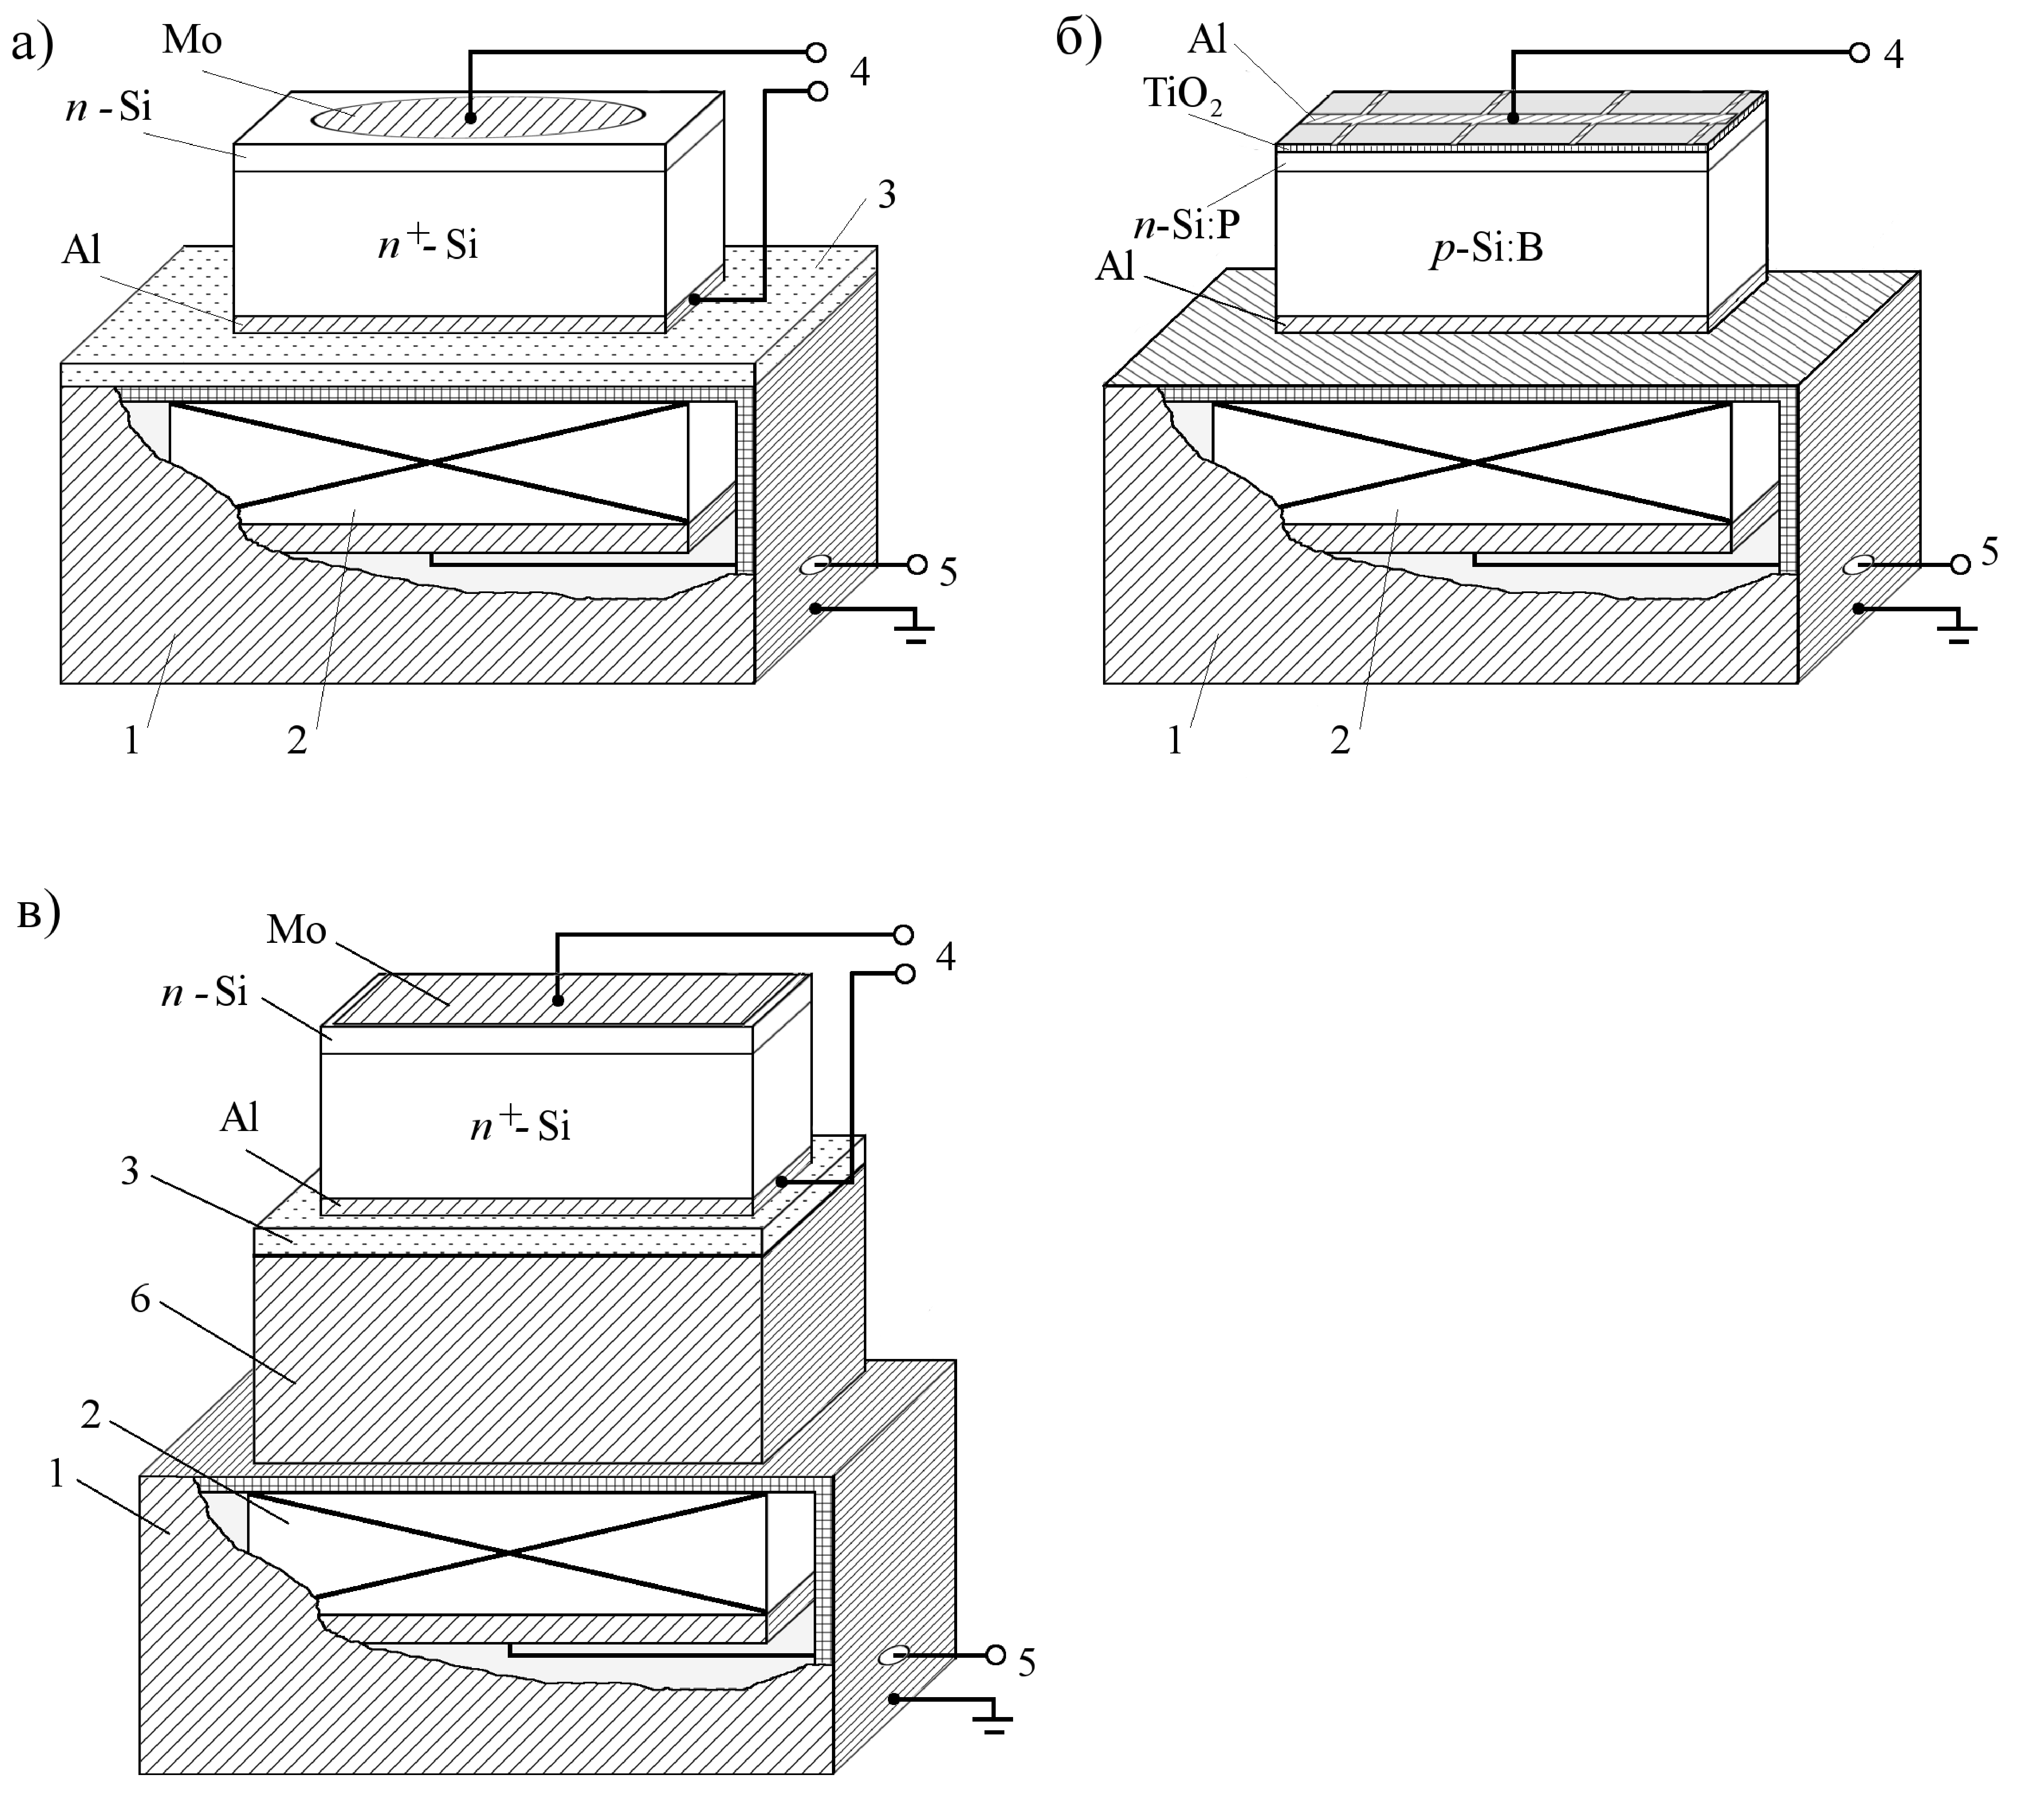
\includegraphics[width=1.0\textwidth]{USL}%
\caption{\label{figUSL}
Використані схеми УЗН кремнієвих структур: \protect\\
1 --  екран (алюмінієва фольга, товщина 0,012~мм);\protect\\
2 -- п'єзоелектричний перетворювач (LiNbO$_3$);\protect\\
3 -- діелектричний прошарок (слюда, товщина 0,03~мм);\protect\\
4 -- контакти для вимірювання вольт--амперних характеристик;\protect\\
5 -- контакти для збудження УЗ;\protect\\
6 -- буфер (алюмінієвий циліндр з високим ступенем паралельності граней, 2~см)
}
\end{figure}



Структури, в яких проводилися дослідження ефектів УЗН, містили енергетичний бар'єр, пов'язаний з наявністю контакту метал--напівпровідник або $p$--$n$ переходу, розміщений поблизу однієї з поверхонь зразка.
Введення УЗ відбувалось з боку грані, протилежної до місця розташування бар'єру.
 Напрям поширення АХ перпендикулярний площині бар'єру і збігається з напрямом струму, який виникає під час прикладення до структури електричної напруги (або при освітленні, якщо об'єктом дослідження є сонячний елемент).
  При використанні повздовжніх хвиль вимушені зміщення атомів відбуваються у тому самому напрямі, тоді як для поперечних хвиль коливання атомів спрямовані у площині бар'єру перпендикулярно до електричного струму .


Раніше показано \cite{Ostapenko1995,YOlikhTPL2011,Ostrovskii2001}, що характерний час зміни властивостей кремнієвих структур під дією УЗ не перевищує 2000~c.
З метою обмеження впливу будь--яких перехідних АІ процесів використовувалася наступна експериментально процедура.
УЗН починалося при кімнатній температурі.
Після цього зразки перебували не менше 60~хв за умов поширення в них пружних коливань і лише після цього, не припиняючи дії УЗ, починалися вимірювання електрофізичних параметрів та/або процеси нагріву або охолодження.


Відомо, що під час навантаження п'єзоелектричний перетворювач нагрівається.
Температура структур, які досліджувалися, контролювалася диференційною термопарою мідь--константан.
В роботі проводилось порівняння значень параметрів, отриманих за однакових температур в умовах УЗН зразків та без нього.
Це дозволяло виокремити АІ зміни характеристик напівпровідникових структур, від змін, пов'язаних з їх розігрівом під час УЗН.
Для оцінки величини впливу УЗ на певний параметр $P$ (напруга холостого ходу, фактор неідеальності, величина зворотного струму тощо),
використовувалися абсолютні
$\Delta P$ чи відносні зміни $\varepsilon_P$
\begin{eqnarray}
  \label{eqAbsDelta} \Delta P &=& P_{in}-P_\mathtt{US}\,, \\
  \label{eqEpsDelta} \varepsilon_P &=& (P_{in}-P_\mathtt{US})/P_{in}\,,
\end{eqnarray}
% \begin{equation}
% \label{eqAbsDelta}
%\Delta P=P_{in}-P_\mathtt{US}\,,
% \end{equation}
%%чи відносні зміни
% \begin{equation}
% \label{eqEpsDelta}
%\varepsilon_P=\frac{P_{in}-P_\mathtt{US}}{P_{in}}\,,
% \end{equation}
де нижні індекси <<$\mathtt{US}$>> та <<$in$>> вказують на те, що відповідне значення параметра було отримане при однаковій температурі за умов УЗН та без нього, відповідно.

При УЗО процеси впливу АХ та вимірювання параметрів були розділені в часу і тому нагальної необхідності екранування п'єзоелектричних полів не було.
Як наслідок, експериментальна схема простіша, п'єзоперетворювач безпосередньо акустично контактував з досліджуваною структурою.


\subsection{Оцінка параметрів акустичного впливу\label{SC:USL}}
%\section{Режими ультразвукового навантаження кристалічних кремнієвих сонячних елементів\label{SC:USL}}


Для оцінки інтенсивності АХ, введеної у напівпровідникову структуру, використовувалася формула плоского п’єзоперетворювача \cite{WusBook}:
 \begin{equation}
 \label{eqWus}
 W_\mathtt{US}=4K_\mathtt{LNO}^2C_\mathtt{LNO}f_r\frac{\rho_\mathtt{LNO}\,\upsilon_\mathtt{LNO}}{\rho_\mathtt{Si}\,\upsilon_\mathtt{Si}}\frac{V_\mathtt{RF}^2}{A_\mathtt{LNO}M_0},
 \end{equation}
де
$K_\mathtt{LNO}$ --- коефіцієнт електромеханічного зв'язку,
$C_\mathtt{LNO}$ та $A_\mathtt{LNO}$ --- статична ємність закріпленого перетворювача та його площа, відповідно;
для використаних перетворювачів ємність складала 0,1$\div$0,3~нФ залежно від площі та товщини;
%$f_r$ --- резонансна частота;
$\rho_\mathtt{LNO}$ та $\rho_\mathtt{Si}$ --- густини LiNbO$_3$ та Si;
$\upsilon_\mathtt{LNO}$ та $\upsilon_\mathtt{Si}$ --- швидкості поширення звуку в LiNbO$_3$ та Si, відповідно;
$V_\mathtt{RF}$ --- амплітуда високочастотної напруги, прикладеної до перетворювача,
а коефіцієнт $M_0$ розраховується за допомогою співвідношення
 \begin{equation}
 \label{eqM0}
 M_0=\frac{\left[\cos\left(\pi\frac{f_\mathtt{US}}{f_r}\right)\right]^2+\left[\frac{\rho_\mathtt{LNO}\,\upsilon_\mathtt{LNO}}{\rho_\mathtt{Si}\,\upsilon_\mathtt{Si}}\sin\left(\pi\frac{f_\mathtt{US}}{f_r}\right)\right]^2}
 {\left[\sin\left(\frac{\pi}{2}\frac{f_\mathtt{US}}{f_r}\right)\right]^4}\,.
 \end{equation}
Відносна деформація при поширенні АХ описується виразом
 \begin{equation}
 \label{eqDefUS}
 \xi_{\mathtt{US}}=\sqrt{\frac{2W_\mathtt{US}}{\rho_\mathtt{Si}\,\upsilon_\mathtt{Si}^3}}\,,
 \end{equation}
тоді як амплітуда зміщень атомів
 \begin{equation}
 \label{eqAmpUS}
 u_{\mathtt{US}}=\sqrt{\frac{W_\mathtt{US}}{2\,\pi^2\,f_\mathtt{US}^2\,\rho_\mathtt{Si}\,\upsilon_\mathtt{Si}}}\,.
 \end{equation}

Параметри, які використовувалися при розрахунках, наведено в табл.~\ref{tabLNO}.


\begin{table}
\caption{\label{tabLNO}Деякі параметри LiNbO$_3$ та Si при кімнатній температурі \cite{WusBook,ShackBook}
}
%\begin{tabular}{|l|l|c|}
%\begin{tabularx}{\textwidth}{|>{\raggedright\arraybackslash}X|>{\centering\arraybackslash}X|>{\centering\arraybackslash}X|}
\begin{tabularx}{\textwidth}{|l|>{\centering\arraybackslash}X|>{\centering\arraybackslash}X|}
\hline
$K_\mathtt{LNO}^2$&зріз $(Y\!+\!36^\circ)$&0,24\\
\cline{2-3}
&зріз $(Y\!+\!163^\circ)$&0,46\\
\hline
$\upsilon_\mathtt{LNO}$,&повздовжні хвилі&7340\\
\cline{2-3}
м/с&поперечні хвилі&4560\\
\hline
&повздовжні хвилі, $[100]$&8430\\
\cline{2-3}
&повздовжні хвилі, $[111]$&9850\\
\cline{2-3}
$\upsilon_\mathtt{Si}$,&повздовжні хвилі, $[110]$&9130\\
\cline{2-3}
м/с&поперечні хвилі, $[110]\,/\,[1\bar{1}0]$&4670\\
\cline{2-3}
&поперечні хвилі, $[110]\,/\,[001]$&5840\\
\cline{2-3}
&поперечні хвилі, $[111]\,/\,$довіл.&5090\\
\hline
\multicolumn{2}{|l|}{$\rho_\mathtt{LNO}$, кг/м$^3$}&4700\\
\hline
\multicolumn{2}{|l|}{$\rho_\mathtt{Si}$, кг/м$^3$}&2328\\
\hline
%\end{tabular}
\end{tabularx}
\end{table}

Дослідження, результати яких наведено в розділах~\ref{Ch_SSC}, \ref{Ch_GammaSD} та \ref{Ch_UST_MW},  проводились у достатньо вузькому температурному діапазоні $290\div340$~К.
При цьому вважалось, що параметри п'зоелектричного перетворювача змінюються мало, сталість величини $V_\mathtt{RF}$ забезпечує незмінність $W_\mathtt{US}$  для всього діапазону температур.
Вплив екрануючого прошарку на інтенсивність звуку, введеного в зразок, вважався знехтувано малим, оскільки його товщина значно менша ніж половина довжини АХ.

\subsection{Особливості низькотемпературного ультразвукового \mbox{навантаження}\label{SSDB:USL}}

Ультразвукове навантаження структур Mo---$n$--$n^+$--Si (розділ~\ref{Ch_USL_T_SD}) здійснювалося в діапазоні температур 130$\div$330~К за схемою, наведеною на рис.~\ref{figUSL},в.
У випадку низькотемпературного (при $T<230$~К) УЗН процес збудження АХ був утруднений через те, що
рідкі акустичні склейки на кшталт вакуумного масла кристалізувалися і переставали виконувати свою функцію.
В той же час, контакт створений при кімнатній температурі за допомогою жорсткої склейки (піцеїн або БФ6),
руйнувався при охолодженні внаслідок різниці коефіцієнтів теплового розширення.
В роботі низькотемпературне УЗН (повздовжні хвилі) здійснювалося за допомогою свіжого (до 5~год після нанесення) контакту з клею БФ6,
який ще не повністю кристалізувався.
Наявність акустичного контакту контролювалася за виглядом залежності повного опору перетворювача від частоти,
де за наявності акустичного контакту з'являвся ряд максимумів, пов'язаних з відбиванням хвиль від граней буфера.

\begin{figure}
\center
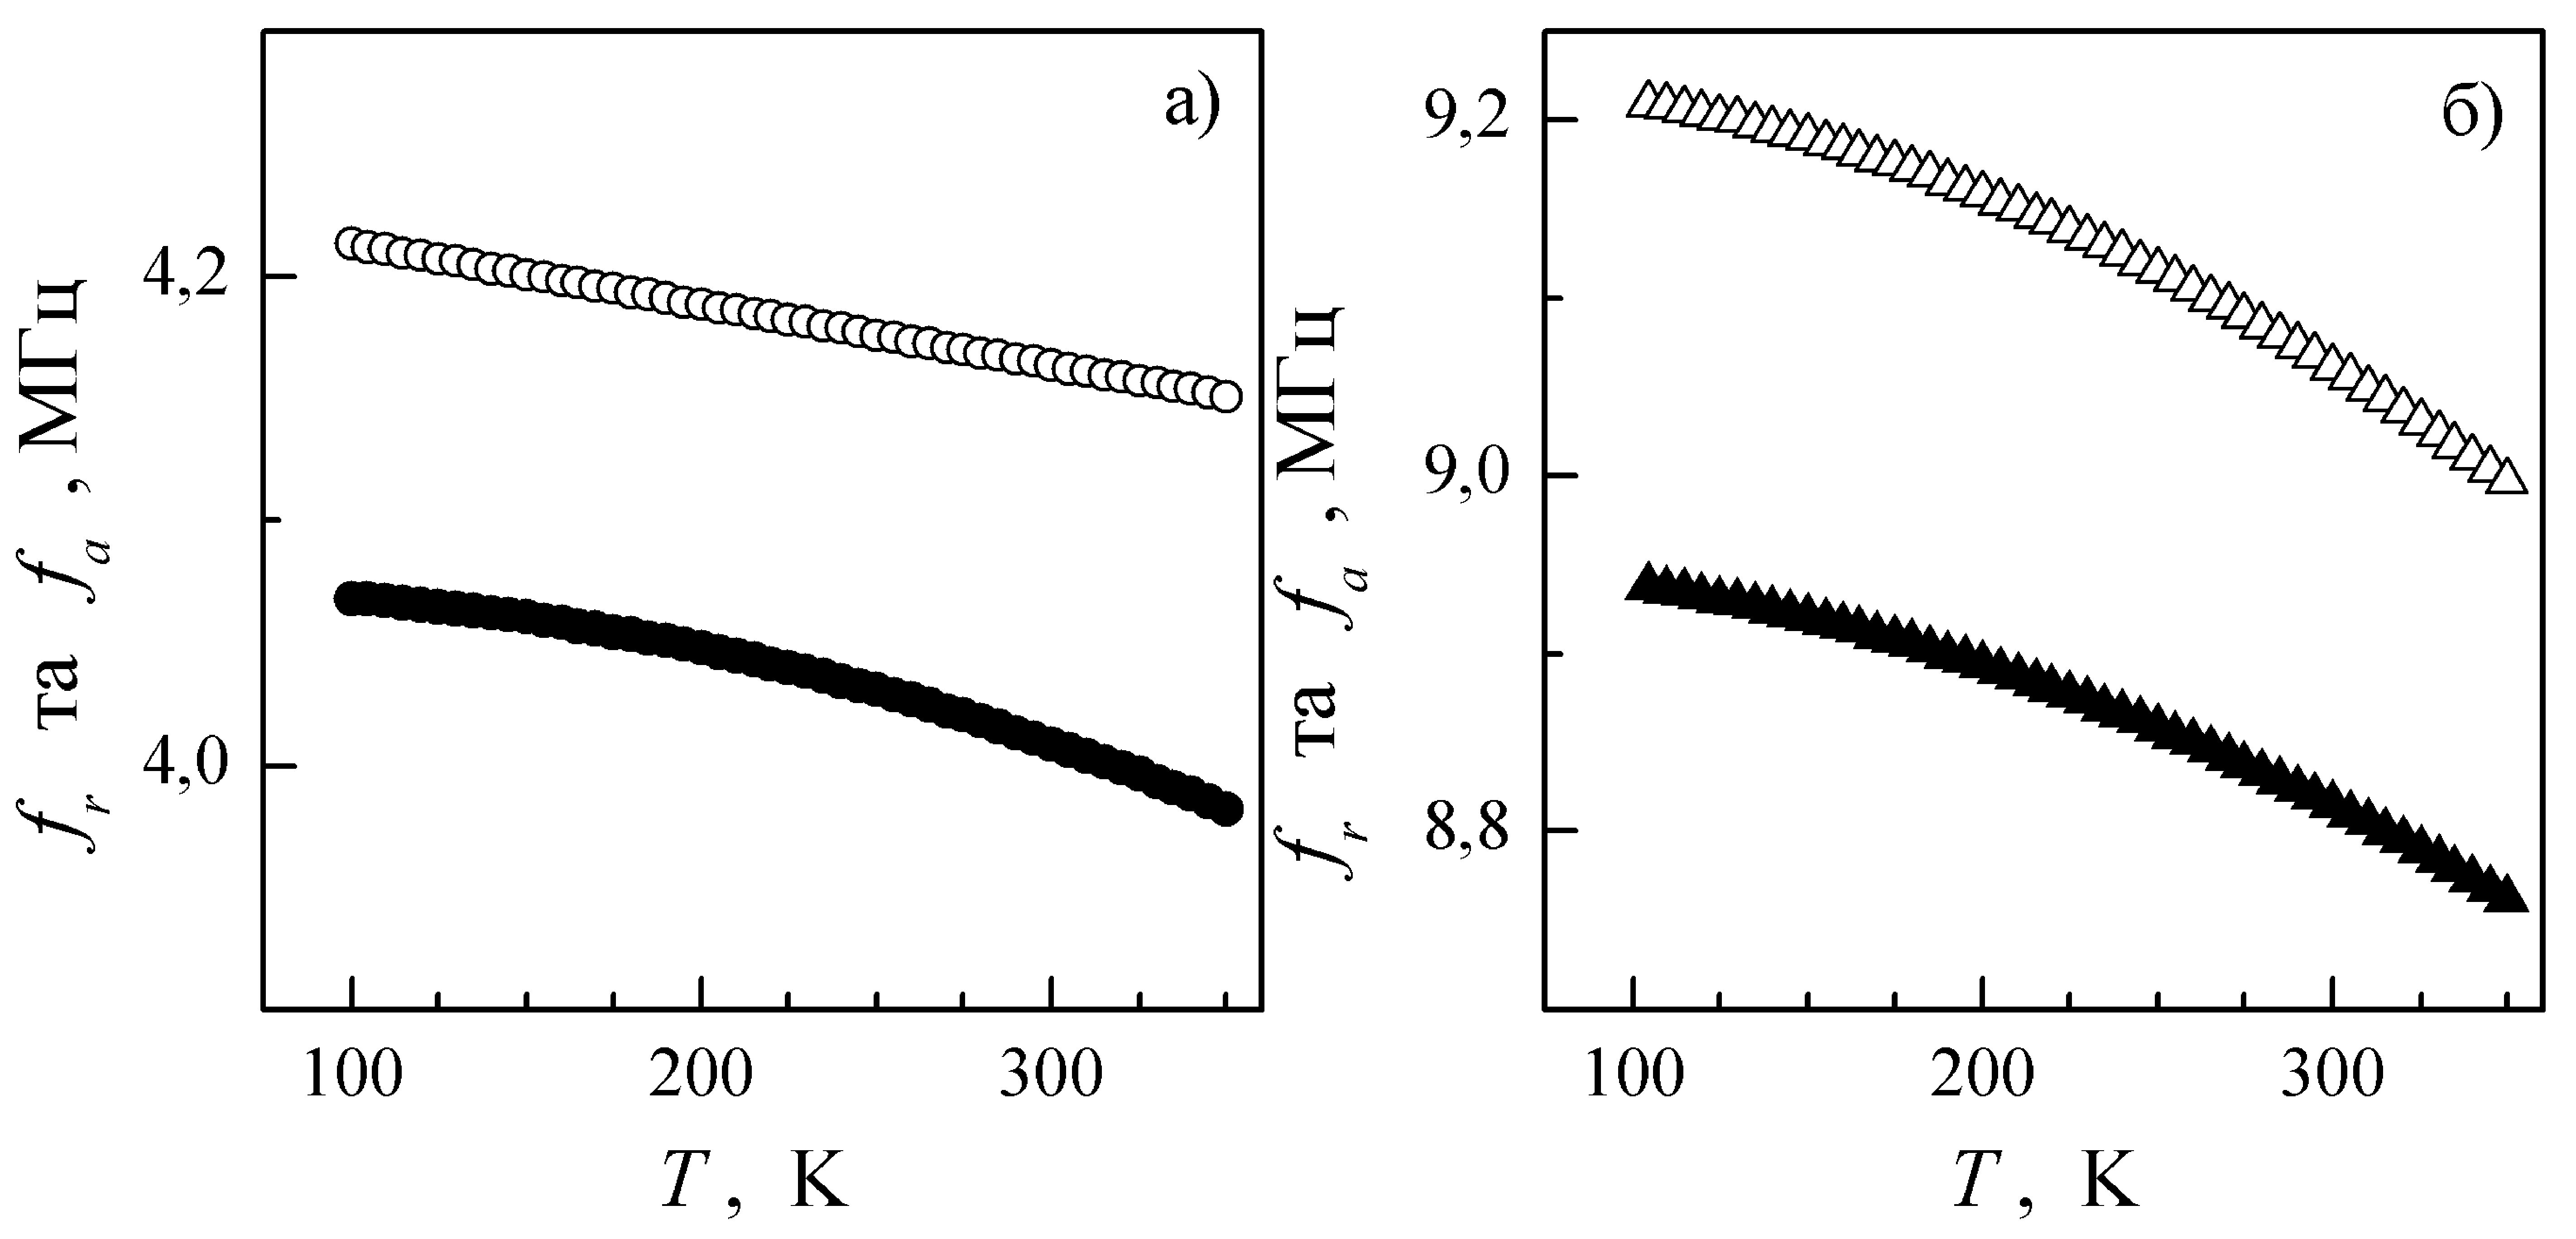
\includegraphics[width=0.8\textwidth]{figFrT}%
\caption{\label{figFrT}
Температурна залежність частот резонансу (заповнені точки) та антирезонансу (порожні точки) (перша гармоніка)
п'єзоелектричних перетворювачів LiNbO$_3$ з робочими частотами $f_\mathtt{US}$ 4,1~МГц (а) та 9,6 (б)~МГц при кімнатній температурі
}
\end{figure}


Водночас при визначенні параметрів УЗН за допомогою формул (\labelcref{eqAmpUS,eqWus,eqM0,eqDefUS}) та даних табл.~\ref{tabLNO} викликає ряд труднощів.
По--перше, параметри матеріалу є температурозалежними.
Наприклад, з літератури відомо, що зміна пружних сталих при збільшенні температури на 100 К для LiNbO$_3$ становить приблизно (-2\%) \cite{LNO_C:Temp},
а для кремнію --- (-2.5\%) \cite{Si_C:Temp};
типові температурні залежності резонансної та антирезонансної частот показані на рис.~\ref{figFrT}.
Широкий температурний інтервал дослідження АІ ефектів не дозволяв нехтувати подібними залежностями.
%При дослідженні АІ ефектів в структурах SSDB вимірювання проводилися в достатньо широкому температурному інтервалі і тому подібними залежностями нехтувати не можна.
По--друге, наявність буфера була причиною втрат акустичної енергії внаслідок поглинання УЗ в алюмінієвому циліндрі, часткового відбивання пружних хвиль
при переході з одного середовища в інше тощо.
Ці ефекти також не враховані у виразах (\ref{eqWus}) і  (\ref{eqM0}).
Враховуючи зазначене вище, оцінка інтенсивності введеного УЗ здійснювалася за допомогою виразу
 \begin{equation}
 \label{eqWus2}
 W_\mathtt{US}=\frac{V_\mathtt{RF}^2}{2\,A_\mathtt{LNO}\,Z_\mathtt{LNO}}\,K_\mathtt{LNO}^2\,l_\mathtt{US},
 \end{equation}
де
$Z_\mathtt{LNO}$ --- імпеданс акустично навантаженого перетворювача,
$l_\mathtt{US}$ --- коефіцієнт, який враховує загальні втрати пружної енергії.
При цьому вважалося, що величини
$K_\mathtt{LNO}$, $Z_\mathtt{LNO}$ та $l_\mathtt{US}$ залежать від температури.

Визначення $K_\mathtt{LNO}$ та $l_\mathtt{US}$ відбувалося з використанням стандартної схеми,
зображеної на рис.~\ref{Luna2},а.
У системі збуджувалися імпульси УЗ за допомогою одного з ідентичних п'єзоперетворювачів і реєструвалися
високочастотні сигнали на другому.
Амплітуди сигналів $V_\mathtt{RF}^{(1)}$ та $V_\mathtt{RF}^{(2)}$, пов'язаних з однократним та троєкратний (після відбиття від правої та лівої границь) проходженням акустичного імпульсу через систему
(рис.~\ref{Luna2},б) можуть бути записані у вигляді
\begin{eqnarray}
  \label{eqVrf1} (V_\mathtt{RF}^{(1)})^2&=&V_\mathtt{RF}^2\,K_\mathtt{LNO}^4\,l_\mathtt{US}, \\
  \label{eqVrf2} (V_\mathtt{RF}^{(2)})^2&=&V_\mathtt{RF}^2\,K_\mathtt{LNO}^4\,l_\mathtt{US}^3.
\end{eqnarray}

% \begin{equation}
% \label{eqVrf1}
% (V_\mathtt{RF}^{(1)})^2=V_\mathtt{RF}^2\,K_\mathtt{LNO}^4\,l_\mathtt{US},
% \end{equation}
% \begin{equation}
% \label{eqVrf2}
% (V_\mathtt{RF}^{(2)})^2=V_\mathtt{RF}^2\,K_\mathtt{LNO}^4\,l_\mathtt{US}^3.
% \end{equation}

\begin{figure}
\center
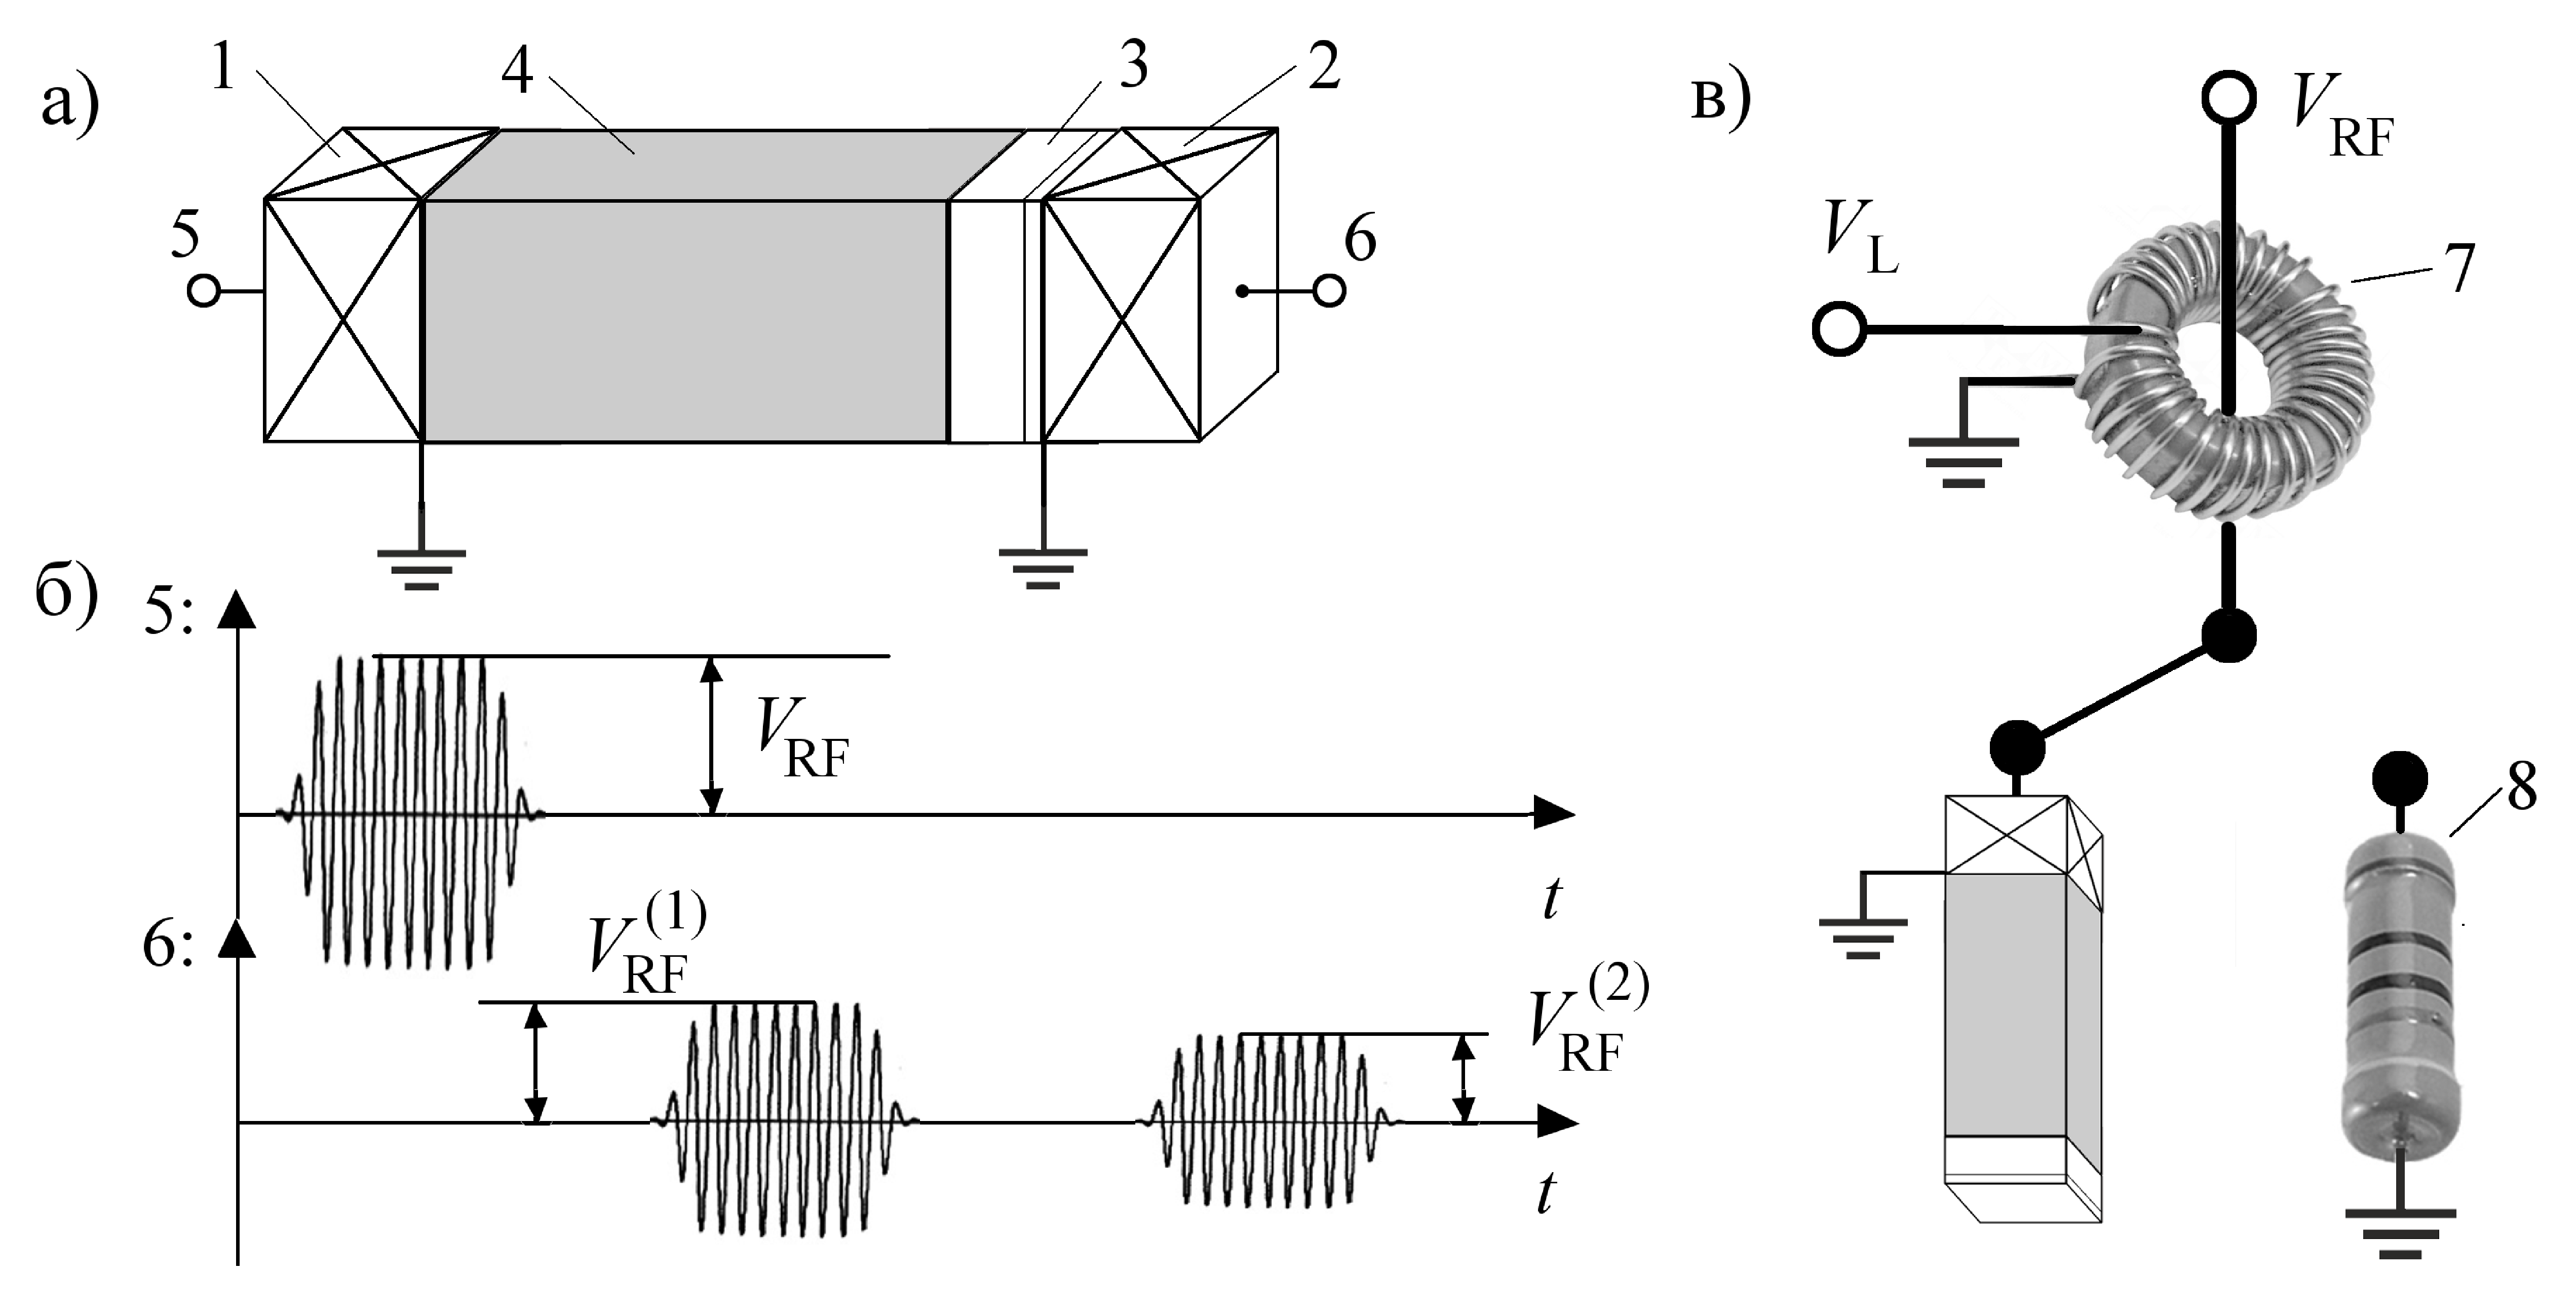
\includegraphics[width=0.9\textwidth]{Luna2}%
\caption{\label{Luna2}
а) Схема для оцінки інтенсивності введеного УЗ:\protect\\
1, 2 -- ідентичні п'єзоелектричні перетворювачі; \protect\\
3 -- напівпровідникова структура;\protect\\
4 -- буфер; \protect\\
5, 6 --- електроди збуджуючого та приймаючого перетворювачів, відповідно. \protect\\
б) Схематична осцилограма сигналів на електродах п'єзоперетворювачів. \protect\\
в) Схема для визначення імпедансу п'єзоперетворювача: \protect\\
7 -- датчик струму; \protect\\
8 -- еталонний опір
}
\end{figure}

Останні два співвідношення дозволяють визначити акустичні параметри системи на основі вимірювання амплітуд
високочастотних сигналів на електродах збуджуючого та приймаючого п'єзоперетворювачів.
Приклад отриманих температурних залежностей наведено на рис.~\ref{figKp2T}.

\begin{figure}
\center
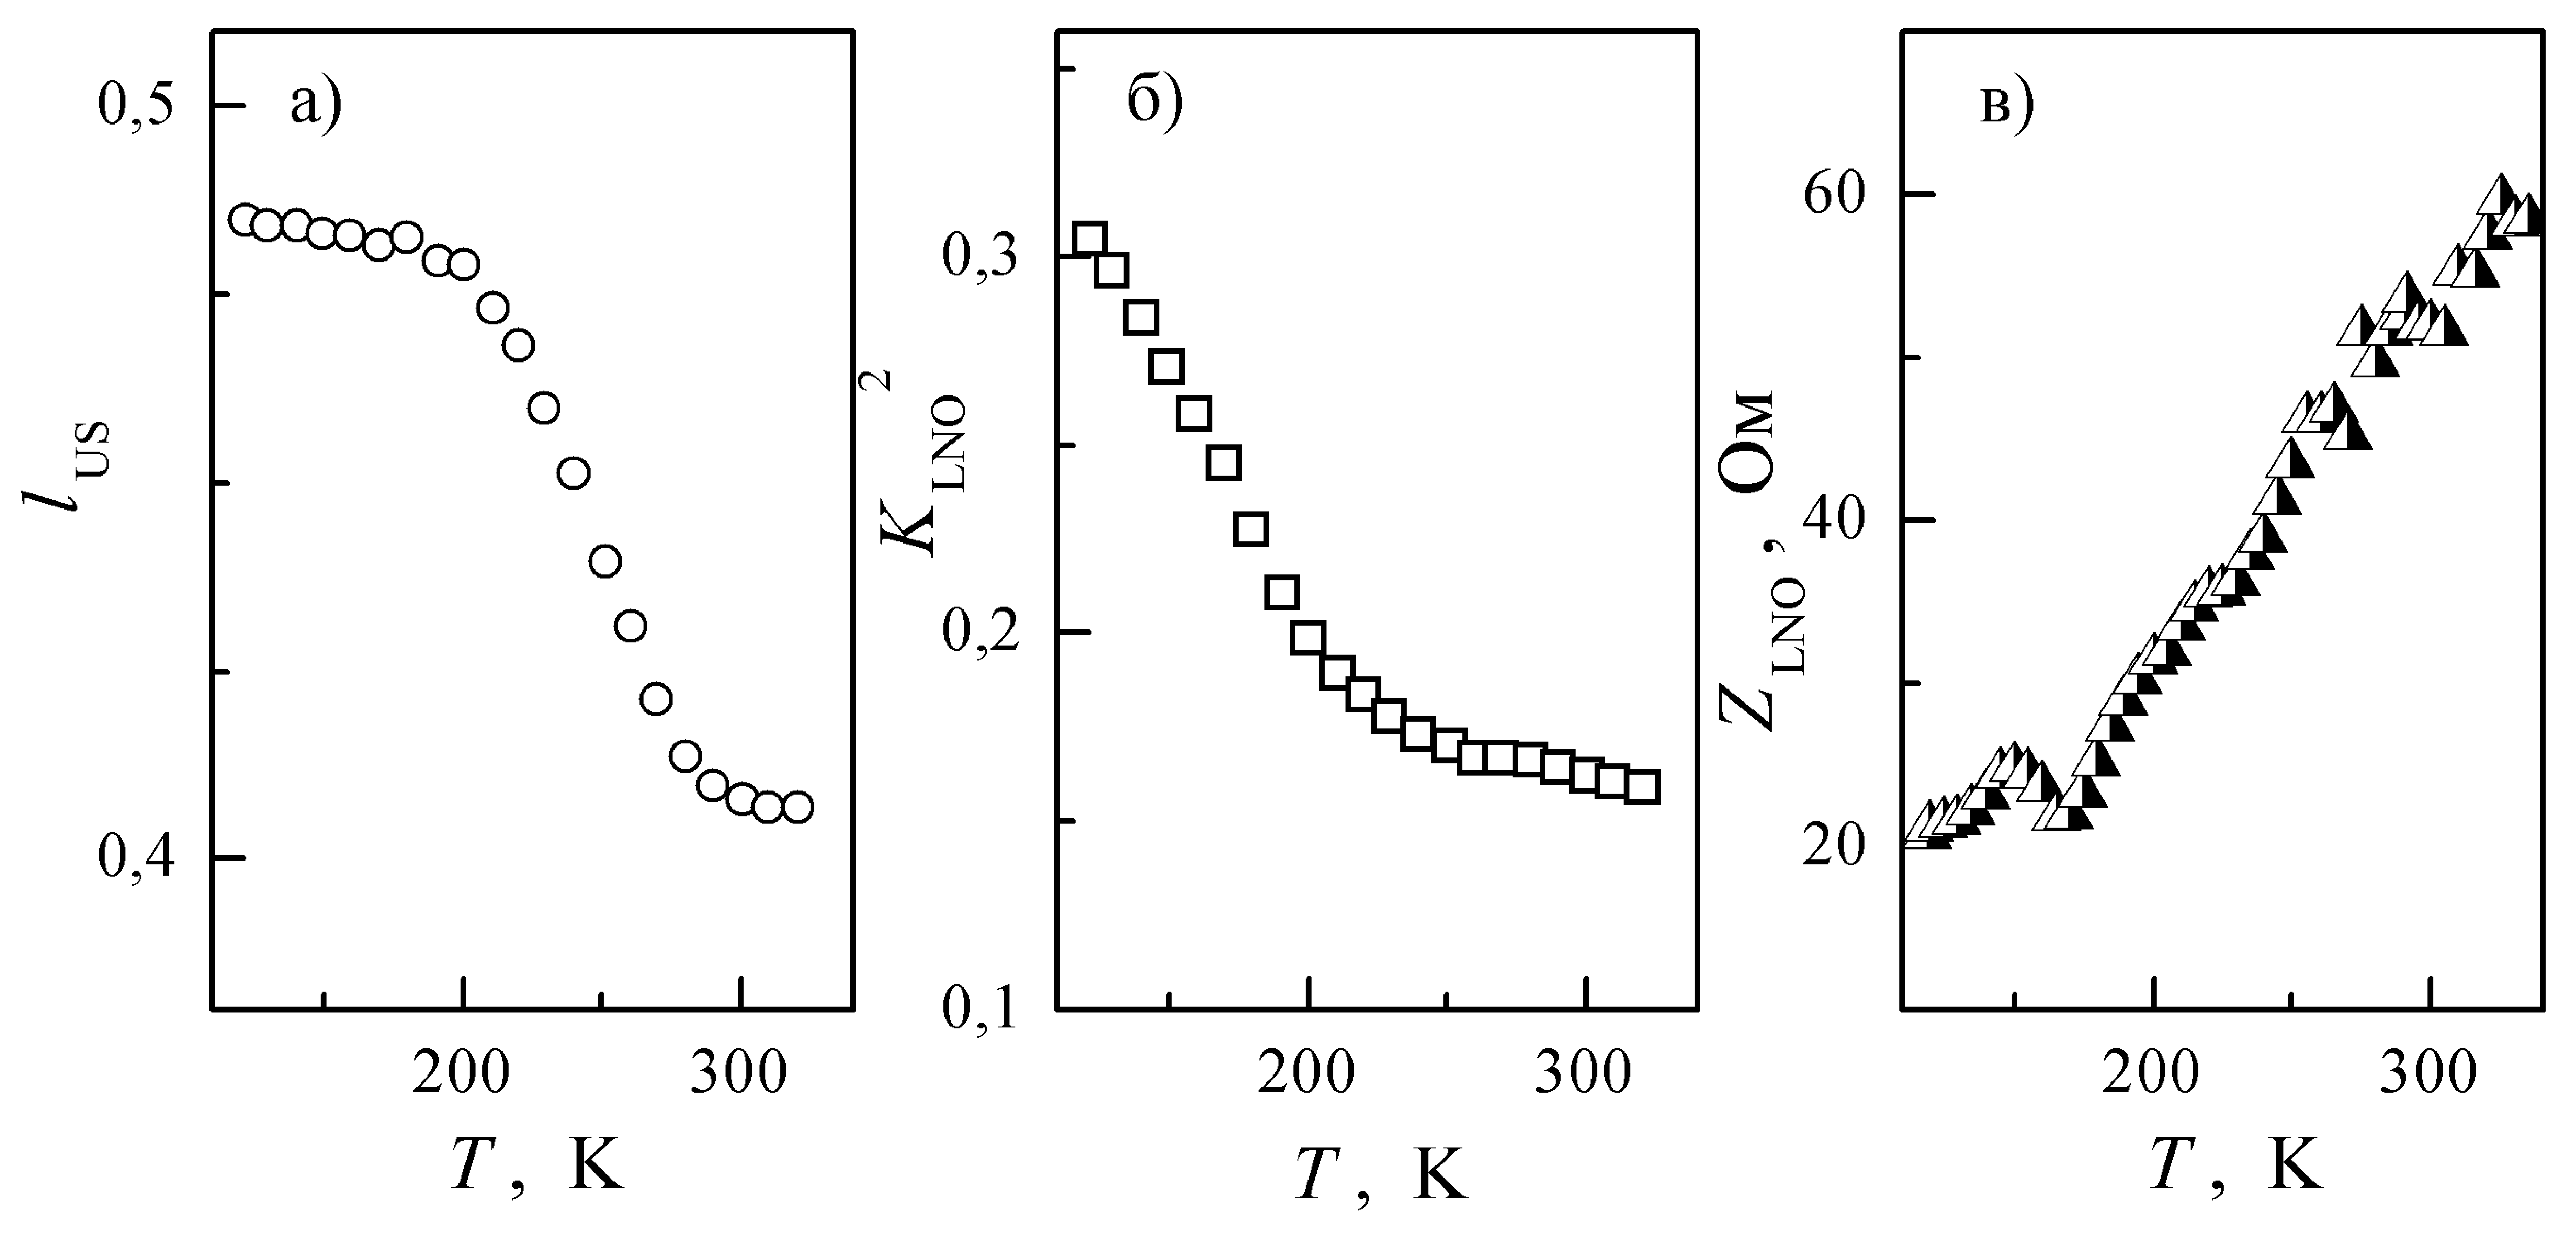
\includegraphics[width=0.9\textwidth]{figKp2T}%
\caption{\label{figKp2T}
Температурні залежності коефіцієнта акустичних втрат (а),
квадрата коефіцієнта електромеханічного зв'язку (б) та
імпедансу (в) п'єзоперетворювача з робочою частотою $f_\mathtt{US}=8,4$~МГц}
\end{figure}

Для оцінки $Z_\mathtt{LNO}$ використовувався метод,
схема якого представлена на рис.~\ref{Luna2},в.
Датчиком струму слугувало феритове кільце із дротяною обмоткою.
Кількість витків обмотки підбиралось для кожної частоти таким чином, щоб для випадку, коли під'єднано еталонний опір $R_\mathtt{st}$,
зсув фаз між збуджуючим сигналом амплітудою $V_\mathtt{RF,st}$ та сигналом з датчика амплітудою $V_\mathtt{L,st}$
дорівнював нулеві.
Величина імпедансу розраховувалася за допомогою виразу
 \begin{equation}
 \label{eqZlno}
 Z_\mathtt{LNO}=\frac{V_\mathtt{RF}}{V_\mathtt{L}}\,\frac{V_\mathtt{L,st}}{V_\mathtt{RF,st}}\,R_\mathtt{st}.
 \end{equation}

В роботі використовувався еталонний опір величиною 56,7~Ом.
Температурна залежність імпедансу одного з перетворювачів наведена на рис.~\ref{figKp2T},в.

Використання виразу (\ref{eqWus2}) та даних рис.~\ref{figKp2T} показує, що при подачі на електроди п'єзоелектричного перетворювача
високочастотної напруги з постійною амплітудою в діапазоні температур 130$\div$330~K призводить до поширення у зразку АХ з
інтенсивністю, яка змінюється більше ніж в п'ять разів --- рис.~\ref{figWusT},а.
З іншого боку, поблизу кімнатних температур наближення попереднього пункту, про те, що сталому значенню
$V_\mathtt{RF}$ відповідає постійна величина $ W_\mathtt{US}$, справедливе з точністю до 10 відсотків.
На рис.~\ref{figWusT},б також показано як має змінюватись амплітуда напруги на п'єзоперетворювачі, щоб при різних температурах
інтенсивність УЗН залишалась постійною.


\begin{figure}
\center
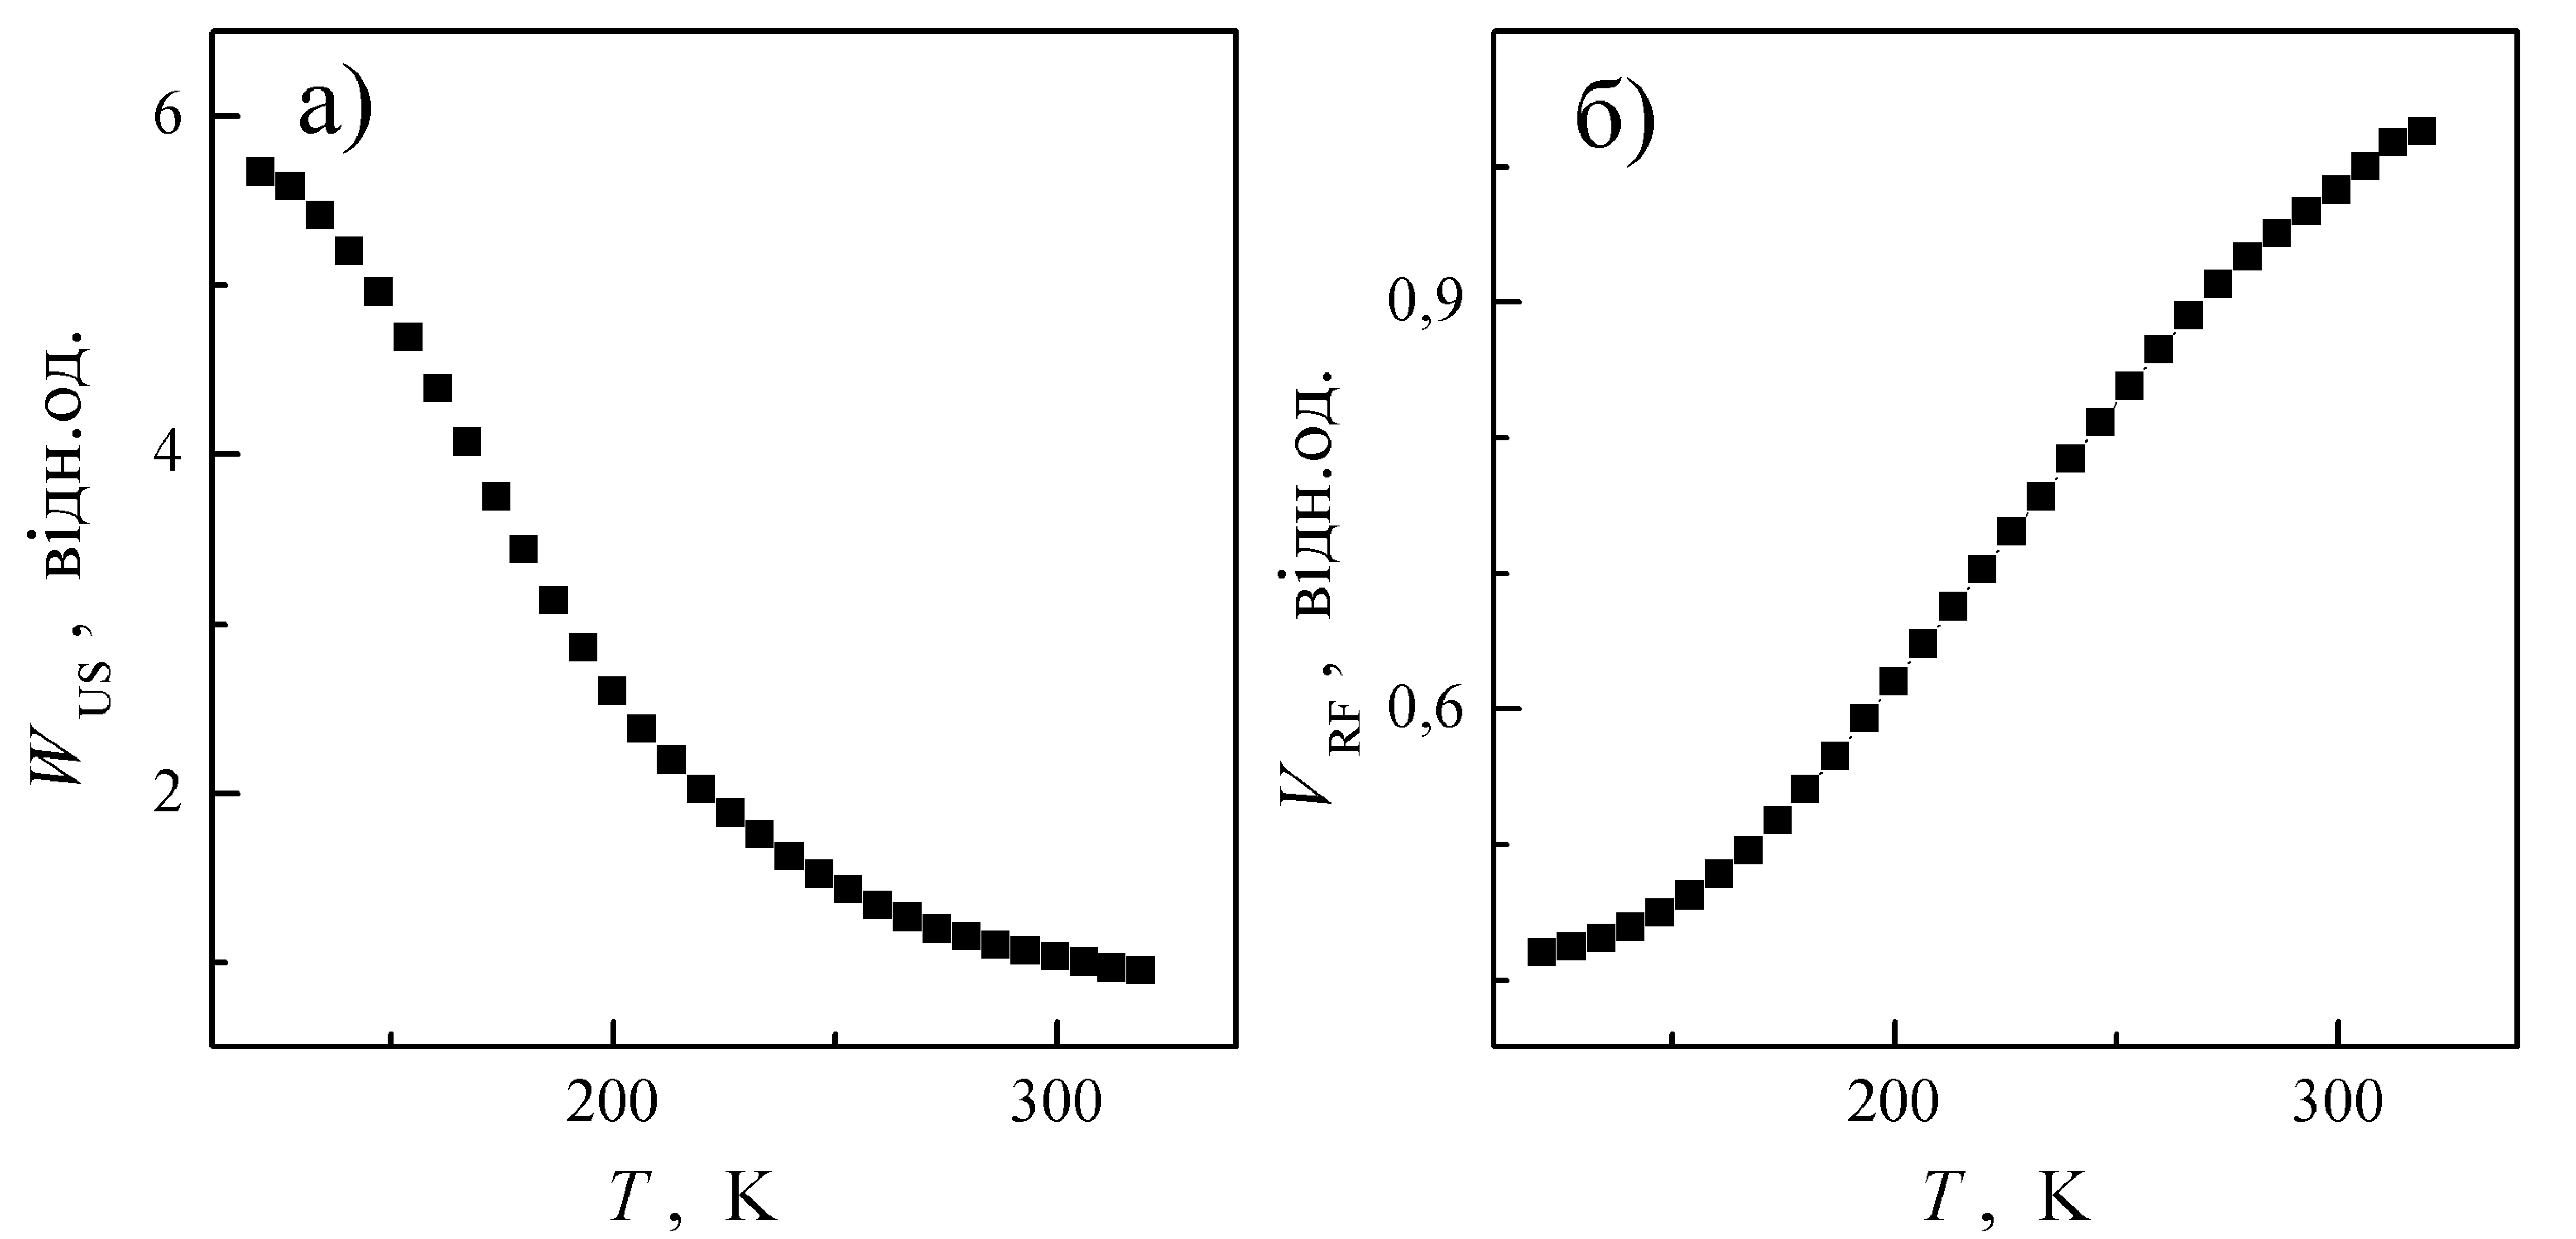
\includegraphics[width=0.8\textwidth]{figWusT}%
\caption{\label{figWusT}
Температурні залежності
інтенсивності введеного УЗ при постійному значенні амплітуди напруги на п'єзоперетворювачі (а)
та необхідної амплітуди на п'єзоперетворювачі для постійності інтенсивності введеного УЗ (б)
для п'єзоперетворювача з робочою частотою $f_\mathtt{US}=8,4$~МГц.
}
\end{figure}







\chapter{Особливості використання активного ультразвуку}
Значна частина представлених у дисертаційній роботі результатів пов'язана з дослідженням ефектів, які відбуваються в напівпровідникових структурах внаслідок
поширення в них акустичних хвиль (АХ) мегагерцевого діапазону.
У зв'язку з тим, що використання ультразвуку (УЗ), на жаль, ще не є стандартним способом впливу на напівпровідникові кристали,
у цьому розділі представлено узагальнена  інформація щодо відповідних експериментальних методик.

Зокрема, представлені описи процедур ультразвукової обробки (УЗО) та ультразвукового навантаження (УЗН).
Відмінності у використанні цих термінів пов'язані з оборотністю АІ процесів.
Так, в першому випадку (УЗО), внаслідок поширення пружних хвиль відбуваються незворотні (залишкові) зміни властивостей напівпровідникових структур.
Тоді як в другому випадку (УЗН), ефекти є оборотніми (динамічними), зміни електрофізичних параметрів спостерігаються лише за умов поширення АХ;
після припинення дії УЗ параметри поступово повертаються до своїх вихідних (до початку УЗН) значень.



\section{Методика вивчення ультразвукового впливу}
%В роботі наведено результати досліджень акустоіндукованих (АІ) ефектів в кремнієвих бар'єрних структурах, описаних в розділах \ref{MSSi} та \ref{SSC}.
%Це ефекти полягають у зміні електрофізичних параметрів структур під час поширення в них пружних коливань, тобто під час ультразвукового навантаження (УЗН).
%Ефекти є оборотніми (динамічними), після припинення поширення акустичних хвиль (АХ) параметри поступово повертаються до своїх вихідних (до початку УЗН) значень.
%
Для збудження УЗ у досліджуваних структурах використовувалися п'єзоелектричні перетворювачі,
виготовлені з пластин ніобату літію (LiNbO$_3$) з металізацією обох граней шляхом вакуумного напилення алюмінію.
Для збудження повздовжніх та поперечних акустичних хвиль використовувалися пластини зі зрізом $(Y\!+\!36^\circ)$ та , відповідно.

З літератури \cite{Ostapenko1995,Davletova2008,Davletova2009,Pashaev2014r} відомо, що АХ з частотою, що знаходиться в діапазоні $1\div30$~МГц, здатні впливати на стан дефектів у кремнії.
Саме такий частотний діапазон був використаний у представлених дослідженнях.
В експериментах проводилось збудження УЗ з частотою $f_\mathtt{US}$, яка знаходилась поблизу першої або третьої гармоніки товщинного резонансу пластинки.
Безпосереднє значення $f_\mathtt{US}$, при якому введення пружних коливань у зразок відбувається найбільш ефективно, визначалось стандартним методом за максимальною амплітудою коливань краплі води (або вакуумного масла), розміщеної на поверхні перетворювача, при прикладанні до його граней змінної напруги.

Попередні дослідження різних авторів \cite{Davletova2008,Davletova2009,Pashaev2014r,Vlasov2009r} показали, що використання УЗ з інтенсивністю $W_\mathtt{US}\geq1$~Вт/см$^2$ спричинює необоротні (залишкові) зміни властивостей кремнієвих структур, які пов'язані з відпалом радіаційних дефектів, формуванням нових дефектів або переміщенням вже існуючих, на відстані, що значно перевищують міжатомну відстань.
Так як метою частини роботи було дослідження саме оборотних АІ ефектів, то УЗН проводилось при $W_\mathtt{US} \leq 0,5$~Вт/см$^2$.
Детальніше процедура оцінки $W_\mathtt{US}$ та інших параметрів УЗ впливу наведена у розділі \ref{subLowT}.

Для того, щоб під час УЗН позбавитися впливу п'єзоелектричного поля, яке супроводжує механічні коливання пластини LiNbO$_3$,  як на параметри напівпровідникових структур, так і на процес вимірювання електрофізичних параметрів,
перетворювач екранувався.
Як наслідок, можна стверджувати, що виявлені під час УЗН ефекти визначаються лише знакозмінною деформацією.

Схеми навантаження зразка, які використовувалися в роботі, наведено на Рис.~\ref{figUSL}.
Наявність чи відсутність діелектричного прошарку визначалась особливостями вимірювання ВАХ.
Використання буфера дозволяло найефективніше мінімізувати вплив п'єзоперетворювача на процеси у напівпровіднику:
металевий буфер виконував роль як електричного, так і температурного екрану.
Тип схеми УЗН, яка використовувалася в тих чи інших дослідах, зазначено на початку відповідного розділу.

\begin{figure}
\center
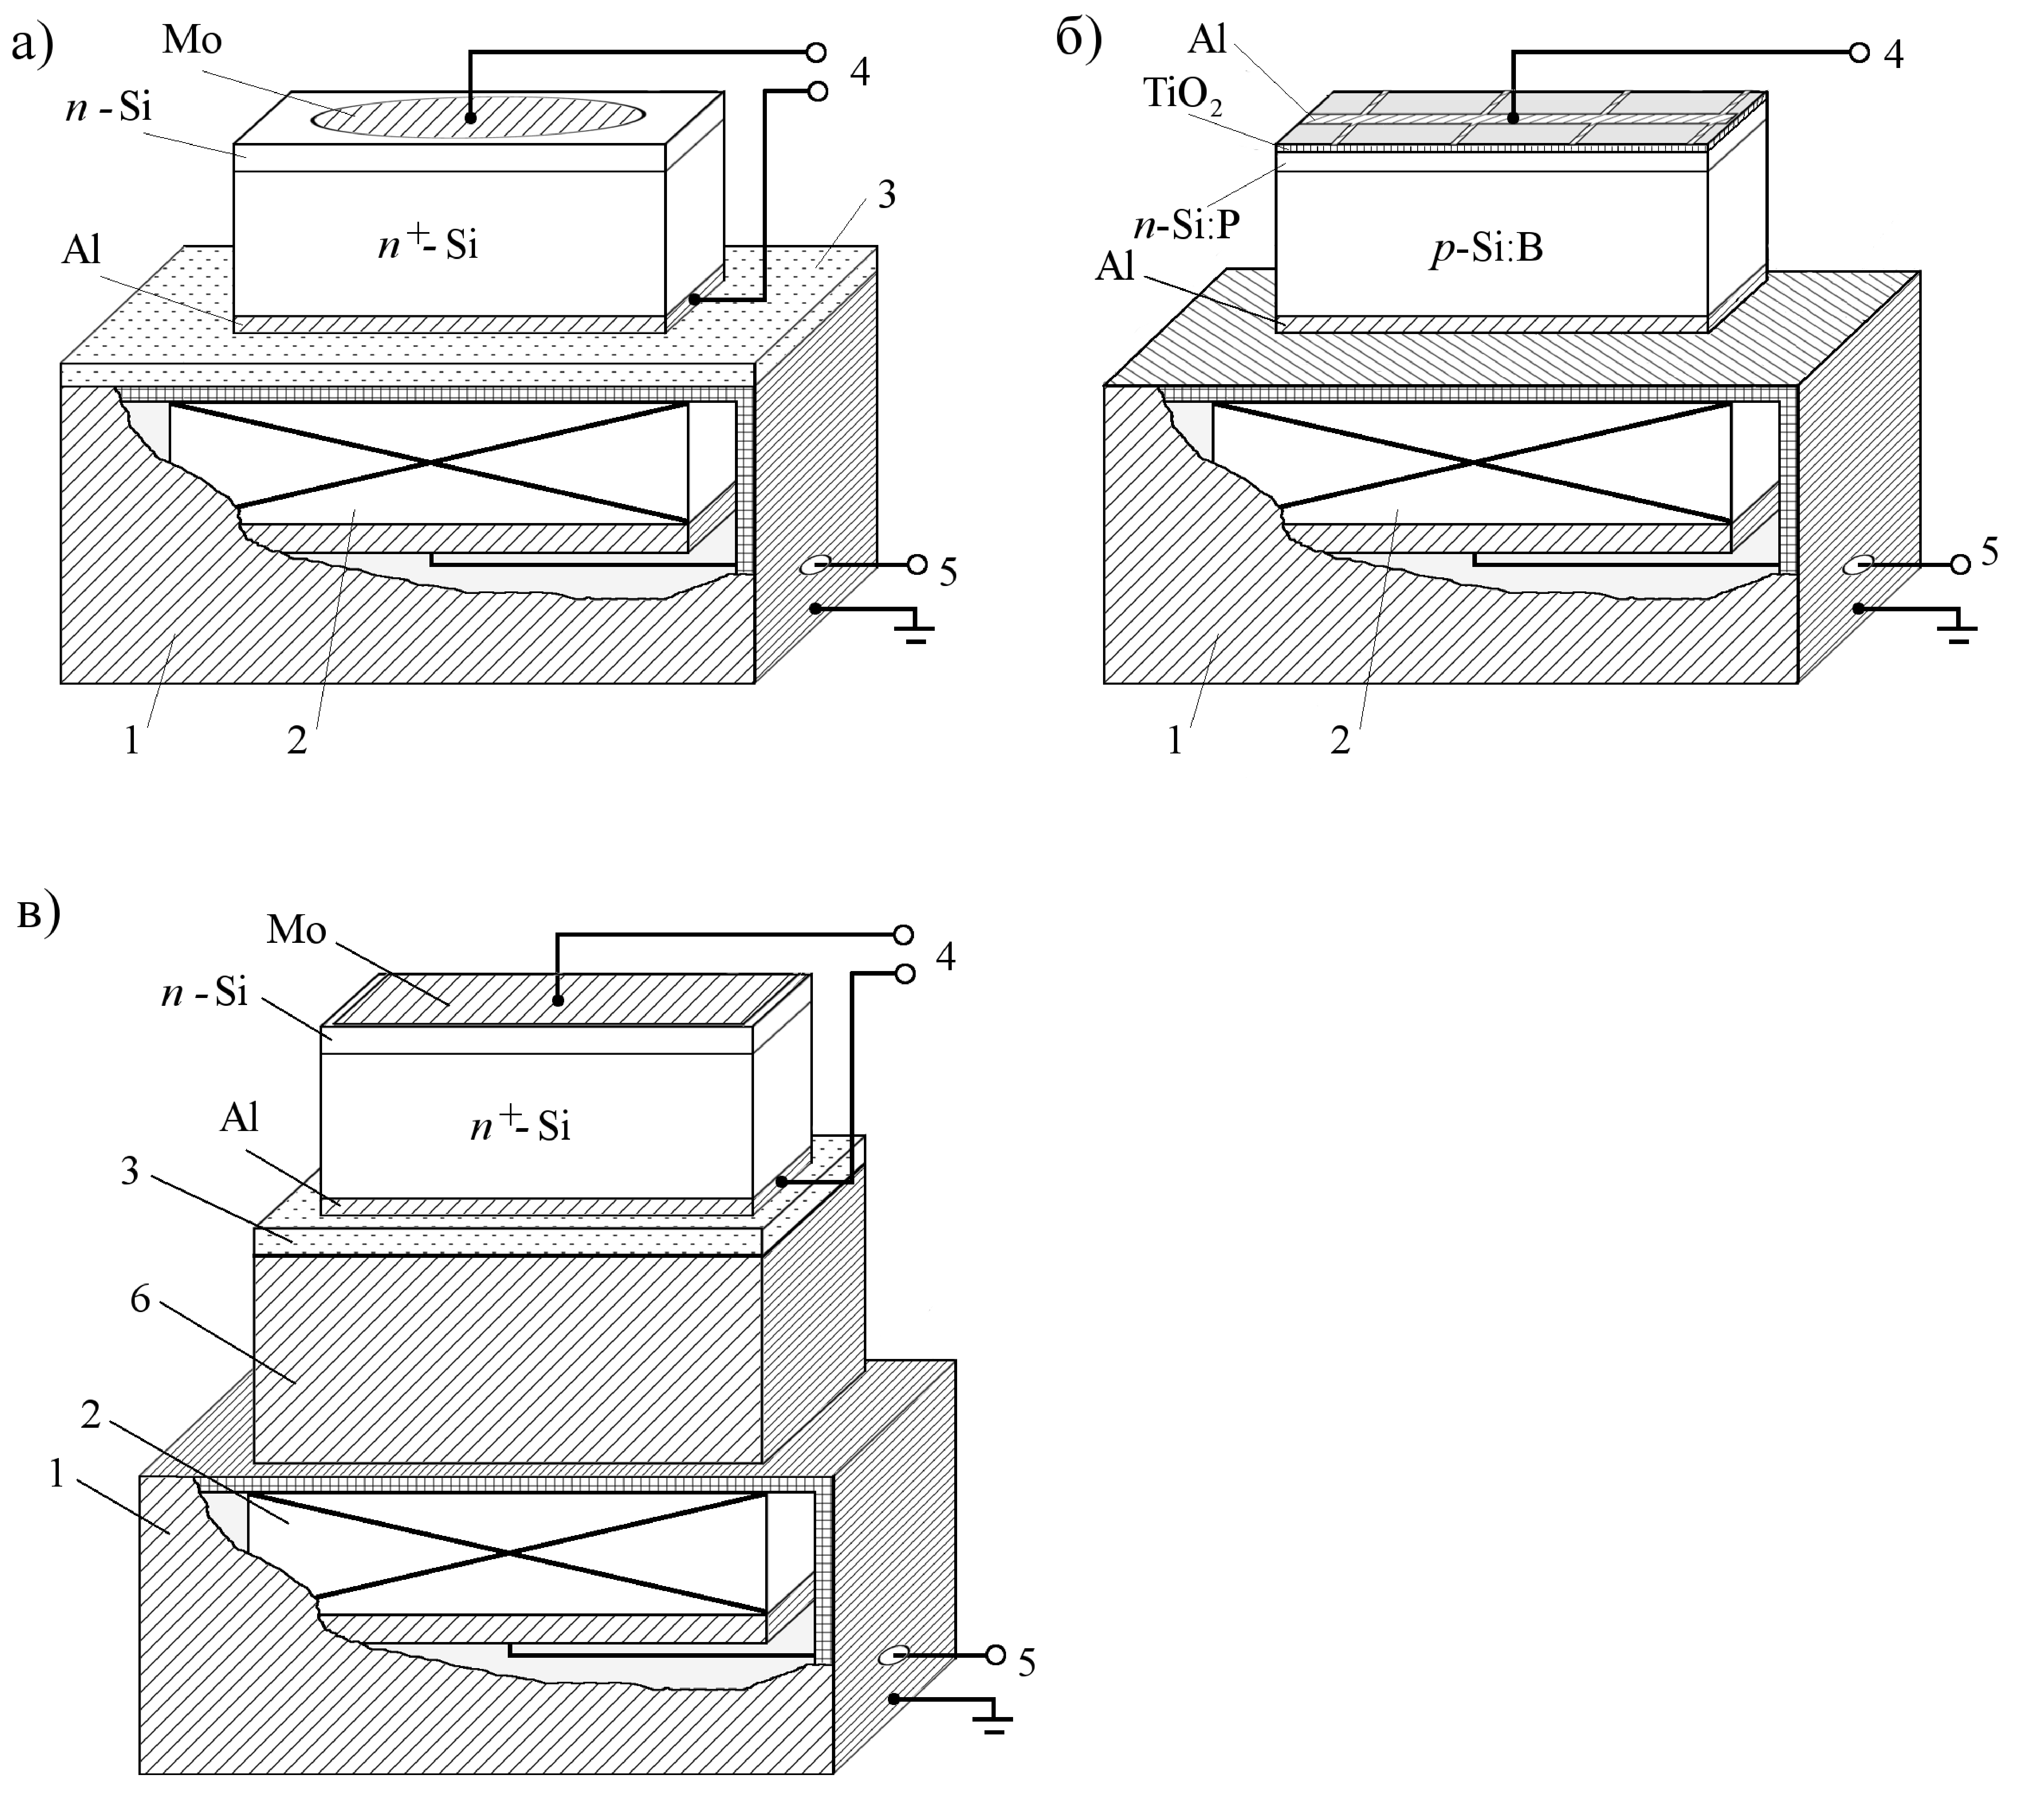
\includegraphics[width=1.0\textwidth]{USL}%
\caption{\label{figUSL}
Використані схеми УЗН.
1 --  екран (алюмінієва фольга);
2 --- п'єзоелектричний перетворювач (LiNbO$_3$);
3 --- діелектричний прошарок (слюда);
4 --- контакти для вимірювання ВАХ;
5 --- контакти для збудження УЗ;
6 --- буфер (циліндр Al з високим ступенем паралельності граней, довжина 2~см)
}
\end{figure}

Структури, в яких проводилися дослідження ефектів УЗН, містили енергетичний бар'єр, пов'язаний з наявністю контакту МН або p--n переходу і розміщений поблизу однієї з поверхонь зразка.
Введень УЗ відбувалось з боку грані, протилежної до місця розташування бар'єру.
Тобто, напрям поширення АХ перпендикулярний площині бар'єру і співпадає з напрямом струму, який виникає під час прикладення до структури електричної напруги (або при освітленні, якщо об'єктом дослідження є сонячний елемент).
При цьому, при використанні повздовжніх хвиль вимушені зміщення атомів відбуваються у тому самому напрямі, тоді як для поперечних хвиль коливання частинок спрямовані перпендикулярно до електричного струму у площині бар'єру.


Для створення акустичного контакту при різних УЗН використовувалися вакуумне масло, клей БФ6, піцеїн.
Зауважимо, що у випадку низькотемпературного (при $T<230$~К) УЗН процес збудження АХ був утруднений через те, що
рідкі акустичні склейки на кшталт вакуумного масла кристалізувалися і переставали виконувати свою функцію.
В той же час, контакт створений при кімнатній температурі за допомогою жорсткої склейки (піцеїн або БФ6),
руйнувався при охолодженні внаслідок різниці коефіцієнтів теплового розширення.
В роботі проведення низькотемпературних УЗН при використанні повздовжніх хвиль здійснювалось за допомогою свіжого (до 5~год після нанесення) контакту з клею БФ6, який ще не висох.
Наявність акустичного контакту контролювалася за виглядом залежності повного опору перетворювача від частоти (АЧХ, амплітудно--частотної характеристики).
Зокрема, при використанні схеми, зображеної на Рис.~\ref{figUSL},в, за наявності акустичного контакту на АЧХ з'являвся ряд максимумів, пов'язаних з відбиванням хвиль від граней буфера.


Раніше показано \cite{Ostapenko1995,YOlikhTPL2011,Ostrovskii2001}, що характерний час зміни властивостей кремнієвих структур під дією УЗ не перевищує $2\cdot10^3$~c.
Для того, щоб дочекатися закінчення всіх перехідних АІ процесів, використовувалася наступна експериментально процедура.
УЗН починалась при кімнатній температурі.
Після цього зразки перебували не менше 60~хв за умов поширення в них пружних коливань і лише після цього, не припиняючи дії УЗ, починалось вимірювання електрофізичних параметрів та/або процеси нагріву або охолодження.

Відомо, що під час навантаження п'єзоперетворювач нагрівається.
Температура кремнієвих структур контролювалася диференційною термопарою мідь--константан.
В роботі проводилось порівняння значень параметрів, отриманих за однакових температур в умовах УЗН зразків та без нього.
Це дозволяло виокремити АІ зміни характеристик напівпровідникових структур, від змін, пов'язаних з їх розігрівом під час УЗН.
Для оцінки величини впливу УЗ на певний параметр $P$ (яким могла бути напруга холостого ходу, фактор неідеальності, величина зворотного струму тощо),
використовувалися його абсолютні
 \begin{equation}
 \label{eqAbsDelta}
\Delta P=P_{in}-P_\mathtt{US}
 \end{equation}
чи відносні зміни
 \begin{equation}
 \label{eqEpsDelta}
\varepsilon_P=\frac{P_{in}-P_\mathtt{US}}{P_{in}},
 \end{equation}
де нижні індекси <<$\mathtt{US}$>> та <<$in$>> вказують на те, що відповідне значення параметра було отримане при однаковій температурі за умов УЗН та без нього, відповідно.

Таким чином, основними параметрами УЗН є $f_\mathtt{US}$, тип збуджених хвиль, $W_\mathtt{US}$ та температура зразка під час поширення АХ.
Параметри УЗН, які використовувалася в тих чи інших дослідах, зазначено на початку відповідного розділу.

При УЗО процеси впливу АХ та вимірювання параметрів були розділені в часу і тому нагальної необхідності екранування п'єзоелектричних полів не було.
Як наслідок, експериментальна схема простіша, п'єзоперетворювач безпосередньо акустично контактував з досліджуваною структурою.


\section{Оцінка параметрів акустичного впливу\label{subLowT}}
Для оцінки інтенсивності АХ введеної, наприклад, у кремнієву структуру використовувалася формула плоского п’єзоперетворювача \cite{WusBook}:
 \begin{equation}
 \label{eqWus}
 W_\mathtt{US}=4K_\mathtt{LNO}^2C_\mathtt{LNO}f_r\frac{\rho_\mathtt{LNO}\,\upsilon_\mathtt{LNO}}{\rho_\mathtt{Si}\,\upsilon_\mathtt{Si}}\frac{V_\mathtt{RF}^2}{A_\mathtt{LNO}M_0},
 \end{equation}
де
$K_\mathtt{LNO}$ --- коефіцієнт електромеханічного зв'язку,
$C_\mathtt{LNO}$ та $A_\mathtt{LNO}$ --- статична ємність закріпленого перетворювача та його площа, відповідно;
для використаних в роботі перетворювачів ємність складала $(1\div3)\cdot10^{-10}$~Ф залежно від площі та товщини;
$f_r$ --- резонансна частота;
$\rho_\mathtt{LNO}$ та $\rho_\mathtt{Si}$ --- густина LiNbO$_3$ та кремнію, відповідно;
$\upsilon_\mathtt{LNO}$ та $\upsilon_\mathtt{Si}$ --- швидкості поширення звуку в ніобаті літію та Si, відповідно;
$V_\mathtt{RF}$ --- амплітуда високочастотної напруги, прикладеної до перетворювача,
а коефіцієнт $M_0$ розраховується за допомогою співвідношення
 \begin{equation}
 \label{eqM0}
 M_0=\frac{\left[\cos\left(\pi\frac{f_\mathtt{US}}{f_r}\right)\right]^2+\left[\frac{\rho_\mathtt{LNO}\,\upsilon_\mathtt{LNO}}{\rho_\mathtt{Si}\,\upsilon_\mathtt{Si}}\sin\left(\pi\frac{f_\mathtt{US}}{f_r}\right)\right]^2}
 {\left[\sin\left(\frac{\pi}{2}\frac{f_\mathtt{US}}{f_r}\right)\right]^4}.
 \end{equation}
При цьому при поширенні АХ має місце відносна деформація
 \begin{equation}
 \label{eqDefUS}
 \xi_{\mathtt{US}}=\sqrt{\frac{2W_\mathtt{US}}{\rho_\mathtt{Si}\,\upsilon_\mathtt{Si}^3}},
 \end{equation}
а амплітуда зміщень атомів
 \begin{equation}
 \label{eqAmpUS}
 u_{\mathtt{US}}=\sqrt{\frac{W_\mathtt{US}}{2\,\pi^2\,f_\mathtt{US}^2\,\rho_\mathtt{Si}\,\upsilon_\mathtt{Si}}}.
 \end{equation}

Значення резонансної частоти перетворювачів визначалось за допомогою аналізатора спектра.
Параметри, які використовувалися при розрахунках, наведено в Таблиці~\ref{tabLNO}.


\begin{table}
\caption{\label{tabLNO}Деякі параметри ніобату літію та кремнію при кімнатній температурі \cite{WusBook,ShackBook}.
}
%\begin{tabular}{|l|l|c|}
%\begin{tabularx}{\textwidth}{|>{\raggedright\arraybackslash}X|>{\centering\arraybackslash}X|>{\centering\arraybackslash}X|}
\begin{tabularx}{\textwidth}{|l|>{\centering\arraybackslash}X|>{\centering\arraybackslash}X|}
\hline
$K_\mathtt{LNO}^2$&зріз $(Y\!+\!36^\circ)$&0,24\\
\cline{2-3}
&зріз &0,46\\
\hline
$\upsilon_\mathtt{LNO}$,&повздовжні хвилі&7340\\
\cline{2-3}
м/с&поперечні хвилі&4560\\
\hline
$\upsilon_\mathtt{Si}$,&повздовжні хвилі&8430\\
\cline{2-3}
м/с&поперечні хвилі&5840\\
\hline
\multicolumn{2}{|l|}{$\rho_\mathtt{LNO}$, кг/м$^3$}&4700\\
\hline
\multicolumn{2}{|l|}{$\rho_\mathtt{Si}$, кг/м$^3$}&2328\\
\hline
%\end{tabular}
\end{tabularx}
\end{table}

Під час проведенні УЗН за схемами, наведеними на Рис.~\ref{figUSL},а  та Рис.~\ref{figUSL},б дослідження проводились у достатньо вузькому температурному діапазоні $290\div340$~К.
При цьому вважалось, що параметри п'зоелектричного перетворювача змінюються мало, сталість величини $V_\mathtt{RF}$ забезпечує незмінність $W_\mathtt{US}$  для всього діапазону температур, і для оцінки параметрів ультразвукового навантаження використовувалися формули
(\labelcref{eqAmpUS,eqWus,eqM0,eqDefUS}).
Вплив металевого екрануючого шару та діелектричного слюдяного прошарку на інтенсивність звуку, введеного в зразок, вважався знехтувано малим, так як їх товщина значно менша ніж половина довжини АХ.
В той же час, подібні спрощення не є виправданими у випадку, коли коли використовується схема УЗН, показана на Рис.~\ref{figUSL},в і вимірювання проводяться в широкому температурному діапазоні.
%Більш детально процедура оцінки $W_\mathtt{US}$ в цьому випадку описана в наступному розділі \ref{subLowT}.



%
\chapter{Динамічні акустоіндуковані ефекти в опромінених та неопромінених кремнієвих структурах з p--n переходом}
\section{Кремнієві сонячні елементи та режими їх радіаційного опромінення\label{SSC}}
Сонячні елементи, які досліджувалися в роботі, були створені на основі пластин кремнію діаметром близько 100~мм (радіус дорівнював 2 дюйми).
Пластини вирізані були вирізані зі злитків, вирощених за методом Чохральського, мали товщину 300~мкм і були орієнтовані в напрямі $<$111$>$.
Легування здійснювалось шляхом додавання у розплав атомів бору (КДБ10).
Концентрація основних носіїв заряду $p_p=1,4\cdot10^{15}$~см$^{-3}$.
% та $p_p=4.5\cdot10^{15}$~см$^{-3}$).

Для створення n$^+$ емітера проводилась імплантація іонів фосфору, після закінчення якої було проведено активізуючий відпал.
Як наслідок, був створений шар з електронною провідністю товщиною близько  0,5~мкм з концентрацією вільних носіїв заряду $10^{19}$~см$^{-3}$.

Поверхня пластини була пасивована шляхом нанесення плівки Al$_2$O$_3$.
Крім того, на фронтальну поверхню був нанесений антивідбиваючий шар діоксиду титану (TiO$_2$) з використанням методу APCVD (atmospheric pressure chemical  vapour  deposition)
З використанням методу трафаретного друку (screen printing) було створено омічні алюмінієві електроди (суцільний на задній поверхні та металева сітка на передній).
Нарешті, був проведений швидкий відпал отриманих структур при температурі $800^\circ$C тривалістю декілька хвилин.
Структура досліджених сонячних елементів зображена на Рис.~\ref{figSSC},а.
Зауважимо, що цей рисунок наведено без збереження масштабних співвідношень між окремими частинами.

Для досліджень використовувалися зразки площею $1,5\div2,1$~cm$^{2}$, вирізані з різних (переважно центральних) областей пластини.
Для позначення зразків надалі використовується запис на кшталт SSC$x$, де $x$ --- номер зразка.
Місце розташування зразків на вихідній пластині показано на Рис.~\ref{figSSC},б.


\begin{figure}
\center
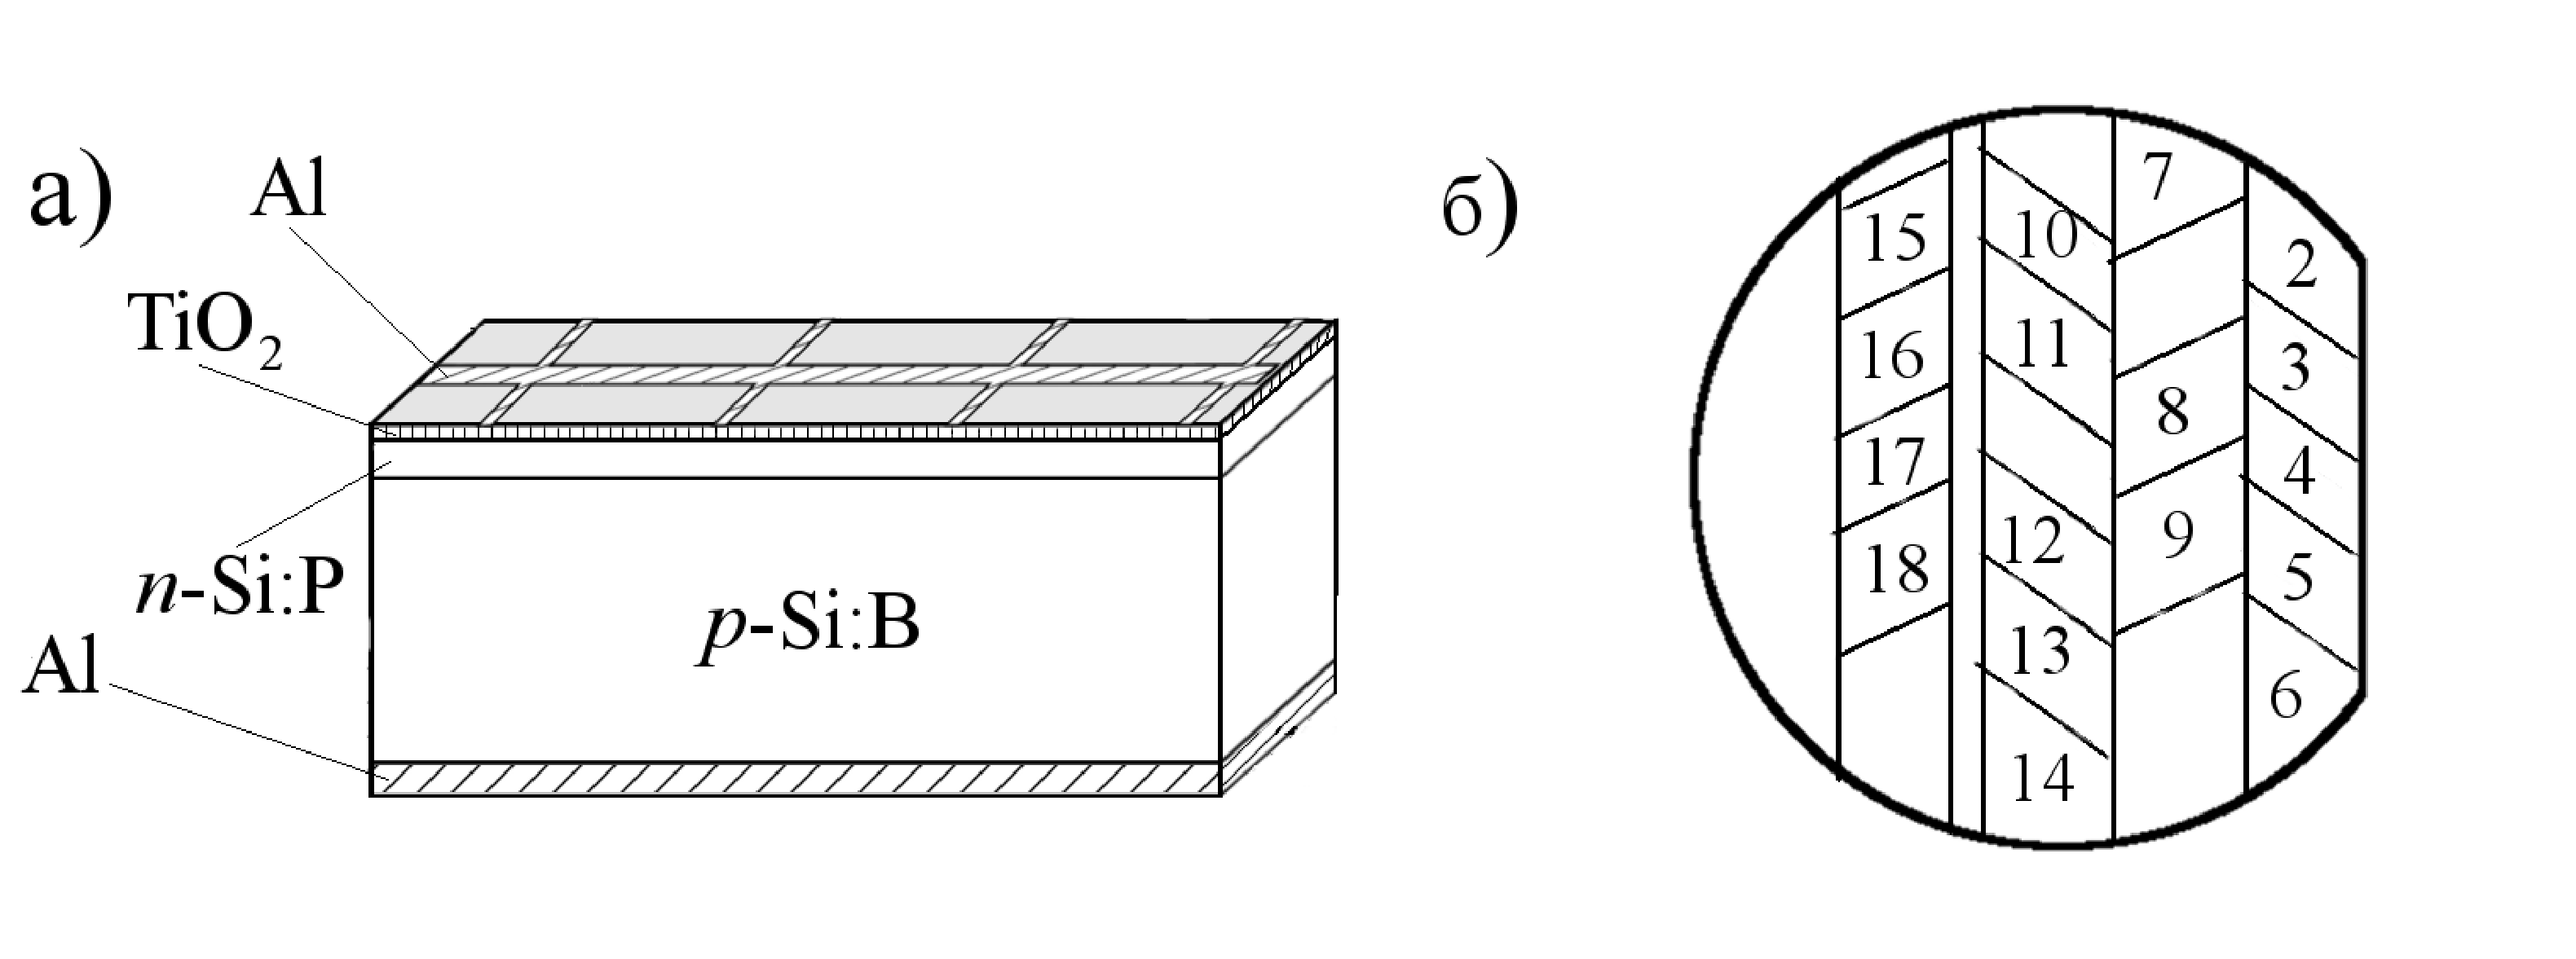
\includegraphics[width=1.0\textwidth]{SSC}%
\caption{\label{figSSC}
Структура кремнієвих сонячних елементів (а) та місце розташування зразків (б).
}
\end{figure}




\chapter{Динамічні акустоіндуковані ефекти в опромінених та неопромінених кремнієвих структурах з p--n переходом\label{Ch_SSC}}
\section{Кремнієві сонячні елементи та режими їх радіаційного опромінення\label{SSC}}
Сонячні елементи, які досліджувалися в роботі, були створені на основі пластин кремнію діаметром близько 100~мм (радіус дорівнював 2 дюйми).
Пластини  були вирізані зі злитків, вирощених за методом Чохральського, мали товщину 300~мкм і були орієнтовані в напрямі $<$111$>$.
Легування здійснювалось шляхом додавання у розплав атомів бору (кремній марки КДБ10).
У дослідженому температурному діапазоні концентрація основних носіїв заряду складала величину $p_p=1,4\cdot10^{15}$~см$^{-3}$.
% та $p_p=4.5\cdot10^{15}$~см$^{-3}$).

Для створення $n^+$ емітера проводилась імплантація іонів фосфору, після закінчення якої було проведено активізуючий відпал.
Як наслідок, був створений шар з електронною провідністю товщиною близько  0,5~мкм з концентрацією вільних носіїв заряду $10^{19}$~см$^{-3}$.

Поверхня пластини була пасивована шляхом нанесення плівки Al$_2$O$_3$.
Крім того, на фронтальну поверхню був нанесений антивідбиваючий шар діоксиду титану (TiO$_2$) з використанням методу APCVD (atmospheric pressure chemical  vapour  deposition).
З використанням методу трафаретного друку (screen printing) було створено омічні алюмінієві електроди (суцільний на задній поверхні та металева сітка на передній).
Нарешті, був проведений швидкий відпал отриманих структур при температурі $800^\circ$C тривалістю декілька хвилин.
Структура досліджених кремнієвих сонячних елементів (КСЕ) зображена на Рис.~\ref{figSSC},а.
Зауважимо, що цей рисунок наведено без збереження масштабних співвідношень між окремими частинами.

Для досліджень використовувалися зразки площею $1,5\div2,1$~cm$^{2}$, вирізані з різних (переважно центральних) областей пластини.
Для позначення зразків надалі використовується запис на кшталт SSC$x$, де $x$ --- номер зразка.
Місце розташування зразків на вихідній пластині показано на Рис.~\ref{figSSC},б.


\begin{figure}
\center
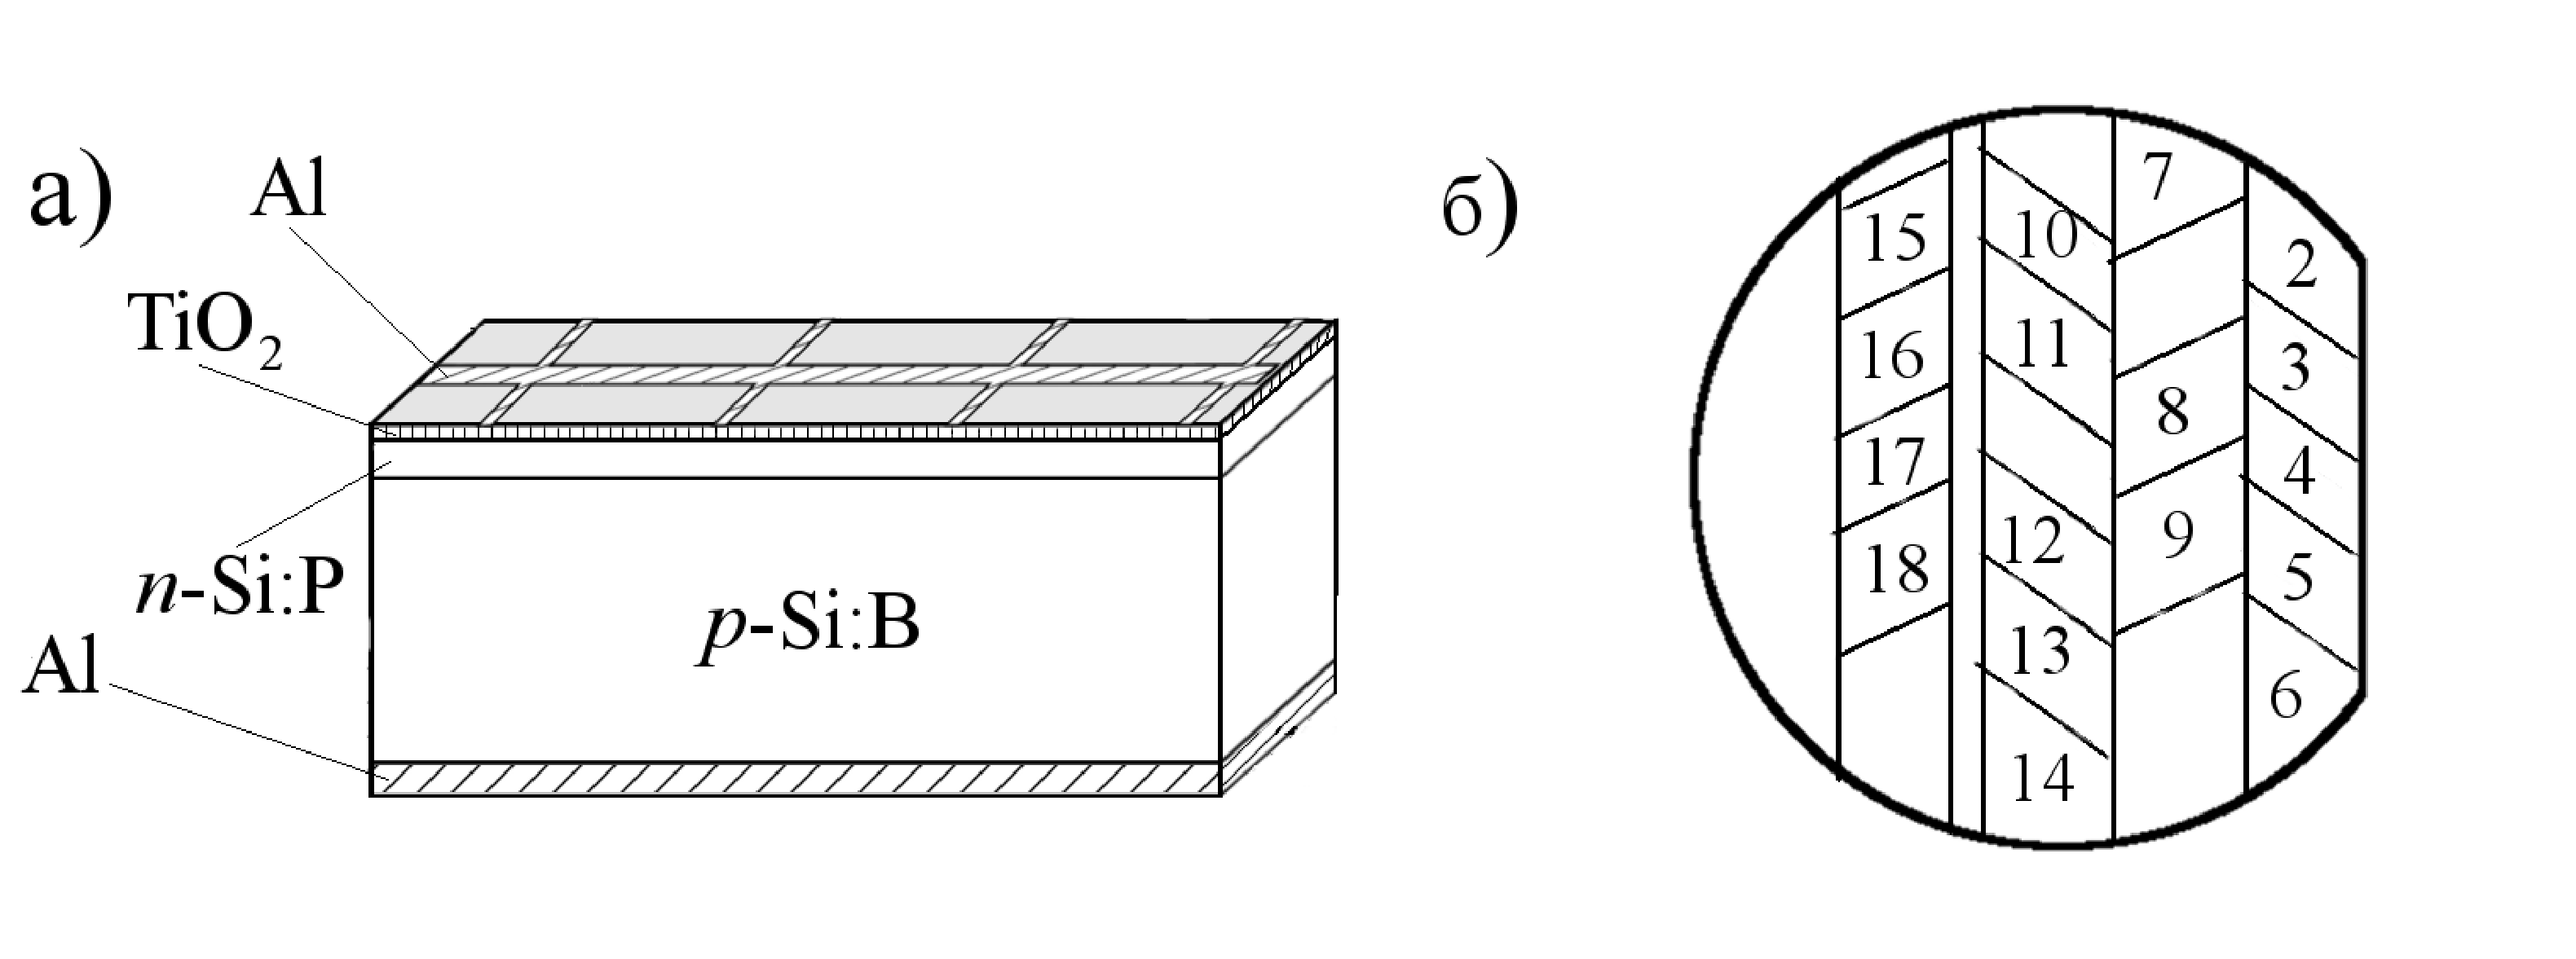
\includegraphics[width=1.0\textwidth]{SSC}%
\caption{\label{figSSC}
Структура кремнієвих сонячних елементів (а) та місце розташування зразків (б).
}
\end{figure}


\begin{table}[b]
\caption{\label{tabSSCSample}Параметри опромінених кремнієвих сонячних елементів.
}
\begin{tabular}{|c|c|c|c|c|c|}
%\begin{tabularx}{\textwidth}{|>{\centering\arraybackslash}X|
%                             >{\centering\arraybackslash}X|
%                            >{\centering\arraybackslash}X|
%                            >{\centering\arraybackslash}X|
%                            >{\centering\arraybackslash}X|
%                            >{\centering\arraybackslash}X|
%                            }
\hline
\multirow{2}{*}{Зразок} &Тип&$D$,&$\Psi$, &NIEL,& $D_d$,  \\
&опромінення& рад& см$^{-2}$&MеВ~см$^2$/г& MеВ/г \\
\hline
nSC4&нейтрони&4,5$\cdot$10$^3$&4$\cdot$10$^{11}$&2,04$\cdot$10$^{-3}$&8,2$\cdot$10$^{8}$\\ \hline
g6SC8&$\gamma$--$^{60}$Co&1$\cdot$10$^6$&1,6$\cdot$10$^{15}$&1,07$\cdot$10$^{-7}$\cite{NIEL:Akkerman}&$(1,7\div2,1)\cdot 10^{8}$\\
\cline{1-4}
\cline{6-6}
g7SC12&$\gamma$--$^{60}$Co&1$\cdot$10$^7$&1,6$\cdot$10$^{16}$&1,31$\cdot$10$^{-7}$\cite{NIEL:Messenger}&$(1,7\div2,1)\cdot 10^9$\\ \hline
\end{tabular}
%\end{tabularx}
\end{table}

Частина зразків, використаних для досліджень, була опромінена або реакторними нейтронами, або гамма--квантами $^{60}$Co.
Флюєнс $\Psi$ нейтронного опромінення складав $4\cdot10^{11}$~см$^{-2}$,
для позначення нейтронно опромінених зразків використовується префікс <<n>> (наприклад <<nSC4>>).
Доза $D$ опромінення гамма-квантами дорівнювала $10^6$ або $10^7$~рад, для позначення відповідних зразків використовуються префікси <<g6>> та <<g7>>, відповідно.

Значення доз та флюєнсів наведено в Таблиці~\ref{tabSSCSample}.
Для визначення кореляцій між $D$ та $\Psi$ для нейтронного та $\gamma-^{60}$Co опромінення використовувалися дані робіт \cite{NIEL:Akkerman,Brauning}.
У цій таблиці також наведено дані щодо величини NIEL (non--ionizing energy losses, енергетичні втрати, не пов'язані з іонізацією) при поширенні нейтронів та гамма--квантів $^{60}$Co в кристалах кремнію.
NIEL характеризує втрати енергії налітаючої частинки на одиницю довжини шляху, пов'язані зі зміщенням атомів ґратки \cite{NIEL:Huhtinen,NIEL:Messenger}, тобто, фактично, процеси радіаційного дефектоутворення.
Зокрема, вважається що радіаційне ушкодження кристалів характеризується такою величиною, як $D_d=\Psi\cdot \mbox{NIEL}$ (displacement damage dose) \cite{NIEL:Messenger}.
Величини $D_d$ для досліджених структур також розміщені у Таблиці~\ref{tabSSCSample}.
З наведених даних видно, що як при використанні нейтронів, так і $\gamma$--квантів очікуване пошкодження кристалічної структури є близьким.
Проте, як відомо,  опромінення різного типу викликає появу різних за структурою дефектів.
Зокрема, $\gamma$--промені викликають появу, переважно, А--центрів \cite{NIEL:Jafari,Gamma:Prabhakara,NIEL:Moll}, тоді як нейтрони призводять до появи вакансійних кластерів\cite{Rew:Srour,Junkes}, областей розупорядкування  \cite{Neutron:Arutyunov} та комплексів C$_i$O$_i$ \cite{NIEL:Moll,neutron:Londos}.
Більш детально це питання розглянуте у розділі~\ref{Rad_SSC}.

Відомо \cite{RadBook}, що після радіаційного опромінення, особливо нейтронного, \cite{NIEL:Moll,Rew:Srour} у кристалах кремнію відбуваються довготривалі перехідні процеси, пов'язані з утворенням вторинних радіаційних дефектів (РД).
Для того, щоб уникнути впливу подібних процесів зразки після опромінення перед початком досліджень, результати який наведено далі, зберігались протягом п'яти років при кімнатній температурі.


Параметри УЗ навантажень КСЕ, їх позначення та зразки, до яких вони застосовувалися, наведено в Таблиці~\ref{tabUSL}.

\begin{table}
\caption{\label{tabUSL}Параметри ультразвукових навантажень КСЕ.
}
%\center
\begin{tabular}{|c|c|c|c|c|c|c|c|}
\hline
$f_\mathtt{US}$,&Тип&$W_{\mathtt{US}}$,&$\xi_{\mathtt{US}}$,&$u_{\mathtt{US}}$,&$T$,&Позначення&Зразок\\
МГц&хвиль&Вт/см$^2$&$10^{-6}$&нм&K&УЗН&\\
\hline
8,0&повздовжні&0,18&1,3&0,3&302$\div$333&U--Ls&SC11, SC17\\ \hline
4,2&поперечні&0,19&2,9&0,63&300$\div$340&U--Ts1&SC17, g7SC12\\ \hline
4,2&поперечні&0,22&3,1&0,67&295$\div$335&U--Ts2&SC11\\ \hline
4,2&поперечні&0,24&3,2&0,70&300$\div$340&U--Ts3&nSC4\\ \hline
4,2&поперечні&0,37&4,0&0,87&308$\div$340&U--Tb1&g7SC12\\ \hline
4,2&поперечні&0,38&4,1&0,89&308$\div$340&U--Tb2&g6SC8\\ \hline
4,2&поперечні&0,40&4,2&0,91&310$\div$340&U--Tb3&SC11, SC17\\
&&&&&&&nSC4\\ \hline
\end{tabular}
\end{table}

\section{Акусто--керована деградація кристалічних кремнієвих сонячних елементів\label{USID}}

На сьогодні КСЕ продовжують відігравати домінуючу роль у галузі фотовольтаїки.
Основними причинами є достатньо високий рівень коефіцієнта корисної дії, низька ціна та високий рівень розвитку технологічних процесів, необхідних для їх виготовлення.
Першочерговою задачею виробників КСЕ (як і інших напівпровідникових пристроїв) є можливість керування їх властивостями,
що, насамперед, пов'язане з розумінням причинно--наслідкових зв'язків процесів, які відбуваються під час фотогенерації та руху носіїв заряду.
Наприклад, виявлено, що зменшення ефективності роботи КСЕ може відбуватися внаслідок
\begin{enumerate}[label=\asbuk*),leftmargin=0em,itemindent=1.5em]
  \item інтенсивного освітлення --- процес, який у випадку СЕ на основі кристалічного кремнію носить назву LID (light--induced degradation) \cite{LID:SchmidtJMR,LIDRev,LIDRev2,LID:JAP2017II}, тоді як для мікрокристалічного Si широко використовується абревіатура CID (carrier-induced degradation) \cite{CID:APL,CID:PPS};
  \item прикладання високої (декілька сотень вольт і більше) напруги --- PID  (potential--induced degradation) \cite{PID:SEMSC,PID:PP,PID:2017};
  \item радіаційного опромінення ---  RID (radiation--induced degradation) \cite{Bhat,Karazhanov}.
\end{enumerate}
Причинами деградації є зміни у дефектній підсистемі кристалів.
Це може бути перебудова комплексів бор--кисень або комплексів, які містять мідь (для випадку LID),
декорування дефектів пакування позитивно зарядженими іонами, переважно, натрію, що спричинює зменшення шунтуючого опору (PID)
або утворення радіаційних рекомбінаційних центрів (RID).
Відпал деградованих КСЕ при підвищених температурах нерідко дозволяє повністю (або частково) відновити ефективність.

В той же час, УЗ також здатний ефективно взаємодіяти з дефектами в кремнії.
Наприклад, було експериментально показано що УЗ викликає трансформацію домішкових та радіаційних дефектів \cite{Korotchenkov1995,Ostapenko1995,UST:Medvid,YOlikh:SupMicr},
модифікацію спектру \cite{Zaver:2008} та густини \cite{Mirsagatov} поверхневих станів,
зміну дифузійної довжини електронів \cite{Ostapenko1999,Ostrovskii2001}
та впливає на проходження струму у бар'єрних структурах \cite{Davletova2009,Davletova2008,YOlikh2005}.
Детальніше ці ефекти описані в розділі~\ref{Oglyad}.
Тобто, цілком очікуваним є те, що внаслідок поширення АХ в КСЕ може виникати ефект акусто--індукованої деградації (USID, ultrasound--induced degradation).
При використанні УЗ не надто високої інтенсивності, параметри матеріалу після припинення поширення АХ повертаються до вихідних значень \cite{Ostapenko1999,Ostrovskii2001,Korotchenkov1995} навіть без застосування відпалу.
Тому очікується, що USID має бути оборотною при кімнатних температурах на відміну від деградацій інших типів.
Представлені у даному параграфі результати отримані в результаті експериментального дослідження АІ змін фото--електричних параметрів КСЕ.

\subsection{Особливості визначення параметрів КСЕ}
Для визначення параметрів КСЕ проводилось вимірювання прямих ділянок ВАХ зразків у темряві та при освітленні.
Вимірювання проводились в температурному інтервалі  290--340~K як за умов УЗН, так і без нього.
Як приклад, декілька отриманих кривих наведено на Рис.~\ref{figSSCIV}.

\begin{figure}
\center
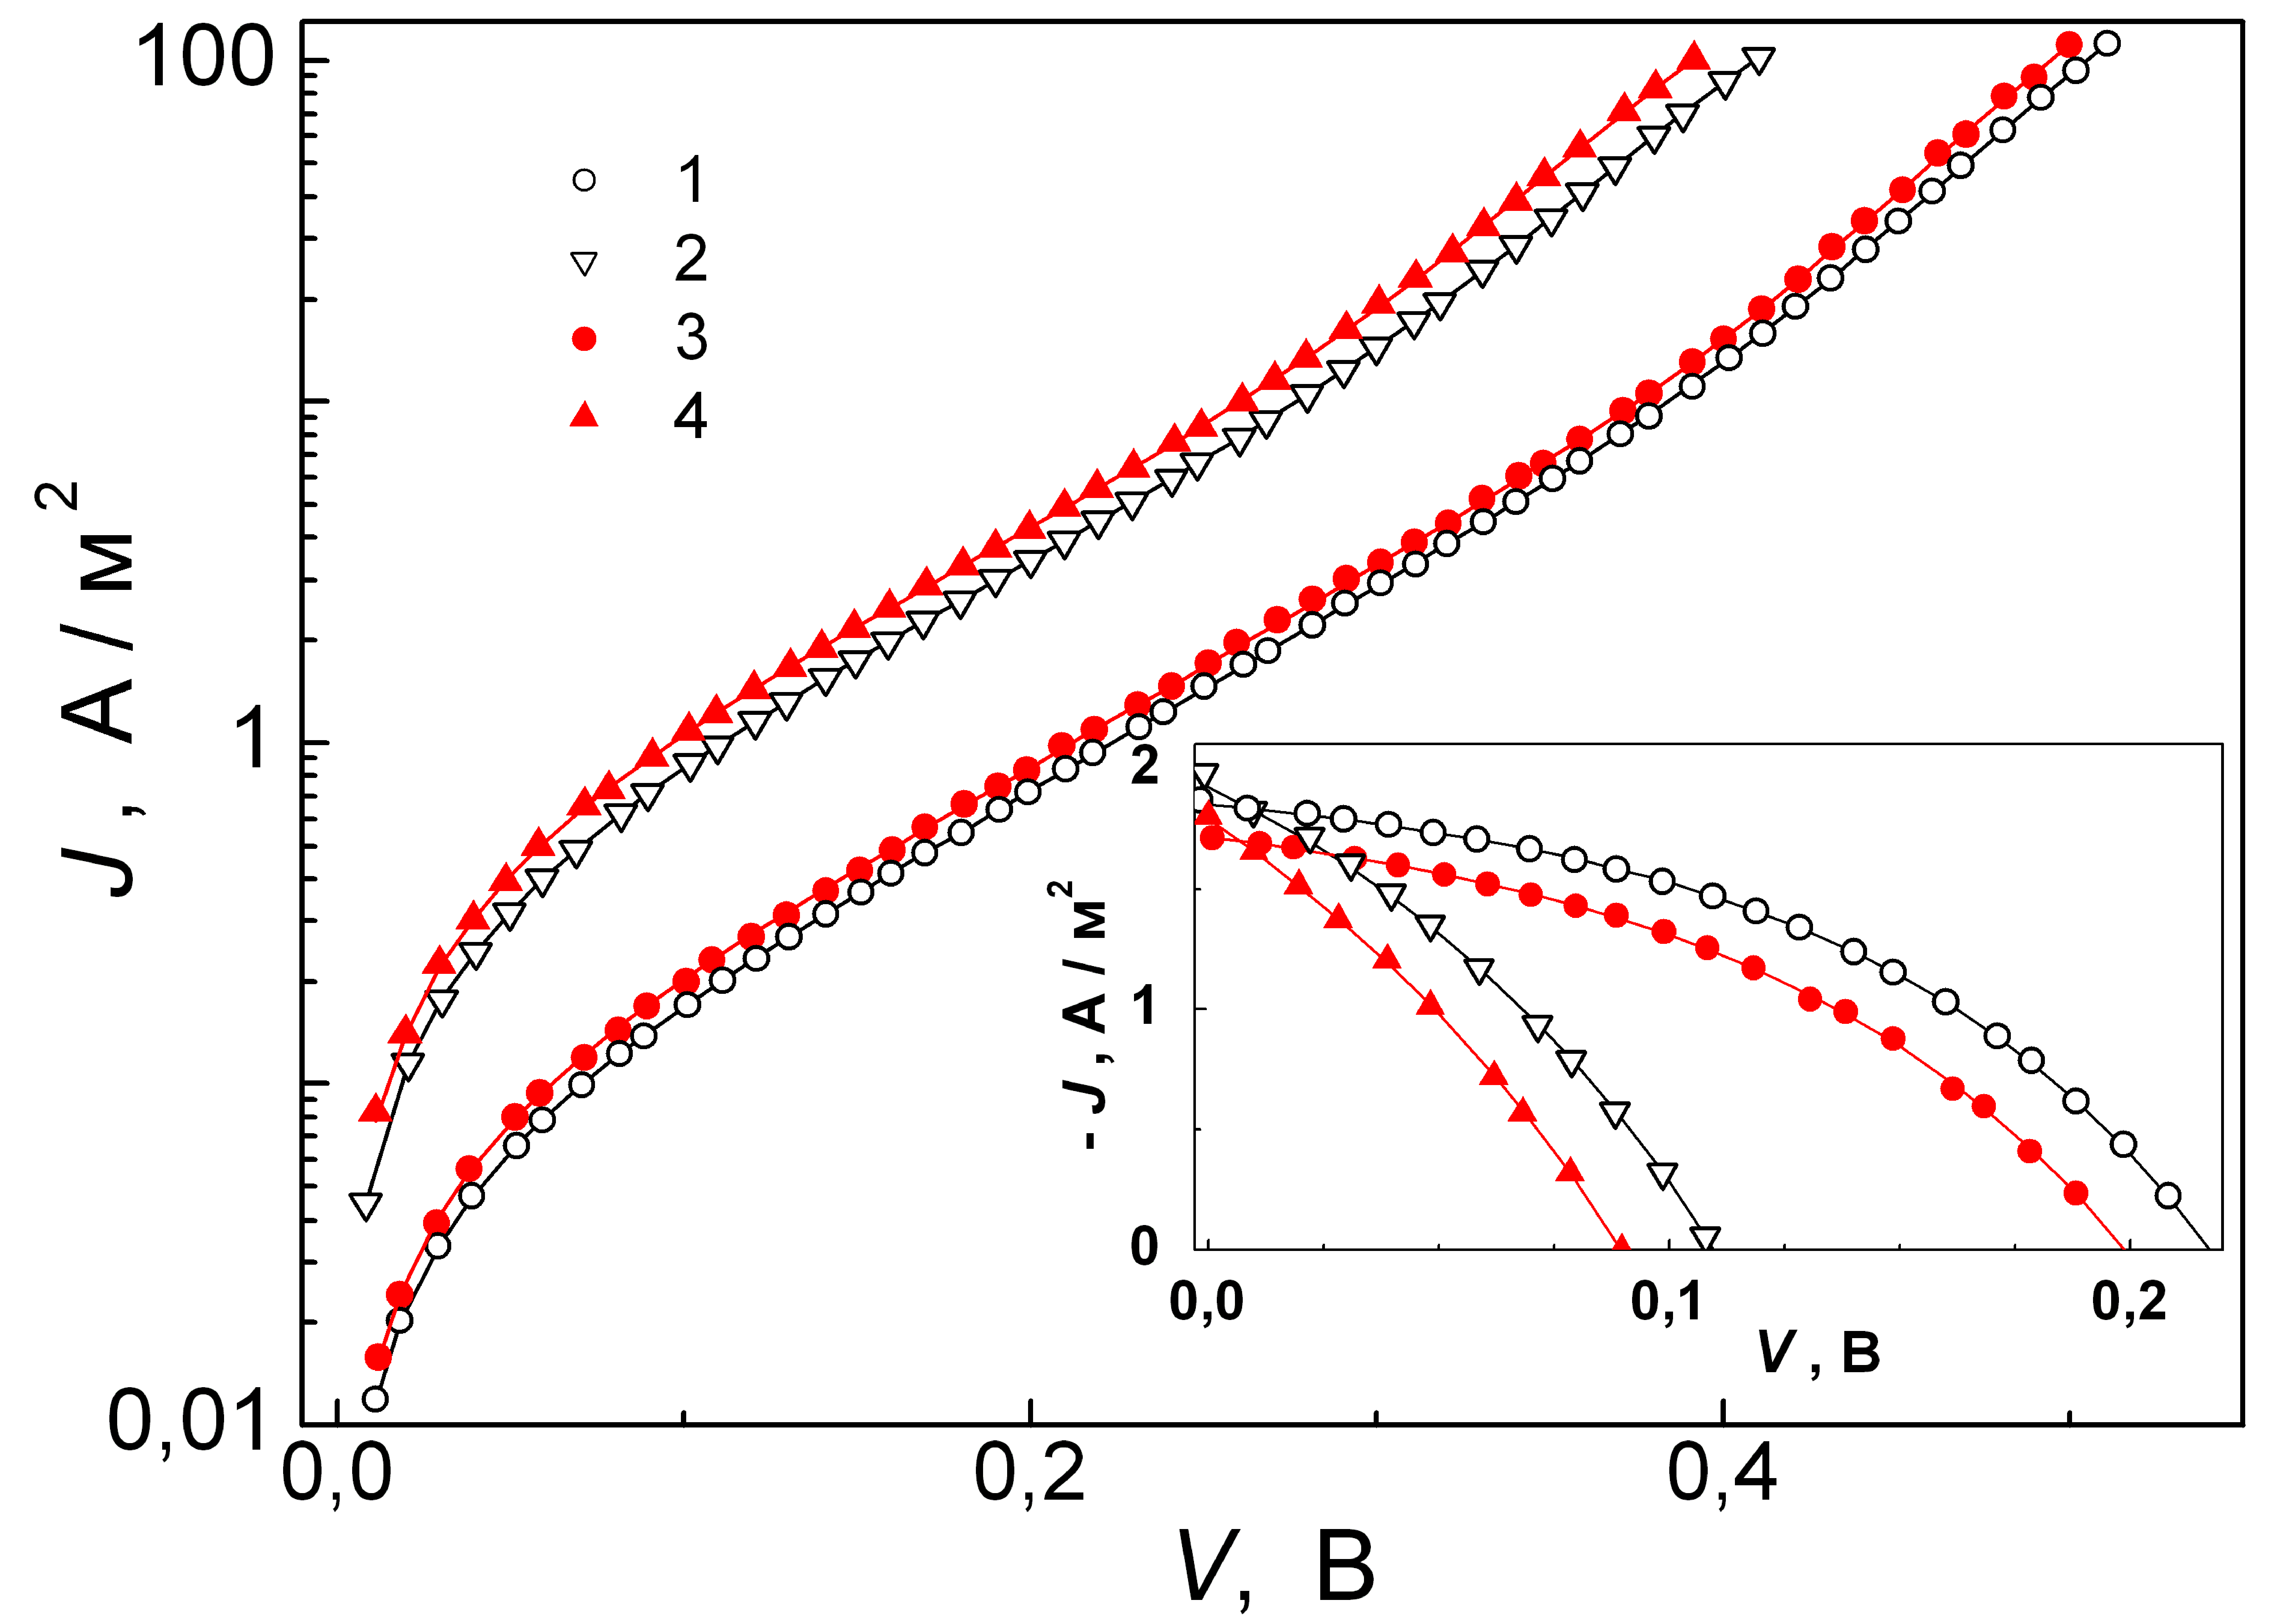
\includegraphics[width=0.9\textwidth]{figSSCIV}%
\caption{\label{figSSCIV}
Темнові ВАХ, виміряні при температурах 301~K (криві 1 та 2, кола) та 341~K (криві 2 та 4, трикутники)
за умов УЗН (U--Tb3, криві 2, 4, заповнені символи) та для ненавантаженого зразка (криві 1 та 3, порожні символи)
На вставці наведено частину ВАХ при освітлені в діапазоні прямих зміщень від 0 до $V_{oc}$.
Символи відображають результати вимірів, лінії отримані шляхом апроксимації за формулами (\ref{eqSSCIV}) та (\ref{eqW}).
%(\labelcref{eqSSCIV,eqW}) \ref{eqW}.
}%
\end{figure}

Густина струму короткого замикання $J_{sc}$, напруга холостого ходу $V_{oc}$ та фактор форми $F\!F$ визначалися з ВАХ, отриманих при освітленні, 
традиційним способом за перетином експериментальної кривої з координатними осями  та по розташуванню максимуму потужності.

В рамках моделі подвійного діоду залежність густини струму $J$ від прикладеної напруги $V$ для  n$^+$--p сонячного елементу має описуватися наступним виразом:

\begin{eqnarray}
\label{eqSSCIV}
\nonumber J(V,\,T)&=&-J_{ph}+\frac{qn_id}{2\tau_{g}}\left\{\exp \left[\frac{q(V-JR_s)}{n_\mathrm{id}kT}\right]-1\right\}+\\
&&+\frac{qn_i^2}{p_p}\sqrt{\frac{\mu_nkT}{\tau_n}}\left\{\exp \left[\frac{q(V-JR_s)}{kT}\right]-1\right\}+\frac{V-JR_s}{R_{sh}}\,,
\end{eqnarray}
де
$T$ --- абсолютна температура,
$J_{ph}$ --- густина фотогенерованого струму,
$q$ --- елементарний заряд,
$n_i$ --- концентрація власних носіїв заряду,
$\tau_{g}$  --- ефективний час життя носіїв заряду в області просторового заряду (ОПЗ),
$d$ --- товщина ОПЗ:
\begin{equation}
\label{eqW}
    d(V,\,T)=\sqrt{\frac{2 \varepsilon \varepsilon_0(p_p+n_n)}{q p_p n_n}\left[\frac{E_g}{q}-\frac{kT}{q}\ln\left(\frac{N_vN_c}{p_pn_n}\right)-\frac{2kT}{q}-V\right]} \,,
\end{equation}
$\varepsilon_0$ --- діелектрична стала,
$\varepsilon$ --- діелектрична проникність матеріалу (для Si $\varepsilon=11,7$),
$p_p$ та $n_n$ --- концентрація основних носіїв заряду в $p$-- та $n$--області, відповідно;
$E_g$ --- ширина забороненої зони напівпровідника,
$N_c$ та $N_v$ --- ефективна густина станів поблизу дна зони провідності та вершини валентної зони, відповідно;
$n_\mathrm{id}$ --- фактор неідеальності
$R_s$ та $R_{sh}$ --- послідовний та шунтуючий опори, відповідно;
$\mu_n$ та $\tau_n$ --- рухливість та час життя електронів (неосновних носіїв) в базі діоду.
Рівняння ВАХ, яке моделює поведінку сонячного елементу за допомогою еквівалентної електричної схеми,
містить ряд параметрів, що безпосередньо стосуються фізичних процесів, які відбуваються у пристрої.
Зокрема вважається, що 
$J_{0base}=(qn_i^2/n_n)\sqrt{\mu_nkT/\tau_n}$ пов'язане з процесами рекомбінації у квазі--нейтральній області,тоді як
$J_{0SCR}=(qdn_i/2\tau_{g})$ описує загальну рекомбінацію в ОПЗ.

Формули (\ref{eqSSCIV})--(\ref{eqW}) були використані для апроксимації експериментальних даних, причому
невідомими величинами вважалися $\tau_g$, $\tau_n$, $n_{\mathrm{id}}$, $R_{sh}$, $R_s$ та  $J_{ph}$ (остання лише для ВАХ при освітленні).
При цьому вважалося, що
$n_i(T)=1,64\cdot10^{15}\,T^{1,706}\exp(-E_g/2kT)$~см$^{-3}$ \cite{ni:Green}, $N_c(T)=2,86\cdot10^{19}(T/300)^{1,58}$~см$^{-3}$, $N_v(T)=3,10\cdot10^{19}(T/300)^{1,85}$~см$^{-3}$
\cite{Nc:Green},
а температурні залежності забороненої зони та рухливості електронів описуються формулами Varshni та Caughey--Thomas, відповідно:
\begin{equation}
\label{eqEg}
 E_g(T) = E_g(0) - \frac{\beta_1 T^2}{(T + \beta_2)}\,,
\end{equation}
де 
$E_g(0)=1,169$~еВ,
$\beta_1=7,021\cdot10^{-4}$~еВ/К$^2$,
$\beta_2=1108$~K \cite{Schroder2006,Markvart} та
\begin{equation}
\label{eqMu}
\mu_n(T) = \mu_{min}+\frac{\mu_0}{1+(p_p/N_{ref})^{\zeta}}\,.
\end{equation}
де
$\mu_{min}=92\cdot(T/300)^{-0,57}$~см$^2$/(В$\cdot$с), 
$\mu_0=1268\cdot(T/300)^{-2,33}$~см$^2$/(В$\cdot$с), 
$N_{ref}=1,3\cdot10^{17}\cdot(T/300)^{2,4}$~см$^{-3}$,
$\zeta=0,91\cdot(T/300)^{-0,146}$ \cite[с.~505, Table~A8.2]{Schroder2006}.
Апроксимація проводилась з використанням методу диференційної еволюції\cite{DE:Sun,DEWang,DEModif}, який більш детально описано в параграфі~\ref{subEA}.
Приклади результуючих апроксимуючих кривих наведено  на Рис.~\ref{figSSCIV}.
Видно, що вони досить добре апроксимують експериментальні дані.

Відомо, що $J_{sc}\approx J_{ph}R_{sh}/(R_{sh}+R_{s})$.
Для всіх досліджених зразків величина $R_s$ приблизно дорівнювала 2~Ом$\cdot$см$^2$, тоді як значення $R_{sh}$ суттєво залежала від температури та конкретного зразка, проте для
розглянутого температурного інтервалу не було меншим  4~кОм$\cdot$см$^2$.
Отже, очікується, що в нашому випадку має бути $J_{sc}\approx J_{ph}$.
І дійсно, подібне співвідношення спостерігається між величиною $J_{ph}$, отриманою шляхом багатопараметричної апроксимації
повної залежності густини струму від напруги, та значенням $J_{sc}$, яке відображає ординату перетину ВАХ з віссю струмів. 

Для освітлення КСЕ використовувалося монохроматичне (довжина хвилі $\lambda=900$~нм) світло з низькою інтенсивністю.
Відомо \cite{BO:Halam2016}, що освітлення з інтенсивністю вище 0.01~suns може викликати в кремнії р--типу утворення дефектів.
Так як метою роботи було дослідження АІ ефектів, то з метою запобігання будь--яких світло--індукованих деградаційних процесів було використане 
освітлення з інтенсивністю $W_{ph}=(8\pm4)$~Вт/м$^2$.
Монохроматичність світла дозволила спростити аналіз причин АІ змін струму короткого замикання.
А саме, для використаної довжини хвилі фотогенерований струм пов'язаний, переважно, з утворенням електронно--діркових пар в $p$--області.
У випадку, якщо база СКЕ перевищує у декілька разів довжину дифузії неосновних носіїв $L_n=\sqrt{\mu_nkT\tau_n/q}$, то
для $J_{sc}$ справедливий вираз \cite{Markvart,Razeghi}:
\begin{equation}
\label{eqIph}
J_{sc} = \frac{W_{ph}(1-M)q\beta\lambda}{hc}\frac{\alpha L_n}{1+ \alpha L_n}\,,
\end{equation}
де
$\alpha$ --- коефіцієнт поглинання світла,
$M$ --- коефіцієнт відбивання,
$\beta$ --- коефіцієнт квантового виходу.

Формулу~(\ref{eqIph}) було використано для апроксимації експериментальної залежності $J_{sc}(T)$,
при чому $L_n$ розглядалась як невідомий параметр.
Під час розрахунків вважалося, що $\beta$ та $M$ не змінюються, а
температурна залежність $\alpha$ описується виразом \cite{Markvart,Si:Absorb}
\begin{eqnarray}
\label{eqAlpha}
\nonumber \alpha(\lambda,\,T)&=&\sum_{\substack{i=1,2\\j=1,2}}\!C_iA_j\left\{\frac{[hc/\lambda-E_{gj}(T)+E_{p\,i}]^2}{\exp(E_{p\,i}/kT)-1}\:+
\frac{[hc/\lambda-E_{gj}(T)-E_{p\,i}]^2}{1-\exp(-E_{p\,i}/kT)}\right\}+\\
&&+A_d\left[hc/\lambda-E_{gd}(T)\right]^{1/2}\,,
\end{eqnarray}
де 
$h$ --- стала Планка,
$c$ --- швидкість світла,
$E_{p\,1}=1,827\cdot10^{-2}$~еВ,
$E_{p\,2}=5,773\cdot10^{-2}$~еВ --- частоти Дебая поперечних
оптичних та акустичних фононів, відповідно; 
константи $C_1=5,5$, 
$C_2=4,0$, 
$A_1=3,231\cdot10^2$~см$^{-1}$еВ$^{-2}$,
$A_2=7,237\cdot10^3$ см$^{-1}$еВ$^{-2}$,
$A_d=1,052\cdot10^6$ см$^{-1}$еВ$^{-2}$; 
температурна залежність $E_{g1}$, $E_{g2}$ та $E_{gd}$ описується виразом \ref{eqEg}),
причому $E_{g1}(0)=1,169$~еВ, $E_{g2}(0)=2,5$~еВ та $E_{gd}(0)=3,2$~еВ.
Крім того, припускалося що $L_n\sim T^{0.5}$.
Основою для цього були результати, отримані при апроксимації окремих ВАХ (детальніше див. параграф~\ref{sbQNR}).

Таким чином, визначення $L_n$ та $\tau_n$ проводилось як в результаті аналізу окремої ВАХ, так і з апроксимації 
температурної залежності $J_{sc}$.
Надалі, щоб відрізнити величини, отримані другим шляхом, використовується верхній індекс <<$ph$>>: $L_n^{ph}$, $\tau_n^{ph}$, $\varepsilon_{\tau n}^{ph}$ тощо.

%We would like to stress that, firstly, all found AI effects are reversible.
%In other word, the $J_{sc}$, $V_{oc}$, $F\!F$, and another parameters, which are described above, revert to the initial value
%after the UL termination and sample storage for about 24~h at room temperature.
%The reversibility testifies that ultrasound neither causes defect diffusion nor changes defect concentration.
%Secondly, the AI relative changes are weakly depend on temperature over the explored range.

%Fig.~\ref{fig_Reverse} illustrates the reversibility of AI effects.
%The time interval between USL initiation and "during" measurement was longer than 60~min,
%and the time interval between USL termination and "after" measurement was about 24~h.
%The data for nSC and g6SC are similar to those presented for iSC and g7SC.
%
%
%
%\begin{figure*}
%\includegraphics[width=0.7\textwidth]{fig_2ab}%
%\caption{\label{fig_Reverse}
%SCR lifetime (a, left axis, open marks),
%base lifetime (a, right axis, filled marks),
%ideality factor (b, left axis, open marks), and
%shunt resistance (b, right axis, filled marks)
%obtained before, during, and after USL at 330~K.
%Data for iSC (circles) and g7SC (triangles) are presented.
%}%
%\end{figure*}


Зауважимо, що величини параметрів ($\tau_g$, $\tau_n$, $n_{\mathrm{id}}$, $R_{sh}$ та $R_s$) отримані з ВАХ, які виміряні у темряві та при освітленні за однакової температури
та в ідентичних умовах УЗН, практично співпадають.

\subsection{АІ вплив на рекомбінаційні процеси у квазі--нейтральній області\label{sbQNR}}

\section{Особливості акусто--дефектної взаємодії в опромінених кремнієвих структурах з p--n переходом\label{Rad_SSC}}

\section*{Висновки до розділу \ref{Ch_SSC}}
\addcontentsline{toc}{section}{Висновки до розділу \ref{Ch_SSC}}
  \begin{enumerate}
     \item Проведено
  \end{enumerate}	

Основні результати даного розділу представлені в роботах \cite{Olikh:Rev,6CPFCS}.



\chapter{\MakeUppercase{Порівняльний аналіз та оптимізація методів розрахунку параметрів структур метал---напівпровідник}\label{Ch_MSMethod}}


\section{Основні параметри діодів Шотткі}
Напівпровідникові бар'єрні структури, як вже зазначалося раніше, широко застосовуються у техніці.
Визначення параметрів подібних структур відіграє надзвичайну важливу роль під час розробки, проектування та виготовлення пристроїв.
%Параметри подібних структур є найбільш суттєвим фактором для можливості практичного використання,
%а їх відіграє надзвичайну важливу роль під час розробки, проектування та виготовлення пристроїв.
Один із найпроширеніших шляхів визначення параметрів полягає у вимірюванні ВАХ.
При цьому взаємозв'язок між струмом та напругою описується за допомогою певних фізичних моделей, у
результаті чого виникає можливість вичленити параметри, спираючись на результати експериментальних вимірювань.
Наприклад, пряма гілка ВАХ діодів Шотткі (ДШ) згідно з моделлю термоемісії має описуватися \cite{Rhoderick1988} наступними виразами
\begin{eqnarray}
\label{eqSDIV}
I&=&I_s\left\{\exp\left[\frac{q(V-IR_s)}{n_\mathrm{id}kT}\right]-1\right\}\,,\\
\label{eqSDIs}
I_s&=&AA^*\,T^2\exp\left(-\frac{q\Phi_b}{kT}\right)\,,
\end{eqnarray}
де
$I_s$ --- струм насичення,
%$q$ --- елементарний заряд,
$R_s$ --- послідовний опір,
$n_\mathrm{id}$ --- фактор неідеальності,
%$k$ --- стала Больцмана,
%$T$ --- абсолютна температура,
%$A$ --- площа діода,
$A^*$ --- ефективна стала Річардсона,
$\Phi_b$ --- висота бар'єру Шотткі (ВБШ) при нульовому зміщенні.
$\Phi_b$ (або $I_s$), $n_\mathrm{id}$ та $R_s$ є найфундаментальнішими параметрами цієї моделі та повинні бути максимально точно визначені з експериментальних ВАХ.
У літературі запропоновано чимало методів визначення параметрів ДШ.
Найпростіший стандартний метод вимагає наявності лінійної області на залежності $\ln(I)$ від  $V$ \cite{Sze2012,Rhoderick1988}.
При цьому два параметри, $n_\mathrm{id}$ та $\Phi_b$, можуть бути визначені за кутом нахилу та перетином  залежності з віссю струмів, відповідно.
На жаль, подібний підхід перестає бути дієздатним у випадку, коли структура характеризується значним послідовним опором.
Зокрема, рівняння~(\ref{eqSDIV}) є трансцендентним, що суттєво ускладнює математичні аспекти визначення параметрів.
З одного боку, існує цілий набір аналітичних методів екстракції параметрів ДШ.
%Зважаючи на складність задачі, існує цілий ряд методів, які вирішують задачу екстраполяції параметрів ДШ.
Вони базуються на безпосередніх алгебраїчних наближеннях і використовують різноманітні допоміжні функції \cite{Norde,Lien,Werner,Cheung,Gromov,Lee,Bohlin,Cibils,Manifacier},
процедури  диференцювання  \cite{Mikhelashvili} або інтегрування  \cite{Kaminski,Ortiz1995,Durmus} ВАХ,
розбиття діапазону напруг на декілька частин \cite{Cataldo},
вимірювання ВАХ при декількох температурах \cite{Sato} або з використанням додаткового зовнішнього опору \cite{Lyakas}.


З іншого боку, визначення параметрів є багатовимірною задачею оптимізації і тому для її вирішення запропоновано різноманітні числові методи \cite{Ortiz1999,Evangelou,Donoval,Ferhat}.
Зазвичай, вони використовують метод найшвидшого градієнтного спуску для мінімізації різниці між виміряними та апроксимуючими значеннями.
Окремі автори\cite{Lambert_Jung,Ortiz2005} шукають розв'язок рівняння~(\ref{eqSDIV}) використовуючи $W$--функцію Ламберта
\cite{LambertBook}.
Зазвичай, числові методи характеризуються вищим рівнем достовірності визначення параметрів, проте нерідко вимагають відносно тривалих розрахунків.
Крім того, нерідко спостерігається тенденція збіжності у локальний екстремум замість глобального.

Нарешті, порівняно нещодавно запропоновано використовувати еволюційні алгоритми (ЕА) для визначення параметрів напівпровідникових пристроїв \cite{PSO_Ye,DEWang,GA_Li,P-DE_Ishaque,TLBO_Patel,MABC,PSOWang,GA_Schottky}.
Це стохастичні методи, які виявляють надзвичайно високу ефективність при оптимізації дійсних цільових функцій багатьох змінних.
На відміну від числових методів, ЕА може бути застосований до нелінійних функцій без необхідності розрахунку похідних, а також слабко залежить від початкових наближень значень параметрів.
ЕА вважаються \cite{P-DE_Ishaque} найобіцяючими  методами розрахунку параметрів.

Про важливість задачі визначення параметрів ДШ свідчить хоча б той факт, що
незважаючи на досить тривалу історію вивчення питання та накопичений достатньо широкий асортимент методів вирішення цього завдання,
у літературі постійно з'являються пропозиції щодо нових варіантів методів.
Наприклад, серед подібних робіт лише у другій половині 2017~року можна виділити \cite{Noise:Roy,MikhelashviliJAP2017,Cataldo,ORTIZCONDE2018}.

У літературі наявні роботи \cite{Evangelou,Aubry,Kudryk}, в яких проводиться порівняння  та огляд шляхів визначення параметрів ДШ, проте вони переважно зосереджені на розгляді лише декількох метод і фактично не беруть до уваги еволюційні алгоритми.
Задача, яка вирішувалась під час досліджень, описаних у цьому розділі, полягала у порівнянні ефективності (точності визначення параметрів та швидкості роботи) різних методів визначення параметрів структур метал---напівпровідник (МН) із ВАХ.
Крім того, розглянуто питання впливу величини окремих параметрів на точність визначення всього набору.
Використані лише методи, які дозволяють визначити $\Phi_b$, $n_\mathrm{id}$ та $R_s$ використовуючи лише одну ВАХ.
Зокрема, увага сфокусована на 10 аналітичних методах, 2 числові методах та 4 еволюційних алгоритмах
(диференційної еволюції (DE, differential evolution),
оптимізації зграї частинок (PSO, particle swarm optimization),
модифікованої штучної бджолиної сім'ї (MABC, modified artificial bee colony) та
оптимізованого викладання та навчання (TLBO, teaching learning based optimization)).


%Основні результати даного розділу представлені в роботах \cite{Olikh:Rev,6CPFCS}.

\section{Контрольні вольт--амперні характеристики}
Досліджені методи були застосовані до наборів ВАХ, отриманих як експериментально, так і синтезованих штучно.
В останньому випадку використовувалися як ідеальні характеристики, так і криві з певним рівнем шуму, який віддзеркалював можливість наявності випадкових похибок вимірювань у реальних умовах.

\subsection{Ідеальні синтезовані ВАХ\label{SubData}}
Переважно, для оцінки спроможності визначення параметрів структур МН за допомогою аналітичних \cite{Norde,Lien,Werner,Gromov,Lee,Bohlin,Cibils,Mikhelashvili,Kaminski} та числових \cite{Evangelou,Donoval} методів, а також еволюційних алгоритмів \cite{PSO_Ye,P-DE_Ishaque,TLBO_Patel} використовують структури на основі кремнію.
Керуючись таким загальноприйнятим підходом, під час синтезу ВАХ вважалося, що використовується кремнієвий ДШ.
ВАХ були розраховані за допомогою рівняння ~(\ref{eqSDIV}), для розв'язку якого застосовувався метод дихотомії \cite[с.~158]{KalitkinBook}.
При цьому використовувалися значення $A=3,14\cdot10^{-6}$~м$^2$ та $A^*=112$~A$\,$cм$^{-2}$K$^{-2}$ (випадок $n$--Si \cite{Schroder2006}).
Напруга змінювалась із кроком 0,01~В, струм вар'ювався в діапазоні $10^{-9}\div10^{-2}$~A.

Задача полягала у перевірці ефективності методів при різних значеннях параметрів і тому дані були синтезовані для діапазону температур від 130 до 330~К.
Водночас, були синтезовані ВАХ, які близькі до характеристик реальних діодів.
Тому температурні залежності $\Phi_b$, $n_\mathrm{id}$ та $R_s$ обрані, використовуючи наступні міркування.
Як передбачено теорією \cite{Rhoderick1988} та спостережено на експерименті \cite{Aboelfotoh,Zhua},
для випадку однорідного контакту  ВБШ має зменшуватись із підвищенням температури, причому очікувана залежність подібна до температурної залежності ширини забороненої зони напівпровідника.
Тому для апроксимації температурної залежності ВБШ використовувалося рівняння Варшні \cite{SiEg2012}
\begin{equation}
\label{eqFbT}
\Phi_b(T) = \Phi_b(0) - \frac{7,021\cdot10^{-4} T^2}{T + 1108} ,
\end{equation}
причому вважалося, що ВБШ при нульовій температури $\Phi_b(0)=0,75$~еВ.
Температурна залежність фактора неідеальності нерідко описується співвідношенням
\begin{equation}
\label{eqnT}
n_\mathrm{id}=1+\frac{T_0}{T},
\end{equation}
де величина константи $T_0$ для кремнію перебуває в діапазоні $20\div50$~K \cite{T0:Lee,T0:McCafferty,T0:Saxena,Aboelfotoh}.
Для синтезу ВАХ використане значення $T_0=35$~K.
Температурна залежність послідовного опору може бути описана виразом \cite{Sze2012,Rs:Meyaard,Rs:Kang}
\begin{equation}
\label{eqRsT}
R_s=R_{s0}\exp\left(\frac{E_a}{kT}\right),
\end{equation}
де $E_a$ -- енергія активації легуючої домішки.
Були використані значення $E_a=0,044$~еВ (що відповідає домішковому атому фосфору) та $R_{s0}=0.25$~Ом.

Як наслідок, набір синтезованих для аналізу ВАХ складався з 21 кривої, які відповідали інтервалу температур $130\div330$~К із кроком 10~К.
При цьому  $\Phi_b$, $n_\mathrm{id}$ та $R_s$ змінювалися від 0,740 до 0,697~еВ, від 1,27 до 1,11 та від 12,6 to 1,2~Ом, відповідно.


\subsection{Синтезовані ВАХ із випадковими похибками}
З метою аналізу стійкості методів визначення параметрів до наявності випадкових похибок, які виникають під час вимірювань,
%моделювання можливих випадкових похибок, які виникають під час вимірювань, та аналізу стійкості методів визначення параметрів до їх,
також були синтезовані набори ВАХ, в яких значення напруги та струму вибиралися з певним рівнем шуму.
При цьому напруга $V_i$ та струм $I_i$, які відповідали $i-$й точці ВАХ вибиралися випадковим чином використовуючи розподіл Гауса.
Тобто густина ймовірності очікування певної величини напруги описувалася виразом
\begin{equation}
\label{eqGaus}
f(V_i,\overline{V}_i,\sigma_V)=\frac{1}{\sigma_V\sqrt{2\pi}}\exp\left[-\frac{(V_i-\overline{V}_i)^2}{2\sigma_V^2}\right].
\end{equation}
При цьому середнє значення (сподівання) напруги $\overline{V}_i$ змінювалося з кроком 0,01~В,
середнє значення сили струму $\overline{I}_i$ обчислювалося використовуючи рівняння~(\ref{eqSDIV}) та $\overline{V}_i$.
Стандартне відхилення (дисперсія) напруги $\sigma_V$ вибиралася сталою для всього набору (21 криві) ВАХ.
Водночас стандартне відхилення сили струму $\sigma_I$ залежало від абсолютної величини сили струму $\sigma_I=\sigma_I^\varepsilon\cdot\overline{I}_i$,
де постійної для всього набору ВАХ була величина $\sigma_I^\varepsilon$ --- відносна дисперсія струму.
Такий підхід відповідає достатньо поширеному на практиці випадку, коли відносні похибки вимірювання напруги та струму залишаються сталими для всієї ВАХ.
Надалі для позначення синтезованих подібним чином ВАХ буде використовуватися термін "зашумлені синтезовані дані" (noisy synthetic data).

Різні набори синтезованих ВАХ відрізнялися значеннями $\sigma_V$ та $\sigma_I^\varepsilon$.
Фактично, для ідеальних синтезованих ВАХ $\sigma_V=0$~В та $\sigma_I^\varepsilon=0$.


\subsection{Експериментальні ВАХ}
Досліджені методи були застосовані також до експериментально виміряних ВАХ кремнієвих структур SSDA, описаних у підрозділі~\ref{MSSi}.
Параметри ДШ визначались на основі характеристик, отриманих в інтервалі температур 130$\div$330~К, який збігався з діапазоном для синтезованих ВАХ.

\section{Оцінювання точності}
У випадку, коли методи застосовувалися для аналізу синтезованих ВАХ, проводилося оцінювання похибок визначення параметрів.
Зокрема, для кількісної оцінки точності кожного з методів використовувалися наступні величини.
Оцінювання визначення фактора неідеальності з однієї ВАХ $\chi^q_n$ здійснювалося за допомогою виразу
\begin{equation}
\label{eqniac}
\chi^q_n=\left(\frac{n_{\mathrm{id},ext}-n_{\mathrm{id},ac}}{n_{\mathrm{id},ac}}\right)^2,
\end{equation}
де
$n_{\mathrm{id},ext}$ --- значення, отримане в результаті застосування методу,
$n_{\mathrm{id},ac}$ --- точне значення, яке використовувалося під час синтезу ВАХ.


Похибка визначення $n_\mathrm{id}$ на всьому наборі ВАХ $\varepsilon_n$ обчислювалася  як квадратних корінь із середньо--геометричного значення $\chi^q_n$:
\begin{equation}
\label{eqnac}
\varepsilon_n=\sqrt[2N_{I\!V}]{\prod_{i=1}^{N_{I\!V}}\chi^q_{n,i}},
\end{equation}
де
$N_{I\!V}$ --- загальна кількість ВАХ у наборі.
Для оцінювання похибки визначення ВБШ та послідовного опору з однієї ВАХ використовувалися величини  $\chi^q_\Phi$ та $\chi^q_R$, а для набору ВАХ --- $\varepsilon_\Phi$ and $\varepsilon_R$, для розрахунку яких використовувалися вирази, аналогічні (\ref{eqniac}) та (\ref{eqnac}), відповідно.

\section{Використані методи визначення параметрів діодів Шотткі}
\subsection{Аналітичні методи\label{AnMethod}}
Модифікований метод Норда \cite{Norde,Lien,Sato,Dermircioglu:Norde} базується на використанні допоміжної функції
\begin{equation}
\label{eqNorde}
F(V)=\frac{V}{\gamma_N}-\frac{kT}{q}\ln\left(\frac{I(V)}{AA^*T^2}\right),
\end{equation}
де
$\gamma_N$ --- довільна константа, яка має бути більша, ніж фактор неідеальності.
При цьому величини ВБШ та послідовного опору визначаються за допомогою співвідношень
\begin{eqnarray}
\label{eqNordDet}
\Phi_b&=&F(V_{min})+\frac{\gamma_N-n_\mathrm{id}}{n_\mathrm{id}}\left(\frac{V_{min}}{\gamma_N}-\frac{kT}{q}\right),
\\
R_s&=&\frac{(\gamma_N-n_\mathrm{id})kT}{qI_{min}}\,,
\end{eqnarray}
де
$F(V_{min})$ та $V_{min}$ --- це координати точки мінімуму залежності $F(V)$ від $V$;
$I_{min}$  --- струм, який на ВАХ відповідає $V_{min}$.

Необхідно підкреслити, що згідно з цим методом, значення $n_\mathrm{id}$ має бути відомим.
Як наслідок, при застосування метода Норда до синтезованих та експериментальних ВАХ, використовувалися величини $n_{\mathrm{id},ac}$ та значення, отримане з використанням методу MABC, відповідно.
Крім того, для випадку  $R_s<5$~Ом, мінімум функції Норда $F(V)$, побудованої на основі ВАХ в діапазоні струмів до $10^{-2}$~А, не спостерігався взагалі.
Тому при застосуванні цього методу, так і методу Бохліна (описаного нижче), використовувалися набори ВАХ, синтезовані у ширшому струмовому діапазоні, від $10^{-9}$ до $10^{-1}$~A.

Проведені розрахунки показали, що точність методу Норда залежить від вибраної величини $\gamma_N$.
Відповідні залежності наведено на рис.~\ref{figNorde}.
Зокрема показано, що похибка визначення $\Phi_b$ збільшується зі зростанням $\gamma_N$ як для випадку ідеальних синтезованих ВАХ, так і при використанні зашумлених даних.
Водночас, похибка визначення  $R_s$
а)~зменшується зі зростанням $\gamma_N$ при $\gamma_N<2$ і залишається сталою при $\gamma_N>2,5$ для зашумлених даних;
б)~немонотонно залежить від $\gamma_N$ для ідеальних синтезованих ВАХ.
Враховуючи виявлені суперечливі тенденції для мінімізації похибки методу Норда при отриманні наведених надалі даних використовувалося значення $\gamma_N=1,8$.

Для позначення результатів, отриманих із використанням методу Норда, використовується мітка <<Norde>>.

\begin{figure}
\center
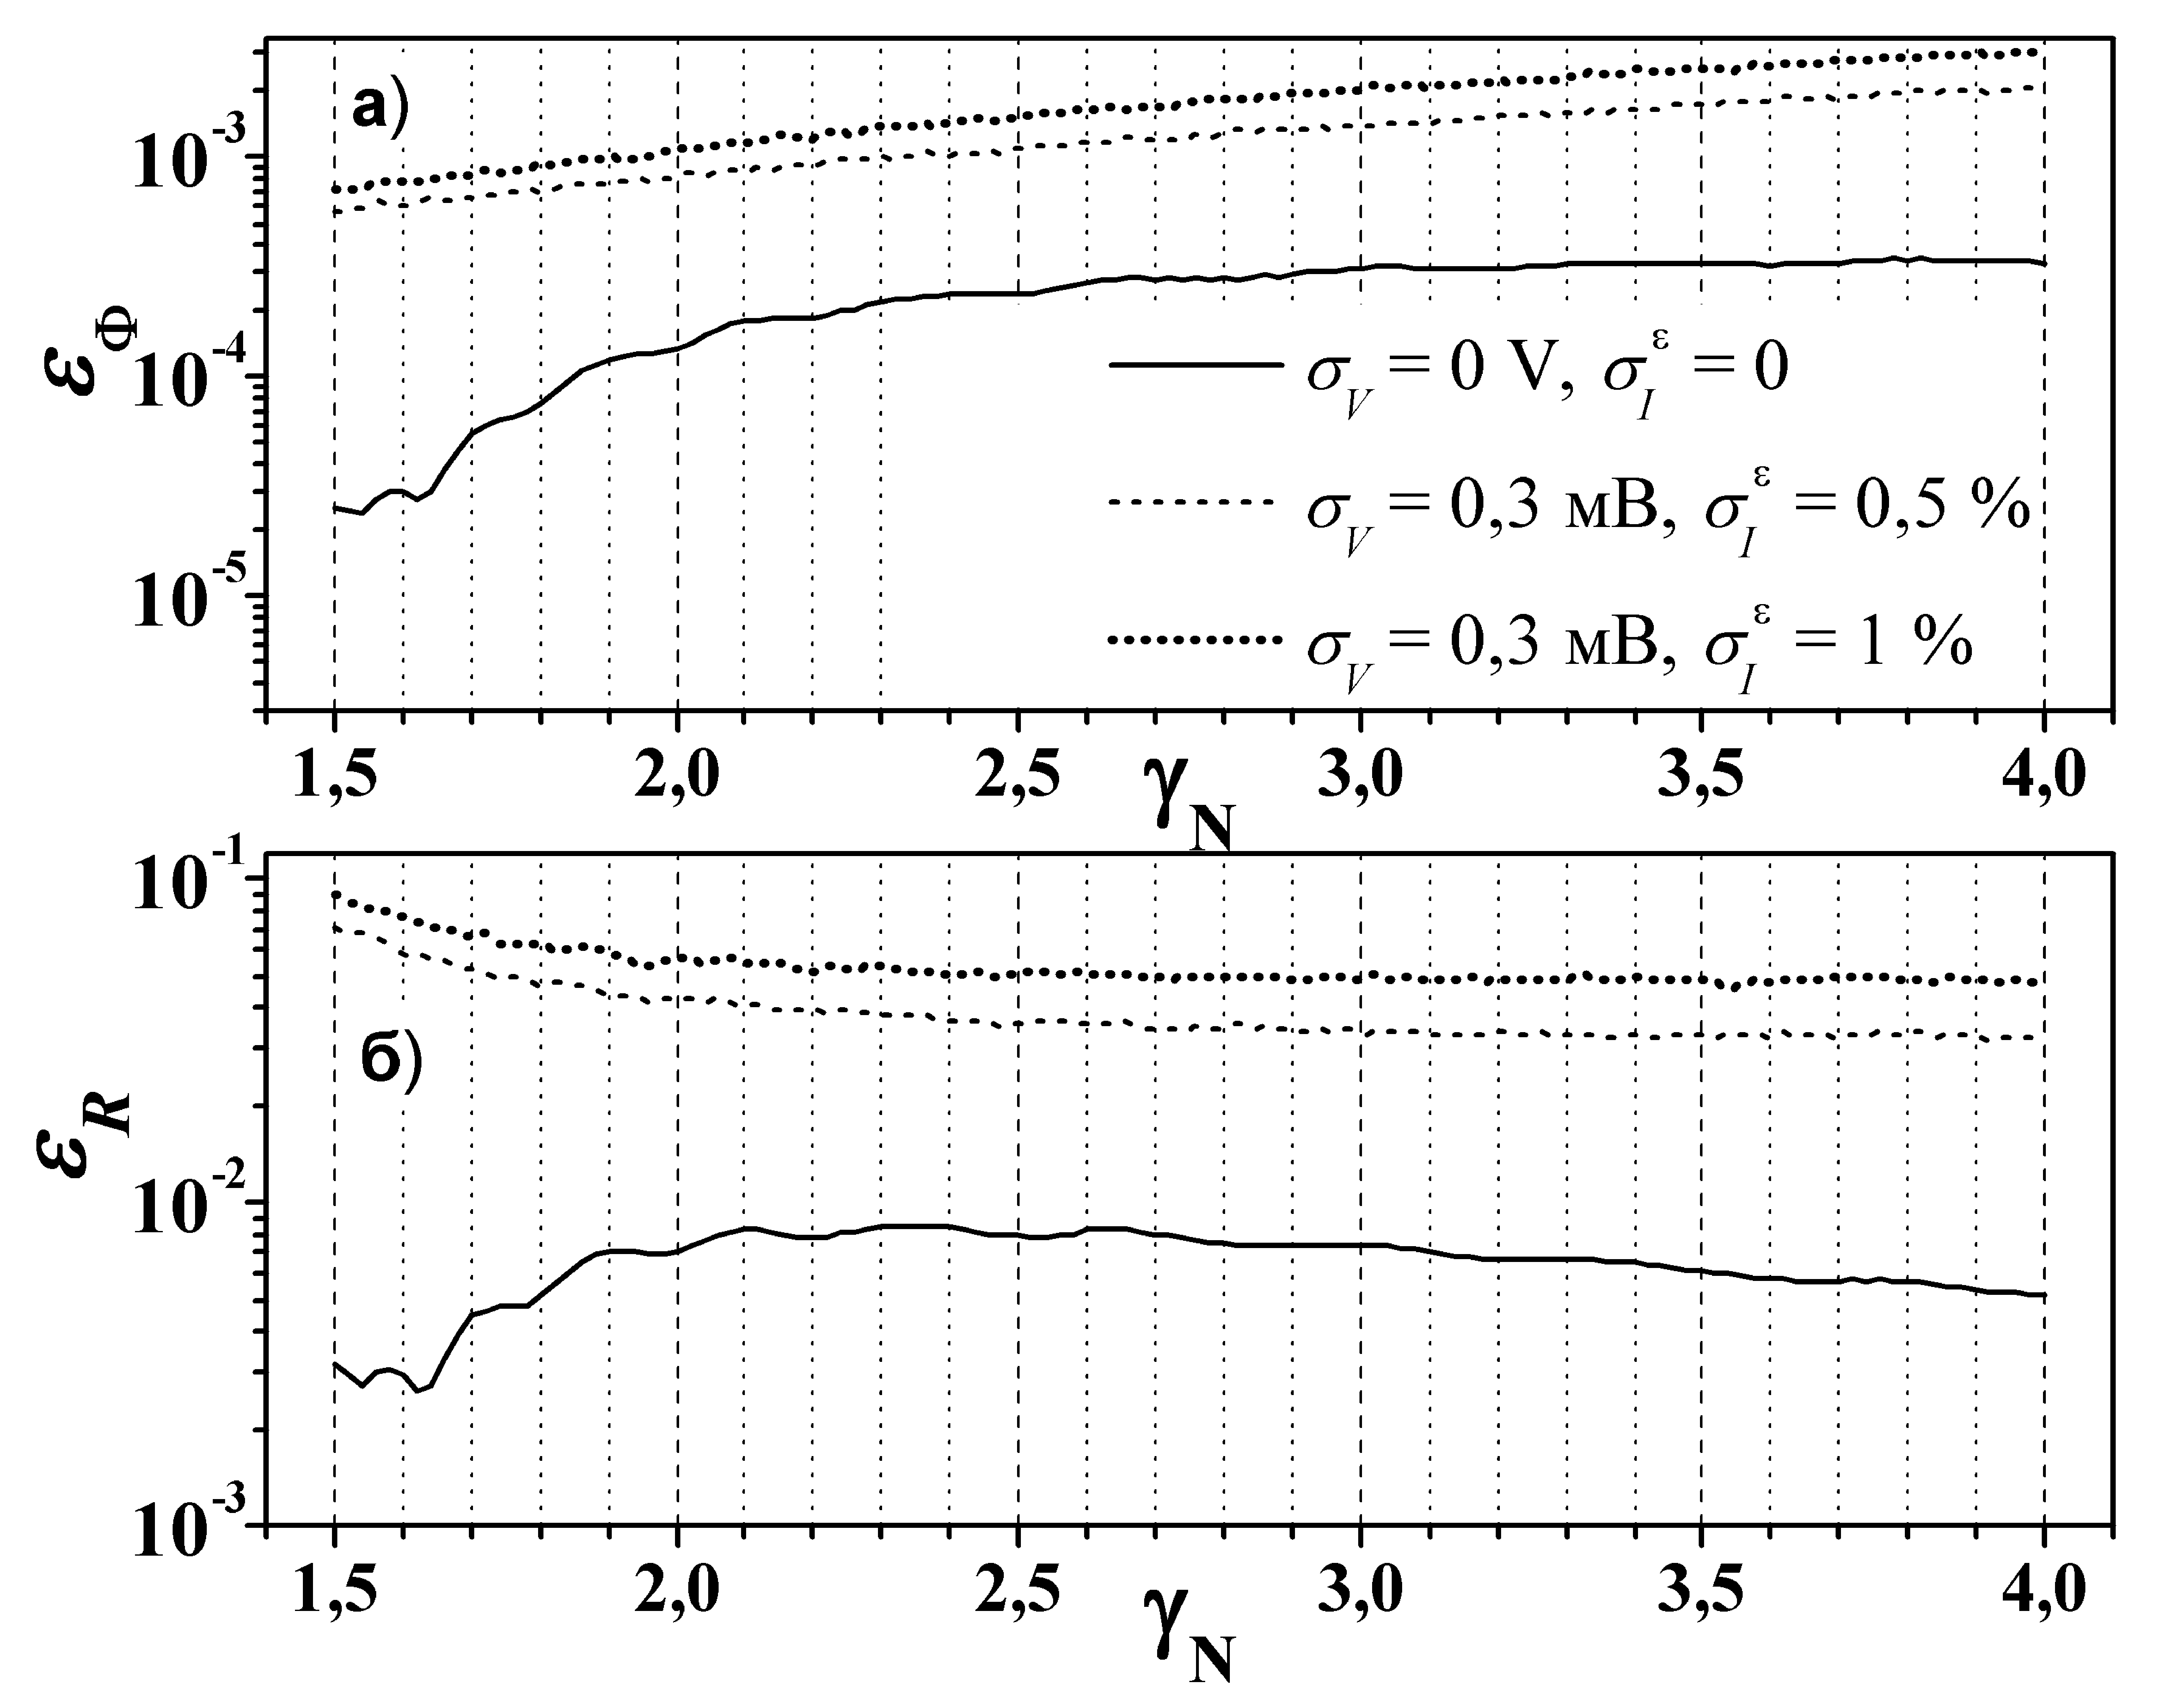
\includegraphics[width=0.6\textwidth]{figNorde}%
\caption{\label{figNorde}
Залежності похибки визначення $\Phi_b$ (a) та $R_s$ (б)  від величини $\gamma_N$.
 при застосуванні метода Норда до набору ідеальних синтезованих ВАХ (суцільні лінії) та зашумлених даних (штрихові лінії)
}
\end{figure}

J.~Werner  \cite{Werner} показав, що у випадку, коли падіння напруги в області бар'ру $V_d=(V-IR_s)\gg nkT/q$, то
\begin{equation}
\label{eqWerner}
\frac{(dI/dV)}{I}=\frac{q}{nkT}\left[1-R_s\left(\frac{dI}{dV}\right)\right].
\end{equation}
Рівняння~(\ref{eqWerner}) показує, що графік  залежності   $(dI/dV)/I$  від $(dI/dV)$ має бути прямою лінією,
причому її нахил та точка перетину з вертикальною віссю визначаються $R_s$ and $n_\mathrm{id}$.

На жаль, даний метод дозволяє визначити лише два параметри ДШ.
Для оцінки величини ВБШ була використана наступна процедура.
Спираючись на визначене значення $R_s$, експериментальна або синтезована ВАХ корелювалася і проводилась побудова залежності  $\ln I$ від $V_d$.
Після цього проводилась апроксимація отриманої залежності лінійною функцією за методом найменших квадратів \cite[с.~67]{KalitkinBook} в діапазоні $V_d>3kT/q$.
Необхідно підкреслити, що під час апроксимації нахил кривої може розглядатися або як незалежна величина, яка обчислюється, або як відома величина, що визначається попередньо визначеним (під час апроксимації функції (\ref{eqWerner})) значенням $n_\mathrm{id}$.
У роботі розглянуто обидва випадки.
Якщо величини $R_s$ and $n_\mathrm{id}$ визначались шляхом лінійної апроксимації функції (\ref{eqWerner}), а $\Phi_b$ --- як перетин залежності $\ln I=f(V_d)$ при відомому нахилі, то використовується позначення <<Werner>>.
Якщо ж лише $R_s$ визначається за допомогою функції Вернера (\ref{eqWerner}), а $\Phi_b$ and $n_\mathrm{id}$ обчислюються потім із залежності $\ln I=f(V_d)$, то використовується позначення <<Werner*>>.
Подібний підхід до позначень отриманих результатів (із зірочкою та без неї залежно від того, скільки незалежних величин використовується при апроксимації ВАХ, скорельованих відповідно до визначеного раніше значення послідовного опору) використовуються і для інших методів, детальніше описаних нижче.

R.~Cibils  та R.~Buitrago \cite{Cibils} запропонували використовувати допоміжну функцію у вигляді
\begin{equation}
\label{eqCibils}
F_a(V)=V-V_a\ln I,
\end{equation}
де
$V_a$ практично довільне значення напруги, $V_a\geq99,5I_sR_s+n_\mathrm{id}kT/q$.
Якщо $I_{min,a}$ --- це значення струму, яке відповідає напрузі $V_{min}$, при якій спостерігається мінімум функції $F_a(V)$,
то залежність $I_{min,a}$ від $V_a$ має бути \cite{Cibils} лінійною:
\begin{equation}
\label{eqCibilsDet}
I_{min,a}=(V_a-n_\mathrm{id}kT/q)/R_s\,.
\end{equation}
У роботі при побудові сімейства допоміжних функцій згідно з виразом (\ref{eqCibils}) використовувалися значення  $V_a$ в діапазоні від 0,035~В до максимального значення напруги для даної ВАХ.
Крок зміни $V_a$ дорівнював 1~мВ.
Отримані результати позначені міткою <<Cibils>>.

А.~Kaminski зі співавторами \cite{Kaminski} запропонували два методи.
Перший використовує допоміжну функцію, яка будується з використанням інтегрування ВАХ.
Ордината та абсциса $j-$ої точки допоміжного графіку розраховуюся як
\begin{equation}
\label{eqKam1}
Y_j=\frac{1}{I_j-I_1}\int_{V_1}^{V_j}I\,dV \quad\text{and}\quad X_j=\frac{I_j+I_1}{2},
\end{equation}
де
$V_i$ та $I_i$ --- це координати $i-$ої точки ВАХ,
$i\in(1,\ldots, N_p)$,
$j\in(2,\ldots, N_p)$,
$N_p$ --- загальна кількість точок ВАХ.
Згідно з цим методом очікується, що залежність $Y$ від $X$ має бути лінійною:
\begin{equation}
\label{eqKam1Det}
Y=n_\mathrm{id}kT/q+R_sX.
\end{equation}
Тобто лінійна апроксимація допоміжної функції дозволяє визначити $R_s$ та $n_\mathrm{id}$.

У роботі лінійна апроксимація здійснювалась за допомогою методу найменших квадратів.
Числове інтегрування ВАХ здійснювалось за методом трапецій \cite[с.~98]{KalitkinBook}.
Отримані результаті позначені мітками <<Kaminski I>> та <<Kaminski* I>>.

У другому методі, розглянутому в роботі \cite{Kaminski}, також використовується допоміжна функція $Y$ від $X$, проте
\begin{equation}
\label{eqKam2}
Y_k=\frac{\ln(I_j/I_i)}{I_j-I_i} \quad\text{and}\quad X_k=\frac{V_j-V_i}{I_j-I_i},
\end{equation}
$i\in(1,\ldots, N_p-1)$,
$j\in(i+1,\ldots, N_p)$,
$k\in(1,\ldots, N_p(N_p-1)/2)$.
Отримана таким чином залежність має бути прямолінійною:
\begin{equation}
\label{eqKam2Det}
Y=q(-R_s+X)/n_\mathrm{id}kT.
\end{equation}
Отримані за допомогою даного підходу результати позначені мітками <<Kaminski II>> та <<Kaminski* II>>.

У методі, запропонованому в роботі \cite{Bohlin}, використовуються дві функції Норда, побудовані з використанням двох різних значень $\gamma_N$:
\begin{eqnarray}
\label{eqBohlin}
F_1(V)&=&V/\gamma_1-kT/q\cdot\ln(I/AA^*T^2),
\nonumber\\
F_2(V)&=&V/\gamma_2-kT/q\cdot\ln(I/AA^*T^2).
\end{eqnarray}
Передбачено, що параметри ДШ визначаються за допомогою співвідношень
\begin{eqnarray}
\label{eqBohlinDet}
n_\mathrm{id}&=&\frac{1}{2}\left[\frac{\gamma_1I_{min,2}-\gamma_2I_{min,1}}{I_{min,2}-I_{min,1}}+\right.
\\
&&\left.\frac{V_{min,1}-V_{min,2}+(\gamma_2-\gamma_1)kT/q}{F_2(V_{min,2})-F_1(V_{min,1})-V_{min,2}/\gamma_2+V_{min,1}/\gamma_1}\right]
,\nonumber
\\
Rs&=&\frac{kT}{2q}\left[\frac{\gamma_1-n_\mathrm{id}}{I_{min,1}}+\frac{\gamma_2-n_\mathrm{id}}{I_{min,2}}\right]\,,
\\
\Phi_b&=&\frac{1}{2}\left[F_1(V_{min,1})+\frac{(\gamma_1-n_\mathrm{id})(qV_{min,1}-\gamma_1kT)}{\gamma_1qn_\mathrm{id}}\,+\right.
\nonumber\\
&&\left.F_2(V_{min,2})+\frac{(\gamma_2-n_\mathrm{id})(qV_{min,2}-\gamma_2kT)}{\gamma_2qn_\mathrm{id}}\right].
\end{eqnarray}
де
$[F_1(V_{min,1}), V_{min,1}]$ та $[F_2(V_{min,2}), V_{min,2}]$ --- це координати мінімумів функцій  $F_1(V)$ від $V$ та $F_2(V)$ від $V$, відповідно;
$I_{min,1}$ та $I_{min,2}$ --- значення струму, які відповідають на ВАХ значенням напруги $V_{min,1}$ та $V_{min,2}$, відповідно.

Проведені числові дослідження показали, що, як і в методі Норда, у цьому випадку точність визначення параметрів залежить від вибору величин $\gamma_1$ та $\gamma_2$.
Отримані результати приведені на рис.~\ref{figBohlin}.
Виявлено, що похибка екстрагування параметрів зростає при збільшенні модуля різниці параметрів $|\gamma_1-\gamma_2|$.
Мінімальні похибки спостерігаються при використанні величин $\gamma_1=1,6$ та $\gamma_2=3,5$, які і використовувалися під час порівняльного аналізу.
Отримані результати позначені міткою <<Bohlin>>.

\begin{figure}
\center
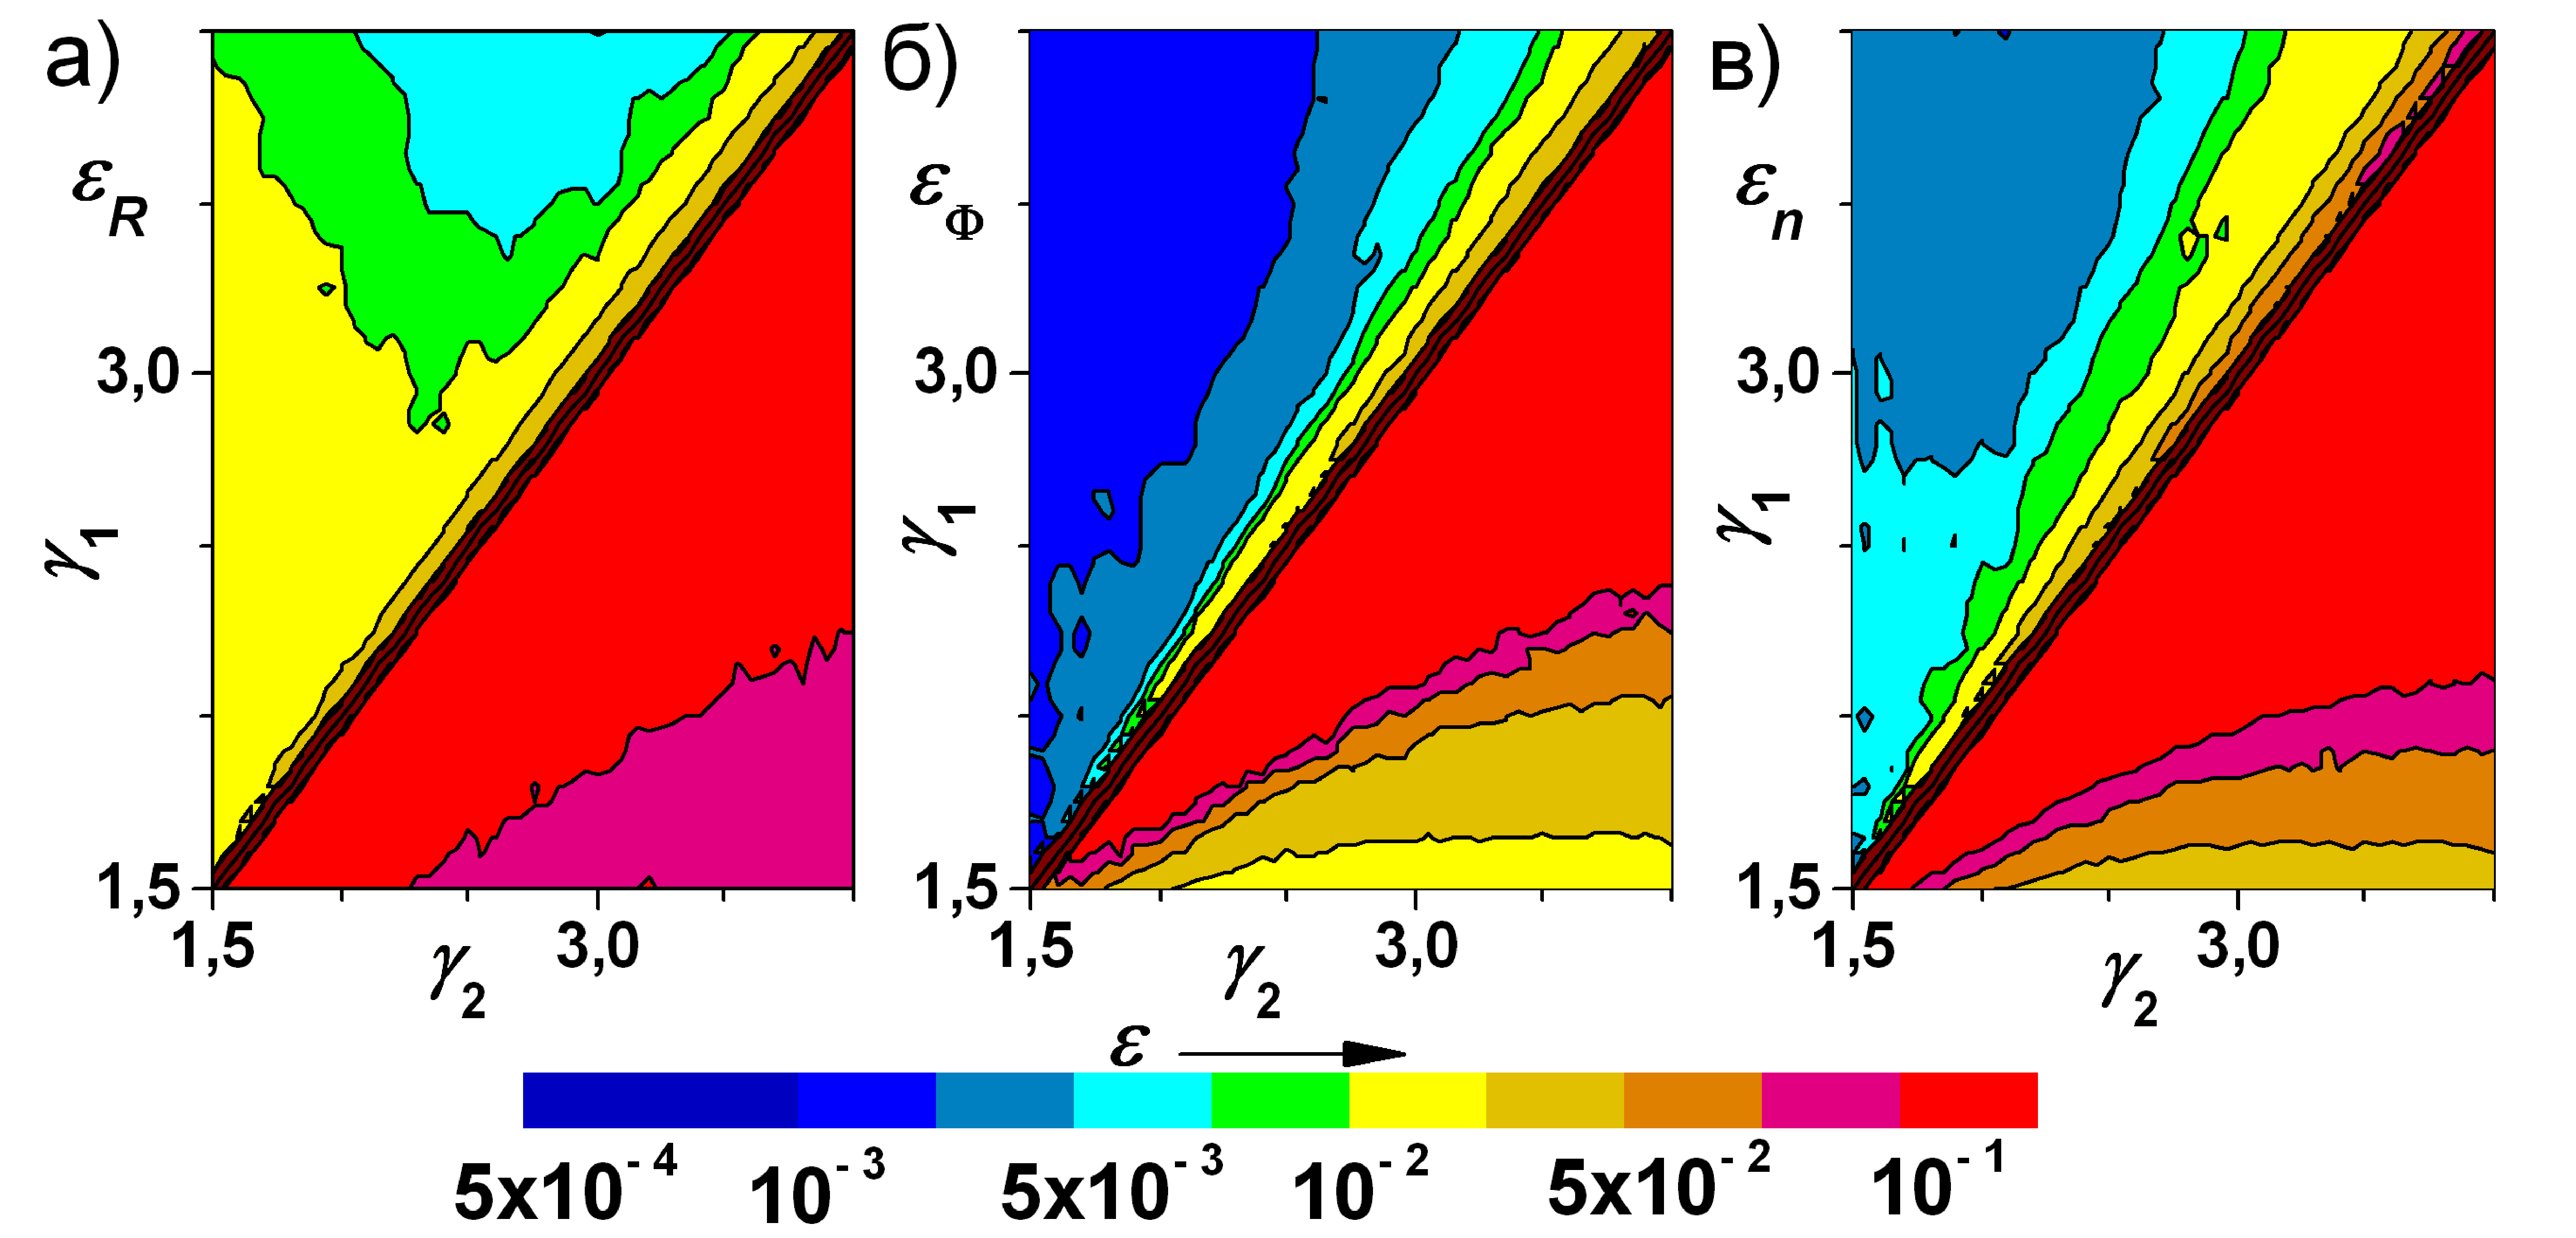
\includegraphics[width=0.8\textwidth]{figBohlin}%
\caption{\label{figBohlin}
Залежності похибок визначення $R_s$ (a), $\Phi_b$ (б) та $n_\mathrm{id}$ (в) від величини параметрів $\gamma_1$ та $\gamma_2$ при застосуванні метода Бохліна.
Наведено результати, отримані для наборів ідеальних ($\sigma_V=0$~V, $\sigma_I^\varepsilon=0$) синтезованих ВАХ (область $\gamma_1>\gamma_2$) та зашумлених ($\sigma_V=0,3$~мВ, $\sigma_I^\varepsilon=1\%$) даних (область $\gamma_2>\gamma_1$)
}
\end{figure}

У роботі \cite{Lee} запропоновано використовувати масив функцій $\{F_L(I)\}$:
\begin{equation}
\label{eqLee}
F_L(I)=V(I)-V_a\ln I,
\end{equation}
де
$V_a$ --- це довільне значення напруги.
Кожна з функцій $F_L(I)$ має бути апроксимована залежністю
\begin{equation}
\label{eqGrFit}
y(I)=c_1+c_2I+c_3\ln I
\end{equation}
а параметри $c_1$, $c_2$ та $c_3$ --- визначені.
Тоді очікується \cite{Lee}, що при $V>3kT/q$,
залежність $I_a=-c_3/c_2$ від $V_a$ має бути лінійною:
\begin{equation}
\label{eqLeeDet}
I_a(V_a)=(-n_\mathrm{id}kT/q+V_a)/R_s,
\end{equation}
що дозволяє визначити послідовний опір та фактор неідеальності.
У свою чергу, $\Phi_b$ може бути розрахований \cite{Lee} за допомогою виразу
\begin{equation}
\label{eqLeeFb}
\Phi_b=c_3/n_\mathrm{id}+kT/q\cdot\ln\left(AA^*T^2\right).
\end{equation}

У роботі при застосуванні цього методу використовувалися значення $V_a$ починаючи з 40~мВ із кроком 20~мВ;
апроксимація $F_L(I)$ здійснювалась із використанням методу найменших квадратів.
Отримані дані позначені міткою <<Lee>>.

У роботі Д.~Громова та В.~Пугачевича \cite{Gromov} розглянуто два можливі шляхи визначення параметрів ДШ.
Згідно з першим із них залежність, напруги від струму має бути апроксимована виразом (\ref{eqGrFit}) причому
\begin{eqnarray}
\label{eqGr1}
R_s&=&c_2\,,
\\
n_\mathrm{id}&=&(c_3q)/(kT)\,,
\\
\Phi_b&=&\left[c_1/c_3+\ln\left(AA^*T^2\right)\right]kT/q\,.
\end{eqnarray}
Другий шлях полягає у тому, що вираз (\ref{eqGrFit}) застосовується до апроксимації функції Норда з $\gamma_N=2$:
\begin{equation}
\label{eqGr2}
F(I)=V(I)/2-kT/q\cdot\ln(I/AA^*T^2).
\end{equation}
При цьому \cite{Gromov}
\begin{eqnarray}
\label{eqGr2Det}
R_s&=&2c_2\,,
\\
n_\mathrm{id}&=&(2c_3q)/(kT)+2\,,
\\
\Phi_b&=&\frac{2c_1}{n_\mathrm{id}}+\frac{(2-n_\mathrm{id})kT}{n_\mathrm{id}q}\ln\left(AA^*T^2\right)\,.
\end{eqnarray}
Застосування методів показало, що обидва підходи приводять до абсолютно однакових результатів.
Більше того, визначені значення параметрів дуже близькі до даних, які отримані за однакових початкових умов при використанні методу, описаного в роботі \cite{Lee} та згаданого раніше.
Тобто ці методи не є незалежними.

З іншого боку, проведені оцінки показали, що точність визначення параметрів за допомогою цих методів залежить від діапазону вихідної ВАХ, який використовується для побудови допоміжної функції, яка потім апроксимується залежністю (\ref{eqGrFit}).
На рис.~\ref{figGromov} наведено залежності похибок екстрагованих параметрів від початкового значення діапазону напруг, в якому проводилась апроксимація.
Видно, що для ідеальних ВАХ точність підвищується при звуженні використаного діапазону.
Водночас для зашумлених даних залежність немонотонна і екстремальне значення точності спостерігається при певних значеннях ширини діапазону.
Причому ширина та положення діапазону, при якому точність визначення параметрів найвища, залежить від рівня шуму.



\begin{figure}
\center
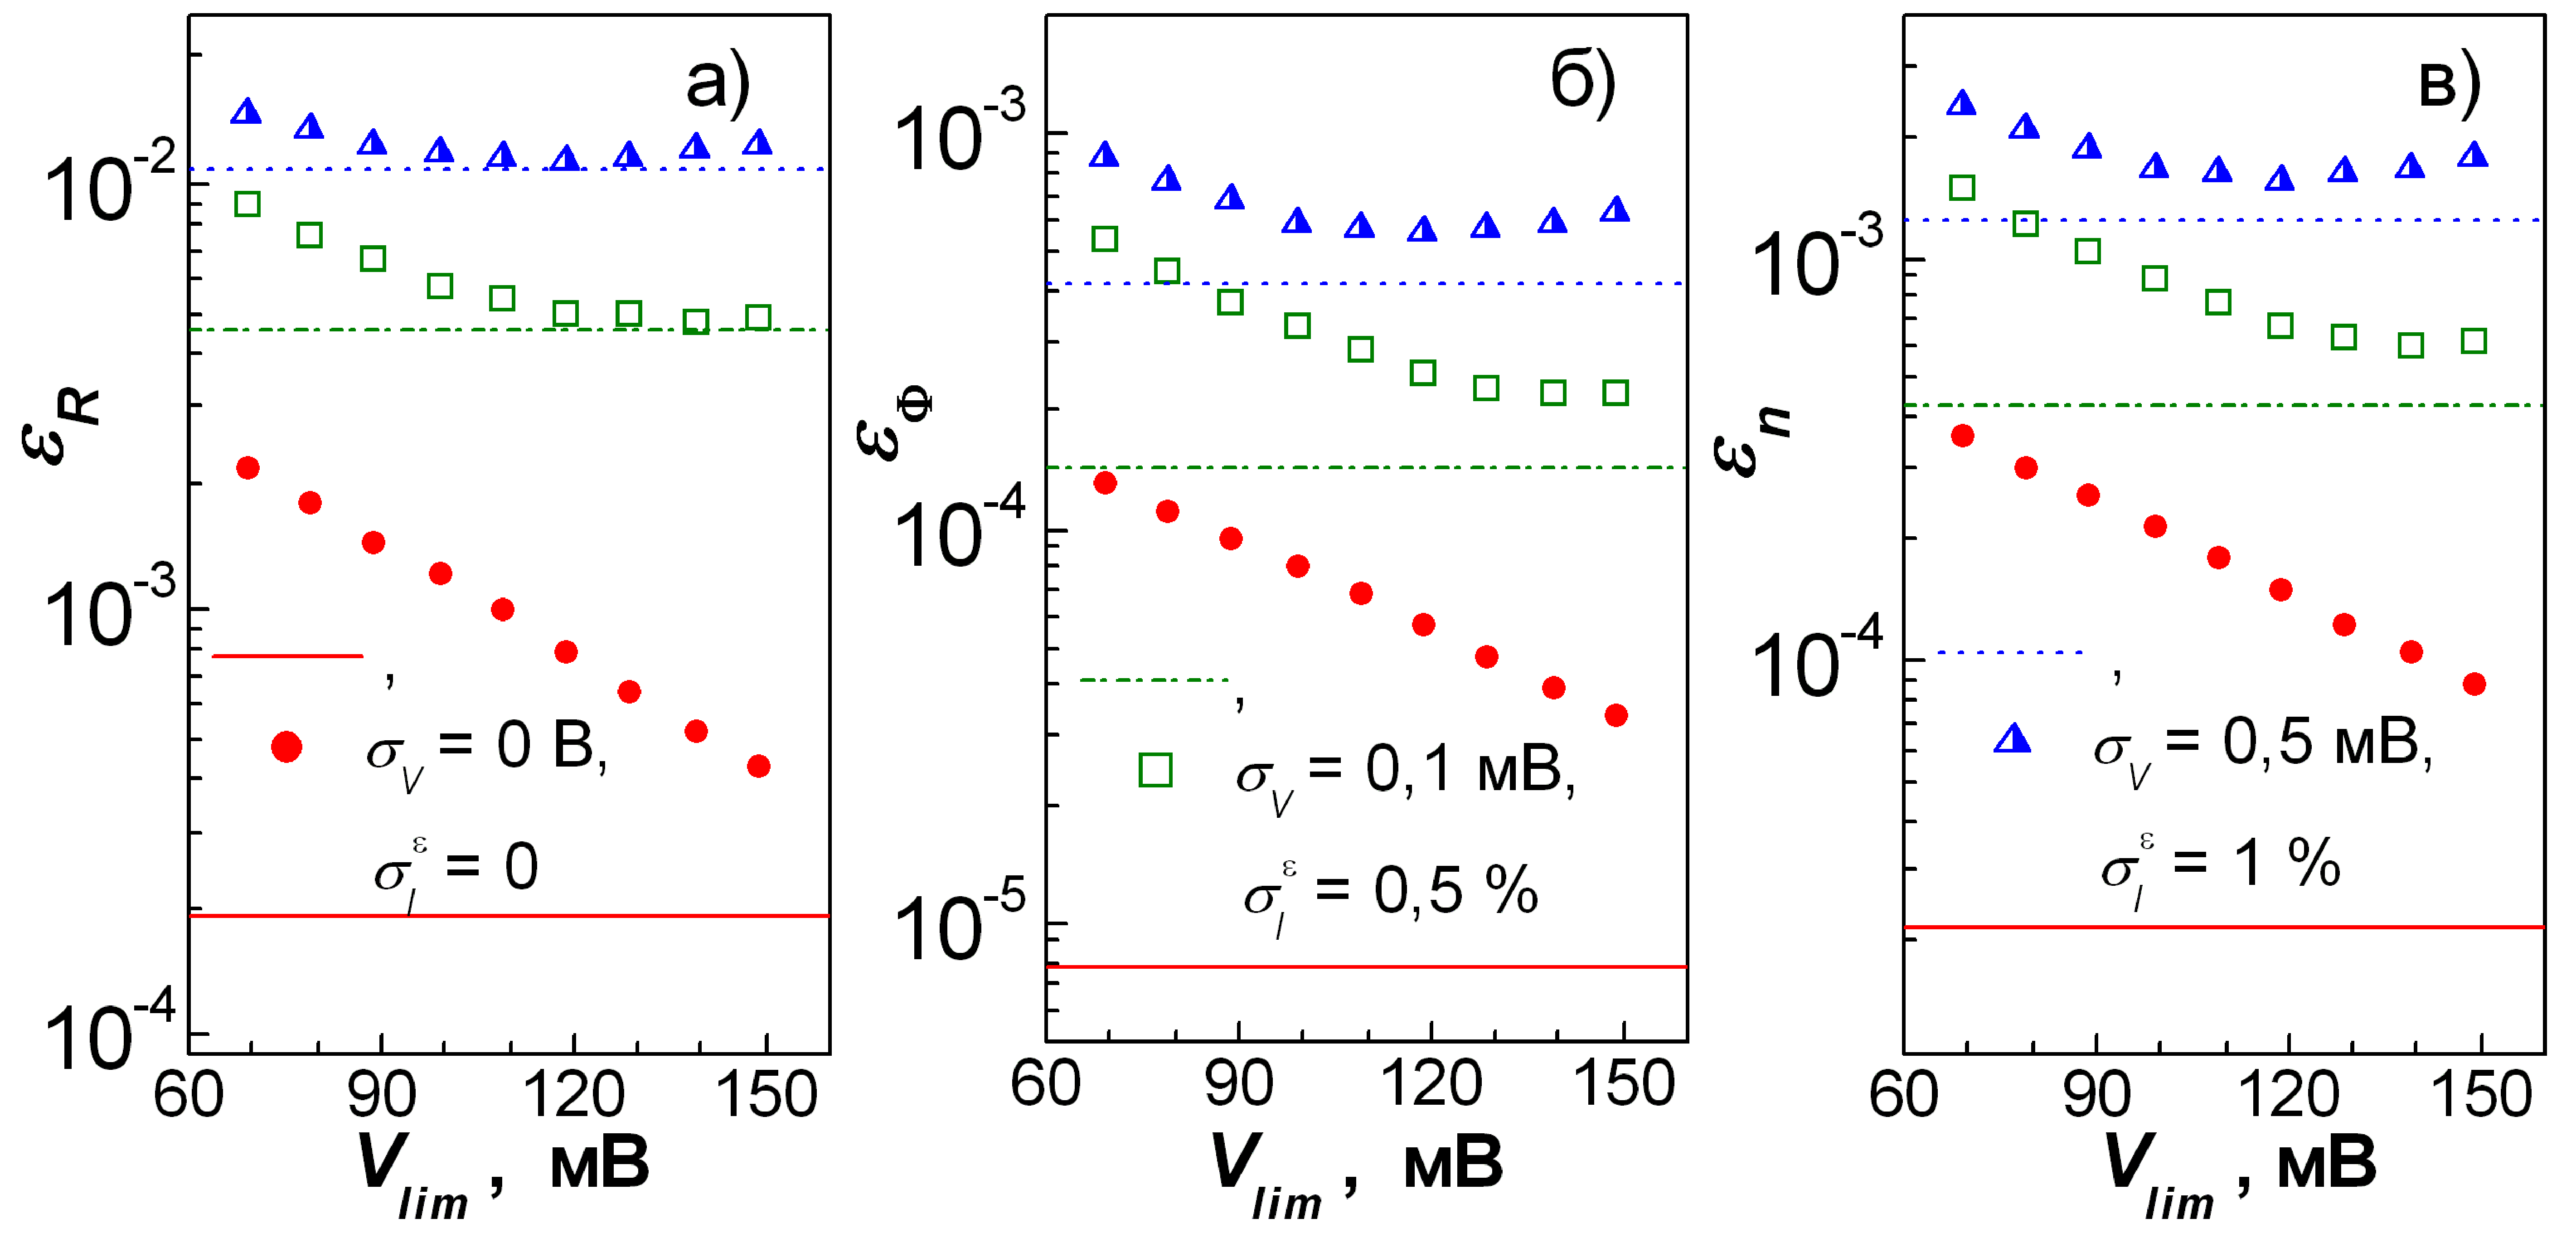
\includegraphics[width=0.9\textwidth]{figGromov}%
\caption{\label{figGromov}
Залежності похибок визначення $R_s$ (a), $\Phi_b$ (б) та $n_\mathrm{id}$ (в) при використанні методу Громова.
Наведено результати, отримані при апроксимуванні залежністю (\ref{eqGrFit}) допоміжної функції, побудованої
на основі ділянки ВАХ в діапазоні напруг від $V_{lim}$ до максимально значення.
Горизонтальні лінії вказують похибки значень параметрів ДШ, які отримані при використанні адаптивної процедури (див. текст).
Результати отримані при застосуванні методу до ідеальних синтезованих ВАХ (заповнені кружечки, суцільні лінії) та зашумлених даних
з $\sigma_V=0,1$~мВ та $\sigma_I^\varepsilon=0,5\%$ (незаповлені квадрати, штрих--пунктирні лінії) та з $\sigma_V=0,5$~мВ та $\sigma_I^\varepsilon=1\%$
(напівзаповнені трикутники, пунктирні лінії)
}
\end{figure}

У зв'язку з цим, для покращення ефективності роботи методів Громова та Лі, пропонується використовувати спеціальну адаптивну процедуру вибору діапазону побудови допоміжної функції.
Вона полягає у тому, що параметри визначаються для всіх можливих діапазонів, кількість яких залежить від кількості точок вихідної ВАХ.
Після цього для кожного отриманого набору параметрів обчислюється величина $\theta=\sum_{i=1}^{N_p}[1-I_{calc}(V_i)/I_i]^2$,
де $I_{calc}(V_i)$ розраховується з використанням виразів (\ref{eqSDIV}) та (\ref{eqSDIs}).
Найкращим за точністю вважається той набір параметрів, для якого спостерігається мінімум величини $\theta$.

Зрозуміло, що подібна адаптивна процедура збільшує час, необхідних для визначення параметрів ДШ через необхідність багатократного повторення застосування методу Громова (Лі) та додаткових розрахунків.
Проте, з іншого боку, ця процедура може бути автоматизована, а також дозволяє підвищити точність (лінії на рис.~\ref{figGromov}).

Нижче розглянуті результати застосування методу Громова із використанням запропонованої адаптивної процедури.
Отримані дані позначені міткою <<Gromov>>.
Різниця між ними та позначеними міткою <<Lee>> визначає, фактично, доцільність запропонованої процедури.

У роботі \cite{Cheung} запропоновано визначати параметри ДШ шляхом побудови залежностей функцій $H(V)$
\begin{equation}
\label{eqH}
H(I)=V-\frac{n_\mathrm{id}kT}{q}\ln\left(\frac{I}{AA^*T^2}\right).
\end{equation}
та $dV/d(\ln I)$ від сили струму.
За умови $V_d>3kT/q$ ці залежності мають бути лінійними, причому
\begin{eqnarray}
\label{eqChung}
\frac{dV}{d\ln I}&=&R_sI+n_\mathrm{id}kT/q,
\\
\label{eqHDet}
H(I)&=&n_\mathrm{id}\Phi_b+IR_s.
\end{eqnarray}
При застосуванні методу спочатку визначаються $R_s$ та  $n_\mathrm{id}$ на основі рівняння (\ref{eqChung}),
а потім  $\Phi_b$, використовуючи вираз~(\ref{eqHDet}) та обчислене на попередньому кроці значення $n_\mathrm{id}$.
Отримані результати позначені міткою <<Chung>>.

Ще одним методом, де використовуються диференційні коефіцієнти ВАХ, є запропонований в роботі \cite{Mikhelashvili}.
У цьому випадку все починається з обчислення функції  $\alpha(V)$:
\begin{equation}
\label{eqMikh}
\alpha(V)=d(\ln I)/d(\ln V).
\end{equation}
Визначення параметрів відбувається із використанням співвідношень
\begin{eqnarray}
\label{eqMikhDet}
R_s&=&\frac{V_{max}}{\alpha^2_{max}I_{max}}\,,
\\
n_\mathrm{id}&=&\frac{qV_{max}(\alpha_{max}-1)}{\alpha_{max}^2kT}\,,
\\
\Phi_b&=&\frac{kT}{q}\left[\alpha_{max}+1-\ln\left(\frac{I_{max}}{AA^*T^2}\right)\right]\,.\label{eqMikhDetFi}
\end{eqnarray}
де
$\alpha_{max}$ та $V_{max}$  це координати максимуму залежності $\alpha$ від $V$;
$I_{max}$ --- сила струму, яка відповідає напрузі $V_{max}$.

\begin{figure}
\center
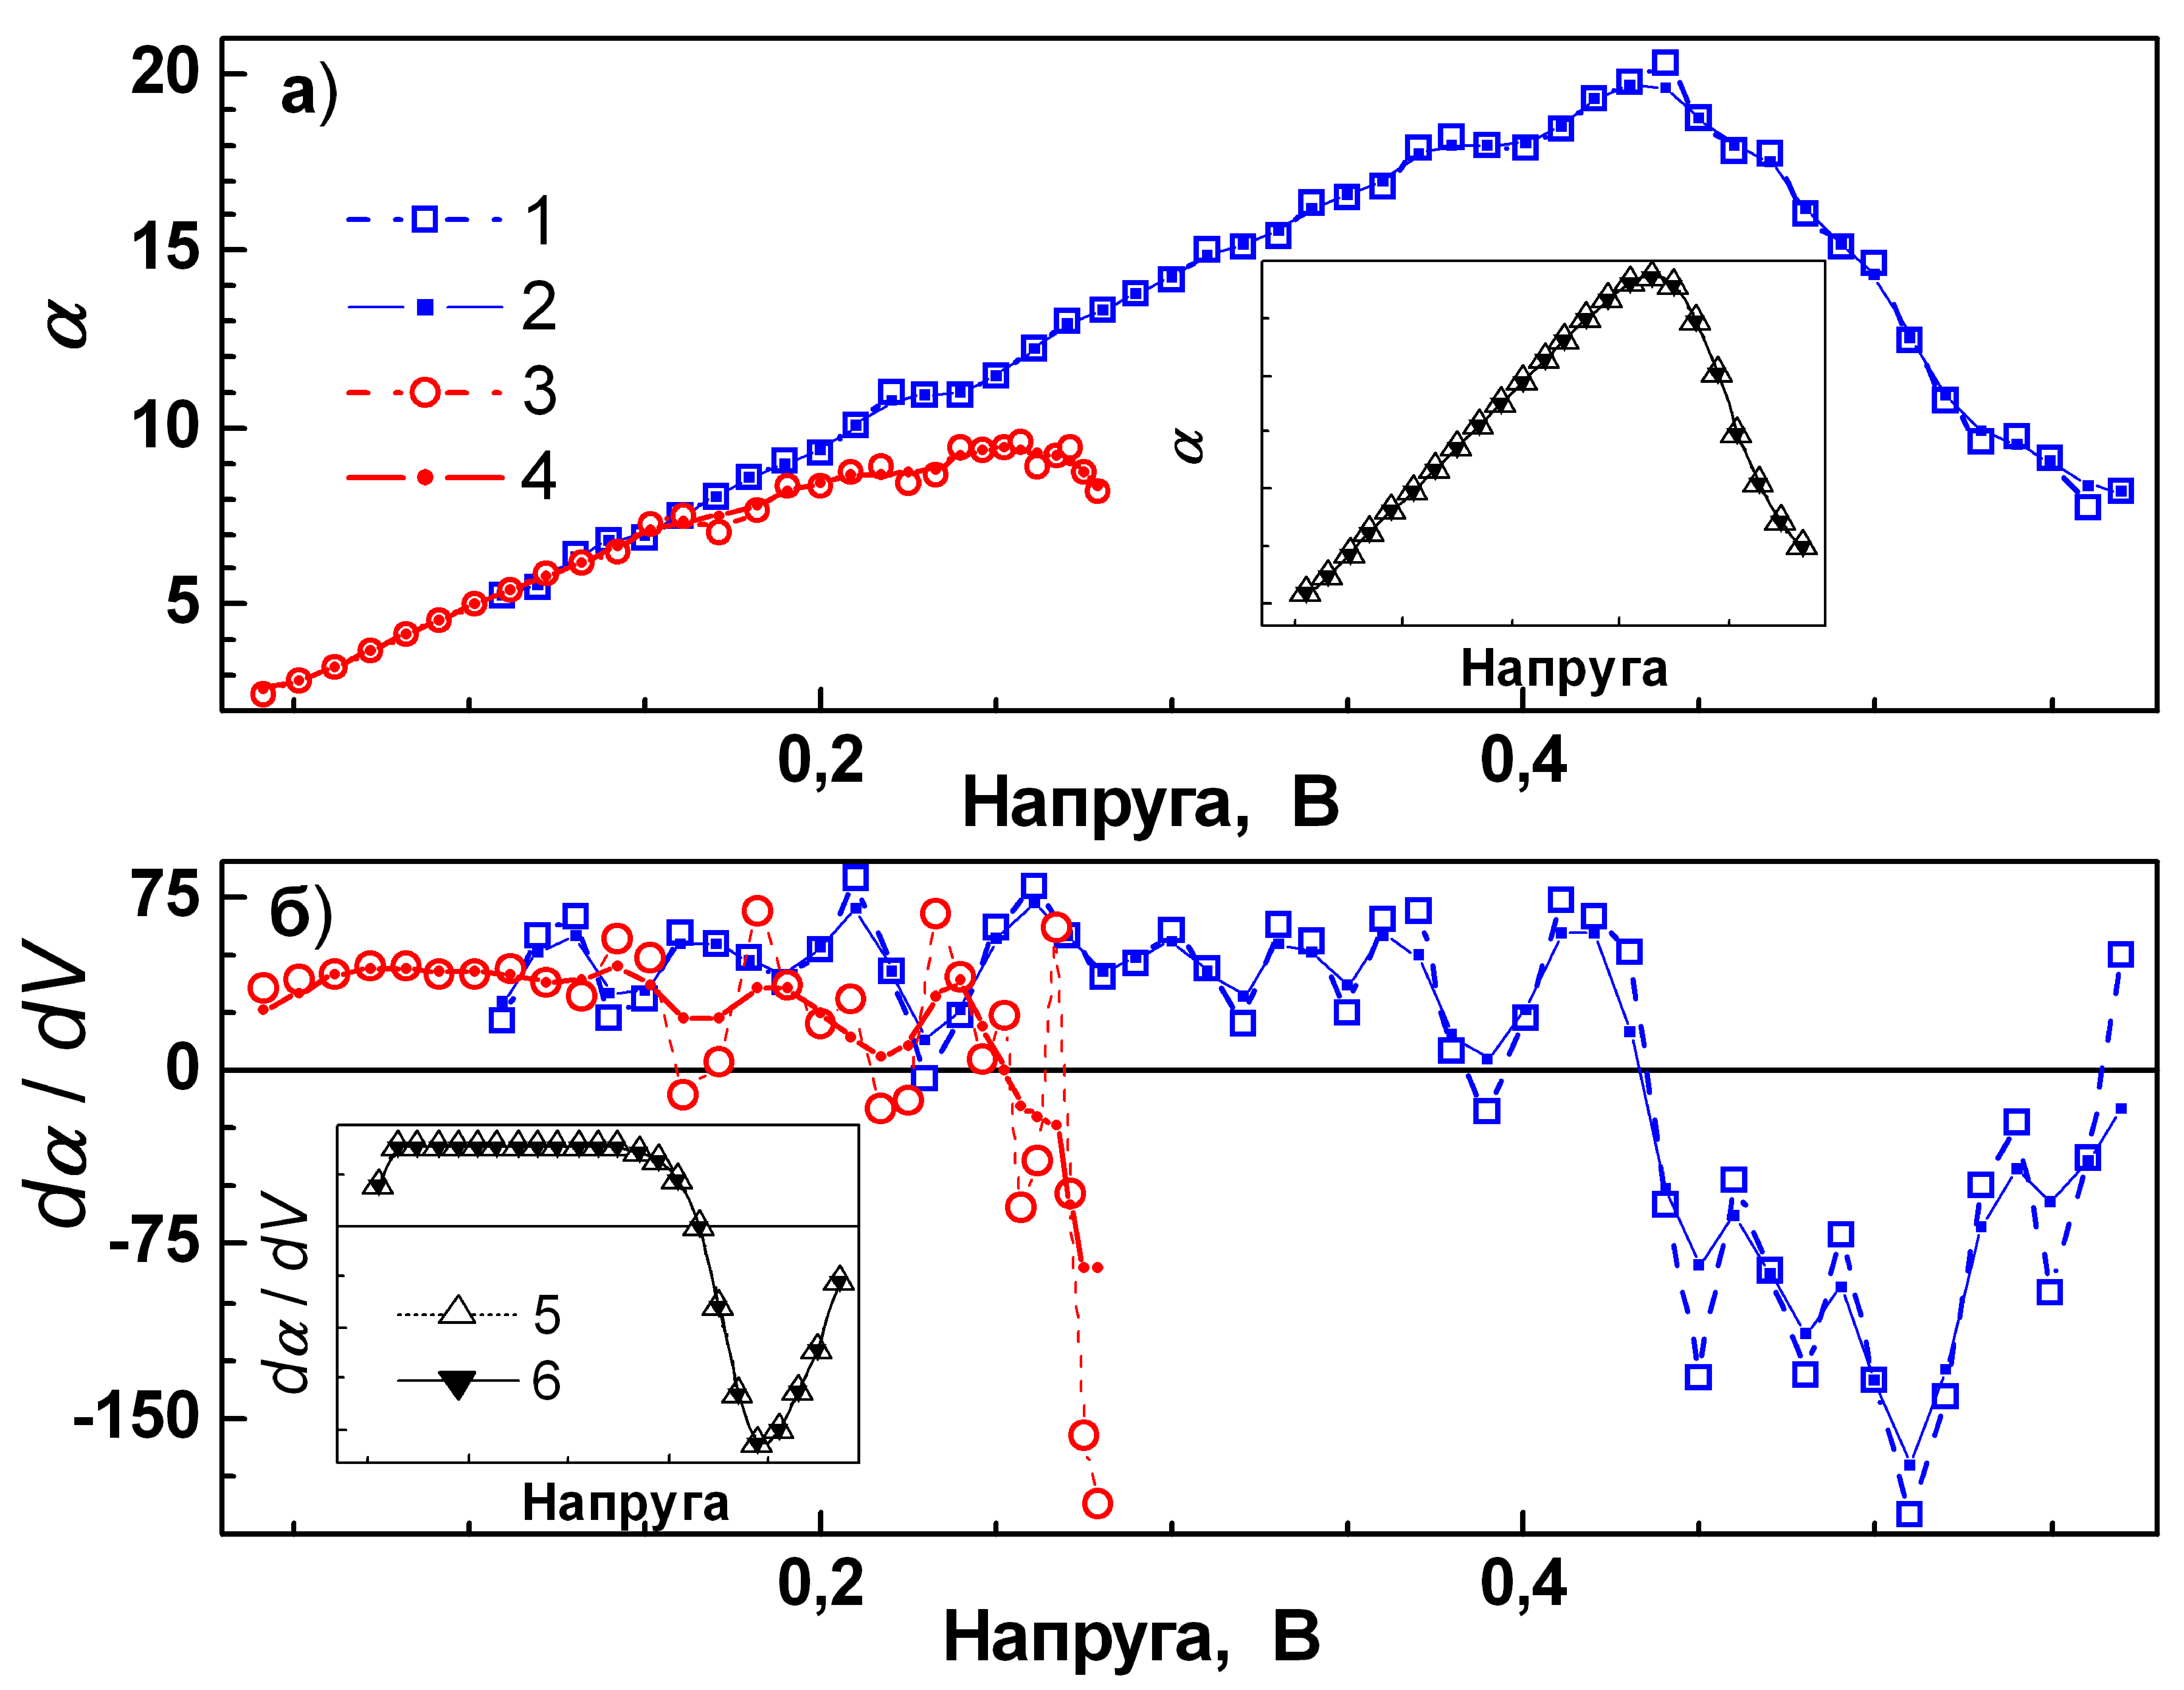
\includegraphics[width=0.65\textwidth]{figMikh}%
\caption{\label{figMikh}
Залежності функції~(\ref{eqMikh}) (а) та її похідної (б) від напруги.
Наведено графіки для зашумлених даних ($\sigma_V=0,3$~мВ, $\sigma_I^\varepsilon=1\%$, криві 1 та 2), для експериментально виміряних ВАХ (криві 3 та 4) та для ідеальних синтезованих ВАХ (вставка, криві 5 та 6) до (1, 3, 5) та після (2, 4, 6) запропонованої обробки
}
\end{figure}

Зауважимо, що однією з необхідних властивостей методу, які використовуються для обчислення параметрів пристроїв із набору ВАХ, отриманих за різних умов, є можливість його застосування в автоматичному режимі.
При цьому найпоширеніший варіантів пошуку екстремуму полягає у знаходженні нулів похідної.
Як видно з виразів (\ref{eqMikh})--(\ref{eqMikhDetFi}), для даного методу це означає необхідність проведення процедури числового визначення другої похідної ВАХ.


Рис.~\ref{figMikh}(a) показує, що при використанні експериментальних ВАХ чи зашумлених даних числове диференціювання викликає появу багаточисленних локальних екстремумів на залежності функції $\alpha$ від $V$.
Ці екстремуми заважають автоматичному виявленню точки максимуму через наявність багатьох нульових точок на залежності $d\alpha/dV$ від $V$ (рис.~\ref{figMikh},б).
З метою подолання цих труднощів, у роботі запропоновано проводити спеціальну 2--стадійну процедуру обробки даних.
А саме, на першій стадії обробки до отриманої з ВАХ залежності $\alpha$ від $V$ пропонується застосовувати 3--точковий медіанний фільтр, після чого, на другій стадії, проводити згладжування.
І лише після цього, проводити визначення положення максимуму, визначення величин $\alpha_{max}$, $V_{max}$  та $I_{max}$ і розрахунок величин параметрів ДШ.
Дані на рис.~\ref{figMikh} показують, що запропонована процедура обробки дійсно зменшує вплив побічних максимумів та дозволяє підвищити точність методу.
Згладжування здійснюється завдяки усередненню по трьом сусіднім точкам із ваговими коефіцієнтами, які визначаються розподілом Гауса з дисперсією, рівною 0,6.

Надалі наведено результати, позначені міткою <<Mikhelashvili>> та отримані з використанням зазначеної процедури обробки.


\subsection{Числові методи}
Визначення параметрів проводилося і з використанням стандартного методу найменших квадратів зі статистичними ваговими коефіцієнтами \cite[с.~67]{KalitkinBook}.
У цьому випадку необхідно мінімізувати квадратичну форму
\begin{equation}
\label{eqLS}
S(I_s,n_\mathrm{id},R_s)=\sum_{i=1}^{N_p}I_i^{-1}\left[I_i-I_{calc}(V_i,I_s,n_\mathrm{id},R_s)\right]^2,
\end{equation}
де $I_{calc}$ --- значення сили струму, отримане при інтерполяції.
При мінімізації шукався розв'язок системи рівнянь, отриманих із умов $\partial S/\partial I_s=0$,
$\partial S/\partial n_\mathrm{id}=0$ та $\partial S/\partial R_s=0$.
Пошук розв'язку цієї системи нелінійних рівнянь проводився за допомогою методу покоординаткого градієнтного спуску \cite[с.~231]{KalitkinBook}.
Як критерій зупинки ітераційного процесу вибрано умову $\mid(S_j-S_{j+1})/S_j\mid<10^{-12}$,
де $S_j$ --- це значення квадратичної форми на $j-$му кроці ітерації.
Початкове наближення величини $R_s$ обчислювалося шляхом визначення перетину з координатною віссю залежності $(dV/dI)/I$ від $1/I$,
побудованої з використанням останніх п'яти точок ВАХ.
Початкові наближення $I_s$ та $n_\mathrm{id}$ отримувалися шляхом лінійної апроксимації залежності $\ln I$ від $V_d$, причому для визначення останньої величини використовувалися початкове наближення  $R_s$.

Розглянуто два варіанти методу найменших квадратів.
У першому з них для обчислення $I_{calc}$ використовувався вираз ~(\ref{eqSDIV}), тобто квадратична форма мала вигляд
\begin{equation}
\label{eqLSOrd}
S(I_s,n_\mathrm{id},R_s)=\sum_{i=1}^{N_p}I_i^{-1}\left[I_i-I_s\left\{\exp\left[\frac{q(V_i-I_iR_s)}{n_\mathrm{id}kT}\right]-1\right\}\right]^2.
\end{equation}
Отримані внаслідок мінімізації функції~(\ref{eqLSOrd}) результати позначені міткою <<Ordinary LS>>.

У другому випадку при побудові квадратичної форми використовувалася $W$--функція Ламберта.
За визначенням, функція $W$ є розв'язком рівняння $z=W(z)\cdot\exp(W(z))$, її значення обчислюються за допомогою ряду \cite{LambertBook}.
Згідно з результатами, розглянутими в роботі \cite{Lambert_Jung}, явний розв'язок  трансцендентного рівняння~(\ref{eqSDIV}) може бути виражений за допомогою основної гілки функції Ламберта, причому при нехтуванні впливом опору шунтування він має вигляд
\begin{equation}
\label{eqLam}
    I(V)=\frac{n_\mathrm{id}kT}{qR_s}W\left\{\frac{qR_s}{n_\mathrm{id}kT}
      \exp\left[\frac{q(V+R_sI_s)}{n_\mathrm{id}kT}\right]  \right\}+I_s.
\end{equation}
Тобто квадратична форма може бути записана у вигляді
\begin{equation}
\label{eqLSLamb}
S(I_s,n_\mathrm{id},R_s)=\sum_{i=1}^{N_p}I_i^{-1}\left[I_i-\frac{n_\mathrm{id}kT}{qR_s}W\left\{\frac{qR_s}{n_\mathrm{id}kT}
      \exp\left[\frac{q(V_i+R_sI_s)}{n_\mathrm{id}kT}\right]  \right\}-I_s\right]^2,
\end{equation}
Результати, отримані при мінімізації (\ref{eqLSLamb}), позначені міткою <<Lambert LS>>.


\subsection{Еволюційні алгоритми\label{subEA}}
Еволюційні алгоритми -- це клас обчислювальних оптимізаційних моделей, які при своїй побудові та реалізації імітують поведінку живої природи.
Під час роботи вони оперують наборами (популяціями) $P$ можливих розв'зків
$\overrightarrow{X}$: $P=\left\{\overrightarrow{X_k}\right\}$, $k\in(1,\ldots, N_S)$,
де $N_S$ --- це загальна кількість розв'язків у популяції.
Кожний із проміжних розв'язків є вектором, що складається з дійсних чисел:
$\overrightarrow{X_k}=\left\{x_{k,i}\right\}$, $i\in(1,\ldots, N_D)$,
де
$N_D$ дорівнює загальній кількості параметрів, які слід оптимізувати.
У нашому випадку $N_D=3$, $\overrightarrow{X}=\left\{R_s\,,\,n_\mathrm{id}\,,\,\ln I_s\right\}$.

Перед початком оптимізаційного процесу створюється початкова популяція.
Зазвичай початкові значення параметрів вибираються випадковим чином з інтервалу
$[\overrightarrow{X}^{L}, \overrightarrow{X}^{H}]$:
\begin{equation}
\label{eqEAIn}
x_{k,i,0}=x_i^L+r_{[0,1]}(x_i^H-x_i^L),
\end{equation}
де
$r_{[0,1]}$ --- випадкове число, рівномірно розподілене на інтервалі $[0,1]$,
$\overrightarrow{X}^{L}=\left\{x_i^L\right\}$ та $\overrightarrow{X}^{H}=\left\{x_i^H\right\}$ ---
нижня та верхня межі простору, де шукаються розв'язки, відповідно.
У роботі проводився пошук у просторі, обмеженого наступним чином:
$R_s\in[0,\,50]$~Ом, $n_\mathrm{id}\in[1,\,2]$, $I_s\in[10^{-26},\,10^{-2}]$~A.

На кожному кроці ітерації
а)~проводиться трансформація кожного з розв'язків:
$\left\{\overrightarrow{X_{k}}_{,j-1}\right\}\rightarrow\left\{\overrightarrow{X_{k}}_{,j}\right\}$,
$j\in(1,\ldots, N_{it})$,
$N_{it}$ --- максимальна кількість ітерацій;
процедура трансформації залежить від конкретного алгоритму і описана далі;
б)~розраховується значення функції придатності (або цільової функції) $Fit(\overrightarrow{X_k}_{,j})$
для кожного $k$--го розв'язку.
Оптимальним для $j$--го ітераційного кроку розв'язком $\overrightarrow{X}_{j}^{opt}$ вважається той, для якого
значення функції придатності мінімальне:
$Fit(\overrightarrow{X}_{j}^{opt})=min\left\{Fit(\overrightarrow{X_k}_{,j})\right\}$.
Кінцевим результатом вважається $\overrightarrow{X}_{N_{it}}^{opt}$.

У роботі використовувалася цільова функція у вигляді суми квадратів відносних похибок апроксимації кожної з точок ВАХ
\begin{equation}
\label{eqEAFit}
Fit=\sum_{i=1}^{N_p}\left\{1-\frac{I_s}{I_i}\left[\exp\left(\frac{q(V_i-I_iR_s)}{nkT}\right)-1\right]\right\}^2.
\end{equation}
$N_{it}$ визначалося умовою збіжності розв'язку.

Метод диференційної еволюції імітує процеси природного відбору і використовує процеси диференційної мутації та випадкового схрещування.
У термінології даного алгоритму кожний з розв'язків називається особою, а послідовність дій на $j$--му ітераційному кроці має наступний вигляд \cite{DEWang,DEModif}:
\begin{itemize}[leftmargin=0cm,itemindent=1em]
  \item Мутація. Для кожного вектору $\overrightarrow{X_{k}}_{,j-1}$ генерується вектор мутації $\overrightarrow{M_{k}}_{,j}$
  \begin{equation}
 \label{eqDEMut}
 \overrightarrow{M_{k}}_{,j}=\overrightarrow{X_{r_1}}_{,j-1}+F_{sc}\cdot\left(\overrightarrow{X_{r_2}}_{,j-1}-\overrightarrow{X_{r_3}}_{,j-1}\right),
 \end{equation}
 де $r_1,r_2,r_3\in(1,\ldots,N_S)$ вибираються випадковим чином і мають відрізнятися від індексу $k$.
 $F_{sc}\in[0,2]$  --- дійсна стала величина, що називається масштабним коефіцієнтом.


  \item Схрещування. Формується пробний вектор $\overrightarrow{U_{k}}_{,j}$
  \begin{equation}
 \label{eqDECros}
 u_{k,i,j}=\left\{
 \begin{array}{ll}
 m_{k,i,j},& \text{if} \quad r_{[0,1]}\leq C\!R \quad \text{or} \quad i=r_{4}\\
 x_{k,i,j-1},& \text{otherwise}
 \end{array}
 \right.
 \end{equation}
 причому випадкова величина $r_4\in(1,\ldots,N_D)$
забезпечує наявність в $\overrightarrow{U_{k}}_{,j}$ хоча б одного елемента з $\overrightarrow{M_{k}}_{,j}$;
 константа $C\!R\in[0,1]$ називається темп схрещування.
  Спираючись на результати, представлені в \cite{P-DE_Ishaque},
  у цій роботі  була використана штрафна функція, яка запобігає виходу розв'язків за межі пошукового простору.
  А саме, будь--який параметр, значення якого перевищувала допустимі межі, замінювався випадковою величиною згідно з
    \begin{equation}
 \label{eqDEPen}
 u_{k,i,j}=\left\{
 \begin{array}{ll}
 u_{k,i,j}-r_{[0,1]}(x_i^H-x_i^L),& \text{if} \quad u_{k,i,j}>x_i^H\\
 u_{k,i,j}+r_{[0,1]}(x_i^H-x_i^L),& \text{if} \quad u_{k,i,j}<x_i^L.
 \end{array}
 \right.
 \end{equation}
  \item Відбір.
      \begin{equation}
 \label{eqDESel}
 \overrightarrow{X_{k}}_{,j}=\left\{
 \begin{array}{ll}
\overrightarrow{U_{k}}_{,j},& \text{if} \quad Fit(\overrightarrow{U_k}_{,j})<Fit(\overrightarrow{X_k}_{,j-1})\\
 \overrightarrow{X_{k}}_{,j-1},& \text{otherwise}.
 \end{array}
 \right.
 \end{equation}

\end{itemize}
Користуючись результатами, представленими в \cite{DEWang},
були вибрані значення $F_{sc}=0,8$, $C\!R=0,3$ та $N_S=8N_D=24$.
Виявлено, що збіжність результатів досягається при $N_{it}=600$.
Отримані результати позначені міткою <<DE>>.

Розвиток методу оптимізації зграї частинок пов'язаний зі спостереженням соціальної поведінки тварин на кшталт зграї птахів чи риб.
У термінології алгоритму PSO розв'язки називаються частинками, які летять (чи плавають) і гіперпросторі параметрів.
На $j$--му ітераційному кроці виконуються наступні дії \cite{PSO_Ye}:
\begin{itemize}[leftmargin=0cm,itemindent=1em]
  \item Визначається найкраще положення $\overrightarrow{X_k}_{,j}^{best}$ для кожної з частинок:
 \begin{equation}
 \label{eqPSO_PB}
 \overrightarrow{X_k}_{,j}^{best}=\left\{
 \begin{array}{ll}
 \overrightarrow{X_k}_{,j-1}^{best},& \text{if} \quad Fit(\overrightarrow{X_k}_{,j-1})\geq Fit(\overrightarrow{X_k}_{,j-1}^{best})\\
 \overrightarrow{X_{k}}_{,j-1},& \text{otherwise}.
 \end{array}
 \right.
 \end{equation}
  \item  Визначається глобально найкраща позиція $\overrightarrow{B}_{j}$ серед всіх частинок зграї:
 \begin{equation}
 \label{eqPSO_GB}
 \overrightarrow{B}_{j}=min\{ Fit(\overrightarrow{X_1}_{,j}^{best}),\ldots, Fit(\overrightarrow{X_{N_S}}_{,j}^{best})\}.
 \end{equation}
  \item Змінюється вектор швидкості кожної частинки
\begin{eqnarray}
 \label{eqPSO_Vel}
\upsilon_{k,i,j}&=&w_j\,\upsilon_{k,i,j-1}+l_1r_{[0,1],1}\cdot(x_{k,i,j}^{best}-x_{k,i,j-1})+
\nonumber\\
&&l_2r_{[0,1],2}\cdot(b_{i,j}-x_{k,i,j-1})
\,,
\end{eqnarray}
де
$l_1$ та $l_2$ називаються коефіцієнтами навчання, $w_j$ --- інерційна маса.
У даній роботі, використано підхід лінійного збільшення маси:
 \begin{equation}
 \label{eqPSO_W}
 w_j=w_{max}-j(w_{max}-w_{min})/N_{it},
 \end{equation}
де
$w_{max}$ та $w_{min}$ --- початкова та кінцева маси, відповідно.
Після цього швидкість кожної з частинок оновлюється з використанням наступного виразу:
 \begin{equation}
 \label{PSO_Vmax}
 \upsilon_{k,i,j}=\left\{
 \begin{array}{ll}
 \upsilon_{i}^{max},& \text{if} \quad \upsilon_{k,i,j}>\upsilon_{i}^{max}\\
 -\upsilon_{i}^{max},& \text{if} \quad \upsilon_{k,i,j}<-\upsilon_{i}^{max}\\
 \upsilon_{k,i,j},& \text{otherwise}\,,
 \end{array}
 \right.
 \end{equation}
де
константа $ \overrightarrow{\upsilon}^{max}$  призначена стримувати надлишкові блукання частинок.
Зазвичай \cite{PSO_Ye} $ \overrightarrow{\upsilon}^{max}$ вибирається рівним максимально можливому відхиленню даної частинки у певному напрямі.
 \item Кожна частинка переміщується у нове положення:
 \begin{equation}
 \label{eqPSO_Final}
 \overrightarrow{X_{k}}_{,j}=\overrightarrow{\upsilon_{k}}_{,j}+\overrightarrow{X_{k}}_{,j-1},
 \end{equation}
\end{itemize}
Згідно з \cite{PSO_Ye},  використано наступні значення параметрів:
$l_1=l_2=2$, $w_{max}=0,9$, $w_{min}=0,4$ та $N_S=15\cdot N_D=45$.
Крім того, при розрахунках вважалося, що початкові швидкості $\overrightarrow{\upsilon_{k}}_{,0}=0$.
Виявлено, що збіжність результатів досягається при $N_{it}=700$.
Отримані результати позначені міткою <<PSO>>.

Алгоритм методу модифікованої штучної бджолиної сім'ї базується на поведінці рою медоносних бджіл, пов'язаній з пошуком їжі.
Бджоли поділяються на три категорії: носії, спостерігачі та розвідники.
Носії експлуатують свої джерела їжі та взаємодіють зі спостерігачами.
Спостерігачі очікують у вулику та вирішують яке з джерел їжі експлуатувати.
Розвідники проводять пошуки нових джерел їжі навколо вулика.
Кількість носіїв та спостерігачів збігається з кількістю розв'язків.
Самі розв'язки описують розташування джерел їжі, а кількість нектару в джерелі визначається придатністю розв'язку.
Коли джерело їжі повністю вичерпується, пов'язані з ним носії стають розвідниками.
Дії, які передбачені під час $j$--ої ітерації наступні \cite{MABC}:
\begin{itemize}[leftmargin=0cm,itemindent=1em]
  \item Створюється новий розв'язок $\overrightarrow{T_{k}}_{,j}$ для кожного носія
 \begin{equation}
 \label{eqMABCNew}
 \overrightarrow{T_{k}}_{,j}=\overrightarrow{X_{k}}_{,j-1}+r_{[-1,1]}(\overrightarrow{X_{k}}_{,j-1}-\overrightarrow{X_{r}}_{,j-1}),
 \end{equation}
 де
 $r\in(1,\ldots,N_S)$ --- це випадковим чином вибраний індекс, $r\neq k$.
  \item Застосовується жадібний процес відбору до носіїв:
 \begin{eqnarray}
 \label{eqMABC_GS1}
 \overrightarrow{X_{k}}_{,j-1}=\left\{
 \begin{array}{ll}
\overrightarrow{T_{k}}_{,j},& \text{if} \: Fit(\overrightarrow{T_k}_{,j})<Fit(\overrightarrow{X_k}_{,j-1})\\
 \overrightarrow{X_{k}}_{,j-1},& \text{otherwise}.
 \end{array}
 \right.
 \\
 \label{eqMABC_GS2}
 s_k=\left\{
 \begin{array}{ll}
0,& \text{if} \: Fit(\overrightarrow{T_k}_{,j})<Fit(\overrightarrow{X_k}_{,j-1})\\
s_k+1 ,& \text{otherwise}.
 \end{array}
 \right.
 \end{eqnarray}
 Тут $\overrightarrow{S}=\{s_1,\ldots,s_{N_S}\}$ вектор, який містить інформацію щодо зручності всіх джерел їжі.
 Початкові значення $s_k=0$.

 \item Розраховується ймовірність $p_k$ для кожного розв'язку:
 \begin{equation}
 \label{eqMABCP}
 p_k=\frac{(1+ Fit(\overrightarrow{X_k}_{,j-1}))^{-1}}{\sum_{m=1}^{N_S}(1+ Fit(\overrightarrow{X_m}_{,j-1}))^{-1}}.
  \end{equation}

 \item Для кожного спостерігача

 а)~створюється новий розв'язок $\overrightarrow{T_{k}}_{,j}$ з вибраного розв'язку
$\overrightarrow{X_{k}}_{,j-1}$ by using Eq.~(\ref{eqMABCNew}) if $r_{[0,1]}<p_k$, $k={1,\ldots,N_S}$;

 б)~застосовується механізм жадібного вибору --- див. рівняння~(\ref{eqMABC_GS1}) та (\ref{eqMABC_GS2}).

 \item
 Визначають відкинуті розв'язки та, відповідно, розвідники, і якщо вони існують, розв'язки замінюються новими, створеними випадковим чином
  \begin{equation}
 \label{eqMABCSC}
 x_{k,i,j}=\left\{
 \begin{array}{ll}
 x_i^L+r_{[0,1]}(x_i^H-x_i^L) & \text{if} \quad s_k>L_{imit}
 \\
 x_{k,i,j-1},& \text{otherwise}.
 \end{array}
 \right.
 \end{equation}
 де
 $L_{imit}$ --- регулюючий параметр алгоритму, який визначає допустиме число поколінь, протягом яких кожне джерело їжі має бути відкинуте.
\end{itemize}

У розрахунках використані значення $L_{imit}=36$ та $N_S=24$ \cite{MABC}.
Крім того вважалося, що найкращий розв'язок не відкидається.
Виявлено, що збіжність результатів досягається при $N_{it}=250$.
Отримані результати позначені міткою <<MABC>>.

Алгоритм оптимізованого викладання та навчання використовує концепцію навчального процесу в класі.
Група учнів у класі розглядається як популяція розв'язків.
Алгоритм імітує процес навчання, при якому учні спочатку отримують знання від учителя, а потім також і внаслідок спілкування між собою.
На $j$--му кроці ітераційного процесу дії описуються наступним чином\cite{TLBO_Patel}:
\begin{itemize}[leftmargin=0cm,itemindent=1em]
  \item Етап учителя.
 Проводиться модифікація знань учня $\overrightarrow{T_{k}}_{,j}$
   \begin{equation}
  \label{eqTLBOTP}
   \overrightarrow{T_{k}}_{,j}=\overrightarrow{X_{k}}_{,j-1}+r_{[0,1]}\left(\overrightarrow{X}_{j-1}^{opt}-
      r_{(1,\ldots,2)}\overrightarrow{X}_{j-1}^{mean}\right),
  \end{equation}
  для кожної особи ($\overrightarrow{X_{k}}_{,j-1}$) в класі за винятком вчителя ($\overrightarrow{X}_{j-1}^{opt}$).
  Тут
    \begin{equation}
 \label{eqTLBOMean}
  x_{i,j-1}^{mean}=\frac{1}{N_S}\sum_{k=1}^{N_S}x_{k,i,j-1}.
  \end{equation}
  Якщо $\overrightarrow{T_{k}}_{,j}$ є кращим ніж $\overrightarrow{X_{k}}_{,j-1}$, то він його замінює згідно з~(\ref{eqMABC_GS1}).



  \item Етап учня.
  Для кожного з учнів генерується новий розв'язок $\overrightarrow{U_{k}}_{,j}$, причому
\begin{eqnarray}
 \label{eqTLBOLP}
 \overrightarrow{U_{k}}_{,j}&=&\overrightarrow{X_{k}}_{,j-1}+r_{[0,1]}\left(\overrightarrow{X_{k}}_{,j-1}-\overrightarrow{X_{r}}_{,j-1}\right),
\\
&& \text{if}\quad Fit(\overrightarrow{X_{k}}_{,j-1})>Fit(\overrightarrow{X_{r}}_{,j-1})
\nonumber
\\
 \label{eqTLBOLP2}
 \overrightarrow{U_{k}}_{,j}&=&\overrightarrow{X_{k}}_{,j-1}-r_{[0,1]}\left(\overrightarrow{X_{k}}_{,j-1}-\overrightarrow{X_{r}}_{,j-1}\right),
\\
&& \text{if}\quad Fit(\overrightarrow{X_{k}}_{,j-1})\leq Fit(\overrightarrow{X_{r}}_{,j-1}),
\nonumber
\end{eqnarray}
де
$r\in(1,\ldots,N_S)$ --- індекс, вибраний випадковим чином, $r\neq k$.
Після цього використовується вираз~(\ref{eqDESel}) для визначення $\overrightarrow{X_{k}}_{,j}$.
\end{itemize}
У роботі використовувалася величина $N_S=1000$.
Розрахунки показали, що збіжність розв'язку спостерігається при $N_{it}=900$.
Отримані результати позначені міткою <<TLBO>>.

\section{Порівняння ефективності методів визначення параметрів структур метал---напівпровідник}

\subsection{Точність визначення параметрів на основі ідеальних ВАХ}

\begin{figure}
\center
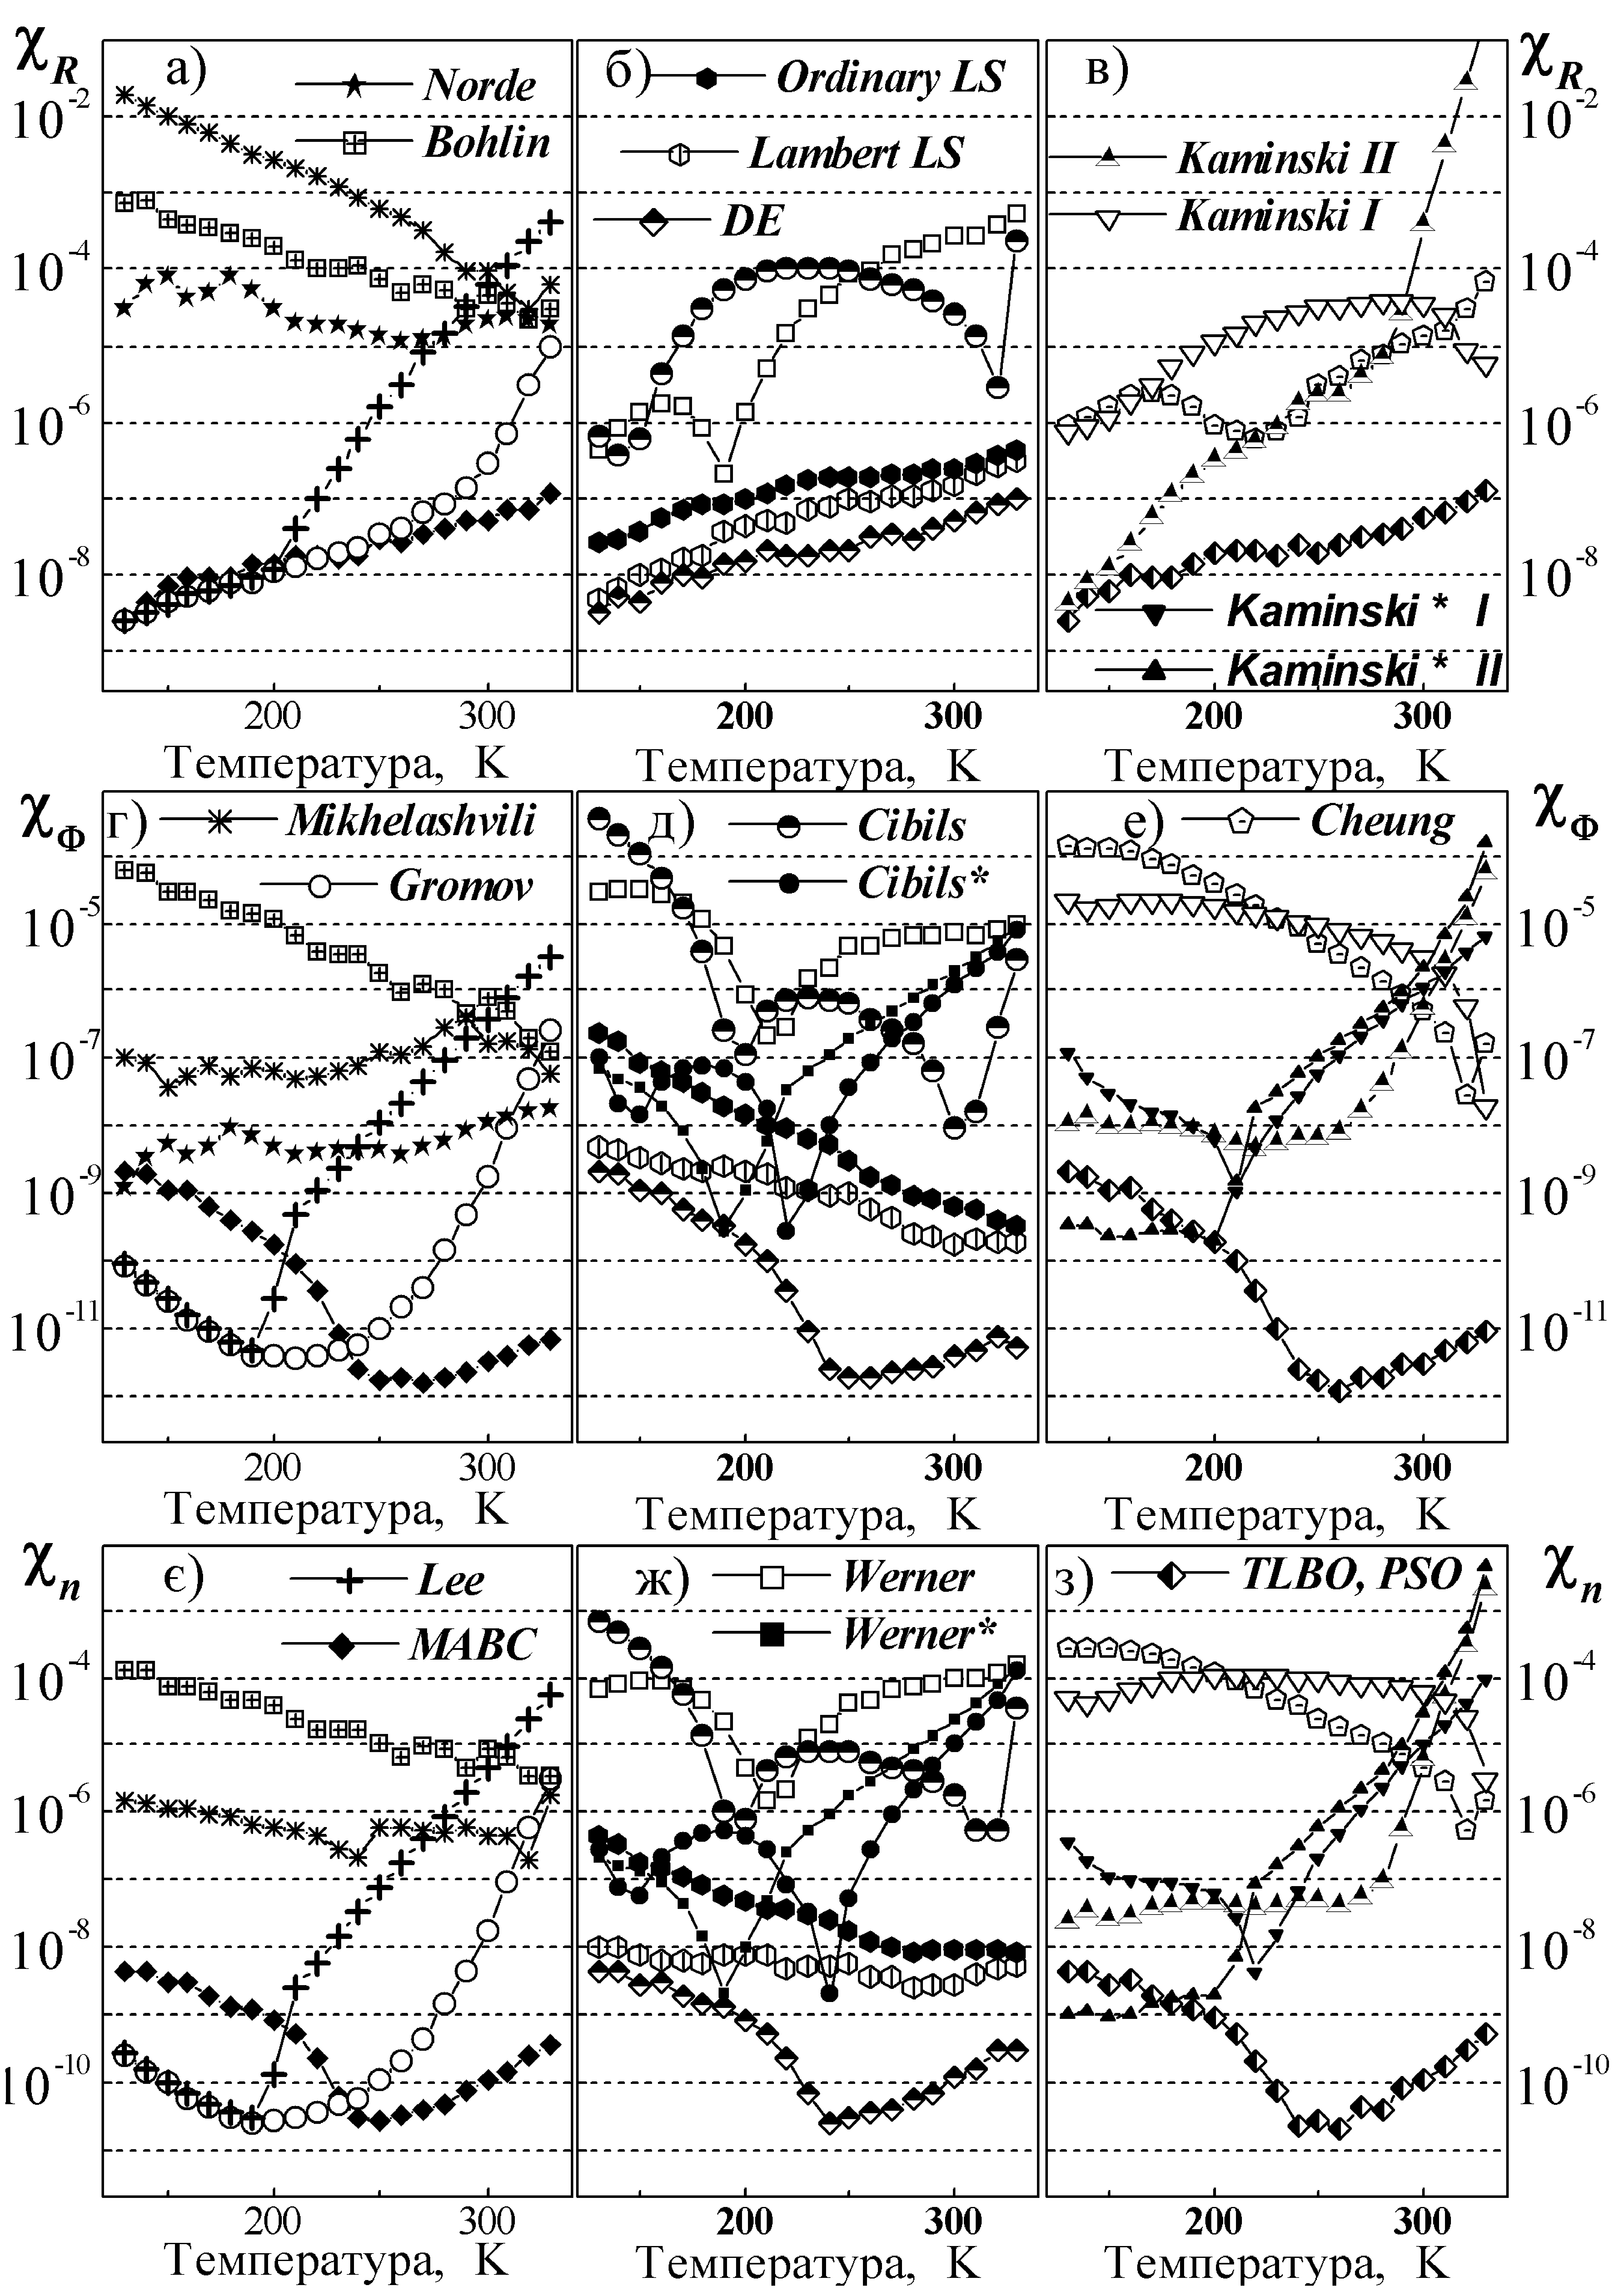
\includegraphics[width=0.85\textwidth]{figId}%
\caption{\label{figId}
Температурні залежності відносних похибок визначення $R_s$ (а --- в), $\Phi_b$ (г --- е) та $n_\mathrm{id}$ (є --- з) при застосуванні різних методів до ідеальних синтезованих ВАХ
%Залежності точності визначення послідовного опору (а --- в), ВБШ (г --- е) та фактора неідеальності (є --- з) при використанні різних методів від температури.
%Результати отримані при використанні ідеальних синтезованих ВАХ.
}
\end{figure}

Точність визначення параметрів із окремої ВАХ залежно від температури, для якої її синтезовано, наведено на рис.~\ref{figId}.
Насамперед зауважимо, що наведені дані показують:
\begin{enumerate}[label=\asbuk*),leftmargin=0em,itemindent=1.5em]
%\begin{enumerate}[label=\asbuk*),labelindent=0em,itemindent=1.5em]
\item при використанні всіх еволюційних алгоритмів для аналізу однакових ВАХ отримані дуже близькі значення як послідовного опору, так і ВБШ та фактора неідеальності;
це цілком очікуваних результат, пов'язаний з тим що у всіх випадках використовувалася ідентична цільова функція;
\item використання адаптивної процедури в методі Gromov дає можливість суттєво знизити помилки визначення параметрів;
\item використання функції Ламберта при числових обчисленнях дозволяє зменшити помилки визначення параметрів порівняно з випадком, коли в методі найменших квадратів використовується трансцендентна форма рівняння ВАХ;
\item при застосуванні методів Werner, Cibils, та Kaminskii~I за допомогою лінійної апроксимації допоміжної функції доцільно визначати лише величину послідовного опору,
тоді як $\Phi_b$ та $n_\mathrm{id}$ краще екстрагувати на наступному етапі, при лінійній апроксимацій ВАХ, скорегованої з врахуванням  отриманого значення $R_s$;
іншими словами використання варіантів цих методів, позначених зірочками дозволяє підвищити точність визначення параметрів;
\item найвищу точність при аналізі ідеальних синтезованих ВАХ вдається досягти при використанні еволюційних алгоритмів, апроксимації за допомогою методу найменших квадратів із використанням функції Ламберта, Norde (при визначенні $\Phi_b$), Ordinary LS (при визначенні $R_s$), методу Gromov, доповненого адаптивною процедурою, та методу Lee (за винятком випадків високих температур та великих значень $I_s$).
\end{enumerate}




\begin{figure}
\center
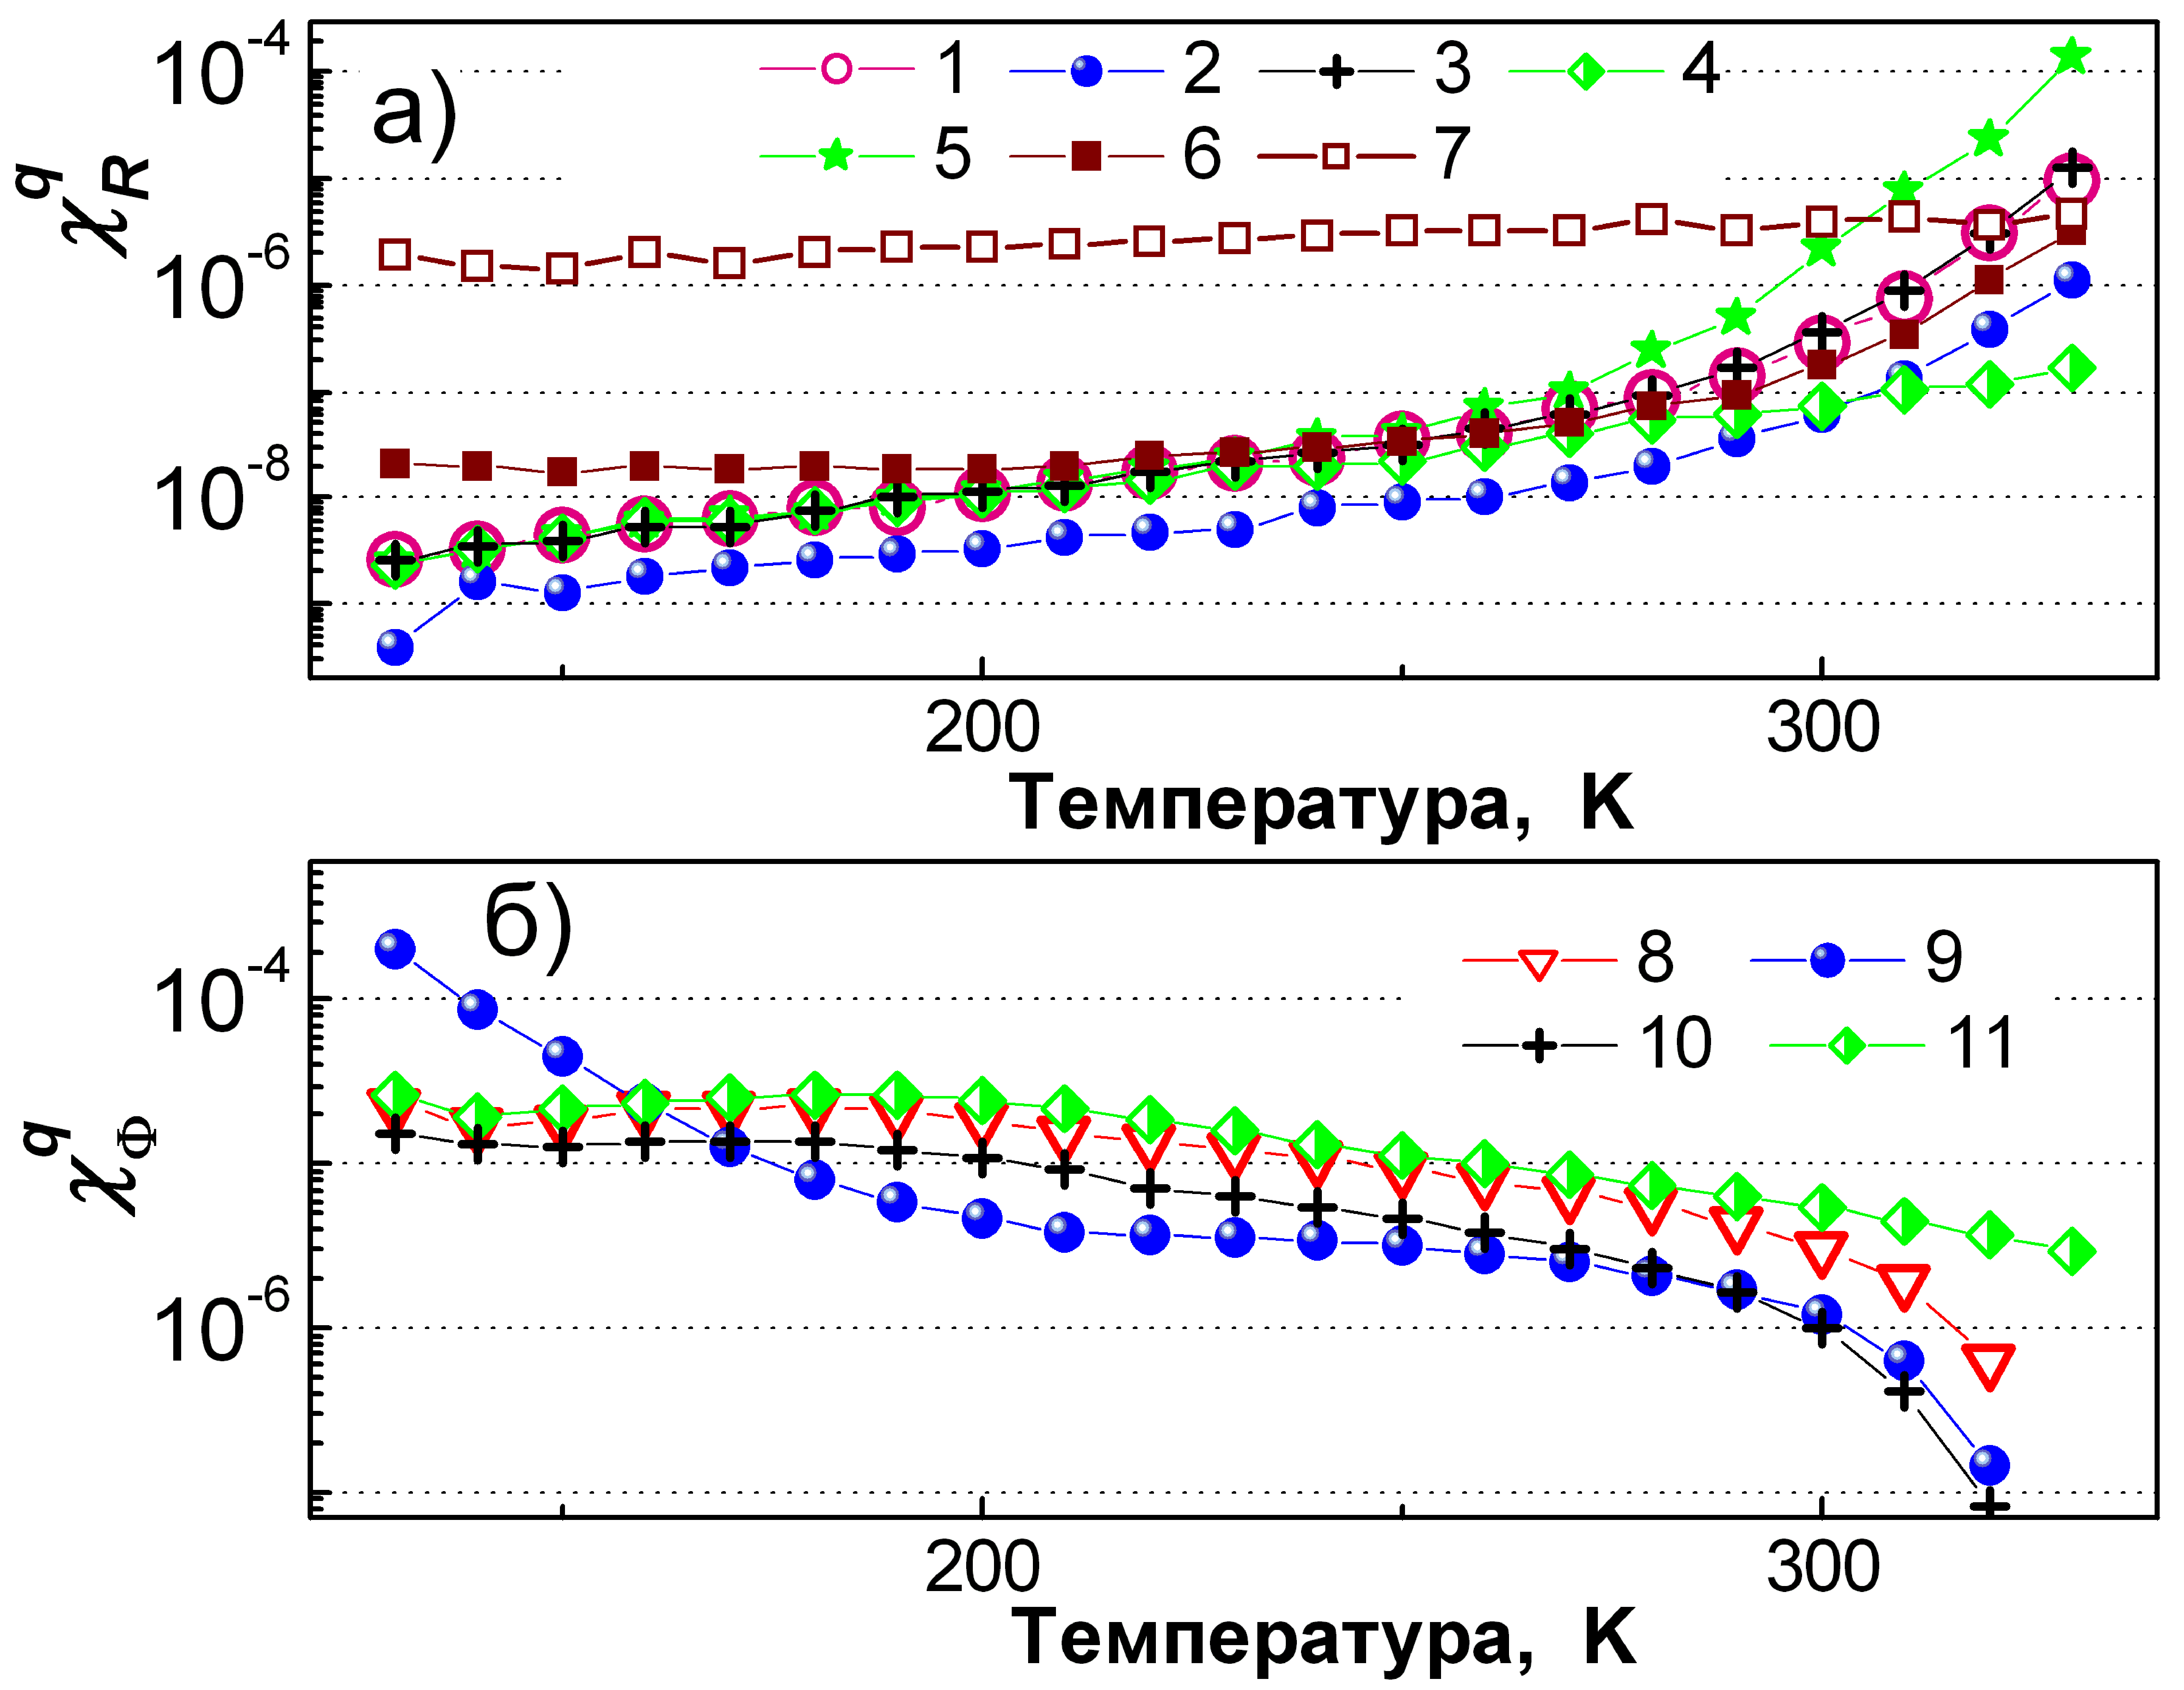
\includegraphics[width=0.65\textwidth]{figCon}%
\caption{\label{figCon}
Температурні залежності похибок визначення $R_s$ (a) та $\Phi_b$ (б) при використанні методів Gromov (a) та  Kaminskii I (б).
Під час синтезу ВАХ використовувалися параметри, величини яких переважно визначались формулами~(\ref{eqSDIs}--\ref{eqRsT}),
проте для  побудови кривих 2 та 9 використовувалися ВАХ для яких значення $R_s$ в 3 рази більше;
для кривих 3 та 10 величина $n_\mathrm{id}$  в 1,2 рази більша;
для кривих 4 та 11 величина $I_s$  в 100 разів менша;
для кривої 5 значення $\Phi_b$  зменшено на 0,1 еВ;
для кривої 6 величини $R_s$ та $\Phi_b$ залишалися незмінними та рівними 2~Ом та 0,7~еВ, відповідно, під час синтезу всього
набору ВАХ (були незалежні від температури);
для кривої 7 значення $R_s$ та $I_s$ незмінні та рівні 2~Ом та $10^{-5}$~A, відповідно
}
\end{figure}

З іншого боку, наведені результати показують, що точність визначення параметрів змінюється для різних ВАХ із одного набору (залежить від температури, для якої ВАХ була синтезована).
Тобто похибка визначення параметра з масиву $\left\{R_s\,,\,n_\mathrm{id}\,,\, I_s\right\}$ залежить як від його величини, так і від значення інших характеристик ДШ із цього набору.
Для виявлення подібних залежностей всі методи були також застосовані до синтезованих даних, при створенні яких вважалося, що одна з величин із набору ($R_s$, $\Phi_b$, $I_s$ $n_\mathrm{id}$) відрізняється за значенням від того, який очікується згідно з виразами ~(\ref{eqSDIs}--\ref{eqRsT}).
Окремі характерні результати наведені на рис.~\ref{figCon}.

Рис.~\ref{figCon},a свідчить що, похибки визначення послідовного опору при використанні методу Gromov
а)~зростають із підвищенням $\Phi_b$;
б)~зменшуються при збільшенні $R_s$ та зменшенні $I_s$;
в)~залишаються практично постійними при зміні $n_\mathrm{id}$.
%\begin{enumerate}[label=\asbuk*),leftmargin=0em,itemindent=1.5em]
%\item зростають з підвищенням $\Phi_b$;
%\item зменшуються при збільшенні $R_s$ та зменшенні $I_s$;
%\item залишаються практично постійними при зміні $n_\mathrm{id}$.
%\end{enumerate}
Очевидно, що $I_s$ та $\Phi_b$ пов'язані між собою співвідношенням~(\ref{eqSDIs}).
Проте, на нашу думку, саме величина струму насичення, а не ВБШ, є першочерговим фактором впливу на процес визначення $R_s$.
На користь цього висновку свідчать криві 6 та 7 на рис.~\ref{figCon},a.
Крива 6 отримана для набору ВАХ, які синтезовані використовуючи припущення що незалежними від температури є як $R_s$, так і $\Phi_b$.
Незважаючи на ці обмеження, $\chi^q_R$ зростає при збільшенні температури.
На противагу, крива 7, отримана для незалежних від температури $R_s$ та $I_s$, показує, що точність визначення послідовного опору залишається практично постійною для всього набору ВАХ.

З іншого боку, рис.~\ref{figCon},б показує, що при використанні методу Kaminskii I зменшення струму насичення підвищує похибку визначення ВБШ.
Загалом проведені дослідження показують, що величина $I_s$ є основним, а величина  $\Phi_b$ другорядним визначальними факторами для точності екстракції інших параметрів (не лише $R_s$) при використанні різних методів (не лише Gromov).
З рис.~\ref{figCon},б також видно, що похибка визначення $\Phi_b$ зменшується у випадку більших значень фактора неідеальності (криві 8 та 10).
Водночас збільшення послідовного опору немонотонно впливає на точність екстракції ВБШ (криві 8 та 9 на рис.~\ref{figCon},б):
при низьких температурах (високих значеннях $\Phi_b$) $\chi^q_{\Phi}$ зростає, при високих $T$ --- навпаки, зменшується.

Узагальнюючи аналіз отриманих результатів, можна зробити висновок, що точність визначення кожного з параметрів зазвичай зростає зі збільшенням його величини.
Проте похибка визначення $\chi^q_{x_i}$ даного параметра ($x_i\in\left\{R_s\,,\,n_\mathrm{id}\,,\, I_s\right\}$) залежить також і від абсолютних величин інших характеристик ДШ ($x_j,\,j\neq i$), причому характер цих залежностей є функцією абсолютних значень кожного параметра з набору і змінюється при використанні різних методів ($\chi^q_{x_i}=f(x_i,\,x_j,\,\text{метод})$).


\begin{figure}
\center
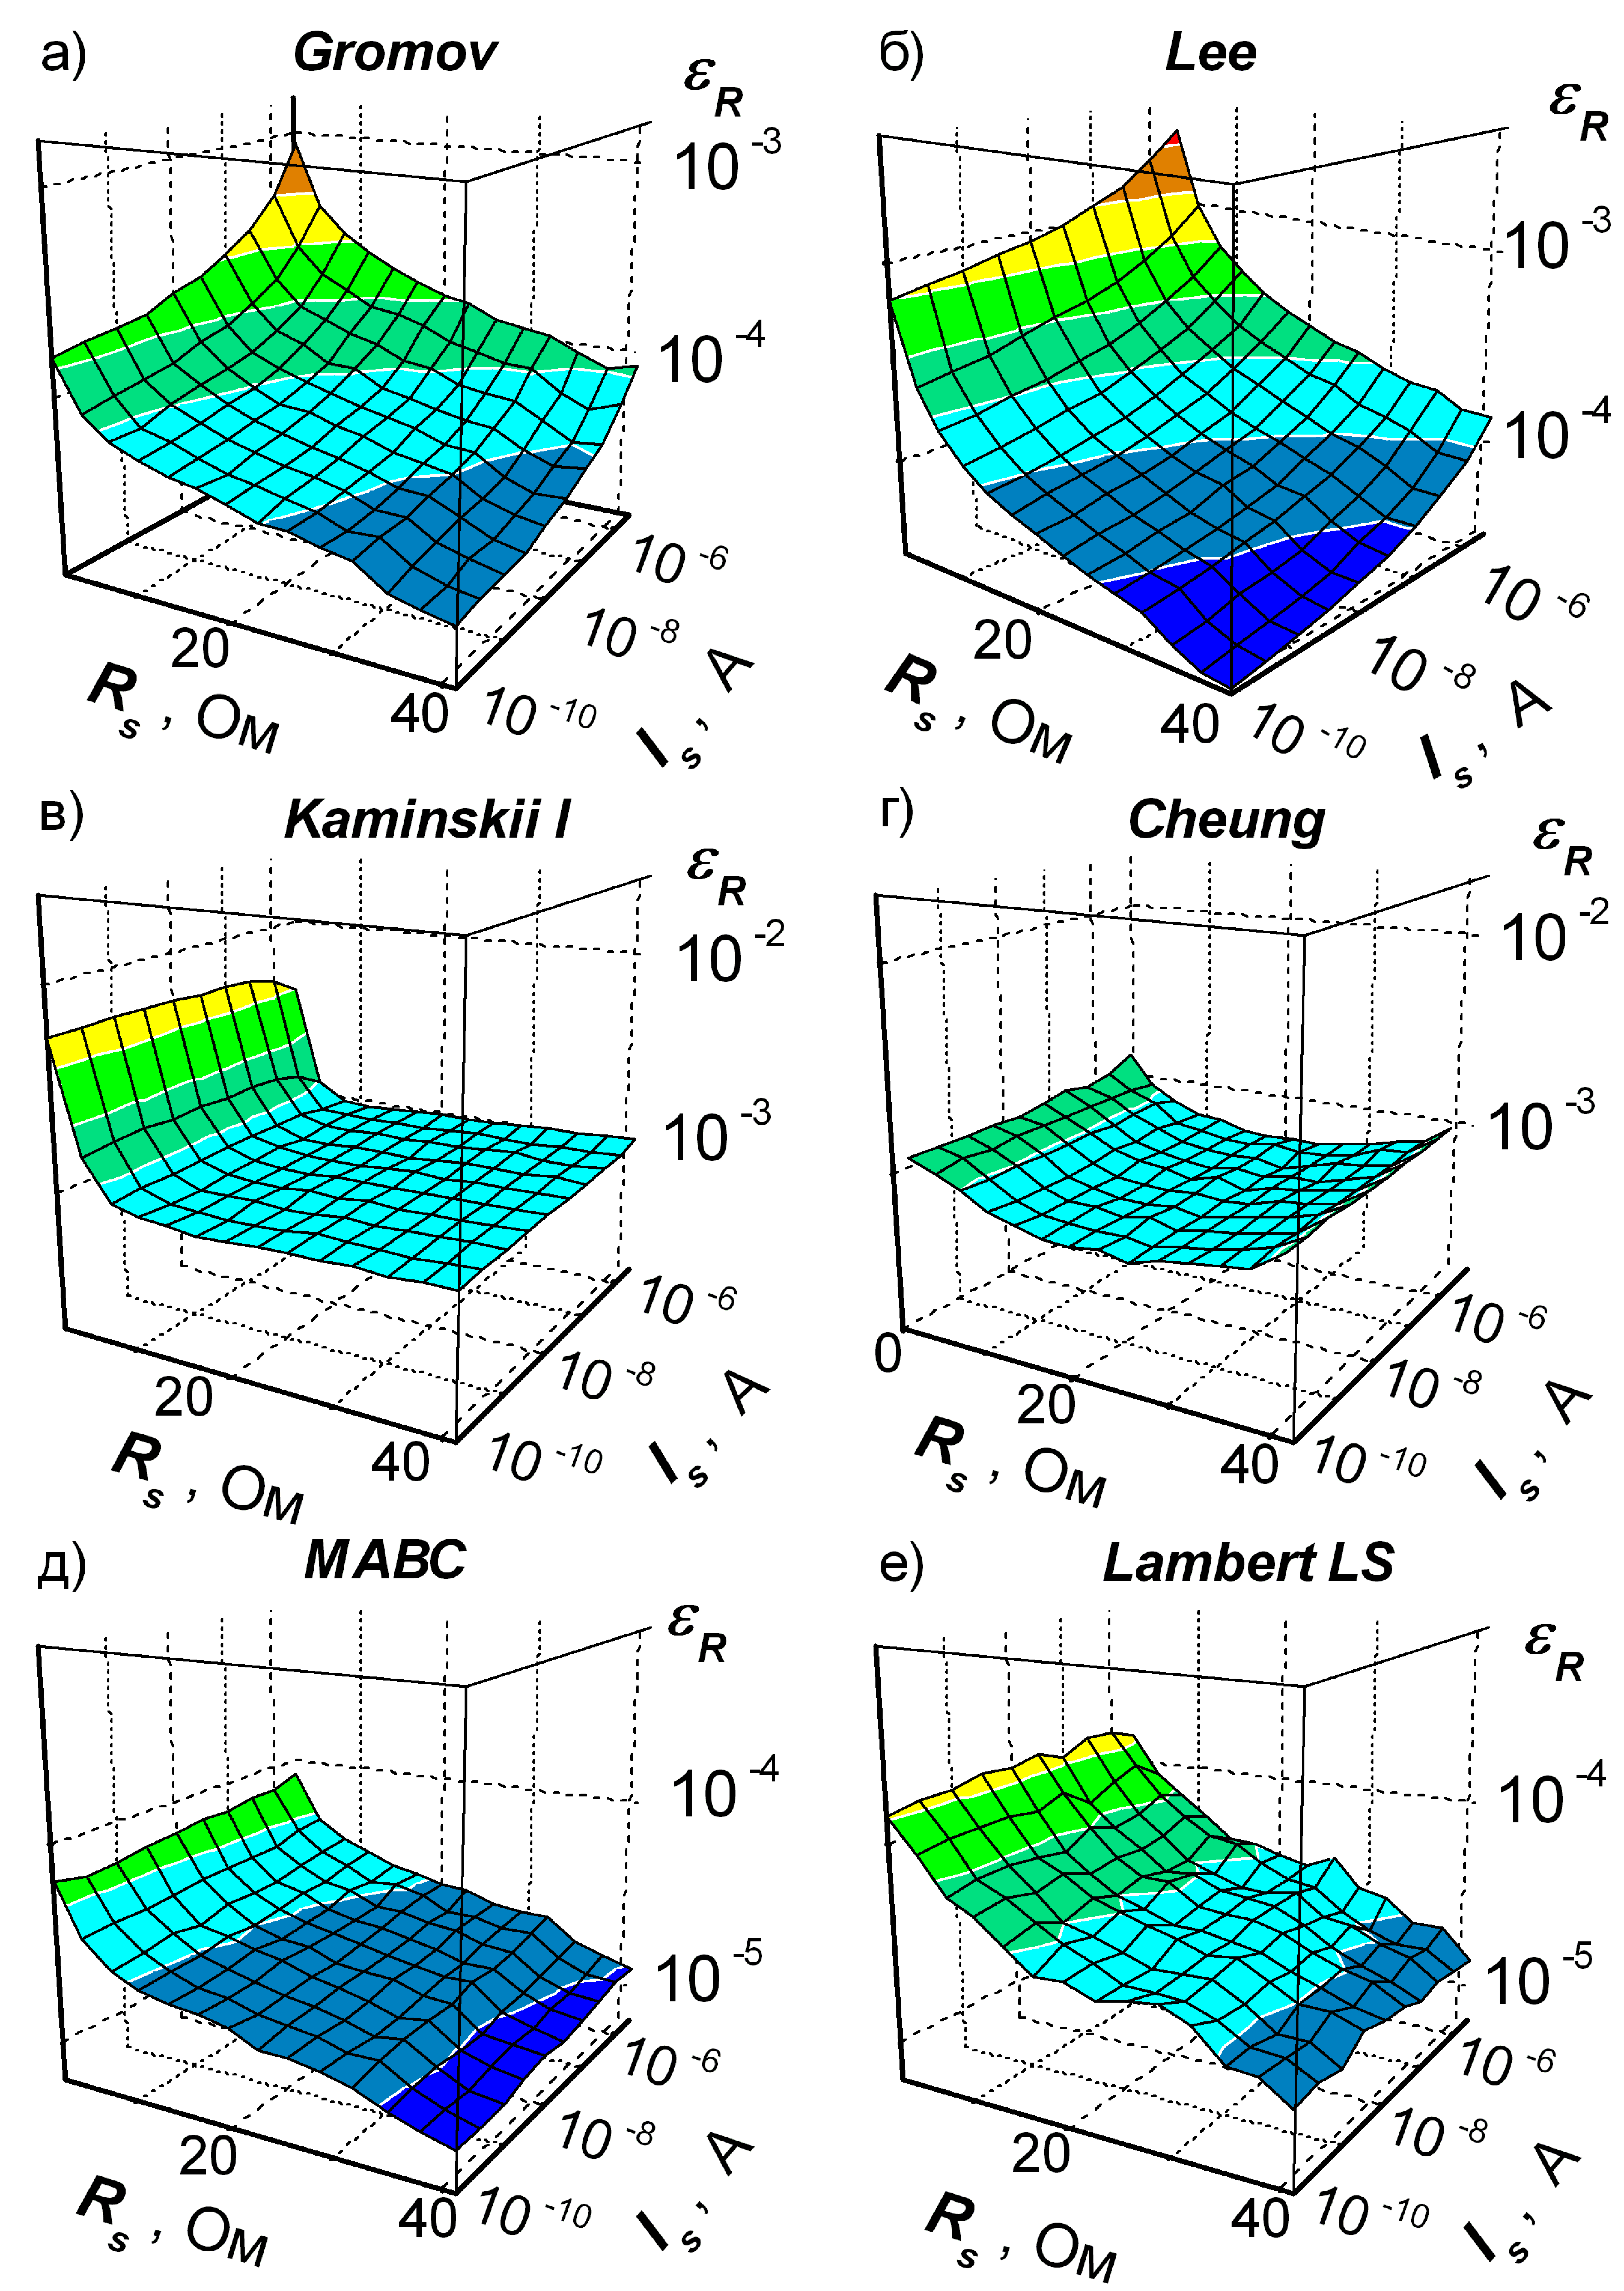
\includegraphics[width=0.8\textwidth]{figR3D}%
\caption{\label{figR3D}
Похибки визначення величини послідовного опору з набору ВАХ, який був синтезований при постійних значеннях $R_s$ та $I_s$.
Показані результати застосування методів Gromov (a), Lee (б), Kaminskii I (в), Cheung (г), MABC (д) та and Lambert LS (е)
}
\end{figure}

\begin{figure}
\center
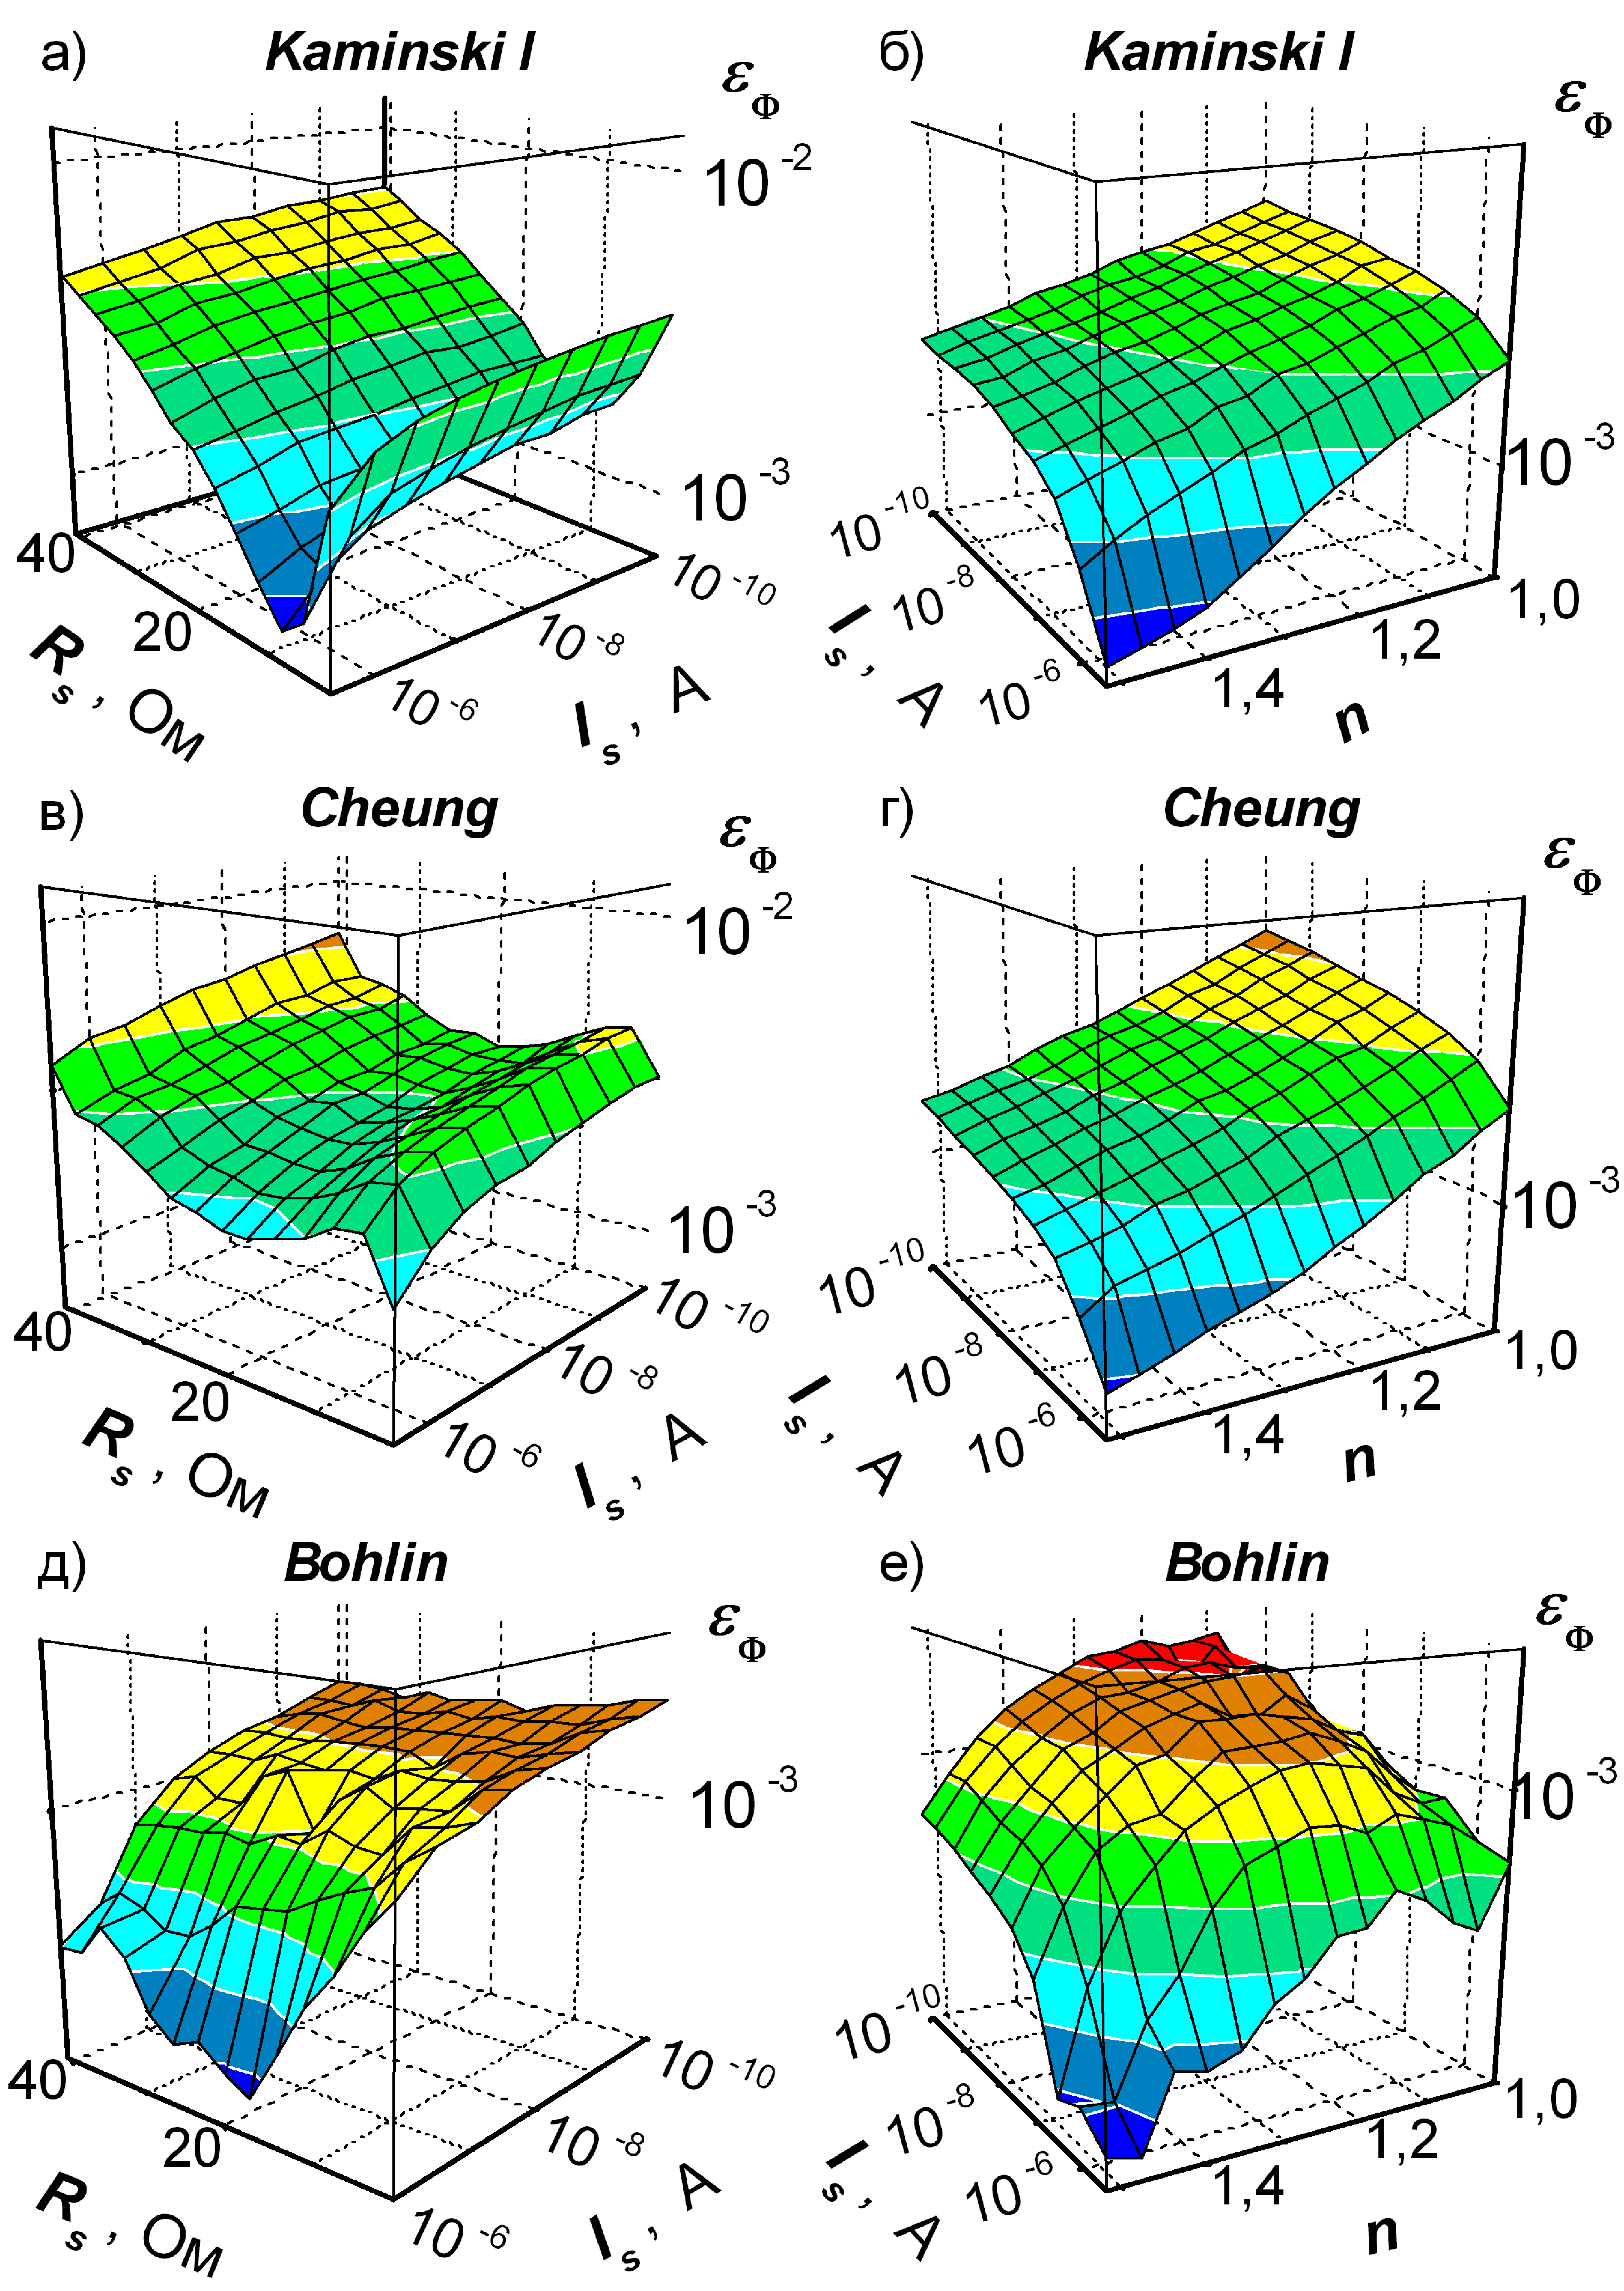
\includegraphics[width=0.8\textwidth]{figF3D}%
\caption{\label{figF3D}
Похибки визначення величини висоти бар'єру Шотткі опору з набору ВАХ, який був синтезований при постійних значеннях $R_s$ та $I_s$ (рисунки а, в та д) або постійних значеннях $n_\mathrm{id}$ та $I_s$ (рисунки б, г, е).
Показані результати застосування методів Kaminskii I (a, б), Cheung (в, г) та Bohlin (д, е)
}
\end{figure}


\begin{figure}
\center
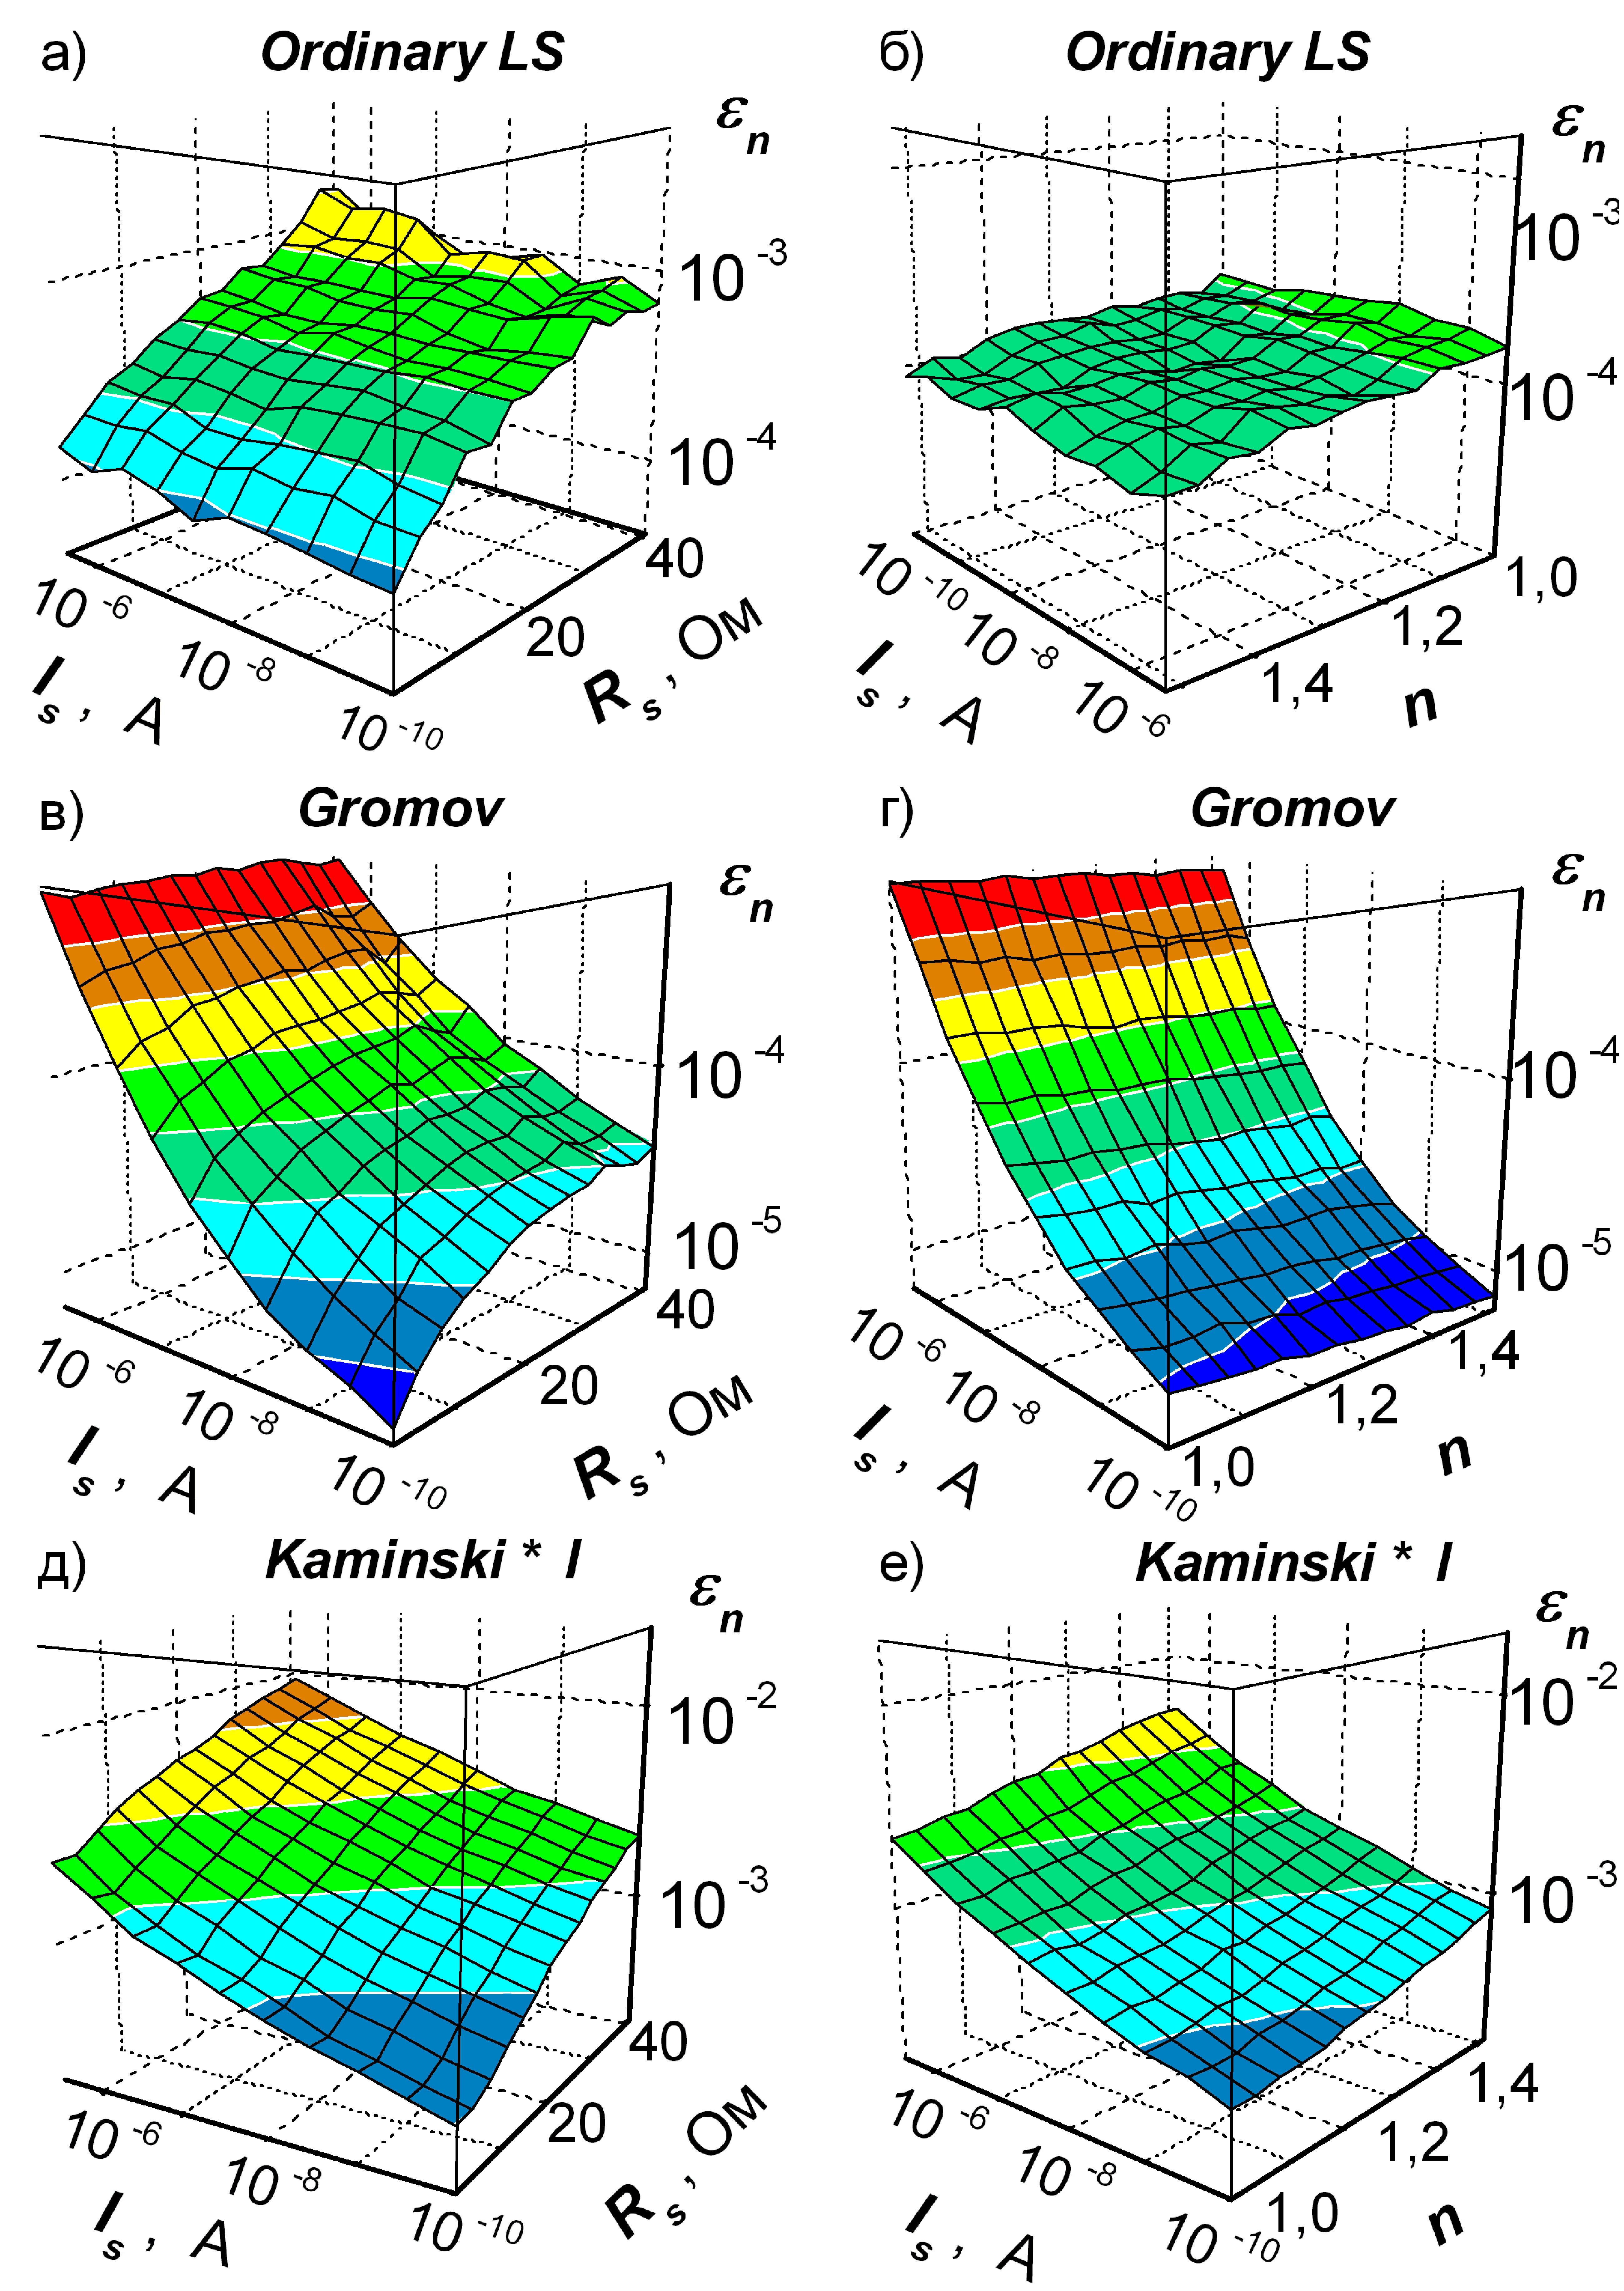
\includegraphics[width=0.8\textwidth]{fign3D}%
\caption{\label{fign3D}
Похибки визначення величини фактора неідеальності з набору ВАХ, який був синтезований при постійних значеннях $R_s$ та $I_s$ (рисунки а, в та д) або постійних значеннях $n_\mathrm{id}$ та $I_s$ (рисунки б, г, е).
Показані результати застосування методів Ordinary LS (a, б), Gromov (в, г) та Kaminskii*~I (д, е)
}
\end{figure}

Для того, щоб виявити основні тенденції цих залежностей проведені додаткові числові дослідження.
А саме, були синтезовані набори ВАХ, при побудові яких вважалося, що окремі параметри є незалежними від температури.
При цьому
а)~постійними у всьому температурному діапазоні вважалася два параметри ($R_s$ та $I_s$  або $n_\mathrm{id}$ та $I_s$ для різних наборів ВАХ);
б)~$n_\mathrm{id}$ (або $R_s$) обчислювалися відповідно до того, як описано раніше, в розділі~\ref{SubData}.
Було створено сукупність наборів ВАХ, для яких незалежні від температури величини $R_s$, $n_\mathrm{id}$ та $I_s$ змінювались в діапазонах від
2 до 41~Ом, від 1 до 1,52 та від $10^{-10}$ до $5\cdot10^{-5}$~A, відповідно.
Після цього кожний із методів застосовувався до кожного набору ВАХ, визначено величини параметрів, а також їхні похибки.
Найтиповіші результати наведено на рис.~\ref{figR3D}--\ref{fign3D}.
Зокрема, рис.~\ref{figR3D},a підтверджує, що при використанні методу Gromov збільшення $R_s$ та $I_s$ призводить до зменшення та збільшення помилки визначення послідовного опору, відповідно.


Отримані результати щодо факторів впливу узагальнено в табл.~\ref{tabIF}.
У таблиці використано ряд символів для опису поведінки похибки визначення параметрів при зміні величини фактора впливу.
А саме.
Якщо помилка визначення монотонно зростає або зменшується зі збільшенням впливаючого фактора, то використовувалися символи <<$\downarrow$>> та <<$\uparrow$>>, відповідно.
Наприклад, саме ці символи характеризують кореляцію точності визначення $R_s$ за допомогою методу Gromov та величини $R_s$ та $I_s$.
Виявлено, що точність визначення може залежати від фактора впливу не лише монотонно.
Наприклад, рис.~\ref{figCon},б та рис.~\ref{figF3D},a показують, що при використанні методу Kaminskii~I похибка визначення $\Phi_b$ зростає з підвищенням послідовного опору при великих ($>10$~Ом) значеннях $R_s$ і зменшується при малих величинах $R_s$.
Для позначення залежності з такою поведінкою в табл.~\ref{tabIF} використовується символ <<$\vee$>>.
Подібна залежність спостерігається при використанні метода Chueng для визначення $R_s$ (рис.~\ref{figR3D},г).
Проте в цьому випадку сама величина $R_s$ порівняно слабко впливає на точність визначення послідовного опору.
Схожі слабкі залежності позначаються в табл.~\ref{tabIF} за допомогою верхнього індексу  <<$w$>>.
Інші приклади слабких залежностей $I_s$ та  $n_\mathrm{id}$ можна побачити на рис.~\ref{figR3D},д та рис.~\ref{fign3D},г, відповідно.


\begin{table}
\caption{\label{tabIF}Фактори впливу на похибки визначення параметрів ДШ$^{1)}$
%\footnote{The presence of $R_s$ or $I_s$ or $n$ in the cell indicates the impact on extracted parameter accuracy;
%the subscript and inside bracket symbol deal with extraction error behavior with influencing factor increasing --- see details in the text.}
}
\centering
\small
\begin{tabular}{|l|c|c|c|}
%\begin{tabularx}{\textwidth}{|l|
%                              >{\centering\arraybackslash}X|
 %                             >{\centering\arraybackslash}X|
  %                            >{\centering\arraybackslash}X|}
\hline
\multicolumn{1}{|c|}{Метод}&\multicolumn{3}{c|}{Визначений параметр}\\
\cline{2-4}
%\hline
 &$R_s$&$\Phi_b$&$n$\\
%Метод &$R_s$&$\Phi_b$&$n$\\
%\hline
%\hline
\hhline{|====|}
Norde &$n_\mathrm{id}^w(\vee)$&$I_s(\downarrow)$&---\\
\hline
Werner &$R_s(\vee)$&$R_s(\downarrow)$, $I_s^w(\downarrow)$, $n_\mathrm{id}^w(\downarrow)$&$R_s(\uparrow)$, $n_\mathrm{id}^w(\downarrow)$\\
\hline
Werner* &$R_s(\vee)$&$R_s(\vee)$, $I_s(\uparrow)$, $n_\mathrm{id}(\uparrow)$&$R_s(\vee)$, $I_s(\uparrow)$, $n_\mathrm{id}^w(\uparrow)$\\
\hline
Cibils &$R_s(\vee)$, $n_\mathrm{id}(\uparrow)$&$R_s(\uparrow)$, $n_\mathrm{id}(\vee)$& $R_s(\uparrow)$, $n_\mathrm{id}(\vee)$\\
\hline
Cibils* &$R_s(\vee)$, $n_\mathrm{id}(\uparrow)$&$R_s(\vee)$, $I_s(\uparrow)$, $n_\mathrm{id}(\uparrow)$& $R_s(\vee)$, $I_s(\uparrow)$, $n_\mathrm{id}(\uparrow)$\\
\hline
Kaminskii I&$R_s(\leftharpoonup)$, $n_\mathrm{id}^w(\downarrow)$&$R_s(\vee)$, $I_s(\downarrow)$, $n_\mathrm{id}(\downarrow)$& $R_s(\vee)$, $I_s^w(\downarrow)$, $n_\mathrm{id}(\downarrow)$\\
\hline
Kaminskii* I&$R_s(\leftharpoonup)$, $n_\mathrm{id}^w(\downarrow)$&$R_s(\uparrow)$, $I_s(\uparrow)$, $n_\mathrm{id}(\uparrow)$& $R_s(\uparrow)$, $I_s(\uparrow)$, $n_\mathrm{id}(\uparrow)$\\
\hline
Kaminskii II&$R_s(\downarrow)$, $I_s(\rightharpoonup)$, $n_\mathrm{id}^w(\uparrow)$&$I_s(\rightharpoonup)$, $n_\mathrm{id}^w(\uparrow)$& $I_s(\rightharpoonup)$\\
\hline
Kaminskii* II&$R_s(\downarrow)$, $I_s(\rightharpoonup)$, $n_\mathrm{id}^w(\uparrow)$&$I_s(\uparrow)$, $n_\mathrm{id}(\uparrow)$& $I_s(\uparrow)$, $n_\mathrm{id}(\uparrow)$\\
\hline
Bohlin &$I_s(\rightharpoondown)$&$I_s(\downarrow)$, $n_\mathrm{id}(\wedge)$& $I_s(\rightharpoondown)$, $n_\mathrm{id}(\wedge)$\\
\hline
Lee &$R_s(\downarrow)$, $I_s(\uparrow)$, $n_\mathrm{id}(\uparrow)$&$I_s(\uparrow)$, $n_\mathrm{id}(\uparrow)$& $I_s(\uparrow)$, $n_\mathrm{id}(\uparrow)$\\
\hline
Gromov &$R_s(\downarrow)$, $I_s(\uparrow)$&$R_s(\uparrow)$, $I_s(\uparrow)$, $n_\mathrm{id}^w(\downarrow)$&$R_s(\uparrow)$, $I_s(\uparrow)$, $n_\mathrm{id}^w(\downarrow)$\\
\hline
Cheung &$R_s^w(\vee)$&$R_s(N)$, $I_s(\downarrow)$, $n_\mathrm{id}(\downarrow)$&$R_s^w(N)$, $I_s(\rightharpoondown)$, $n_\mathrm{id}(\downarrow)$\\
\hline
Mikhelashvili &$R_s(\uparrow)$, $I_s(\downarrow)$, $n_\mathrm{id}^w(\downarrow)$&$R_s(\uparrow)$, $I_s(\wedge)$, $n_\mathrm{id}^w(\downarrow)$&$R_s(\uparrow)$, $I_s(\wedge)$, $n_\mathrm{id}^w(\downarrow)$\\
\hline
Ordinary LS &$R_s(\downarrow)$&$R_s(\uparrow)$, $I_s^w(\downarrow)$, $n_\mathrm{id}^w(\downarrow)$&$R_s(\uparrow)$, $n_\mathrm{id}^w(\downarrow)$\\
\hline
Lambert LS &$R_s(\downarrow)$&$I_s^w(\downarrow)$&$n_\mathrm{id}^w(\downarrow)$\\
\hline
EAs &$R_s(\downarrow)$, $I_s^w(\uparrow)$&$R_s(\uparrow)$, $I_s(\vee)$, $n_\mathrm{id}^w(\downarrow)$&$R_s(\uparrow)$, $I_s(\vee)$, $n_\mathrm{id}^w(\downarrow)$\\
\hline
\multicolumn{4}{p{0.9\textwidth}}{$^{1}$\textit{Наявність $R_s$ або $I_s$ або $n_\mathrm{id}$ в клітинці означає
вплив величини, відповідно, послідовного опору або струму насичення або фактора неідеальності на точність визначення параметра;
верхній індекс та символ в дужках пов'язані з характером поведінки точності визначення параметра при збільшенні $R_s$ або $I_s$ або $n_\mathrm{id}$ --- деталі див. у тексті.
}}\\
%\hline
\end{tabular}
%\end{tabularx}
\end{table}



Якщо графік залежності похибки визначення параметра від величини фактора впливу має не мінімум, а максимум (див., наприклад, рис.~\ref{figF3D},е),
то використовувався символ <<$\wedge$>>.
Наявність на залежності екстремумів обох типів (див., наприклад, рис.~\ref{figF3D},в) позначено за допомогою символу <<$N$>>.

Ще один тип залежності показаний на рис.~\ref{figR3D},в.
При використанні методу Kaminskii~I для визначення  $R_s$ помилки залишаються постійними в широкому діапазоні змін $R_s$ та $I_s$ і зростають лише для малих значень $R_s$.
Подібні залежності між помилкою визначення та впливаючим фактором позначені символом <<$\leftharpoonup$>>.
Символи <<$\rightharpoonup$>> або <<$\rightharpoondown$>> використовуються, якщо помилки зростають або зменшуються, відповідно, лише при великих значеннях фактора впливу.

З наведених даних, зокрема, видно, що фактори, які впливають на точність екстракції $\Phi_b$ та  $n_\mathrm{id}$ подібні для більшості методів, які розглядалися в роботі.
Використання адаптивної процедури в методі Gromov призводить до того, що точність визначення $\Phi_b$ та  $n_\mathrm{id}$ стає залежною від величини $R_s$, тоді як вплив величини фактора неідеальності послаблюється.
Точність методів Werner*, Cibils* та Kaminskii* чутливіша до величин параметрів ніж при використанні варіантів цих же методів без зірочок.
Найстійкішими до величин параметрів є числові методи, особливо при використанні функції Ламберта (Lambert LS).


\subsection{Швидкодія методів визначення параметрів діодів Шотткі}
Ще одним, поряд із точністю, критерієм для характеризації різних методів визначення параметрів структур МН є час, необхідний для розрахунків (RT, running time).
Для оцінки RT  використані WinAPI функції $QueryPerformanceCounter()$ та $QueryPerformanceFrequency()$.
Розрахунки проводились на персональному комп'ютері з наступними характеристиками:
\begin{itemize}[leftmargin=0em,itemindent=1.5em]
  \item процесор AMD A4-3400 2.7~GHz;
  \item 3072~MB RAM;
  \item операційна система Windows XP.
\end{itemize}
Очевидно, що точний час екстракції параметрів залежить від програмної реалізації, від завантаження процесора в даний момент часу тощо.
Тим не менш, всі методи тестувалися за однакових умов, а отже вибраний підхід дозволяє порівняти тривалість роботи різних методів, а також оцінити порядок величини RT.

\begin{table}
\caption{\label{tabRT}Час визначення параметрів ДШ з однієї ВАХ}
\begin{tabularx}{\textwidth}{|>{\raggedright\arraybackslash}X|
                             >{\centering\arraybackslash}X|
                            >{\centering\arraybackslash}X|}
\hline
\multicolumn{1}{|c|}{Метод}&\multicolumn{2}{c|}{Час роботи, с}\\
\cline{2-3}
%\begin{tabular}{lcc}
%Method &\multicolumn{2}{c}{Running time, s}\\
 &максимальний&мінімальний\\
\hhline{|===|}
Norde &$3,7\cdot10^{-5}$&$2,6\cdot10^{-5}$\\ \hline
Werner $^{1)}$ &$4,5\cdot10^{-5}$&$4,0\cdot10^{-5}$\\ \hline
Cibils $^{1)}$ &$5,3\cdot10^{-3}$&$1,9\cdot10^{-4}$\\ \hline
Kaminskii I $^{1)}$ &$8,0\cdot10^{-5}$&$4,5\cdot10^{-5}$\\ \hline
Kaminskii II $^{1)}$ &$2,6\cdot10^{-3}$&$3,0\cdot10^{-4}$\\ \hline
Bohlin &$6,3\cdot10^{-5}$&$4,0\cdot10^{-5}$\\ \hline
Lee &$3,6\cdot10^{-3}$&$1,8\cdot10^{-4}$\\ \hline
Gromov &$2,2\cdot10^{-2}$&$2,2\cdot10^{-2}$\\ \hline
Gromov $^{2)}$ &$4,6\cdot10^{-5}$&$2,7\cdot10^{-5}$\\ \hline
Cheung &$3,2\cdot10^{-5}$&$2,0\cdot10^{-5}$\\ \hline
Mikhelashvili &$4,7\cdot10^{-5}$&$2,9\cdot10^{-5}$\\ \hline
Ordinary LS &$460$&$1,8$\\ \hline
Lambert LS &$540$&$7,6$\\ \hline
DE &$0,73$&$0,36$\\ \hline
PSO &$0,35$&$0,14$\\ \hline
MABC &$0,20$&$5,7\cdot10^{-2}$\\ \hline
TLBO &$19,2$&$5,4$ \\
\hline
\multicolumn{3}{p{17cm}}{$^{1}$\textit{Час корекції ВАХ та лінійної апроксимації дорівнює $1.8\cdot10^{-5}$~с (максимальний) або $1.4\cdot10^{-5}$~с (мінімальний)}.
}\\
\multicolumn{3}{p{17cm}}{$^{2}$\textit{Для випадку, коли адаптивна процедура не використовується}.
}\\ %\hline
\end{tabularx}
\end{table}

Отримані значення RT при застосуванні різноманітних методів до аналізу ідеальних синтезованих ВАХ наведено в табл.~\ref{tabRT}.
Загалом RT залежить від кількості точок у вихідній залежності;
в таблиці наведено значення, отримані при застосування методів до ВАХ, сгенерованих для температур 130~K та 330~K.
Очевидно, що
\begin{enumerate}[label=\asbuk*),leftmargin=0em,itemindent=1.5em]
\item час роботи аналітичних методів при використанні сучасних комп'ютерів знехтувано малий;
\item у випадку ВАХ із великою кількістю експериментальних точок RT числових методів може досягати значних величин;
\item використання функції Ламберта призводить до збільшення часу роботи числових методів; однією з причин цього є необхідність використовувати числовий ряд для обчислення значення самої функції;
\item використання адаптивної функції очікувано викликає збільшення RT на декілька порядків, проте його абсолютне значення залишається невеликим;
\item серед еволюційних алгоритмів найшвидшим при визначенні параметрів ДШ є MABC, тоді як найповільнішим --- TLBO.
\end{enumerate}


Узагальнюючи результати, отримані при дослідженні застосування методів до ідеальних синтезованих ВАХ, зауважимо,
що еволюційні алгоритми видаються найпридатнішими для визначення параметрів ДШ завдяки низькому рівню помилок, помірній чутливості точності до величини параметрів
та допустимому часу роботи.
Поряд із цим, іншими методами, яким також варто надавати перевагу є аналітичний метод Gromov із використанням адаптивної процедури та числовий метод Lambert LS.
Проте точність визначення параметрів для першого з них суттєво зменшується при високих значеннях струму насичення (високих температурах).
Щодо методу Lambert LS, то його основним недоліком є значний час, потрібний для обчислень.


\subsection{Вплив випадкових похибок на точність визначення параметрів структур метал---напівпровідник}

На рис.~\ref{figG1003} та рис.~\ref{figDiag} наведено результати застосування різноманітних методів до зашумлених даних.
Цілком очікувано, помилки при екстракції параметрів збільшуються при підвищенні рівня шуму (рівня випадкових помилок при вимірюванні).
Проте залежності правильності визначення параметрів із однієї ВАХ схожі до отриманих при аналізі ідеальних синтезованих ВАХ.
Як наслідок, фактори впливу на точність також ідентичні, тобто дані табл.~\ref{tabIF} цілком застосовні і в цьому випадку.
Інші характерні особливості методів, виявлені раніше, проявляються і в цьому випадку.
Наприклад, використання функції Ламберта дозволяє досягнути більшої точності числових методів при визначенні параметрів ДШ.
Еволюційні алгоритми, методи Gromov та Lee характеризуються найменшими помилками.
Водночас, різниця між результатами, отриманими за допомогою методів Gromov та Lee зменшується.
Це свідчить про зниження переваги застосування запропонованої адаптивної процедури з підвищенням рівня випадкових похибок.



\begin{figure}
\center
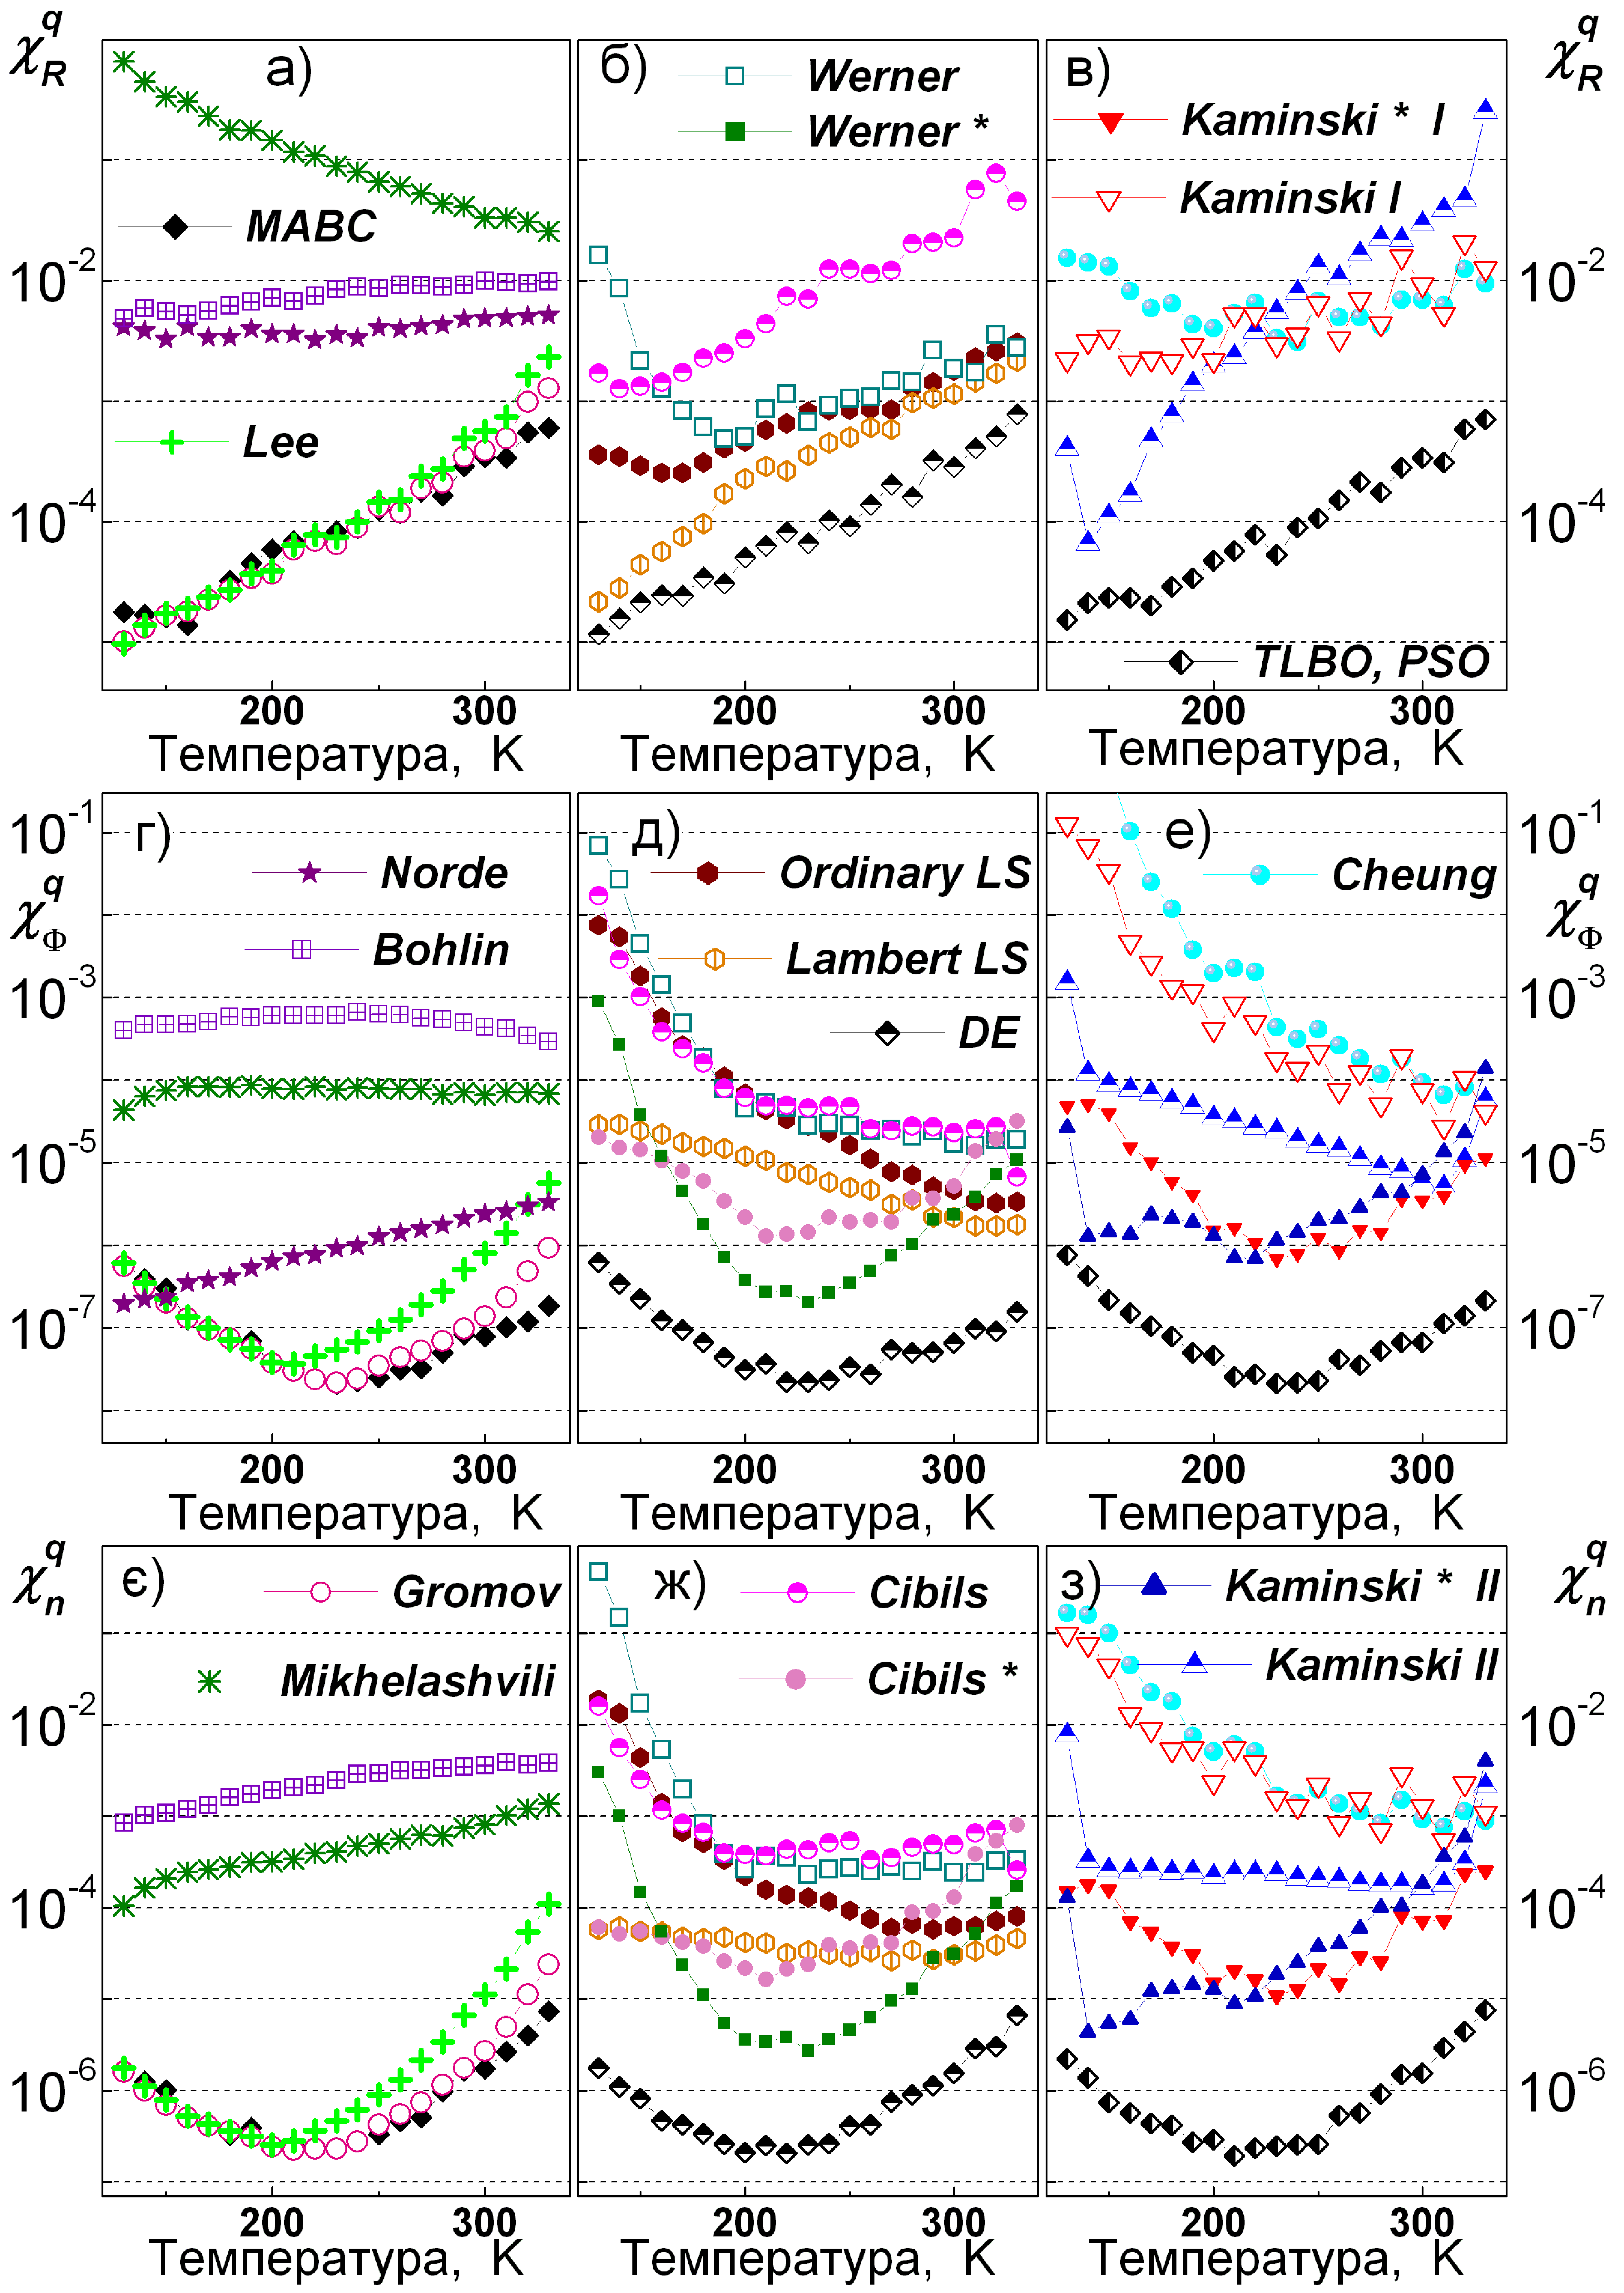
\includegraphics[width=0.8\textwidth]{figG1003}%
\caption{\label{figG1003}
Температурні залежності похибок визначення послідовного опору (а --- в), ВБШ (г --- е) та фактора неідеальності (є --- з) при застосуванні різних методів до наборів зашумлених даних.
$\sigma_V=0,3$~мВ, $\sigma_I^\varepsilon=1\%$
}
\end{figure}

\begin{figure}
\center
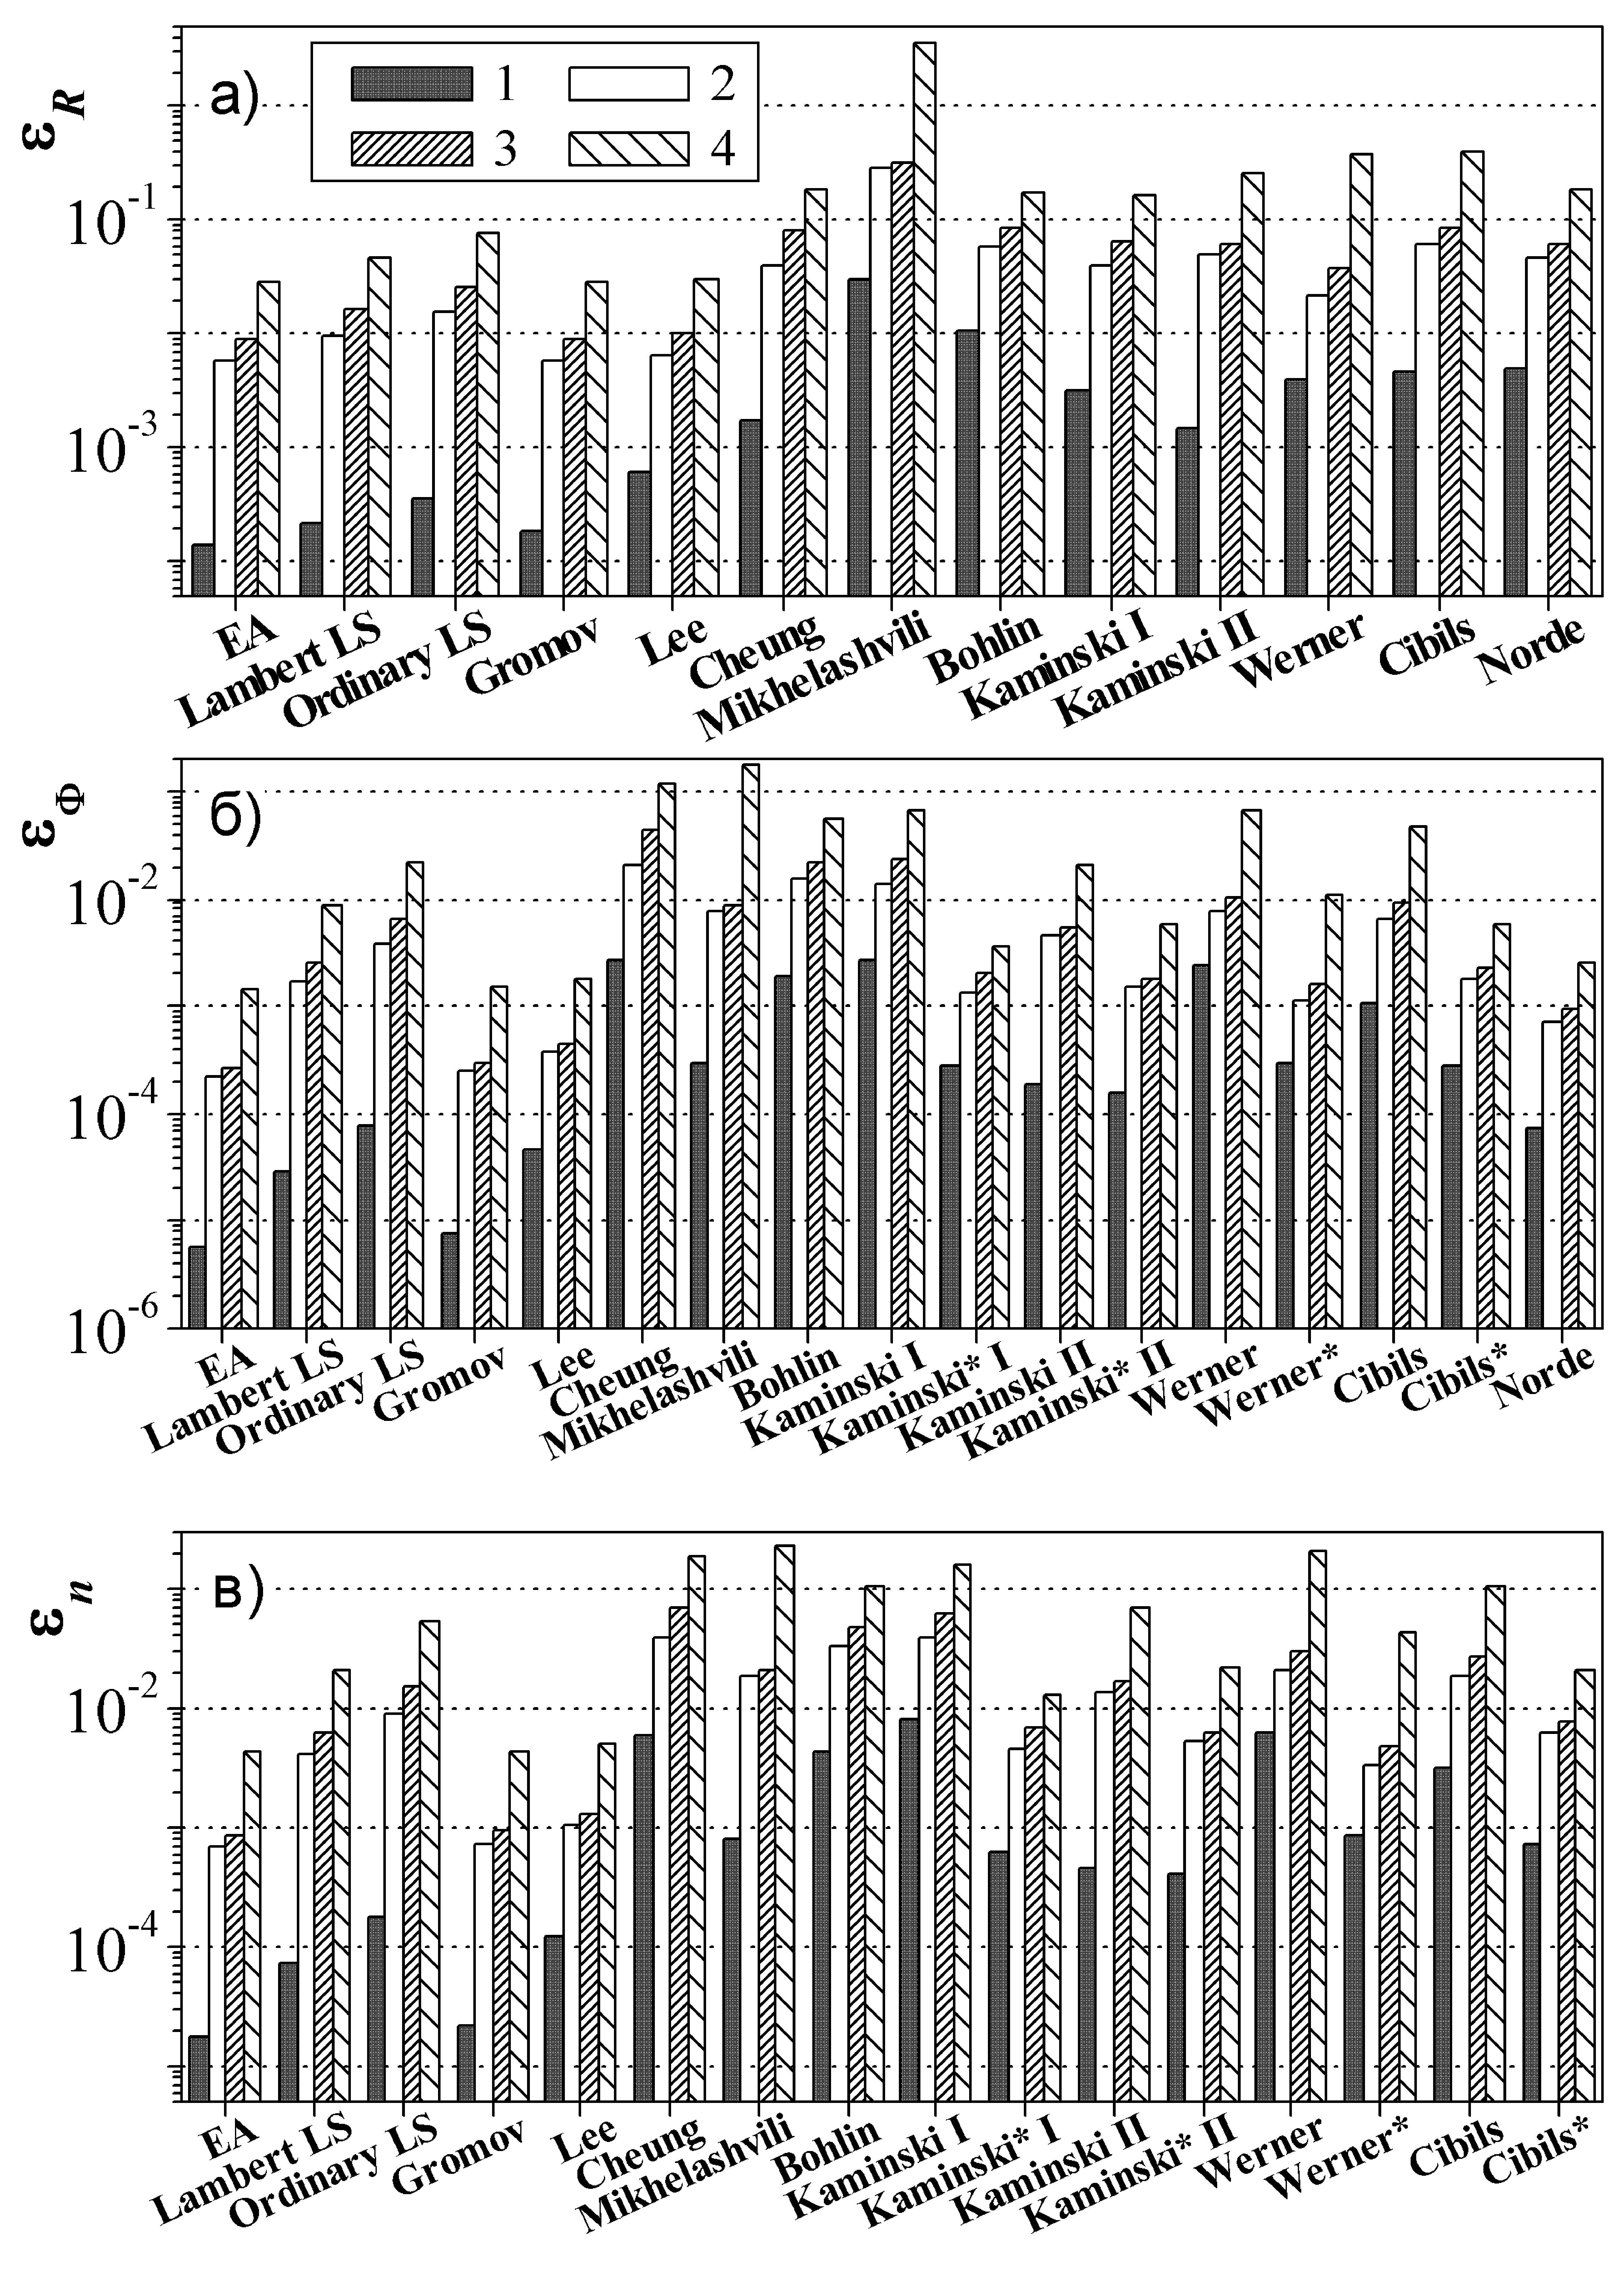
\includegraphics[width=0.8\textwidth]{figDiag}%
\caption{\label{figDiag}
Похибки визначення $R_s$ (a), $\Phi_b$ (б) та $n_\mathrm{id}$ (в) з наборів зашумлених даних.
$\sigma_V$, мВ: 0 (1), 0,3 (2, 3), 2 (4).
$\sigma_I^\varepsilon$, \%: 0 (1), 0,5 (2), 1 (3, 4)
}
\end{figure}


У випадку, коли методи Werner, Cibils, Kaminskii~I або  Kaminskii~IІ застосовуються до зашумлених даних, визначення $n_\mathrm{id}$ шляхом апроксимації скорегованої ВАХ є точнішим, ніж у випадку, коли ця величина визначається внаслідок апроксимації допоміжної функції.
Крім того, точність цих методів наближається до найкращих результатів інших методів і стає порівняною з точністю числових методів, або й навіть переважає її (рис.~\ref{figG1003}).
Метод Norde дозволяє достатньо точно визначати висоту бар'єру Шотткі, проте фактор неідеальності можна отримати лише застосовуючи інші методи.

Залежності похибок визначення параметрів від рівня шуму (від рівня випадкових помилок) показані на рис.~\ref{figErr}.
Наведені графіки отримані при використанні методу Gromov, проте вони є цілком типовими і для інших методів.
Видно, що величини помилок при визначенні всіх параметрів практично лінійно залежать як від похибок вимірювання напруги, так і від відносних похибок сили струму.
Крім того, помилки визначення $\Phi_b$ та $n_\mathrm{id}$, викликані неточністю вимірювання напруги та сили струму, значно менші, ніж помилки визначення послідовного опору за тих самих умов.


\begin{figure}
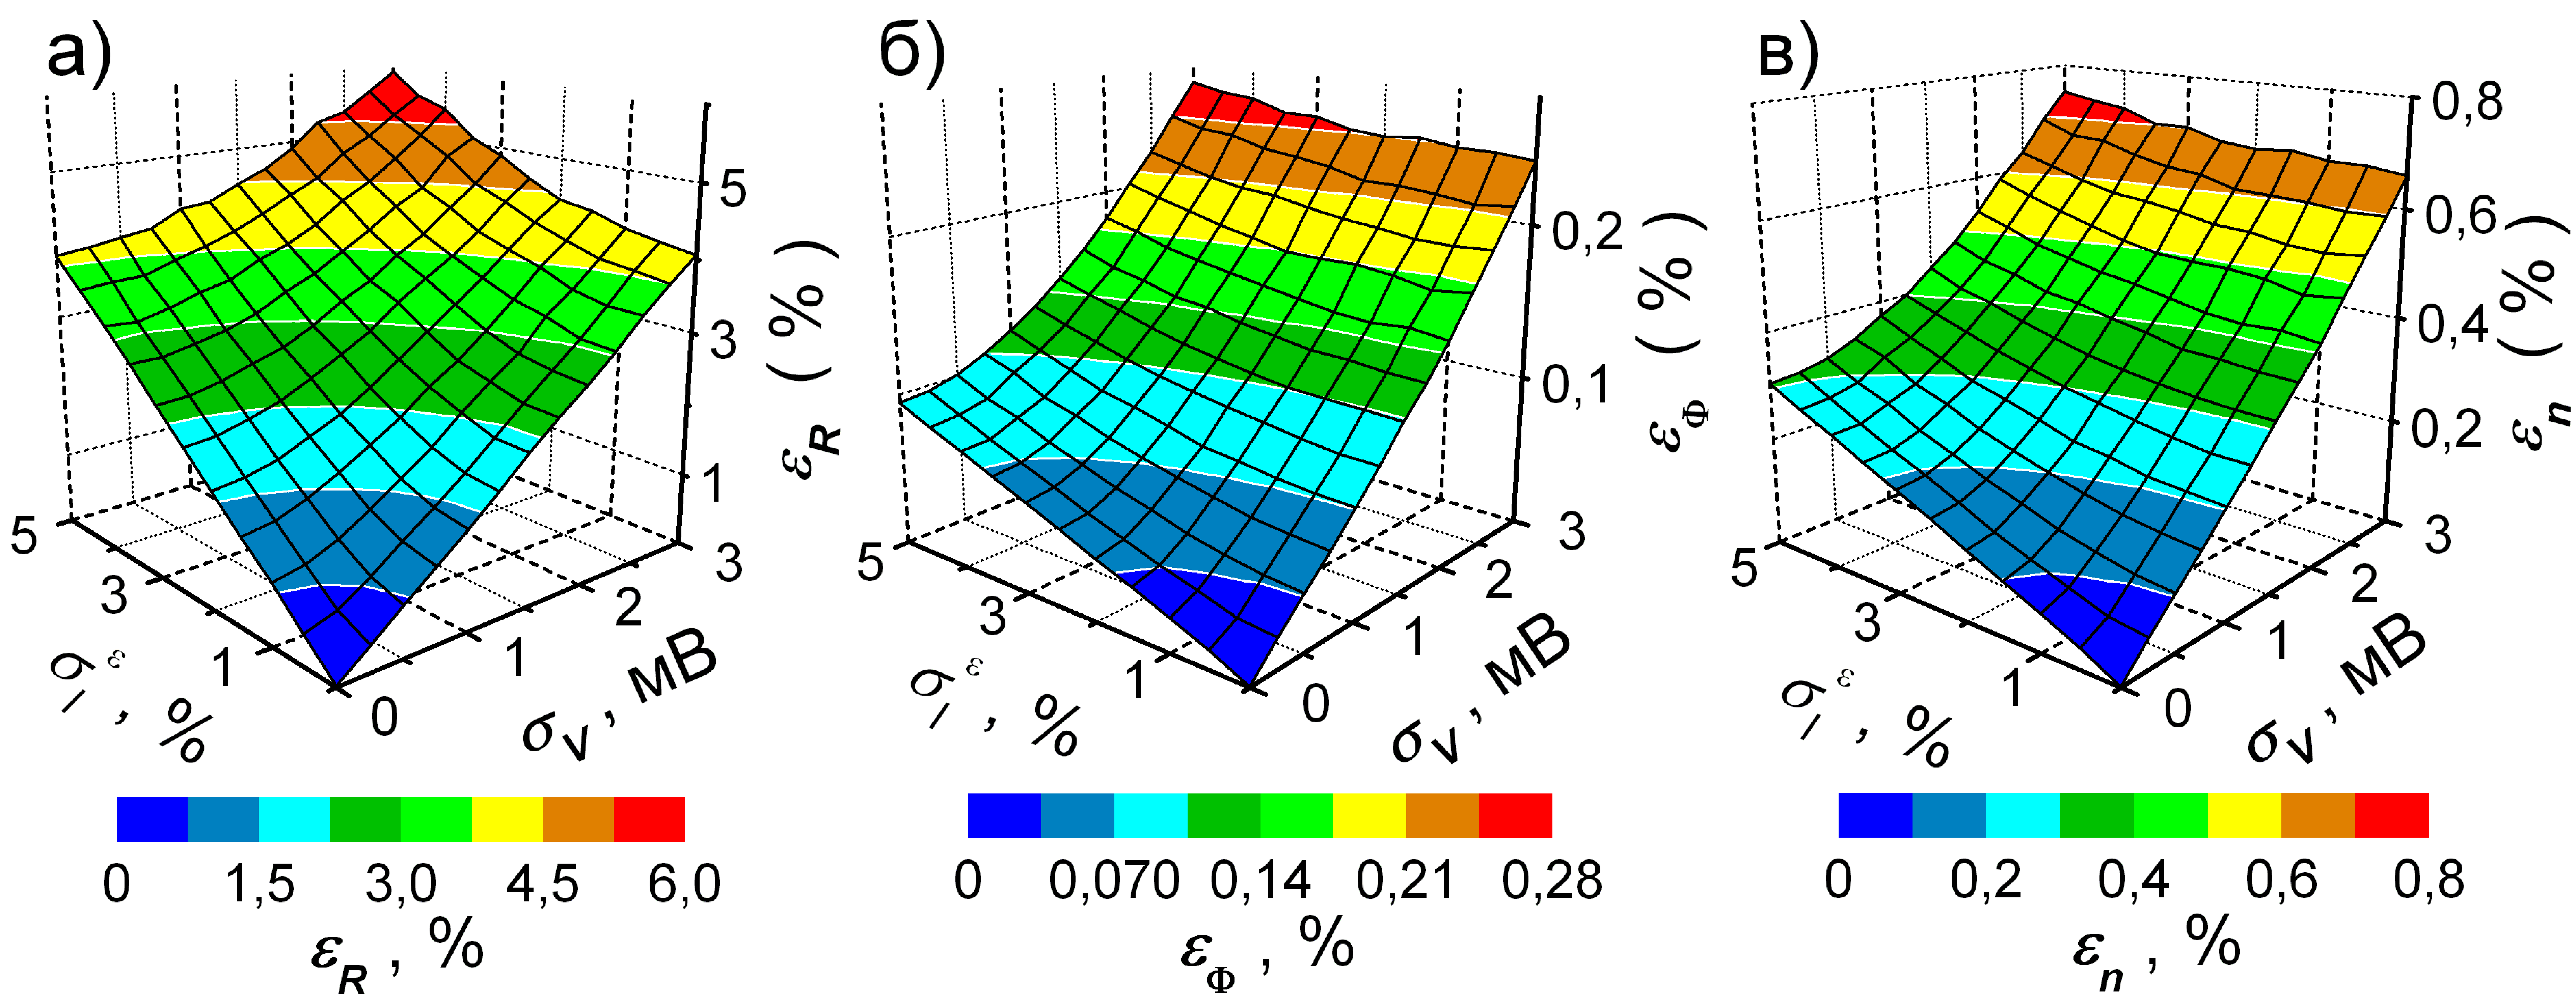
\includegraphics[width=1\textwidth]{figErr}%
\caption{\label{figErr}
Залежності похибок визначення $R_s$ (a), $\Phi_b$ (б) та $n_\mathrm{id}$ (в) при використанні методу Gromov  від похибок вимірювання сили струму та напруги
}
\end{figure}


\subsection{Визначення параметрів реальних структур метал---напівпровідник}

Температурні залежності параметрів, отриманих із експериментальних ВАХ наведені на рис.~\ref{figPract}.
Зауважимо, що в цьому випадку при застосуванні метода Bohlin використані значення $\gamma_1=1,6$ та $\gamma_2=1,8$ замість  $\gamma_1=1,6$ та $\gamma_2=3,5$, для яких, як показано в розділі~\ref{AnMethod}, очікується менше значення похибки.
Це пов'язано з тим, що для діапазону сил струму, у якому були отримані експериментальні дані, відсутній мінімум функції Норда з $\gamma_N=3.5$.



\begin{figure}
\center
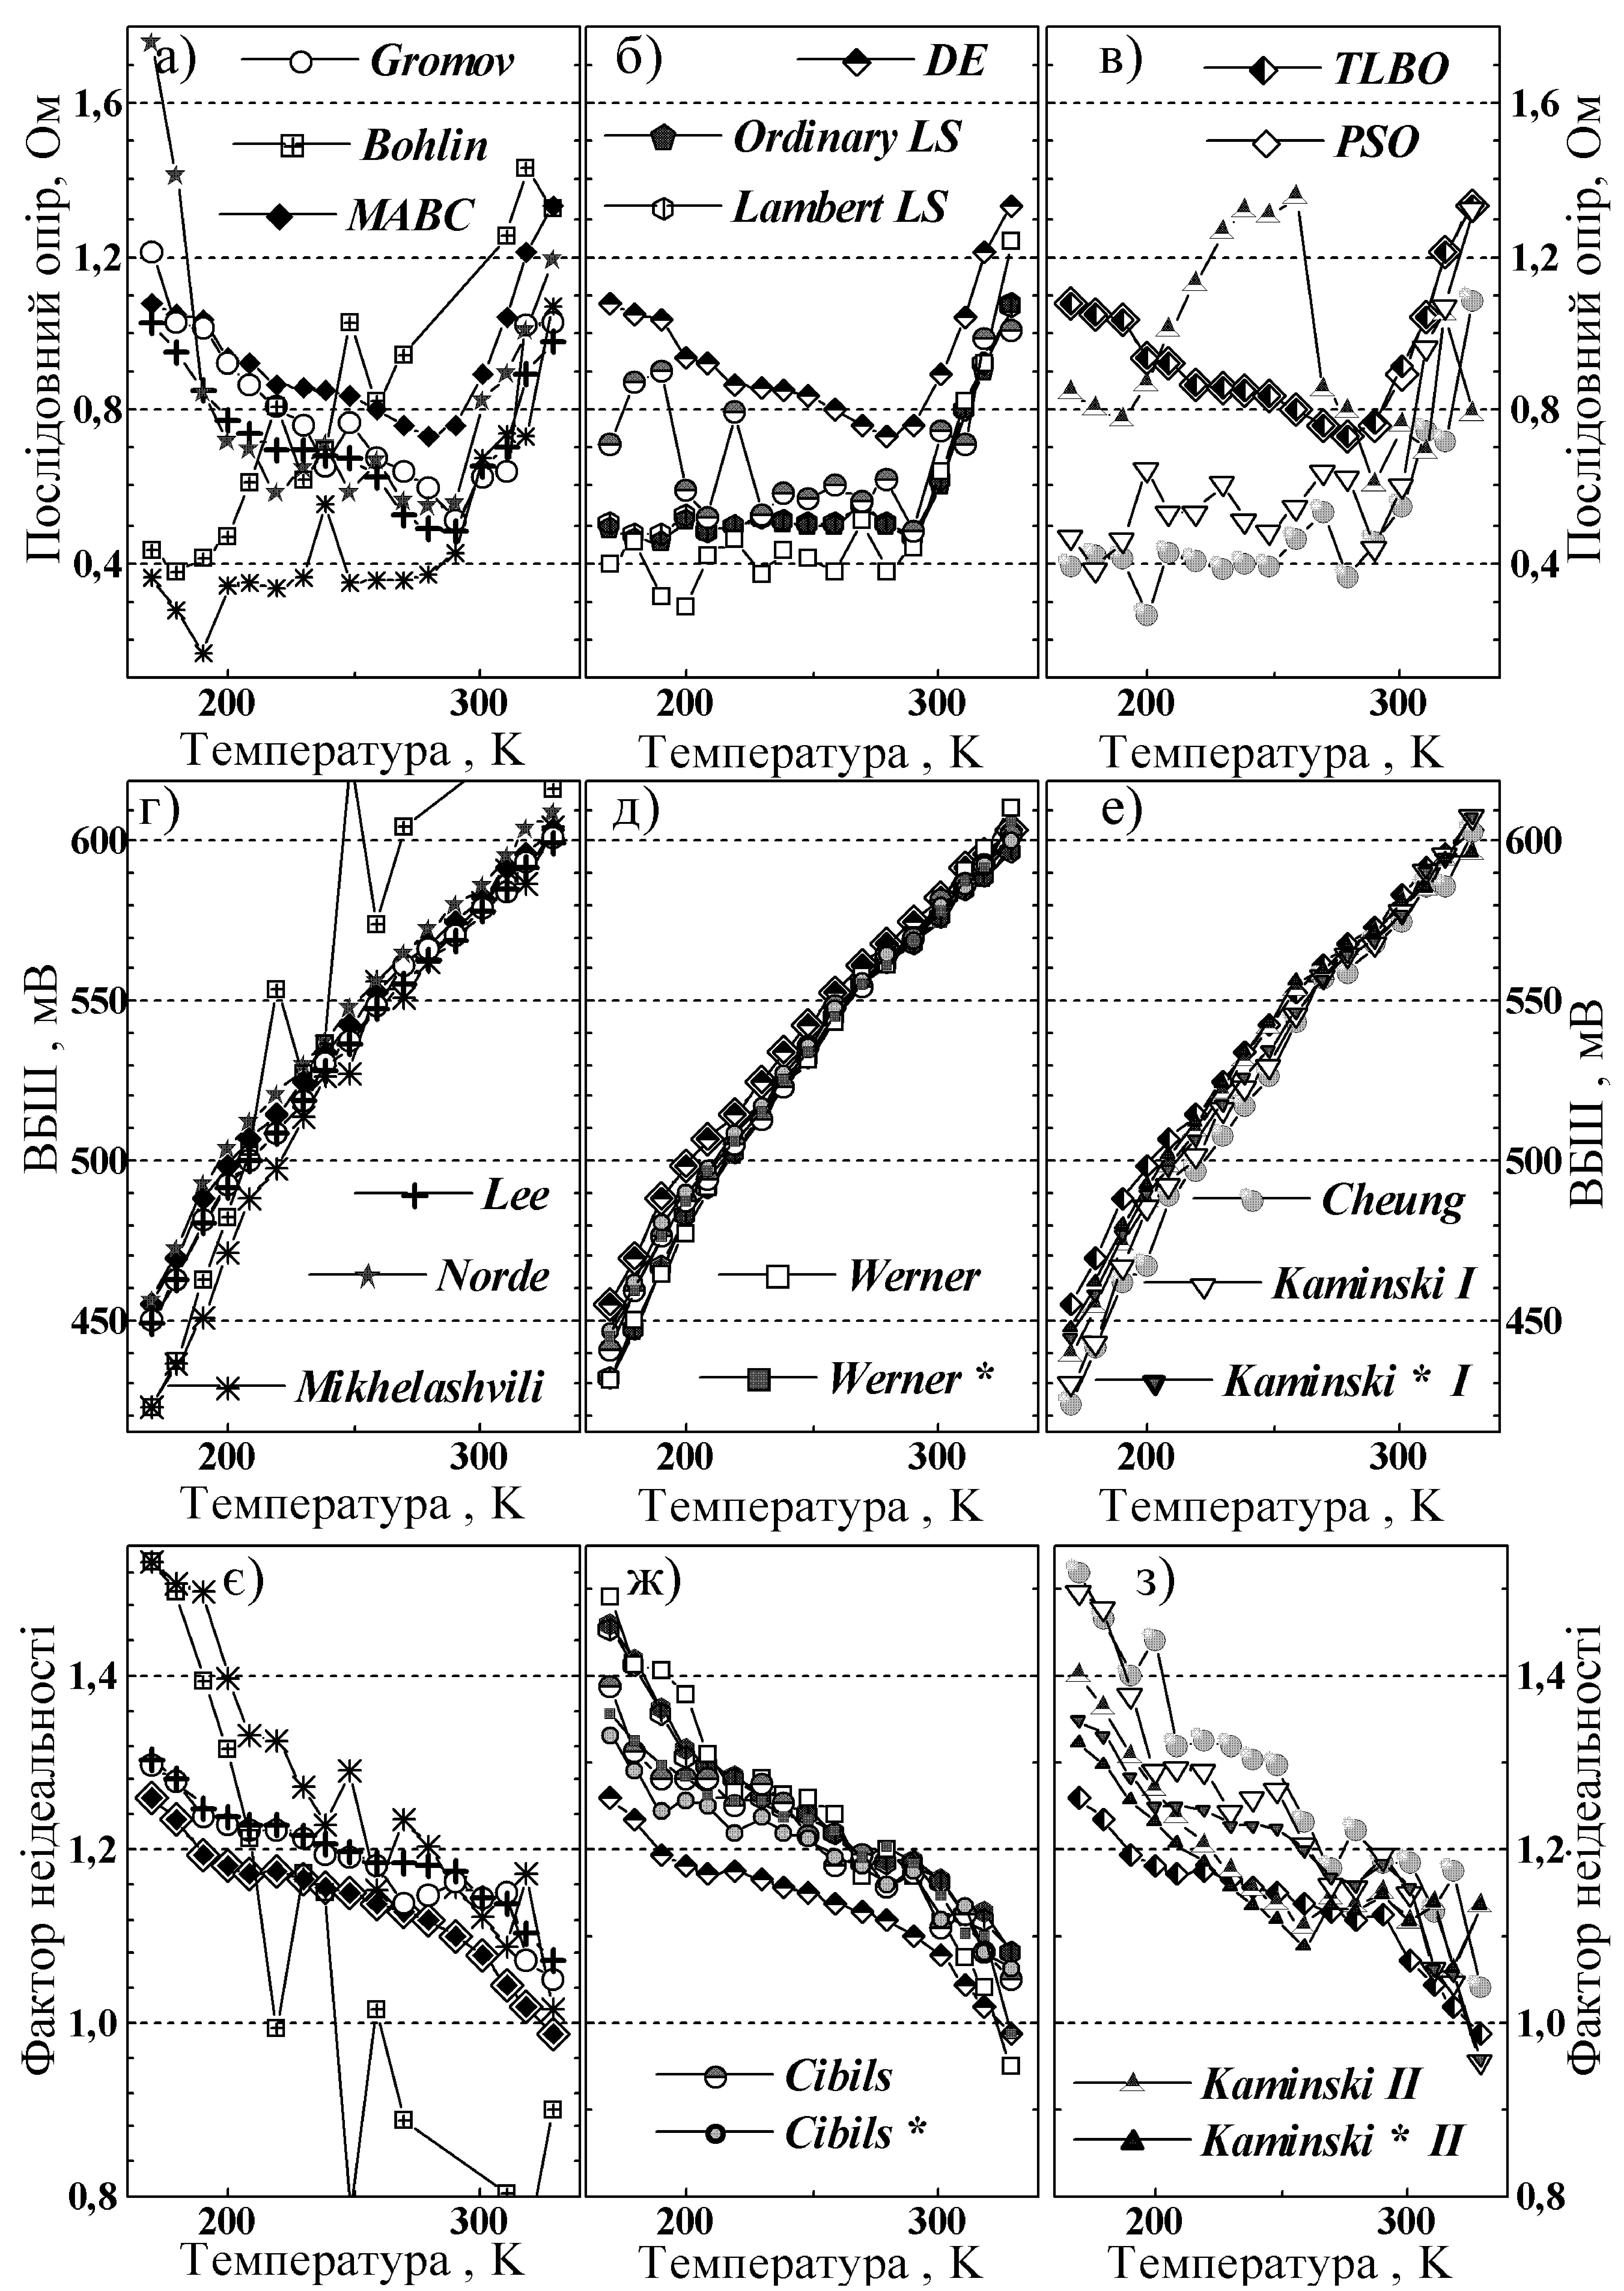
\includegraphics[width=0.8\textwidth]{figPract}%
\caption{\label{figPract}
Температурні залежності послідовного опору (а --- в), ВБШ (г --- е) та фактора неідеальності (є --- з) при
застосуванні різних методів до експериментальних ВАХ
}
\end{figure}

Виявлена температурна залежність висоти бар'єру, які відрізняється від виразу (\ref{eqFbT}), що використовувався при синтезі ВАХ, може бути пов'язана з неоднорідністю контакту МН \cite{Tung:MSE,Olikh:2013IEEE}.
Зростання послідовного опору при високих температурах в літературі \cite{Rs:Dokme} пов'язується з тим, що за цих умов визначальним для $R_s$ буде контактний опір, а не опір об'єму напівпровідника.

Зупинимось на отриманих температурних залежностях послідовного опору.
Використання ЕА, методів Gromov та Lee дозволяє виявити немонотонну температурну залежність $R_s$, причому абсолютні значення опору, отримані за допомогою різних методів, дещо відрізняються.
Взявши до уваги невелике значення послідовного опору (близько 1~Ом), а також виявлене раніше значне збільшення похибок методів Gromov та Lee при малих значеннях $R_s$ та великих $I_s$ (рис.~\ref{figId},a, \ref{figR3D},a, \ref{figR3D},б та \ref{figG1003},a), можна зробити висновок, що величини, отримані при застосуванні еволюційних алгоритмів, правильніші.
З фізичного погляду, виявлена поступова зміна опору з температурою є цілком ймовірною.
При застосуванні числових методів отримана залежність $R_s$ від $T$ також є досить гладкою, проте її поведінка відрізняється від результатів ЕА при низьких температурах (рис.~\ref{figPract},б).
Водночас, зашумленість температурних залежностей має свідчити про наявність помилок або під час вимірювань ВАХ, або під час визначення параметрів, а саме такі залежності виникають при застосуванні інших методів.

Подібні особливості характерні і для визначених залежностей ВБШ та фактора неідеальності.
Розкид значень $\Phi_b$ суттєво менший ніж для $n_\mathrm{id}$, що корелює з меншою величиною похибки визначення ВБШ (рис.~\ref{figG1003} -- \ref{figErr}).
Найгірші результати отримані при використанні методів Bohlin, Mikhelashvili та Cheung.

Для оцінки розходжень виміряних та апроксимуючих ВАХ використане середнє значення відхилення сили струму $\Delta_I$:
 \begin{equation}
 \label{eqMCur}
 \Delta_I=\frac{1}{N_p}\sum_{i=1}^{N_p}\left|\frac{I_{calc}(V_i)-I_i}{I_i}\right|.
 \end{equation}
При обчисленні $\Delta_I$, значення $I_{calc}(V_i)$ розраховувалися з використанням виразів (\ref{eqSDIV}--\ref{eqSDIs}) та параметрів, визначених при використанні різних методів.
Результати для трьох ВАХ, виміряних при різних температурах, наведені на рис.~\ref{figPrAcc}.
Як видно, в цьому випадку еволюційні алгоритми, методи Gromov та Lee також продемонстрували свої переваги.


\begin{figure}
\center
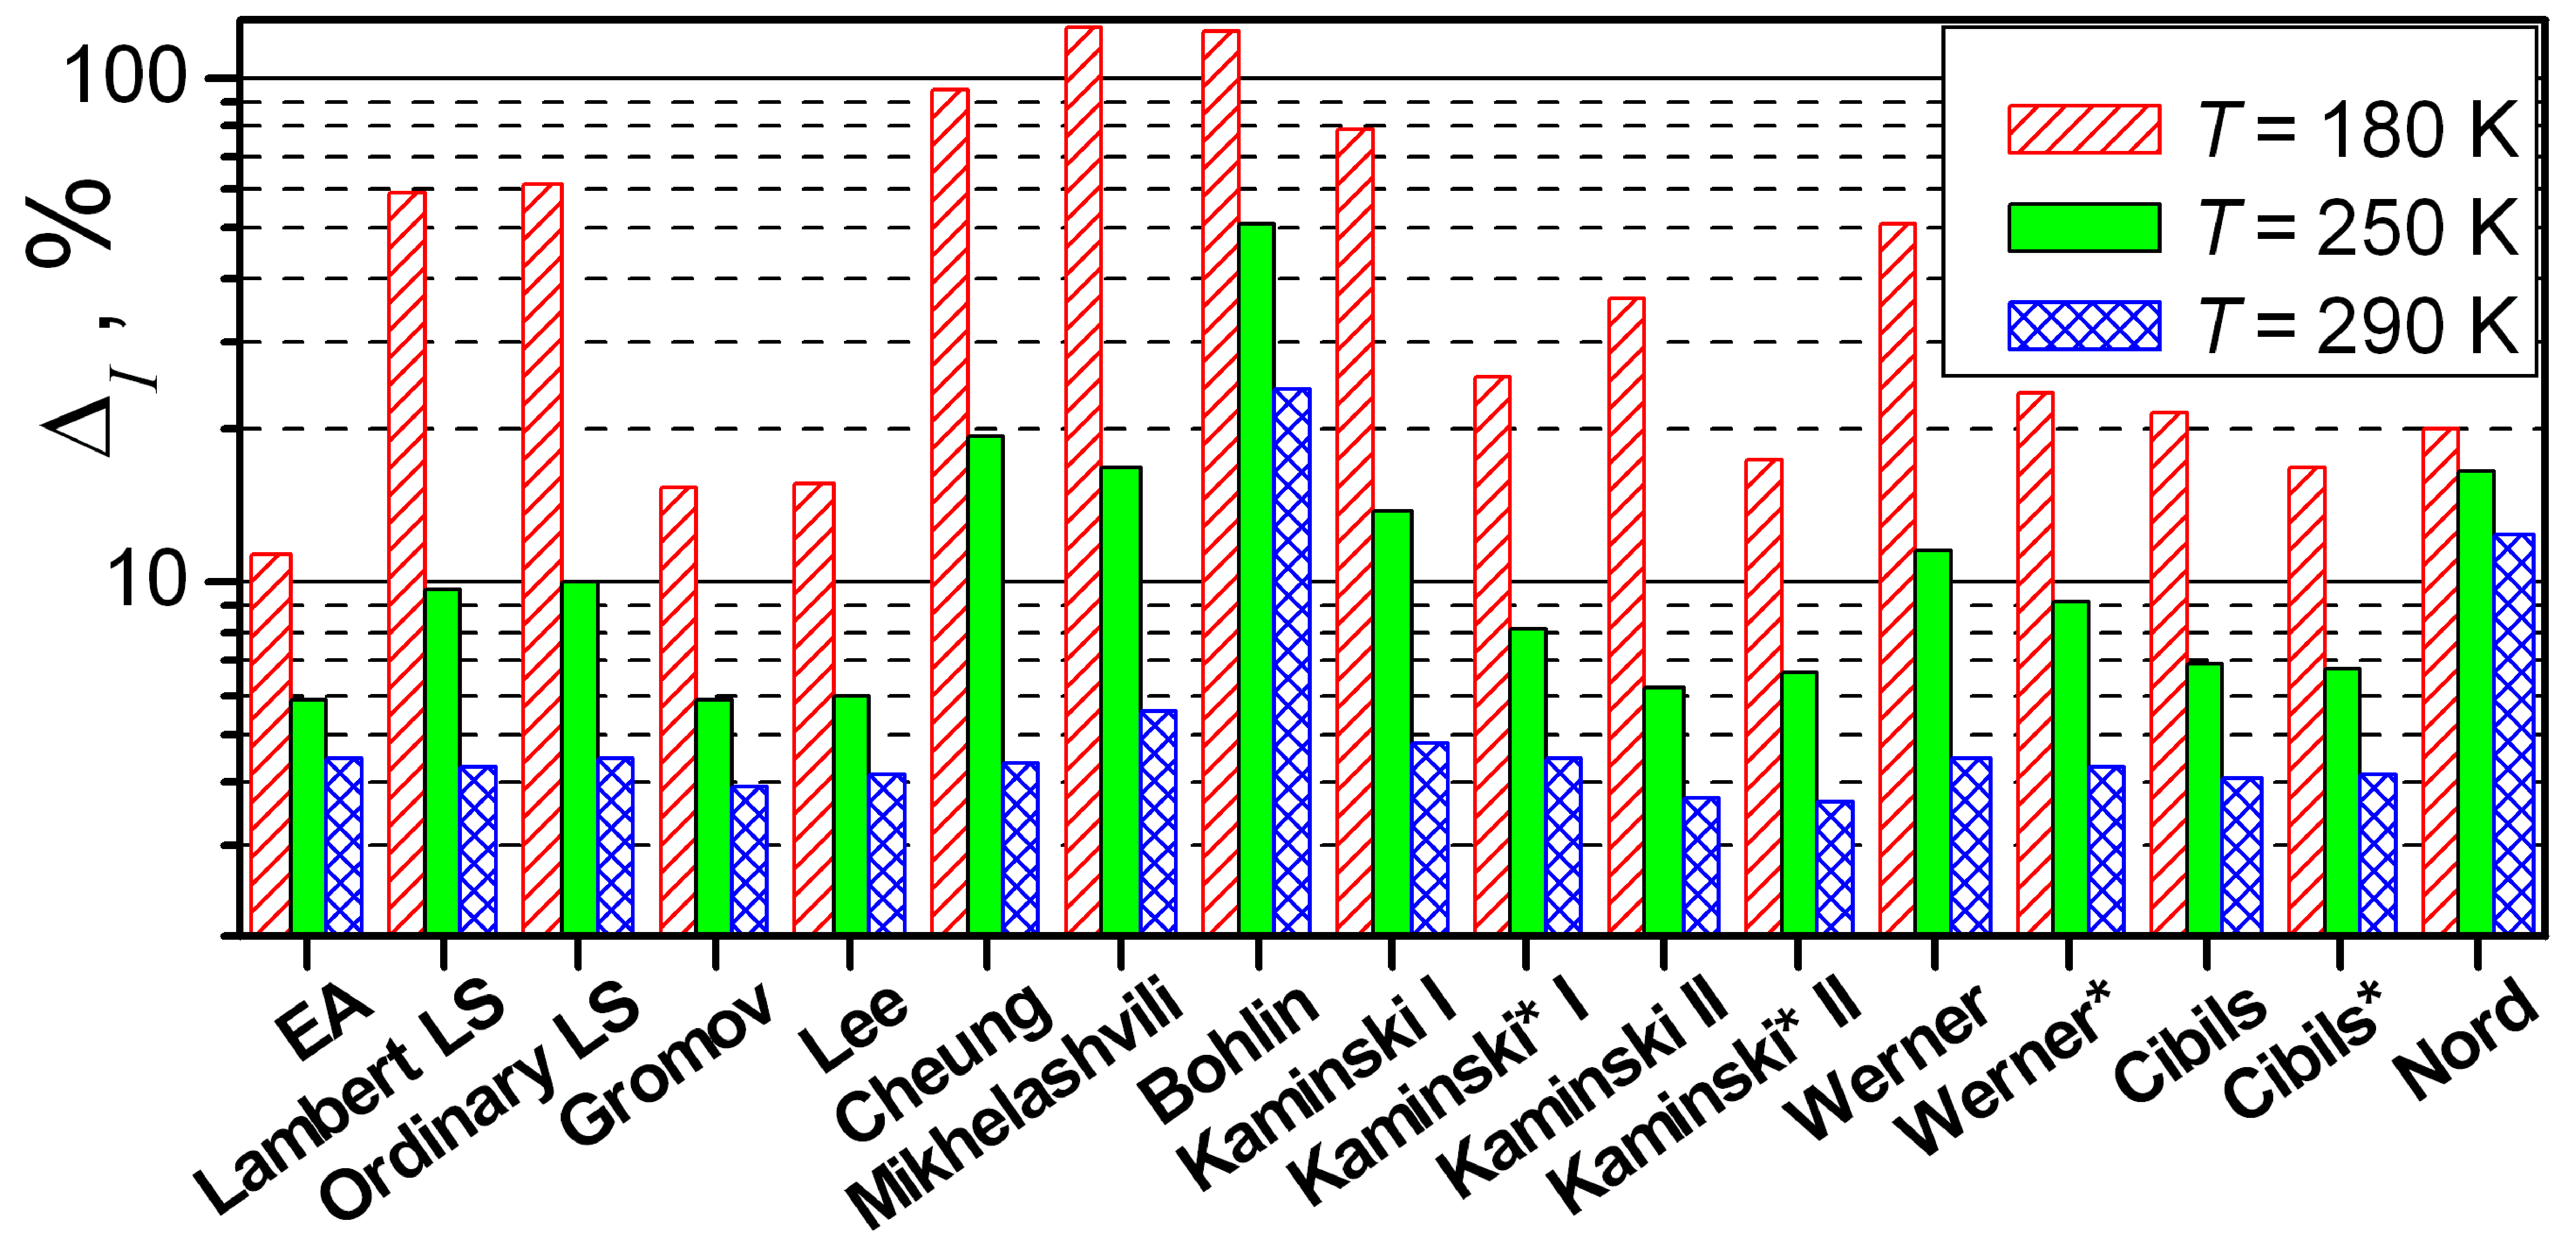
\includegraphics[width=0.8\textwidth]{figPrAcc}%
\caption{\label{figPrAcc}
Середні значення відносного відхилення розрахованих значень сили струму від експериментальних даних
}
\end{figure}

Як сказано раніше, і експериментальні ВАХ отримані для кремнієвих структур, і при синтезі даних вважалося, що ДШ створені з використанням саме цього напівпровідника.
Проте висновки щодо того, які методи є найдостовірнішими та такими, що мають перевагу, залишаються справедливими й для інших МН.
Дійсно, для діодів із іншого матеріалу можуть спостерігатися зміни  величин $\Phi_b$, $n_\mathrm{id}$, $R_s$ та співвідношень між ними.
Проте еволюційні алгоритми, методи Lee та Gromov із адаптивною процедурою довели свою перевагу для досить широкого діапазону значень параметрів.
З іншого боку, зміна матеріалу може викликати модифікацію
а)~температурної залежності точності визначення параметрів;
б)~абсолютного значення похибки.
Проте подібні зміни для конкретного напівпровідника можуть бути у першому наближені оцінені з використанням даних, наведених у табл.~\ref{tabIF}.

Необхідно підкреслити, що отримані результати будуть коректними для тих ДШ, для яких ВАХ описуються рівнянням~(\ref{eqSDIV}).
Наприклад, відхилення від цього закону характеристик реальних діодів може бути пов'язане з наявністю  опору шунтування чи неоднорідністю бар'єру \cite{Tung:MSE,OlikhJAP}.
Проте у подібних випадках застосування еволюційних алгоритмів може суттєво спростити процедуру визначення параметрів структур МН.


\section*{Висновки до розділу \ref{Ch_MSMethod}}
\addcontentsline{toc}{section}{Висновки до розділу \ref{Ch_MSMethod}}	
  \begin{enumerate}[leftmargin=0cm,itemindent=3em]
     \item Проведено порівняльний аналіз та тестування 16 основних методів визначення параметрів діодів Шотткі з вольт--амперних характеристик.
         Спираючись на результати тестування методів на експериментальних та синтезованих  ВАХ,
         запропоновано шляхи їхньої оптимізації з метою збільшення точності розрахунку.

     \item Для методу Норда проведено числовий аналіз залежності величин похибок визначення ВБШ та послідовного опору від величини параметра $\gamma_N$ на масиві синтезованих ідеальних та зашумлених ВАХ.
     Виявлено, що похибка визначення висоти бар'ру зростає зі збільшенням даного параметра, тоді як залежність похибки розрахунку послідовного опору є немонотонною функцією $\gamma_N$.
     Показано, що оптимальним значенням є $\gamma_N=1,8$.


     \item Проведено числовий аналіз залежності величин похибок визначення висоти бар'єру, фактора неідеальності та послідовного опору при використанні методу Bohlin від величин параметрів $\gamma_1$ та $\gamma_2$.
     Встановлено, що в цьому методі похибка екстрагування параметрів зростає при збільшенні величини $|\gamma_1-\gamma_2|$.
     Запропоновано оптимальні (для температурного діапазону $130\div330$~К) величини $\gamma_1=1,6$ та $\gamma_2=3,5$.



     \item Для оптимізації вибору діапазону ВАХ, який використовується для побудови допоміжних функцій при застосуванні аналітичних методів визначення параметрів структур МН, запропоновано адаптивну процедуру, що базується на аналізі відхилення між апроксимуючою та експериментальною кривими.
         На прикладі аналітичного Gromov методу показано, що дана процедура дозволяє підвищити точність визначення параметрів (приблизно на порядок при кімнатних температурах у випадку низького рівня похибок вимірювання) і не викликає критичного збільшення часу, необхідного для розрахунків.

     \item Запропоновано модифікацію методу Mikhelashvili, яка дозволяє застосовувати його в автоматичному режимі до множини ВАХ.
     Вона полягає у послідовному використанні медіанного фільтру та процедури згладжування функції $\alpha(V)=d(\ln I)/d(\ln V)$ перед визначенням положення її максимуму.
     Показано доцільність застосування запропонованої процедури при опрацюванні реальних ВАХ для підвищення точності методу, що пов'язано з можливістю визначення саме глобального екстремума.

    \item Здійснена програмна реалізація еволюційних алгоритмів  диференційної еволюції, оптимізації зграї частинок,
модифікованої штучної бджолиної сім'ї та оптимізованого викладання та навчання при вирішенні задачі визначення параметрів структур МН.
Запропоновано та показано ефективність застосування цільової функції у вигляді суми квадратів відносних похибок апроксимації кожної з точок ВАХ.
Проведено визначення необхідної кількості поколінь для збіжності кожного з алгоритмів.

   \item Показано, що серед всіх тестованих методів, найпридатнішими з погляду точності визначення параметрів є еволюційні алгоритми (особливо MABC завдяки найменшому часу розрахунку), метод Gromov із адаптивною процедурою та метод Lee, причому ЕА дозволяють отримати найкоректніші результати при малих (декілька Ом) значеннях послідовного опору або великих значеннях струму насичення (високих температурах).
    Показано, що використання функції Ламберта при числовому визначенні параметрів ДШ дозволяє зменшити похибки визначення та вплив на них інших факторів; з іншого боку, час відповідних розрахунків зростає.
    Проаналізовано залежності точностей визначення послідовного опору, висоти бар'єру Шотткі та фактора неідельності від величин параметрів та рівня випадкових помилок при вимірюванні ВАХ.

  \end{enumerate}

Предсталені в даному розділі результати огляду, тестування та порівняльного аналізу методів визначення параметрів діодів Шотткі будуть корисними для подальших дослідження та розробки
МН пристроїв.

Основні результати даного розділу представлені та використані в роботах \cite{Olikh:Rev,6CPFCS,OlikhJAP,Olikh:Ultras2016,Olikh2016JSem}.


\chapter{\MakeUppercase{Ефекти впливу} $\gamma$--\MakeUppercase{опромінення та ультразвукового навантаження при кімнатних температурах
на структури} Al---$n$--$n^+$--Si \MakeUppercase{з контактом Шотткі}\label{Ch_GammaSD}}

Як відомо, структури метал---напівпровідник  є основою для створення різноманітних польових транзисторів, детекторів високочастотного
випромінення, сонячних елементів тощо;
діоди з контактом Шотткі широко використовуються під час виробництва високошвидкісних логічних, інтегральних та оптоелектронних елементів
і тому інтерес до подібних структур з боку науковців є цілком зрозумілим.
Одним із основних підходів для опису струму через контакт МН є теорія термоелектронної емісії (ТЕ),
згідно з якою \cite{Colinge,Sze2012,Rhoderick1988,StrihaBook} ВАХ має описуватися виразами (\ref{eqSDIV})--(\ref{eqSDIs}),
причому фактор неідеальності має бути рівний одиниці, послідовний опір нульовим,
а ВБШ визначається різницею між роботою виходу електрону з металу та енергією електронної спорідненості в напівпровіднику \cite{Colinge}.
Проте для реальних структур МН ці вирази нерідко є занадто спрощеними, оскільки
слід враховувати дію сил зображення, наявність проміжного діелектричного прошарку та електронних станів на межі розділу,
неоднорідність контакту, падіння прикладеної напруги не лише в області збідненого шару напівпровідника тощо.
Як наслідок, зокрема, величини $\Phi_b$ та $n_\mathrm{id}$ стають залежними від стану контакту та температури.
Окрім ТЕ, вірогідними причинами перенесення заряду в структурах МН є генераційно-рекомбінаційні процеси в області переходу,
різноманітні процеси витоку струму, тунелювання, термопольова емісія,
причому в двох останніх випадках суттєву роль можуть відігравати локальні енергетичні рівні \cite{Rhoderick1988,Evstropov,VRH:Lee,Sathaiya,Arslan,Donoval2010,Huang}.
Як наслідок, сумарний струм часто розглядають у вигляді суми декількох доданків,
кожний з яких зумовлений окремим механізмом перенесення заряду і може домінувати у своєму температурному чи польовому діапазоні \cite{Arslan,Donoval2010,Huang,GELCZUK2014}.
Зауважимо, що через суттєве різноманіття факторів впливу, задача про передбачення за певних
(у тому числі й температурних) умов механізму перенесення струму в структурах із бар'єром Шотткі є складною і такою, що не має загального вирішення.

З іншого боку, технічний розвиток передбачає розширення вимог до умов, у яких мають функціонувати напівпровідникові прилади.
Наприклад, подібні системи нерідко повинні працювати за умов різноманітного опромінення, наприклад, у космосі чи на атомних електростанціях.
Електрофізичні властивості структур МН дуже чутливі до стану межі розділу і будь--які
зовнішні фактори, що модифікують інтерфейс, суттєво впливають також і на властивості ДШ.
Радіація є одним із таких факторів і тому вивчення впливу опромінення на характеристики МН структур є дуже важливим не лише завдяки
тому, що подібні дослідження дозволяють краще зрозуміти механізми та наслідки взаємодії налітаючих частинок із твердим тілом,
але й через своє широке практичне застосування.
Звичайно, на подібні дослідження звертається чимала увага  --- див., наприклад,
\cite{Kumar1, Rao, Kumar2, Sharma, Ohyama, Tataroglu,Tascioglu2010old,Tataroglu:2007NIMA,Tataroglu3,Karatas:2006NIMA,Umana,Kinoshita,Vorobets,Pattabi,Kovalyuk,Verma,Abdolahpour}.
Проте результати, отримані різними дослідниками, нерідко не повністю збігаються.
Наприклад, виявлено, що ВБШ внаслідок  опромінення може як зменшуватися \cite{Kumar1, Rao, Kumar2, Sharma, Ohyama,Tataroglu3},
так і збільшуватися \cite{Tataroglu,Tascioglu2010old,Tataroglu:2007NIMA}.
Крім того, спостерігалися також ефекти немонотонної зміни висоти бар'єру при збільшенні поглинутої дози \cite{Karatas:2006NIMA,Umana,Kinoshita,Vorobets, Pattabi, Kovalyuk,Verma}, причому повідомляється як про немонотонність типу <<спад--зростання>> так і <<зростання--спад>>.
Причини подібного різноманіття характеру радiацiйноiндукованих змін висоти
бар'єру досі залишалися невідомими,
а відтак, питання вимагає подальших досліджень.


Нарешті, незважаючи на достатньо широке експериментальне підтвердження можливості ефективного використання УЗ для впливу на властивості різноманітних напівпровідників та
пристроїв на їхній основі
\cite{Bahar2003,ZobovFTP2008,Parchinskii2006r,Roman:2007APL,Roman:2010JAP,Zaver2005,Davletova2008,Teterkin2009r,Tagaev,Pashaev2012r,YOlikhTPL2011r,Zaveryukhin2002:2},
роботи, присвячені акустодинамічним явищам у ДШ, практично відсутні.
Отже, основна мета досліджень, результати яких розглянуті у даному розділі, полягала у наступному:
\begin{itemize}[leftmargin=0cm,itemindent=1em]
  \item з'ясування механізмів перенесення заряду  при прямому та
    зворотному зміщеннях у структурах Al---$n$--$n^+$--Si у діапазоні температур 130$\div$330~К;
  \item вияснення причин немонотонних змін висоти бар'єру кремнієвих ДШ при $\gamma$--опромінення;
  \item вивчення впливу УЗН при кімнатній температурі на процеси перенесення заряду в МН--структурах на основі Si.
\end{itemize}



\section{Загальна характеристика структур Al---$n$--$n^+$--Si\label{MSSi}}

\begin{figure}[b]
\center
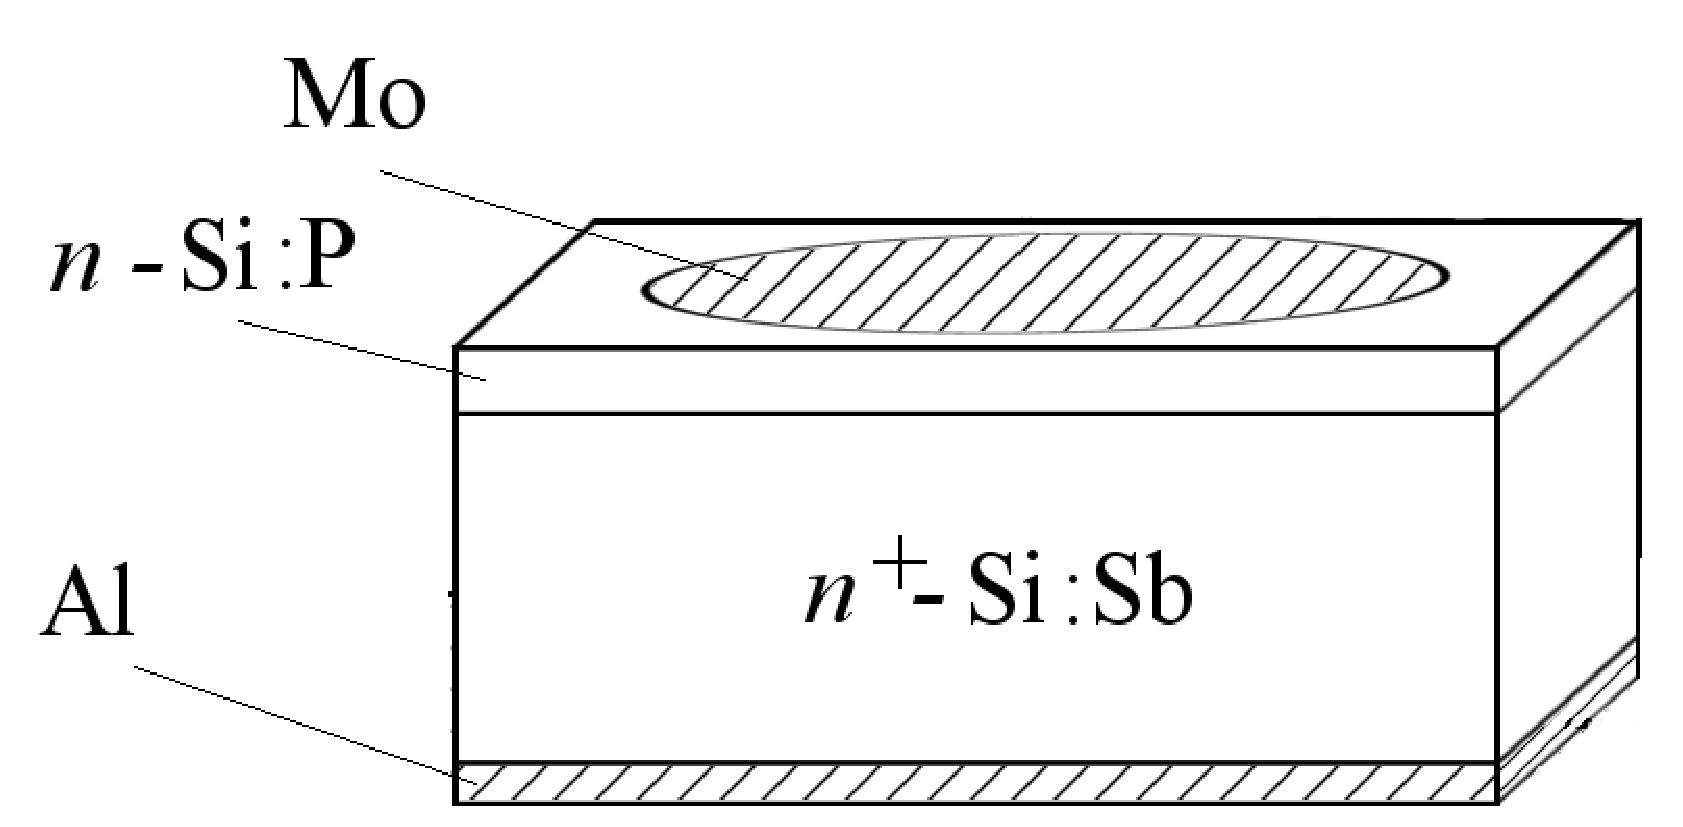
\includegraphics[width=0.4\textwidth]{MSSi}%
\caption{\label{figMSSi}
Структура зразків SSDA}
\end{figure}

%Для досліджень використовувалися діоди Шотткі з наступною структурою:
%на підкладці $n^+$-Si:Sb (KЭС~0.01, товщина 250~мкм) знаходиться епітаксійний шар $n$-Si:P (товщина 0.2~мкм);
%на поверхні епі-шару створено контакт  Шотки діаметром 2 мм шляхом нанесення шару молібдену;
%на протилежному боці підкладки --- омічний контакт.


У цьому розділі розглянуті результати дослідження діодів Шотткі Al---$n$--$n^+$--Si,
виготовлених за стандартною технологією \cite{Vorobets:FM2003,StrihaBook1987} на пластинах кремнію КЭФ1 товщиною $250$~мкм
з орієнтацією (111).
Пластини хімічно очищалися, із неробочої поверхні
повністю видалявся попередньо сформований шар SiO$_2$ для легування фосфором.
На робочій поверхні хімічним травленням створювалися вікна в SiO$_2$ і проводилося очищення
за допомогою іонного пучка.
Потім на робочу поверхню напилювалася алюмінієва плівка і проводився процес фотолітографії.
Після цього на протилежну поверхню наносився шар алюмінію товщиною близько 1~мкм і проводився відпал
у інертній атмосфері.
Внаслідок термічної обробки утворювалася структура з випрямляючим контактом на робочій поверхні і омічним на протилежній.
Схематичне зображення структури діодів Шотткі Al---$n$--$n^+$--Si наведено на рис.~\ref{figMSSi},
надалі вони позначаються SSDA.

Діаметр контакту Шотткі складав 2 мм (площа ДШ $A=3,14\cdot10^{-6}$~м$^2$).
Для контролю рівня легування приповерхневого шару проведені
вимірювання вольт--фарадних характеристик (ВФХ) досліджуваних структур при кімнатній температурі ($T = 295$~К).
Приклад отриманої залежності наведено на рис.~\ref{figCV}.
Лінійність залежності $C^{-2}$ від $V$
(де $C$ --- ємність діода Шотткі)
у широкому діапазоні зворотних напруг свідчить про рівномірність легування.
Виявлено, що концентрація носіїв заряду в приповерхневому шарі $N_d\approx1,2\cdot10^{23}$~м$^{-3}$.


\begin{figure}
\center
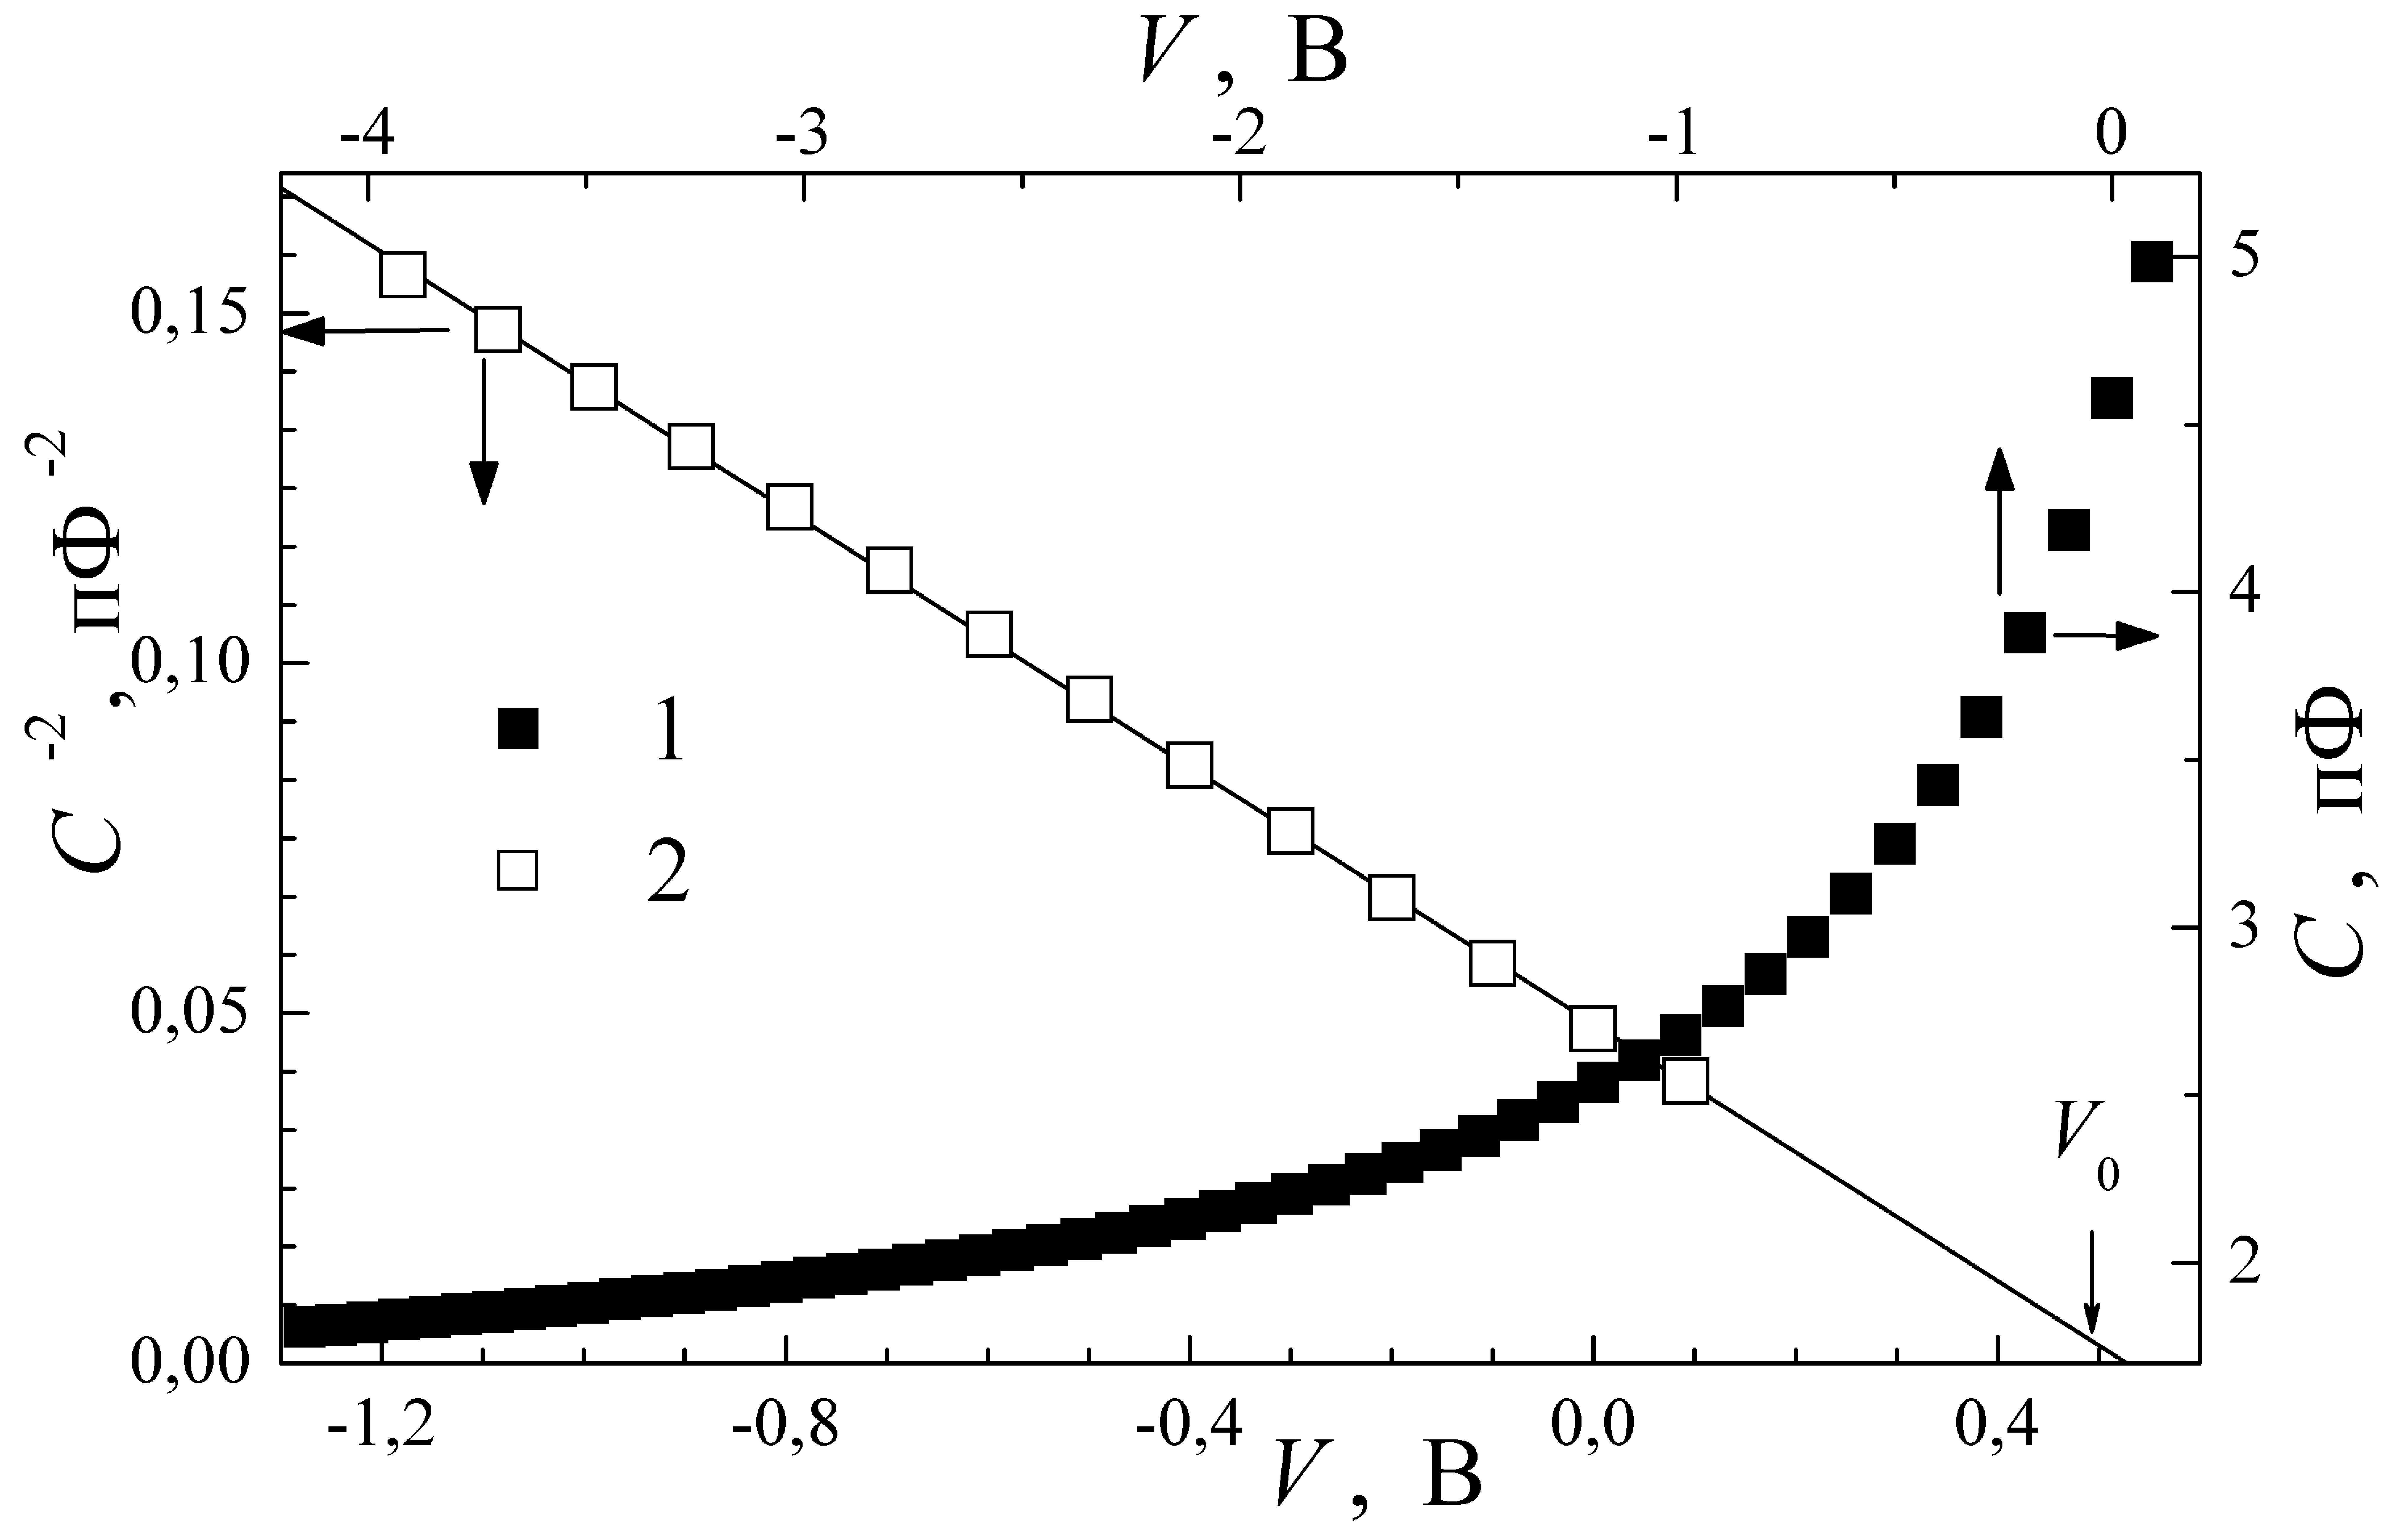
\includegraphics[width=0.7\textwidth]{figCV}
\caption{\label{figCV}
Залежність ємності Al---$n$--$n^+$--Si діодів Шотткі $C$ (крива 1) та величини $C^{-2}$ (2) від прикладеної напруги.
$T=295$~К.
Точки --- експеримент, пряма --- лінійна апроксимація 2.
}%
\end{figure}







%В дисертації представлені результати, отримані з використанням кремнієвих ДШ двох типів,
%які ідентичних за структурою, проте відрізняються концентраціями концентраціями носіїв заряду в епітаксійному шарі $N_d$ та
%підкладці $N_s$, а також площею випрямляючого контакту $A$.
%Для контролю рівня легування були виконані вимірювання вольт--фарадних характеристик (ВФХ) досліджуваних структур при кімнатній температурі ($T = 295$~К).
%Параметри структур, а також їх позначення наведені в Таблиці~\ref{tabMSSi}.



Вимірювання ВАХ даних структур проводилося у діапазоні зміни постійного струму $(10^{-9}\div10^{-2})$~А при
прямому та зворотному зміщеннях із кроком по напрузі 0.01~В у інтервалі температур $(130\div330)$~К.


\section{Особливості перенесення заряду в структурах Al---$n$--$n^+$--Si з бар'єром Шотткі\label{MSSi_Non}}
\subsection{Пряме зміщення\label{sbMSSi_NonF}}

%\subsubsection{Особливості аналізу експериментально виміряних ВАХ}

Приклади виміряних прямих ВАХ при різних температурах наведено на рис.~\ref{figIV_SDA}.
Видно, що при температурі більше 250~К прямі ВАХ в напівлогарифмічному масштабі є практично лінійними в інтервалі зміни струму близько трьох порядків.
Водночас, при $T<210$~K загальний струм можна розділити на дві складові, причому для ВАХ, пов'язаної зі струмом,
який домінує при малих зміщеннях, суттєвим є вплив послідовного опору.
Про це свідчить відхилення від лінійності наведених кривих при при $7\cdot10^{-8}\mbox{A}<I<5\cdot10^{-7}\mbox{A}$.

У літературі \cite{Rhoderick1988,Gromov,Sze2012} показано, що в реальних структурах МН для опису залежності струму від прикладеної прямої напруги
навіть при врахуванні лише термоемісійних процесів замість виразу~(\ref{eqSDIV}) доцільно використовувати наступний
\begin{equation*}
I=I_s\exp\left[\frac{q(V-IR_S)}{n_\mathrm{id}kT}\right]\cdot
\left\{1-\exp\left[-\frac{q(V-IR_S)}{kT}\right]\right\}.
\end{equation*}
У зв'язку з цим для опису прямих гілок ВАХ використано вираз
\[
I=I_1+I_2=I_{s1}\exp{\left(\frac{qV}{n_{\mathrm{id},1}kT}\right)}\cdot
\left[1-\exp{\left(-\frac{qV}{kT}\right)}\right]+\]
\begin{equation} \label{eqSDA_IV}
+I_{s2}\exp\left[\frac{q(V-IR_S)}{n_{\mathrm{id},2}kT}\right]\cdot
\left\{1-\exp\left[-\frac{q(V-IR_S)}{kT}\right]\right\},
\end{equation}
де перший доданок $I_1$ є основним при $I>10^{-5}$~A, а другий $I_2$ --- при $I<5\cdot10^{-7}$~A.
Використання двох доданків для опису ВАХ бар'єрних структур широко використовується
в літературі --- див., наприклад, \cite{Arslan,Donoval2010,Huang,GELCZUK2014}.
Зауважимо, що іншим поширеним методом врахування наявності особливостей на ВАХ при малих зміщеннях є введення опору шунтування, а не доданку $I_2$.
Проте у цьому випадку такий підхід не є виправданим, оскільки навіть при найменший зміщеннях пряма ділянка ВАХ не є лінійною --- див. вставку на рис.~\ref{figIV_SDA}.

\begin{figure}
\center
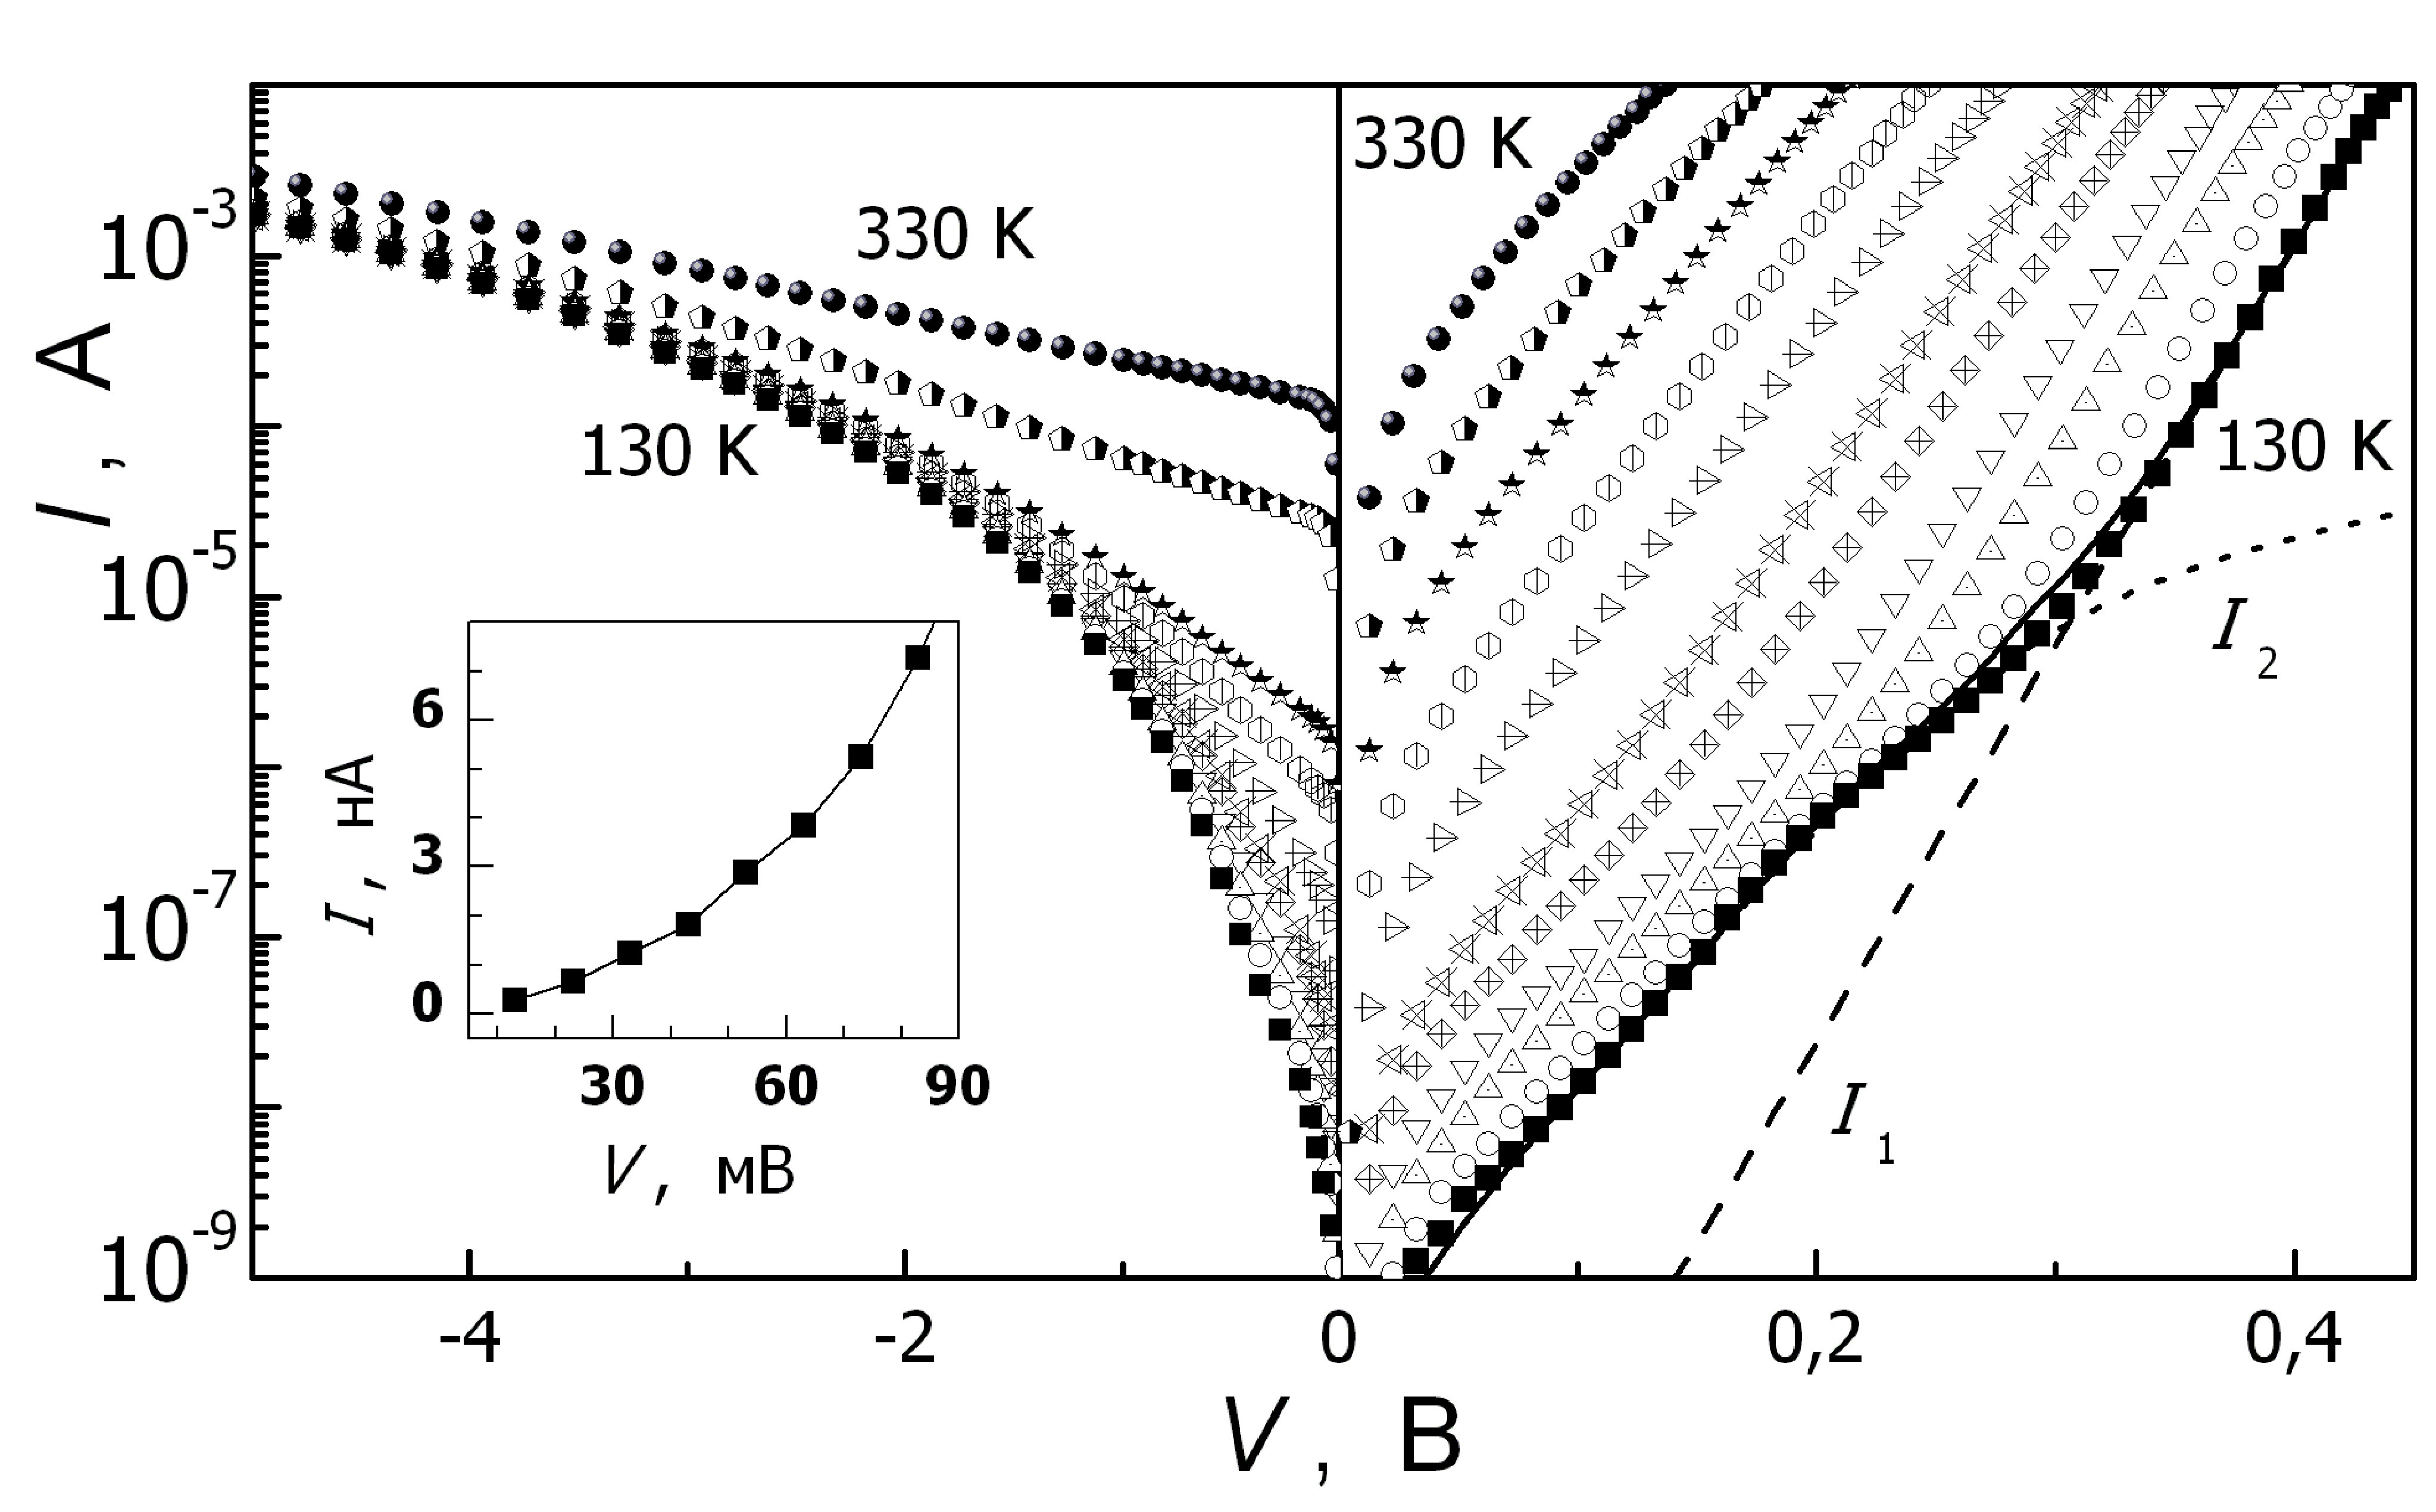
\includegraphics[width=0.8\textwidth]{figIV_SDA}
\caption{\label{figIV_SDA}
Прямі  ділянки ВАХ структур SSDA у інтервалі температур 130$\div$330~К.
Наведено криві, виміряні з кроком 20~К.
Лінії --- апроксимація прямої ВАХ при $T=130$~К за формулою~(\ref{eqSDA_IV}):
штрихова -- струм $I_1$, пунктирна -- $I_2$,
суцільна -- $I_1+I_2$;
параметри апроксимації $n_{\mathrm{id},1}=1,67$,
$n_{\mathrm{id},2}=2,53$,
$I_{s1}=5,0\cdot10^{-13}$~A,
$I_{s2}=3,8\cdot10^{-10}$~A, $R_{s}=4.1\cdot10^3$~Ом.
На вставці --- початкова ділянка прямої ВАХ при $T=130$~K
}%
\end{figure}

Для визначення апроксимаційних параметрів використовувалася наступна процедура.
Пряма ВАХ розбивалася на дві ділянки:
$10^{-5}\mbox{A}<I<10^{-2}\mbox{A}$ та
$10^{-9}\mbox{A}<I<10^{-7}\mbox{A}$.
Використовуючи дані першої, виконувалась побудова залежності величини $\ln{{I}/{\left[1-\exp\left(-qV/kT\right)\right]}}$ від $V$, яка надалі
апроксимувалася за методом найменших квадратів прямою,
кутовий коефіцієнт та вільний член якої пов'язані з $n_{\mathrm{id},1}$ та $I_{s1}$ відповідно.
Спираючись на дані другої ділянки ВАХ і використовуючи методи Cheung \cite{Cheung} та Gromov \cite{Gromov}, визначалась величина $R_s$.
Використання двох методів мало на меті підвищити достовірність отриманих даних і воно показало, що отримані обома шляхами значення близькі (в межах 10\%) між собою.
Після визначення $R_s$, будувалась залежність $\ln (I /\{1 - \exp[ -q (V - IR_s) / (kT ) ]\})$ від
ефективної напруги $(V-IR_s)$ і для визначення $I_{s2}$ та $n_{\mathrm{id},2}$ використовувалася процедура, аналогічна першій ділянці.

На рис.~\ref{figIV_SDA} наведено приклад апроксимації експериментальної прямої ВАХ при одній з температур за формулою \eqref{eqSDA_IV} з використанням параметрів,
отриманих із використанням описаної процедури.
Видно задовільний збіг розрахованої кривої та експериментальних точок.

У випадку, коли проходження струму через бар'єр визначається ТЕ, то висота бар'єру Шотткі при
нульовому зміщенні $\Phi_b$ пов'язана зі струмом насичення співвідношенням \cite{Rhoderick1988}:
\begin{equation}
\label{eqFb:TE}
\Phi_b=\left(\frac{kT}{q}\right)\cdot\ln\left(\frac{AA^*T^2}{I_s}\right).
\end{equation}
Отримані температурні залежності для висот бар'єрів та факторів неідеальності обох компонент струму наведено на рис.~\ref{figFbT_SDA}.

%Розглянемо спочатку особливості струму, переважаючого при високих температурах та великих зміщеннях ($I_1$).


\begin{figure}
\center
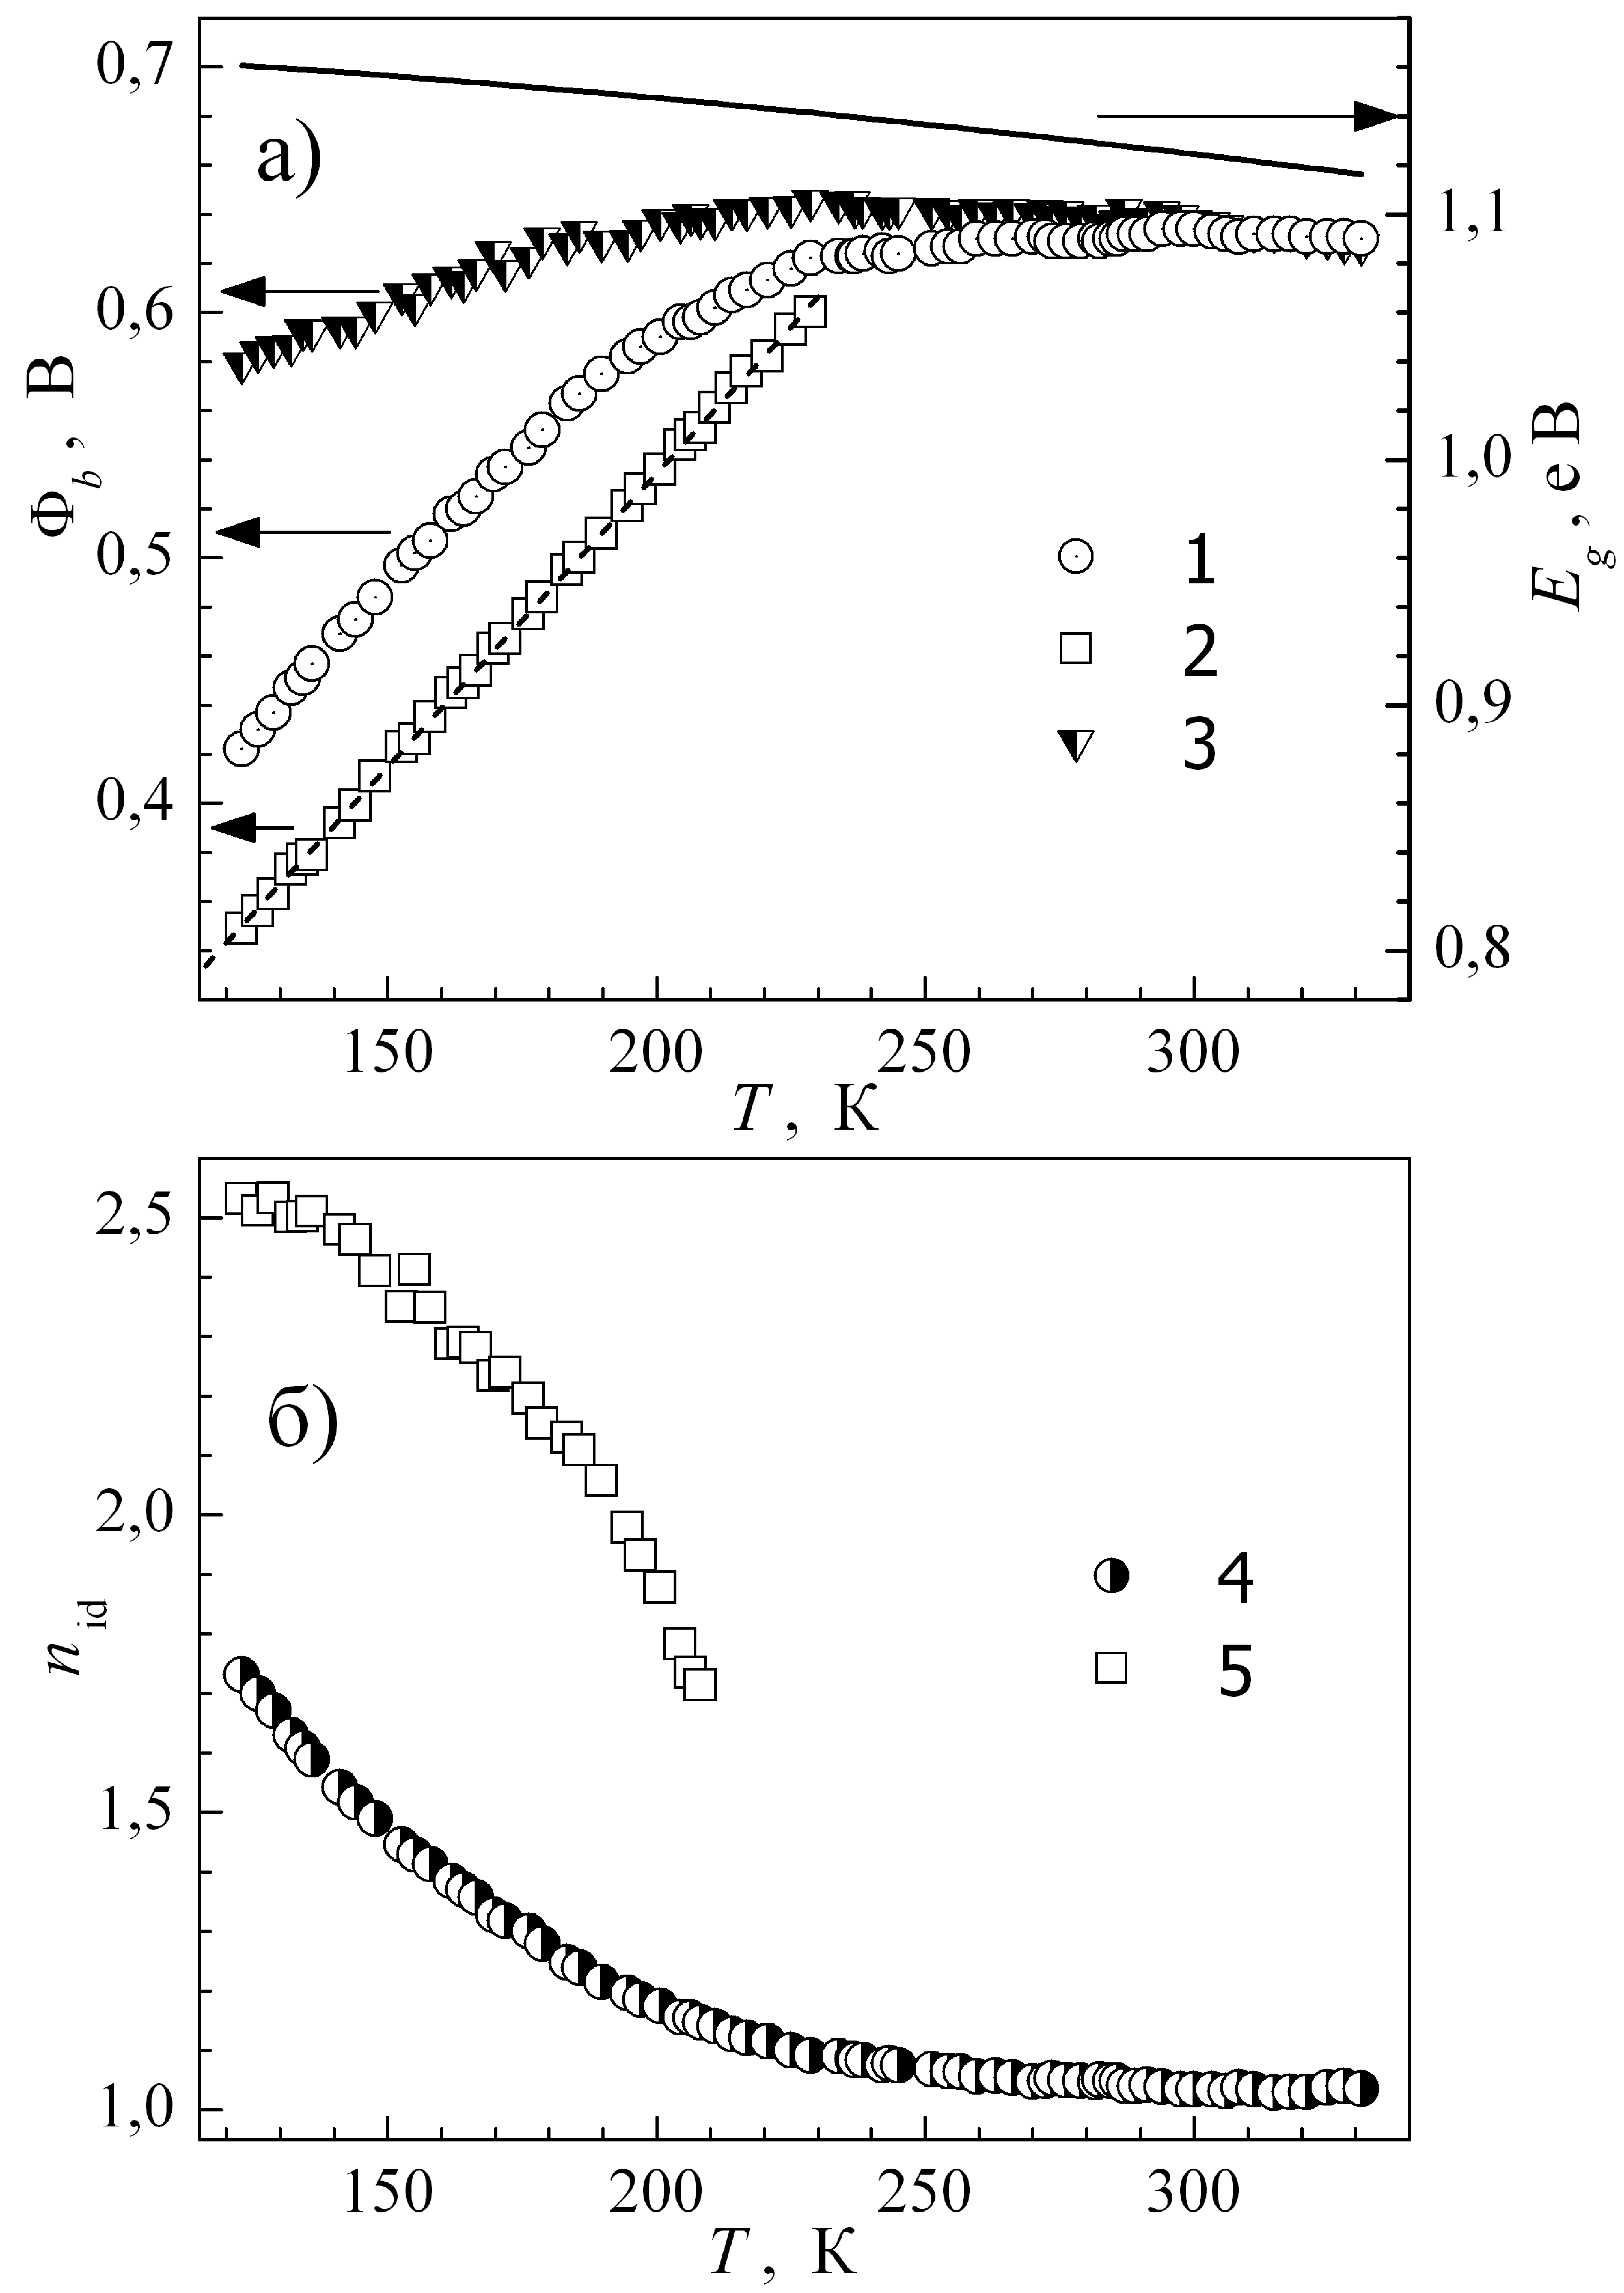
\includegraphics[width=0.95\textwidth]{figFbT_SDA}
\caption{\label{figFbT_SDA}
Температурні залежності висоти бар'єру (а) та фактора неідеальності (б) структури SSDA.
1 -- $\Phi_{b1}$,
2 -- $\Phi_{b2}$,
3 -- $\Phi_{b1}^\mathrm{eff}$ ,
4 -- $n_{\mathrm{id},1}$, 5 -- $n_{\mathrm{id},2}$.
Пунктир -- лінійна апроксимація кривої 2.
Також приведено температурну залежність ширини забороненої зони Si (а, суцільна лінія)
}%
\end{figure}

З рисунка видно, що при збільшенні температури фактор неідеальності зменшується, наближаючись
до одиниці при кімнатних температурах.
Як відомо, температурна залежність фактора неідеальності залежить від механізму перенесення заряду.
Зокрема, для ідеального випадку ТЕ очікується, що $n_{\mathrm{id}}=1$ при будь--яких температурах.
Проте для реальних контактів така рівність не спостерігається і для опису залежності $n_{\mathrm{id}}(T)$в рамках теорії ТЕ
часто використовують вираз \cite{Rhoderick1988, Sze2012}
\begin{equation}\label{eqN_T:TE}
n_{\mathrm{id}}=1+\frac{T_0}{T},
\end{equation}
де $T_0$ --- певна константа, що не залежить від температури та зміщення в широкому температурному інтервалі.

Проте залежність, подібна до зображеної на рис.~\ref{figFbT_SDA},б очікується
і у випадку, коли домінуючим механізмом є термопольова  емісія (ТПЕ), польова емісія (ПЕ) або тунелювання за участю глибоких рівнів (DAT, defect--assisted tunneling)
\cite{Rhoderick1988,Evstropov,Soylu,JYOTHI2015,OZAVCI2013,Abhishek}.
При цьому
\begin{equation}\label{eqN_T:TFE}
n_{\mathrm{id}}^\mathrm{T}=\frac{E_{00}}{kT}\cdot\coth\left(\frac{E_{00}}{kT}\right),
\end{equation}
де $E_{00}$ --- характеристична енергія тунелювання.


\begin{figure}
\center
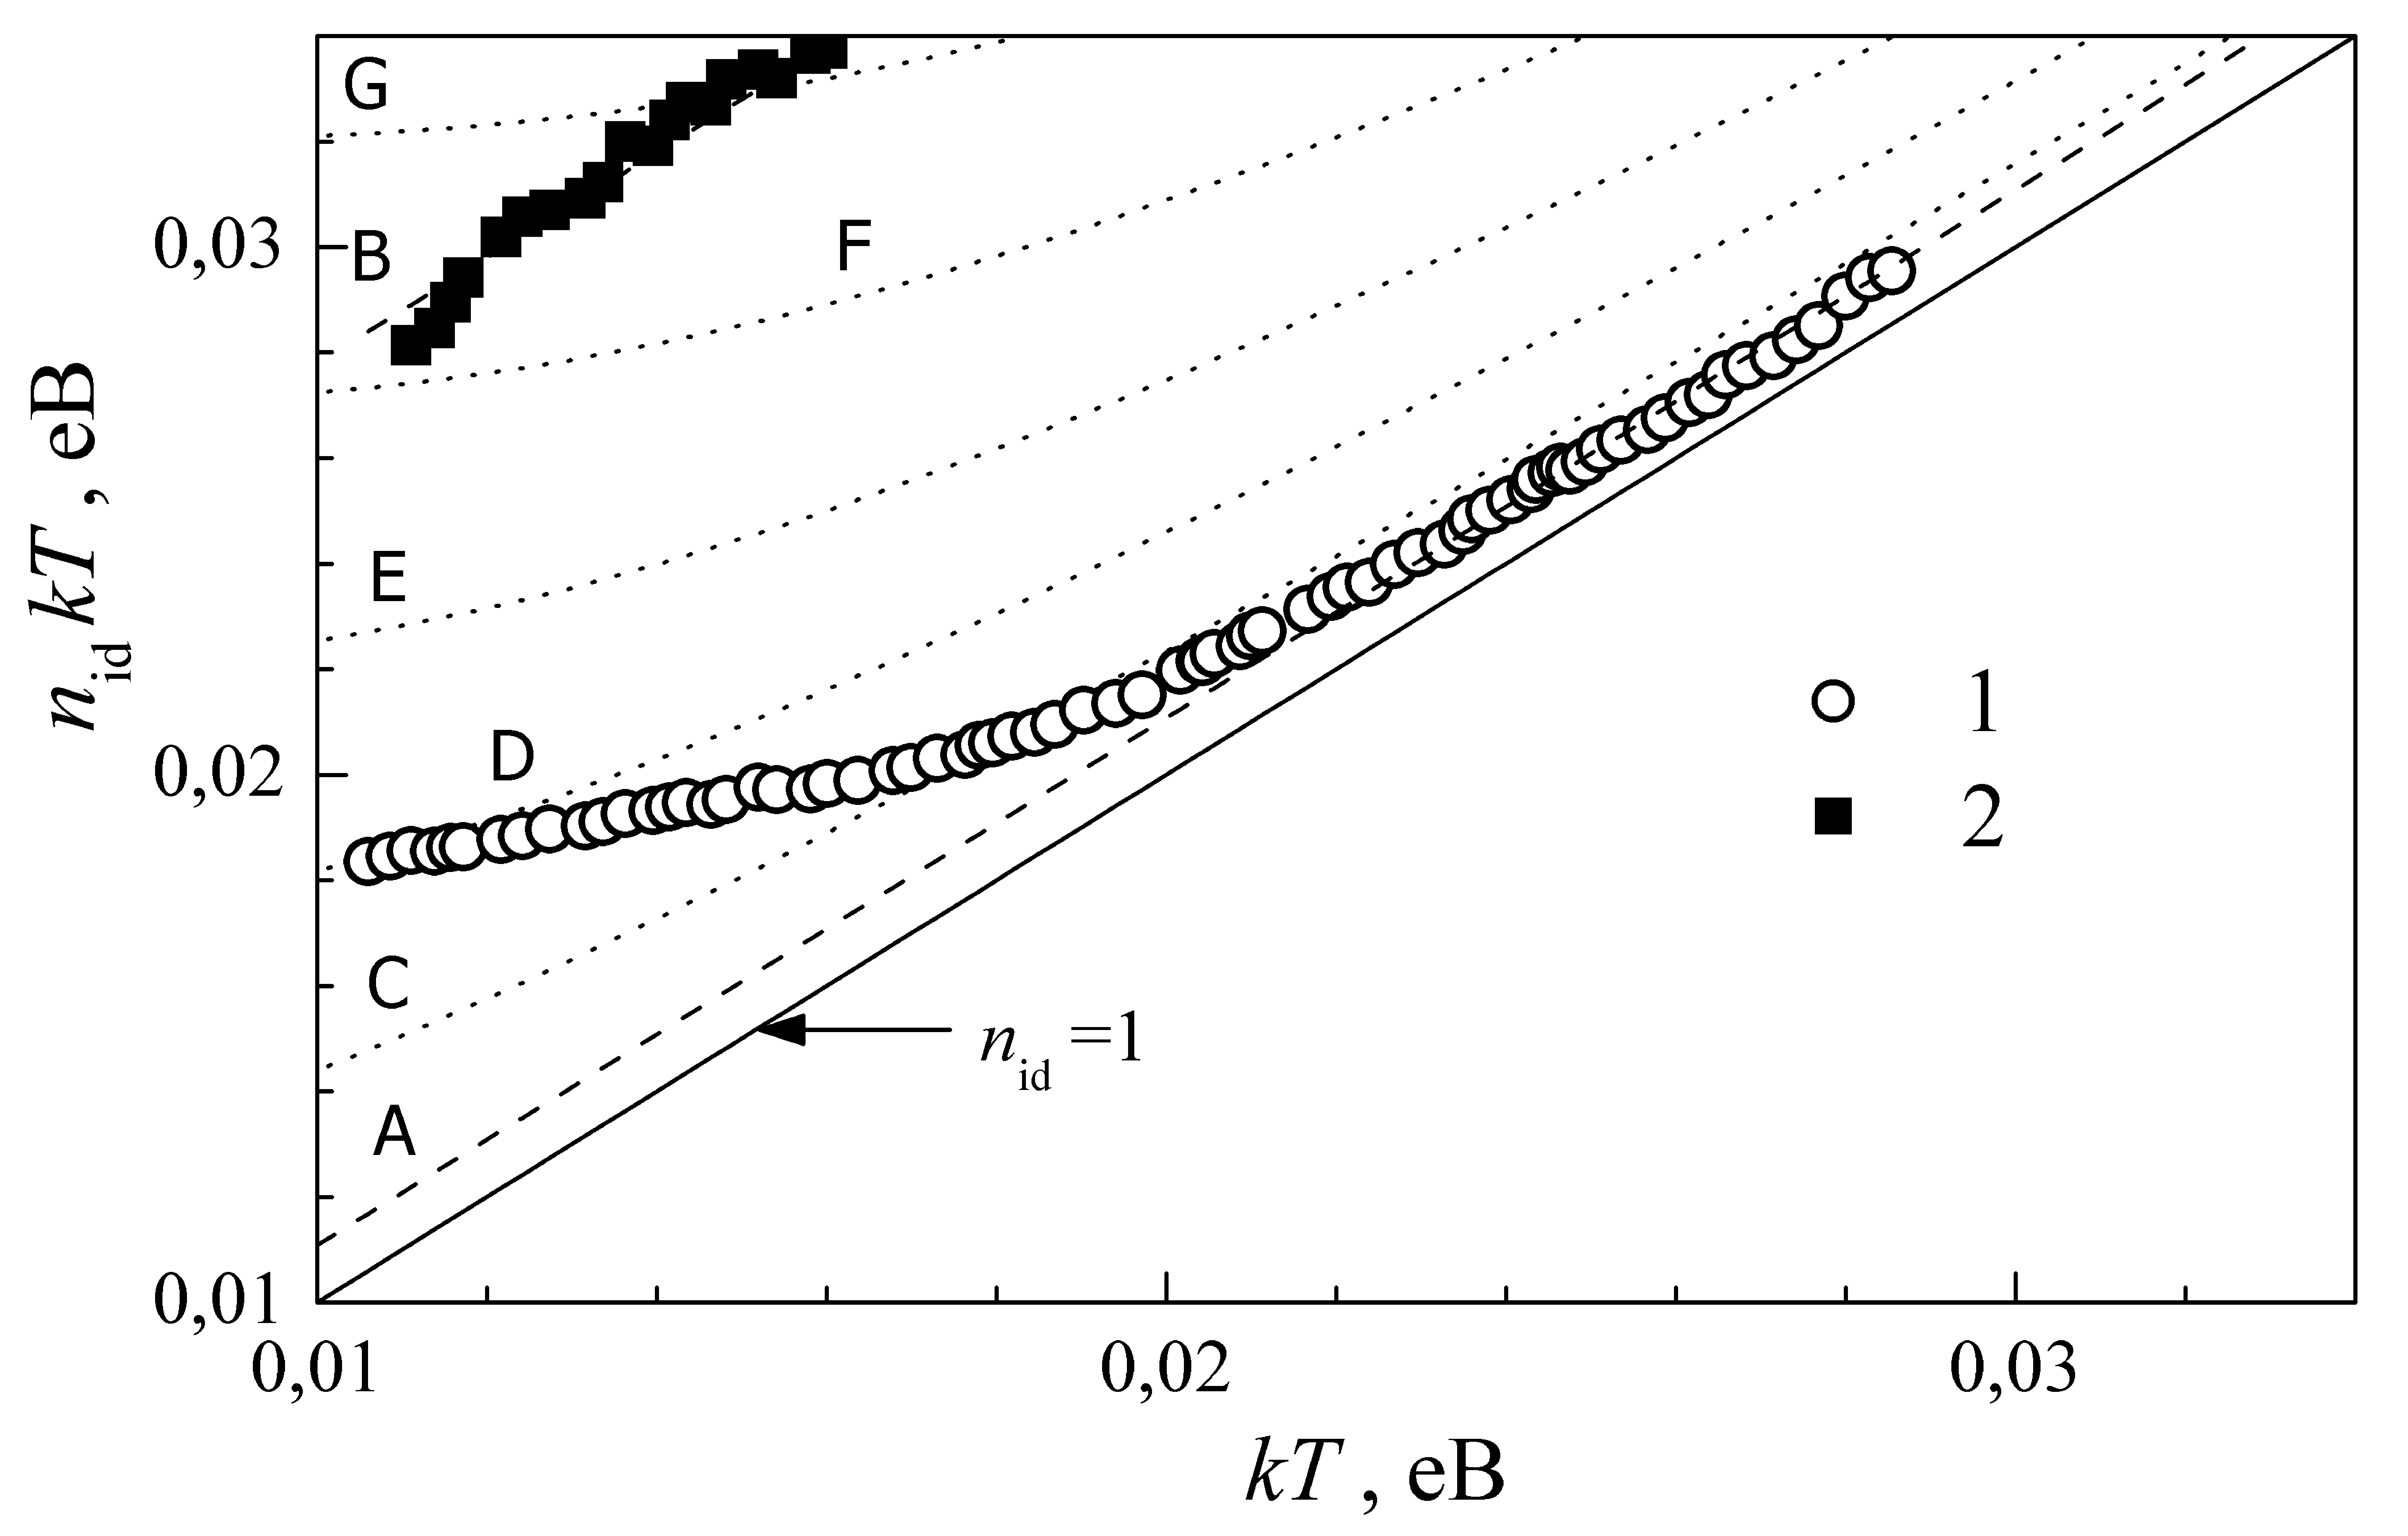
\includegraphics[width=0.6\textwidth]{figNT_SDA}
\caption{\label{figNT_SDA}
Температурна залежність оберненого нахилу ВАХ.
1 --- $n_{\mathrm{id},1}$;
2 --- $n_{\mathrm{id},2}$.
Пунктир --- теоретичні криві відповідно до формул (\ref{eqN_T:TE}) (криві А та В)
та (\ref{eqN_T:TFE}) (криві С-G).
$T_0$, K: 12 (A), 206 (B).
$E_{00}$, мВ: 12 (С), 17 (D), 22 (E), 27 (F), 32 (G).
Також наведено ідеальний випадок ($n_{\mathrm{id}}=1$) --- пряма суцільна лінія
}%
\end{figure}

На рис.~\ref{figNT_SDA} наведено експериментально отримані залежності факторів неідеальності від оберненої температури
для обох струмових компонент та декілька кривих, розрахованих із використанням виразів (\ref{eqN_T:TE}) та (\ref{eqN_T:TFE}).
Видно, що отримані дані для $n_{\mathrm{id},1}$ (при $T>220$~K) та $n_{\mathrm{id},2}$ задовільно описуються
виразом (\ref{eqN_T:TE}) при $T_0=12$~К та $T_0=206$~К, відповідно,
що свідчить на користь ТЕ як основного механізму перенесення заряду.
Зауважимо, що при ТПЕ
\begin{equation}\label{eqE00:TFE}
E_{00}^\mathrm{TFE}=\frac{\hbar}{2}\sqrt{\frac{N_d}{m^*\varepsilon_s\varepsilon_0}},
\end{equation}
($m^*$ -- ефективна маса електрону, $m^*=1,08\cdot9,11\cdot10^{-31}$~кг)
і тому для досліджених зразків та температурного діапазону очікувалось, що при домінуванні цього механізму $n_\mathrm{id}\approx1$.



Як вже згадувалося раніше, для однорідного контакту Шотткі теоретично \cite{Rhoderick1988} та експериментально \cite{Aboelfotoh,Zhua} показано,
що при підвищенні температури за умови домінування термоелектронної емісії ВБШ має зменшуватися,
причому температурні коефіцієнти змін $\Phi_b$ та  $E_g$ дуже близькі між собою.
На рис.~\ref{figFbT_SDA},а також наведена температурна залежність $E_g$, розрахована з використанням
виразу (\ref{eqEg}).
Для дослідженої структури спостерігається протилежна тенденція: ВБШ зі збільшенням температури зростає практично у всьому
діапазоні
і лише для компоненти $I_1$ поблизу кімнатної температури поведінка $\Phi_b$ нагадує $E_g$.

З іншого боку, відомо, що ВБШ, визначена за допомогою ВАХ, може відрізнятися від реальної.
Зокрема, в роботі \cite{Bozhkov} стверджується про необхідність проведення вимірів при сталому струмі через контакт
і пропонується для оцінки ефективної висоти бар'єру $\Phi_{b}^\mathrm{eff}$ використовувати вираз
\begin{equation}\label{eqBoz}
\Phi_{b}^\mathrm{eff}=n_{Ic}\Phi_b-(n_{Ic}-1)\cdot\frac{kT}{q}\cdot\ln\left(\frac{AA^*T^2}{I_c}\right),
\end{equation}
де
$n_{Ic}$ --- фактор неідеальності при певному сталому значенні струму $I_c$.
У роботі \cite{Bozhkov} також показано, що у випадку ТЕ через однорідний контакт величина $\Phi_{b}^\mathrm{eff}$ майже збігається
із реальною висотою бар'єру і має з нею однакову температурну залежність.

Результати обчислення $\Phi_{b1}^\mathrm{eff}$ для $I_{s1}$ згідно з формулою (\ref{eqBoz}) при $I_c=10^{-3}$~А показані на рис.~\ref{figFbT_SDA}, крива 3.
Видно, що хоча величина $\Phi_{b1}^\mathrm{eff}$ і змінюється в значно меншому діапазоні,
проте її температурна залежність також відрізняється від поведінки $E_g$, особливо при низьких температурах.


Якщо ТЕ є домінуючим механізмом перенесення заряду, то параметр $A^*$ може бути
визначений \cite{Rhoderick1988,Schroder2006} шляхом побудови так званої залежності Річардсона,
тобто залежності величини $\ln(I_s/T^2)$ від $(kT)^{-1}$.
Згідно з (\ref{eqFb:TE}) вона має описуватися виразом
\begin{equation}\label{eqRich}
\ln\left(\frac{I_s}{T^2}\right)=\ln(AA^*)-\frac{q\Phi_b}{kT},
\end{equation}
тобто залежність Річардсона має бути прямою, нахил якої визначається ВБШ,
я точка перетину з вертикальною віссю --- константою $A^*$.


Відповідна залежність, побудована для даних, отриманих для складової $I_1$ наведена
на рис.~\ref{figRich_SDA}, крива 1.
Видно, що лінійна залежність дійсно спостерігається, але не у всьому діапазоні температур, а у двох окремих піддіапазонах.
Шляхом апроксимації в діапазоні $(130\div220)$~К отримані значення $3,7\cdot10^{-10}$~А$\cdot$см$^{-2}\cdot$К$^{-2}$ та
$0,141$~В для сталої Річардсона та висоти бар'єру, відповідно,
для діапазону $(230\div330)$~К ---
$30$~А$\cdot$см$^{-2}\cdot$К$^{-2}$ та $0,599$~В.
Величини також наведені в табл.~\ref{tabPar:SSDA}.
Очевидно, що отримані значення сталої Річардсона суттєво відрізняються від літературних даних
для кремнію (112~А$\cdot$см$^{-2}\cdot$К$^{-2}$).


\begin{figure}
\center
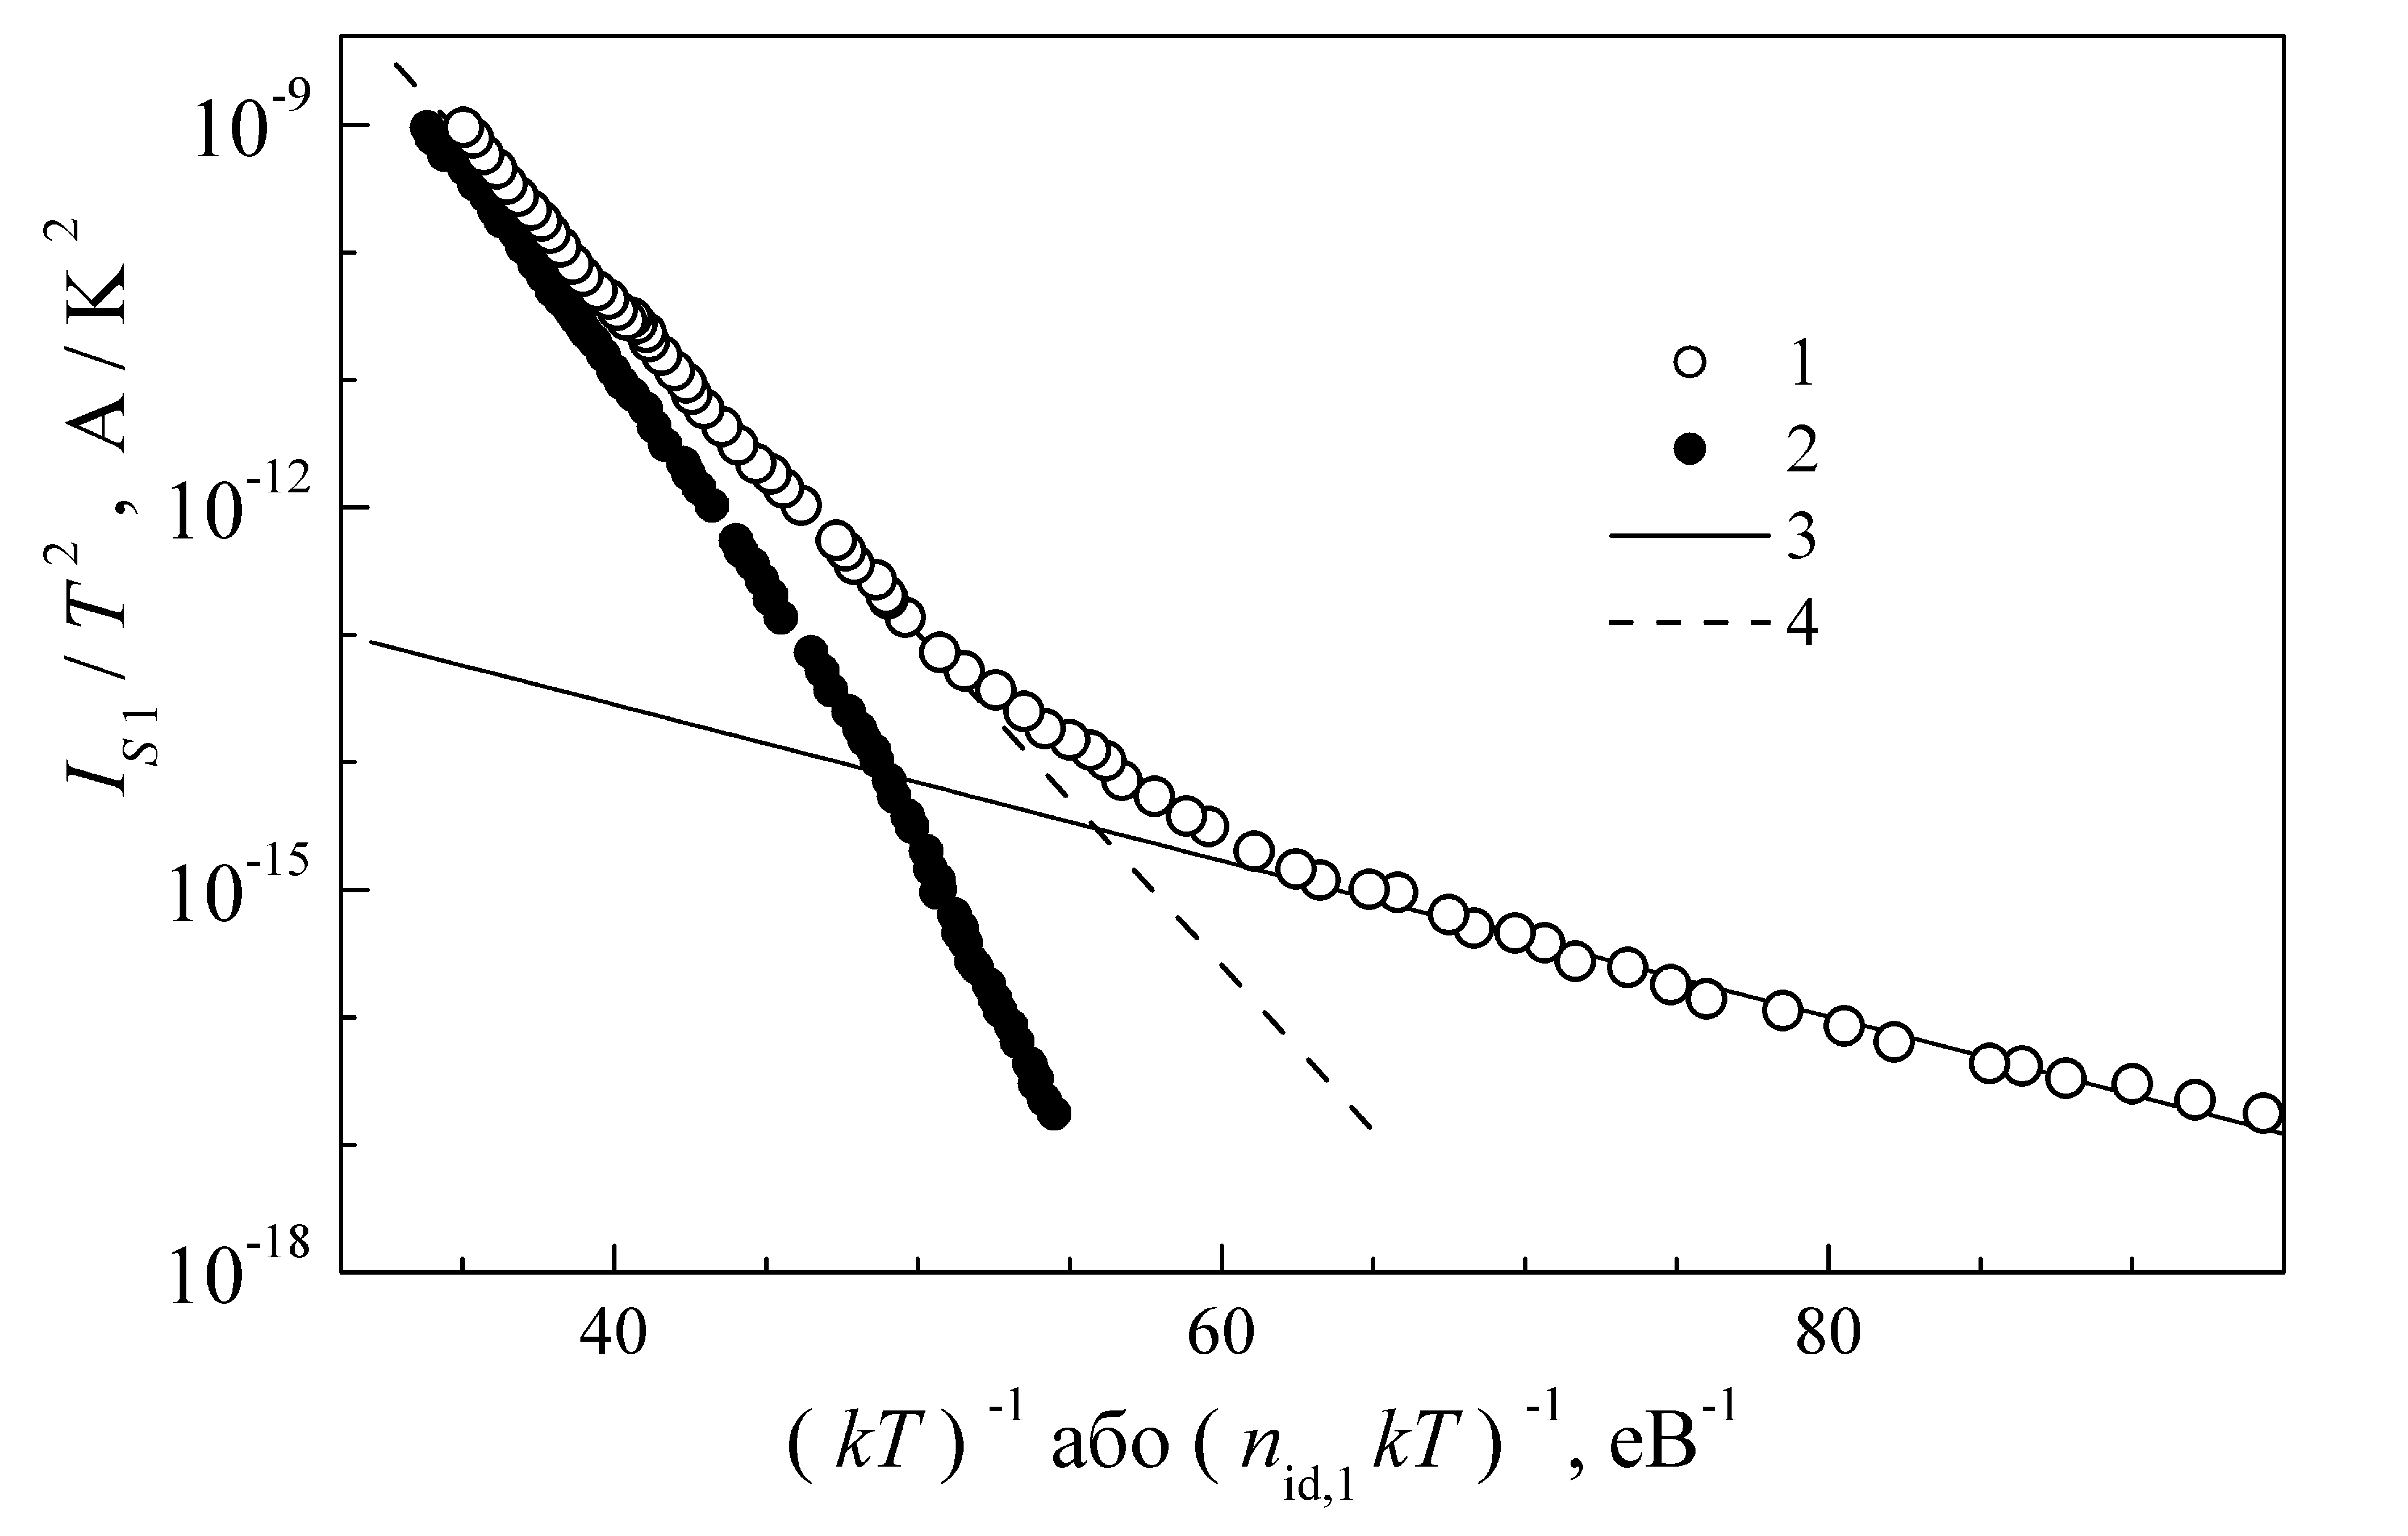
\includegraphics[width=0.7\textwidth]{figRich_SDA}
\caption{\label{figRich_SDA}
Залежності Річардсона, побудовані для високотемпературної компоненти струму $I_1$
за формулами (\ref{eqRich}) (крива 1) та (\ref{eqRichB}) (крива 2).
Прямі --- лінійна апроксимація даних кривої 1 в діапазонах $T=(130\div220)$~К (3, суцільна)
та $T=(230\div330)$~К (4, пунктир)
}%
\end{figure}



\begin{table}
\caption{\label{tabPar:SSDA}Параметри, визначені для високотемпературної складової струму неопромінених структур SSDA
}
\center
\begin{tabular}{|l|c|c|}
\hline
\multicolumn{1}{|c|}{Параметр:}& \multicolumn{2}{c|}{Температурний інтервал}\\ \cline{2-3}
метод визначення&130$\div$220~K&230$\div$330~K\\
\hline
%$A^*_R$, А$\cdot$см$^{-2}\cdot$К$^{-2}$&$3.7\cdot10^{-10}$&32\\ \hline
\multicolumn{1}{|c|}{$A^*$, А$\cdot$см$^{-2}\cdot$К$^{-2}$:}&&\\
залежність Річардсона (\ref{eqRich})&$(3,7\pm0,8)\cdot10^{-10}$&$32\pm10$\\
видозмінена залежність Річардсона (\ref{eqRichB})&$(3,0\pm0,6)\cdot10^{8}$&$40\pm8$\\
модифікована залежність Річардсона (\ref{eqRich:Mod})&$122\pm20$&$112\pm8$\\
література  \cite{Schroder2006}& \multicolumn{2}{c|}{$\,\,\,\,\,\,\,\,\,\,\,\,$   112}\\ \hline
\multicolumn{1}{|c|}{$\Phi_b$, мВ:}&&\\
залежність Річардсона (\ref{eqRich})&141$\pm$4&599$\pm$3\\
видозмінена залежність Річардсона (\ref{eqRichB})&1090$\pm$10&751$\pm$5\\
залежність $\Phi_b=f(\frac{1}{2kT})$&872$\pm$4&663$\pm$3\\
залежність $\Phi_b=f(n_\mathrm{id})$&646$\pm$5&640$\pm$20\\
модифікована залежність Річардсона (\ref{eqRich:Mod})&872$\pm$3&662$\pm$3\\
ВФХ &&683$\pm$2\\
\hline
залежність $\Phi_b=f(\frac{1}{2kT})$:&&\\
\multicolumn{1}{|c|}{$\sigma_{\Phi0}$, мВ} &99$\pm$1&40$\pm$5\\
\multicolumn{1}{|c|}{$\rho_2$, $10^{-2}$} &33$\pm$1&12$\pm$1\\
\multicolumn{1}{|c|}{$\rho_3$, мВ }&17,0$\pm$0,3&8,0$\pm$0,3\\
\hline
\end{tabular}
\end{table}



У роботі \cite{Aldemir} показано, що
при суттєвому відхиленні від ідеальності (величина $n_\mathrm{id}$ значно перевищує одиницю)
для визначення $A^*$ можна також використовувати \cite{Aldemir,Mohan} видозмінену залежність Річардсона,
відкладаючи по осі абсцис не $(kT)^{-1}$, а $(n_\mathrm{id} kT)^{-1}$:
\begin{equation}\label{eqRichB}
\ln\left(\frac{I_s}{T^2}\right)=\ln(AA^*)-\frac{q\Phi_b}{n_\mathrm{id}kT},
\end{equation}
Проте для нашого випадку і видозмінена залежність Річардсона (рис.~\ref{figRich_SDA}, крива 2) не є лінійною для всього
температурного діапазону, а отримані значення $A^*$ (табл.~\ref{tabPar:SSDA}) суттєво відрізняються
від табличного.

Узагальнюючи, необхідно визнати, що отримані результати неможливо пояснити з погляду теорії ТЕ через однорідний контакт.


З іншого боку, відмінності між експериментально виявленою температурною залежністю ВБШ та очікуваною теоретично нерідко
пов'язують із неоднорідністю межі розділу між металом та напівпровідником \cite{Dokme}.
Впливу неоднорідності можна позбутися розглядаючи ВБШ за умови плоских зон (<<flat band condition>>) $\Phi_{b}^\mathrm{FB}$:
\begin{equation}
\label{eqFbfb}
\Phi_{b}^\mathrm{FB}=n_\mathrm{id}\Phi_{b}-(n_\mathrm{id}-1)V_n\,,
\end{equation}
де
\begin{equation}
\label{eqVn}
qV_n=kT\ln\left(\frac{N_c}{N_d}\right)
\end{equation}
різниця енергій між дном зони провідності та положенням рівня Фермі в об'ємі напівпровідника,
так званий <<bulk potential>>.
На рис.~\ref{figFbfb_SDA} наведена температурна залежність $\Phi_{b}^\mathrm{FB}$, розрахована для високотемпературної компоненти $I_1$.
Зауважимо, що на рисунку також наведена температурна залежність ширини забороненої зони, причому
масштаби осей $\Phi_{b}^\mathrm{FB}$ та $E_g$ однакові.
З рисунка видно, що поведінка ВБШ в наближенні плоских зон та ширини забороненої зони дуже подібні.
Це свідчить, що механізмом перенесення заряду в досліджуваних структурах може бути ТЕ через неоднорідний бар'єр.


\begin{figure}
\center
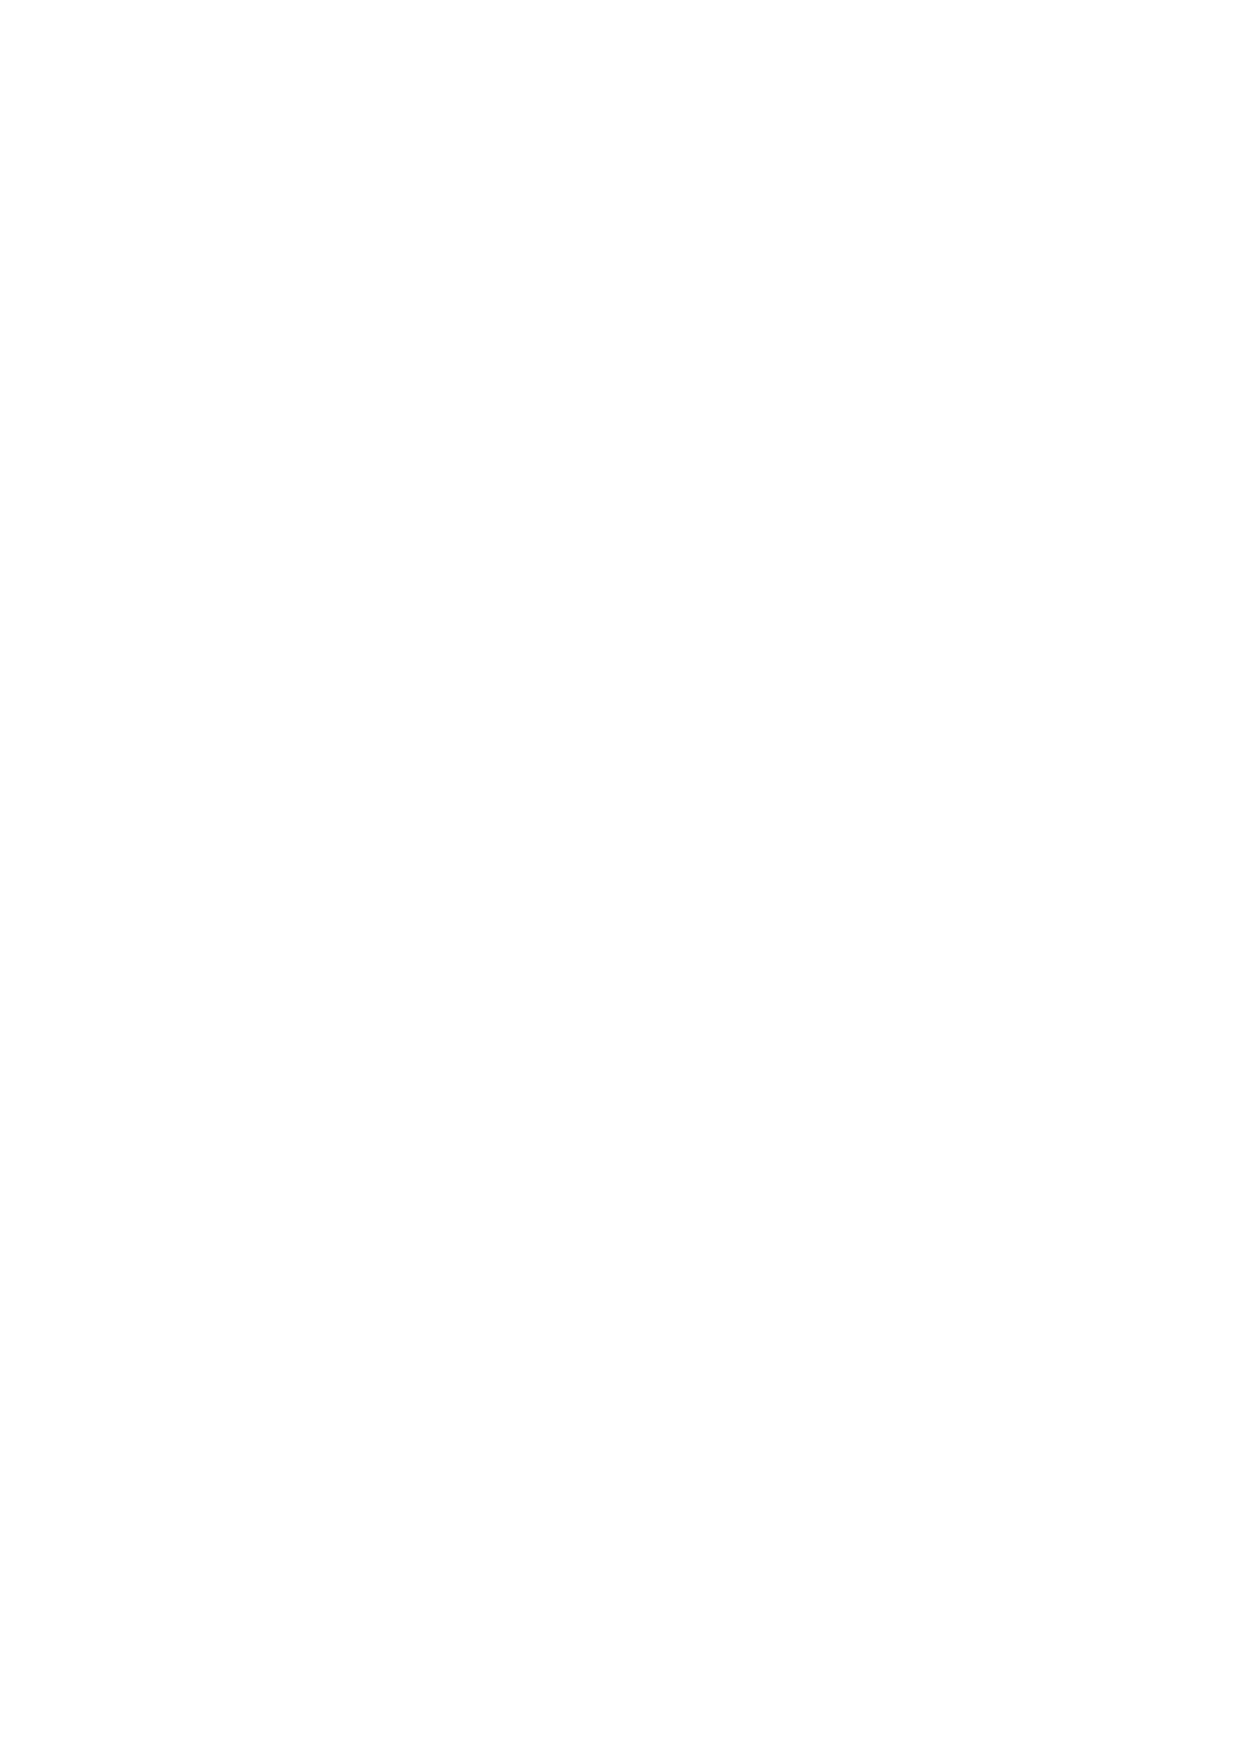
\includegraphics[width=0.55\textwidth]{figFbfb_SDA}
\caption{\label{figFbfb_SDA}
Температурні залежності ВБШ в наближені плоских зон (точки, права вісь), розрахованої
для високотемпературної компоненти струму $I_1$, та ширина забороненої зони (пунктир, ліва вісь)
}%
\end{figure}

У літературі для пояснення експериментально отриманих ВАХ структур МН використовуються два
підходи \cite{Sarpatwari, Tascioglu2010, Yildirim2010, Mamor, Iucolano2007JAP, Iucolano2007APL}, які дозволяють
%\cite{Sarpatwari, Aydemir, Turut, Mamor, Iucolano, Iucolano2}.
врахувати неоднорідність бар'ру Шотткі,
схематично ілюстровані за допомогою рис.~\ref{figFbModel}.
Згідно з першим підходом, запропонованим в \cite{Werner}, вважається, що властивості контакту між металом та напівпровідником
змінюються від точки до точки (рис.~\ref{figFbModel},а), а просторовий розподіл ВБШ  може бути описаний за допомогою функції Гауса:
\begin{equation}\label{eqFbWerner}
  P(\Phi_{b}^j)=\frac{1}{\sigma_\Phi\sqrt{2\pi}}\exp\left[-\frac{(\Phi_{b}^j-\overline{\Phi}_{b})^2}{2\sigma_\Phi^2}\right]\,,
\end{equation}
де
$P(\Phi_{b}^j)$ --- ймовірність того, що значення висоти бар'єру в певній точці дорівнює $\Phi_{b}^j$,
$\overline{\Phi}_{b}$ --- середнє значення ВБШ,
$\sigma_\Phi$ --- стандартне відхилення висоти бар'єру, показник однорідності контакту.
Також вважається, що $\overline{\Phi}_{b}$ та $\sigma_\Phi$ залежать
від прикладеної напруги і польова залежність може бути описана лінійними функціями

\begin{equation*}
   \overline{\Phi}_{b}(V)=\Phi_{b}^0+\rho_2\,V\,,\quad \sigma_\Phi^2(V)=\sigma_{\Phi0}^2+\rho_3\,V\,,
\end{equation*}
%\begin{equation}\label{eqFbV}
%   \overline{\Phi}_{b}(V)=\Phi_{b}^0+\rho_2\,V\,,
%\end{equation}
%\begin{equation}\label{eqNV}
%   \sigma_\Phi^2(V)=\sigma_{\Phi0}^2+\rho_3\,V\,,
%\end{equation}
%\begin{eqnarray}
%  \label{eqFbV} \overline{\Phi}_{b}(V)&=&\Phi_{b}^0+\rho_2\,V\,, \\
%  \label{eqNV} \sigma_\Phi^2(V)&=&\sigma_{\Phi0}^2+\rho_3\,V\,,
%\end{eqnarray}
де
$\Phi_{b}^0$ та $\sigma_{\Phi0}$ відповідають нульовому зміщенню,
а  $\rho_2$ та $\rho_3$ --- певні коефіцієнти.

\begin{figure}
\center
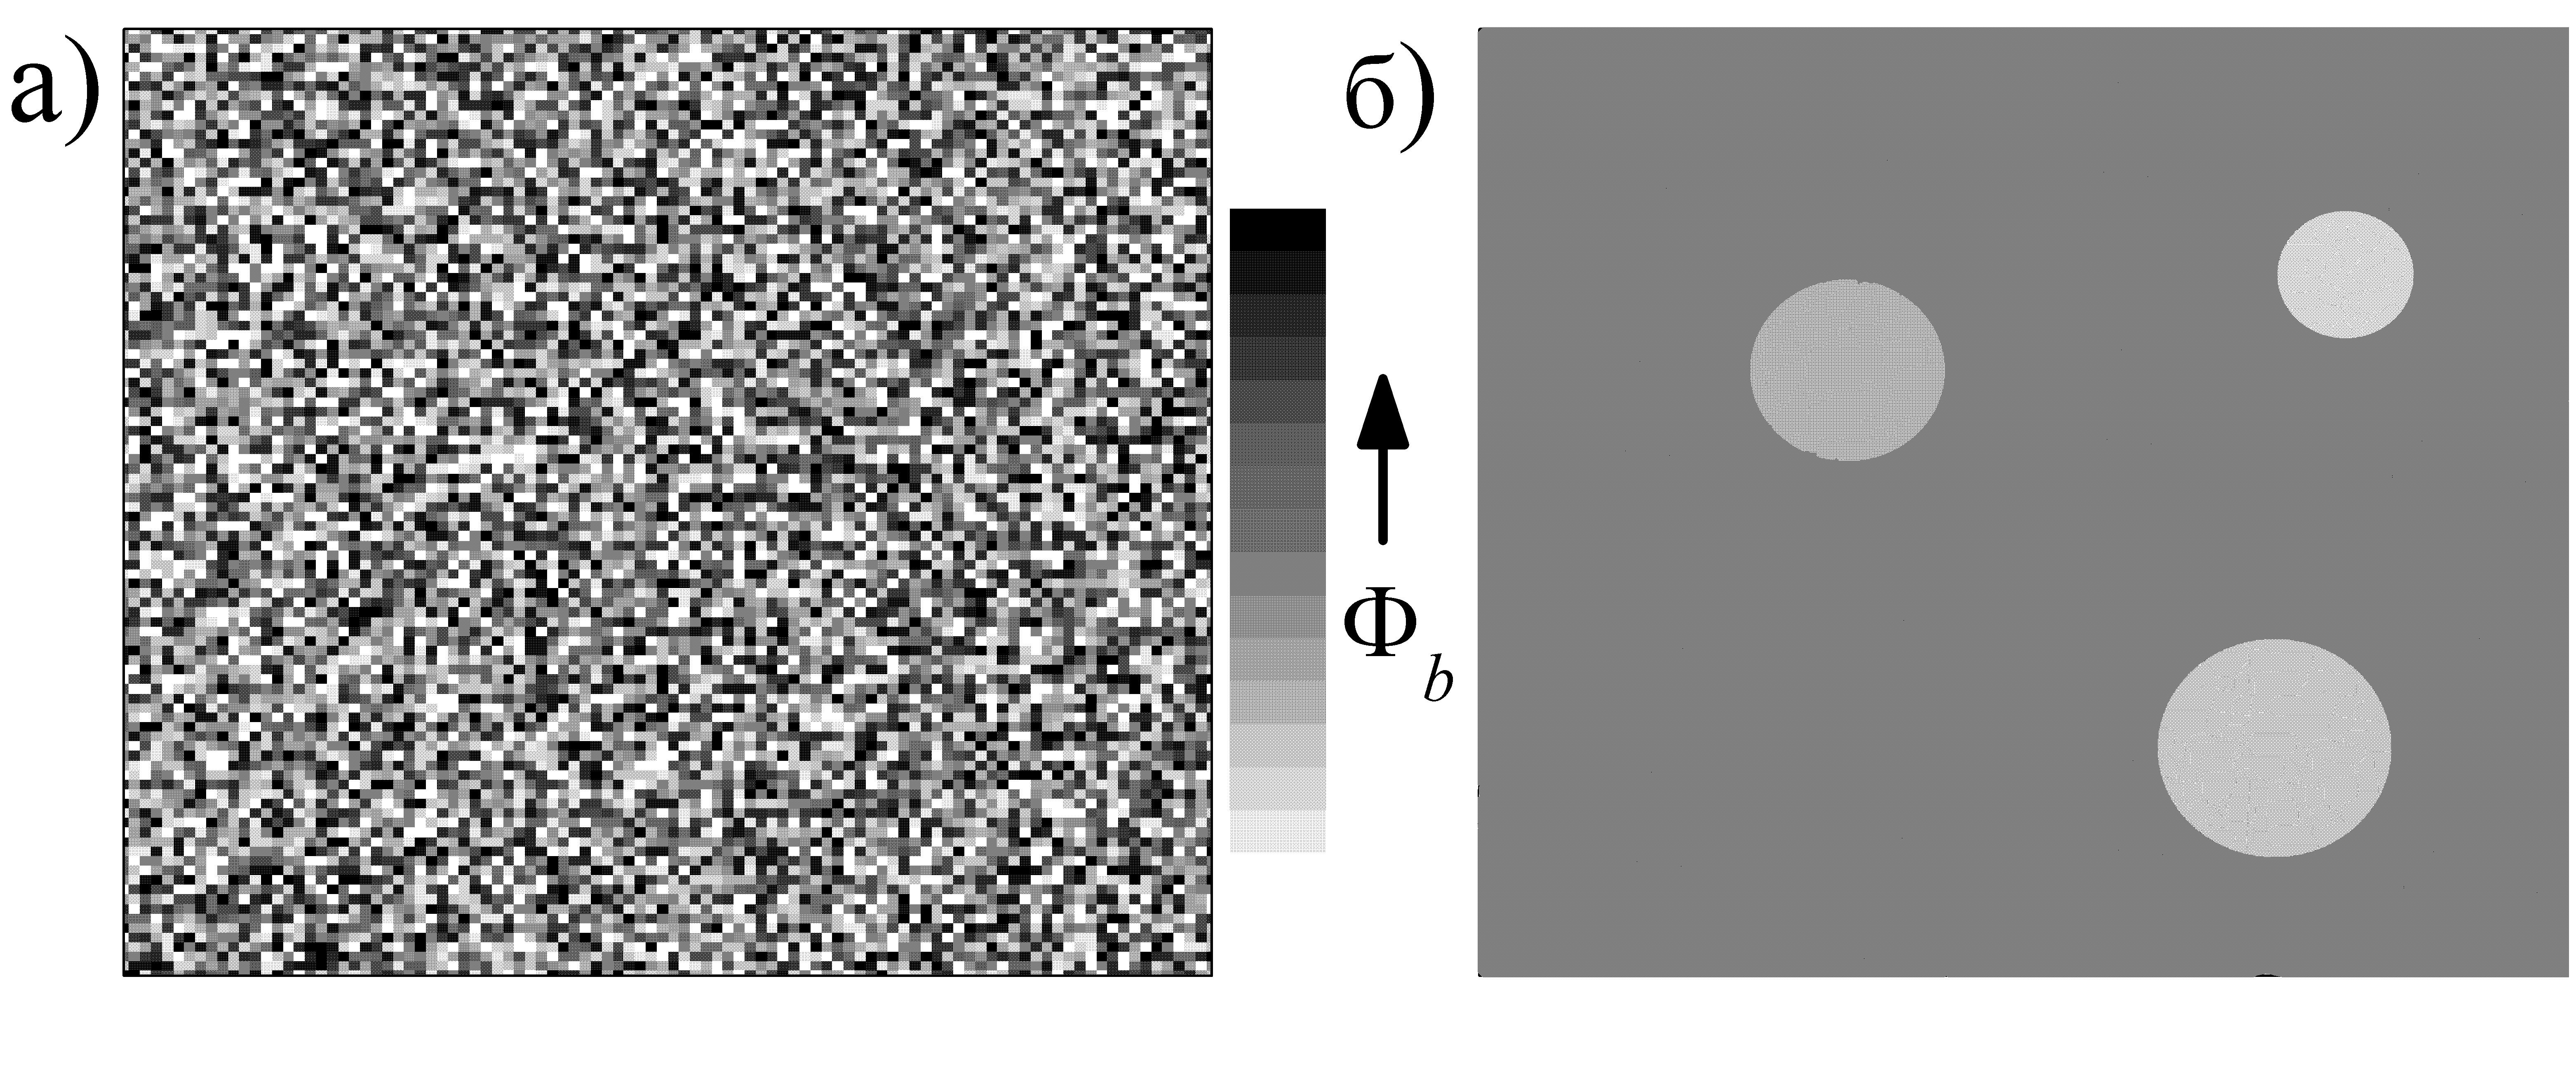
\includegraphics[width=0.9\textwidth]{figFbModel}
\caption{\label{figFbModel}
Моделі неоднорідного по площі контакту МН:
а --- ВБШ визначається розподілом Гауса;
б --- однорідний бар'єр із патчами
}%
\end{figure}

Ця теорія передбачає,
що фактор неідеальності, який визначається за нахилом ВАХ, і ВБШ, розрахована за допомогою виразу (\ref{eqFb:TE}),
пов'язані з $\rho_2$ та $\rho_3$ і
$\Phi_{b}^0$ та $\sigma_{\Phi0}$, відповідно \cite{Werner,Tascioglu2010,Yildirim2010,Mamor,Soylu}:

\begin{eqnarray}
  \label{eqNidT} \frac{1}{n_\mathrm{id}}-1&=&\rho_2+\frac{q\rho_3}{2kT}\,, \\
  \label{eqFb0T} \Phi_b&=&\Phi_b^0-\frac{q\sigma^2_{\Phi0}}{2kT}.
\end{eqnarray}

%\begin{equation}\label{eqNidT}
%  \frac{1}{n_\mathrm{id}}-1=\rho_2+\frac{q\rho_3}{2kT}\,,
%\end{equation}
%\begin{equation}\label{eqFb0T}
%\Phi_b=\Phi_b^0-\frac{q\sigma^2_{\Phi0}}{2kT}.
%\end{equation}

Відповідно до іншої моделі неоднорідного контакту Шотткі \cite{Sullivan,Tung:PhysRev,Tung:MSE,Tung:ApplPhysRev}, ВБШ вважається однаковою на всій межі МН,
окрім невеликих за площею ділянок (так званих патчів), де значення ВБШ менше --- рис.~\ref{figFbModel},б.
Ділянки можуть відрізнятися між собою площею та висотою бар'єру, причому розподіл параметру, який
характеризує окремий патч:
\begin{equation}\label{eqGammaP}
  \gamma_p=3\left(R_p^2\Delta_p/4\right)^{1/3},
\end{equation}
($\Delta_p$ та $R_p$ --- зниження висоти бар'єру в області патча та його розмір, відповідно)
також описується функцією Гауса зі стандартним відхиленням $\sigma_{\gamma p}$.


У ряді робіт \cite{Iucolano2007JAP, Iucolano2007APL} показано, що ці теорії можуть бути використані сумісно,
причому за наявності патчів також має виконуватися співвідношення (\ref{eqFb0T}),
причому величина $\Phi_b^0$ має зміст ВБШ за межами патчів (в однорідній області),
а $\sigma_{\Phi0}$ пов'язаний з розподілом параметрів патчів:
\begin{equation}\label{eqGigFSigG}
  \sigma_{\Phi0}=\sigma_{\gamma p}\left(\frac{qV_{bb}N_d}{\varepsilon\varepsilon_0}\right)^{1/3}.
\end{equation}
%де
%$\sigma_{\gamma p}$ --- стандартне відхилення для сукупності патчів параметра $\gamma_p$, який
%характеризує окремий патч:
%\begin{equation}\label{eqGammaP}
%  \gamma_p=3\left(\frac{R_p^2\Delta_p}{4}\right)^{1/3},
%\end{equation}
%$\Delta_p$ та $R_p$ --- зниження висоти бар'єру в області патча та його розмір, відповідно.
Крім того, показано \cite{Sullivan,Tung:PhysRev,Iucolano2007JAP, Iucolano2007APL}, що за наявності неоднакових патчів
температурна залежність фактора неідеальності має описуватися виразом (\ref{eqN_T:TE}), причому
\begin{equation} \label{eqN_T0}
T_0=\frac{q\sigma_{\Phi0}^2}{3kV_{bb}}\,,
\end{equation}
де
$V_{bb}=(\Phi_b^0-V_n-V)$ --- вигин зон напівпровідника поблизу контакту.

Зауважимо, що підхід, який передбачає  врахування неоднорідності
інтерфейсу  широко використовується  при аналізі ВАХ різноманітних структур із контактом Шотткі
\cite{Soylu,GELCZUK2014,Mohan,JYOTHI2015,DURMUS2014,KHURE2015,OZAVCI2013,Cetin2005,Karatas:2006NIMA,Sarpatwari,
Tascioglu2010,Yildirim2010,Mamor,Iucolano2007JAP,Iucolano2007APL,Li2016}.

Залежності, побудовані відповідно до виразів (\ref{eqNidT}) та (\ref{eqFb0T}) наведені на рис.\ref{figFbNT1_SDA}.
Видно, що дійсно спостерігається лінійна залежність,
у двох окремих температурних діапазонах (130$\div$220)~К та (230$\div$330)~К.
Визначені шляхом лінійної апроксимації величини $\Phi_{b}^0$, $\sigma_{\Phi0}$, $\rho_2$ та $\rho_3$ для кожного з діапазонів
наведено в табл.~\ref{tabPar:SSDA}.

\begin{figure}
\center
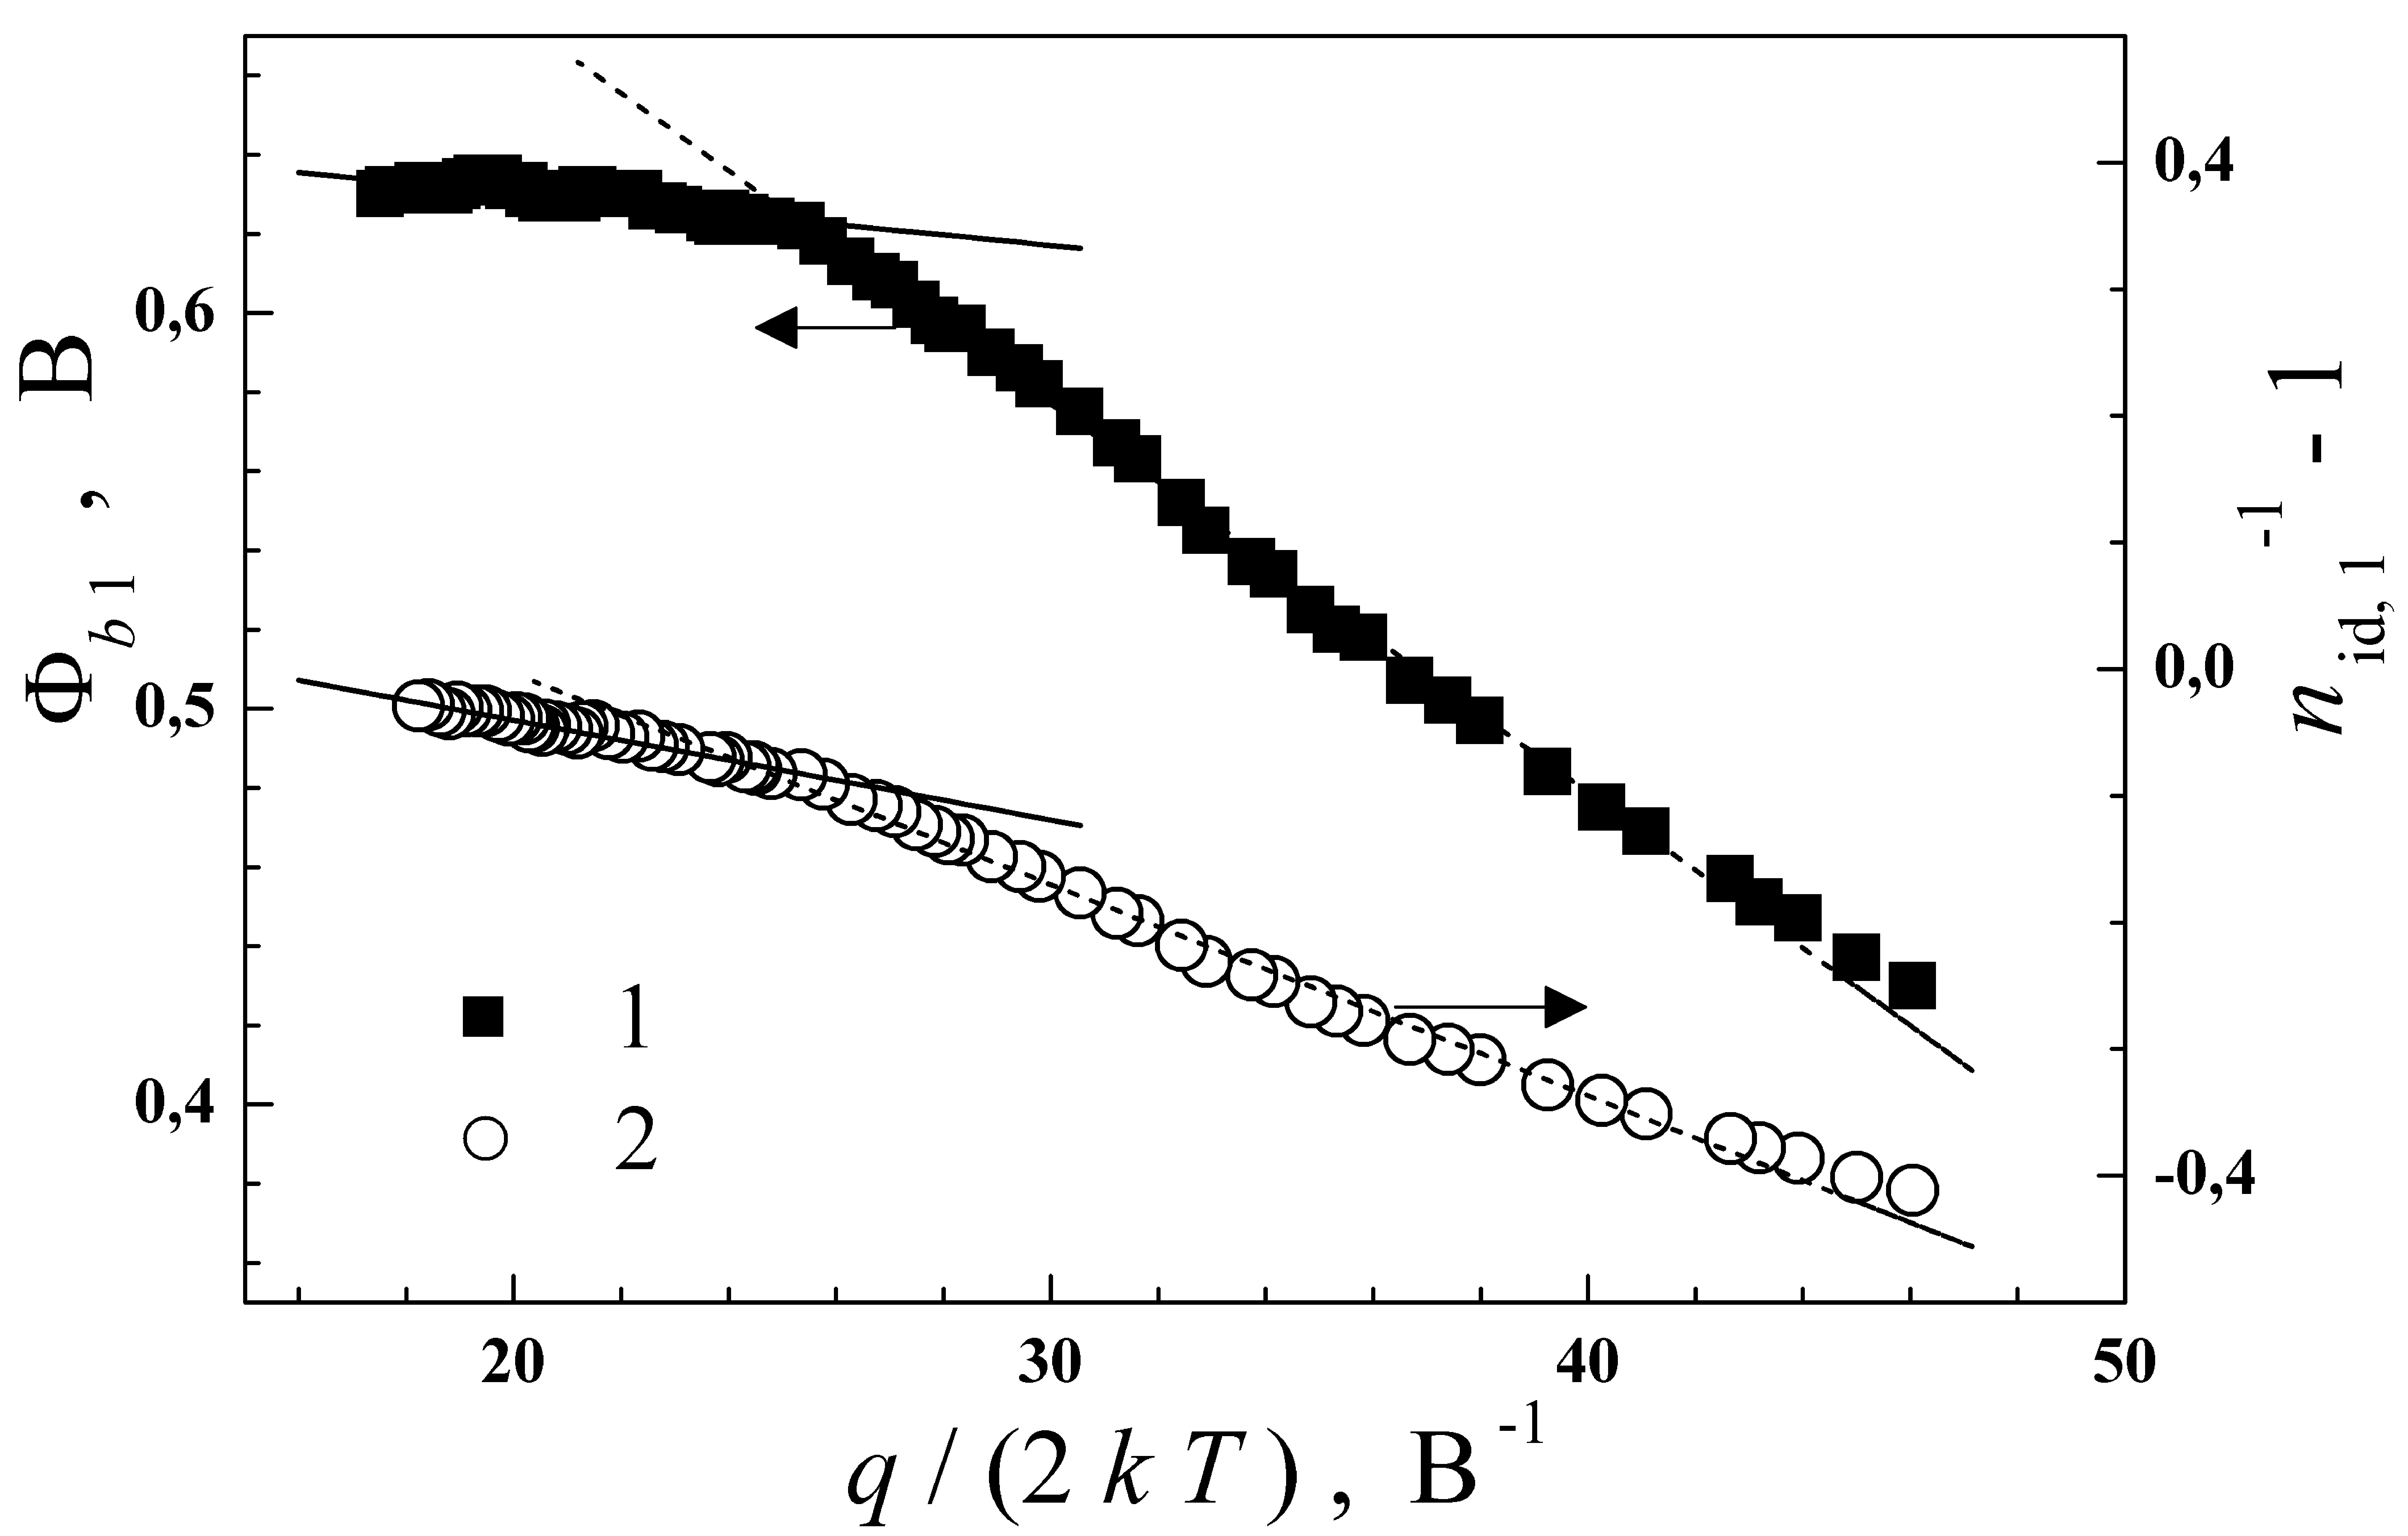
\includegraphics[width=0.65\textwidth]{figFbNT1_SDA}
\caption{\label{figFbNT1_SDA}
Залежності величин $\Phi_{b1}$ (крива 1) та $n_{\mathrm{id},1}^{-1}-1$ (крива 2) від оберненої температури.
Прямі --- лінійна апроксимація у діапазонах $T=(130\div220)$~К (суцільна) та $T=(230\div330)$~К (пунктир)
}%
\end{figure}

Використовуючи вираз (\ref{eqN_T0}) та значення $\Phi_{b}^0\simeq0.663$~В, $\sigma_{\Phi0}\simeq0.04$~В
була розрахована характерна температура $T_{0,teor}\approx11$~К, яка очікується в рамках моделі контакту Шотткі з локальними неоднорідностями
для діапазону (230$\div$330)~К.
Ця величина досить близька до значення $T_{0,exp}\approx12$~К, отриманого експериментально (рис.~\ref{figNT_SDA}) у цьому ж діапазоні.
Ще одним аргументом на користь того, що струм $I_1$ може бути описаний в рамках моделі ТЕ через неоднорідний контакт є якісний збіг
поведінки $n_{\mathrm{id},1}$ при низьких температурах (рис.~\ref{figNT_SDA}) з очікуваною теоретично (\cite[Fig.11(b)]{Tung:PhysRev}).


У роботах  \cite{Tung:PhysRev,Sarpatwari,Schmitsdorf} показано, що для випадку
контакту з локальними неоднорідностями залежність між отриманими з аналізу ВАХ величинами $\Phi_b$ та $n_\mathrm{id}$ має бути лінійною,
причому $\Phi_{b}^0=\Phi_{b}+\Delta\Phi_b^\mathrm{IF}$ при $n=n_\mathrm{id}^\mathrm{IF}$
де $n_\mathrm{id}^\mathrm{IF}$ ---  величина фактора неідеальності з врахуванням впливу сил зображення,
$\Delta\Phi_b^\mathrm{IF}$ --- зниження бар'єру внаслідок дії сил зображення,
згідно з \cite{Sarpatwari}

\begin{equation*}
n_\mathrm{id}^\mathrm{IF}\approx 1+\frac14\left[\frac{q^3N_d}{8\pi^2\varepsilon^2\varepsilon_0^2V^3_{bb}}\right]^{1/4},\quad
\Delta\Phi_b^\mathrm{IF}\approx \left(\frac{q^3N_d\,V_{bb}}{8\pi^2\varepsilon^2\varepsilon_0^2}\right)^{1/4}.
\end{equation*}


%\begin{equation}\label{eqN:IF}
%n_\mathrm{id}^\mathrm{IF}\approx 1+\frac14\left[\frac{q^3N_d}{8\pi^2\varepsilon^2\varepsilon_0^2V^3_{bb}}\right]^{1/4},
%\end{equation}
%\begin{equation}\label{eqFb:IF}
%\Delta\Phi_b^\mathrm{IF}\approx \left(\frac{q^3N_d\,V_{bb}}{8\pi^2\varepsilon^2\varepsilon_0^2}\right)^{1/4}.
%\end{equation}
На залежності $\Phi_{b1}$ від $n_{\mathrm{id},1}$ (рис.~\ref{figFbN_SDA}), як і в попередній випадках,
спостерігаються дві лінійні області зі зламом при $T\approx225$~К.
Шляхом екстраполяції отримано, що $\Phi_b^0$ дорівнює 0,64~В в обох діапазонах, див. табл.~\ref{tabPar:SSDA}.
Зауважимо, що згідно з \cite{Sarpatwari,Schmitsdorf}
при зниженні температури зростає роль проходження струму через патчі і, хоча лінійність між  $\Phi_b$ та $n_\mathrm{id}$ зберігається,
екстрапольоване значення ВБШ не буде дорівнювати висоті бар'єру в однорідній області.
Саме цим пояснюється відмінність величини $\Phi_b$, визначеної за залежністю
$\Phi_b=f(n_\mathrm{id})$ в низькотемпературному діапазоні, від інших,
отриманих для (130$\div$220)~К із використанням моделі неоднорідного бар'єру (табл.~\ref{tabPar:SSDA}).

\begin{figure}
\center
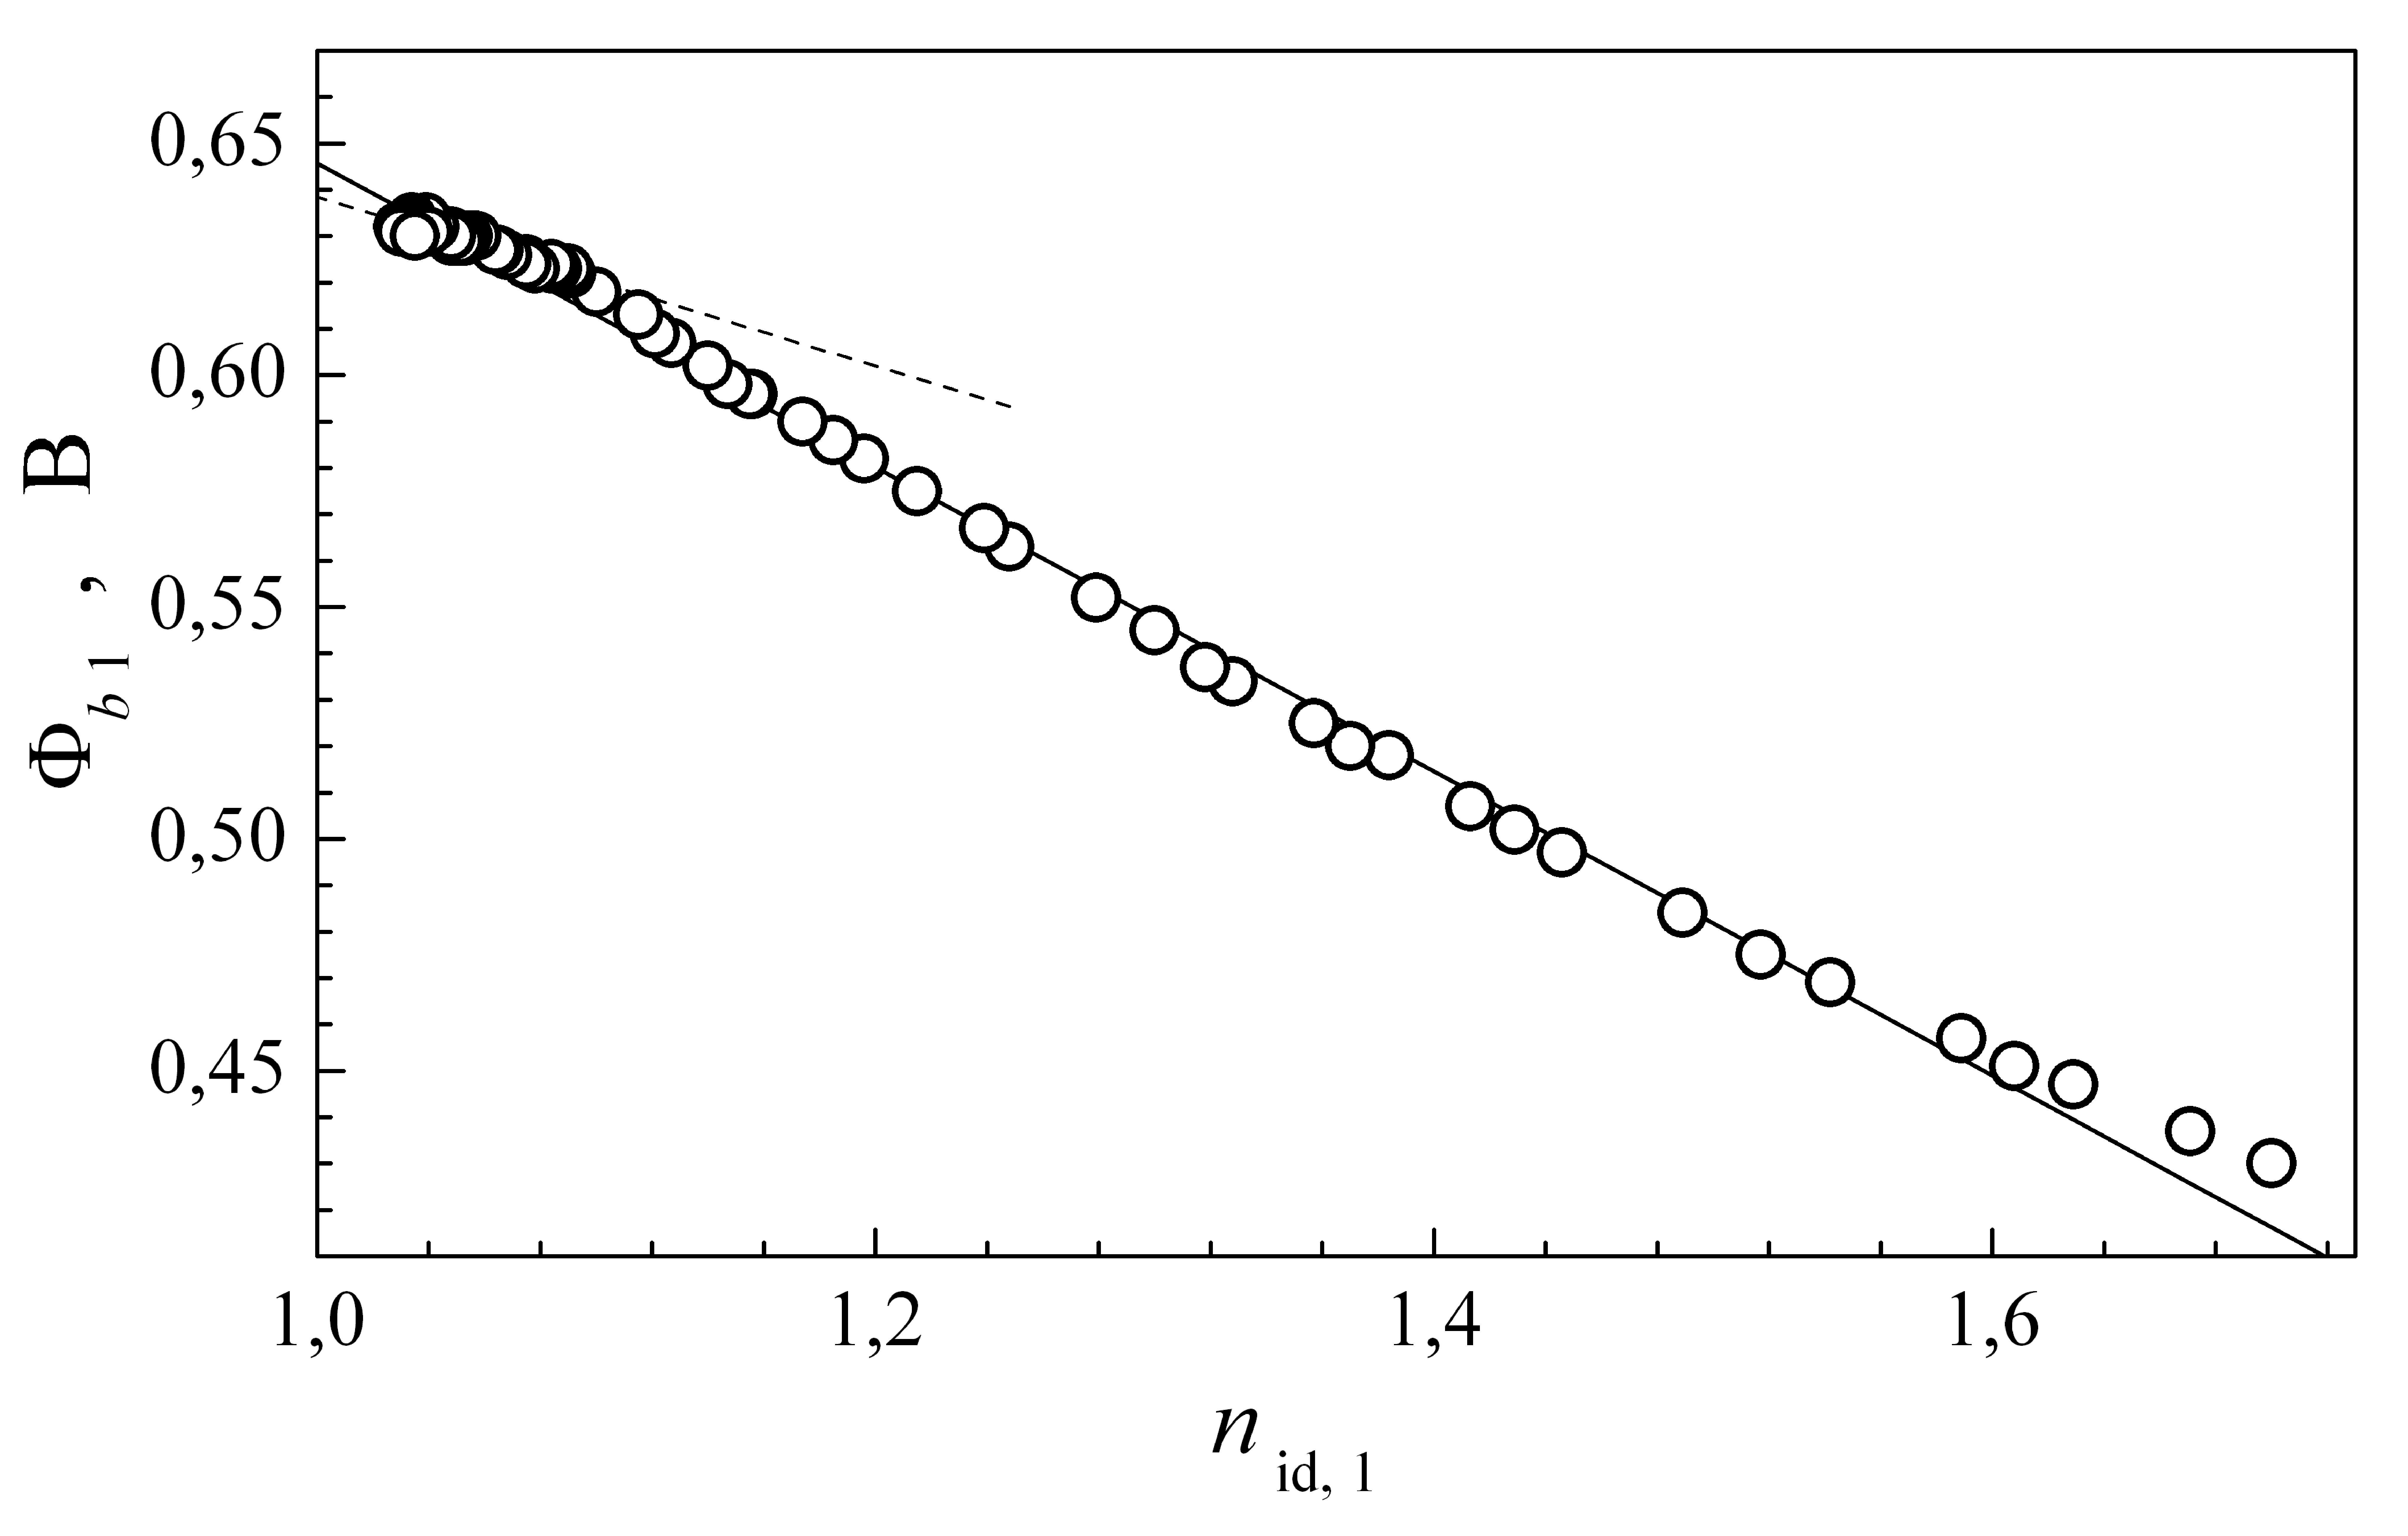
\includegraphics[width=0.65\textwidth]{figFbN_SDA}
\caption{\label{figFbN_SDA}
Залежність ВБШ від фактора неідеальності для високотемпературної компоненти струму $I_1$.
Прямі --- лінійна апроксимація у діапазонах (130$\div$220)~К (суцільна) та (230$\div$330)~К (пунктир)
}%
\end{figure}

У випадку неоднорідного бар'єру Шотткі $A^*$ може бути визначена за
допомогою модифікованої залежності Річардсона \cite{Tascioglu2010old,Yildirim2010}:
\begin{equation} \label{eqRich:Mod}
\ln\left(\frac{I_s}{T^2}\right)-\left(\frac{q^2\sigma_{\Phi0}^2}{2k^2T^2}\right)=\ln(AA^*)-\frac{q\Phi_b^0}{kT}.
\end{equation}
Відповідні графіки, побудовані з використанням отриманих значень $\sigma_{\Phi,0}$ показано на рис.~\ref{figRichM_SDA}.
Лінійна апроксимація отриманих кривих у температурних діапазонах, відповідних тим, де були визначені стандартні відхилення
дозволили оцінити середнє значення ВБШ та сталу Річардсона.
Дані наведено в табл.~\ref{tabPar:SSDA}.
Зауважимо, що величини $A^*$, отримані в різних діапазонах температур в межах похибок збігаються як між собою, так і з літературними даними.


\begin{figure}
\center
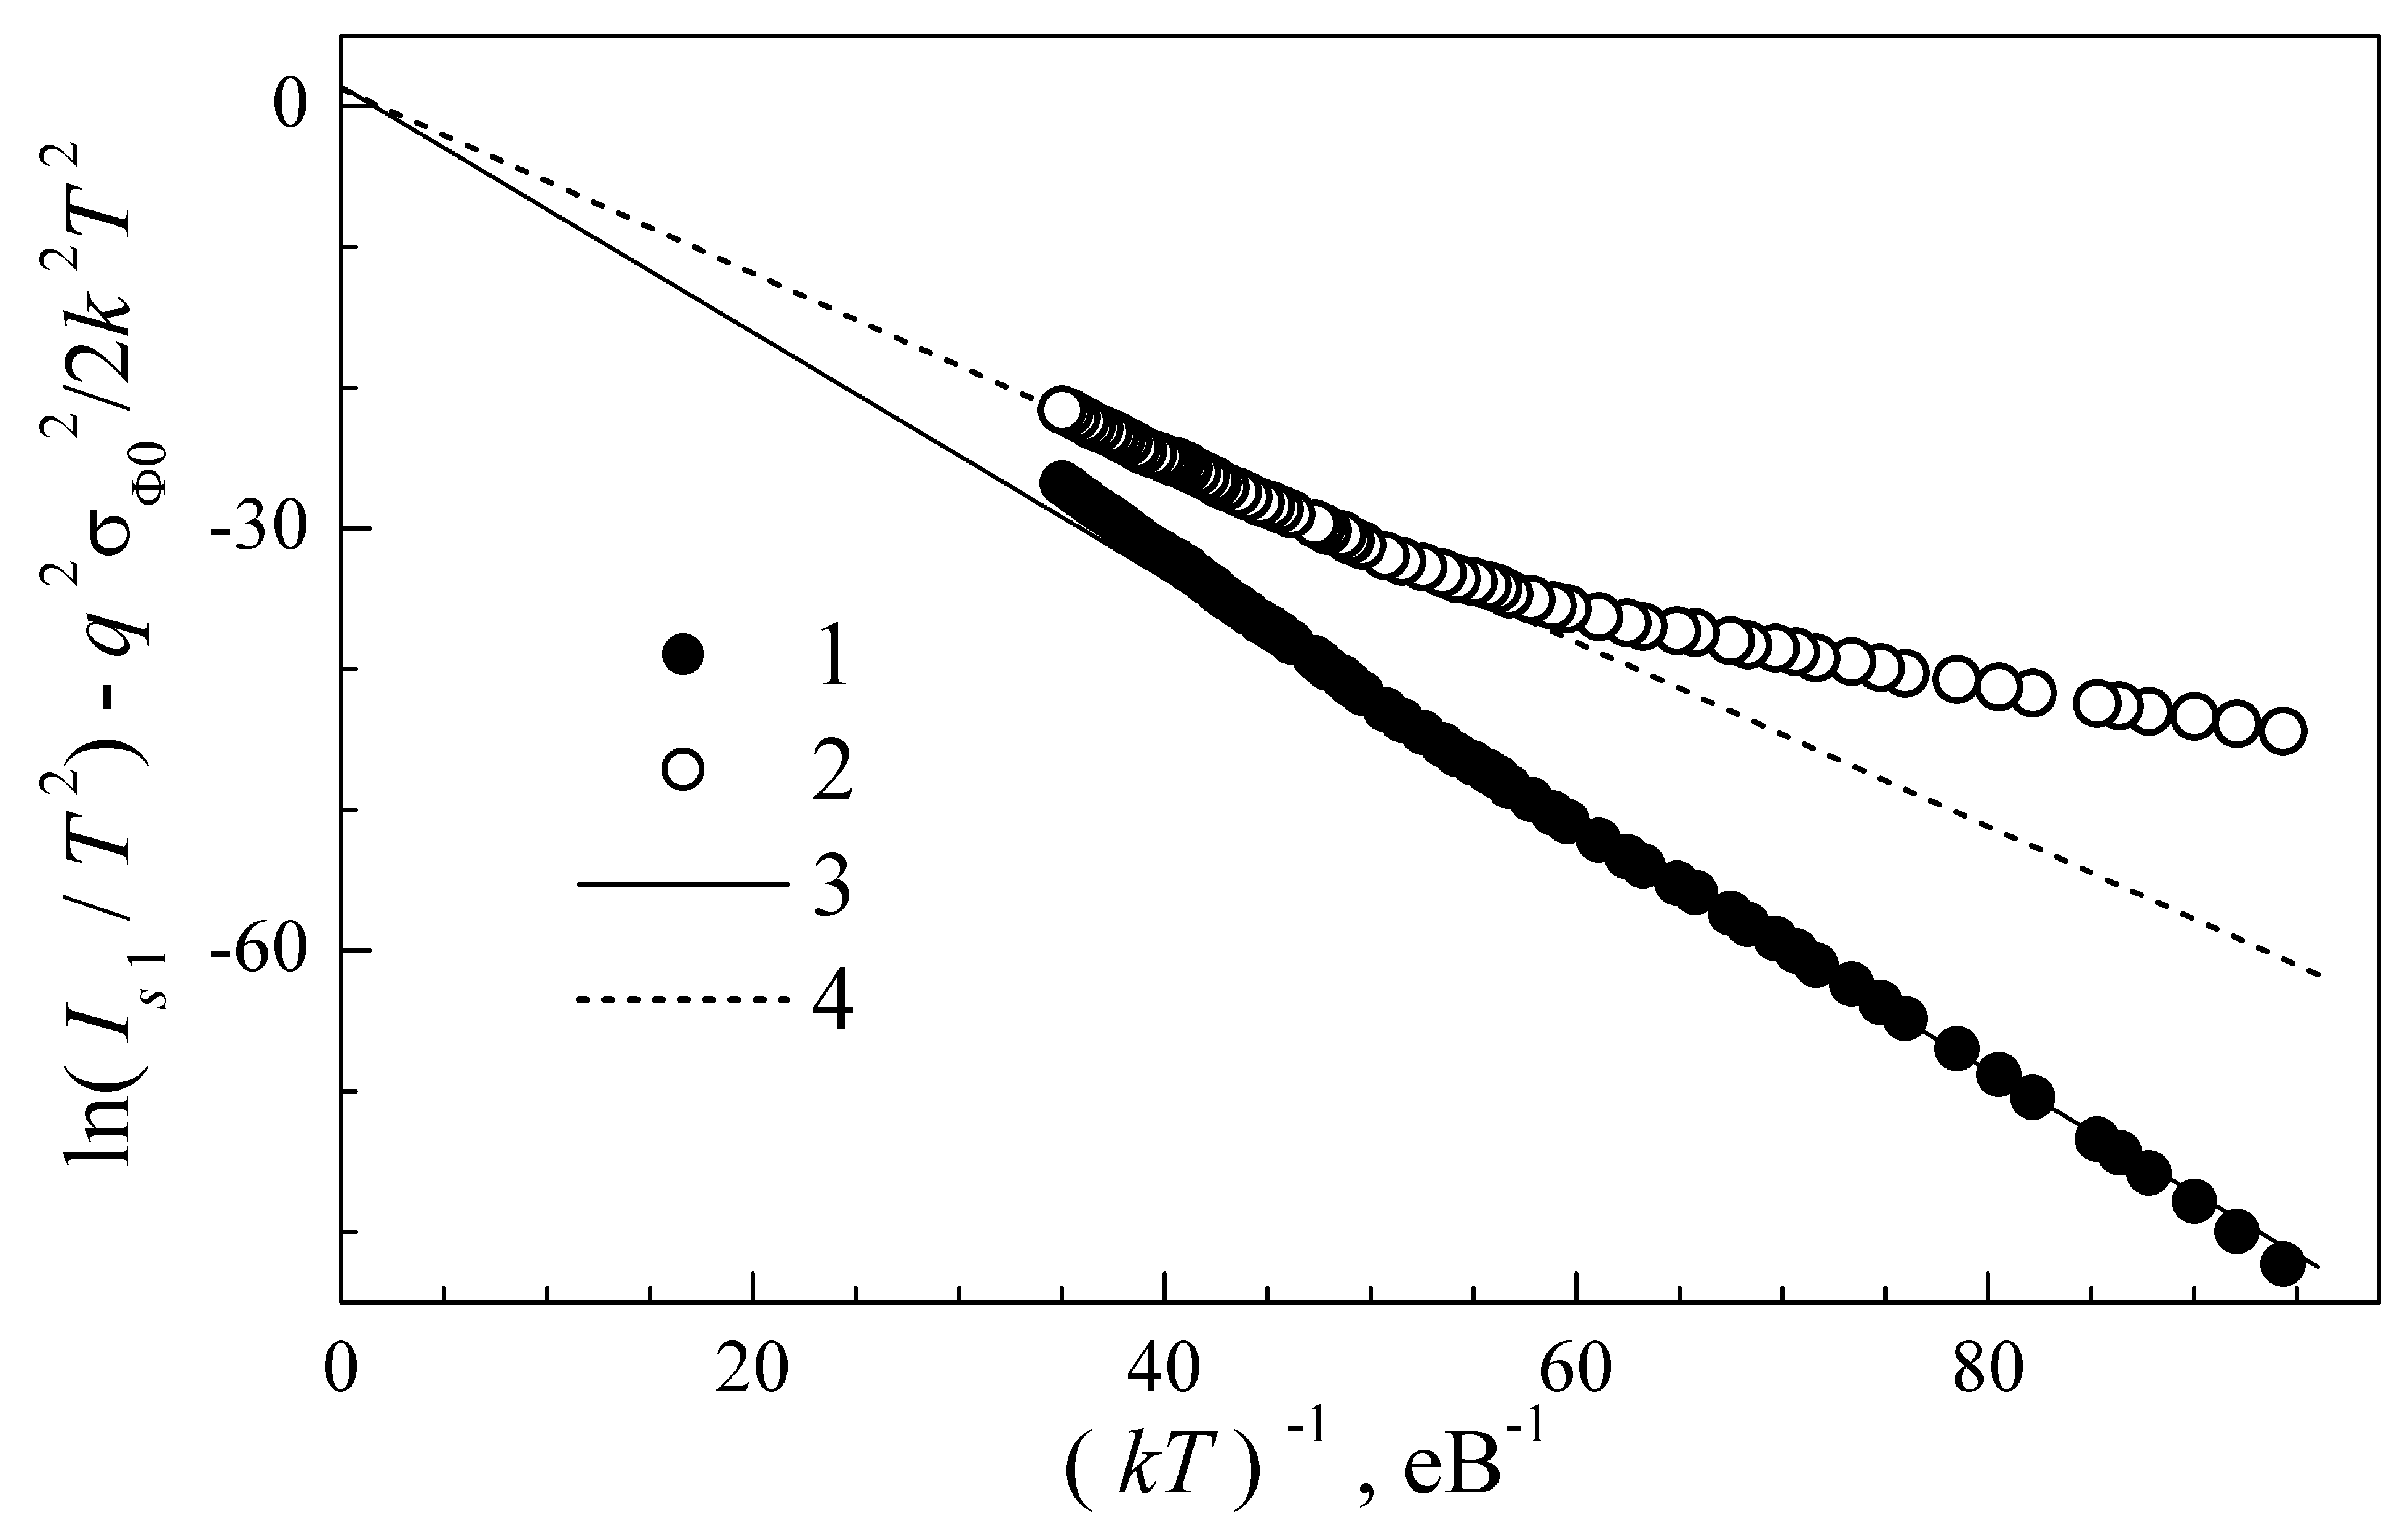
\includegraphics[width=0.7\textwidth]{figRichM_SDA}
\caption{\label{figRichM_SDA}
Модифіковані залежності Річардсона, розраховані за формулою (\ref{eqRich:Mod}) для $I_{s1}$.
$\sigma_{\Phi,0}$, В: 0,099 (крива 1) та 0,04 (2).
Прямі 3 та 4 --- лінійна апроксимація кривих 1 та 2 в діапазонах (130$\div$220)~К
та (230$\div$330)~К, відповідно
}%
\end{figure}

У табл.~\ref{tabPar:SSDA} також наведено значення висоти бар'єру, визначене з ВФХ.
У цьому випадку  \cite{Rhoderick1988,Schroder2006}:
\begin{equation}\label{eqFbCV}
\Phi_{b,CV}=V_n+V_0+kT/q,
\end{equation}
де
$V_0$ --- абсциса точки перетину з віссю напруг прямої, яка апроксимує залежність $1/C^2=f(V)$ (рис.~\ref{figCV}).
Зазначимо, що визначена таким способом ВБШ має перевищувати величину, отриману за допомогою ВАХ
\cite{Rhoderick1988,GELCZUK2014,Mohan,Cetin2005,Soylu,Yildirim2010,Karatas:2006NIMA}.
Це зумовлено тим, що $\Phi_{b,CV}$ визначається, насамперед, вигином зон і на неї не впливають
сили зображення чи квантово--механічне тунелювання носіїв \cite{Rhoderick1988,GELCZUK2014,Mohan}.
Більше того, неоднорідність контакту також не відображається на величині $\Phi_{b,CV}$ на відміну від ВБШ,
яка визначається за допомогою ВАХ \cite{Sullivan,Tung:PhysRev,GELCZUK2014,Mohan}.
За своєю поведінкою зі зміною температури $\Phi_{b,CV}$ нагадує ВБШ, визначену за умов плоских зон, наближаючись
до неї і за величиною \cite{Cetin2005,Soylu,Yildirim2010,Mohan}.
У нашому випадку спостерігається очікуване співвідношення $\Phi_{b,CV}>\Phi_b^0$ для всіх значень, отриманих
У наближенні неоднорідного контакту.

Отже, наведені результати свідчать, що струм $I_1$ може бути описаний в рамках моделі ТЕ через неоднорідний бар'єр.
Єдине, що потребує детальнішої уваги --- відмінність між значеннями $\Phi_b^0$ та  $\sigma_{\Phi0}$ в різних температурних діапазонах,
яка безпосередньо не передбачається в рамках теорії неоднорідного контакту.
Водночас подібна ситуація нерідко спостерігається експериментально, див., наприклад,
\cite{Tascioglu2010old,Yildirim2010,Mamor,Jiang:DGJap,JYOTHI2015,DURMUS2014,KHURE2015,OZAVCI2013,Tung:ApplPhysRev}.
Причиною вважалося домінування при низьких температурах інших, порівняно з ТЕ, механізмів перенесення заряду
(термопольової емісія, тунелювання чи рекомбінаційних процесів), фазові перетворення в металі тощо.
Проте, на думку автора, для досліджених структур збіг  отриманих значень $A^*$ із літературними свідчить про застосовність саме теорії ТЕ у всьому температурному діапазоні.
Причиною зміни нахилів залежностей на рис.~\ref{figFbNT1_SDA} та \ref{figRichM_SDA} може бути збільшення швидкості емісії електронів дефектами на межі МН.
Дійсно, звільнення рівнів окремих дефектів при $T\approx225$~K має стати причиною зменшення ВБШ, а також того,
що частина ділянок неоднорідності, в околі яких концентрація подібних дефектів підвищена, перестане бути зонами полегшеного проходження струму внаслідок ефективного захоплення дрейфуючих електронів пастками.
Як наслідок, у більш високотемпературному діапазоні $\sigma_{\Phi0}$ має зменшуватися, що і спостерігається на експерименті.
Інший варіант пояснення, який пропонується, зокрема, в роботі \cite{Tung:ApplPhysRev},
полягає в тому, що окрім патчів наявна додаткова неоднорідність інтерфейсу метал---напівпровідник.
Зазвичай із ВАХ вдається визначити ВБШ для ділянок із меншим значенням $\Phi_b^0$ і лише при низькотемпературних вимірюваннях
нахил модифікованої залежності Річардсона дозволяє отримати інформацію про верхню межу розподілу висоти бар'єру.


Повертаючись до струму $I_2$, який превалює при малих зміщеннях у низькотемпературній області, зазначимо наступне.
У роботі~\cite{Tung:PhysRev} показано, що у випадку неоднорідного контакту такий додатковий, порівняно з $I_1$, струм
може з'являтися саме при низьких температурах внаслідок ефективного проходженню носіїв через патчі.
При цьому експериментальна залежність, показана на рис.~\ref{figIV_SDA} дуже схожа на передбачену теоретично (див. Fig.6 в \cite{Tung:PhysRev}).
Крім того, у теорії очікується, що для відповідної ділянки ВАХ фактор неідеальності має значно перевищувати одиницю
і має спостерігатися суттєвий вплив послідовного опору.
Саме це і виявлене у експерименті.
У випадку, коли струм через патчі визначається ТЕ, то згідно з \cite{Sarpatwari, Tung:PhysRev}
\begin{equation}\label{eqIlowT}
I_s=f_pAA^*T^2\exp\left(-\frac{q\Phi_{b,p}}{kT}\right),
\end{equation}
де
$f_p$  --- множник, який враховує площу ділянок неоднорідності,
$\Phi_{b,p}$ --- ВБШ в області патчу.
Порівнюючи вирази (\ref{eqIlowT}) та (\ref{eqFb:TE}), запишемо:
%можна записати співвідношення між $\Phi_{b,p}$ та $\Phi_{b}$:
\begin{equation}\label{eqFbFbp}
\Phi_b=\Phi_{b,p}-\frac{kT}{q}\ln{f_p}\,.
\end{equation}
Як видно з рис.~\ref{figFbT_SDA}, величина $\Phi_{b2}$ дійсно є лінійною функцією температури.
Шляхом лінійної апроксимації експериментальних даних визначено, що $\Phi_{b,p}=(54\pm4)$~мВ,
$f_p=(8\pm1)\cdot10^{-13}$.
Отже, додатковий струм, який виникає при низьких температурах, також може бути пояснений з погляду моделі неоднорідного контакту Шотткі.

\subsection{Зворотне зміщення}
\begin{figure}
\center
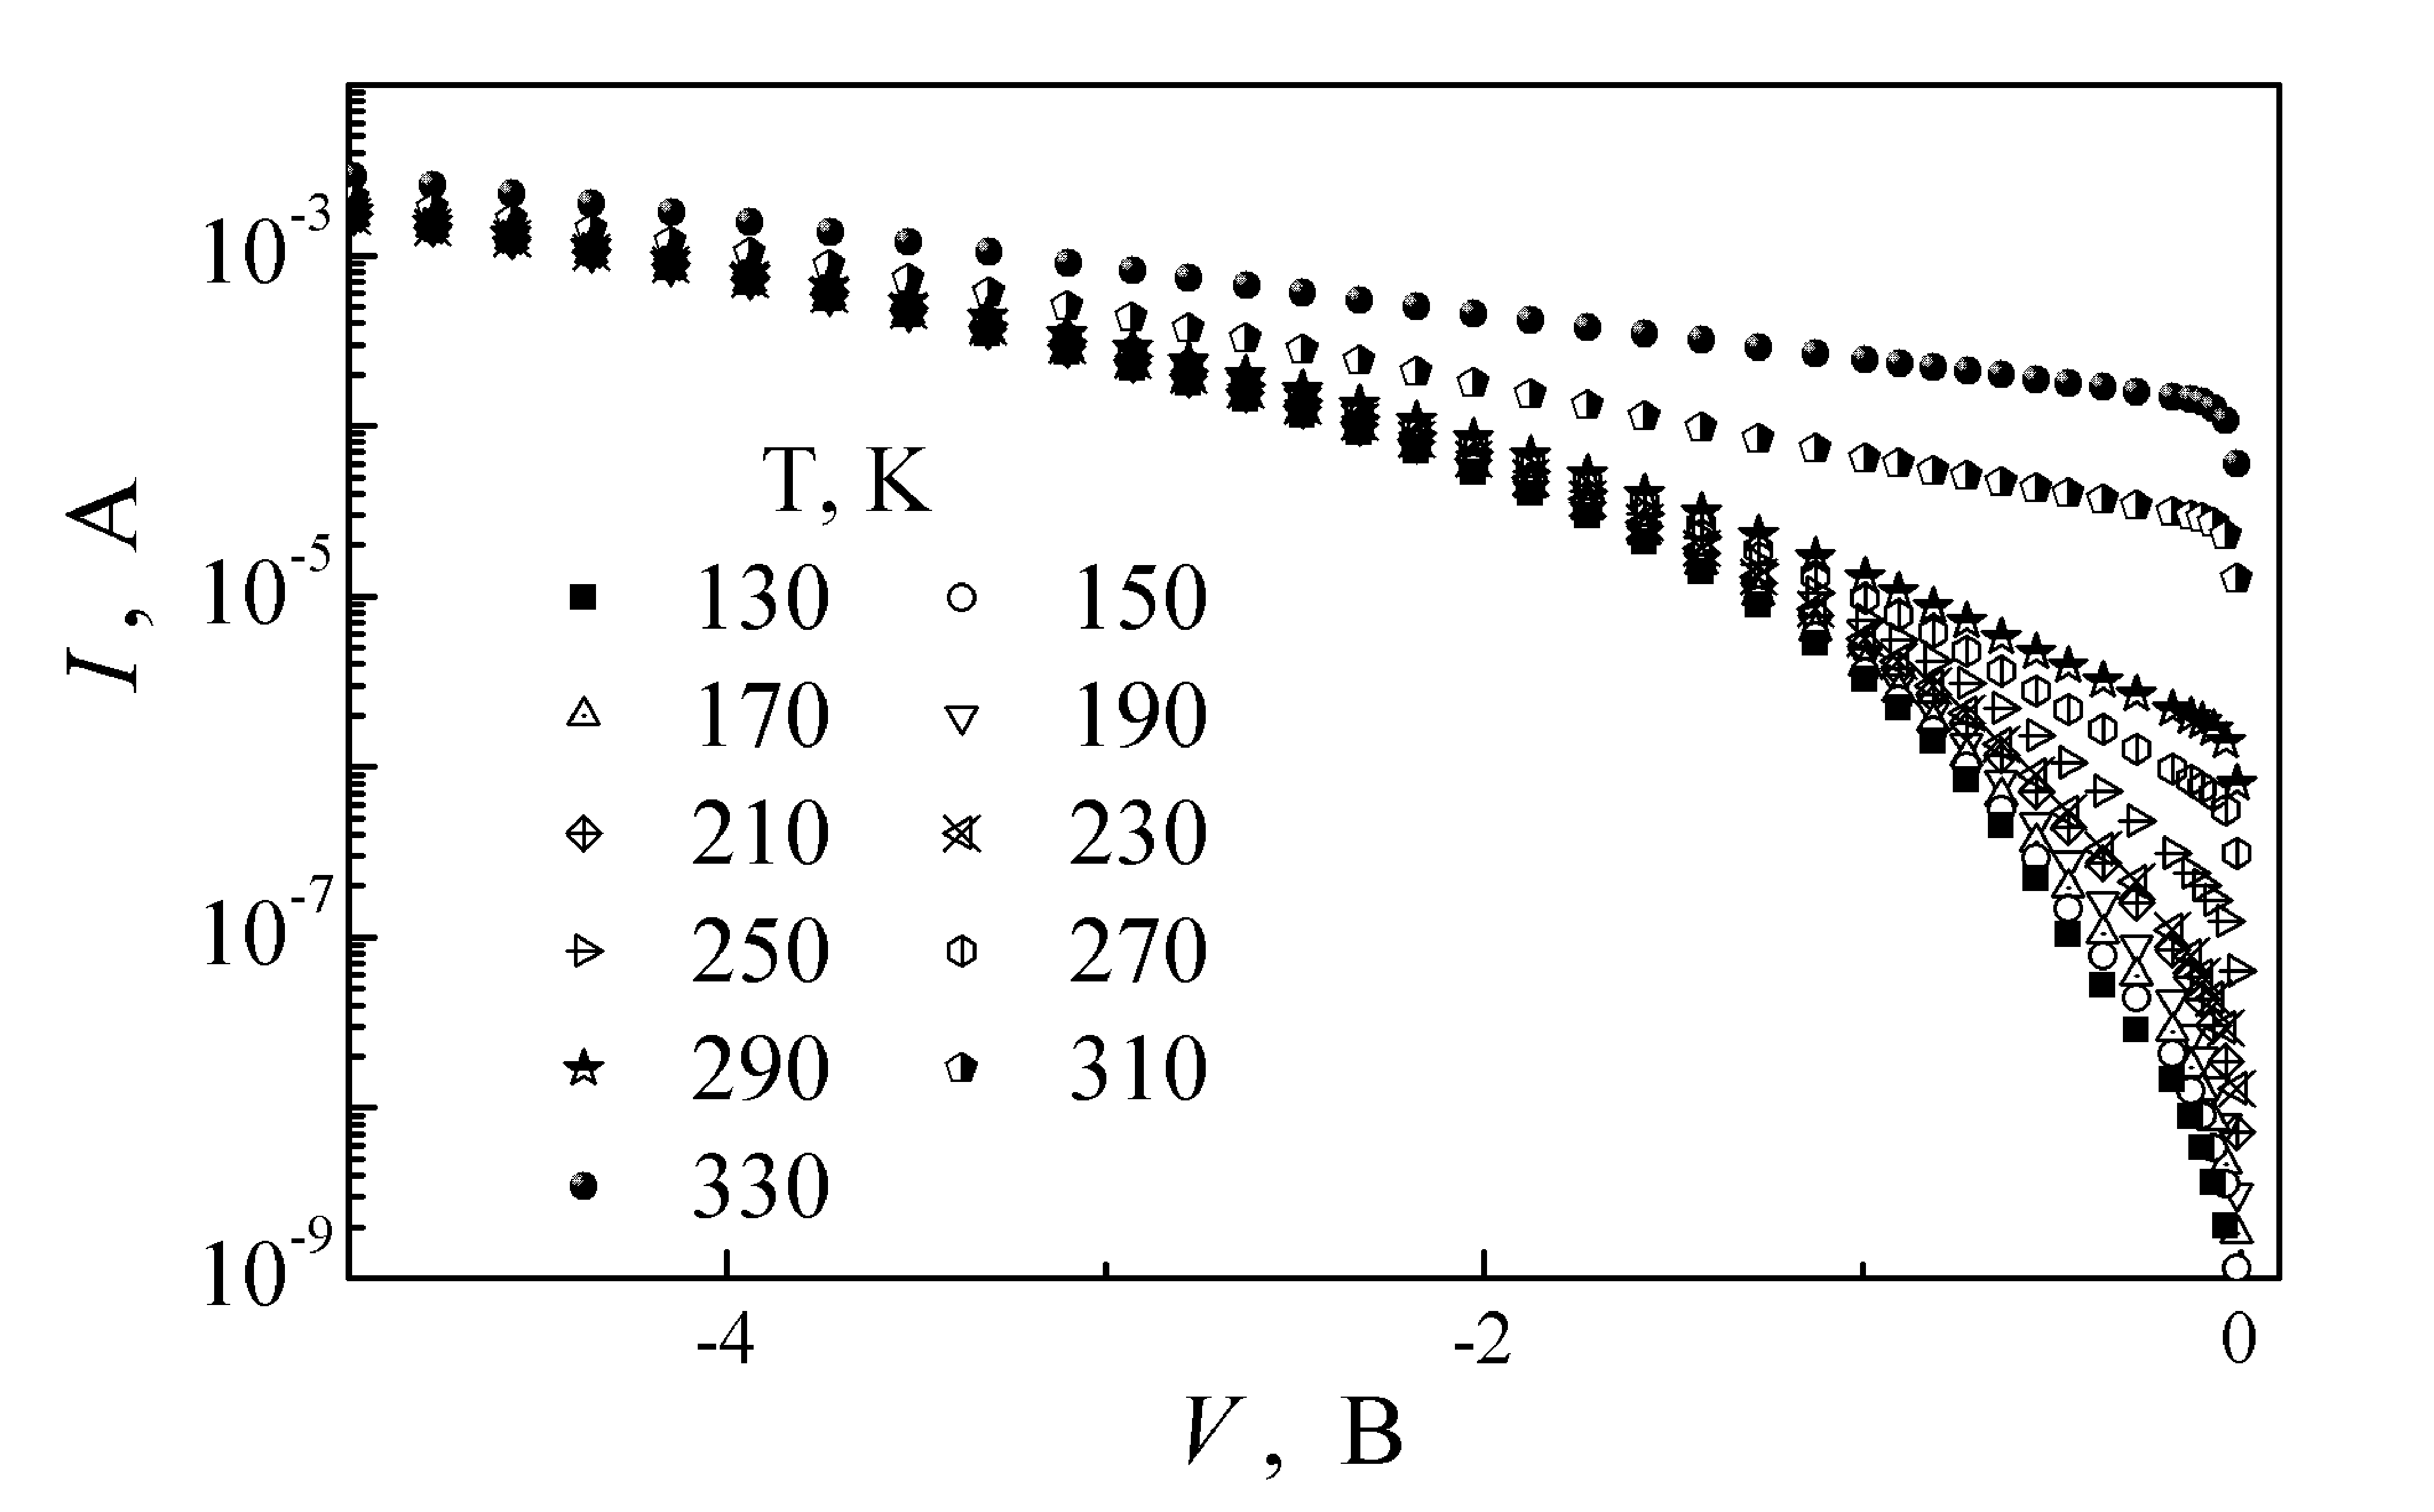
\includegraphics[width=0.65\textwidth]{figIV_SDAr}
\caption{\label{figIV_SDAr}
Зворотні ділянки ВАХ структур SSDA в температурному діапазоні 130$\div$330~K.
Наведено криві, виміряні з кроком 20~К.
}%
\end{figure}

\begin{figure}[b]
\center
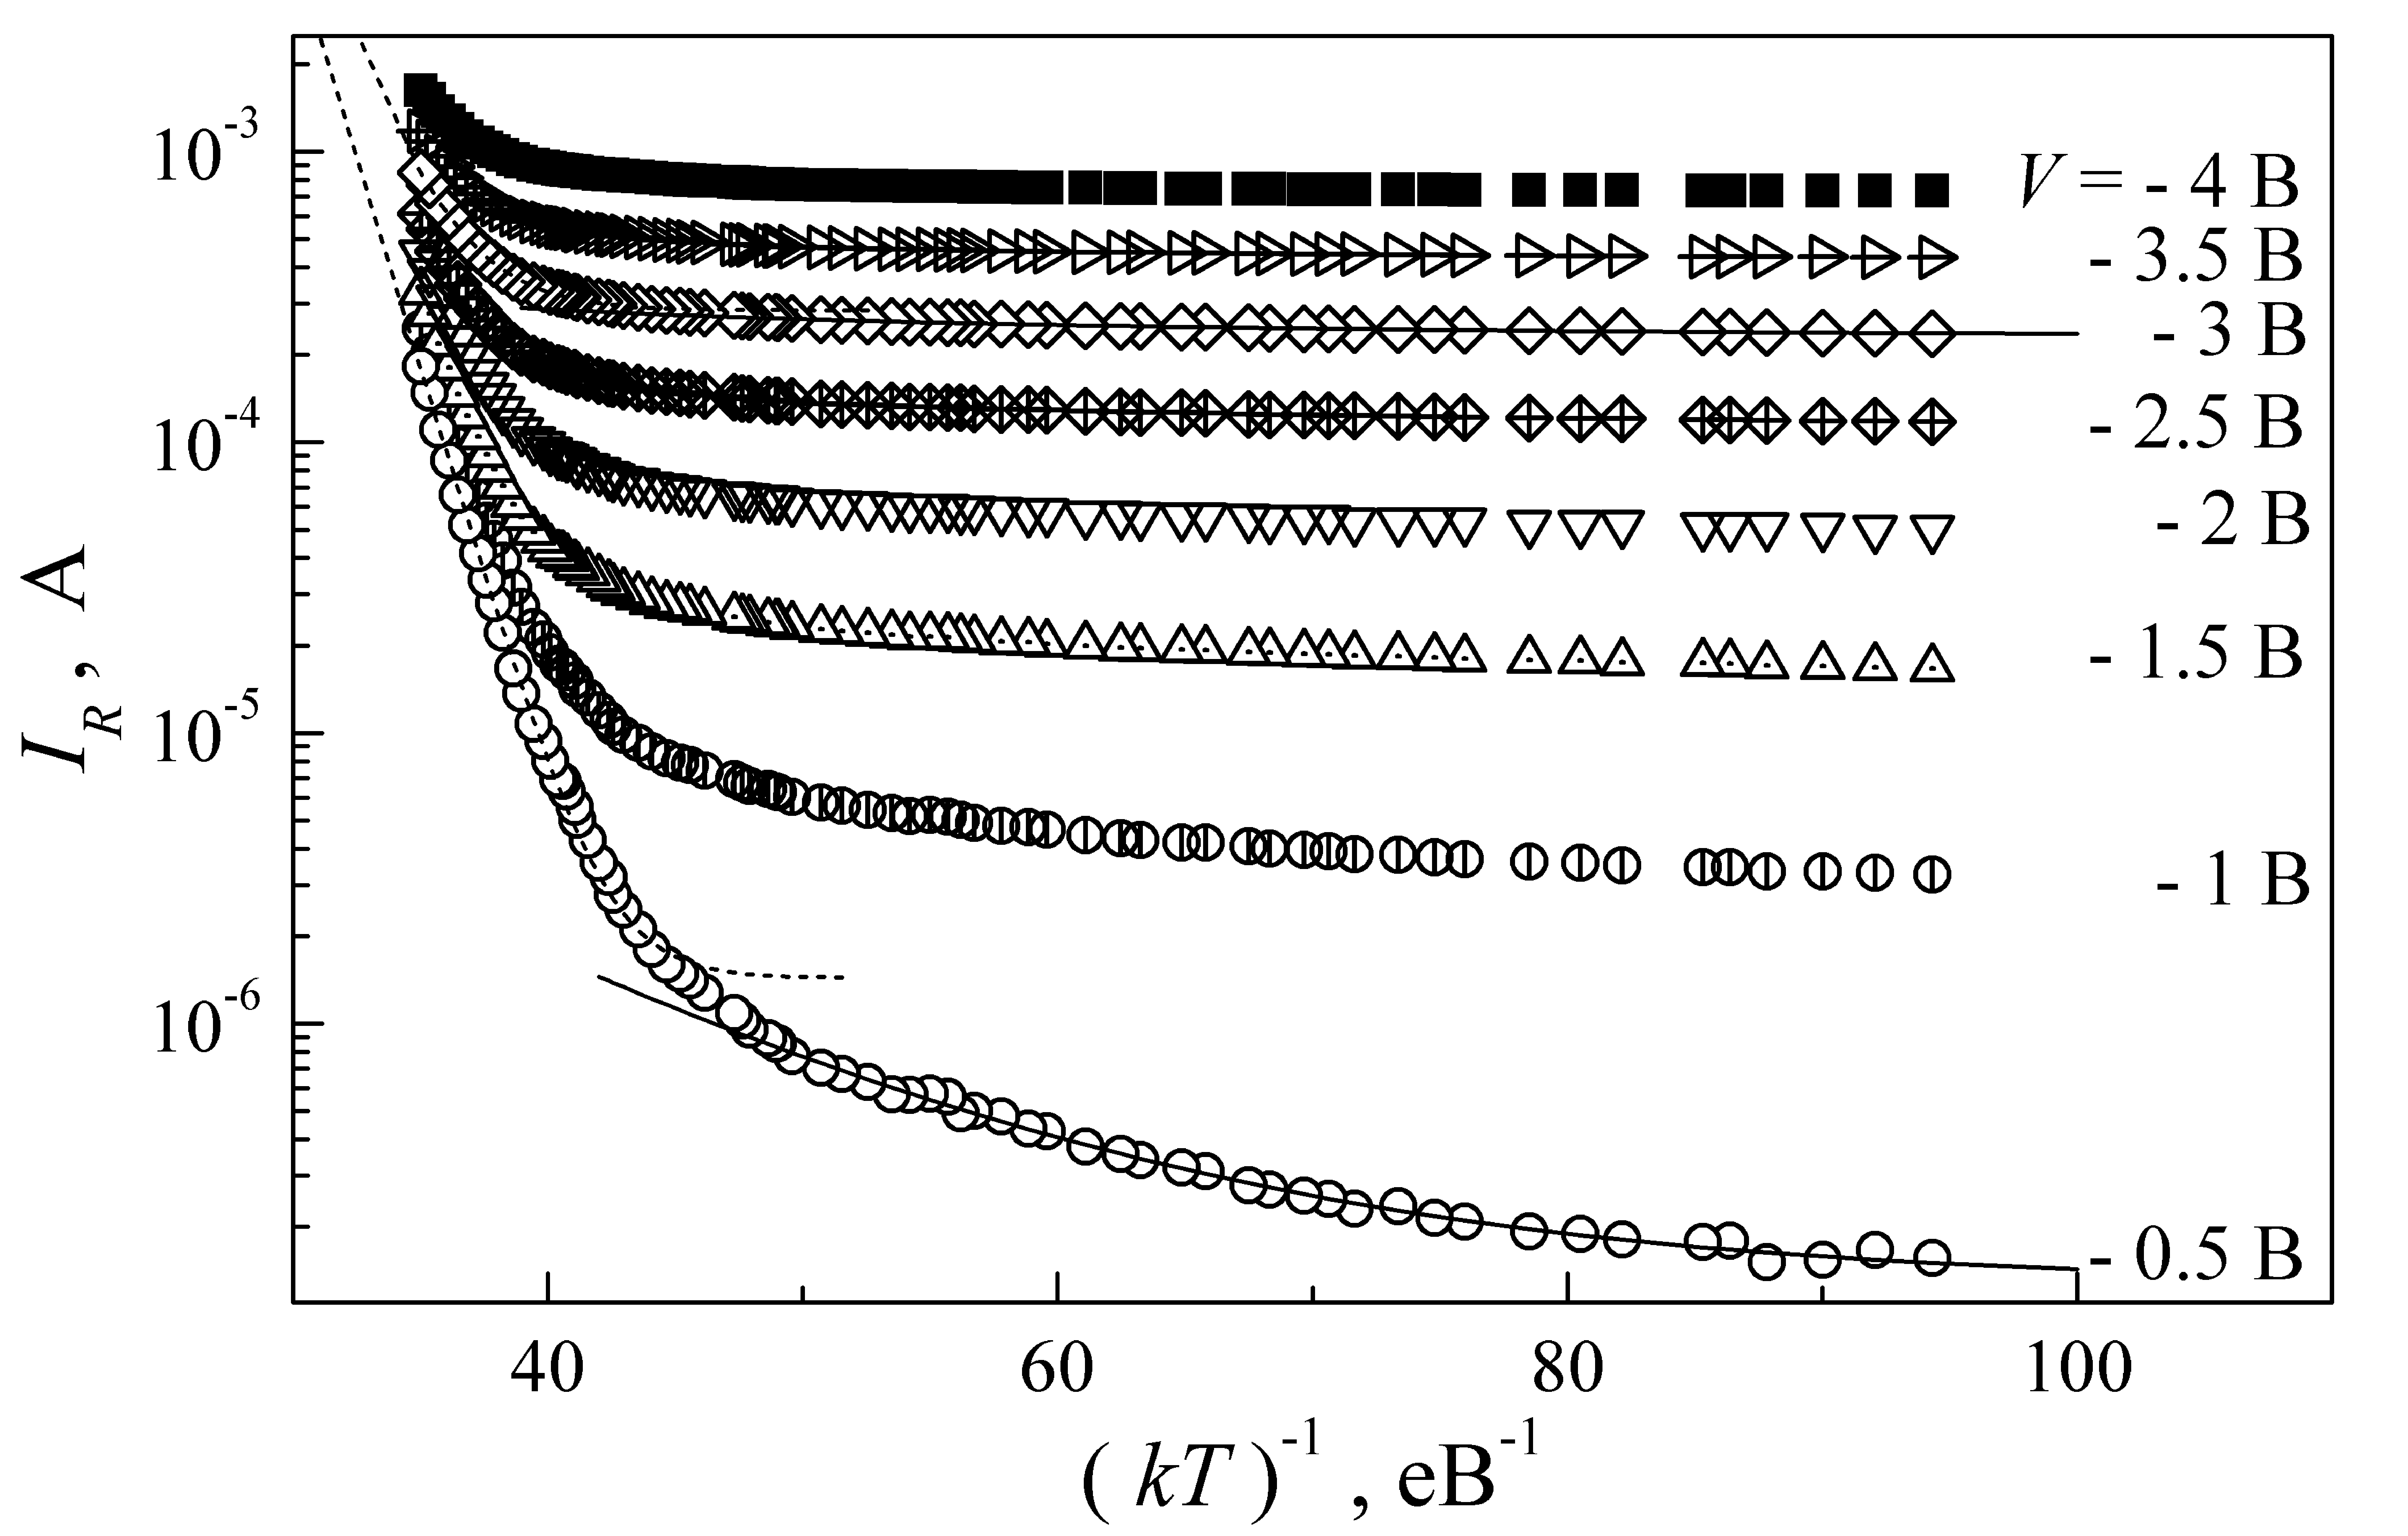
\includegraphics[width=0.65\textwidth]{figIT_SDAr}
\caption{\label{figIT_SDAr}
Температурна залежність зворотного струму структур SSDA при різних зміщеннях.
Точки --- експеримент, лінії --- апроксимація згідно з (\ref{eqIr})
(суцільні при (130$\div$220)~К, пунктирні при (230$\div$330)~К).
}%
\end{figure}

Приклади зворотних гілок ВАХ структур SSDA, виміряних при різних температурах, наведено на рис.~\ref{figIV_SDAr}.
На представлених характеристиках не спостерігається насичення величини зворотного струму $I_R$.
Це свідчить,
що характеристики не можуть бути описані в рамках моделі ТЕ через бар'єр із постійною для певної температури висотою.
Зауважимо, що подібна поведінка (відсутність насичення зворотного струму) є типовою
практично для всіх реальних ДШ.
Це явище навіть отримало окрему назву --- <<м'які>> (<<soft>>) зворотні характеристики.
Зростання струму при підвищенні температури залежить від зміщення:
при збільшенні зворотної напруги $V_R$ температурна залежність $I_R$ послаблюється.
З метою з'ясування механізму перенесення заряду були побудовані залежності величини струму при певному значенні напруги від температури,
представлені на рис.~\ref{figIT_SDAr}.
З рисунка видно, що
\begin{enumerate}[label=\asbuk*),leftmargin=0em,itemindent=1.5em]
\item при аналізі зворотних ВАХ також, як і для прямих гілок, доцільно розглядати два температурних піддіапазони (130$\div$220)~К та (230$\div$330)~К;
\item при зворотному зміщенні існує декілька механізмів перенесення заряду.
\end{enumerate}








Проведений аналіз показав, що польова та температурна залежність зворотного струму можуть бути описані
за допомогою виразу
\begin{eqnarray}
\label{eqIr}
\nonumber I_R(T,V_R)&=&I_\mathrm{TE}(T,V_R)+I_\mathrm{FN}(V_R)=\\
&=&C_\mathrm{TE}(V_R)T^2\exp\left[-\frac{E_\mathrm{TE}(V_R)}{kT}\right]+I_\mathrm{FN}(V_R)\,,
\end{eqnarray}
де перший доданок $I_\mathrm{TE}$ описує ТЕ компоненту струму, яка залежить від температури та напруги,
а другий $I_\mathrm{FN}$ --- температурно-незалежну;
величини  $C_\mathrm{TE}$ та $E_\mathrm{TE}$ також не залежать від температури.

\label{nu_IR}
Для оцінки внеску кожної з компонент використані величини
\begin{equation*}
 \nu_\mathrm{TE}=\frac{I_\mathrm{TE}}{I_R}=\frac{I_\mathrm{TE}}{I_\mathrm{TE}+I_\mathrm{FN}}\,,\qquad
 \nu_\mathrm{FN}=\frac{I_\mathrm{FN}}{I_R}=\frac{I_\mathrm{FN}}{I_\mathrm{TE}+I_\mathrm{FN}}\,.
\end{equation*}
Температурна та польова залежності $\nu_\mathrm{TE}$ та $\nu_\mathrm{FN}$ показані на рис.~\ref{figeIr_SDA}.
Внесок ТЕ складової зростає при підвищенні температури та зменшенні зворотної напруги, проте характер
залежностей суттєво залежить від конкретних значень $T$ та $V_R$.


\begin{figure}
\center
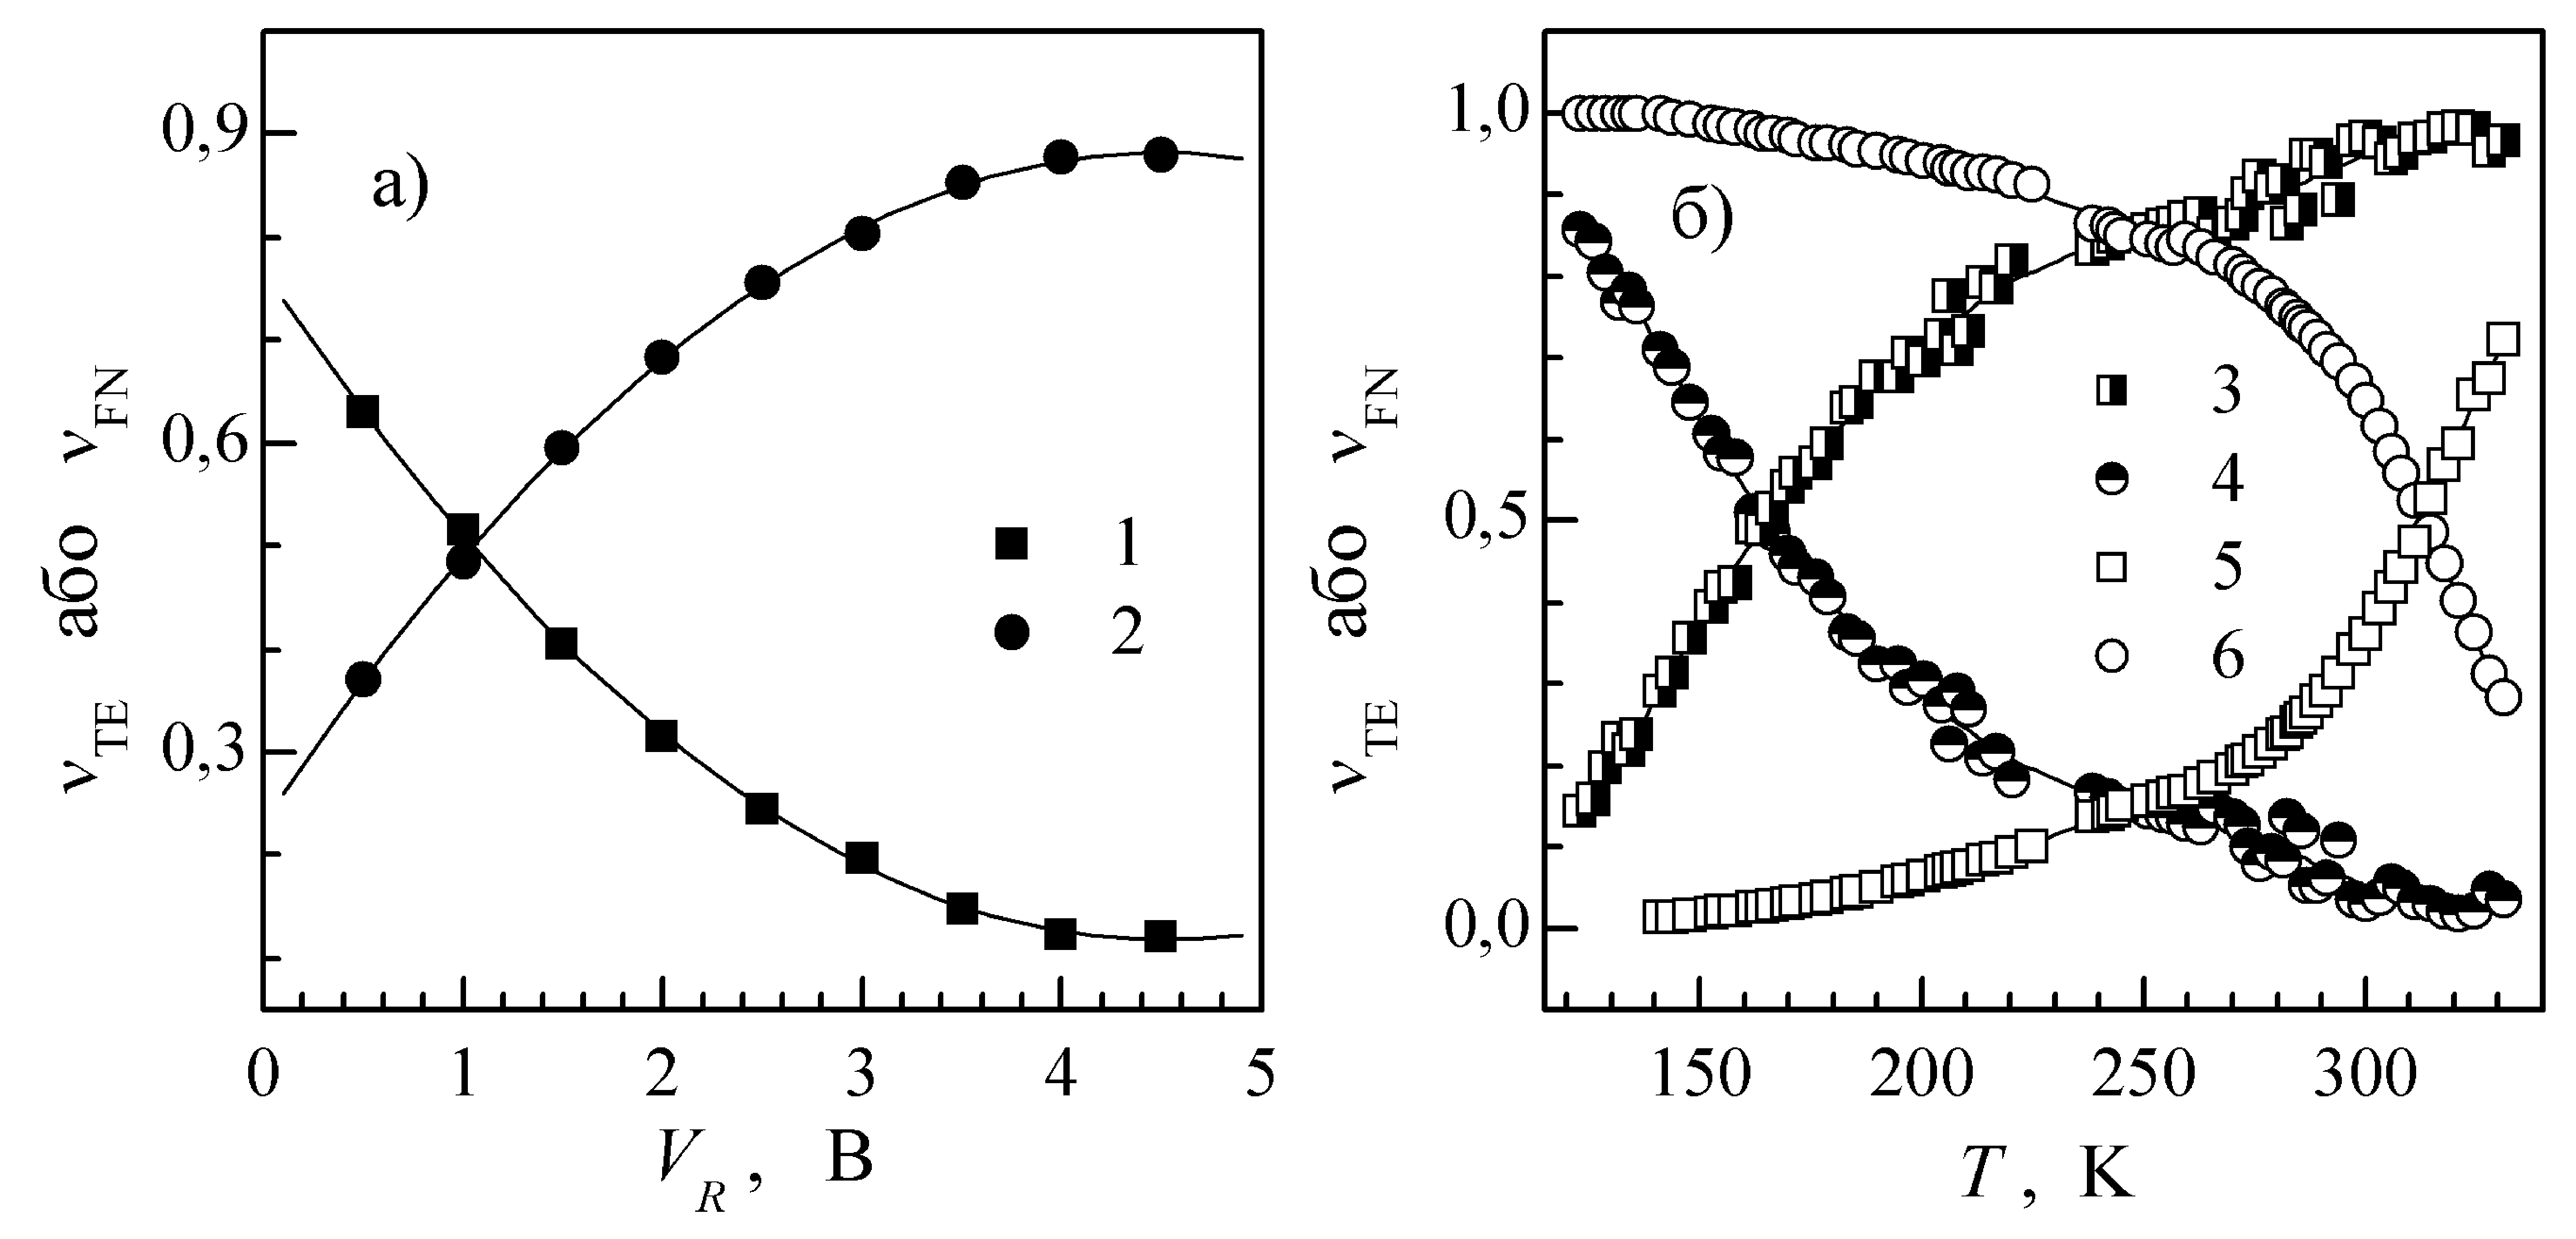
\includegraphics[width=0.9\textwidth]{figeIr_SDA}
\caption{\label{figeIr_SDA}
Залежність відносного внеску у зворотний струм
ТЕ (криві 1, 3 та 5) та температуро--незалежної (криві 2, 4 та 6)
компонент від зміщення при $T=300$~К (а) та
від температури (б) при $V_R=0,5$~В (3 та 4) і $V_R=3$~В (5 та 6)
}%
\end{figure}

Виявлена залежність характеристичної енергії $E_\mathrm{TE}$ від прикладеної напруги є свідченням зміни ВБШ.
Відомо \cite{Rhoderick1988,Tung:PhysRev,Andrews}, що зменшення висоти бар'єру при зворотному зміщенні може відбуватися під дією сил зображення
(при цьому  зміна ВБШ $\Delta\Phi_b\sim V_{bb}^{1/4}$),
електричного поля ($\Delta\Phi_b\sim V_{bb}^{1/2}$),
а також завдяки впливу областей неоднорідності.
В останньому випадку за наявності неоднакових патчів $\Delta\Phi_b\sim V_{bb}^{2/3}$, а коефіцієнт пропорційності залежить від параметрів цих локальних ділянок \cite{Tung:PhysRev}.
Для досліджених структур $E_\mathrm{TE}$ набуває різних значень в кожному з температурних піддіапазонів,
проте при збільшенні зворотного зміщення в обох випадках зменшується, лінійно спадаючи зі зростанням $V^{2/3}_R$ (рис.~\ref{figIrTE_SDA}).
Отже, аналіз зворотних ВАХ також підтверджує,
що струм у структурах SSDA описується у рамках теорії неоднорідного контакту з патчами,
вплив яких змінюється поблизу температури 225~К.



\begin{figure}[b]
\center
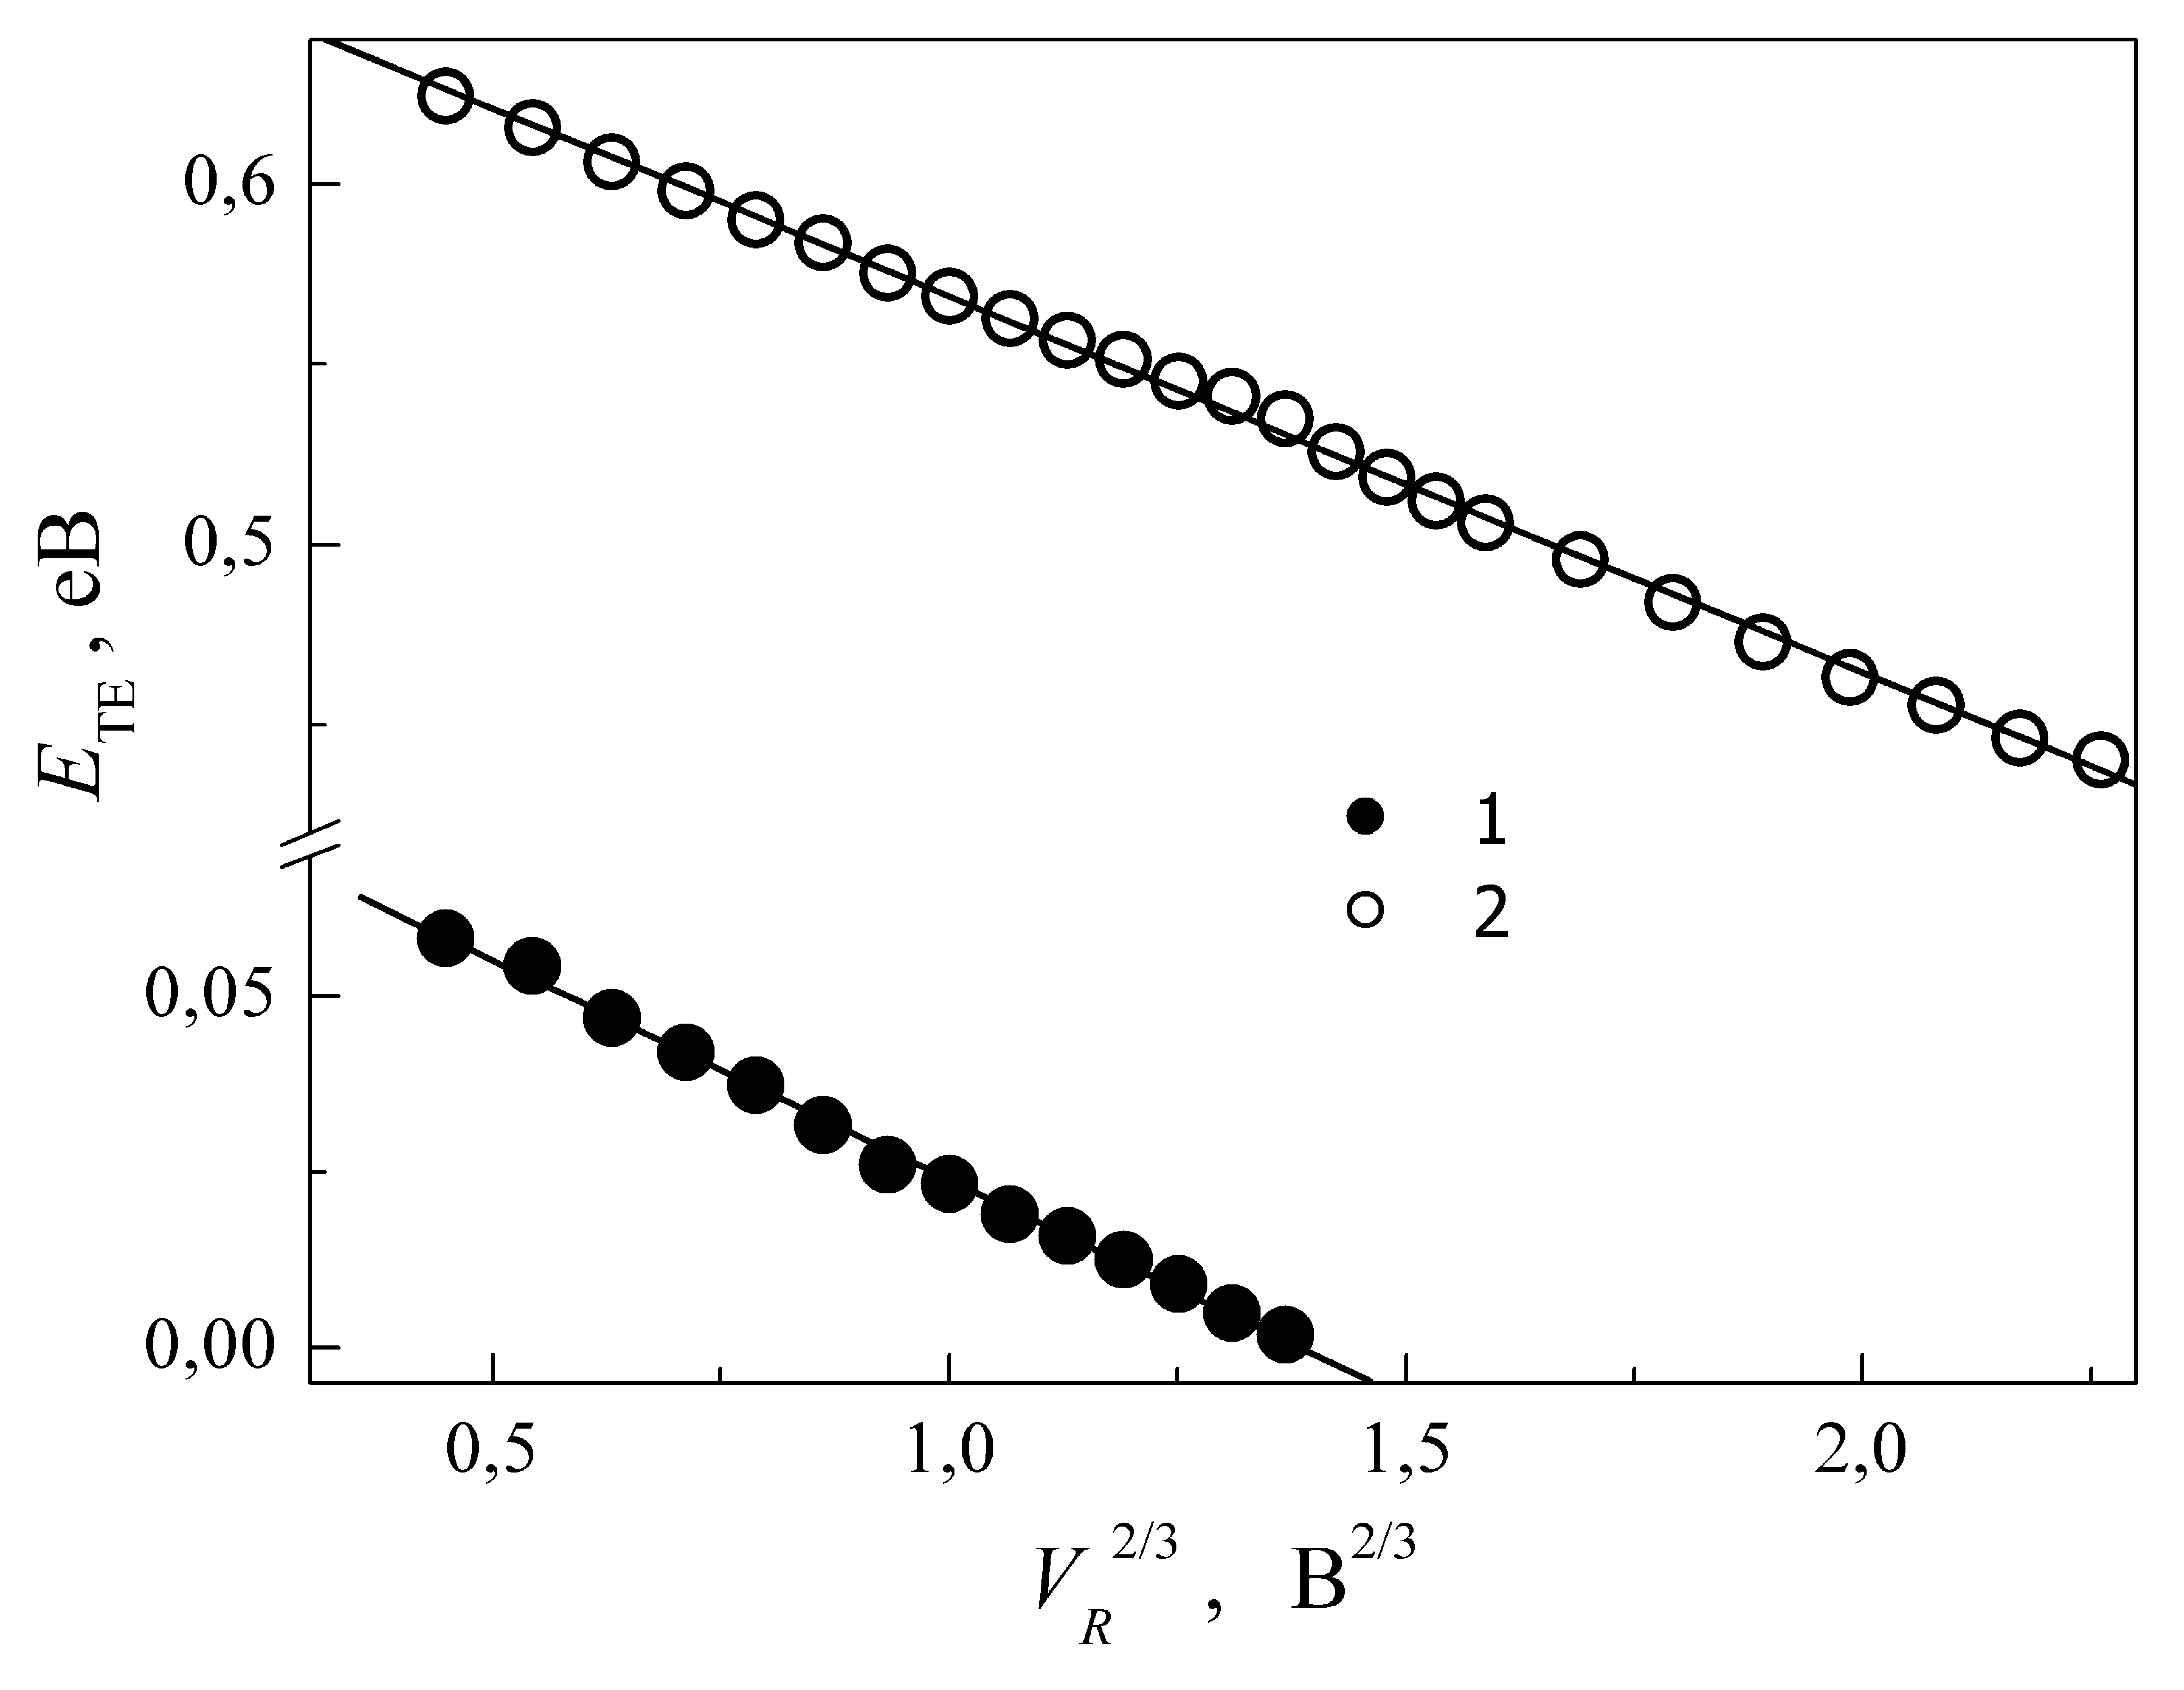
\includegraphics[width=0.55\textwidth]{figIrTE_SDA}
\caption{\label{figIrTE_SDA}
Польові залежності характеристичної енергії ТЕ складової зворотного струму
в діапазонах температур  (130$\div$220)~К (крива 1) та   (230$\div$330)~К (крива 2).
Точки --- експеримент, прямі --- лінійна апроксимація %за методом найменших квадратів
}%
\end{figure}

На рис.~\ref{figIrFN_SDA} наведено польові залежності величини струму $I_\mathrm{FN}$ у координатах Фаулера--Нордгейма
$\ln(I_\mathrm{FN}/F_m^2)=f(1/F_M)$,
де
\begin{equation}\label{eqFm}
  F_m=\left(\frac{2qN_{d}V_{bb}}{\varepsilon_s\varepsilon_0}\right)^{1/2}
\end{equation}
напруженість електричного поля на межі метал---напівпровідник \cite{Rhoderick1988};
при розрахунках $F_m$ використовувалися отримані при аналізі прямих ВАХ значення $\Phi^0_b$ та  $V_n$ при $T=250$~К.
Лінійність залежності свідчить про тунельний характер цієї компоненти струму \cite{Evtuh},
що також підтверджується незалежністю величини $I_\mathrm{FN}$ від температури.


\begin{figure}
\center
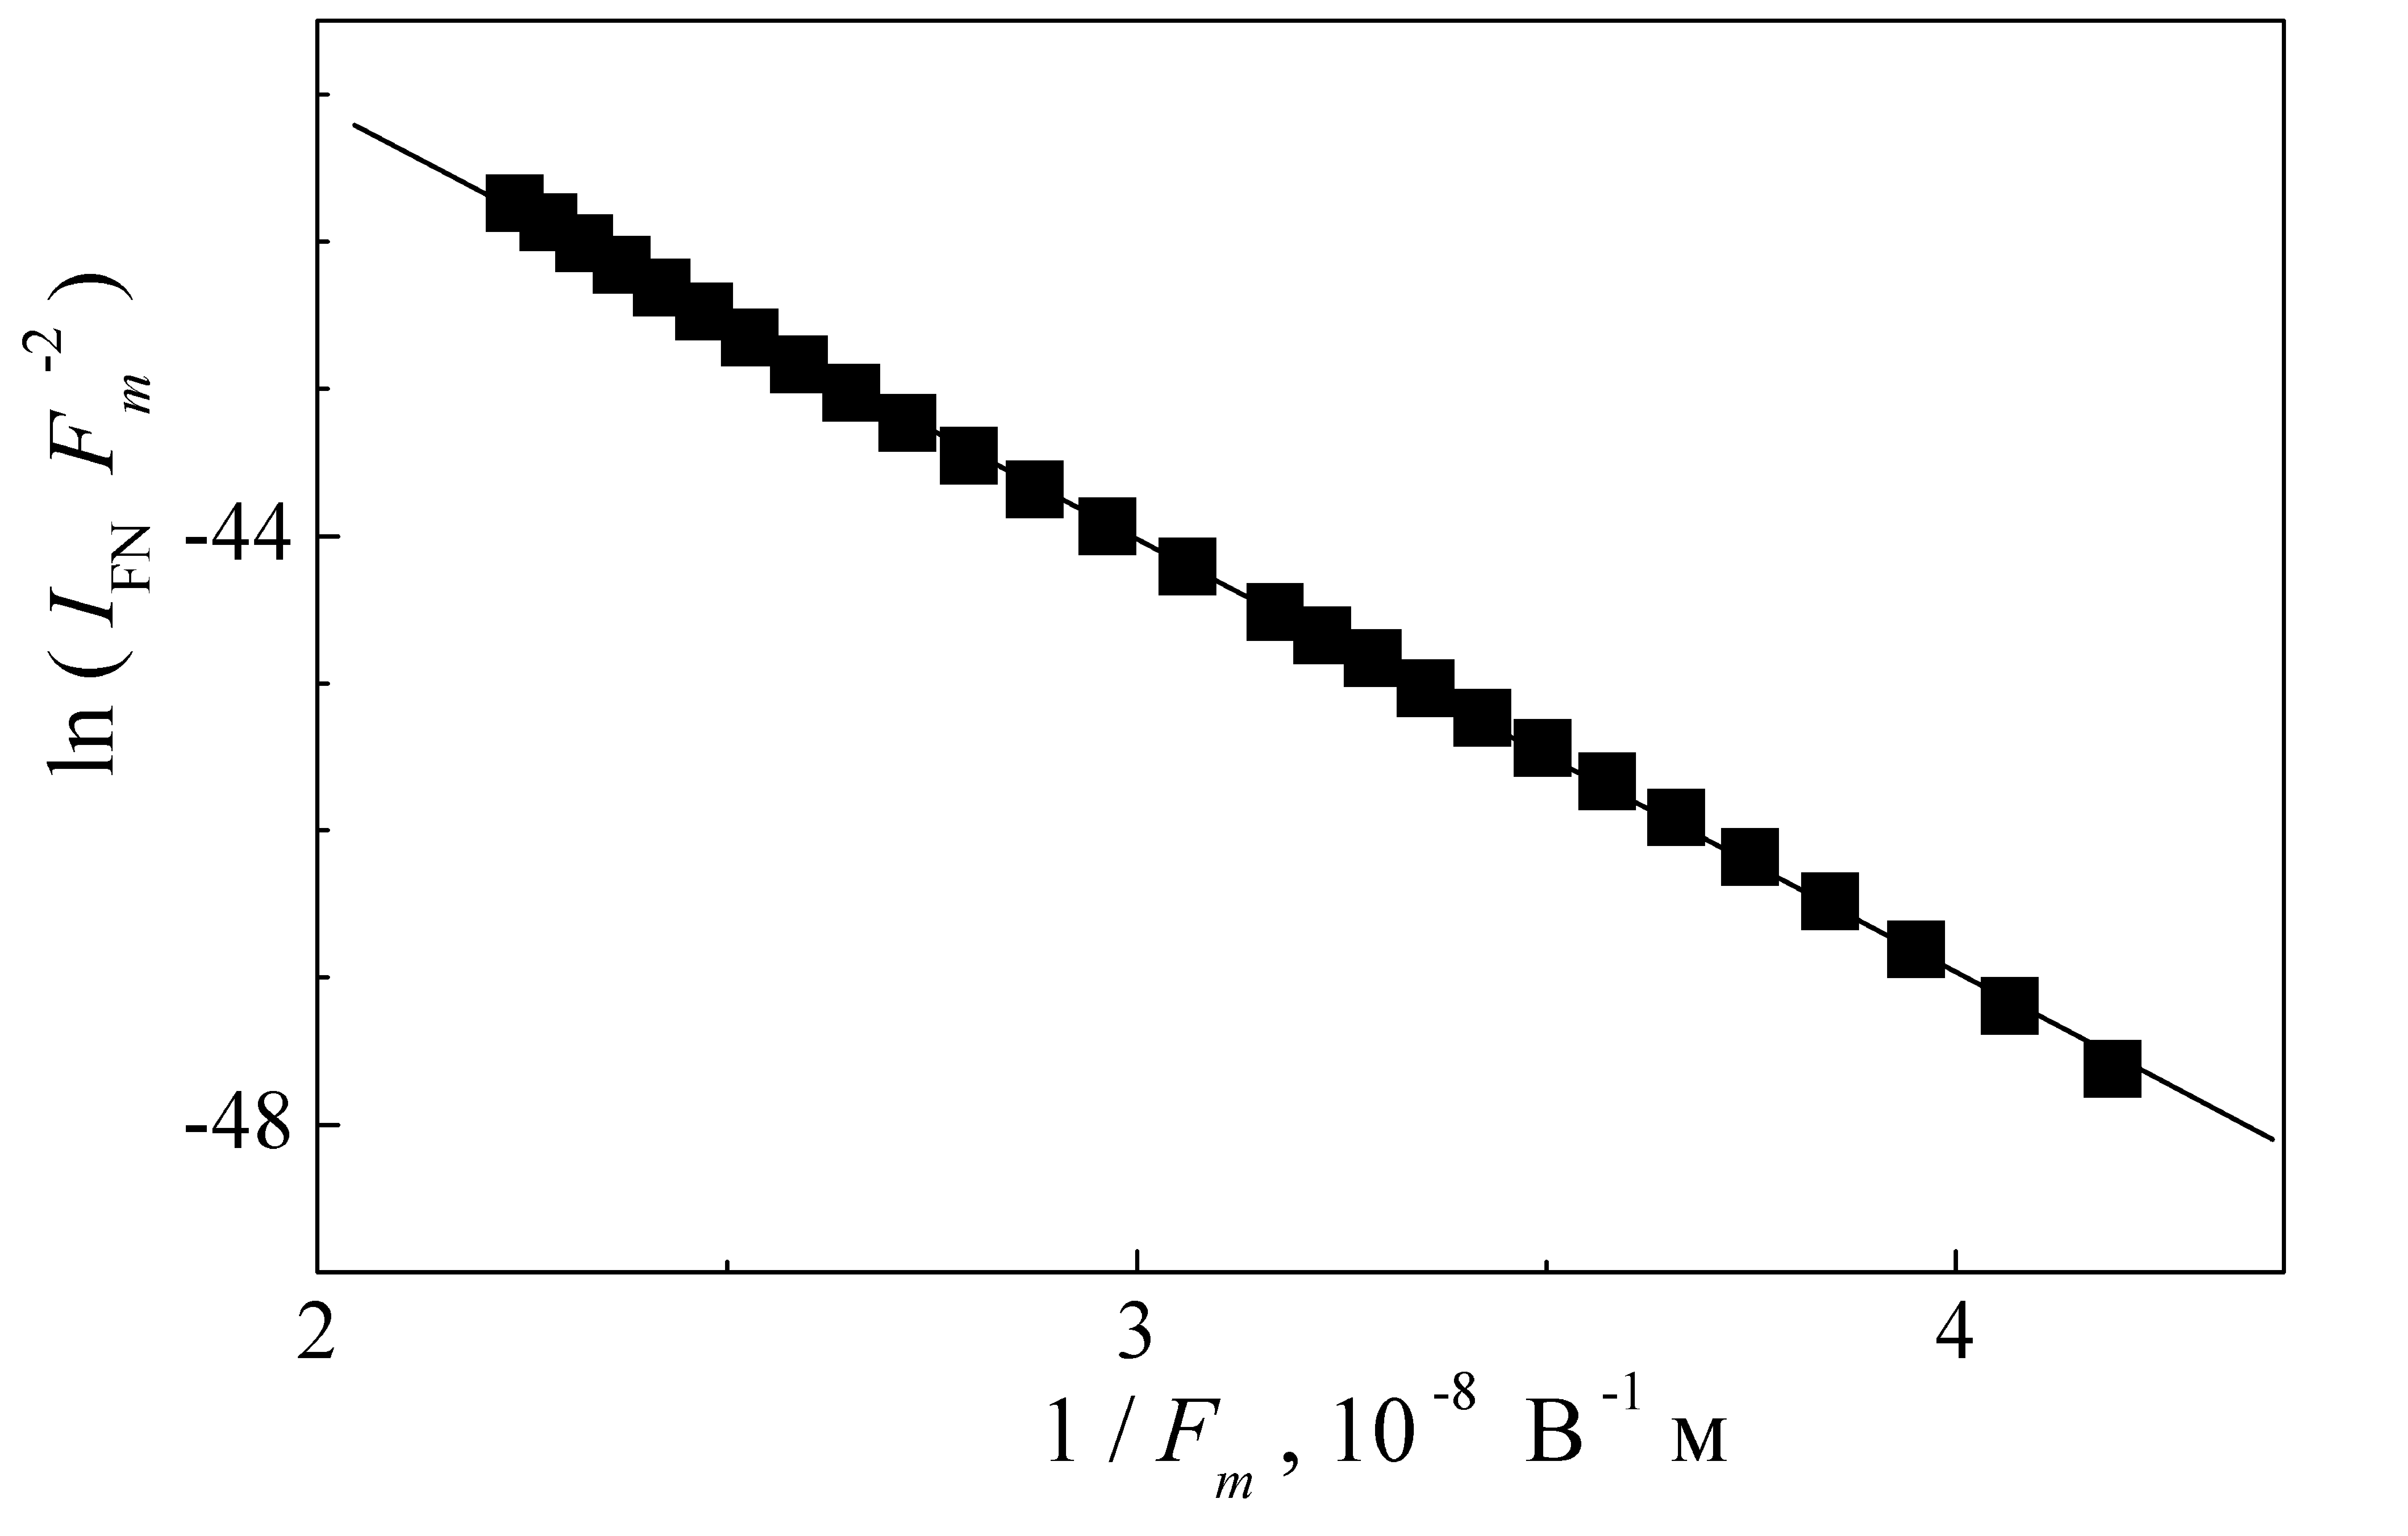
\includegraphics[width=0.6\textwidth]{figIrFN_SDA}
\caption{\label{figIrFN_SDA}
Залежність температуро--незалежної компоненти зворотного струму
в координатах Фаулера--Нордгейма.
Точки --- експеримент, пряма --- лінійна апроксимація за методом найменших квадратів
}%
\end{figure}

У припущенні, що тунелювання відбувається через трикутний бар'єр, для опису струму може бути застосована
модифікована формула Фаулера--Нордгейма  \cite{Rhoderick1988,Novikov,Kurnosova}:
\begin{equation}\label{eqFowlNord}
    \ln\left(\frac{I_\mathrm{FN}}{F_m^2}\right)\propto -\frac{4 \sqrt{2m^*}(qE_{t,\mathrm{eff}})^{3/2}}{3\hbar q F_m}\,,
\end{equation}
де
$m*$ ---  ефективна маса електрону,
для Si $m* = 1,08\cdot9,11\cdot10^{-31}$~кг,
$E_{t,\mathrm{eff}}$ --- ефективна енергія тунелювання,
яка для випадку тунелюванням через центр у забороненій зоні залежить від глибини залягання рівня $\epsilon_t=E_c-E_t$ \cite{Kurnosova,Bulyarskii2001r}:
\begin{equation}\label{eqFN:Et}
    E_{t,\mathrm{eff}}=E_g\left\{\frac{3}{16}\left[\frac{\pi}{2}-
     \arcsin\left(1-\frac{2\epsilon_t}{E_g}\right)\right]-\frac{3}{8}\left(1-\frac{2\epsilon_t}{E_g}\right)
     \sqrt{\frac{\epsilon_t}{E_g}-\left(\frac{\epsilon_t}{E_g}\right)^2}\right\}^{2/3}
\end{equation}


Апроксимуючи отриману залежність (рис.~\ref{figIrFN_SDA}) згідно з (\ref{eqFowlNord}) та використовуючи (\ref{eqFN:Et}),
знайдено, що $E_c-E_t=(120\pm5)$~меВ.
Ця величина добре узгоджується з акцепторним рівнем міжвузлового атому вуглецю С$_i$: $E_c-(0,10\div0,12)$~еВ \cite{Vavilov1990r,Song1987}.
Отже, компонента струму $I_\mathrm{FN}$ зумовлена прямим тунелюванням через глибокий центр, яким, імовірно, є міжвузловий атом вуглецю.

\section{$\gamma$--індуковані ефекти в структурах Al---$n$--$n^+$--Si\label{MSSi_Rad}}
Частина структур, використаних для досліджень, опромінена $\gamma$--квантами $^{60}$Co.
Як вже згадувалося, на дослідження впливу опромінення на параметри ДШ звертається значна увага.
Зокрема, достовірно виявлено \cite{Kumar1, Rao, Kumar2, Sharma, Ohyama}, що іонне та електронне опромінення ДШ,
створених на основі напівпровідників із електронною провідністю, викликає
монотонні (з підвищенням дози) зменшення висоти бар'єру і зростання фактора неідеальності та зворотного струму.
Ці ефекти виникають внаслідок утворення радіаційних дефектів, які спричинюють зміну концентрації вільних носіїв та
збільшення густини станів на інтерфейсній межі, що, в свою чергу, є причиною підсилення тунельного струму.
Водночас, у структурах із контактом Шотткі, уражених внаслідок дії $\gamma$--квантів, незалежно від матеріалу чи типу провідності,
нерідко спостерігається збільшення ВБШ та зменшення фактора неідеальності \cite{Tataroglu,Tascioglu2010old,Tataroglu:2007NIMA}.
Для пояснення цього явища запропоновано \cite{Tataroglu:2007NIMA} механізм, який передбачає
часткову компенсацію напівпровідника та інтенсифікацію процесів інтерфейсного тунелювання за участю рівнів дефектів (DAT, defect--assisted tunneling).
Проте, у літературі також зустрічаються повідомлення щодо зменшення ВБШ внаслідок $\gamma$--опромінення \cite{Tataroglu3}.
Більше того, якщо визначення ВБШ проводиться за допомогою ВАХ, то зі збільшенням поглинутої дози $\gamma$--квантів $^{60}$Co спостерігаються
і немонотонні зміни висоти бар'єру \cite{Karatas:2006NIMA,Umana,Verma}.
До речі, про дозову немонотонність зміни електричних параметрів повідомляється не лише при $\gamma$--опроміненні ДШ,
але й у випадку інших бар'єрних структур \cite{Kinoshita} та/або типів радіаційного впливу \cite{Vorobets, Pattabi, Kovalyuk}.
Нарешті, варто зауважити, що виявлені немонотонності впливу опромінення на структури МН також бувають різного типу:
наприклад, в роботах \cite{Karatas:2006NIMA, Vorobets, Pattabi} виявлено, що ВБШ збільшується
при малих дозах і зростає при великих (немонотонність типу <<зростання--спад>>), тоді як автори робіт \cite{Umana,Verma} описують протилежну тенденцію (<<спад--зростання>>).
Причини подібних розходжень до цього часу не знайшли належного пояснення.

У роботі доза $\gamma$--опромінення структур SSDA складала $10^6$ або $10^7$~рад, для позначення відповідних зразків, як і в розділі~\ref{Ch_SSC}, використовуються префікси <<g6>> та <<g7>>, відповідно.
При виборі дози  використані результати роботи \cite{Karatas:2006NIMA}, де показано,
що ВБШ кремнієвих структур зростає, якщо загальна поглинута доза $\gamma$--квантів $^{60}$Co $\approx10$~кГр, тоді як при подальшому збільшенні
$D$ до $100$~кГр висота бар'єру зменшується (немонотонність типу <<зростання--спад>>).
Водночас використані дози не викликають значних порушень кристалічної ґратки,
про що, зокрема, свідчить, відсутність впливу $\gamma$--опромінення на концентрацію вільних носіїв заряду --- див. рис.~\ref{figCVrad}

\begin{figure}
\center
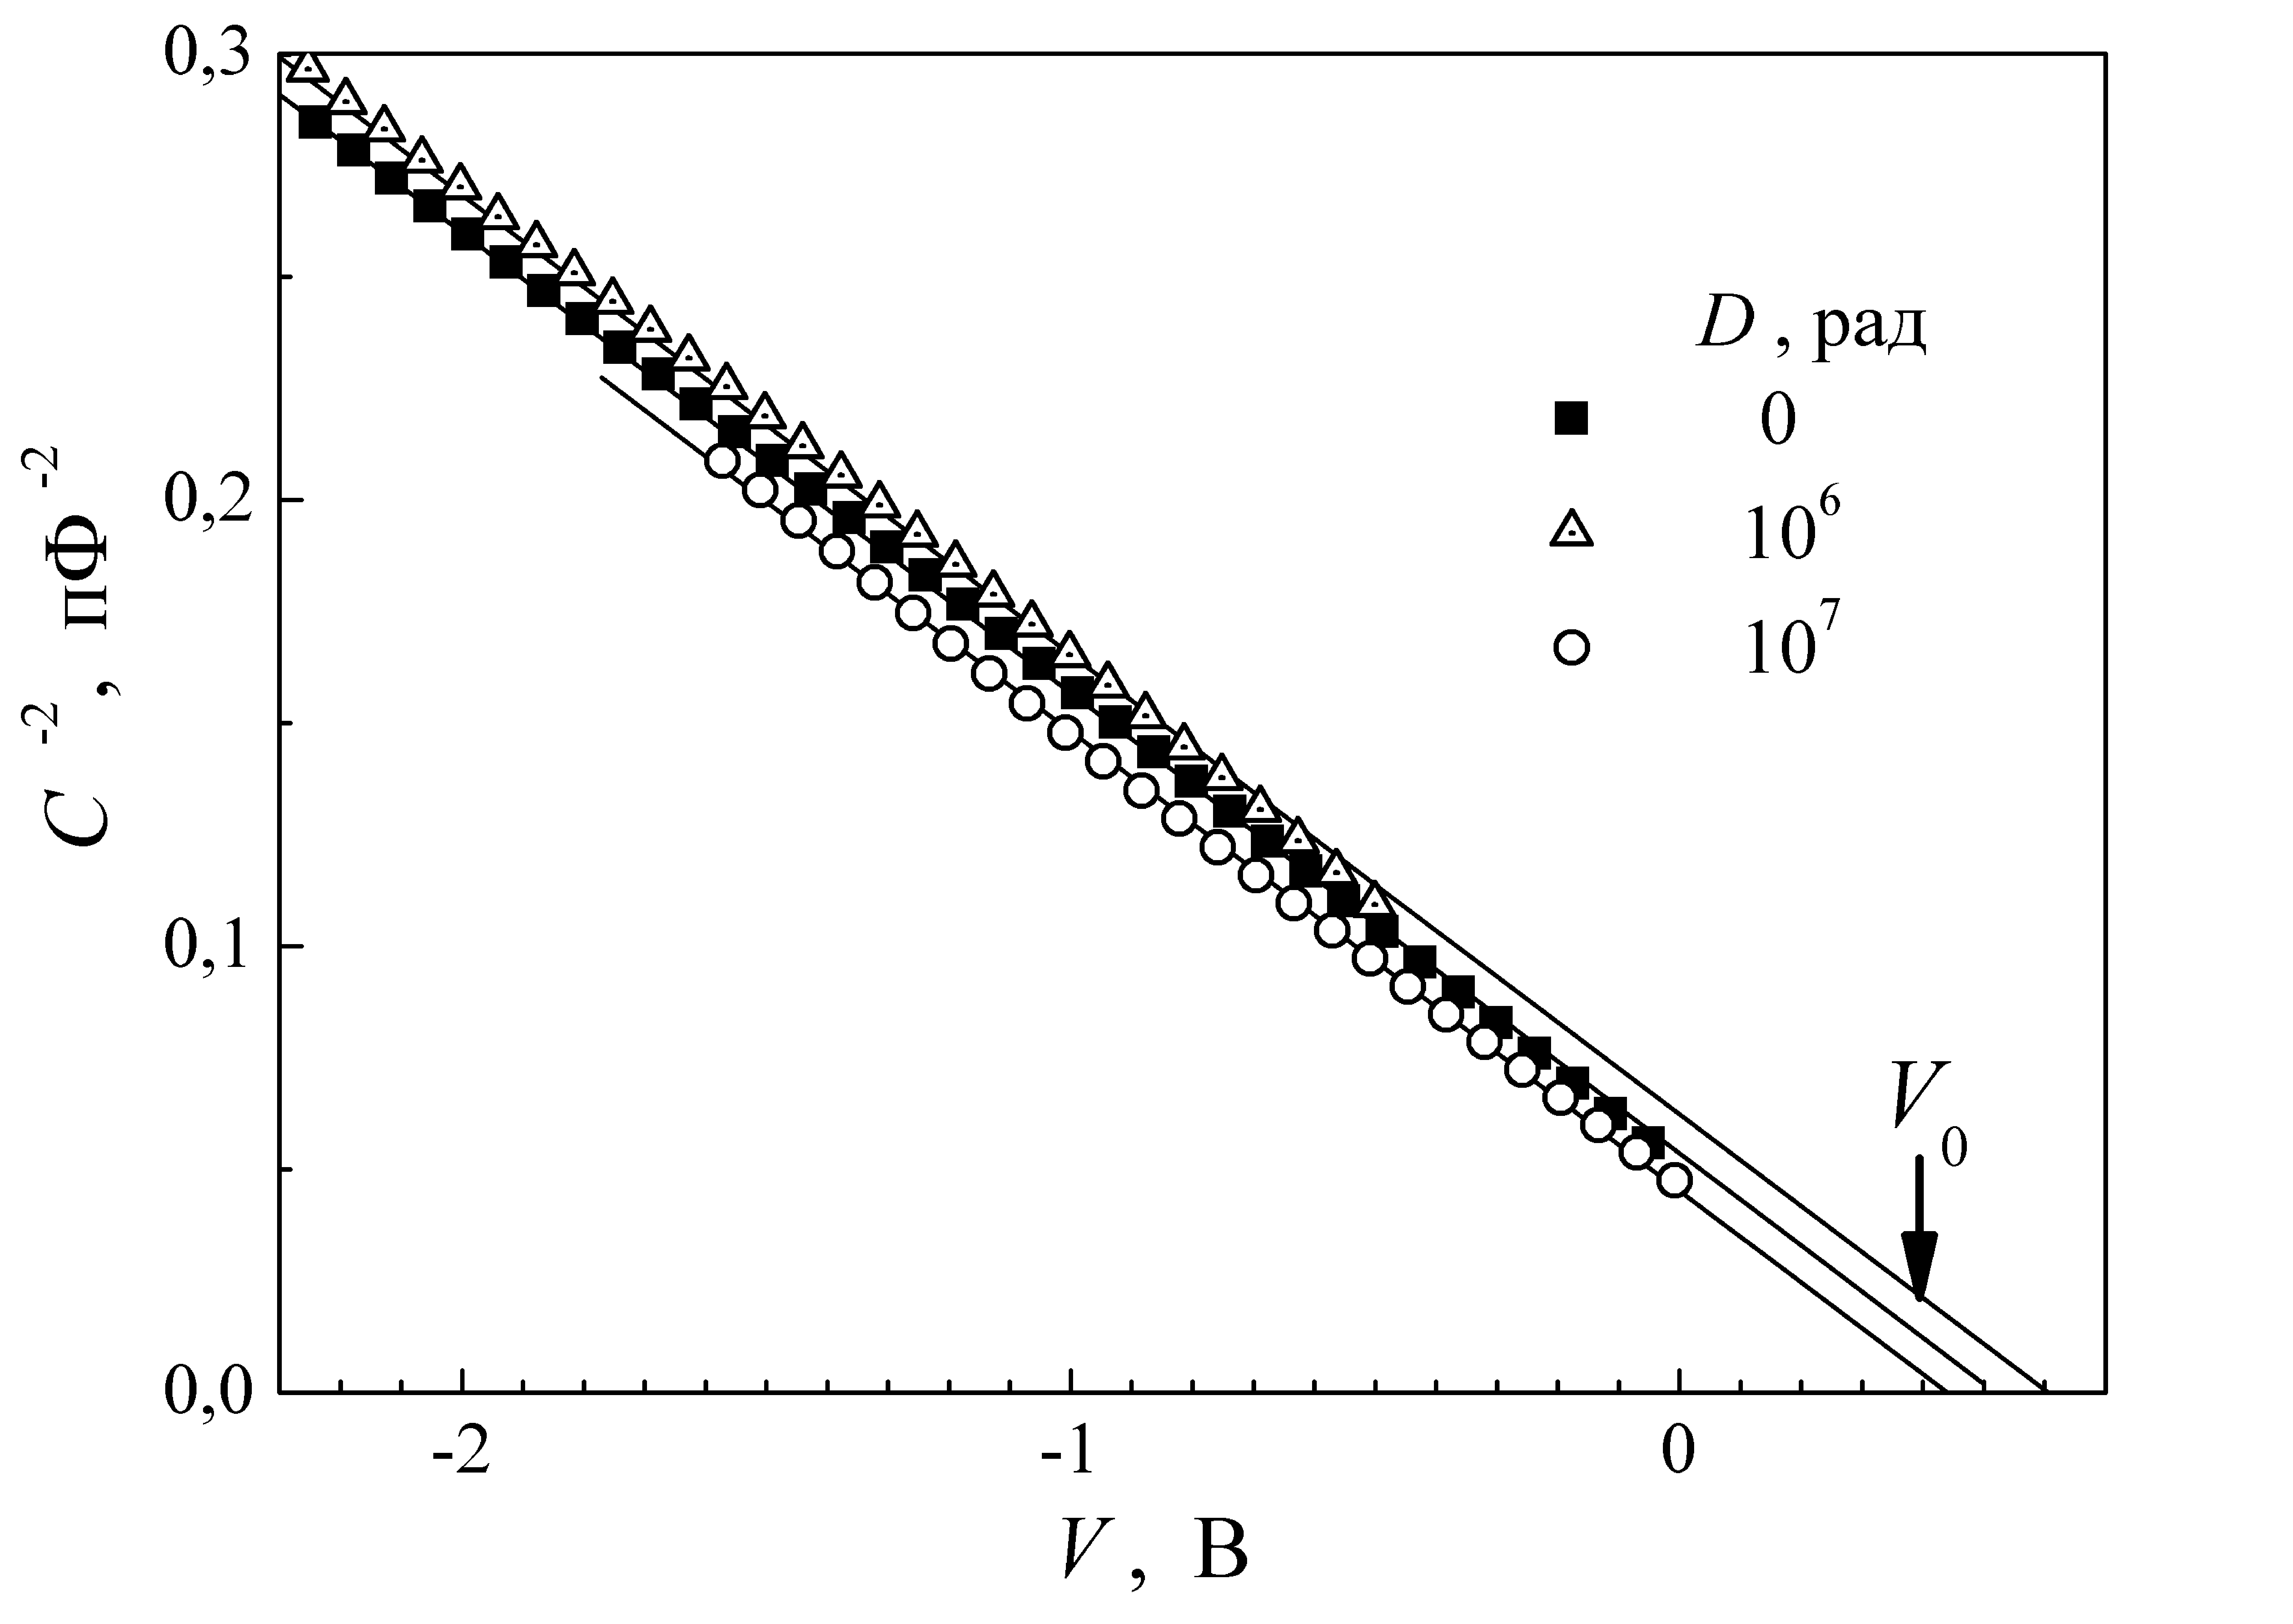
\includegraphics[width=0.6\textwidth]{figCVrad}
\caption{\label{figCVrad}
Вольт--фарадні характеристики структур Al---$n$--$n^+$--Si з різним ступенем опромінення.
Точки --- експеримент, пряма --- лінійна апроксимація
}%
\end{figure}

%виміри показали, що $N_d$ дорівнює $1.10\cdot10^{23}$ та $1.19\cdot10^{23}$ м$^{-3}$ для g6SSDA та g7SSDA, відповідно.

Нижче, поряд з отриманими результатами для опромінених зразків, нерідко наведено також дані і для вихідних,
які детально розглянуті у попередньому підрозділі.
Це зроблено з метою зручності порівнянь змін, викликаних опроміненням.


\subsection{Прямий струм у $\gamma$--опромінених кремнієвих діодах Шотткі}

На рис.~\ref{figIVrad_SDA} представлено результати вимірювань прямих гілок ВАХ структур Al---$n$--$n^+$--Si, опромінених
$\gamma$--квантами $^{60}$Co з різною величиною поглинутої дози.
Як і для неопромінених (рис.~\ref{figIV_SDA}) видно, що струм складається з двох складових,
одна з них переважає при великих зміщеннях та високих температурах; надалі для скорочення називатимемо її
<<високотемпературною компонентою струму>> (ВТКС), хоча, можливо, ця назва і не повністю віддзеркалює її поведінку.
Внесок другої стає помітним при низьких температурах ($T<250$~К) і лише при малих напругах ($V<0,2$~В);
для її позначення будемо використовувати словосполучення <<низькотемпературна компонента струму>> (НТКС).


\begin{figure}
\center
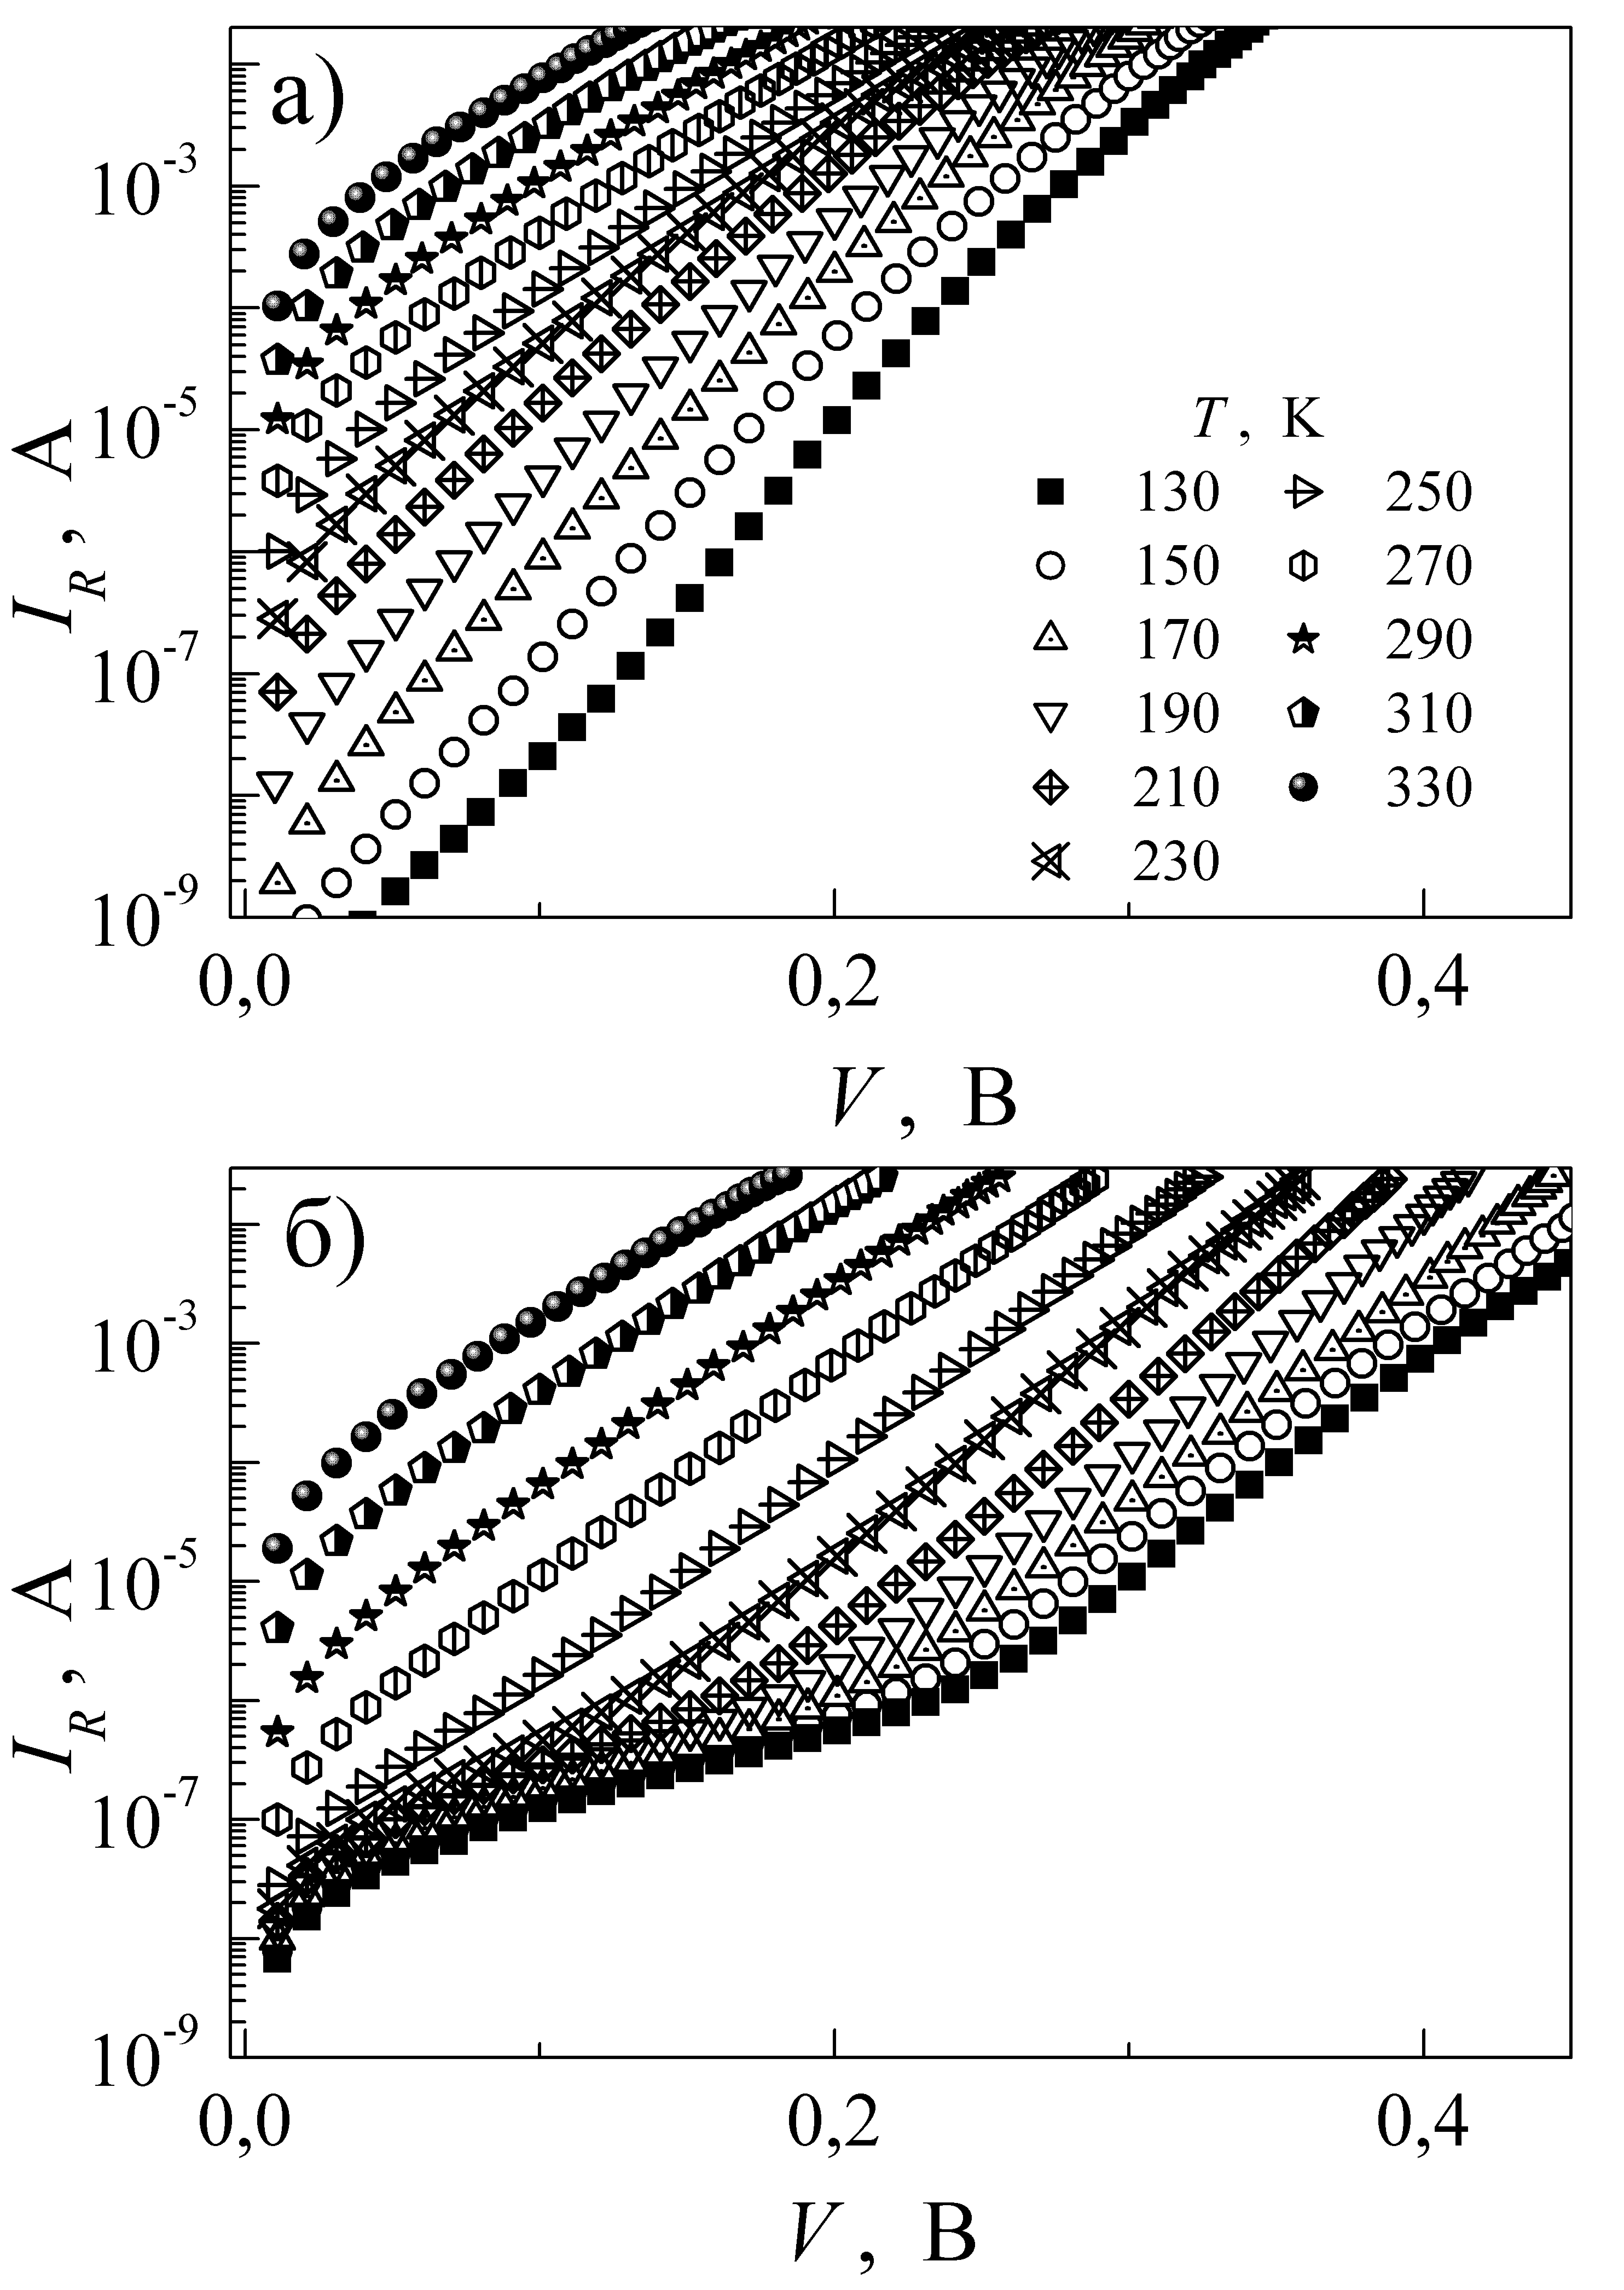
\includegraphics[width=0.55\textwidth]{figIVrad_SDA}
\caption{\label{figIVrad_SDA}
Прямі  ділянки ВАХ структур g6SSDA (a)  та g7SSDA (б) в температурному діапазоні 130$\div$330~К
}%
\end{figure}

Для ВТКС залежність $\log(I)-V$ залишається лінійною і діапазоні струмів близько трьох порядків незалежно від дози опромінення.
НТКС структур g6SSDA також є лінійною в напівлогарифмічному масштабі, тоді як при
збільшенні дози опромінення суттєво вираженим є вплив послідовного опору.

Процедура визначення параметрів збігалася з описаною в пункті~\ref{sbMSSi_NonF}.

%Для апроксимації ВАХ, як і у випадку неопромінених структур, був використаний вираз (\ref{eqSDA_IV});
%для визначення параметрів була застосована процедура, описана в пункті~\ref{sbMSSi_NonF}.

Температурні залежності ВБШ, обчисленої за формулою~(\ref{eqFb:TE}) для ВТКС, наведено на рис.~\ref{figFbTrad_SDA}.
Рисунок показує, що висота бар'єру при $\gamma$--опроміненні змінюється немонотонно:
при малих дозах $\Phi_b$ зменшується, тоді як при збільшенні $D$ спостерігається зростання цієї величини (<<спад--зростання>>) і
при $T>200$~К ВБШ при нульовому зміщенні для g7SSDA навіть перевищує відповідне значення для вихідних структур.
Дозова немонотонність може бути зумовлена зміною механізму перенесення заряду після опромінення.
А саме.
Для g7SSDA при $T>260$~К температурна залежність $\Phi_b$ майже збігається із залежністю $E_g(T)$ (рис.~\ref{figFbTrad_SDA}),
що збігається з передбаченнями теорії ТЕ через однорідний бар'єр.
Для ДШ із меншою дозою висота бар'єру зростає з підвищенням температури, що не може бути поясненим у наближенні цієї теорії.


\begin{figure}
\center
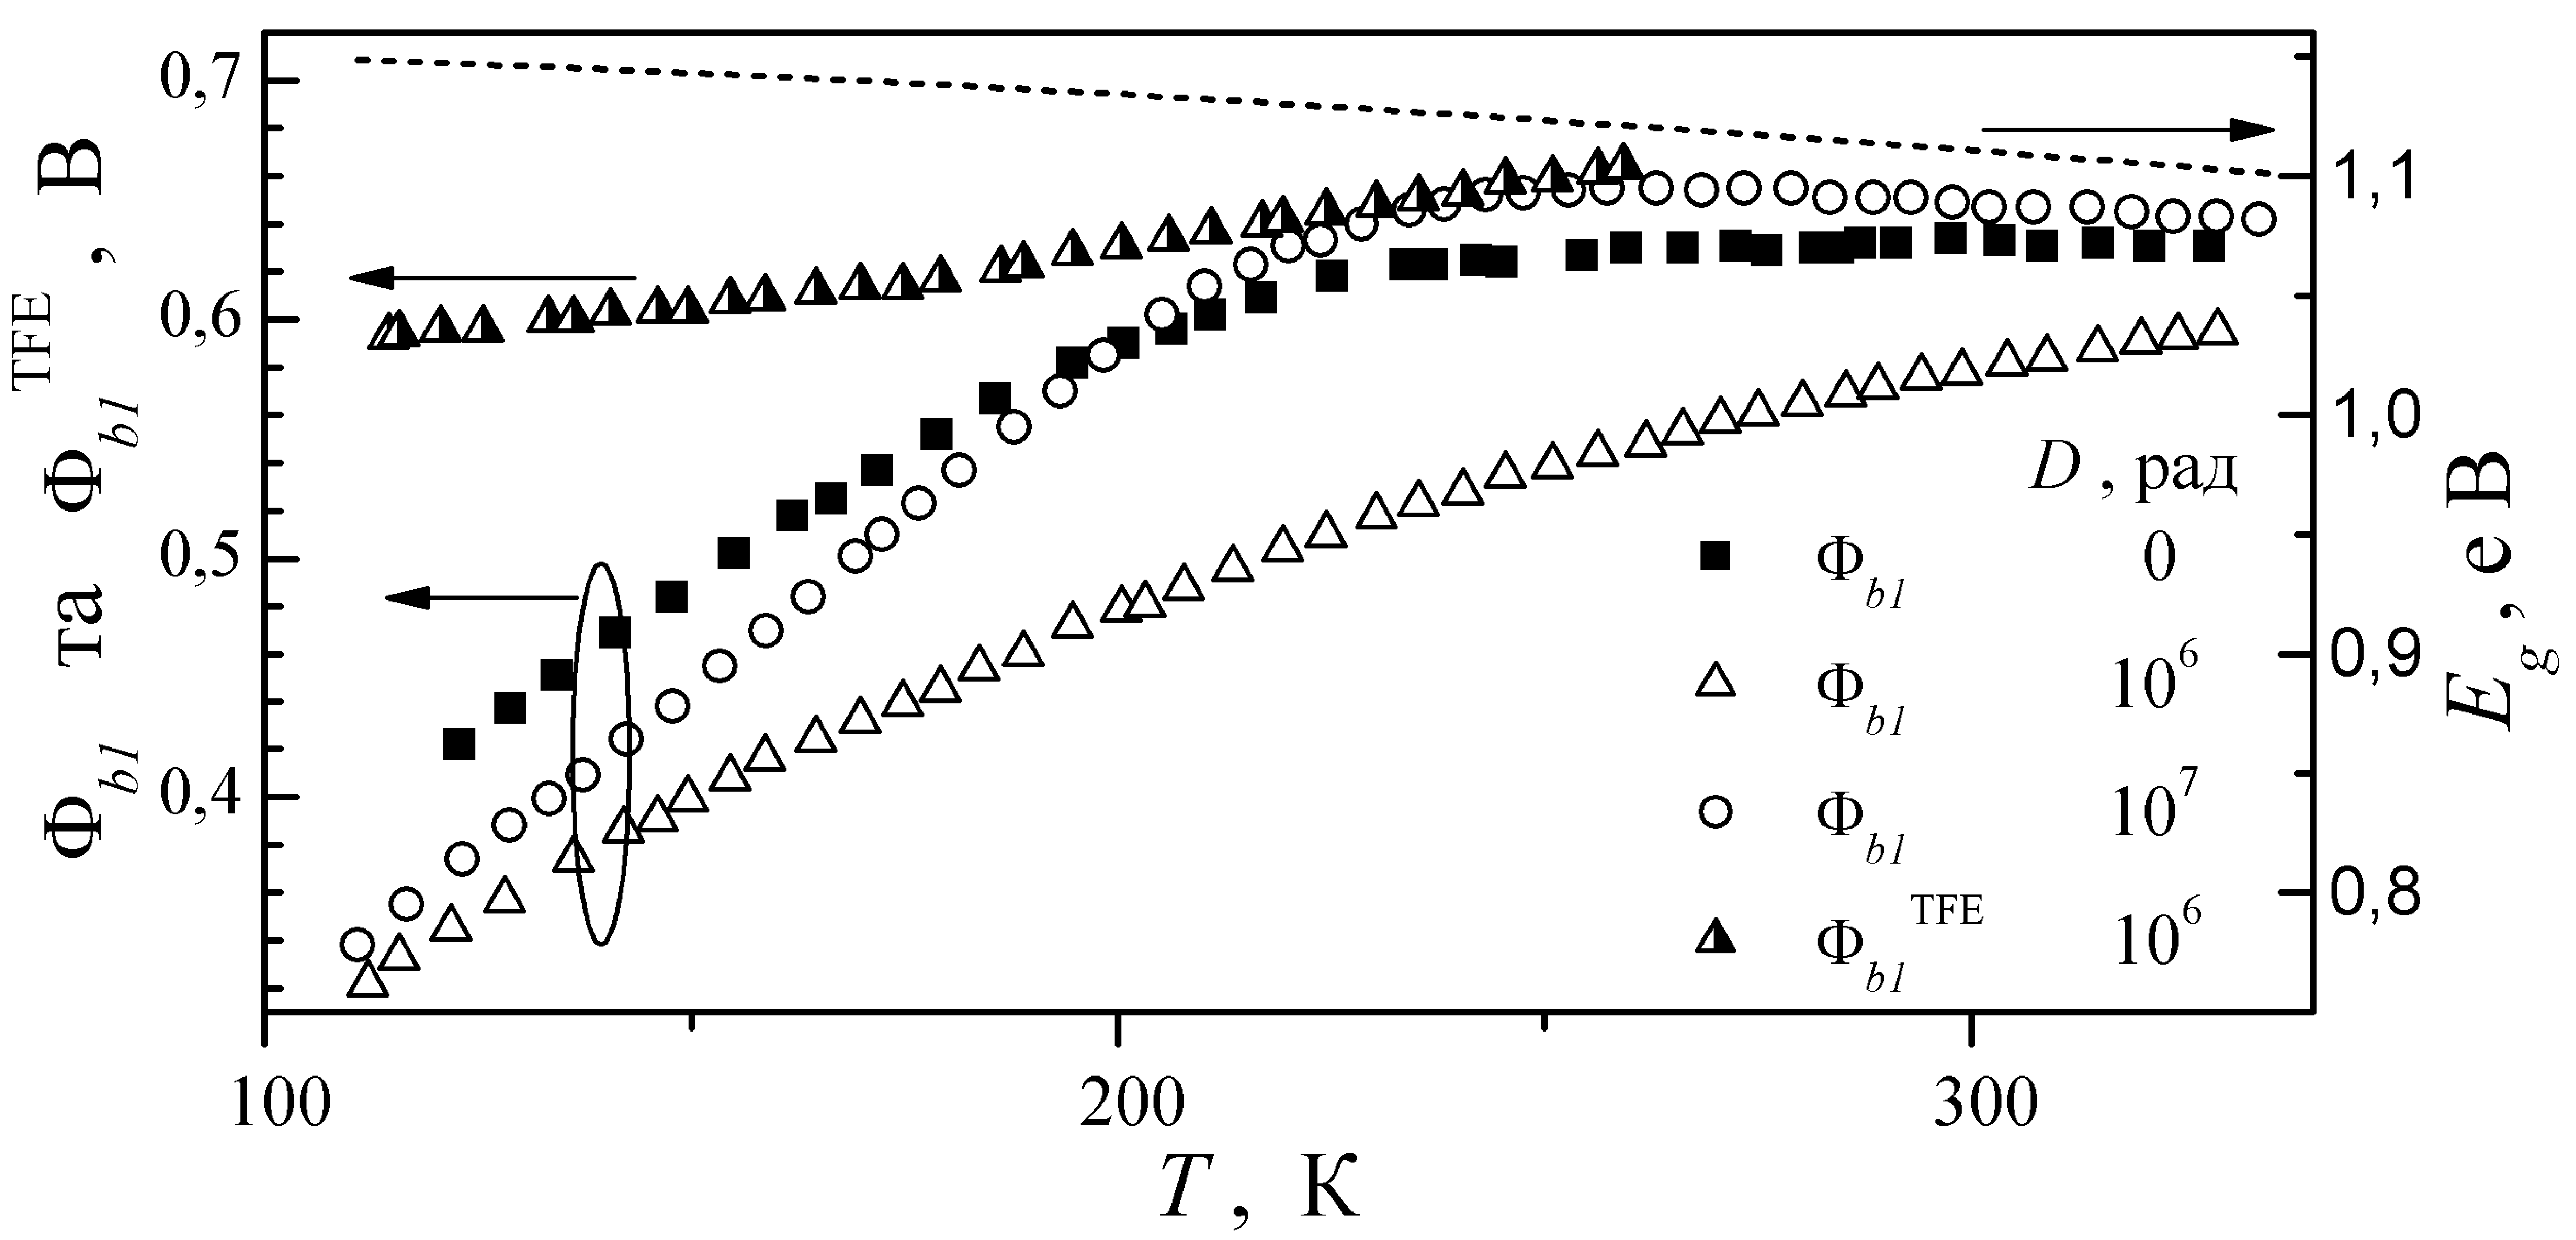
\includegraphics[width=0.9\textwidth]{figFbTrad_SDA}
\caption{\label{figFbTrad_SDA}
Температурні залежності висоти бар'єру, розрахованої в рамках моделі ТЕ та ТПЕ
для ВТКС зразків SSDA (квадрати),
g6SSDA (трикутники) та g7SSDA (кола).
Пунктирна лінія (права вісь)--- залежність ширини забороненої зони кремнію
}%
\end{figure}


Для оцінки можливого впливу неоднорідності контакту на рис.~\ref{figFbfbrad_SDA} наведено температурні
залежності  $\Phi_{b}^\mathrm{FB}$, побудовані відповідно до формули~(\ref{eqFbfb}).
На відміну від неопромінених структур, для яких залежність ВБШ в наближенні плоских зон майже збігалася
з поведінкою $E_g$ у всьому температурному діапазоні (рис.~\ref{figFbfb_SDA}),
для g6SSDA  та g7SSDA поведінки $\Phi_{b}^\mathrm{FB}$ та ширини забороненої зони схожі лише при $T>260$~К та $T>240$~К, відповідно.
Відтак, лише в цих діапазонах можливе домінування процесів ТЕ і саме для цих інтервалів температур побудовані
залежності $\Phi_b$ від $q/2kT$, $(n_\mathrm{id}^{-1}-1)$ від $q/2kT$ та $\Phi_b$ від $n_\mathrm{id}$,
представлені на
рис.~\ref{figFbNrad_SDA}.

\begin{figure}
\center
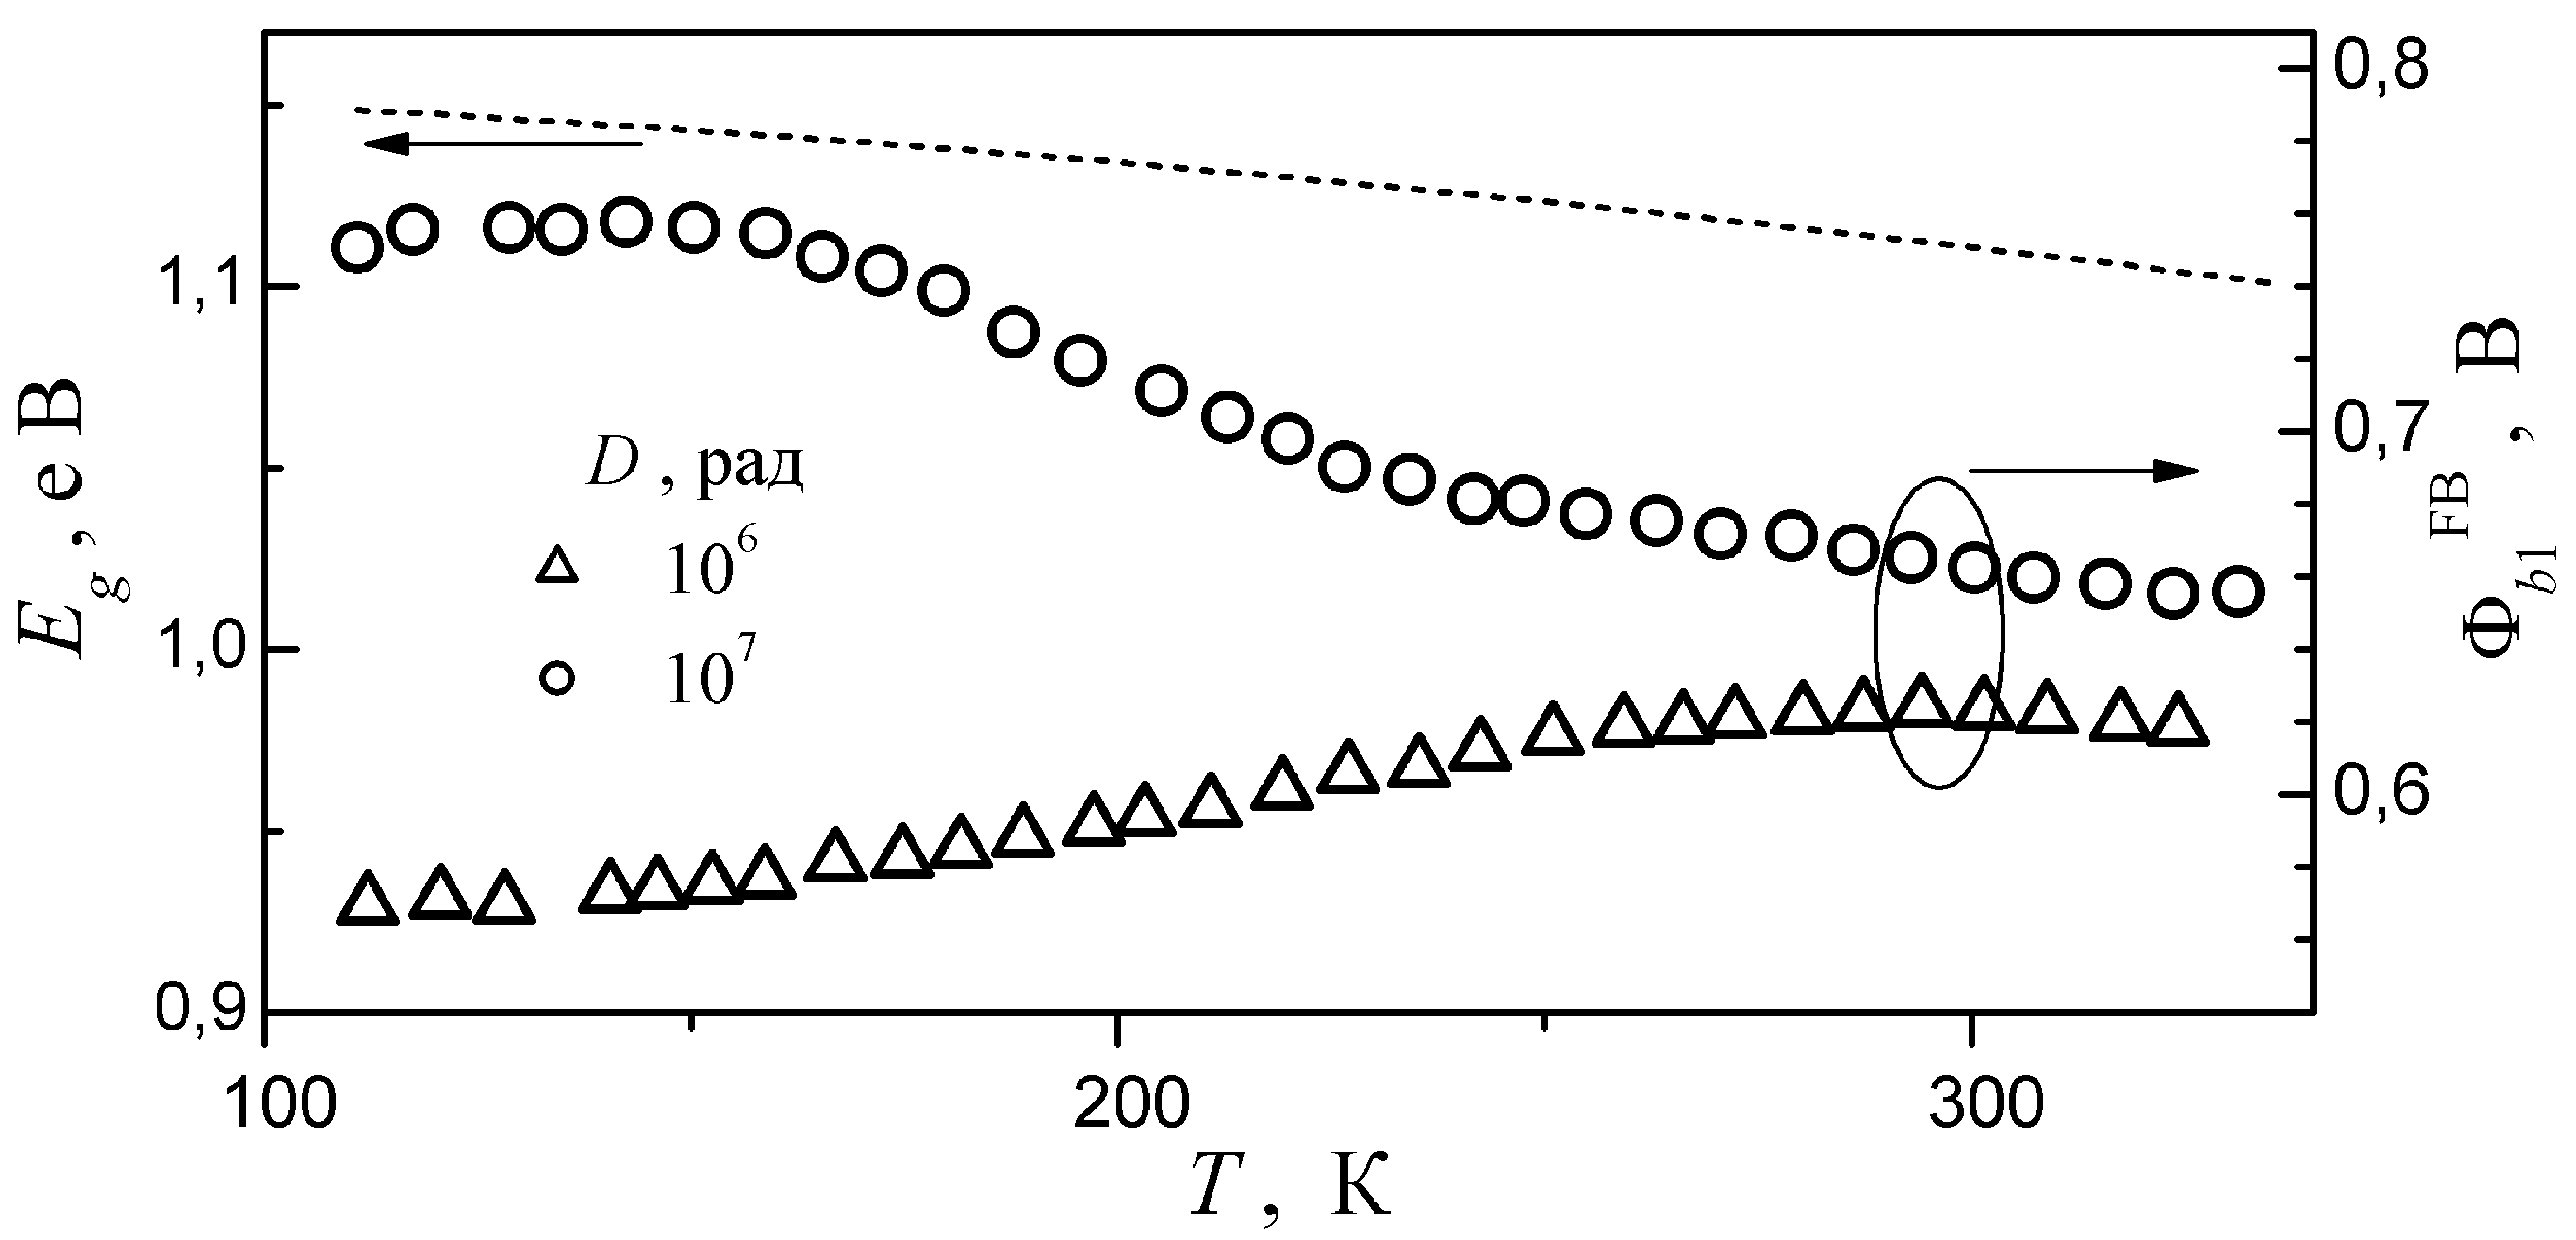
\includegraphics[width=0.8\textwidth]{figFbfbrad_SDA}
\caption{\label{figFbfbrad_SDA}
Температурні залежності ВБШ в наближені плоских зон (точки, права вісь), розрахованої
для ВТКС структур
g6SSDA (трикутники) та g7SSDA (кола),
та ширини забороненої зони (пунктир, ліва вісь)
}%
\end{figure}



\begin{figure}
\center
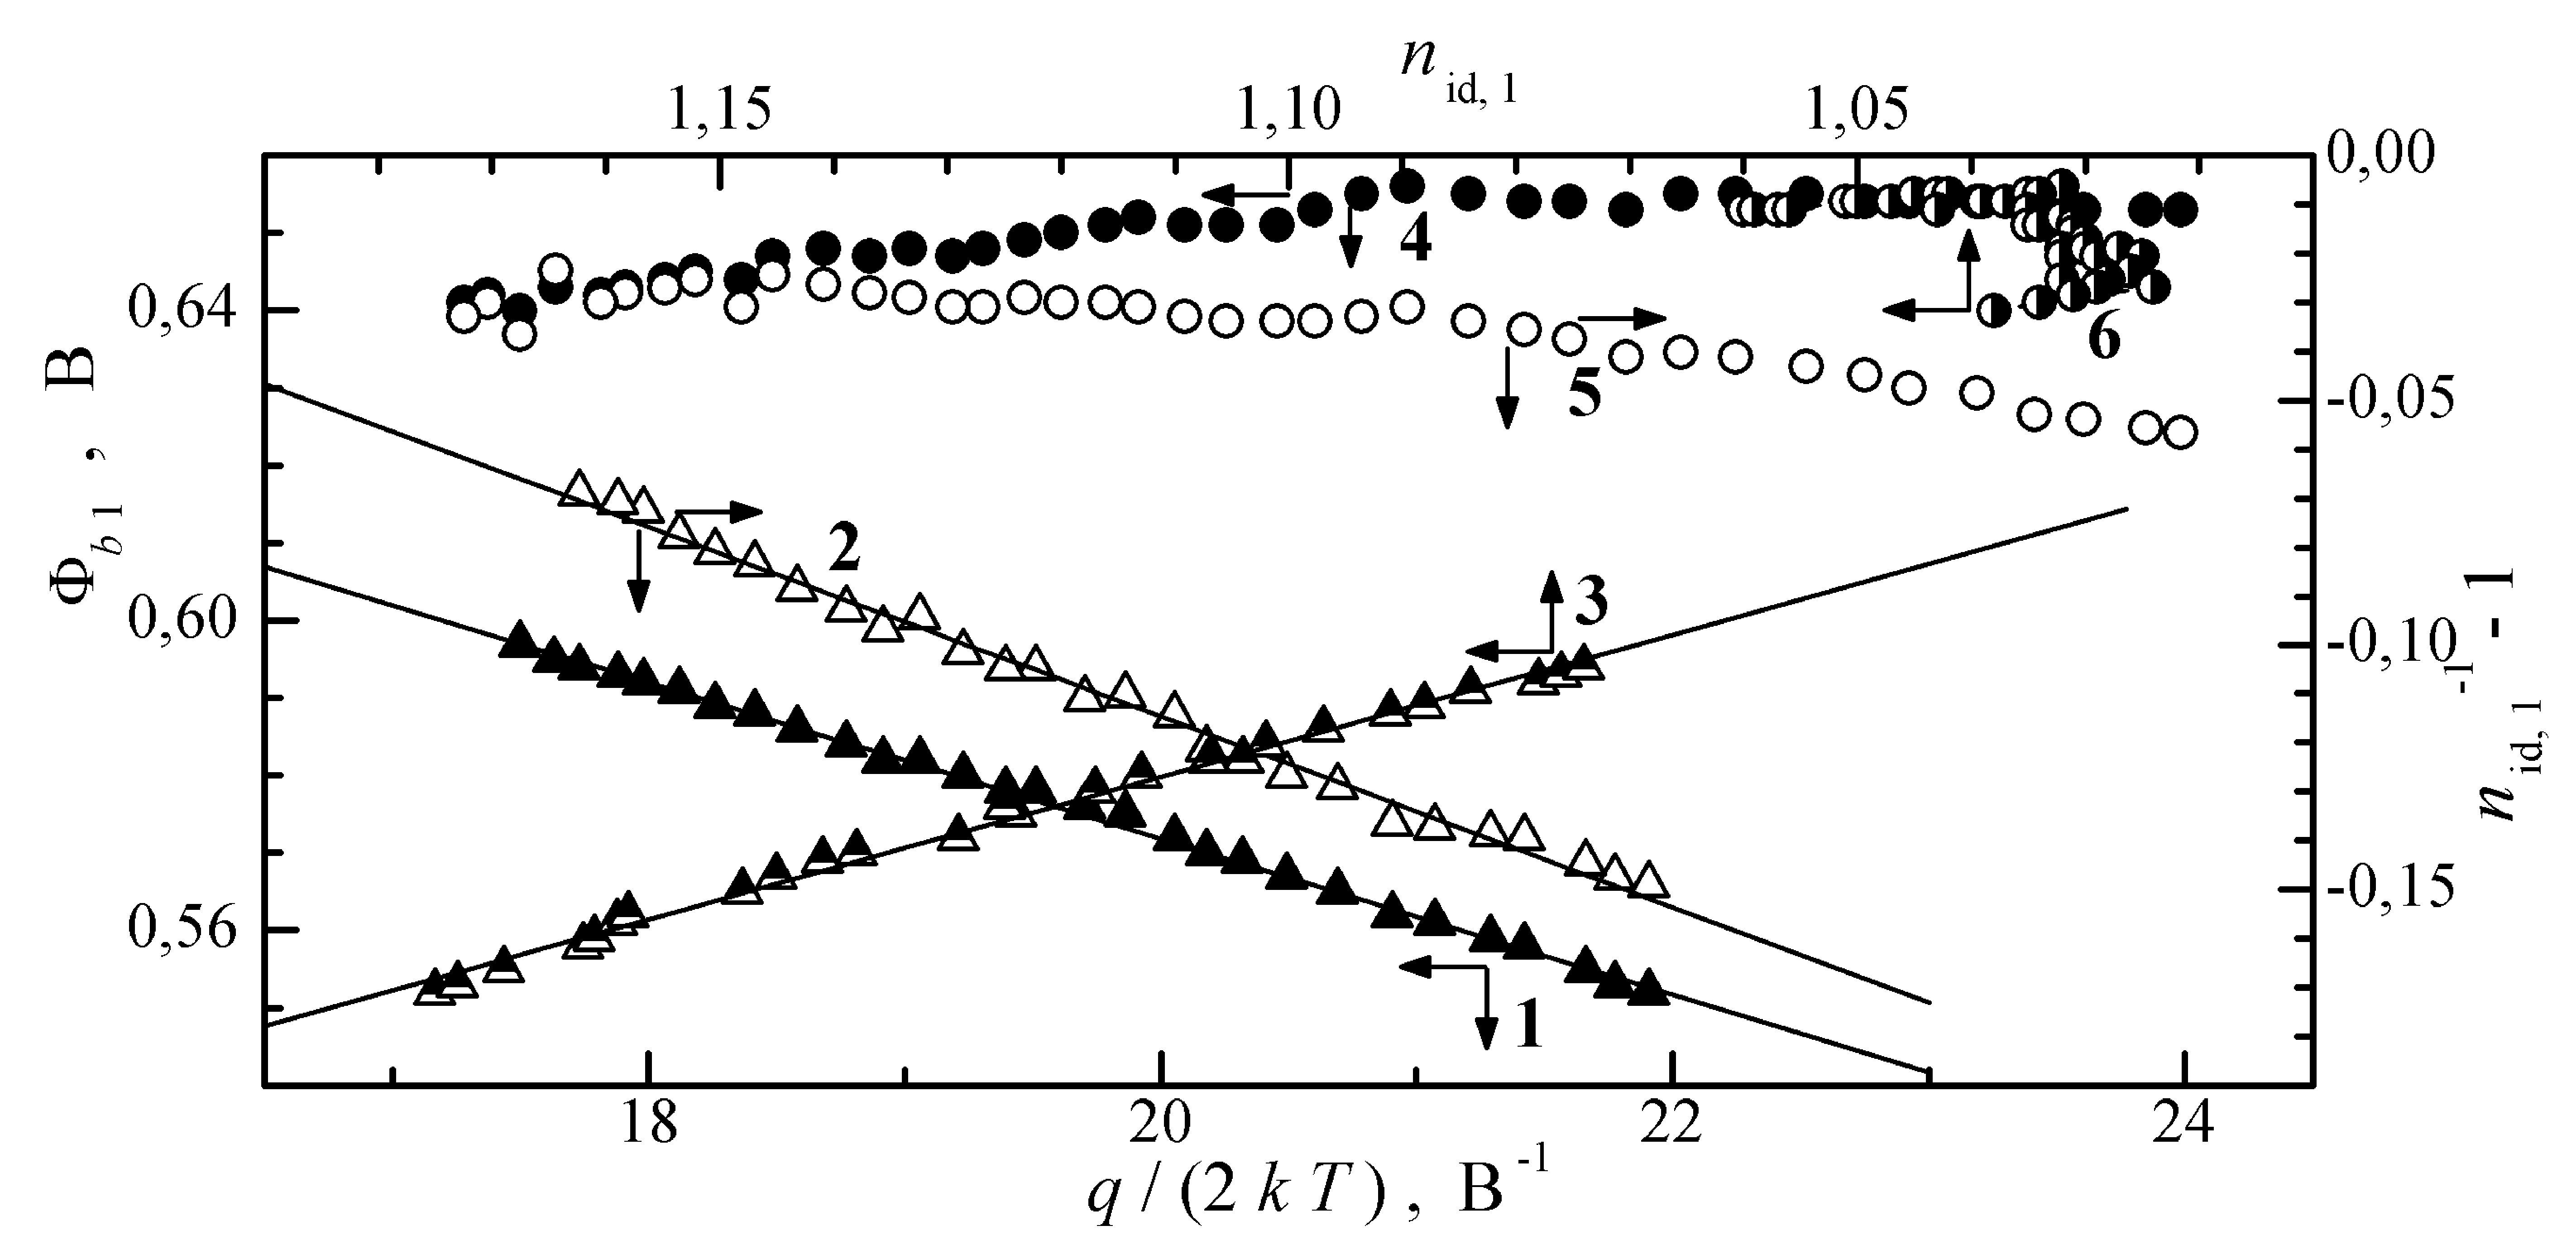
\includegraphics[width=0.9\textwidth]{figFbNrad_SDA}
\caption{\label{figFbNrad_SDA}
Залежності величин $\Phi_{b1}$ (криві 1 та 4, заповнені точки) та
$n_{\mathrm{id},1}^{-1}-1$ (криві 2 та 5, незаповнені точки) від оберненої температури
та залежність ВБШ від фактора неідеальності (криві 3 та 6, напівзаповнені точки)
$D$, рад: 10$^6$ (1--3), 10$^7$ (4--6).
Точки --- експеримент,
прямі --- лінійна апроксимація %за методом найменших квадратів
}%
\end{figure}

Якщо має місце ТЕ через неоднорідний бар'єр, то залежності на рис.~\ref{figFbNrad_SDA} повинні бути лінійними \cite{Werner,Tung:PhysRev,Schmitsdorf}.
З рисунка видно, що очікуваний вигляд спостерігається лише для g6SSDA,
а відтак згаданий механізм домінує в Al---$n$--$n^+$--Si лише при поглинутій дозі $\gamma$--квантів близько $10^6$~рад при $T>260$~К.
Обчислені в наближені моделі струму через неоднорідний контакт висота бар'єру за межами патчів,
її стандартне відхилення та коефіцієнти польової залежності розподілу ВБШ наведено в табл.~\ref{tabSDAParRad}.
Зауважимо, що отримані дані свідчать про збільшення середнього значення висоти бар'єру та
стандартного відхилення параметрів патчів при опроміненні ДШ $\gamma$--квантами з дозою $10^6$~рад.

\begin{table}
%\renewcommand{\arraystretch}{1.3}
\caption{Параметри, визначені з ВАХ структур Al---$n$--$n^+$--Si в наближенні теорії TE}
\label{tabSDAParRad}
\centering
\begin{tabular}{|l|c|c|c|}
\hline
$D$, рад & 0&10$^6$&10$^7$\\ \hline
Діапазон температур, K&230$\div$330&260$\div$330&260$\div$330\\ \hline
$\sigma_{\Phi0}$, мВ&$40\pm5$&$100\pm1$&--\\ \hline
$\rho_2$, $10^{-2}$&$12\pm1$&$27\pm1$&--\\ \hline
$\rho_3$, мВ&$8,0\pm0,3$&$19,0\pm0,4$&--\\ \hline
$\Phi_b^0$, мВ \textsuperscript{ a)}&$663\pm3$&$772\pm2$&--\\ \hline
$\Phi_b^0$, мВ &$662\pm3$ \textsuperscript{ б)}&$772\pm2$ \textsuperscript{ б)}&$710\pm3$ \textsuperscript{ в)}\\ \hline
$\Phi_{b,CV}$, мВ &$683\pm2$&$770\pm5$&$604\pm4$\\ \hline
$A^*$, A$\cdot$см$^{-2}\cdot$K$^{-2}$&$112\pm20$&$115\pm20$&$1200\pm300$\\
\hline
$\Phi_{b,p}$, мВ&$54\pm4$&$74\pm6$&--\\ \hline
$f_p$, $10^{-13}$&$8\pm1$&$8\pm1$&--\\ \hline
\multicolumn{4}{l}{\textsuperscript{ a)} \emph{за залежністю $\Phi_b=f(\frac{1}{2kT})$}} \\
\multicolumn{4}{l}{\textsuperscript{ б)} \emph{за модифікованою залежністю Річардсона (\ref{eqRich:Mod}) }} \\
\multicolumn{4}{l}{\textsuperscript{ в)} \emph{за звичайною залежністю Річардсона (\ref{figRich_SDA})}} \\
\end{tabular}
\end{table}


Для g7SSDA всі залежності на рис.~\ref{figFbNrad_SDA} не є лінійними, а отже модель ТЕ через неоднорідний бар'єр для цього випадку незастосовна.
Про це свідчать і температурні залежності ВБШ, розраховані для НТКС --- рис.~\ref{figFb2Trad_SDA}.
Дійсно, у пункті~\ref{sbMSSi_NonF} вже згадувалося, що поява додаткового струму при низьких температурах у випадку неоднорідного контакту
зумовлена ефективним проходженням носіїв заряду через патчі, причому висота бар'єру, яка визначається з ВАХ традиційним способом має лінійно зростати з температурою
--- див. вираз (\ref{eqFbFbp}).
Як видно з рисунку, для досліджених структур лінійна залежність спостерігається незалежно від дози.
Проте якщо для g6SSDA обчислені дані свідчать про зростання висоти бар'єру в області патчу та про незмінність загальної площі, яку вони займають (див. дані табл.~\ref{tabSDAParRad}),
то для g7SSDA отримане в рамках моделі від'ємне значення висоти бар'єру $\Phi_{b,p}\approx-9$~мВ не має фізичного змісту.
%Тобто в структурах, де поглинута доза складає $10^7$~рад перенесення заряду відбувається в рамках класичного механізму ТЕ.



\begin{figure}
\center
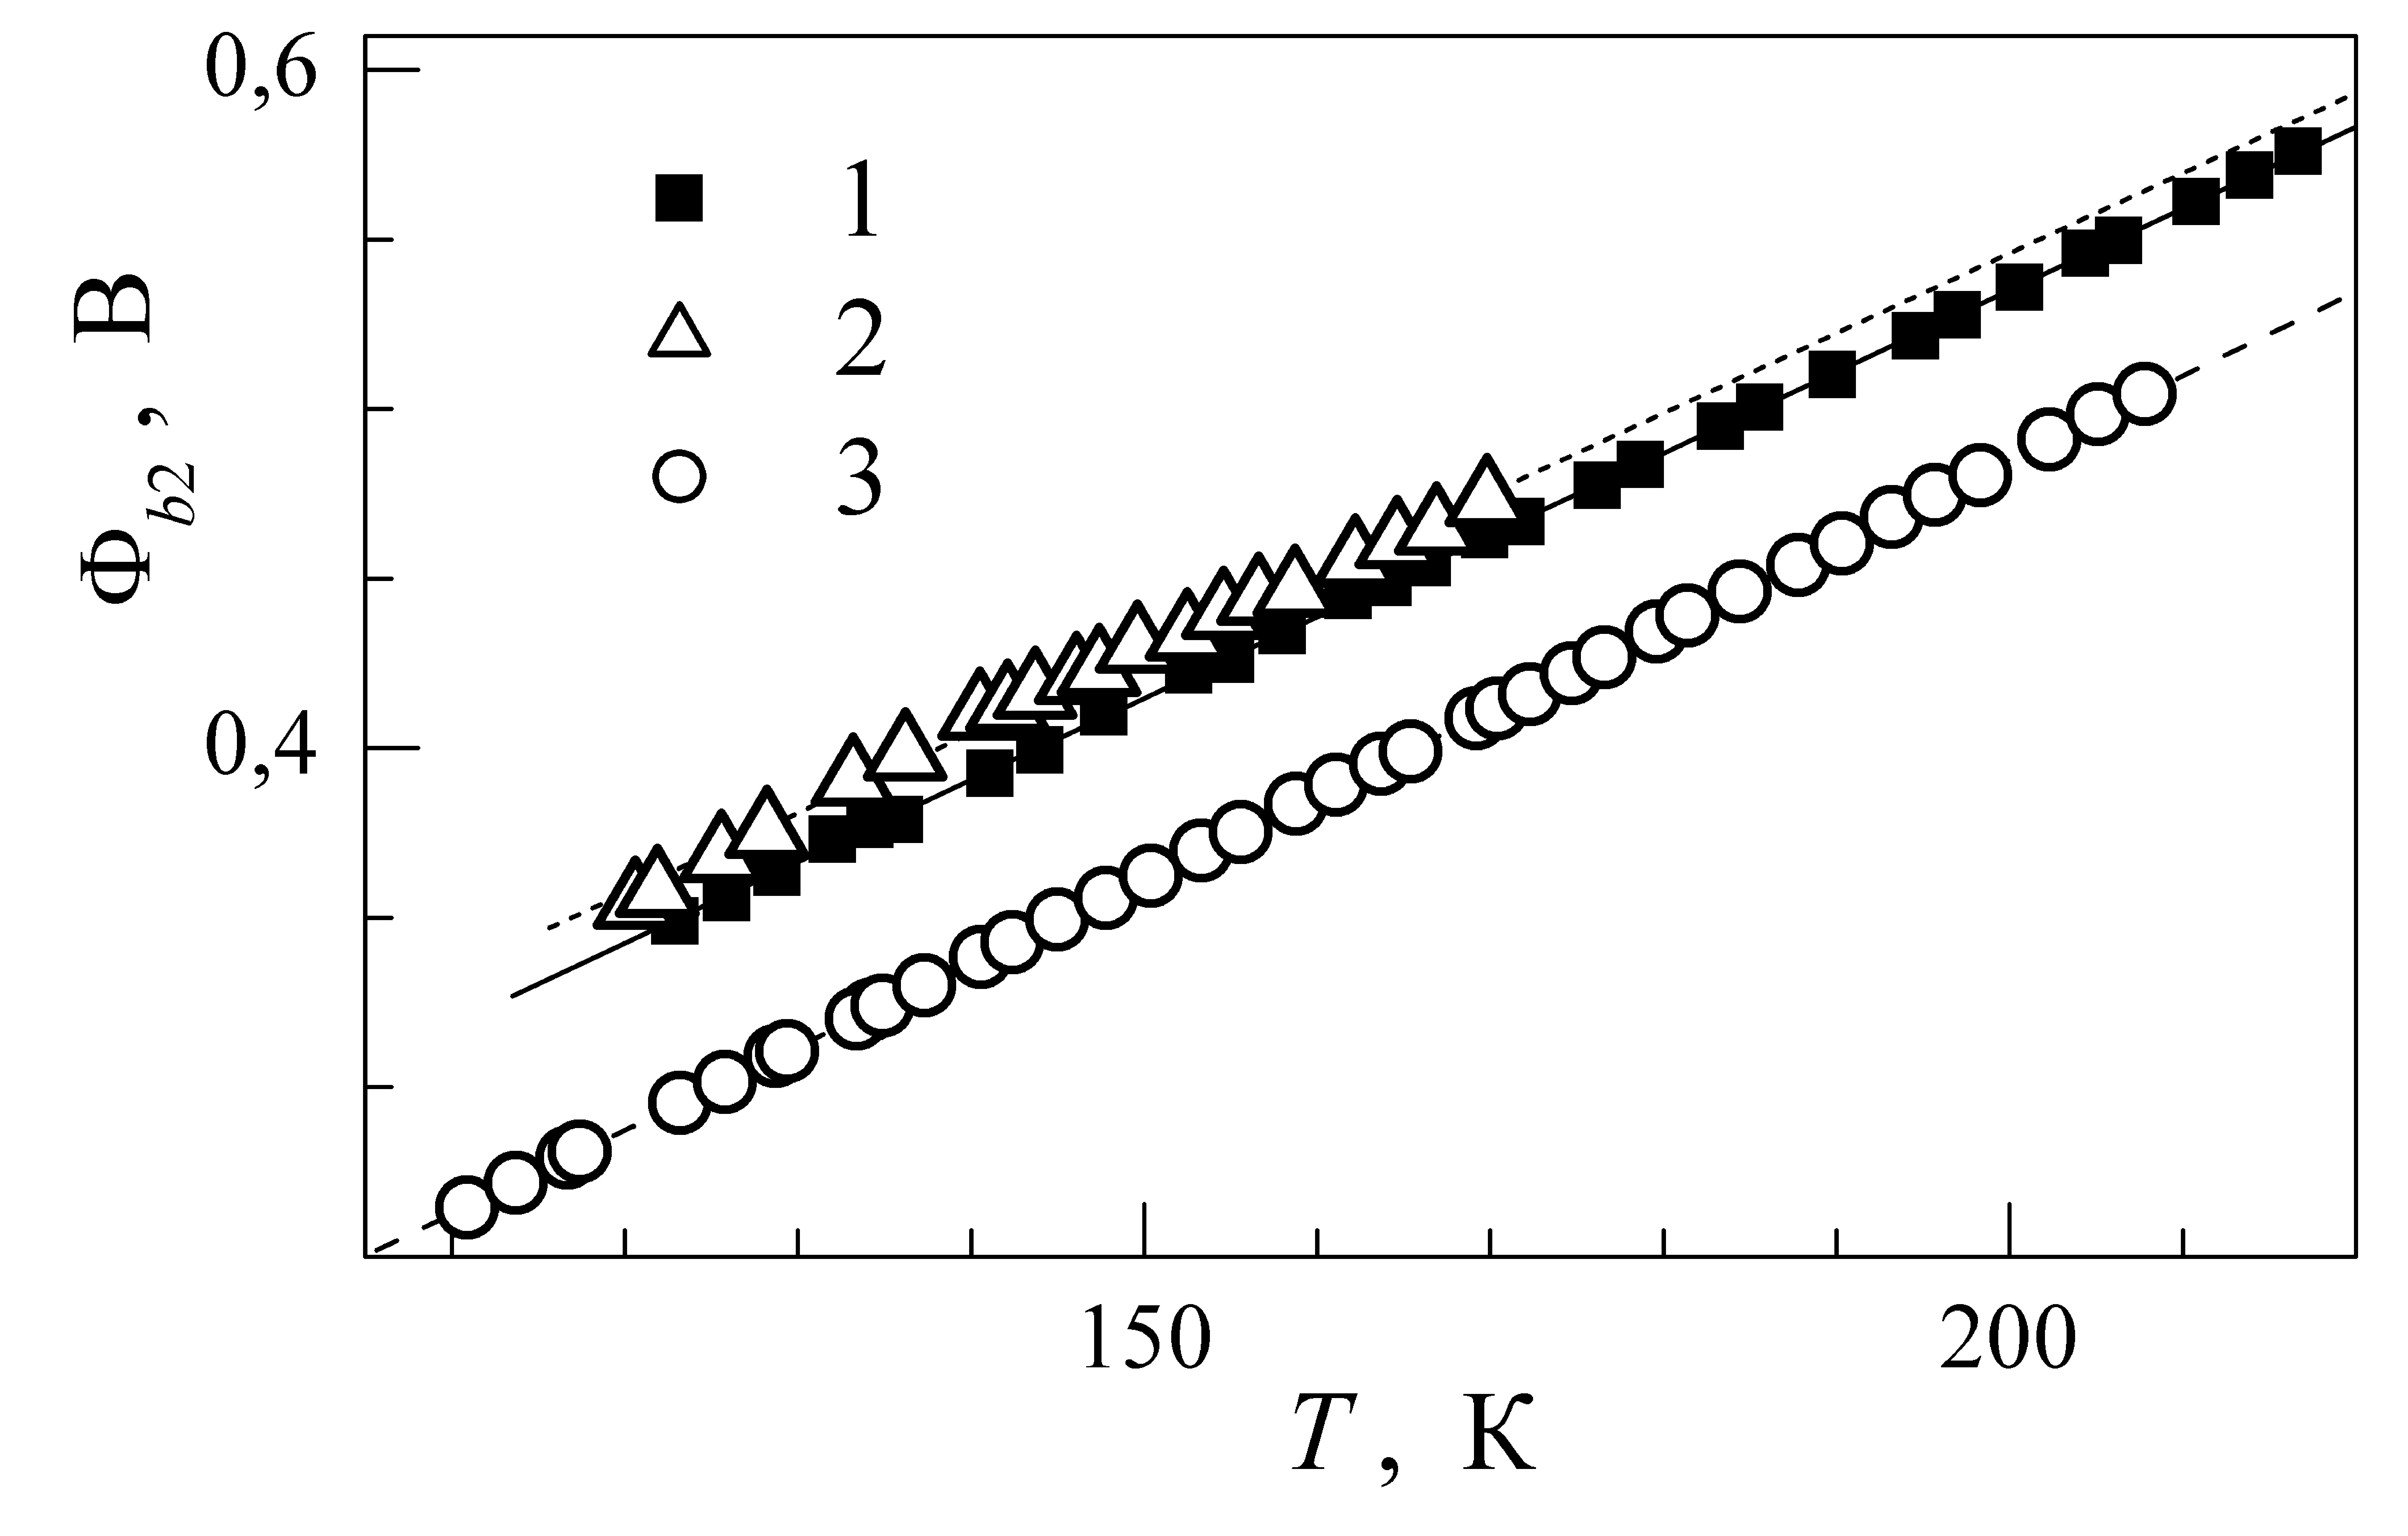
\includegraphics[width=0.65\textwidth]{figFb2Trad_SDA}
\caption{\label{figFb2Trad_SDA}
Температурні залежності висоти бар'єру, розрахованої в рамках моделі ТЕ
для низькотемпературної компоненти струму зразків SSDA (квадрати),
g6SSDA (трикутники) та g7SSDA (кола).
Прямі  --- лінійна апроксимація %(суцільна для SSDA, пунктирна для g6SSDA та
%штрихована для g7SSDA)
}%
\end{figure}

Отже, для оцінки величини $A^*$ для структур із низьким рівнем $\gamma$--опромінення доцільно використовувати
модифіковану залежність Річардсона (рис.~\ref{figRichMrad_SDA}), тоді як для g7SSDA такий підхід не є виправданим.
На рисунку також наведено звичайну залежність Річардсона для g7SSDA, яка хоч і є лінійною,
проте розраховане за її допомогою значення $A^*$ (табл.~\ref{tabSDAParRad}) суттєво відрізняється від очікуваного.
Крім того, оцінена таким чином висота бар'єру перевищує значення, отримане з ВФХ, що також суперечить очікуванням --- див. пункт~\ref{sbMSSi_NonF}.
Це може свідчити про наявність додаткового, крім ТЕ через однорідний контакт,
механізму перенесення заряду в g7SSDA.
Зауважимо, що отримане значення сталої Річардсона для g6SSDA збігається з відомою  величиною.

\begin{figure}
\center
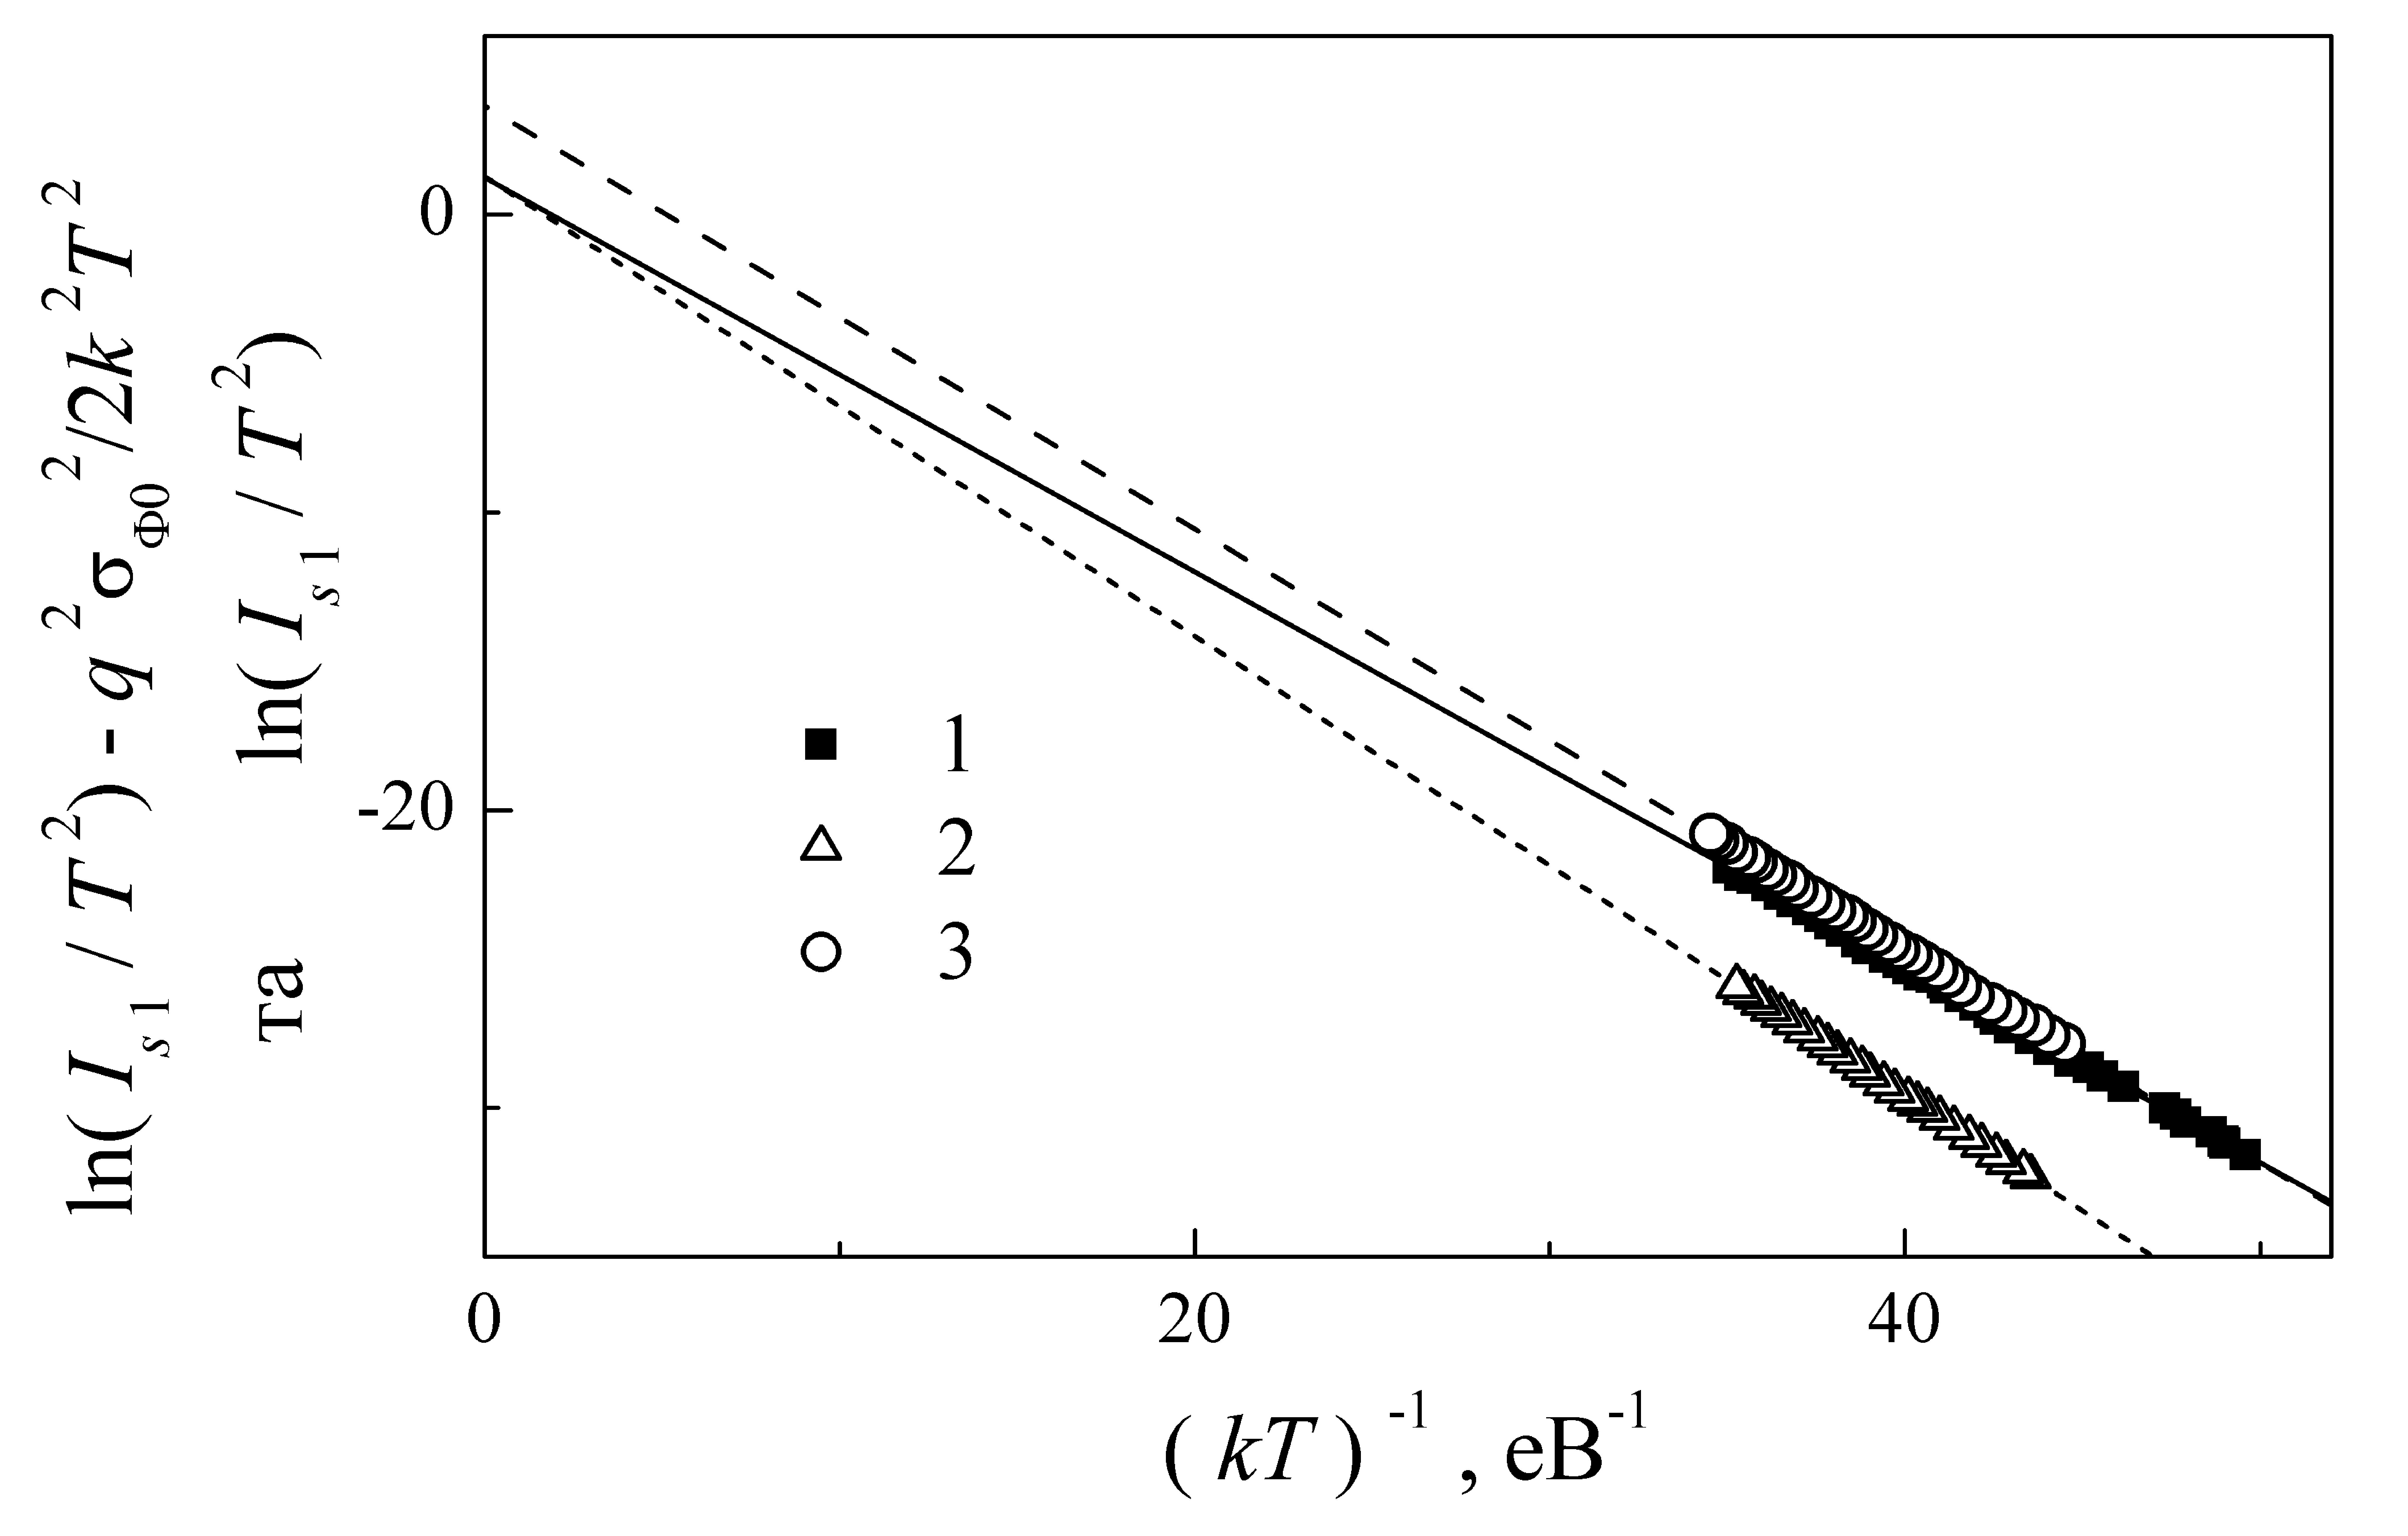
\includegraphics[width=0.7\textwidth]{figRichMrad_SDA}
\caption{\label{figRichMrad_SDA}
Модифіковані (криві 1 та 2, структури SSDA та g6SSDA, відповідно) та звичайні (3, g7SSDA) залежності Річардсона, розраховані для ВТКС при 230$\div$330~K~(1) та 260$\div$330~K~(2, 3).
$\sigma_{\Phi,0}$, мВ: 99 (1) та 100 (2).
Прямі  --- лінійна апроксимація (суцільна для SSDA, пунктирна для g6SSDA та
штрихована для g7SSDA)
}%
\end{figure}

\begin{figure}[b]
\center
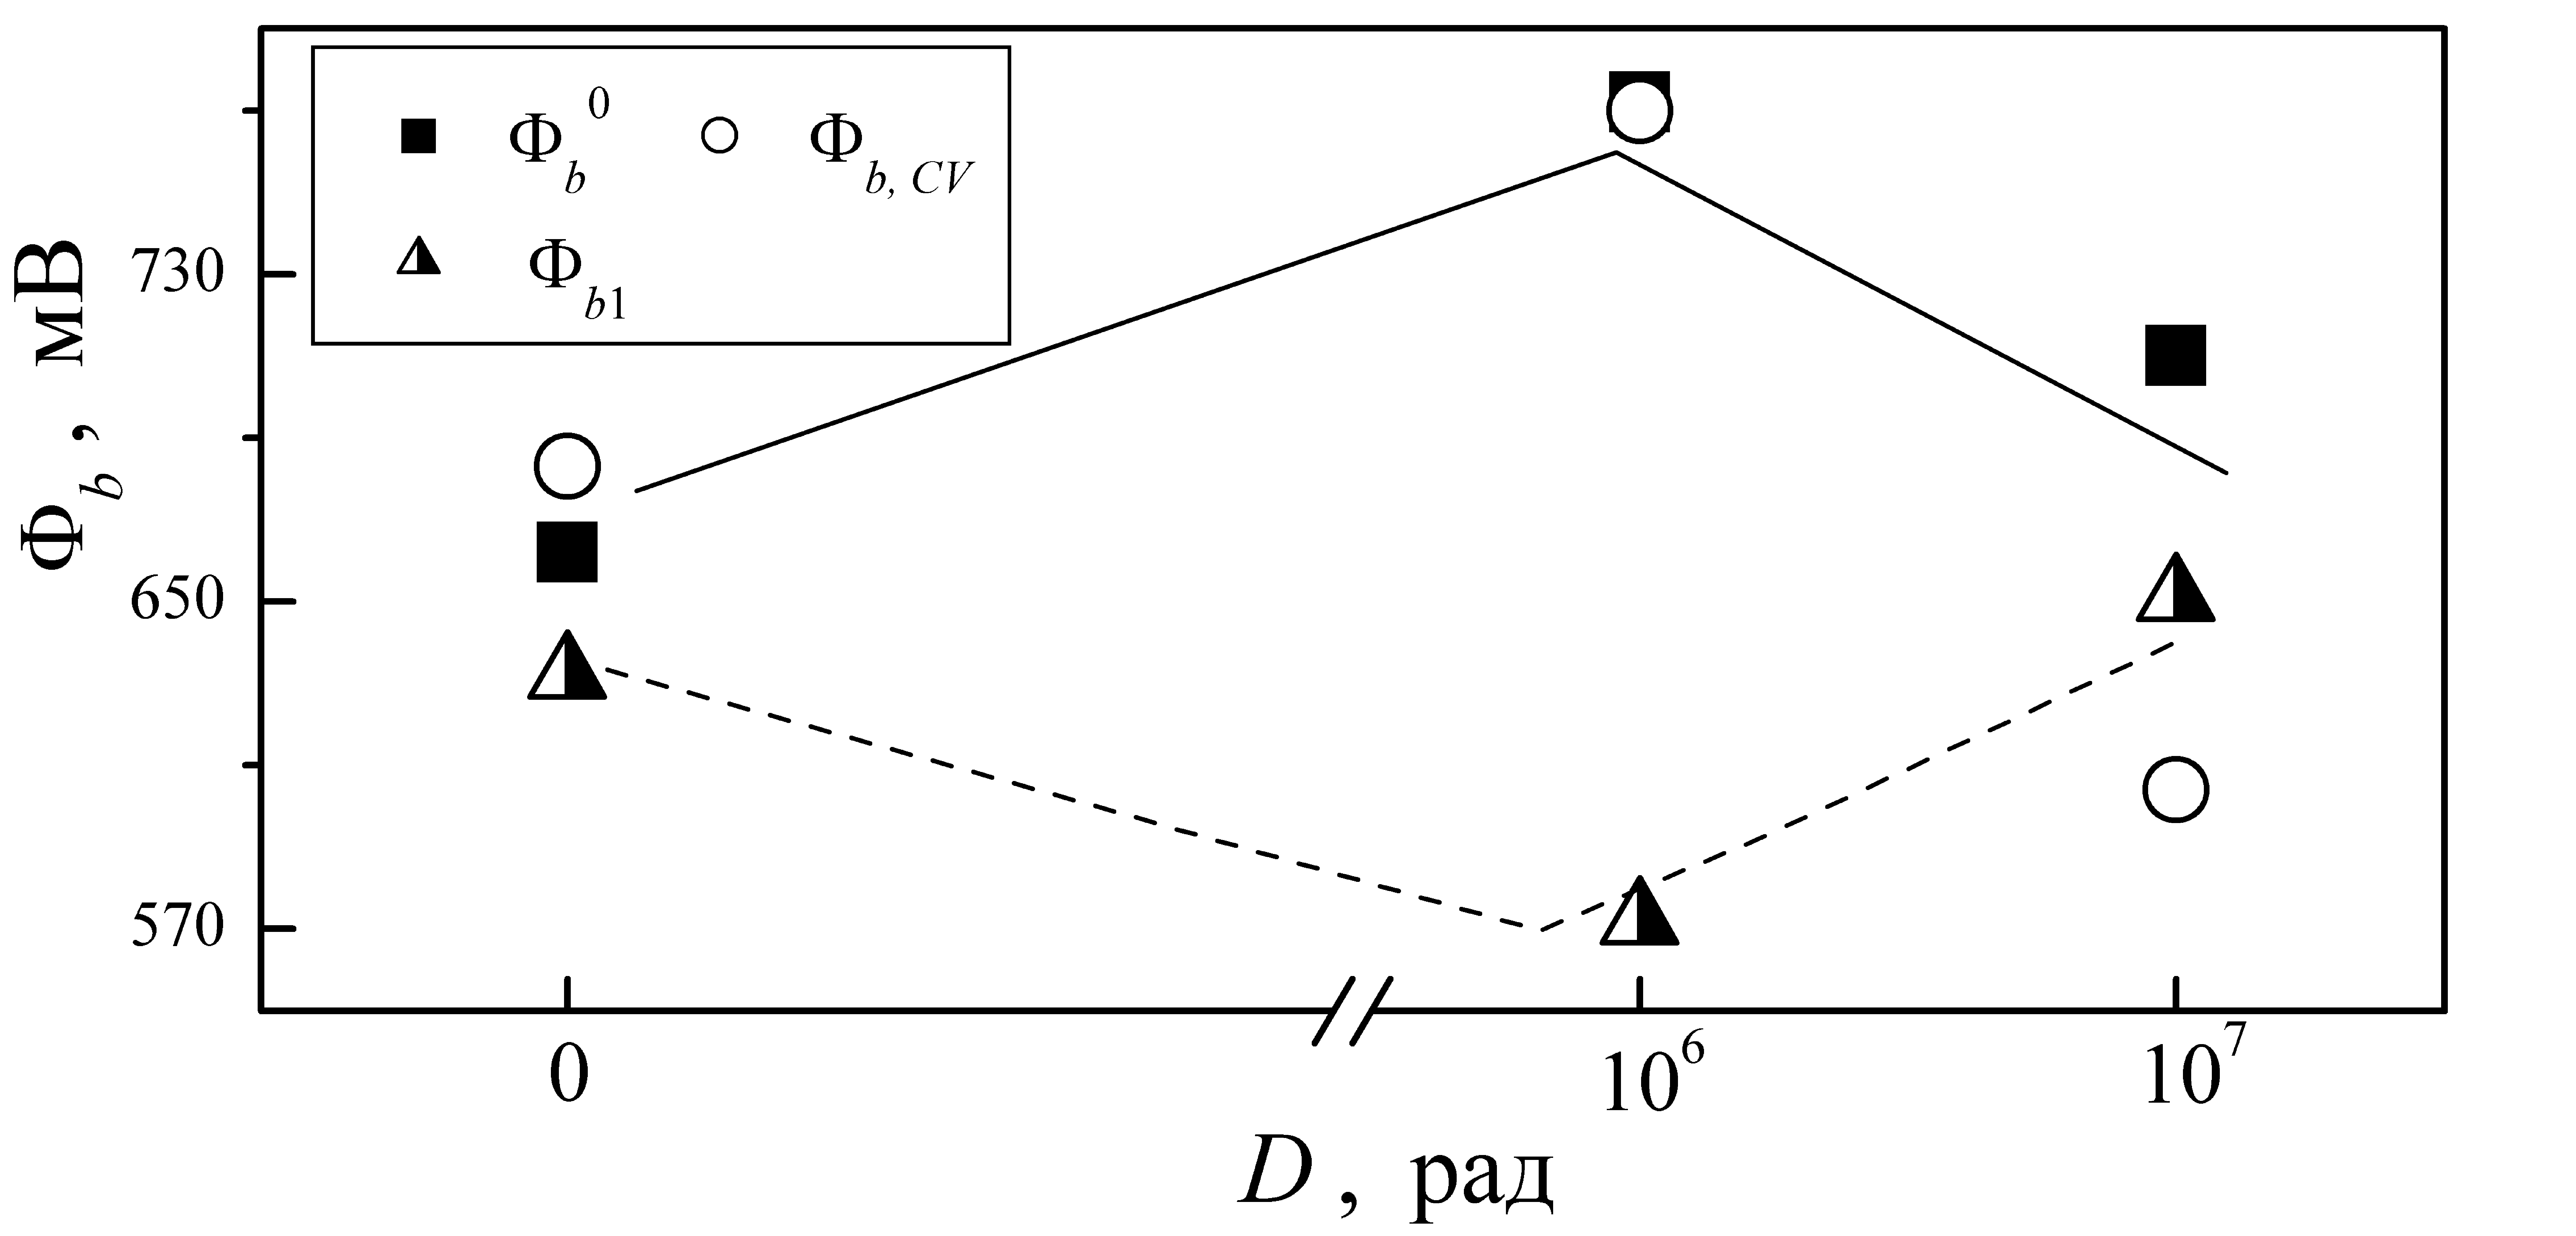
\includegraphics[width=0.8\textwidth]{figFbnonMon_SDA}
\caption{\label{figFbnonMon_SDA}
Дозові залежності ВБШ, визначені в рамках моделі неоднорідного контакту та безпосередньо з ВФХ та ВАХ.
$T=290$~К
}%
\end{figure}


З іншого боку, варто взяти до уваги, що згідно з даними табл.~\ref{tabSDAParRad},
$\Phi_b^0$ зростає після малих поглинутих доз $\gamma$--опромінення, тоді як подальше збільшення $D$ викликає зменшення
цієї величини.
Характер немонотонності збігається із виявленим раніше в роботах \cite{Karatas:2006NIMA, Vorobets, Pattabi} і суперечить
даним, отриманим безпосередньо з ВАХ (рис.~\ref{figFbnonMon_SDA})  та описаним в \cite{Umana,Verma}.
Отже, отримані результати показують, що тип немонотонності зміни висоти бар'єру Шотткі, який спостерігається
при збільшенні дози $\gamma$--опромінення,
залежить від ступеня неоднорідності контакту:
для однорідного інтерфейсу має спостерігатися перший варіант,
для структур із великим впливом патчів --- другий.

\begin{table}[b]
\caption{Параметри, визначені з ВАХ структур Al---$n$--$n^+$--Si в наближенні теорії DAT}
\label{tabSDAParRad:DAT}
\centering
\begin{tabular}{|l|c|c|c|}
\hline
$D$, рад &10$^6$ \textsuperscript{ a)}&10$^7$ \textsuperscript{ a)}&10$^7$ \textsuperscript{ б)}\\ \hline
Діапазон температур, K&120$\div$240&110$\div$130&110$\div$210\\
$E_{00}$, мВ&$17,8\pm0,5$&$23,5\pm0,5$&$80\pm10$\\
$\chi_\mathrm{calc}$, $10^{-3}$ K$^{-1}$&$39\pm3$&$26\pm2$&$8\pm1$\\
$\chi_\mathrm{fit}$, $10^{-3}$ K$^{-1}$&$73\pm6$&$42\pm4$&$8\pm1$\\
$I_{s0}$, $10^{-14}$A&$5\pm0,5$&$13\pm3$&$(17\pm2)\cdot10^{5}$\\
\hline
\multicolumn{4}{l}{\textsuperscript{ a)}\emph{для високотемпературної компоненти струму}}\\
\multicolumn{4}{l}{\textsuperscript{ б)}\emph{для низькотемпературної компоненти струму}}\\
\end{tabular}
\end{table}

Для з'ясування механізму перенесення заряду при низьких температурах
в опромінених структурах розглянемо температурні залежні фактора неідеальності --- рис.~\ref{figNTrad_SDA}.
Зауважимо, що спостерігаються немонотонні зміни $n_\mathrm{id}$ зі зростанням поглинутої дози.
Розглянуті результати підтверджують, що для g7SSDA доцільно застосовувати механізм ТЕ при $T>260$~К,
оскільки в цьому діапазоні температурна залежність $n_\mathrm{id}$ добре описується виразом (\ref{eqN_T:TE}) --- рис.~\ref{figNTrad_SDA}, крива 3.
Водночас з рисунку видно, що для ВТКС структури g6SSDA при $T<260$~К (крива 2), для ВТКС g7SSDA при $T<130$~К (крива 3) та для НТКС g7SSDA (крива 4)
зміни величини фактора неідеальності з підвищенням температури збігаються із передбаченими формулою (\ref{eqN_T:TFE}) з різними значеннями характеристичної
енергії, наведеними в табл.~\ref{tabSDAParRad:DAT}.
Це свідчить на користь наявності тунелювання носіїв заряду.
Зауважимо, що у випадку ТПЕ чи ПЕ величина характеристичної енергії має описуватися
виразом (\ref{eqE00:TFE}),
що для досліджених структур дає величину близько 2~меВ, яка набагато менше ніж визначені значення.
Крім того польова емісія характерна для температур, при яких $kT\approx E_{00}^\mathrm{TFE}$, що не відповідає дослідженому температурному
інтервалу.


\begin{figure}
\center
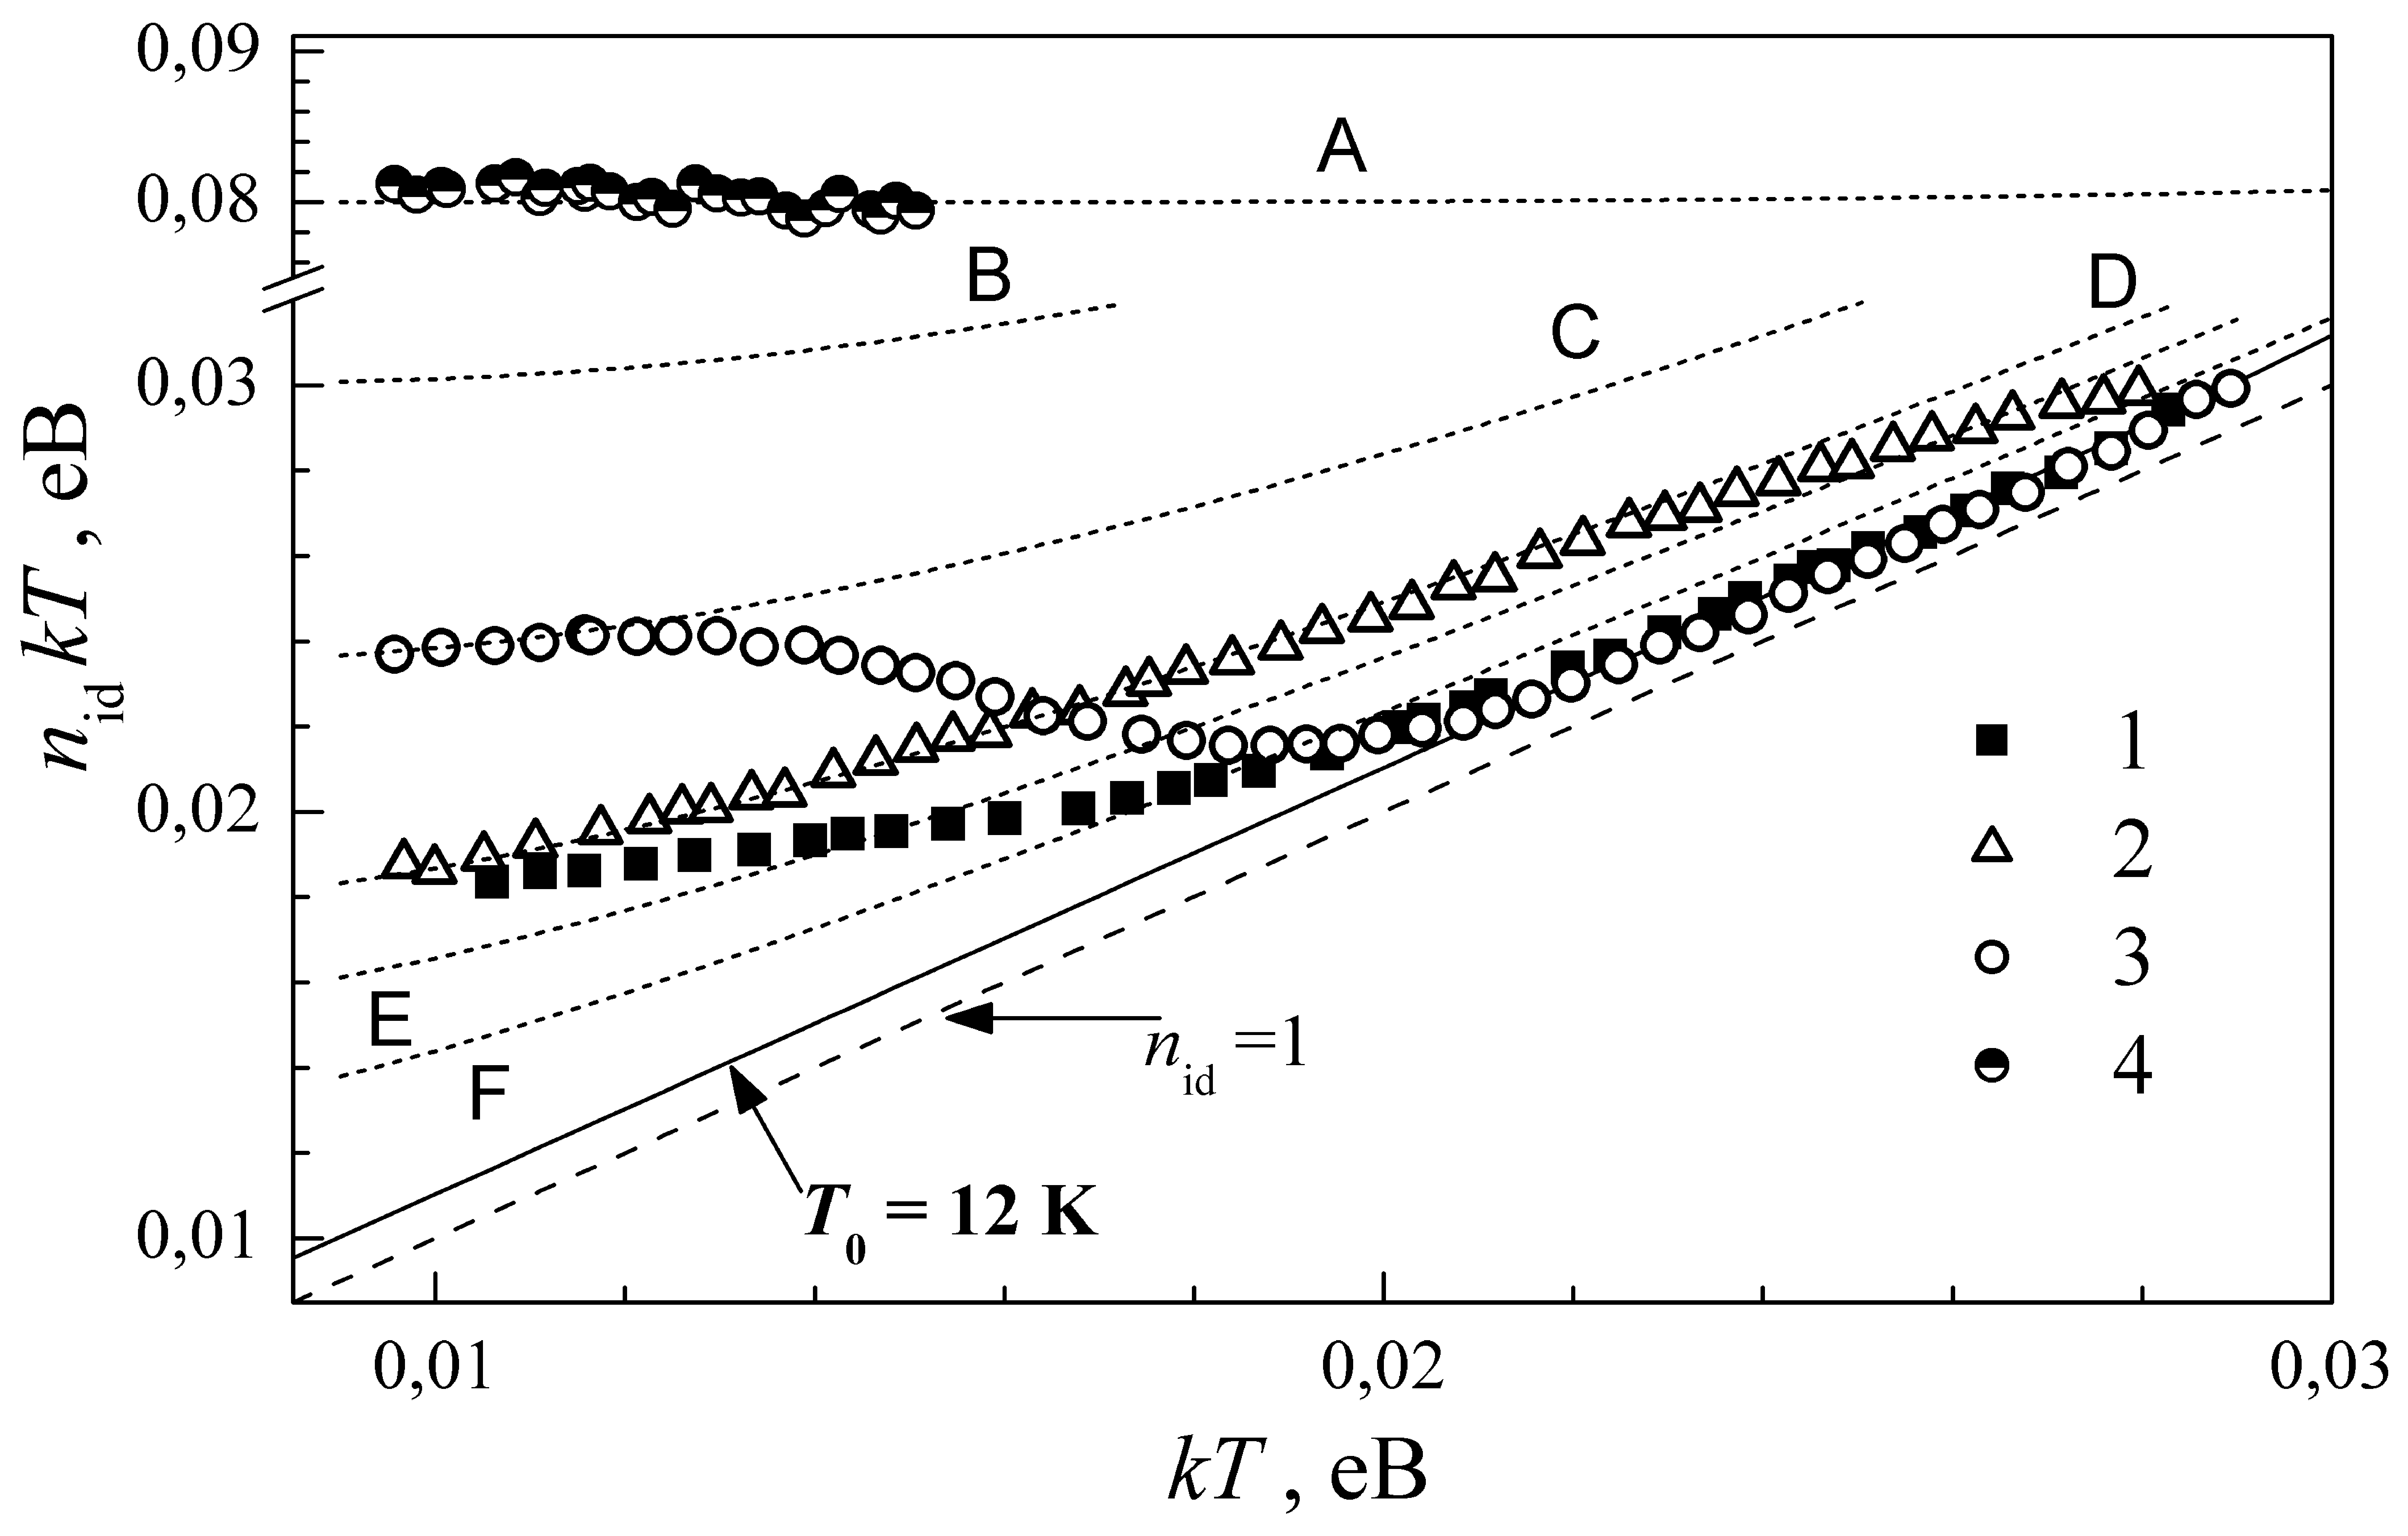
\includegraphics[width=0.75\textwidth]{figNTrad_SDA}
\caption{\label{figNTrad_SDA}
Температурна залежність оберненого нахилу ВАХ для ВТСК (1--3)
та НТСК (4).
$D$, рад: $0$ (1), $10^6$ (2), $10^7$ (3, 4).
Точки --- експеримент,
суцільна лінія розрахована відповідно до формули (\ref{eqN_T:TE}) з $T_0=12$~K,
пунктирні --- з використанням виразу (\ref{eqN_T:TFE}) при
$E_{00}$, меВ: 80 (A), 30 (B), 23.5 (C), 17.8 (D), 15 (E), 12 (F).
Штрихована лінія відповідає ідеальному випадку $n_{\mathrm{id}}=1$
}%
\end{figure}




При ТПЕ струм насичення через ДШ описується виразом \cite{Rhoderick1988, Roul}
\begin{equation}\label{eqIs:TFE}
  I_s=\frac{A^*T\sqrt{\pi{E_{00}}(\Phi_b^\mathrm{TFE}-V_n)}}{k\cosh\left(\frac{E_{00}}{kT}\right)}\cdot
  \exp\left[-\frac{V_n}{kT}-\frac{(\Phi_b^\mathrm{TFE}-V_n)}{n_{\mathrm{id}}^\mathrm{T}kT}\right]\,.
\end{equation}
На рис.~\ref{figFbTrad_SDA} (напівзаповнені трикутники) наведено температурну залежність $\Phi_b^\mathrm{TFE}$, отриману шляхом апроксимації ВАХ структур g6SSDA,
у припущенні, що струм проходить внаслідок ТПЕ.
Наведена залежність відрізняється від поведінки $E_g$.
Отже, ні термопольова, ні польова емісії не можуть бути причинами появи ні ВТКС, ні НТКС у досліджених структурах.

З іншого боку,  якщо перенесення заряду відбувається внаслідок багато--стрибкових DAT процесів, то струм насичення описується виразом \cite{Evstropov}:
\begin{eqnarray}
  I_s&=&I_{s0}\exp(\chi\,T) \label{eqIs:DAT}\,,\\
   \chi&=&\frac{\beta+k\ln(N_c/N_d)}{E_{00}}\,, \label{eqKsi:Dat}
\end{eqnarray}
де
$I_{s0}$ залежить, зокрема, від концентрації дефектів,
$\beta$ --- температурний коефіцієнт зниження $\Phi_b$.
На рис.~\ref{figIsTrad_SDA} наведено температурні залежності струмів насичення досліджених структур.
З рисунка видно, що між $\ln I_s$ та $T$ спостерігається лінійна залежність саме в тих температурних діапазонах,
де значення фактора неідеальності описується виразом, також характерним для DAT.


\begin{figure}
\center
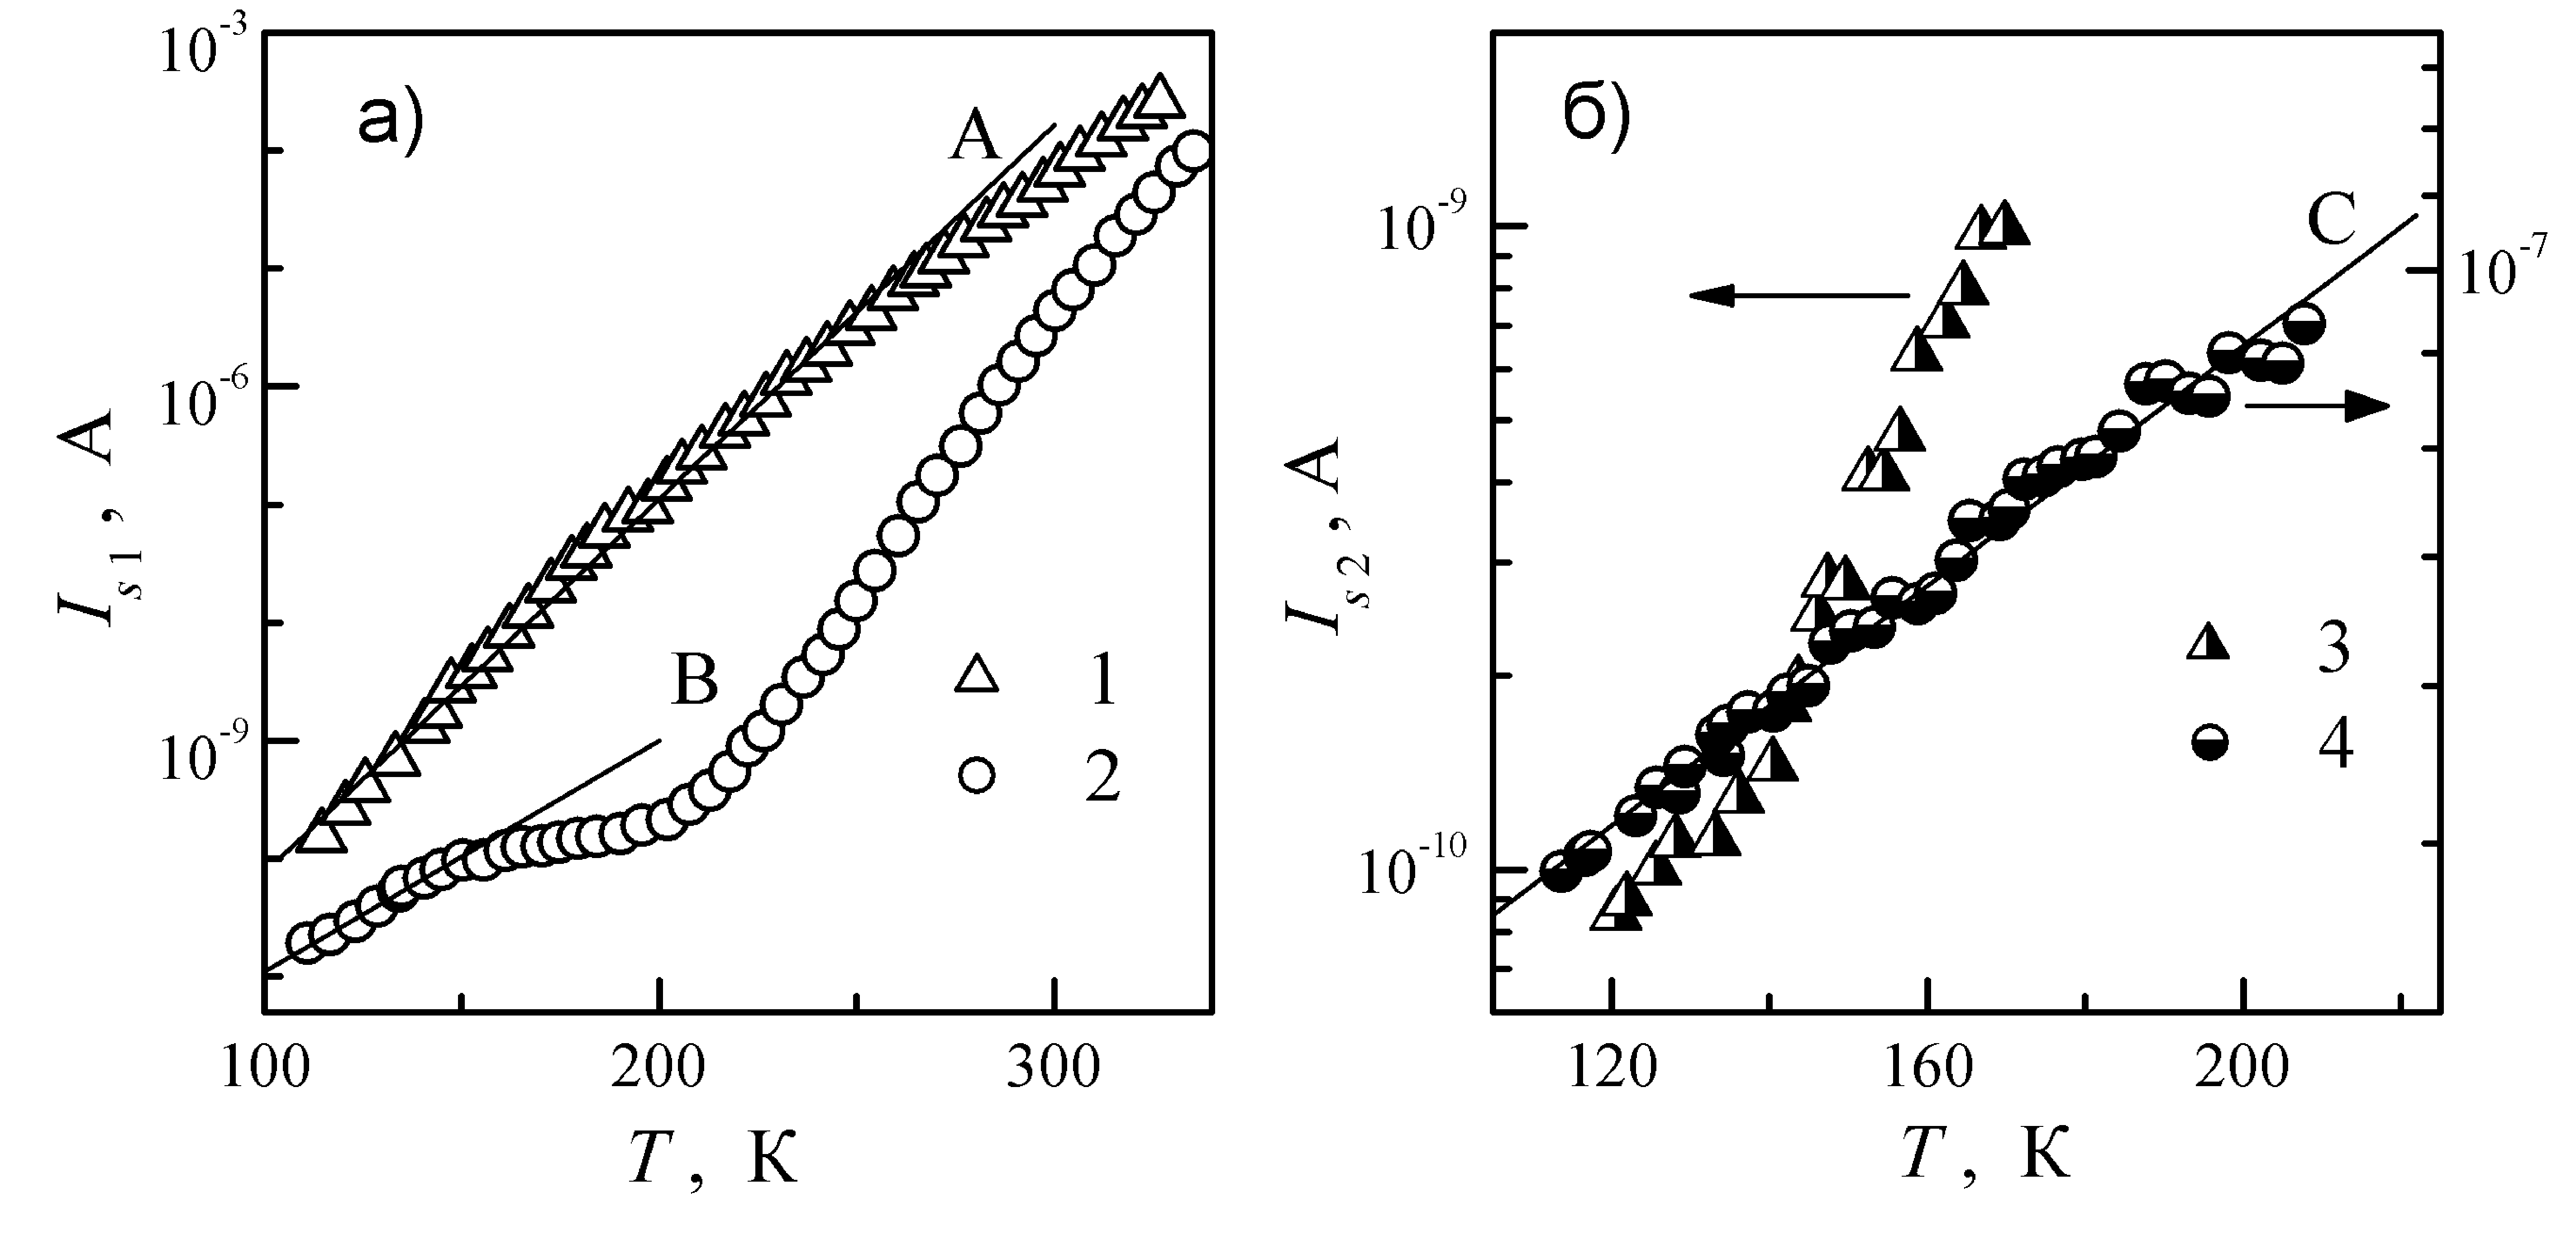
\includegraphics[width=0.95\textwidth]{figIsTrad_SDA}
\caption{\label{figIsTrad_SDA}
Температурні залежності струму насичення ВТКС (а, незаповнені точки)
та НТКС (б, напівзаповнені точки).
$D$, рад: 10$^6$~(1, 3, трикутники), 10$^7$~(2, 4, кола).
Лінії розраховані за формулою (\ref{eqIs:DAT}).
$\chi$, $10^{-3}$~K$^{-1}$: 73~(A), 42~(B), 26~(C).
$I_s$, A: $5\cdot10^{-14}$~(A),
$1,3\cdot10^{-13}$~(B),
$1,7\cdot10^{-8}$~(C)
}%
\end{figure}

Використовуючи вираз (\ref{eqKsi:Dat}), значення $\beta=0,26$~меВ/K \cite{Aboelfotoh, Evstropov} та величини $E_{00}$,
отримані із залежностей $n_\mathrm{id}=f(T)$ (рис.~\ref{figNTrad_SDA}),
були розраховані значення $\chi_\mathrm{calc}$ для g6SSDA та g7SSDA, наведені в табл.~\ref{tabSDAParRad:DAT}.
Ця таблиця також містить величини $\chi_\mathrm{fit}$, отримані шляхом апроксимації залежностей $I_s$ з використанням виразу~(\ref{eqIs:DAT}).
Як видно з наведених даних, величини, отримані різними способами, не дуже суттєво відрізняються одна від одної.
Цей збіг, а також температурні залежності $I_s$ та $n_\mathrm{id}$ свідчать,
що ВТКС в g6SSDA при $T=120\div240$~K, ВТКС в g7SSDA при $T<130$~K і НТКС в g7SSDA визначаються процесами багато--стрибкового DAT.






\subsection{Перенесення заряду в $\gamma$--опромінених структурах Al---$n$--$n^+$--Si при зворотному зміщенні}

\begin{figure}
\center
\includegraphics[width=0.65\textwidth]{figIV_SDArRad}
\caption{\label{figIV_SDArRad}
Зворотні характеристики структур SSDA при температурах 130~K (незаповнені точки)
та 330~K (напівзаповнені точки).
$D$, рад: 0 (квадрати), $10^6$ (трикутники), $10^7$ (кола)
}%
\end{figure}

Приклади зворотних ВАХ досліджуваних структур при низьких та високих температурах наведено на рис.~\ref{figIV_SDArRad}.
Видно, що $\gamma$--опромінення з $D=10^6$~рад
\begin{enumerate}[label=\asbuk*),leftmargin=0em,itemindent=1.5em]
\item залишає майже незмінною величину зворотного струму поблизу азотних температур;
\item у декілька разів підвищує величину $I_R$ в околі кімнатних температур;
\item практично не впливає на польову залежність зворотного струму.
\end{enumerate}
Зі збільшенням поглинутої дози при малих зміщеннях спостерігається збільшення струму при низьких температурах і протилежний ефект при високих;
водночас при $V_R>2$~В струм практично перестає залежати від температури, зростаючи при цьому приблизно на порядок 
порівняно з вихідними зразками.




Проведений аналіз показав, що вираз (\ref{eqIr}), який використовувався для опису зворотних гілок ВАХ неопромінених структур,
не може з достатньою точністю відтворити температурну та польову залежності $I_R$ в Al---$n$--$n^+$--Si після опромінення.
Для апроксимації даних використовувався наступний вираз:
\begin{eqnarray}
\label{eqIrRad}
I_R(T,V_R)&=&C_\mathrm{TE}(V_R)T^2\exp\left[-\frac{E_\mathrm{TE}(V_R)}{kT}\right]+I_\mathrm{FN}(V_R)+I_\mathrm{MPT}(T,V_R)\,,
\end{eqnarray}
де
перші два доданки, як і раніше,
пов'язані з ТЕ та температуро--незалежною компонентами зворотного струму,
а третій залежить як від $T$, так і від $V_R$ та описує шлях перенесення заряду, який виник внаслідок опромінення.

Як і для неопромінених структур,
величина $E_{TE}$ залежить від зміщення, проте для g6SSDA та g7SSDA характеристична енергія лінійно залежить від $V_{bb}^{1/4}$
 --- рис.~\ref{figIrTErad_SDA}.
Це є свідченням, що у цьому випадку вплив неоднорідностей
на термоемісійний зворотній струм менш суттєвий, а польове зниження ВБШ пов’язане з дією сил зображення \cite{Rhoderick1988,Andrews}.

\begin{figure}
\center
\includegraphics[width=0.65\textwidth]{figIrTErad_SDA}
\caption{\label{figIrTErad_SDA}
Польові залежності характеристичної енергії ТЕ складової зворотного струму структур g6SSDA (трикутники) та g7SSDA (кола).
Точки --- експеримент, прямі --- лінійна апроксимація за методом найменших квадратів
}%
\end{figure}

Температуро--незалежна компонента $I_\mathrm{FN}$ незалежно від дози опромінення має тунельний характер --- див. рис.~\ref{figIrFNrad_SDA},
причому її нахил у координатах Фаулера--Нордгейма однаковий.
Згідно з (\ref{eqFowlNord}) та (\ref{eqFN:Et}) це свідчить, що тунелювання відбувається через один і той самий дефектний рівень $E_c-E_t=120$~меВ.
З іншого боку,
зсув залежності $I_\mathrm{FN}/F_m^2=f(F_m^{-1})$ відображає збільшення концентрації відповідних дефектів, яка
особливо помітна для g7SSDA.
Це додатково свідчить, що $I_\mathrm{FN}$ зумовлена тунелюванням за участю рівнів міжвузлового атому вуглецю С$_i$,
який є вторинним дефектом при опроміненні кремнію $\gamma$--квантами $^{60}$Со \cite{Vavilov1990r}.
Оскільки в наших експериментах температура досягала 330 К, необхідно зауважити, що в роботі \cite{Song1987} показана можливість відпалу С$_i$
 в об’ємному кремнії при температурах 300$\div$350~К шляхом утворення комплексу з міжвузловим атомом кисню чи заміщуючим атомом вуглецю.
Виявлена стабільність С$_i$ у досліджених структурах може бути викликана процесами просторового розділення різнойменно--заряджених дефектів, які раніше виявлені при $\gamma$--опроміненні бар’єрних структур \cite{Muzafarova}.
Отже, струм $I_\mathrm{FN}$ може бути зумовлений прямим  тунелюванням за участю рівня С$_i$.



\begin{figure}
\center
\includegraphics[width=0.6\textwidth]{figIrFNrad_SDA}
\caption{\label{figIrFNrad_SDA}
Залежність температуро--незалежної компоненти зворотного струму
структур SSDA (квадрати), g6SSDA (трикутники) та g7SSDA (кола)
у координатах Фаулера--Нордгейма.
Точки --- експеримент, пряма --- лінійна апроксимація% за методом найменших квадратів
}%
\end{figure}


Струм $I_\mathrm{MPT}$, який спостерігається лише в опромінених структурах, зростає з підвищенням поглинутої дози.
Поява нового механізму перенесення заряду після $\gamma$--опромінення є відомим ефектом \cite{Gullu:2008,Karatas:2005NIMA}.
%;
%наприклад, згідно з результатами \cite{Gullu:2008,Karatas:2005NIMA} причинами додаткового струму можуть бути генераційно--рекомбінаційні процеси або
%тунелювання.
З літератури \cite{Bulyarskii2001r,Evstropov,Ganichev:2000} відомо, що у структурах МН може протікати струм,
пов’язаний з тунельною багатофононною іонізацією глибоких домішкових центрів.
При цьому для кожної температури існує діапазон полів (загалом тим більший, чим вища температура), коли імовірність багатофононної іонізації $P$
та величина струму експоненційно зростають із підвищенням напруженості електричного поля $F_m$ \cite{Bulyarskii2001r,Ganichev1997,Ganichev:2000}:
$P(F_m,\,T)=P(0,\,T) \exp(F_m^2/F_0^2)$,
де $F_0$ --- деяке характеристичне значення напруженості.
Саме така залежність спостерігається для $I_\mathrm{MPT}$ (рис.~\ref{figIrPATrad_SDA}).
 Показано \cite{Bulyarskii2001r,Ganichev1997,Ganichev:2000}, що коефіцієнт нахилу $F_0$ має залежати від температури:

\begin{equation}\label{eqPAT}
    F_0^{\,-2/3}=\left[\frac{d(\ln I_\mathrm{MPT})}{d(F_m^2)}\right]^{1/3}\propto \sqrt[3]{\frac{q^2\hbar^2}{24k^3m^*}}\,\frac{1}{T}\,.
\end{equation}

\begin{figure}
\center
\includegraphics[width=0.55\textwidth]{figIrPATrad_SDA}
\caption{\label{figIrPATrad_SDA}
Польові залежності компоненти зворотного струму $I_\mathrm{MPT}$ 
%при різних температурах 
для структури g7SSDA.
Точки --- експеримент, пряма --- лінійна апроксимація %за методом найменших квадратів
}%
\end{figure}



Нахил залежності $\ln I_\mathrm{MPT}\sim F^2$ дійсно є лінійною функцією оберненої температури (рис.~\ref{figIrPATF0rad_SDA}).
Значення, отримані шляхом лінійної апроксимації даних на рис.~\ref{figIrPATF0rad_SDA}
($2,9\cdot10^{-3}$ та $0,6\cdot10^{-3}$~K$\cdot$м$^{2/3}$$\cdot$В$^{-2/3}$ для g6SSDA та g7SSDA, відповідно)
цілком задовільно узгоджуються з теоретичним значенням
$q^2\hbar^2/(24k^3m^*)=1,7\cdot10^{-3}$~K$\cdot$м$^{2/3}$$\cdot$В$^{-2/3}$.
Отже, додаткова складова зворотного струму зумовлена
процесами багатофононної іонізації в області просторового заряду за участю рівнів радіаційних дефектів.
%
%
%поява радіаційних дефектів та пов’язаних із ними рівнів у забороненій зоні,
%за участю яких і відбуваються процеси багатофононної іонізації в області просторового заряду.



\begin{figure}
\center
\includegraphics[width=0.55\textwidth]{figIrPATF0rad_SDA}
\caption{\label{figIrPATF0rad_SDA}
Температурна залежність коефіцієнта нахилу польової залежності компоненти зворотного струму $I_\mathrm{MPT}$.
Точки --- експеримент, прямі --- лінійна апроксимація за методом найменших квадратів
}%
\end{figure}

На рис.~\ref{figeIrRad_SDA} показані температурні залежності відносних внесків $\nu_\mathrm{TE}$, $\nu_\mathrm{FN}$ та $\nu_\mathrm{MPT}$
кожної з компонент у загальний зворотний струм, розраховані аналогічно до виразів, наведених на с.~\pageref{nu_IR} при певних значеннях $V_R$.
Видно, що
\begin{enumerate}[label=\asbuk*),leftmargin=0em,itemindent=1.5em]
\item струм $I_\mathrm{FN}$ є найбільшим у g7SSDA і  переважає при низьких температурах;
% і його внесок зменшується при зростанні $T$;
\item у g6SSDA тунельний струм перевищує ТЕ складову при $T<250$~K, що збігається з результатами, отриманими при аналізі прямого струму;
\item у g7SSDA внесок $I_\mathrm{TE}$ стає переважаючим лише при $T>300$~K, тоді як при нижчих температурах домінюючою є температуро--незалежна компонента.
\end{enumerate}

\begin{figure}
\center
\includegraphics[width=0.7\textwidth]{figeIrRad_SDA}
\caption{\label{figeIrRad_SDA}
Температурні залежності відносних внесків у зворотний струм
структур g6SSDA (a) та g7SSDA (б)
при $V_R=0,5$~В та $V_R=3$~В
}%
\end{figure}

Зазначимо, що останній факт разом зі слабкою температурною залежністю струму насичення ВТКС у g7SSDA при $T=150\div220$~K (рис.~\ref{figIsTrad_SDA},а, крива 2)
доводить, що в цьому температурному діапазоні тунелювання є основним механізмом перенесення заряду і при прямому зміщенні.
Відомо \cite{Yu}, що наявність тунельної компоненти є причиною помилок у визначенні $A^*$ та ВБШ за допомогою залежності Річардсона.
На нашу думку, вплив тунелювання залишається достатньо суттєвим для g7SSDA і в інтервалі температур 260$\div$330~K і саме це є причиною
відмінності отриманого значення сталої Річардсона (табл.~\ref{tabSDAParRad}) та відомого з літератури, а також перевищення $\Phi_b^0$ величини $\Phi_{b,CV}$.

Узагальнюючи картину змін параметрів структур Al---$n$--$n^+$--Si внаслідок опромінення $\gamma$--квантами $^{60}$Co, зауважимо наступне.
До опромінення перенесення заряду при прямому зміщенні у всьому дослідженому інтервалі температур відбувалося внаслідок ТЕ через неоднорідний бар'єр,
причому при $T>230$~K середня висота бар'єру $\Phi_b^0=0,663$~В, а стандартне відхилення $\sigma_{\Phi0}=0,04$~В.
Після того, як поглинута доза досягла $10^6$~рад, домінуючим механізмом перенесення заряду в діапазоні температур
$120\div240$~K як при прямому зміщенні, так і при зворотному стає DAT із характеристичною енергією $E_{00}=17,8$~меВ.
Це зумовлено появою у збідненому прошарку РД, зокрема міжвузлових атомів вуглецю, які спричинюють збільшення
концентрації рівнів у забороненій зоні, і, отже, інтенсифікацію процесів тунелювання, у тому числі і багатофононного.
При $T>260$~K основним механізмом залишається термоелектронна емісія через неоднорідний бар'єр, проте значення $\Phi_b^0$ та $\sigma_{\Phi0}$
зростають до 0,772~В та 0,1~В, відповідно.
Аналіз НТКС показав, що поява додаткового струму, як і для неопромінених структур, зумовлена ефективним проходженням носіїв через області зниженого бар'єру,
причому загальна площа патчів не змінилась, проте зросла висота бар'єру (з 54 до 74~мВ).
Тобто відбуваються радіаційно--індуковані процеси зміни як характеристик області поза межами патчів, так і самих неоднорідностей.
Причиною зміни середнього значення ВБШ та $\Phi_{b,p}$ може бути накопичення на інтерфейсній межі структур МН
радіаційних дефектів акцепторного типу.
Зауважимо, що ефекти просторового розділення $\gamma$--індукованих точкових дефектів із протилежним зарядом внаслідок дії пружних полів
у бар'єрних структурах достатньо широко відомі в літературі \cite{Shcherb, Muzafarova}.
Щодо збільшення $\sigma_{\Phi0}$, то зазначимо, що можливою причиною появи патчів вважаються дислокації \cite{GELCZUK2014}.
У приповерхневих шарах Si структур Al---$n$--$n^+$--Si, ідентичних дослідженим, виявлено скупчення дислокацій та дефекти пакування \cite{VOROBETS2005,Vorobets},
що є додатковим аргументом на користь того, що причиною появи областей неоднорідності ВБШ є самі ці протяжні дефекти.
З іншого боку відомо, що утворені в процесі опроміненні вільні носії можуть захоплюватись на дефекти пакування та бути причиною
полегшення руху дислокацій --- явище так званого радіаційно--підсиленого дислокаційного ковзання (REDG, radiation--enhanced dislocation glide) \cite{REDG}.
Тобто в нашому випадку $\gamma$--опромінення викликає переміщення протяжних дефектів та їхнє часткове перегрупування з утворенням скупчень більшого розміру.
Ефекти зменшення загальної кількості таких дефектів внаслідок лазерного опромінення спостерігалися і раніше в роботах \cite{VOROBETS2005,Vorobets}.
У рамках моделі неоднорідного контакту (див. формули (\ref{eqGigFSigG}) та (\ref{eqGammaP})), збільшення розкиду розмірів патчів має спричинити зростання $\sigma_{\Phi0}$.
Збільшення впливу патчів маскує зростання ВБШ за їхніми межами і викликає зменшення ефективної висоти бар'єру, яка визначається безпосередньо з ВАХ.

При збільшенні дози до $10^7$~рад концентрація РД суттєво зростає --- див., наприклад табл.~\ref{tabDefectNt}, де представлені результати оцінки дефектоутворення
у кристалах кремнію при таких же дозах $\gamma$--опроміненням, які використовувалися для модифікації
структур SSDA.
Відомо \cite{Boltovets}, що в ДШ релаксація механічних напруг може відбуватися внаслідок гетерування ТД.
Ймовірно, у досліджених структурах такими центрами гетерування є саме патчі.
Як наслідок накопичення ними від'ємно заряджених дефектів (як радіаційних, так і тих, що збільшили рухливість внаслідок іонізації) характер перенесення заряду через ці області змінився з термоемісійного на тунельний.
Тобто патчі почали виконувати роль тунельних шунтів і перестали впливати на ТЕ процеси.
Відтак,
а)~НТКС при прямому зміщенні суттєво зросла, причому перенесення заряду почало відбуватися завдяки процесам DAT із $E_{00}=80$~меВ;
б)~тунельний струм став основним не лише при зворотному зміщенні практично у всьому дослідженому температурному інтервалі,
але й при прямому зміщенні при $T=(150\div220)$~K;
в)~прямий струм при $T=260\div330$~K, в основному, визначається ТЕ процесами через бар'єр висотою близько 710~мВ,
проте вплив тунелювання у цьому температурному діапазоні не може бути знехтуваний;
г)~ефективна ВБШ, яка визначається безпосередньо з ВАХ, збільшилась порівняно з  $D=10^6$~рад, на противагу реальному зменшенню висоти бар'єру в однорідній області внаслідок гетерування дефектів акцепторного типу.

Необхідно зауважити, що зі збільшенням поглинутої дози $\gamma$--квантів $^{60}$Co спостерігалися ефекти як немонотонної зміни механічних напруг
в епітаксійних плівках, так і зміни заряду радіаційних дефектів, накопичених на межі розділу \cite{Muzafarova, Belyaev}.
Ці явища також є непрямим доказом на користь запропонованого механізму радіаційно--індукованої перебудови кремнієвих діодів Шотткі.



\section{Вплив ультразвукового навантаження на перенесення заряду в $\gamma$--опромінених та неопромінених структурах Al---$n$--$n^+$--Si\label{MSSi_USL}}

\subsection{Режими ультразвукового навантаження структур Al---$n$--$n^+$--Si}

Схема акустичного навантаження структур Al---$n$--$n^+$--Si наведено на рис.~\ref{figUSL},б.
%рис.~\ref{figUSL:SDA}.
%Відмінність від схеми, зображеної на рис.~\ref{figUSL:SC}, полягає у наявності діелектричного прошарку,
%необхідного для електричної розв'язки при вимірюванні ВАХ.
Для оцінки параметрів ультразвукового навантаження використовувалися формули (\labelcref{eqAmpUS,eqWus,eqM0,eqDefUS}) та дані табл.~\ref{tabLNO}.
При досліджені АІ ефектів у зразках збуджувалися повздовжні хвилі.
УЗН відбувалось при температурах, близьких до  кімнатної.
Параметри УЗН структур Al---$n$--$n^+$--Si, їхнє позначення та зразки, до яких вони застосовувалися, наведено в табл.~\ref{tabUSL:SD}.

%\begin{figure}%[b]
%\center
%\includegraphics[width=0.4\textwidth]{USL_SDA}%
%\caption{\label{figUSL:SDA}
%Використані схеми УЗН.
%1 --  екран (алюмінієва фольга, товщина 0,012 мм);
%2 --- п'єзоелектричний перетворювач (LiNbO$_3$);
%3 --- діелектричний прошарок (слюда, товщина 0,03 мм);
%4 --- контакти для вимірювання ВАХ;
%5 --- контакти для збудження УЗ
%}
%\end{figure}


\begin{table}
\caption{\label{tabUSL:SD}Параметри ультразвукових навантажень структур Al---$n$--$n^+$--Si
}
\center
\begin{tabular}{|c|c|c|c|c|c|c|c|}
\hline
$f_\mathtt{US}$,&Тип&$W_{\mathtt{US}}$,&$\xi_{\mathtt{US}}$,&$u_{\mathtt{US}}$,&$T$,&УЗН&Зразок\\
МГц&хвиль&Вт/см$^2$&$10^{-6}$&нм&K&&\\
\hline
9,6&повздовжні&до 0,66&до 3,1&до 0,43&$\sim$305&U10SD&SSDA\\ \hline
30,1&повздовжні&до 0,42&до 2,5&до 0,11&$\sim$305&U30SD&SSDA\\ \hline
9,6&повздовжні&до 1,3&до 4,3&до 0,60&$\sim$305&U10g6SD&g6SSDA\\ \hline
9,6&повздовжні&до 1,1&до 4,0&до 0,56&$\sim$305&U10g7SD&g7SSDA\\ \hline
\end{tabular}
\end{table}


\subsection{Акусто--індуковані зміни висоти бар'єру Шотткі}
\begin{figure}[b]
\center
\includegraphics[width=0.6\textwidth]{figIVUSL_SDA}
\caption{\label{figIVUSL_SDA}
Прямі  ВАХ  структур SSDA (квадрати), g6SSDA (трикутники) та g7SSDA (кола), виміряні при $T=305$~K.
Заповнені та порожні точки відповідають вимірам при УЗН та без нього, відповідно.
$W_\mathtt{US}$, Вт/см$^2$: 0,7 (SSDA), 1,3 (g6SSDA), 1,1 (g7SSDA).
%Лінії --- апроксимація відповідно до формули (\ref{eqSDA_IV})
}%
\end{figure}

\begin{figure}
\center
\includegraphics[width=0.7\textwidth]{figFbUSL_SDA}
\caption{\label{figFbUSL_SDA}
Залежності висоти бар'єру Шотткі (а) та фактора неідеальності (б)  від інтенсивності УЗ для
структур SSDA (квадрати, ліві вертикальні осі), g6SSDA (трикутники, ліві осі) та g7SSDA (кола, праві осі).
$T=305$~K.
%$f_\mathtt{US}$, МГц: 9,6 (SSDA, g6SSDA, g7SSDA), 30,1 (SSDA).
Горизонтальні пунктирні лінії відповідають значенням параметрів, виміряних без УЗН
}%
\end{figure}

На рис.~\ref{figIVUSL_SDA} показано прямі гілки ВАХ структур Al---$n$--$n^+$--Si, виміряні при УЗН та для акустично ненавантажених
зразків при однакових температурах.
З рисунка видно, що внаслідок дії УЗ прямий струм зростає, причому
ефективність АІ збільшення залежить як від величини напруги зміщення, так і від ступеню опромінення.
Після припинення УЗН, вольт-амперні характеристики відновлювалися, що свідчить про оборотність акусто--індукованих змін.



За методикою, стандартною для даного розділу,  визначені характеристики ДШ в умовах поширення акустичних коливань різної інтенсивності.
Зауважимо, що оскільки температура УЗН близька до кімнатної, то внесок НТКС знехтувано малий.
АІ зміни ВБШ та фактора неідеальності представлена на рис.~\ref{figFbUSL_SDA}.
Дані на рисунку дозволяють виділити наступні особливості  впливу УЗ на характеристики структури метал---кремній:
\begin{enumerate}[label=\asbuk*),leftmargin=0em,itemindent=1.5em]
\item УЗН викликає зменшення ВБШ;

\item залежність $\Delta\Phi_b(W_\mathtt{US})$ 
%зміни висоти бар'єру від $W_\mathtt{US}$ 
у неопромінених структурах має пороговий характер:
     величина $\Phi_b$ залишається практично незмінною поки \mbox{$W_\mathtt{US}<0,4$~Вт/см$^2$}, після чого
    зменшення ВБШ досягає $(13\pm4)$~мВ при $W_\mathtt{US}\simeq0,7$~Вт/см$^2$;

\item %на відміну від ефектів, виявлених при розгляді АДВ у КСЕ (параграфи \ref{sbNIsc} та \ref{sBulyrMethod}),
 при збільшенні $f_\mathtt{US}$ підвищення ефективності впливу УЗН не спостерігається;

\item після $\gamma$--опромінення ефективність впливу УЗН на ВБШ знижується:
абсолютне значення $\Delta\Phi_b$ не перевищує $10$~мВ для g7SSDA та $3$~мв  для g6SSDA;
% при $W_\mathtt{US}>1$~Вт/см$^2$;

\item на залежності $\Phi_b$ від $W_\mathtt{US}$ для опромінених структур поріг не спостерігається;

\item збільшення дози призводить до підсилення ефективності АІ змін ВБШ;

\item незначні АІ зміни фактора неідеальності спостерігаються у випадку, коли $n_\mathtt{id}>1,1$ (зразок g6SSDA);
    у випадку, коли $n_\mathtt{id}$ близький до одиниці, в умовах УЗН його величина практично не міняється (зразки SSDA та g7SSDA).
\end{enumerate}



Згідно з (\ref{eqFb0T}) причиною АІ змін ВБШ може бути вплив УЗ на $\Phi_b^0$ або на $\sigma_{\Phi0}$ (або й, звичайно, на обидві величини).
У свою чергу, рівняння  (\ref{eqN_T:TE}), (\ref{eqFb0T}) та (\ref{eqN_T0}) дозволяють оцінити, яким чином повинен був би змінюватись фактор неідеальності,
якби причиною зміни ВБШ були б зміни лише одного параметра з пари $(\Phi_b^0;\:\sigma_{\Phi0})$ , тоді як інший залишається постійним.
Дійсно, при $\Phi_b^0=const$
\begin{eqnarray*}
  \Delta \Phi_b (\Phi_b^0=const)&=& \Phi_{b,in}-\Phi_{b,\mathtt{US}}=\Phi_b^0-\frac{q\sigma^2_{\Phi0,in}}{2kT}-\Phi_b^0+\frac{q\sigma^2_{\Phi0,\mathtt{US}}}{2kT}= \\
   &=&\frac{q\left(\sigma^2_{\Phi0,\mathtt{US}}-\sigma^2_{\Phi0,in}\right)}{2kT}, \\
   V_{bb,in}&=&V_{bb,\mathtt{US}},\\
%\end{eqnarray*}
%\begin{eqnarray*}
  \Delta n_{\mathrm{id}} (\Phi_b^0=const)&=&1+\frac{q\sigma_{\Phi0,in}^2}{3kV_{bb}T}-1-\frac{q\sigma_{\Phi0,\mathtt{US}}^2}{3kV_{bb}T}=\\
  &=&\frac{q\left(\sigma^2_{\Phi0,in}-\sigma^2_{\Phi0,\mathtt{US}}\right)}{3kV_{bb}T}=-\frac{2\Delta \Phi_b}{3V_{bb}}.
\end{eqnarray*}

Якщо ж незмінним залишається стандартне відхилення висоти бар'єру, то
\begin{eqnarray*}
  \Delta \Phi_b (\sigma_{\Phi0}=const)&=&\Phi_{b,in}^0-\Phi_{b,\mathtt{US}}^0,\\
  V_{bb,in}-V_{bb,\mathtt{US}}&=&\Delta \Phi_b,\\
%\end{eqnarray*}
%\begin{eqnarray*}
  \Delta n_{\mathrm{id}} (\sigma_{\Phi0}=const)&=&\frac{q\sigma_{\Phi0}^2}{3kV_{bb,in}T}-\frac{q\sigma_{\Phi0}^2}{3kV_{bb,\mathtt{US}}T}=\\
  &=&-\frac{q\sigma_{\Phi0}^2\Delta \Phi_b}{3kT\,V_{bb,in}(V_{bb,in}-\Delta \Phi_b)}.
\end{eqnarray*}
Розрахунки, проведені з використанням величини $\Delta \Phi_b=0,013$~мВ (випадок U10SD, максимальна інтенсивність) та даних табл.~\ref{tabPar:SSDA},
показують, що очікувані зміни фактора неідеальності $\Delta n_{\mathrm{id}} (\Phi_b^0=const)\approx-0,02$ та \mbox{$\Delta n_{\mathrm{id}}(\sigma_{\Phi0}=const)\approx-0.003$}.
До експериментальних результатів набагато ближче друге значення, тому причиною АІ зміни ВБШ є зменшення $\Phi_b^0$.

Для ідеальної структури МН в наближенні Шотткі--Мота висота бар'єру визначається різницею між роботою виходу з металу та електронною спорідненістю напівпровідника.
Для реальних структур на інтерфейсі наявні електронні стані, енергія яких відповідає забороненій зоні напівпровідника.
За умови їхньої значної концентрації величина ВБШ прямує до так званої межі Бардіна: $q\Phi_b^0=E_g-\varphi_0$,
де $\varphi_0$ --- рівень нейтральності інтерфейсних станів, тобто рівень, до якого всі поверхневі стани мають бути заповненими для того, щоб
поверхня була електронейтральна.
Якщо густина інтерфейсних станів $D_{ss}$ не надто велика, то значення ВБШ визначається середньозваженою величиною між цими двома
граничними випадками, причому вагові коефіцієнти залежать від $D_{ss}$.
Оскільки АІ ефекти є оборотними, то вони не можуть бути зумовлені зміною кількості станів.
Відтак, найімовірнішою причиною зменшення ВБШ при УЗН є зміна $\varphi_0$ внаслідок, наприклад, АІ іонізації дефектів на межі розділу.
У неопромінених структурах іонізація відбувається внаслідок коливання дислокацій, наявність яких у подібних структурах вже обговорювалася.
У рамках такого припущення знаходять пояснення пороговий характер та частотна незалежність змін $\Phi_b$:
ефективність коливань дислокаційних відрізків суттєво збільшується при їхньому відриві від стопорів і для використаного частотного діапазону
практично не залежить від періоду коливань.
Зауважимо, що ефекти АІ іонізації дефектів, в тому числі і дислокацій на межі бар'єрних структур, спостерігалися і раніше \cite{Olikh:FTP2011,Korotchenkov1995,OstrKorBook}.


Внаслідок $\gamma$--опромінення механізм впливу УЗ змінюється.
Гетерування РД в області дислокацій викликає закріпленні останніх, як наслідок, лінійні дефекти нездатні ефективно взаємодіяти з АХ при тих самих значеннях
$W_\mathtt{US}$, як і до опромінення.
З іншого боку, точкові радіаційні дефекти на кшталт дивакансій чи А--центрів у $\gamma$--опроміненому кремнії є акустоактивними --- див. розділ~\ref{Ch_SSC}, роботу \cite{YOlikh2006TPLr}.
Якщо зменшення ВБШ в g6SSDA та g7SSDA відбувається внаслідок іонізації точкових РД, то повинно відбуватися підсилення АІ ефектів зі збільшенням поглинутої дози.
Саме це і спостерігається на експерименті --- див. рис.~\ref{figFbUSL_SDA},а.
Крім того, в опромінених структурах УЗ здатен впливати на стан патчів внаслідок взаємодії з РД, захопленими в областях неоднорідності.
Це проявляється в АІ зміні фактора неідеальності структур g6SSDA, для яких, як показано, вплив неоднорідностей на перенесення заряду при прямому зміщенні достатньо великий.
При збільшенні дози, коли модель ТЕ через неоднорідний контакт перестає бути застосовною, зникають і ефекти впливу УЗ на $n_\mathtt{id}$.


\subsection{Особливості поведінки тунельної та термоемісійної компонент зворотного струму в умовах ультразвукового навантаження}

На рис.~\ref{figIVrg0USL_SDA} показано зворотні гілки ВАХ структур Al---$n$--$n^+$--Si, виміряні при УЗН та для ненавантажених
зразків при однакових температурах.
З рисунку видно, що спостерігається АІ збільшення величини $I_R$ незалежно від ступеню опромінення, проте з підвищенням зворотного
зміщення ці ефекти послаблюються.
Крім цього, на рисунку показані польові залежності внесків термоемісійної, температуро--незалежної та тунельно--багатофононної компонент
зворотного струму в околі кімнатних температур.
Максимальні АІ зміни $I_R$ спостерігаються при зміщеннях, коли основним є ТЕ струм.


\begin{figure}
\center
\includegraphics[width=0.55\textwidth]{figIVrg0USL_SDA}
\includegraphics[width=0.55\textwidth]{figIVrg6USL_SDA}
\includegraphics[width=0.55\textwidth]{figIVrg7USL_SDA}
\caption{\label{figIVrg0USL_SDA}
Зворотні  ВАХ  структур SSDA (а), g6SSDA (б) та g7SSDA (в), виміряні при $T=305$~K.
Заповнені та порожні точки відповідають вимірам при УЗН та без нього, відповідно.
$f_\mathtt{US}=9,6$~МГц.
Суцільні лінії --- апроксимація відповідно до формули (\ref{eqIrRad}),
розривні відображають окремі складові зворотного струму для акустично ненавантажених структур
}%
\end{figure}



На рис.~\ref{figeIrWus_SDA} наведено типові амплітудні залежності величини відносних АІ змін зворотного струму.
Зауважимо, що на рисунку для зручності наведено залежність модуля $\varepsilon_{IR}$, оскільки при зростанні струму результати обчислення згідно з~(\ref{eqEpsDelta}) від'ємні.
Видно, що
а)~збільшення $I_R$ може досягати декількох десятків відсотків;
б)~в неопромінених структурах на амплітудній залежності спостерігається певний поріг, що відповідає $W_\mathtt{US}\approx0,4$~Вт/см$^2$;
в)~після опромінення спостерігається як зменшення ефективності впливу УЗН, так і зникнення порогу;
г)~АІ зміни зворотного струму зростають з підвищенням поглинутої дози.


\begin{figure}
\center
\includegraphics[width=0.55\textwidth]{figeIrWus_SDA}
\caption{\label{figeIrWus_SDA}
Залежності АІ відносних змін зворотного струму від інтенсивності УЗ.
$f_\mathtt{US}=9,6$~МГц.
$V_R=0.5$~B. $T=305$~K.
Точки --- експеримент,
лінії наведено для зручності
}%
\end{figure}

Такі особливості акустичного впливу дозволяють запропонувати метод оцінки дози $\gamma$--квантів, поглинутих структурою МН.
А саме, метод може базуватися на вимірюванні АІ зміни величини зворотного струму $\varepsilon_{IR}$ хоча б при двох значеннях $W_\mathtt{US}$,
одне з яких більше, а інше менше порогу для неопроміненого зразка.
Відношення отриманих величин дозволить зробити висновок про сам факт опромінення,
а безпосереднє значення $\varepsilon_{IR}$ при більшій інтенсивності УЗ пов’язана з дозою.
Подібна система ДШ--п’єзоперетворювач може бути своєрідним сенсором $\gamma$--опромінення.

Дані на рис.~\ref{figeIrVrUSL_SDA} дозволяють детально порівняти залежності відносних внесків кожної з компонент зворотного струму від прикладеної напруги
як для вихідних, так і опромінених структур із відповідними залежностями АІ змін загального $I_R$.
Видно, що незалежно від дози опромінення характер польових залежностей АІ змін зворотного струму збігається з поведінкою термоемісійної складової.


\begin{figure}
\center
\includegraphics[width=0.5\textwidth]{figeIrVrUSL_SDA}
\caption{\label{figeIrVrUSL_SDA}
Залежності відносних внесків окремих компонент у загальний зворотний струм
та відносної АІ зміни зворотного струму від напруги зміщення.
$D$, рад: 0 (a), $10^6$ (б), $10^7$ (в).
$W_\mathtt{US}$, Вт/см$^2$: 0,6 (а), 1,3 (б), 1,1 (в).
$f_\mathtt{US}=9,6$~МГц.
$T=305$~K.
Точки --- експеримент,
лінії наведено для зручності
}%
\end{figure}


Отже, отримані результати свідчать на користь того, що
динамічні зміни зворотного струму як $\gamma$--опромінених, так і неопромінених структур Al---$n$--$n^+$--Si при УЗН
пов’язані з впливом пружних коливань на термоемісійні процеси і пояснюються зменшенням ВБШ, розглянутим у попередньому параграфі.
З іншого боку, відсутність впливу УЗН на складові струму, пов’язані з прямим та багатофононним тунелюваннями за участю глибоких центрів,
свідчить, що відповідні дефекти не є акустоактивними.
Зокрема, центр з енергією іонізації $0.12$~еВ (С$_i$) не приймає участь у АДВ.
Нагадаємо, що результати досліджень КСЕ (параграф \ref{sbRadDef}) показали, що не є акустоактивним й інший дефект, який містить міжвузловий атом вуглецю, C$_i$O$_i$.

Відсутність впливу УЗН на тунельну складову струму свідчить про вибірковості акустичного впливу, яка не характерна для традиційніших методів модифікації параметрів напівпровідникових структур.
Наприклад, іонне або електронне опромінення кремнієвих структур із бар'єром Шотткі викликає збільшення зворотного струму
та зменшення $\Phi_b$,
проте поява радіаційних дефектів інтенсифікує і процеси тунелювання \cite{Kumar2,Rao,SINGH2001}.
Відтак, УЗ може бути інструментом вибіркового впливу на параметри структур метал---напівпровідник.


%\cite{Vorobets:FM2003,StrihaBook1987,VOROBETS2005,Vorobets}
%
%FTP
%\cite{Evtuh,Kumar2,Rao,SINGH2001}
%
%IEEE
%\cite{Roul,Novikov,Yu,Andrews,Shcherb,Muzafarova,Belyaev,Boltovets}
%
%SEMST
%\cite{Tataroglu:2009,Gullu:2008,Karatas:2006NIMA,Karatas:2005NIMA,Tataroglu:2007NIMA,Kinoshita,
%YOlikh2007TPLr,Parchinskii2006r,Gorb2010,YOlikh2006TPLr,Parchinskii2000r,Olikh:FTP2011,Rhoderick1988,
%Novikov,Kurnosova,Bulyarskii2001r,Vavilov1990r,Song1987,Muzafarova,Tung:PhysRev,Evstropov,Ganichev1997,Korotchenkov1995,OstrKorBook}
%
%Ultras
%\cite{Zaver:2008r}
%


\section*{Висновки до розділу \ref{Ch_GammaSD}}
\addcontentsline{toc}{section}{Висновки до розділу \ref{Ch_GammaSD}}
  \begin{enumerate}[leftmargin=0cm,itemindent=3em]
     \item Проведено експериментальне дослідження прямих і зворотних вольт--амперних характеристик структур Al---$n$--$n^+$--Si з бар'єром Шотткі в діапазоні температур 130$\div$330~К.
Виявлено, що при підвищенні температури спостерігається збільшення висоти бар'єру та зменшення фактора неідеальності.
       Показано, що отримані результати можна пояснити у рамках моделі термоелектронної емісії через неоднорідний контакт у всьому діапазоні температур.
%       Визначені середня висота бар'єру Шотткі та її стандартне відхилення:
%       $0,872\pm0,004$~В та $0,099\pm0,001$~В при $(130\div220)$~К та
%       $0,663\pm0,003$~В та $0,040\pm0,005$~В при $(230\div330)$~К, відповідно.

     \item Використовуючи модифіковану залежність Річардсона визначено сталу Річардсона --- ($115\pm10$)~А$\cdot$см$^{-2}\cdot$К$^{-2}$.
         Показано, що при низьких температурах ($T<220$~К) суттєвим стає проходження заряду через області зі зниженим бар'єром і визначено середнє значення висоти бар'єру Шотткі в цих областях --- $54\pm4$~мВ.
     Виявлено, що при зворотному зміщенні в структурах Al---$n$--$n^+$--Si перенесення заряду відбувається як внаслідок термоелектронної емісії через неоднорідний бар'єр, так і завдяки процесам прямого тунелювання через глибокий центр,
          яким, імовірно, є міжвузловий атом вуглецю.

\item Проведено експериментальне дослідження впливу $^{60}$Co $\gamma$--ви\-про\-мі\-ню\-ван\-ня $^{60}$Co на електрофізичні параметри структур Al---$n$--$n^+$--Si.
     Показано, що радіаційне опромінення суттєво підсилює процеси тунелювання носіїв заряду як при прямому зміщенні, так і при зворотному.
     Встановлено, що при прямому зміщенні тунельний механізм перенесення струму стає основним в низькотемпературній області ($T<250$~К),
а при зворотному --- виникає компонента струму, зумовлена багатофононним тунелюванням.


\item Виявлено, що висота бар'єру, фактор неідеальності та величина зворотного струму немонотонно змінюються при збільшенні поглинутої дози.
Встановлено, що причини зміни електрофізичних параметрів $\gamma$--оп\-ро\-мі\-не\-них структур різняться для низьких та високих значень поглинутої дози.
      Зокрема, при низьких дозах відбувається накопичення дефектів акцепторного типу на межі розділу
метал---напівпровідник та укрупнення патчів внаслідок радіаційно підсиленного дислокаційного ковзання.
 При великих дозах цей ефект маскується інтенсифікацією процесів тунелювання внаслідок утворення значної кількості радіаційних дефектів.
Показано, що характер дозової немонотонності зміни висоти бар'єру Шотткі різний для
      однорідних областей та для всього діода загалом:
   для переважної частини контакту області має місця <<зростання--спад>>, проте ефект може маскуватися внаслідок впливу патчів.


     \item Вперше експериментально досліджено вплив ультразвукового навантаження у динамічному режимі при кімнатній температурі на параметри кремнієвих діодів Шотткі.
        Виявлено, що при поширенні акустичних хвиль спостерігаються оборотні зменшення висота бар'єру,
збільшення зворотного струму та струму насичення, в той час як фактор неідеальності практично не змінюється.
Встановлено, що ультразвукове навантаження практично не впливає на процеси прямого тунелювання та багатофононного тунелювання;
     центр з енергією активації $0.12$~еВ не є акустоактивним.

\item Встановлено, що зміни зворотного струму та висоти бар'єру в $\gamma$--опромінених кремнієвих структур практично лінійно залежать від інтенсивності УЗ,
    тоді як у неопромінених діодах Шотткі ця залежність має пороговий характер.
     Показано, що збільшення термоемісійної складової струму (як прямого, так і зворотного) в умовах акустичного навантаження структур можна пояснити іонізацією дефектів, що знаходяться на межі розділу,
  внаслідок взаємодії ультразвука з дислокаціями та радіаційними точковими порушеннями періодичності в неопромінених та опромінених структурах, відповідно.

\item  Показано, що встановлені відмінності акусто--індукованого впливу в опромінених та неопромінених структурах можуть бути використані
для створення сенсора $\gamma$--опромінення, робота якого ґрунтується на порівняння величин акусто--індукованих змін зворотного струму при двох значення інтенсивності звука.
%Показано, що ефект впливу УЗ на величину зворотного струму може бути використано для створення сенсора $\gamma$--опромінення.
  \end{enumerate}	

  %Показано, что при УЗН не происходит изменений параметров локальных областей, вызывающих неоднородность контакта, а наблюдаемые эффекты можно объяснить акустоиндуцированной ионизацией дефектов, находящихся на границе раздела.
%Результаты данной работы могут быть использованы для разработки акустоуправляемых выпрямительных диодов различных типов.
%

Основні результати даного розділу представлені в роботах \cite{Olikh:2013IEEE,Olikh:UPJ2013,Olikh:FTP2013,Olikh:SEMT2013,
Olikh:Ultras,7Drog,5UNCPS,2012Ternop,14Plivk,6UNCPS,2014IUS}.


\chapter{\MakeUppercase{Особливості динамічних акусто--індукованих змін параметрів
 структур} Mo---$n$--$n^+$--Si \MakeUppercase{в діапазоні 130$\div$330~K}\label{Ch_USL_T_SD}}

Застосування УЗ у фізиці напівпровідників не є надто рідкісним явищем.
Наприклад, акустичні хвилі використовуються для підсилення інтенсивності
електро-- \cite{Wang:JLum} та фотолюмінесценції \cite{Bahar2003,ZobovFTP2008},
для зв'язування лазерного випромінення в плазмони в графені \cite{Schiefele:2011},
для модифікації поляризації лазерного випромінення \cite{Kulakova:2012SSC} та
кінетики випромінювальної рекомбінації в квантових ямах \cite{Ostrovskii2001},
для впливу на властивості вуглецевих нанотрубок \cite{Pandey:2014}
та металевих кластерів у оксиді кремнію \cite{Roman:2006JAP,Roman:2007APL},
для маніпуляції наночастинками \cite{Bart:2011},
для кореляції електронного транспорту в гетероструктурах \cite{Buyukkose:2013,He:2010},
для дослідження спін--орбітальної взаємодії електронів, що рухаються в квантових ямах \cite{Sanada:2011} тощо.
Крім того, ряд акусто--керованих ефектів спостерігався у бар'єрних структурах.
Наприклад, УЗ може відновлювати параметри радіаційно--опромінених \cite{Gorb2010} структур метал---кремній та підвищувати
однорідність їхніх характеристик \cite{Olikh:PZTF2006},
покращувати властивості кремнієвих $p$---$n$--переходів, сформованих шляхом іонної імплантації \cite{YOlikh2005},
модифікувати тунельний \cite{Teterkin2009r} та генераційно--рекомбінаційні \cite{Davletova2009,Davletova2008} струми в $p$---$n$--структурах.

Також вивчаються процеси впливу пружних коливань на різноманітні властивості напівпровідникових структур при знижених
температурах
\cite{Savkina:FM2003,Savkina:SPQEO2013,Savkina:PJTF2015,Savkina:PSSc2015,Savkina2015,Savkina:JPD2010,kryshtab_savkina_smirnov_2013,
Vlasenko2000r,SavkinaPSSB2002,Zhuravlev,BorkovFTT,sheinkman1995,belyaev1994,buyanova1994,Ostapenko1994,KorotchenAPL1998,KOROTCHENKOV1998,
Korotchenkov1995,KorotchFTP1996,YOlikh:UFG2016,YOlikh:SupMicr,YOlikhTPL2011r}.
Проте, не зважаючи на достатньо широкий перелік робіт, питання низькотемпературного акустичного впливу не можна назвати всебічно дослідженим.
Автори \cite{Savkina:FM2003,Savkina:SPQEO2013,Savkina:PJTF2015,Savkina:PSSc2015,Savkina2015,Savkina:JPD2010,kryshtab_savkina_smirnov_2013}
зосередили свою увагу на АІ змінах стану поверхні;
в роботах \cite{Zhuravlev,BorkovFTT,sheinkman1995,belyaev1994,buyanova1994,Ostapenko1994,KorotchenAPL1998,KOROTCHENKOV1998} вивчаються ефекти в п'єзоелектричних
напівпровідниках, де поширення УЗ супроводжується суттєвими електричними полями;
об'єктом дослідження \cite{Vlasenko2000r,SavkinaPSSB2002,YOlikh:UFG2016,YOlikh:SupMicr} є кристали зі значною кількістю міжзернових границь.
Водночас малодислокаційні неп'єзоелектричні кристали, яскравим представником яких є Si, залишаються практично поза увагою
науковців із погляду дослідження низькотемпературних АІ ефектів.
Чи не єдиним відомим автору винятком є роботи \cite{Korotchenkov1995,KorotchFTP1996,YOlikhTPL2011r},
де вивчається АДВ у монокристалічному кремнії та $p$---$n$--структурах на його основі в широкому діапазоні температур.
З іншого боку теоретично передбачено \cite{Pavlovich} та експериментально показано \cite{YOlikh:UFG2016,YOlikh:SupMicr},
що при зниженні температури ефективність взаємодії УЗ із дефектами кристалічної ґратки підвищується.

Метою роботи, результати якої розглянуті у цьому розділі,
є з'ясування механізмів АДВ у структурах МН на основі кремнію шляхом експериментальне дослідження динамічних АІ ефектів в широкому діапазоні температур.
%Метою робіт, представлених у цьому розділі, є
%експериментальне дослідження динамічних АІ ефектів у структурах МН на основі кремнію в широкому діапазоні температур,
%а також визначення механізмів АДВ.
Зусилля були спрямовані на вивчення впливу УЗ на параметри, характерні саме для ДШ і тому отримані результати дозволяють розширити
наявну базу експериментальних даних і підтверджують, що
ідея акустокерування струмом діода може мати практичне застосування в електроніці і заслуговує на подальше дослідження.

%низькі температури Савкіна \cite{Savkina:FM2003,Savkina:SPQEO2013,Savkina:PJTF2015,Savkina:PSSc2015,Savkina2015,Savkina:JPD2010,kryshtab_savkina_smirnov_2013}
%
%CdHgTe\cite{Vlasenko2000r,SavkinaPSSB2002}
%
%GaAs, фотолюминисценция\cite{Zhuravlev}
%CdS (п'єзо) \cite{BorkovFTT,sheinkman1995}
%AlGaAs \cite{belyaev1994}
%GaAs, EL2 \cite{buyanova1994,Ostapenko1994}
%Коротченков CdS \cite{KorotchenAPL1998,KOROTCHENKOV1998} Si\cite{Korotchenkov1995,KorotchFTP1996}
%CdTe при низьких температурах ефективність вища\cite{YOlikh:UFG2016,YOlikh:SupMicr}
%Si\cite{YOlikhTPL2011r}



\section{Режими ультразвукового навантаження структур Mo---$n$--$n^+$--Si\label{SSDB:Struc}}



\begin{figure}[b]
\center
\includegraphics[width=0.45\textwidth]{MSSi2}%
\caption{\label{figMSSi2}
Структура зразків SSDB
}
\end{figure}


Безпосереднім об'єктом досліджень, розглянутих у цьому розділі, були діоди Шотткі, виготовлені на основі епітаксійної
структури $n$--$n^+$--Si.
Товщини епітаксійного шару та підкладки дорівнювали $0,2$~мкм та $250$~мкм, відповідно.
Епітаксійний шар легований атомами фосфору, підкладка --- сурмою
(KЭС0.01, концентрація вільних електронів $N_s\approx4,2\cdot10^{23}$~м$^{-3}$).
Для створення бар'єру на поверхню епітаксійного прошарку нанесено шар молібдену площею $7\times7$~мм$^2$.
З протилежного боку структури нанесено прошарок алюмінію, який забезпечував наявність омічного контакту.
Схематичне зображення структур наведено на рис.~\ref{figMSSi2}.
Структури виготовлені на <<Томилинском электронном заводе>>  (Росія).
Надалі для позначення зразків використовується скорочення SSDB.

Для контролю рівня легування епітаксійного шару проведені
вимірювання ВФХ досліджуваних структур при кімнатній температурі.
Виявлено, що концентрація електронів у епітаксійному шарі $N_d$ становить $7\cdot10^{21}$~м$^{-3}$.

%\begin{table}
%\caption{\label{tabMSSi}Параметри структур Mo$/n$--$n^+$--Si
%}
%%\begin{tabular}{|c|c|c|c|}
%\begin{tabularx}{\textwidth}{|>{\centering\arraybackslash}X|>{\centering\arraybackslash}X|>{\centering\arraybackslash}X|>{\centering\arraybackslash}X|>{\centering\arraybackslash}X|}
%\hline
%$N_d$, м$^{-3}$&$N_s$, м$^{-3}$&$A$, м$^2$&Позначення\\
%\hline
%$(1,1\div1,3)\cdot10^{23}$&$4,2\cdot10^{23}$&$3,14\cdot10^{-6}$&SSDA\\
%\hline
%$7,25\cdot10^{21}$&$4,2\cdot10^{22}$&$49\cdot10^{-6}$&SSDB\\
%\hline
%\end{tabularx}
%\end{table}

Схема УЗН наведена на рис.~\ref{figUSL},в.
У роботі збудження повздовжніх АХ відбувалося на частотах 4,1, 8,4 та 27,8 МГц.
Виміри проводилися як при сталому значенні $V_\mathtt{RF}$ при різних температурах, так і при постійній інтенсивності введеного УЗ.
Для позначення сімейства УЗН із $f_\mathtt{US}=4,1$~МГц надалі використовується скорочення U4SDB.
Аналогічні за змістом скорочення U8SDB та U28SDB застосовуються і до інших сімейств.
Для кожної з частот бути проведені калібрувальні виміри, структура яких описана у пункті~\ref{SSDB:USL}, і побудовані градуювальні характеристики,
аналогічні представленим на рис.~\ref{figWusT}.

%\section{Особливості ультразвукового навантаження при низьких температурах\label{SSDB:USL}}

%Ультразвукове навантаження структур Mo---$n$--$n^+$--Si здійснювалось в діапазоні температур $130\div330$~К.
%Схема УЗН наведена на рис.~\ref{figUSL:SDB}.
%Металевий буфер виконував роль як електричного, так і температурного екрану, ізолюючи зразок від процесів, які відбуваються у
%п'єзоелектричному перетворювачі.
%
%
%\begin{figure}[b]
%\center
%\includegraphics[width=0.5\textwidth]{USL_SDB}%
%\caption{\label{figUSL:SDB}
%Використані схеми УЗН.
%1 --  екран (алюмінієва фольга, товщина 0,012 мм);
%2 --- п'єзоелектричний перетворювач (LiNbO$_3$);
%3 --- буфер (циліндр Al з високим ступенем паралельності граней, довжина 2~см);
%4 --- діелектричний прошарок (слюда, товщина 0,03 мм);
%5 --- контакти для вимірювання ВАХ;
%6 --- контакти для збудження УЗ
%}
%\end{figure}
%
%
%Зауважимо, що у випадку низькотемпературного (при $T<230$~К) УЗН процес збудження АХ був утруднений через те, що
%рідкі акустичні склейки на кшталт вакуумного масла кристалізувалися і переставали виконувати свою функцію.
%В той же час, контакт створений при кімнатній температурі за допомогою жорсткої склейки (піцеїн або БФ6),
%руйнувався при охолодженні внаслідок різниці коефіцієнтів теплового розширення.
%В роботі проведення низькотемпературних УЗН при використанні повздовжніх хвиль здійснювалось за допомогою свіжого (до 5~год після нанесення) контакту з клею БФ6,
%який ще не повністю кристалізувався.
%Наявність акустичного контакту контролювалася за виглядом залежності повного опору перетворювача від частоти (АЧХ, амплітудно--частотної характеристики).
%Зокрема, за наявності акустичного контакту на АЧХ з'являвся ряд максимумів, пов'язаних з відбиванням хвиль від граней буфера.
%
%\begin{figure}
%\center
%\includegraphics[width=0.7\textwidth]{figFrT}%
%\caption{\label{figFrT}
%Температурна залежність частот резонансу (заповнені точки) та антирезонансу (порожні точки) (перша гармоніка)
%п'єзоелектричних перетворювачів LiNbO$_3$ з робочими частотами $f_\mathtt{US}$ 4,1~МГц (а) та 9,6 (б)~МГц при кімнатній температурі
%}
%\end{figure}
%
%
%Водночас при визначенні параметрів УЗН за допомогою формул (\labelcref{eqAmpUS,eqWus,eqM0,eqDefUS}) та даних табл.~\ref{tabLNO} викликає ряд труднощів.
%По--перше, параметри матеріалу є температурозалежними.
%Наприклад, з літератури відомо, що зміна пружних сталих при збільшенні температури на 100 К для LiNbO3 становить приблизно (-2\%) \cite{LNO_C:Temp},
%а для кремнію --- (-2.5\%) \cite{Si_C:Temp};
%типові температурні залежності резонансної та антирезонансної частот показані на рис.~\ref{figFrT}.
%При дослідженні АІ ефектів в структурах SSDB вимірювання проводилися в достатньо широкому температурному інтервалі і тому подібними залежностями нехтувати не можна.
%По--друге, наявність буфера була причиною втрат акустичної енергії внаслідок поглинання УЗ в алюмінієвому циліндрі, часткового відбивання пружних хвиль
%при переході з одного середовища в інше, тощо.
%Ці ефекти також не враховані у виразах (\ref{eqWus}) і  (\ref{eqM0}).
%
%
%
%Враховуючи зазначене вище, оцінка інтенсивності введеного у зразок УЗ здійснювалася за допомогою виразу
% \begin{equation}
% \label{eqWus2}
% W_\mathtt{US}=\frac{V_\mathtt{RF}^2}{2\,A_\mathtt{LNO}\,Z_\mathtt{LNO}}\,K_\mathtt{LNO}^2\,l_\mathtt{US},
% \end{equation}
%де
%$Z_\mathtt{LNO}$ --- імпеданс акустично навантаженого перетворювача,
%$l_\mathtt{US}$ --- коефіцієнт, який враховує загальні втрати пружної енергії.
%При цьому вважалося, що величини
%$K_\mathtt{LNO}$, $Z_\mathtt{LNO}$ та $l_\mathtt{US}$ залежать від температури.
%
%Визначення $K_\mathtt{LNO}$ та $l_\mathtt{US}$ відбувалося з використанням стандартної схеми,
%зображеної на рис.~\ref{Luna2},а.
%В системі збуджувалися імпульси УЗ за допомогою одного з ідентичних п'єзоперетворювачів і реєструвалися
%високочастотні сигнали на другому.
%Амплітуди сигналів $V_\mathtt{RF}^{(1)}$ та $V_\mathtt{RF}^{(2)}$, пов'язаних з однократним та троєкратний (після відбиття від правої та лівої границь) проходженням акустичного імпульсу через систему
%(рис.~\ref{Luna2},б) можуть бути записані у вигляді
% \begin{equation}
% \label{eqVrf1}
% (V_\mathtt{RF}^{(1)})^2=V_\mathtt{RF}^2\,K_\mathtt{LNO}^4\,l_\mathtt{US},
% \end{equation}
% \begin{equation}
% \label{eqVrf2}
% (V_\mathtt{RF}^{(2)})^2=V_\mathtt{RF}^2\,K_\mathtt{LNO}^4\,l_\mathtt{US}^3.
% \end{equation}
%
%\begin{figure}
%\center
%\includegraphics[width=0.9\textwidth]{Luna2}%
%\caption{\label{Luna2}
%а: Схема для оцінки інтенсивності введеного УЗ.
%1, 2 --- ідентичні п'єзоелектричні перетворювачі,
%3 --- SSDB,
%4 --- буфер (Al),
%5, 6 --- електроди збуджуючого та приймаючого перетворювачів, відповідно.
%б: Схематична осцилограма сигналів на електродах п'єзоперетворювачів.
%в: Схема для визначення імпедансу п'єзоперетворювача.
%7 --- датчик струму,
%8 --- еталонний опір
%}
%\end{figure}
%
%Останні два співвідношення дозволяють визначити акустичні параметри системи на основі вимірювання амплітуд
%високочастотних сигналів на електродах збуджуючого та приймаючого п'єзоперетворювачів.
%Приклад отриманих температурних залежностей для однієї частоти наведено на рис.~\ref{figKp2T},а та рис.~\ref{figKp2T},б.
%
%\begin{figure}
%\center
%\includegraphics[width=0.9\textwidth]{figKp2T}%
%\caption{\label{figKp2T}
%Температурні залежності коефіцієнта акустичних втрат (а),
%квадрата коефіцієнта електромеханічного зв'язку (б) та
%імпедансу (в) п'єзоперетворювача з робочою частотою $f_\mathtt{US}=8,4$~МГц}
%\end{figure}
%
%Для оцінки $Z_\mathtt{LNO}$ використовувався метод,
%схема якого представлена на рис.~\ref{Luna2},в.
%Датчиком струму слугувало феритове кільце із дротяною обмоткою.
%Кількість витків обмотки підбиралось для кожної частоти таким чином, щоб для випадку, коли під'єднано еталонний опір $R_\mathtt{st}$,
%зсув фаз між збуджуючим сигналом амплітудою $V_\mathtt{RF,st}$ та сигналом з датчика амплітудою $V_\mathtt{L,st}$
%дорівнював нулеві.
%Величина імпедансу розраховувалася за допомогою виразу
% \begin{equation}
% \label{eqZlno}
% Z_\mathtt{LNO}=\frac{V_\mathtt{RF}}{V_\mathtt{L}}\,\frac{V_\mathtt{L,st}}{V_\mathtt{RF,st}}\,R_\mathtt{st}.
% \end{equation}
%
%В роботі використовувався еталонний опір величиною 56,7~Ом.
%Температурна залежність імпедансу одного з перетворювачів наведена на рис.~\ref{figKp2T},в.
%
%Використання виразу (\ref{eqWus2}) та даних рис.~\ref{figKp2T} показує, що при подачі на електроди п'єзоелектричного перетворювача
%високочастотної напруги з постійною амплітудою в діапазоні температур $130\div330$ призводить до поширення у зразку АХ з
%інтенсивністю, яка змінюється більше ніж в п'ять разів --- рис.~\ref{figWusT},а.
%З іншого боку, поблизу кімнатних температур наближення, яке використовувалося у розділі \ref{Ch_SSC}, про те, що сталому значенню
%$V_\mathtt{RF}$ відповідає постійна величина $ W_\mathtt{US}$, справедливе з точністю до 10 відсотків.
%На рис.~\ref{figWusT},б також показано як має змінюватись амплітуда напруги на п'єзоперетворювачі, щоб при різних температурах
%інтенсивність УЗН залишалась постійною.
%
%
%\begin{figure}
%\center
%\includegraphics[width=0.7\textwidth]{figWusT}%
%\caption{\label{figWusT}
%Температурні залежності
%інтенсивності введеного УЗ при постійному значенні амплітуди напруги на п'єзоперетворювачі (а)
%та необхідної амплітуди на п'єзоперетворювачі для постійності інтенсивності введеного УЗ (б)
%для п'єзоперетворювача з робочою частотою $f_\mathtt{US}=8,4$~МГц.
%}
%\end{figure}







\section{Динамічні ефекти впливу ультразвука на $I$--$V$--$T$ характеристики кремнієвих структур із бар'єром Шотткі\label{SSDB:Forw}}


Набір прямих ВАХ структур  SSDB, виміряних при різних температурах без УЗН, представлений на рис.~\ref{figIV_SDB}.
Загалом ВАХ схожі на характеристики структур SSDA:
при зниженні температури та малих зміщеннях суттєвим стає внесок додаткової компоненти прямого струму, причому
на вигляд відповідної ділянки ВАХ значний внесок має послідовний опір.
Водночас при високих температурах ВАХ в напівлогарифмічному масштабі близька до лінійної.
Враховуючи ці особливості, для апроксимації ВАХ використовувався наступний вираз:

\begin{equation}
\label{eqSDB_IV}
  I=I_H+I_L=I_{s,H}\left[\exp\left(\frac{qV}{n_\mathrm{id,H}kT}\right)-1\right]+
 I_{s,L}\left\{\exp\left[\frac{q(V-IR_s)}{n_\mathrm{id,L}kT}\right]-1\right\},
\end{equation}

де
$I_H$ та $I_L$ --- ВТКС та НТКС, відповідно;
$I_{s,H}$ та $I_{s,L}$ --- струми насичення компонент,
$n_{H}$ та $n_{L}$ --- фактори неідеальності.
Апроксимація здійснювалась за допомогою методу штучної бджолиної сім'ї,
як шукані параметри розглядалися $I_{s,H}$, $I_{s,L}$, $n_{H}$, $n_{L}$ та $R_s$.
Зауважимо, що метод MABC використовувався для будь-якої нелінійної апроксимації, яка згадується у розділі~\ref{SSDB:Forw}.
Результати апроксимації прямих ВАХ також показані на рис.~\ref{figIV_SDB}.
Видно, що відхилення апроксимуючих кривих від експериментально отриманих точок мінімальне
(коефіцієнт кореляції більше 0,99).

\begin{figure}
\center
\includegraphics[width=0.6\textwidth]{figIV_SDB}
\caption{\label{figIV_SDB}
Прямі  ділянки ВАХ структур SSDB  в  діапазоні 130$\div$330~К.
Наведено криві, виміряні з кроком 20~К.
Точки --- експеримент,
суцільні лінії --- апроксимація за формулою~(\ref{eqSDB_IV}).
Штрихові та пунктирні лінії --- ВТКС та НТКС, відповідно
}%
\end{figure}

\begin{figure}[b]
\center
\includegraphics[width=0.6\textwidth]{figIVUS_SDB}
\caption{\label{figIVUS_SDB}
Приклади ВАХ структур SSDB, виміряних при однаковій температурі в умовах U8SDB (порожні точки) та без нього (заповнені точки).
$T$, К: 190 (кола), 240 (квадрати)
}%
\end{figure}

При УЗН температурна та польова залежності прямого струму схожі,
проте спостерігається збільшення величини $I$ (рис.~\ref{figIVUS_SDB}).
Нижче окремо розглянуто вплив УЗН на кожну з компонент струму.


\subsection{Визначення параметрів високо--температурної компоненти струму}

Обчислення висоти бар'єру Шотткі здійснювалось в наближенні теорії ТЕ за допомогою формули~(\ref{eqFb:TE}).
Температурна залежність ВБШ для високотемпературної компоненти струму ВТКС представлена на рис.~\ref{figFbH_SDB}.
На рисунку показані результати, отримані для акустично ненавантаженого зразка,
а також приклад залежності для УЗН із частотою $4,1$~МГц.
Видно, що при поширенні УЗ в структурі, висота бар'єру змінюється,
причому як величина, так і знак змін залежать від температури.
Залежності АІ змін $\Phi_{b}$ наведено на рис.~\ref{figDelFbH}.
Зазначимо, згідно з прийнятими позначеннями (див. формулу~(\ref{eqAbsDelta})),
від'ємне значення $\Delta \Phi_{b,H}$ відповідає збільшенню висоти бар'єру при дії УЗ і тому
додатній напрямок вертикальної осі на рис.~\ref{figDelFbH} для зручності спрямовано вниз.



\begin{figure}[b]
\center
\includegraphics[width=0.7\textwidth]{figFbH_SDB}
\caption{\label{figFbH_SDB}
Температурні залежності ширина забороненої зони кремнію (3, права вісь)
та ВБШ при нульовому зміщенні структур SSDB в умовах U8SDB (2) та без нього (1).
Точки --- експеримент,
лінії --- апроксимація за формулою~(\ref{eqDG}).
$W_\mathtt{US}$,  Вт/см$^2$: 0 (1, суцільна лінія), 0,17 (2, штрихована лінія)
}%
\end{figure}


\begin{figure}
\center
\includegraphics[width=0.7\textwidth]{figDelFbH}
\caption{\label{figDelFbH}
Залежності АІ змін висоти бар'єру ВТКС від температури (а) та інтенсивності введеного УЗ (б).
Точки ---експеримент,
лінія на рисунку (а) --- різниця між апроксимуючими кривими на рис.~\ref{figFbH_SDB},
на рисунку (б) --- лінійна апроксимація
U8SDB.
}%
\end{figure}

Наведені результати показують, що
\begin{enumerate}[label=\asbuk*),leftmargin=0em,itemindent=1.5em]
\item АІ зміна ВБШ є немотонною функцією температури, причому при $T<170$~K УЗН викликає зростання $\Phi_b$,
а при більших значеннях $T$ --- зменшення;
\item максимальне зменшення ВБШ спостерігається при $\sim210$~K і досягає 22~mV;
з підвищенням температури ефективність впливу УЗ зменшується;
\item модуль зміни ВБШ збільшується при зростанні інтенсивності УЗ; відповідні залежності при кожній із температур
близькі до лінійних.
\end{enumerate}
Очевидно, що для розуміння можливих причин впливу УЗ необхідно проаналізувати механізм перенесення заряду
у досліджених структурах.

Як вже неодноразово згадувалося раніше, для однорідного контакту Шотткі висота бар'єру при зміні температури має змінюватися подібно
до ширини забороненої зони \cite{Rhoderick1988,Aboelfotoh,Zhua}.
І тому традиційно, поряд із температурною залежністю ВБШ на рис.~\ref{figFbH_SDB} також наведено графік $E_g(T)$,
розрахований із використанням виразу (\ref{eqEg}).
Виявлено, що загалом ці залежності схожі при $T>200$~K.
Крім того, на рис.~\ref{figRich_SDB} представлено залежності Річардсона, розраховані згідно з
(\ref{eqRich}) для ВТКС в діапазоні температур 200$\div$330~K.
Як і очікується для однорідного контакту, ці залежності близькі до лінійних,
проте отримані значення сталої Річардсона $1060$~A$\cdot$см$^{-2}\cdot$K$^{-2}$ та $65$~A$\cdot$см$^{-2}\cdot$K$^{-2}$
для структур без акустичного навантаження та при УЗН, відповідно, суттєво відрізняються
від табличного ($112$~A$\cdot$см$^{-2}\cdot$K$^{-2}$ для $n$--Si).


\begin{figure}
\center
\includegraphics[width=0.6\textwidth]{figRich_SDB}
\caption{\label{figRich_SDB}
Звичайні (відповідно до формули(\ref{eqRich}), криві 1 та 2)
та модифіковані (відповідно до формули(\ref{eqRichFB}), 3 та 4)
залежності Річардсона для структур SSDB при U8SDB (2, 4) та без нього (1, 3) побудовані в інтервалі
температур $200\div330$~K.
Точки --- експеримент, лінії --- лінійна апроксимація (суцільні --- без УЗН).
$W_\mathtt{US}$,  Вт/см$^2$: 0 (1, 3), 0,17 (2, 4)
}%
\end{figure}

Подібну поведінку залежності Річардсона зазвичай пов'язують із польовою та температурною залежностями ВБШ та фактора неідеальності,
які виникають внаслідок неоднорідності контакту МН \cite{Sarpatwari,Aldemir}.
З іншого боку, за умов плоских зон вплив латеральних неоднорідностей несуттєвий \cite{Aldemir,Unewisse,Korkut}.
Використовуючи визначені традиційним способом із експериментальних ВАХ значення $n_\mathrm{id}$, $\Phi_b$ та $I_s$,
можна розрахувати ВБШ $\Phi_{b}^\mathrm{FB}$ (формула~(\ref{eqFbfb})) та струм насичення $I^\mathrm{FB}$ в наближені плоских зон \cite{Aldemir,Unewisse,Korkut}:
\begin{equation}\label{eqIfb}
I^\mathrm{FB}=I_s\exp\left[\frac{qV_n(n_\mathrm{id}-1)}{n_\mathrm{id}kT}\right]\,.
\end{equation}
Більше того, температурна залежність $\Phi_{b}^\mathrm{FB}$ може бути записана наступним чином
\begin{equation}
\label{eqFFT}
\Phi_{b}^\mathrm{FB}(T)=\Phi_{b}^\mathrm{FB}(0)+\alpha_\mathrm{\,FB} T \,,
\end{equation}
де
$\Phi_{b}^\mathrm{FB}(0)$ --- ВБШ за умови плоских зон, екстрапольована до $T = 0$~K,
$\alpha_\mathrm{\,FB}$ --- температурний коефіцієнт.
Температурна залежність $\Phi_{b}^\mathrm{FB}$ для ВТКС показана на рис.~\ref{figFf_SDB}.
Апроксимація даних на рис.~\ref{figFf_SDB} відповідно до формули~(\ref{eqFFT}) дозволила
визначити величини  $\Phi_{b}^\mathrm{FB}(0)$ та $\alpha_\mathrm{\,FB}$,
наведені в табл.~\ref{tabSDBPar}.


\begin{figure}
\center
\includegraphics[width=0.6\textwidth]{figFf_SDB}
\caption{\label{figFf_SDB}
Температурна залежність висоти бар'єру Шотткі в наближенні плоских зон
структур SSDB при U8SDB (2) та без нього (1) побудовані в інтервалі
температур $200\div330$~K.
Точки --- експеримент, лінії --- лінійна апроксимація (суцільна --- без УЗН).
$W_\mathtt{US}$,  Вт/см$^2$: 0 (1), 0,17 (2)
}%
\end{figure}


\begin{table}
\caption{Параметри, визначені для структур Mo---$n$--$n^+$--Si з прямих гілок ВАХ}
\label{tabSDBPar}
\centering
\begin{tabular}{|l|c|c|}
\hline
$W_\mathtt{US}$,  Вт/см$^2$ &0&0,17\\\hline
\hline
$\alpha_\mathrm{\,FB}$, мВ/K &$-0,22\pm0,02$&$-0,30\pm0,02$\\\hline
$\Phi_{b}^\mathrm{FB}(0)$, мВ \textsuperscript{ a)} &$817\pm4$ & $839\pm5$\\\hline
$\Phi_{b}^\mathrm{FB}(0)$, мВ \textsuperscript{ б)} &$821\pm4$ & $845\pm5$\\\hline
$A^*$, A$\cdot$см$^{-2}\cdot$K$^{-2}$ &$116\pm5$ & $111\pm5$\\\hline
$\varrho_1$ &$0,9995$ & $0,998$\\\hline
$\varrho_2$ &$0,5\cdot10^{-3}$ & $2\cdot10^{-3}$\\\hline
$\sigma_{\Phi0,1}$, мВ&$18\pm2$ & $48\pm4$\\\hline
$\sigma_{\Phi0,2}$, мВ&$118\pm5$ & $127\pm5$\\\hline
$\Phi_{b,1}^0(0)$, мВ&$775\pm8$ & $809\pm8$\\\hline
$\Phi_{b,2}^0(0)$, мВ&$1070\pm50$ & $1170\pm50$\\\hline
$T_{0,H}$, K&$14\pm1$&$18\pm1$\\\hline
$T_{0,L}$, K&$130\pm5$&$143\pm5$\\\hline
$\gamma_p$, $10^{-5}$ м$^{2/3}\cdot$В$^{1/3}$&$2,7\pm0,1$&$2,5\pm0,1$\\\hline
$C_p$, $10^{5}$ м$^{-2}$&$2,2\pm0,4$&$21\pm3$\\ \hline
\multicolumn{3}{l}{\textsuperscript{ a)} \emph{за формулою~(\ref{eqFFT}), рис.~\ref{figFf_SDB} }}  \\
\multicolumn{3}{l}{\textsuperscript{ б)} \emph{за формулою~(\ref{eqRichFB}), рис.~\ref{figRich_SDB} }} \\
\end{tabular}
\end{table}

Згідно з даними класичного підручника \cite{Rhoderick1988},
для ВБШ у наближенні плоских справедливим є вираз
\begin{equation}
\label{eqFbfRoder}
    q\Phi_{b}^\mathrm{FB}=\Theta(\phi_m-\chi_s)+(1-\Theta)(E_g-\varphi_0)
\end{equation}
де $\Theta=[1+(qD_{ss}\delta)/(\varepsilon_0\varepsilon_i)]^{-1}$,
$\phi_m$ --- робота виходу з металу,
$\chi_s$ --- електронна спорідненість напівпровідника (4.05~еВ для Si),
$\delta_i$ та $\varepsilon_i$ --- товщина та діелектрична проникність оксидного шару між металом та напівпровідником.
Вираз~(\ref{eqFbfRoder}) не враховує зниження бар'єру внаслідок дії сил зображень.
Для молібдену робота виходу залежить від кристалографічної площини та умов виготовлення контакту
і перебуває в межах від 4,53 до 4,95~еВ для структури Mo/Si \cite{MoWF2002}.
Отже, величина $\Phi_{b}^\mathrm{FB}$ має прямувати до межі Шотткі--Мота
$q\Phi_{b}^\mathrm{FB,SM}=\phi_m-\chi_s=(0,48\div0,90)$~еВ при $D_{ss}\rightarrow0$
та до межі Бардіна $q\Phi_{b}^\mathrm{FB,B}=E_g-\phi_0$ при $D_s\rightarrow\infty$.
Отримана для досліджених структур величина перебуває в межах цього теоретично можливого інтервалу.

В наближенні плоских зон зазвичай розглядається модифікована залежність Річардсона:
\begin{equation}
\label{eqRichFB}
\ln\left(\frac{I^\mathrm{FB}}{A\,T^2}\right)=\ln A^*_{mod}-\frac{q\Phi_{b}^\mathrm{FB}(0)}{n_\mathrm{id}kT}\,,
\end{equation}
де модифікована стала Річардсона $A^*_{mod}$  пов'язана зі звичайною $A^*$:
\begin{equation}
\label{eqAmod}
A^*=A^*_{mod}\exp\left(\frac{q\alpha_\mathrm{\,FB}}{k}\right).
\end{equation}
На рис.~\ref{figRich_SDB} (криві 3 та 4) показані модифіковані залежності для ВТКС.
Значення $\Phi_{b}^\mathrm{FB}(0)$ та $A^*_{mod}$ визначені з цього графіку шляхом апроксимації відповідно до формули~(\ref{eqRichFB})
для навантаженого та ненавантаженого зразка.
Після цього, з використанням виразу~(\ref{eqAmod}), були обчислені величини $A^*$.
Отримані результати представлені в табл.~\ref{tabSDBPar}.
Наголосимо, що
а)~значення $A^*$ дуже близькі до відомих для даного матеріалу і не залежать від УЗН;
б)~ВБШ в наближенні плоских зон збільшується при дії УЗ;
на нашу думку це збільшення зумовлене АІ зменшенням $\varphi_0$ (модифікацією заряду інтерфейсних станів).

Відмінність між даними, отриманими з модифікованої та звичайної залежностей Річардсона,
а також характер зміни $\Phi_{b,H}$ у всьому температурному діапазоні 130$\div$330~K (рис.~\ref{figFbH_SDB})
свідчать на користь необхідності застосування моделі неоднорідного контакту Шотткі.
Як вже згадувалось у попередньому розділі,
неоднорідну поверхню розділу між металом та напівпровідником можна описати в наближенні загалом однорідної області,
яка містить хаотичним чином розміщені ділянки (патчі) зі зменшеною ВБШ \cite{Tung:PhysRev,Tung:MSE}.
Окремий патч характеризується величиною $\gamma_p$ (див. вираз ~(\ref{eqGammaP})),
його зміни на масиві ділянок неоднорідності описуються розподілом Гауса.
При цьому висота бар'єру, визначена з ВАХ (в нашому випадку --- $\Phi_{b,H}$) пов'язана з ВБШ в однорідній області співвідношенням (\ref{eqFb0T}).

 Експериментально виявлені залежності ВБШ від оберненої температури нерідко не мають вигляд прямої лінії \cite{KumarJAP2012,Tascioglu2010,Jiang:DG,Yildirima:DG,Jiang:DGJap},
як це очікується з виразу (\ref{eqFb0T}).
У зв'язку з цим запропоновано \cite{Jiang:DG,Yildirima:DG,Jiang:DGJap} описувати неоднорідність контакту Шотткі за допомогою концепції подвійного розподілу Гауса.
А саме, у цьому наближенні ВБШ може бути записана наступним чином:
\begin{equation}
\label{eqDG}
  \Phi_b=-\frac{kT}{q}\ln\left[\varrho_1\exp\left(-\frac{q\Phi_{b,1}^0}{kT}+
  \frac{q^2\sigma^2_{\Phi0,1}}{2k^2T^2}\right)
   +
  \varrho_2\exp\left(-\frac{q\Phi_{b,2}^{0}}{kT}+
  \frac{q^2\sigma^2_{\Phi0,2}}{2k^2T^2}\right)\right],
\end{equation}
де
$\varrho_1$, $\varrho_2=1-\varrho_1$, $\sigma_{\Phi0,1}$, $\sigma_{\Phi0,2}$, $\Phi_{b,1}^0$ та $\Phi_{b,2}^0$ ---
вагові коефіцієнти, стандартні відхилення та середні значення двох розподілів Гауса, відповідно.

Для структур SSDB залежність $\Phi_{b,H}$ від $1/T$ також не є прямою для всього температурного інтервалу 130$\div$330~K.
Була проведена апроксимація експериментальних даних відповідно до вираз~(\ref{eqDG}).
При цьому вважалося, що температурна залежність $\Phi_{b,i}^0$ описується формулою~(\ref{eqFbT}), а величини
$\varrho_1$, $\sigma_{\Phi0,1}$, $\sigma_{\Phi0,2}$ та середні значення ВБШ при нульовій температурі $\Phi_{b,1}^0(0)$ та $\Phi_{b,2}^0(0)$
розглядалися як невідомі параметри.
Результати апроксимації представлені лініями на рис.~\ref{figFbH_SDB} та даними в табл.~\ref{tabSDBPar}.
Різниця між апроксимуючими залежність $\Phi_{b,H}(T)$ кривими для структур при УЗН та без нього
показана лінією на рис.~\ref{figDelFbH},a.
Видно, що спостерігається досить непогане узгодження між експериментальними даними та апроксимуючими кривими.

Відповідно до роботи \cite{Jiang:DGJap},
розподіл Гауса з меншим внеском (меншою величиною $\varrho$) пов'язаний з патчами, причиною появи яких є
неповна та неоднорідна дифузія атомів металу.
Відтак, в нашому випадку з цими дефектами можуть бути пов'язані $\Phi_{b,2}^0$ та $\sigma_{\Phi0,2}$.
Величина $\Phi_{b,2}^0$ свідчить, що таким патчам властиві високе значення густини інтерфейсних станів та низьке значення рівня нейтральності --- див. формулу~(\ref{eqFbfRoder}).
Водночас $\Phi_{b,1}^0$ зумовлена саме однорідною частиною контакту,
а $\sigma_{\Phi0,1}$ описує патчі іншої природи, які, згідно з \cite{Gammon2013}, можуть бути пов'язані з шорсткістю поверхні,
нерівномірним профілем розподілу легуючої домішки, кристалічними дефекти тощо.
У роботі \cite{Rhoderick1988} показано, що ВБШ має бути нижчою ніж величина, яка отримується в наближенні плоских зон,
причому різниця пропорційна максимальному значенню напруженості електричного поля.
Для визначених величин виконується співвідношення $\Phi_{b}^\mathrm{FB}>\Phi_{b,1}^0$, що  збігається з передбаченим співвідношенням.

Як видно з табл.~\ref{tabSDBPar}, середнє значення ВБШ, та стандартне відхилення ВБШ збільшується під дією УЗ.
Оборотне збільшення ВБШ, на нашу думку, зумовлене перезарядкою чи конфігураційною перебудовою інтерфейсних дефектів у полі напруг
АХ, що і є причиною зсуву рівня нейтральності.
Подібні АІ ефекти спостерігалися і раніше, зокрема описані у попередніх розділах.
Уширення розподілу $\gamma_p$ (збільшення $\sigma_{\Phi0}$) зумовлене неоднаковим впливом УЗН на патчі з різними параметрами.

На рис.~\ref{figfigNh_SDB} показано температурну залежність фактора неідеальності ВТКС.
Як видно з рисунку, в інтервалі 180$\div$250~K спостерігається АІ збільшення $n_\mathrm{id}$.
Ефективність впливу УЗН із підвищенням температури зменшується --- див. вставку на рис.~\ref{figfigNh_SDB}.

\begin{figure}
\center
\includegraphics[width=0.7\textwidth]{figfigNh_SDB}
\caption{\label{figfigNh_SDB}
Залежність $n_\mathrm{id,H}kT$ від оберненої температури для структур SSDB при U8SDB (2) та без нього (1).
Точки --- експеримент, лінії --- апроксимація відповідно до формули~(\ref{eqN_T:TE}) в інтервалі
температур $200\div330$~K (суцільна --- без УЗН).
$W_\mathtt{US}$,  Вт/см$^2$: 0 (1), 0,17 (2).
На вставці залежності АІ змін фактора неідеальності від інтенсивності УЗ при різних температурах;
точки --- експеримент, лінії --- лінійна апроксимація
}%
\end{figure}

Як вже згадувалося, температурна залежність фактора неідеальності нерідко описується за допомогою формули (\ref{eqN_T:TE}).
Саме вона і була використана для апроксимації експериментальних даних в діапазоні 200$\div$330~K.
Результати апроксимації представлені на рисунку (лінії) та в табл.~\ref{tabSDBPar} (значення $T_{0,H}$).
У випадку неоднорідного контакту, $T_0$ пов'язано з розподілом параметрів патчів
за допомогою співвідношення (\ref{eqN_T0}) і тому виявлена тенденція
збільшення $T_{0,H}$ при УЗН якісно збігається з АІ збільшенням $\sigma_{\Phi0}$.





\subsection{Характеристики низько--температурної компоненти струму}

Формула~(\ref{eqFb:TE}) була також використана для обчислення висоти бар'єру НТКС $\Phi_{b,L}$, температурна залежність
якої представлена на рис.~\ref{figFbL_SDB},а.
На другій частині цього рисунка наведена амплітудна залежність змін ВБШ $\Delta \Phi_{b,L}$ під дією УЗ.
Видно, що $\Phi_{b,L}$ збільшується при малих інтенсивностях пружних коливань та низьких температурах,
тоді як при високих значеннях $T$ або при збільшенні $W_\mathtt{US}$ спостерігаються протилежні зміни ВБШ.
Подібна немонотонна залежність свідчить про наявність двох конкуруючих механізмів ультразвукового впливу на $\Phi_{b,L}$.


\begin{figure}
\center
\includegraphics[width=0.8\textwidth]{figFbL_SDB}
\caption{\label{figFbL_SDB}
(a) Температурні залежності висоти бар'єру НТКС структур SSDB при U8SDB та без УЗН.
Лінії --- апроксимація за формулою~(\ref{eqFpApr}) (суцільна --- без УЗН).
(б) Залежності АІ змін висоти бар'єру від інтенсивності УЗ.
$T$, K: 150 (1), 180 (2), 200 (3), 240 (4)
}%
\end{figure}

Загалом присутність подвійного вигину на ВАХ у напівлогарифмічному масштабі (рис.~\ref{figIV_SDB}),
за наявності якого структура з контактом Шотткі може розглядатися як два паралельно з'єднані діоди, пояснюється наявністю неоднорідностей на інтерфейсному контакті \cite{Tung:PhysRev,Tung:MSE}.
Для компоненти струму, зумовленої низькотемпературним проходженням носіїв заряду
%при низьких температурах та малих зміщенях струм переважно протікає
через ділянки зі зниженою висотою бар'єру,
% і можуть бути виділені дві окремі компоненти струму.
%В цьому випадку очікується, що при малих зміщеннях
фактор неідеальності має бути досить високим.
Експериментально визначені значення $n_L$ змінюються від 2 (при 130~K) до 1.55 (при 230~K).
Для апроксимації залежності $n_L(T)$ в  інтервалі 130$\div$230~K  використана формула (\ref{eqN_T:TE});
отримані значення $T_{0,L}$ наведено в табл.~\ref{tabSDBPar}.
Крім того, очікується \cite{Tung:PhysRev,Tung:MSE}, що для НТКС мають бути суттєвими омічні ефекти.
Зокрема показано \cite{Gammon2013}, що вплив послідовного опору має збільшуватися зі зменшенням температури.
Всі зазначені особливості спостерігаються на ВАХ структур SSDB (рис.~\ref{figIV_SDB}),
що є доказом того, що НТКС зумовлена проходженням носіїв у області патчів.


У теорії \cite{Tung:PhysRev} показано, що струм насичення НТКС може спрощено бути записаний у наступному вигляді:
\begin{equation}
\label{eqIp}
I_s=AA^*\,T^2\frac{4C_p\,\pi\,\gamma_p\,\eta_b^{2/3}kT}{9V_{bb}^{2/3}q}\cdot
\exp\left\{-\frac{q\left[\,\Phi_{b}^0-\gamma_p (V_{bb}/\eta_b)^{1/3}\right]}{kT}\right\},
\end{equation}
де
$C_p$ --- густина патчів,
$\eta_{b}=\varepsilon_s\varepsilon_0/qN_d$.
Як випливає з виразів (\ref{eqFb:TE}) та (\ref{eqIp})
\begin{equation}
\label{eqFpApr}
\Phi_{b,L}=\Phi_{b}^0-\frac{\gamma_p V_{bb}^{1/3}}{\eta_b^{1/3}} -\frac{kT}{q}\ln\left(\frac{4C_p\,\pi\,\gamma_p\,\eta_b^{2/3}kT}{9V_{bb}^{2/3}q}\right).
\end{equation}
Експериментально отримані температурні залежності $\Phi_{b,L}$ апроксимувалися з використанням формули~(\ref{eqFpApr}).
При цьому $\gamma_p$ та $C_p$ розглядалися як шукані параметри,
та вважалося, що температурна залежність $\Phi_{b}^0$ описується виразом (\ref{eqFbT}), а величина $\Phi_{b}^0$ при нульовій температурі
збігається з $\Phi_{b,1}^0(0)$.
Результати апроксимації представлені на рис.~\ref{figFbL_SDB} та в табл.~\ref{tabSDBPar}.



Проведені оцінки показують,
що при УЗН величина $C_p$ суттєво (практично на порядок) зростає.
Найімовірніше, як і в інших подібних структурах \cite{GELCZUK2014}, причиною появи патчів у досліджених структурах є дислокації невідповідності, а збільшення їхніх ефективних густини та розміру $R_p$,
пов'язане з коливним рухом у акустичному полі.
%У літературі \cite{GELCZUK2014} і раніше повідомлялося, що причиною появи неоднорідностей можуть бути саме дислокації.


З іншого боку, виявлено, що $\gamma_p$ під дією УЗ зменшується.
Це є свідченням того, що висота бар'єру в області патчів збільшується (зменшується значення $\Delta_p$).
Отже, відбувається згладжування потенціалу на межі розділу у полі деформацій, викликаних поширенням АХ.
Подібні оборотні АІ ефекти раніше спостерігалися в твердих розчинах CdHgTe \cite{Vlasenko2000r}.
Автори цієї роботи вважають, що точкові дефекти, локалізовані на (або біля) протяжних дефектів, внаслідок поглинання УЗ переходять в об'єм кристалічної матриці
і це є причиною часткового вирівнювання екстремумів потенціального рельєфу.
 У нашому  випадку причиною подібних ефектів може бути рух дислокаційних перегинів --- детальніше можливий механізм розглянуто у наступному пункті.

Збільшення висоти бар'єру в області патчів може бути причиною АІ зростання $\Phi_{b,L}$ при низьких температурах.
Водночас при збільшенні як температури, так і пружних напруг, пов'язаних із УЗ,
дислокаційні відрізки починають відриватися від точок закріплення
 і густина патчів зростає ефективніше.
Як наслідок, ефект збільшення висоти бар'єру компенсується і $\Phi_{b,L}$ зменшується (рис.~\ref{figFbL_SDB},б).

\begin{figure}
\center
\includegraphics[width=0.75\textwidth]{figBand}
\caption{\label{figBand}
Схематичне зображення
просторового розподілу поверхневого потенціалу
%зони провідності,
що відображає різницю між випадком УЗН (верхня площина та верхня контурна поверхня) та
його відсутністю (нижня площина та нижня контурна поверхня).
Рисунок зроблено у припущенні, що наявні два патчі.
При розрахунку потенціальних поверхонь використана формула~(1.5.3) з \cite{Tung:MSE}
}%
\end{figure}

Основні виявлені особливості впливу УЗН (збільшення висоти бар'єру за межами патчів, згладжування потенціальних неоднорідностей в області патчів) якісно показані на рис.~\ref{figBand}.





\subsection{Механізм акусто--дефектної взаємодії у кремнієвих діодах Шотткі}

Як вже згадувалося раніше, для пояснення АІ ефектів у неп'єзоелектричних кристалах
запропоновано чимало механізмів \cite{Pavlovich,Korotchenkov1995,MirzadeJAP2011,PELESHCHAK:UPJ2016,Krevchik,MirzadeJAP2005,Davletova2008,OstrovKor92},
які описують взаємодію пружних хвиль як з точковими, так і з протяжними дефектами.
Для досліджених структур процеси перенесення заряду зумовлені термоелектронною емісією
через бар'єр, який характеризується наявністю латеральних неоднорідностей, викликаних дефектами
кристалічної структури, зокрема дислокаціями.
Відтак, вплив УЗН на електричні параметри ДШ Mo---$n$--$n^+$--Si також доцільно розглядати саме з погляду
взаємодії АХ із лінійними дефектами (патчами), якими, на нашу думку, є дислокації невідповідності, що
виникли внаслідок суттєвої різниці рівнів легування підкладки та епітаксійного шару.
Зупинимось детальніше на частотній та температурній залежностях зміни висоти бар'єру ВТКС,
наведених на рис.~\ref{figDelFbT_SDB}.
З рисунка видно, що
а)~незалежно від частоти УЗН, АІ зміна ВБШ є немонотонною функцією температури;
б)~температура, при якій спостерігається максимальний вплив УЗ, слабко зростає при збільшенні $f_\mathtt{US}$.

\begin{figure}
\center
\includegraphics[width=0.7\textwidth]{figDelFbT_SDB}
\caption{\label{figDelFbT_SDB}
Температурні залежності АІ змін ВБШ при УЗН на різних частотах.
Точки --- експеримент,
лінії --- апроксимація згідно з формулою~(\ref{eqBr})
}%
\end{figure}

Амплітуда АІ змін ВБШ підвищується при введенні у зразок УЗ із більшою інтенсивністю, причому незалежно від частоти та температури
відповідні залежності близькі до лінійних.
Ефект проілюстровано на рис.~\ref{figDelFbWus_SDB}.
Відтак, справедливим є наступне співвідношення
\begin{equation}
\label{eqBt}
\Delta\Phi_{b,H}\,(f_\mathtt{US},\,T)=\beta_\mathtt{US}\,(f_\mathtt{US},\,T)\cdot W_\mathtt{US},
\end{equation}
де
$\beta_\mathtt{US}$ характеризую частку енергії АХ, витрачену на зміну ВБШ, тобто
ефективність впливу УЗ на висоту бар'єру Шотткі.
З рисунків~\ref{figDelFbT_SDB} та \ref{figDelFbWus_SDB} видно, що при збільшенні частоти УЗ $\beta_\mathtt{US}$ також зростає.
У лінійному наближенні коефіцієнт $\beta_\mathtt{US}$ має бути пропорційним коефіцієнта поглинання АХ $\alpha_\mathtt{US}$ дислокаціями.

\begin{figure}
\center
\includegraphics[width=1\textwidth]{figDelFbWus_SDB}
\caption{\label{figDelFbWus_SDB}
Залежності АІ змін ВБШ від інтенсивності введеного УЗ.
Точки --- експеримент,
лінії --- апроксимація згідно з формулою~(\ref{eqBt})
}%
\end{figure}

Загалом згасання об'ємних УЗ хвиль у кристалах може бути зумовлене різними механізмами \cite{True},
зокрема фонон--фононними процесами,
термопружними втратами, резонансним поглинанням на малокутових межах субблочних кристалів чи дислокаційним поглинанням.
Проте, проведені оцінки показують, що в умовах експерименту (для інтервалу температур 130$\div$330~K та частот $4\div28$~МГц) згасання завдяки першим двом механізмам
є досить незначним, тоді як малокутові межі у монокристалічних досліджених структурах відсутні зовсім.
Щодо дислокаційного поглинання, то чи найвідомішим наближенням, яка описує подібні процеси є модель Гранато--Люкке.
Незважаючи на те, що ця модель дислокаційного тертя була розвинута в ідеалізованому наближенні нульової температури кристала, вона успішно застосовується для аналізу
 поглинання звука в різних реальних матеріалах, зокрема і у напівпровідникових кристалах \cite{OstrKorBook,Nik}.
При такому підході дислокація розглядається як струна, закріплена в певних точках, причому вільні відрізки між точками закріплення можуть вимушено коливатися під дією зовнішньої сили, зокрема, зумовленої поширенням ультразвука.
 Коефіцієнт поглинання акустичної хвилі при малих частотах $\omega_\mathtt{US}=2\pi f_\mathtt{US}<<\omega_\mathtt{dis}$
(де $\omega_\mathtt{dis}$ --- власна частота коливань дислокаційного відрізка, яка залежить від його довжини та пружних модулів кристалу)
 має описуватися наступним співвідношенням \cite{Granato,True}:
\begin{equation}
\label{eqAlphsGL}
\alpha_\mathtt{US}=\frac{4G\rho_\mathtt{dis}\omega_\mathtt{US}^2}{\upsilon_\mathtt{Si}\pi^3\rho_\mathtt{Si}}\cdot
    \frac{d}{(\omega_\mathtt{dis}^2-\omega_\mathtt{US}^2)^2+d^2\omega_\mathtt{US}^2}\,,
\end{equation}
де $G$ --- модуль зсуву,
$d = B/(\pi\rho_\mathtt{Si} b^2)$ -- стала демферування;
$B$ --- коефіцієнт динамічної в'язкості;
$b$ --- модуль вектора Бюргерса.

Як показують розрахунки, $\alpha_\mathtt{US}$ має досягати максимального значення при
$d_\mathtt{max}=(\omega_\mathtt{dis}^2 - \omega_\mathtt{US}^2)/\omega_\mathtt{US}$.
При цьому:
\begin{equation}
\label{eqAlGLmax}
\alpha_\mathtt{US,max}=\frac{2G\rho_\mathtt{dis}\omega_\mathtt{US}}{\upsilon_\mathtt{Si}\pi^3\rho_\mathtt{Si}(\omega_\mathtt{dis}^2-\omega_\mathtt{US}^2)}
\approx\frac{2G\rho_\mathtt{dis}\omega_\mathtt{US}}{\upsilon_\mathtt{Si}\pi^3\rho_\mathtt{Si}\omega_\mathtt{dis}^2}\,,
\end{equation}
тобто $\alpha_\mathtt{US,max}$ має бути пропорційна частоті УЗ,
оскільки резонансна частота коливань дислокаційного відрізка не залежить від частоти зовнішнього збурення.
Очікуване згідно з теорією Гранато--Люкке зростання $\alpha_\mathtt{US}$ та $\alpha_\mathtt{US,max}$ з підвищенням $\omega_\mathtt{US}$ загалом
збігається з експериментально отриманою поведінкою коефіцієнта $\beta_\mathtt{US}$.

Щодо температурної поведінки коефіцієнта поглинання, то мусимо зауважити наступне.
З літератури \cite{Si_C:Temp} відомо, що зміни пружних модулів кристалів Si у температурному діапазоні, де проводилися дослідження, не перевищують $(1\div2)\%$.
Якщо припустити, що $\omega_\mathtt{dis}$ та $\rho_\mathtt{Si}$ також слабо залежать від температури, то згідно з \eqref{eqAlphsGL} температурна залежність $\alpha_\mathtt{US}$ має визначатися змінами параметра $d$, тобто, фактично, коефіцієнтом динамічної в'язкості.
У рамках даної моделі передбачається, що гальмування руху дислокацій, у тому числі і коливального в УЗ полі,
відбувається завдяки їхній взаємодії з фононами, носіями заряду, а також внаслідок термопружних втрат \cite{Granato,Sudz,True}.
Температурна залежність кожного з цих механізмів, а також їхні відносні внески у величину $B$ та $d$ можуть суттєво залежати від матеріалу і тому точно описати залежність $\alpha_\mathtt{US}(T)$ в рамках моделі Гранато-Люкке досить складно.
Проте у багатьох роботах, зокрема в \cite{True}, показано, що в області  температур,
які відповідають нашим експериментам, величина $B$ практично лінійно зростає з підвищенням $T$.
Отже, враховуючи, що використані частоти УЗН набагато менші $\omega_\mathtt{dis}$, коефіцієнт поглинання має монотонно збільшуватися при зростанні температури.
Така залежність, зокрема,  експериментально зафіксована в роботі \cite{YOlikh:USadsorb} у кристалах нейтронно--легованого кремнію при $T=100\div300$~К.
Проте в нашому випадку залежності АІ змін від температури характеризуються наявністю максимуму, а отже
модель Гранато--Люкке не може бути повністю використана для пояснення виявлених ефектів зміни ВБШ.

З іншого боку, в літературі \cite{Brailsford} також розглянута модель, запропонована Брейсфолдом для пояснення характерних піків поглинання акустичних хвиль, які спостерігалися у пластично-деформованих металах при низьких температурах.
Згідно з цією моделлю дислокація розглядається як послідовність сегментів, орієнтованих у напрямі щільного пакування та з'єднаних різкими перегинами.
Дислокація вважається жорстко закріпленою у кінцевих точках, а поглинання УЗ здійснюється внаслідок стимулюваного переміщення перегинів.
Припускається, що дифузія перегинів має термоактиваційний характер і коефіцієнт дифузії $D_k$ описується виразом
\begin{equation}\label{eqDkink}
  D_k = D_{0k} \exp\left(-\frac{W_k}{kT}\right),
\end{equation}
де $W_k$ --- енергія активації дифузії,
$D_{0k}$ --- певна константа.
 Між $f_\mathtt{US}$ та температурою, при якій спостерігається максимум поглинання $T_\mathtt{max}$, має існувати зв'язок:
\begin{equation}
\label{eqfk}
f_\mathtt{US}=f_k\exp\left(-\frac{W_k}{kT_\mathtt{max}}\right)\,,
\end{equation}
де
$f_k=\pi D_{0k}/(20 \,l_0^2)$ --- певний параметр, пов'язаний з середньою довжиною дислокаційного сегмента $l_0$.

Згідно з \cite{Brailsford} добротність $Q_l$, яка пов'язана з поглинанням АХ одним дислокаційним сегментом довжиною $l$, має описуватися виразом:
\begin{equation}
\label{eqQl}
Q_l^{-1}=\frac{8Ga^2b^2l^3(n_{0k}+p_{0k})}{V_vkT\pi^4}\cdot
\frac{\left(\frac{\omega_\mathtt{US} l^2}{20\pi l_0^2f_k}\right)\exp{\left(\frac{W_k}{kT}\right)}}
{1+\left(\frac{\omega_\mathtt{US} l^2}{20\pi l_0^2f_k}\right)^2\exp{\left(\frac{2W_k}{kT}\right)}}\,,
\end{equation}
де $a$ --- стала ґратки,
$n_{0k}$ та $p_{0k}$ --- рівноважні лінійні концентрації правих та лівих перегинів, відповідно;
$V_v$ --- об'єм кристалу.
В теорії передбачено, що для оцінки загальної добротності кристалу $Q_\mathtt{US}$ необхідно
помножити загальну кількість дислокаційних сегментів $\rho_\mathtt{dis}V_v/l_0$
на усереднене з врахуванням розподілу сегментів по довжині значення $Q_l$.
У спрощеному випадку, якщо замість усереднення замінити у виразі (\ref{eqQl}) $l$
на певну ефективну довжину сегмента \mbox{$l_{eff} = g_l l_0$} та врахувати співвідношення $Q_\mathtt{US}^{-1} = \alpha_\mathtt{US}\upsilon\ln{10}/(10 \,\omega_\mathtt{US})$, то вираз, який описує поглинання згідно з моделлю Брейсфолда, набуде наступного вигляду:
\begin{equation}
\label{eqAlpaBr}
\alpha_\mathtt{US}(f_\mathtt{US},\,T)=\frac{8Ga^2b^2g_l^3D_{0k}(n_{0k}+p_{0k})\rho_\mathtt{dis}}{\ln{10}\:\upsilon_\mathtt{Si} f_k k\pi^2}\cdot Y(f_\mathtt{US},\,T)\,,
\end{equation}
де функція
\begin{equation}
\label{eqY}
Y(f_\mathtt{US},\,T)=\frac{f_\mathtt{US}}{T}\cdot\frac{\left(\frac{f_\mathtt{US} g_l^2}{10 f_k}\right)\exp{\left(\frac{W_k}{kT}\right)}}
{1+\left(\frac{f_\mathtt{US} g_l^2}{10 f_k}\right)^2\exp{\left(\frac{2W_k}{kT}\right)}}
\end{equation}
визначає, переважним чином, температурну та частотну залежності коефіцієнта поглинання.
Розрахований вигляд функції $Y(f_\mathtt{US},\,T)$ наведено на рис.~\ref{figY_SDB}.
Видно, що особливості температурних та частотних залежностей коефіцієнта поглинання УЗ збігаються
із поведінкою АІ зміни ВБШ --- рис.~\ref{figDelFbT_SDB}.


\begin{figure}
\center
\includegraphics[width=0.6\textwidth]{figY_SDB}
\caption{\label{figY_SDB}
Температуро--частотна залежність функції $Y(f_\mathtt{US},\,T)$.
При розрахунках за формулою~(\ref{eqY}) вважалося, що
$W_k=0,108$~еВ, $f_k=6\cdot10^9$~Гц, $g=3,5$
}%
\end{figure}

Враховуючи формули (\ref{eqBt}), (\ref{eqAlpaBr}) та (\ref{eqY}),
вираз що описує АІ зміни висоти бар'єру можна представити у вигляді
\begin{equation}
\label{eqBr}
\Delta\Phi_{b,H}\,(f_\mathtt{US},\,T)\sim\frac{f_\mathtt{US}}{T}\frac{(f_\mathtt{US}/{f_k})\exp\left(\frac{W_k}{kT}\right)}
{1+(f_\mathtt{US}/{f_k})^2\exp\left(\frac{2W_k}{kT}\right)}W_\mathtt{US}.
\end{equation}
При записі останнього співвідношення враховано, що згідно з даними
 роботи \cite{Olikh:UPJ2014} узгодження експериментальних даних щодо коефіцієнта поглинання УЗ із теоретичними
досягається при $g_l=3,5$.



Вираз~(\ref{eqBr}) був використаний для апроксимації температурних залежностей АІ змін ВБШ.
Результати представлені на рис.~\ref{figDelFbT_SDB}.
Встановлено, що достатньо високе узгодження між експериментальними даними та апроксимуючими кривими спостерігається
при  $W_k=(90\pm10)$~меВ та $f_k=(3\pm2)\cdot10^9$~Гц.

Збільшення $\beta_\mathtt{US}$ при зростанні частоти УЗН (рис.~\ref{figDelFbfus_SDB}) також збігається
з передбаченнями теорії Брейсфолда.
Формула~(\ref{eqBr}) та значення $W_k=90$~меВ використані для апроксимації експериментально виявленої частотної залежності АІ змін ВБШ.
Результати представлені на рис.~\ref{figDelFbfus_SDB}.


\begin{figure}
\center
\includegraphics[width=0.55\textwidth]{figDelFbfus_SDB}
\caption{\label{figDelFbfus_SDB}
Частотні залежності ефективності впливу УЗ на висоту бар'єру при різних температурах.
Точки --- експеримент,
лінії --- апроксимація згідно з~(\ref{eqBr})
}%
\end{figure}


Отже, виявлено, що модель поглинання УЗ внаслідок руху дислокаційних перегинів цілком застосовна
для пояснення особливостей температурних та частотних залежностей динамічного АІ впливу на висоту бар'єру Шотткі в структурах Mo---$n$--$n^+$--Si.
Зауважимо, що рух елементів тонкої структури дислокацій і раніше застосовувався до
пояснення АІ явищ у напівпровідниках.
Наприклад, саме такий підхід використано у роботі \cite{Loktev} для аналізу причин амплітудо--залежної акустолюмінісценції в іонних кристалах.

%модель руху елементів тонкої структури дислокації до
%пояснення АІ явищ у напівпровідниках застосовувався і раніше.
%Наприклад, у роботі \cite{Loktev} вона застосовується для пояснення амплітудно--залежних ефектів у
%під дією інтенсивної УЗ хвилі, зокрема ефекту акустолюмінісценції в CdS.


\section{Вплив ультразвукового навантаження на струм втрат діодів Шотткі\label{SSDB:Rev}}

Струм втрат є одним із найважливіших параметрів робочих характеристик різноманітних напівпровідникових пристроїв.
Не дивно, що на його вивчення звертається чимала увага --- див., наприклад, роботи \cite{Sathaiya,VRH:Shan,Pipinys2006,Referi1,Referi2}.
Можливі причина появи такого струму досить різноманітні, проте більшість механізмів, характерних для структур метал---напівпровідник,
пов'язані з дефектами, розташованими поблизу межі розділу.
Наприклад, поява надлишкового, порівняно з класичним ТЕ струмом насичення, проходження носіїв заряду може
бути зумовлена
процесами термоелектронного тунелювання за участю пасток (thermionic trap--assisted tunneling) \cite{Sathaiya},
струмом, обмеженим просторовим зарядом (space-charge limited current, SCLC) \cite{Abu-Samaha,Jafar},
термічно--активованою стрибковою провідністю зі змінною довжиною стрибка (the thermally-assisted variable-range-hopping conduction, VRHC) \cite{Jafar,VRH:Lee,VRH:Shan},
стимулюваним фононами тунелюванням (the phonon-assisted tunneling, PAT) \cite{Pipinys1999,Pipinys2006}.
Крім того, ТЕ струм також суттєво залежить від неоднорідностей межі розділу  \cite{Tung:MSE}.
Метою досліджень, результати яких розглянуті у наступному підрозділі, є
а)~ідентифікація механізмів перенесення заряду при зворотному зміщенні в епітаксійних структурах Mo---$n$--$n^+$--Si з контактом Шотткі;
б)~експериментальне вивчення впливу УЗН на відповідні процеси.

\subsection{Особливості зворотного струму при ультразвуковому навантаженні}

На рис.~\ref{figIVTr_SDB} представлені узагальнена картина температурних та польових залежностей зворотного струму структур SSDB,
виміряна при відсутності УЗН.
Як і для більшості реальних структур із контактом Шотткі, в даному випадку не спостерігається насичення струму при
значних зворотних напругах, тобто ВАХ є "м'якими".
При збільшенні температури величина $I_R$ також зростає;
крім того, при високих температурах слабшає залежність зворотного струму від напруги.
Наприклад, якщо при $T=150$~К зміна $V_R$ на 1,5~В викликає зростання $I_R$ на порядок,
то при $T=330$~К збільшення зворотної напруги на 4~В спричинює лише чотири--кратне підсилення струму.

\begin{figure}
\center
\includegraphics[width=0.75\textwidth]{figIVTr_SDB}
\caption{\label{figIVTr_SDB}
Температурно--польові залежності зворотного струму структур SSDB
}%
\end{figure}

\begin{figure}
\center
\includegraphics[width=0.95\textwidth]{figIVTrUS_SDB}
\caption{\label{figIVTrUS_SDB}
(a) Зворотні гілки ВАХ структур SSDB, виміряні при УЗН (порожні точки) та без нього (заповнені точки) при різних температурах.
(б) Залежності відносних АІ змін зворотного струму від зміщення та температури.
$f_\mathtt{US}=4,1$~MHz, $W_\mathtt{US}=0,65$~Вт/см$^2$
}%
\end{figure}

\begin{figure}
\center
\includegraphics[width=0.6\textwidth]{figeIrWus_SDB}
\caption{\label{figeIrWus_SDB}
Залежності АІ відносних змін зворотного струму від інтенсивності УЗ.
$T$, K: 200 (a), 300 (б).
$f_\mathtt{US}$,~МГц: 4,1 (кола), 8,4 (трикутники).
Зміщення, В: 1 (порожні точки), 3 (заповнені точки).
Лінії наведено  для зручності
}%
\end{figure}

З рисунку~\ref{figIVTrUS_SDB},а видно, що УЗН збільшує зворотний струм.
Зауважимо, що на цьому рисунку наведено лише незначна частина отриманих ВАХ ---
під час експерименту вимірювання проводилися кожні $4\div6$~К.
Виявлені АІ зміни зворотного струму оборотні і залежать як від температури, так і від величини зміщення (рис.~\ref{figIVTrUS_SDB},б).
Нагадаємо, що від'ємні значення відносних змін зворотного струму $\varepsilon_{IR}$ відповідають
АІ зростанню цього параметра.
На рисунку представлено результати отримані під час УЗН U4SDB, проте вони є характерними і
для випадку використання інших частот.
Очевидно, що
\begin{enumerate}[label=\asbuk*),leftmargin=0em,itemindent=1.5em]
\item АІ збільшення зворотного струму досягає декількох десятків відсотків;
\item ефективність впливу УЗ падає при зростанні зміщення та температури;
\item при $T>250$~К польова та температурна залежності $\varepsilon_{IR}$ стають слабкими.
\end{enumerate}

На рис.~\ref{figeIrWus_SDB} показані зміни $\varepsilon_{IR}$ при збільшенні інтенсивності введеного УЗ.
Варто звернути увагу на дві особливості.
По--перше, характер АІ змін не залежить від $f_\mathtt{US}$,
проте при застосуванні більших частот УЗН спостерігається тенденція до збільшення величини зворотного струму
при тих самих значеннях $W_\mathtt{US}$.
По--друге, поведінка функції $\varepsilon_{IR}(W_\mathtt{US})$ суттєво залежить від температури:
насичення (або немонотонна залежність при великих зміщеннях) спостерігається у високотемпературному діапазоні
і різке збільшення АІ змін --- у низькотемпературному.





\subsection{Механізми виникнення струмів втрат в структурах Mo---$n$--$n^+$--Si\label{LeakCur}}

Очевидно, що для з'ясування причин виявлених АІ ефектів важливо ідентифікувати
механізми перенесення заряду, які визначають характеристики досліджених структур.
Зазвичай подібна задача розв'язується шляхом аналізу температурних та польових залежностей струму.
На рис.~\ref{figKT_SDB} представлені залежності зворотного струму від оберненої температури при різних напругах зміщення
у напівлогарифмічному масштабі.
На рисунку можна чітко виділити дві лінійні області, що свідчить про наявність двох механізмів
перенесення заряду.
Тобто зворотній струм складається з двох компонент $I_{1}$ та $I_2$:
\begin{equation}\label{eqIsum}
    I_R(T,V_R)=I_1(T,V_R)+I_2(T,V_R)\,,
\end{equation}
Як вже згадувалося, у структурах МН поява струму може бути зумовлена
різноманітними механізмами.
Проте, на нашу думку, одна з компонент пов'язана з ТЕ, яка є найтиповішим процесом у ДШ.
Відтак, для $I_1$ може бути записаний наступний вираз

\begin{figure}
\center
\includegraphics[width=0.65\textwidth]{figKT_SDB}
\caption{\label{figKT_SDB}
Залежності зворотного струму структур SSDB від оберненої температури,
виміряні при різних напругах зміщення.
Точки --- експеримент,
суцільні лінії --- апроксимація відповідно до формули~(\ref{eqIgen}).
Пунктирна та штрихована лінії відображають ТЕ та РАТ компоненти струму, відповідно, для кривої 5.
$V_R$, В: 4 (1), 3 (2), 2 (3), 1 (4), 0.5 (5).
$W_\mathtt{US}=0$.
}%
\end{figure}

\begin{equation}\label{eqIte_SDB}
    I_1=I_0T^2\exp\left(-\frac{q\Phi_b}{kT}\right)\left[1-\exp\left(-\frac{V_R}{kT}\right)\right]\,,
\end{equation}
де $I_0$ --- певна константа,
а для опису температурної залежності ВБШ $\Phi_b$ цілком застосовний вираз (\ref{eqFbT}).

При визначенні причин появи компоненти $I_2$ необхідно врахувати наступне.
SCLC провідність стає суттєвою, якщо густина інжектованих вільних носіїв
набагато перевищує густину термічно генерованих \cite{Jafar}.
Тобто SCLC є більш очікуваним при прямому зміщенні.
Модель VRHC передбачає появу низькотемпературного струму з малою енергією активації (декілька меВ) при
низьких значеннях напруженості електричного поля \cite{Jafar}.
Ці умови також не відповідають нашому випадку, зокрема нахил кривих на рис.~\ref{figKT_SDB} відповідає значно більшим значенням
активаційної енергії.
Отже, цілком ймовірною причиною появи другої компоненти струму є процеси тунелювання, стимульованого фононами.
З літератури \cite{Pipinys1999,Pipinys2006,PipinsFTP} відомо, що згаданий механізм здатен пояснити залежності
зворотного струму в широкому температурному діапазоні і зумовлений тунелюванням
 носіїв заряду з електронних станів, розташованих у напівпровіднику поблизу межі розділу МН, в зону провідності.
Згідно з \cite{Pipinys2006,Kiveris}, величина РАТ струму описується наступним чином:

\begin{eqnarray}
\label{eqIpat}
 I_{2}&=&\frac{q^2F_mAN_{ss}}{\sqrt{8m^*\epsilon_t}}\sqrt{\frac{\gamma_1-\gamma}{\gamma_1}}\exp
    \left\{-\frac{\sqrt{32m^*\epsilon_t^3}\left(\gamma_1-\gamma\right)^2}{3qF_m\hbar}
    [\gamma_1+\frac{1}{2}\gamma]\right\}, \\
    \gamma_1&=&(1+\gamma^2)^{1/2},\\
\label{eqIpat3}
    \gamma&=&\frac{a_\mathtt{e-ph}\hbar\omega_{ph}^2\sqrt{2m^*}}{qF_m\sqrt{\epsilon_t}}
    \left\{\frac{\exp\left(\frac{\hbar\omega_{ph}}{kT}\right)+1}{\exp\left(\frac{\hbar\omega_{ph}}{kT}\right)-1}\right\},
\end{eqnarray}
де
$N_{ss}$ --- густина заповнених рівнів поблизу інтерфейсу,
$\hbar\omega_{ph}$ --- енергія фонону,
$a_\mathtt{e-ph}$ --- константа електрон--фононної взаємодії;
глибина залягання рівня по відношенню до дна зони провідності $\epsilon_t$,
напруженість електричного поля на межі розділу МН $F_m$ та інші величини зустрічалися раніше.

Формули (\ref{eqIsum})--(\ref{eqIpat3}) використані для апроксимації експериментальних залежностей зворотного струму від температури.
Апроксимація здійснювалась із використанням методу диференційної еволюції.
При цьому величини $I_0$, $\epsilon_t$, $N_{ss}$ та ВБШ при нульовій температурі $\Phi_{b0}$ розглядалися як шукані параметри.
При розрахунках використані значення $\hbar\omega_{ph}=16$~меВ
та $a_\mathtt{e-ph}=6$.
Перша величина відповідає повздовжнім акустичним фононам у Si \cite[с.~312]{ShalimovaBook},
 а друга збігається зі значенням, використаним в роботі \cite{PipinsFTP} для найкращого узгодження синтезованих залежностей із експериментальними даними для ДШ на основі $n$--Si з шаром окису на поверхні.
Результати, отримані для $I_0$, показано на рис.~\ref{figI0V_SDB}.
З рисунку видно, що $I_0$ не залишається сталою, зменшуючись при збільшенні напруги зміщення.
З одного боку це суперечить класичній ТЕ теорії, а з другого --- свідчить
про необхідність враховувати наявність діелектричного прошарку між металом та напівпровідником.
Це означає, що
прикладена до структури напруга має бути представлена у вигляді



\begin{figure}[b]
\center
\includegraphics[width=0.6\textwidth]{figI0V_SDB}
\caption{\label{figI0V_SDB}
Залежність температуро--незалежного множника ТЕ струму від величини зворотної напруги.
Точки отримані з експериментальних даних,
лінія --- апроксимація з використанням формули~(\ref{eqPt}).
При розрахунках вважалося, що $V_i=0.5V_R$
}%
\end{figure}


\begin{equation}\label{eqVR}
    V_R=V_i+V_s\,,
\end{equation}
де
$V_i$ та $V_s$ --- падіння напруги на ізолюючому прошарку та збідненому шарі напівпровідника, відповідно.
Крім того, рівняння (\ref{eqIsum}) має бути замінено на
\begin{equation}\label{eqIsum2}
    I_R(T,V_R)=P_t(V_i)\times[I_1(T,V_s)+I_2(T,V_s)]\,,
\end{equation}
де
$P_t$ --- ймовірність переміщення (тунелювання) електрона через ізолюючий прошарок.
З врахуванням цих змін необхідно зазначити, що рис.~\ref{figI0V_SDB} відображає залежність не $I_0$,
а добутку $P_tI_0$.

У випадку, якщо з діелектричним прошарком пов'язаний трапецоїдальний потенційний бар'єр,
то ймовірність квантово--механічного тунелювання описується виразом
\begin{equation}\label{eqPt}
    P_t=\exp\left\{-\frac{4\sqrt{2m_i^*q}}{3\hbar V_i}\left[(U_0+V_i)^{\,3/2}-U_0^{\,3/2}\right]\delta\right\}\,,
\end{equation}
де
$U_0$ --- висота бар'єру на межі напівпровідник--ізолятор при нульовому зміщенні,
$m_i^*$ --- ефективна маса електрону в ізоляторі,
$\delta$ --- товщина діелектричного прошарку.
Використовуючи значення $m_i^*=0,5m_0$ (що відповідає SiO$_2$)
та $V_i=0,5V_R$, проведена апроксимація даних на рис.~\ref{figI0V_SDB} відповідно до формули~(\ref{eqPt}).
Результати показані на рисунку суцільною лінією.
Отримані значення параметрів $U_0=1$~В та $\delta=2,8$~нм є цілком реальними: наприклад,
в літературі повідомляється, що товщина шару окису може складати від $0,2\div1$~нм на поверхні кремнієвих пластин \cite{Saito} та
до 10,2~нм на інтерфейсі ДШ \cite{SHIWAKOTI2018}.
Це підтверджує застосовність використаних припущень.

Отже, узагальнений вираз для зворотного струму набуває вигляд
\begin{eqnarray}
\label{eqIgen}
 I_R&=&I_{TE}+I_{P\!AT}=P_tI_0\,T^2\exp\left(-\frac{q\Phi_b}{kT}\right)\left[1-\exp\left(-\frac{V_s}{kT}\right)\right]+\\
 &&+\frac{P_tq^2F_mAN_{ss}}{\sqrt{8m^*\epsilon_t}}\left(1-\frac{\gamma}{\gamma_1}\right)^{1/2}\exp
    \left\{-\frac{4\sqrt{2m^*}\,\epsilon_t^{3/2}\left(\gamma_1-\gamma\right)^2}{3qF_m\hbar}
    [\gamma_1+\frac{1}{2}\gamma]\right\}\nonumber,
\end{eqnarray}
де
$I_{TE}$ та $I_{P\!AT}$ --- ТЕ та РАТ компоненти струму, відповідно,
причому для обчислення $F_m$ у виразі (\ref{eqFm}) замість $V_R$ має бути використано $V_s$.
Формула (\ref{eqIgen}) була використана для апроксимації експериментальних даних.
При цьому вважалося, що $V_s=0.5V_R$.
Результати апроксимації представлені лініями на рис.~\ref{figKT_SDB}.
Для всього діапазону напруг середньоквадратичне відхилення апроксимуючих кривих від експериментальних даних не перевищувало 0,7\%.
Польові залежності визначених параметрів показані на рис.~\ref{figField_SDB}, криві 1.
Для розрахунку $N_{ss}$ використані значення $P_t$, отримані з рис.~\ref{figI0V_SDB}.
Зауважимо, що отримані величини густини інтерфейсних станів цілком співмірні зі значенням ($1,2\cdot10^{12}$~см$^{2}$),
отриманим раніше авторами роботи \cite{PipinsFTP} для кремнієвих ДШ.


\begin{figure}
\center
\includegraphics[width=0.5\textwidth]{figField_SDB}
\caption{\label{figField_SDB}
Польові залежності ВБШ (а), енергії активації пастки (б) та густини інтерфейсних станів (в) для структур SSDB при УЗН (2 та 3) та без нього (1).
$W_\mathtt{US}$,~Вт/см$^2$: 0 (1), 0,17 (2), 0,65 (3).
$f_\mathtt{US}$,~МГц: 8,4 (2), 4,1 (3)
}%
\end{figure}

Виявлено (див. рис.~\ref{figField_SDB},а), що зниження ВБШ пропорційне $F_m$:
\begin{equation}\label{eqFbE}
    \Phi_{b}(0)=\Phi_{b0}(0)-\alpha_{F} F_m\,.
\end{equation}
Відомо \cite{Tung:MSE,Rhoderick1988,Em:Parker},
що подібна залежність спостерігається у випадку, коли зниження висоти бар'єру переважно визначається інтерфейсними рівнями.
При цьому  $\alpha_{F}$ визначає положення максимуму потенціалу, що є результатом суперпозиції поля Шотткі та поля поверхневих станів \cite{Em:Parker}.

Отримане значення $\epsilon_t$ ($0.35\div0.40$~еВ) приблизно втричі менше ширини забороненої зони кремнію.
Подібні співвідношення і раніше були виявлені при дослідженні РАТ струму:
наприклад, енергія активації електронів із пастки дорівнювала $0,50$~еВ для GaAs \cite{Pipinys1999} та $0,90$~еВ для GaN \cite{Pipinys2006}.
Як видно з наведених даних (рис.~\ref{figField_SDB},б),
енергія активації зменшується при зростанні напруженості електричного поля,
причому зниження пропорційне $\sqrt{F_m}$:
\begin{equation}\label{eqEtE}
    \epsilon_t=\epsilon_{t0}-\beta_F F_m^{1/2}\,,
\end{equation}
де
$\epsilon_{t0}$ --- енергія зв'язку електрона на пастці за відсутності поля.
Подібний механізм польової емісії відомий в літературі як ефект Пула--Френкеля.
%Величина $\epsilon_{t0}=0.61$~еВ є близькою до рівня іонізації дефектів, пов'язаних з вакансіями, у об'ємному кремнії \cite{Seebauer,VI:Luc}.
%Цілком ймовірно, що пастки, які беруть участь у тунелюванні, пов'язані саме з дефектами подібного типу.
Очікується \cite{PF:Mitrofanov,PF:ZhdanovaR}, що для параметра $\beta_F$ справедливе наступне співвідношення
\begin{equation}\label{eqBetta}
    \beta_F=\sqrt{\frac{Zq^3}{\pi\varepsilon_0\varepsilon_s}}\,,
\end{equation}
де
$Z$ --- заряд центру.
Для однократно зарядженої пастки в Si теоретичне значення параметра $\beta_{PF}$, обчислене використовуючи
рівняння (\ref{eqBetta}), дорівнює $2,2\cdot10^{-5}$~еВ(м/В)$^{1/2}$.
У нашому випадку отримане значення ($10,5\cdot10^{-5}$~еВ(м/В)$^{1/2}$) відрізняється від $\beta_{PF}$.
Подібні відхилення також описані в літературі.
З одного боку, вираз (\ref{eqBetta}) справедливий лише в одномірному наближенні, тоді як для реальних структур
експериментально  спостерігалися \cite{PF:Mitrofanov,PF:ZhdanovaR} величини $\beta_F<\beta_{PF}$.
% та величини  $\beta_F<\beta_{PF}$ спостерігалися експериментально \cite{PF:Mitrofanov,PF:ZhdanovaR}.
З іншого боку, згідно з \cite{PF:ZhdanovaR}, електрони можуть бути захоплені на пастки, розташовані в кластері позитивно заряджених іонів, утворення яких має флуктуаційний характер.
Це викликає збільшення як ефективного  заряду $Z$ (до 10--30 \cite{PF:ZhdanovaR}), так і величини $\beta_F$;
амплітуда збільшення залежить від розміру кластера.
Саме цим ефектом, на думку автора, зумовлена відмінність отриманого значення від $\beta_{PF}$.
Всі отримані параметри зведені до табл.~\ref{tabSDBParZv} (перший рядок).




\begin{table}
\caption{Параметри структур Mo---$n$--$n^+$--Si, визначені зі зворотних ВАХ}
\label{tabSDBParZv}
\centering
\begin{tabular}{|c|c|c|c|c|c|}
\hline
$W_\mathtt{US}$, &$f_\mathtt{US}$,&$\Phi_{b0}(0)$,&$\alpha_F$,&$\epsilon_{t0}$,&$\beta_F$,\\
Вт/см$^2$&МГц&мВ&нм&меВ&$10^{-5}$~еВ$\cdot$м$^{1/2}\cdot$В$^{-1/2}$\\\hline
0&---&$960\pm10$&$66\pm7$&$610\pm10$&$10,5\pm0,3$\\\hline
0,17&8,4&$870\pm10$&$51\pm5$&$540\pm10$&$\;\:8,1\pm0,5$\\\hline
0,65&4,1&$790\pm10$&$36\pm7$&$520\pm10$&$\;\:7,1\pm0,5$\\\hline
\end{tabular}
\end{table}



\subsection{Вплив ультразвука на характеристики перенесення заряду}

Описана в \ref{LeakCur} процедура була також використана для апроксимації залежностей зворотного струму, виміряних при УЗН.
Отримані при використанні двох режимів УЗН результати зведені на рис.~\ref{figField_SDB} (криві 2 та 3) та в табл.~\ref{tabSDBParZv} (другий та третій рядки).
Виявлено, що УЗН впливає як на ТЕ, так і РАТ компоненти струму.
Зокрема, спостерігається АІ зменшення енергії активації носіїв, захоплених на пастки (рис.~\ref{figField_SDB},б).
Подібний ефект може бути зв'язаний зі зміною заселеності коливальних рівнів дефекту \cite{Pavlovich} або зі зміщенням домішкових
атомів відносно оточення \cite{Korotchenkov1995}.
Згідно з розрахунками, проведеними в роботі \cite{Pavlovich}, ефективність АДВ має збільшуватись при зростанні частоти УЗ;
ці очікування збігаються із результатами експерименту.

У свою чергу, якщо при поширенні акустичної хвилі електрон потребує меншої енергії для звільнення з пастки,
то можна очікувати, що УЗН має зменшувати густину заповнених станів.
Саме така тенденція спостерігається в нашому випадку (рис.~\ref{figField_SDB},в).
Зауважимо, що вплив УЗ на пастки зменшується зі зростанням напруженості електричного поля.

Згідно з результатами, розглянутими в роботі \cite{Em:Parker},
величина $\alpha_F$ має зростати при збільшенні концентрації заряджених поверхневих станів та
глибини проникнення зумовленого ними поля.
Отже, причиною виявленого АІ
зменшення параметра $\alpha_F$ є зменшення рівноважної кількості захоплених на поверхні електронів.
АІ зменшення коефіцієнта $\beta_F$ відбувається внаслідок зміни розміру дефектного кластера і викликаної цим
модифікації ефективної кратності заряду.
Можливою причиною цього процесу є локальне підвищення температури кластеру дефектів у акустичному полі ---
ефект описано в роботі \cite{MirzadeJAP2011}.
Зміна розміру може бути і причиною зменшення $\epsilon_{t0}$.

Отримані дані показують, що ВБШ зменшується під дією УЗН.
Ці результати збігаються із отриманими з аналізу прямих гілок ВАХ і детально описаними у попередніх підрозділах.

Для пояснення польових та температурних залежностей АІ змін зворотного струму $\varepsilon_{IR}$ (рис.~\ref{figIVTrUS_SDB},б)
розглянемо відносний внесок РАТ компоненти
%Нагадаємо, що від'ємні значення відносних змін зворотного струму
$\nu_\mathrm{PAT}=I_{P\!AT}/(I_{P\!AT}+I_{TE})$.
На рис.~\ref{figPartial_SDB},a наведено залежності $\nu_\mathrm{PAT}$ від напруги та температури для ненавантаженого зразка,
а на рис.~\ref{figPartial_SDB},б --- зміни $\nu_\mathrm{PAT}$ під дією УЗ.
Як видно з наведених даних, РАТ компонента є основною при низьких температурах, тоді як термоемісійна складова стає переважаючою при $T>260$~K.
Крім того, варто взяти до уваги, що
а)~зменшення $\epsilon_{t0}$ та $\beta_F$ (так само як і $\Phi_{b0}(0)$ та $\alpha_F$) викликають протилежні зміни величини зворотного струму;
б)~ВБШ сильніше залежить від напруженості електричного поля, ніж енергія активації з пасткового рівня
(зміни $\Phi_{b}(0)$ та $\epsilon_t$ складають 25\% та 15\%, відповідно -- див. рис.~\ref{figField_SDB}),
проте РАТ струм явно залежить від $F_m$.
% -- див. формулу~(\ref{eqIpat}).

\begin{figure}
\center
\includegraphics[width=0.75\textwidth]{figPartial_SDB}
\caption{\label{figPartial_SDB}
Температурні та польові залежності 
відносного внеску РАТ компоненти зворотного струму (а)
та його зміни при дії УЗ із $f_\mathtt{US}=4,1$~МГц, $W_\mathtt{US}=0,65$~Вт/см$^2$ (б)
}%
\end{figure}





\begin{figure}
\center
\includegraphics[width=0.65\textwidth]{figRozrah_SDB}
\caption{\label{figRozrah_SDB}
Якісні залежності змін ТЕ (а, в) та РАТ (б, г) компонент зі $\epsilon_{t0}$ (а),
$\Phi_{b0}(0)$ (б),
$\beta_F$ (в)
та $\alpha_F$ (г).
При розрахунках використані формули (\ref{eqIte_SDB}), (\ref{eqIpat}), (\ref{eqFbE}) та (\ref{eqEtE}).
Подробиці в тексті
}%
\end{figure}

З метою оцінки характеру впливу  кожного з чотирьох параметрів ($\epsilon_{t0}, \beta_F, \Phi_{b0}(0), \alpha_F$) на величину зворотного струму при
різних температурах та напругах зміщення були проведені спеціальні розрахунки.
Вони полягали в тому, що обчислювалися відношення струмів
$\frac{I(\theta-\Delta_\theta)}{I(\theta)}$,
де $I(\theta)$ та $I(\theta-\Delta_\theta)$ --- струм до і після зменшення величини $\theta$ ($\theta$ один із набору $\{\epsilon_{t0}, \beta, \Phi_{b00}, \alpha\}$).
Результати розрахунків представлені на рис.~\ref{figRozrah_SDB}.
Аналіз розглянутих результатів показує, що АІ зростання зворотного струму в інтервалі $130\div250$~K визначається зменшенням $\epsilon_{t0}$.
Ефект частково компенсується зменшенням $\beta_F$ та $N_{ss}$.
Якщо суттєвим стає вплив ТЕ струму, то на перший план виходять зміни ВБШ.
Проте ефект зменшення $\Phi_{b0}(0)$ суттєво маскується внаслідок зменшення $\alpha_F$.
Зокрема, це маскування спричинює збільшення відносного внеску РАТ при середніх температурах ($250\div300$~K) та високих зміщеннях ($V_R>3.5$~В) --- див. рис.~\ref{figPartial_SDB},б.
Згідно з попереднім  припущеннями зміни $\Phi_{b0}(0)$ та $\alpha_F$ відбуваються внаслідок поглинання УЗ дислокаціями
невідповідності та АІ зменшення кількості електронів, захоплених на поверхневі стани, відповідно.
Залежність цих процесів від інтенсивності введеного УЗ різна,
що і є причиною немонотонних змін $\varepsilon_{IR}$, що спостерігаються при високих напругах (рис.~\ref{figeIrWus_SDB},б).



\section*{Висновки до розділу \ref{Ch_USL_T_SD}}
\addcontentsline{toc}{section}{Висновки до розділу \ref{Ch_USL_T_SD}}
  \begin{enumerate}[leftmargin=0cm,itemindent=3em]
     \item Експериментально досліджено вплив ультразвукового навантаження в діапазоні частот 8$\div$28~МГц на електричні властивості структур Mo/$n$-$n^{+}$-Si з бар'єром Шотткі в діапазоні температур 130$\div$330~К.
 Виявлено акусто--індуковані оборотні зміни фактора неідеальності та висоти бар'єру Шотткі, причому зміни немонотонно залежать від температури і найефективніший вплив УЗ спостерігається поблизу 200~K.
  Показано, що зі збільшенням частоти УЗ  спостерігається підвищення ефективності акустичного впливу на параметри кремнієвих діодів Шотткі (суттєва залежність),
та зростання температури, яка відповідає максимальній ефективності (слабка залежність).



\item Виявлено, що поява додаткової компоненти струму при низьких температурах, а також температурні залежності висоти бар'єру, фактора неідеальності в структурах Mo/$n$--$n^{+}$--Si можуть бути пояснені в межах моделі неоднорідного контакту.
    Застосування цієї моделі до аналізу акусто--індукованих ефектів показало, що
 при УЗН відбувається збільшення висоти бар'єру як в області розташування патчів, так і за їхніми межами, а також розширюється розподіл параметрів патчів та збільшується їхня ефективна густина.


\item Показано, що частотні та температурні особливості акусто--індукованих змін параметрів структур Mo/$n$--$n^{+}$--Si можуть бути пояснені в межах
 моделі поглинання ультразвука внаслідок руху дислокаційних перегинів.



\item Експериментально виявлено ефект оборотного збільшення зворотного струму структур Mo/$n$--$n^{+}$--Si при акустичному навантаженні;
показано, що ефект послаблюється при збільшенні температури та зміщення та посилюється при зростанні частоти ультразвука.
Показано, що основними механізмами зворотного струму є термоелектронна емісія та тунелювання, стимульоване фононами;
ультразвук впливає на характеристики обох механізмів.
 Виявлено, що в умовах поширення акустичних хвиль відбувається зменшення енергії активації рівнів, що беруть участь у тунелюванні,
густини заповнених інтерфейсних станів та коефіцієнта Пула--Френкеля.

\item Показано, що ультразвук може бути ефективним інструментом динамічного керування властивостями структур метал---напівпровідник.

  \end{enumerate}	

Основні результати розділу представлені в роботах \cite{Olikh:UPJ2014,OlikhJAP,Olikh:Ultras2016,Olikh2016JSem,
8Drog,2014IUSOl,2015ICU,7UNCPS}.


\chapter{Вплив мікрохвильових та ультразвукових обробок на властивості структур на основі арсеніду галію\label{Ch_UST_MW}}


\section*{Висновки до розділу \ref{Ch_UST_MW}}
\addcontentsline{toc}{section}{Висновки до розділу \ref{Ch_UST_MW}}
  \begin{enumerate}
     \item Проведено
  \end{enumerate}	

Основні результати даного розділу представлені в роботах \cite{Olikh:SPQEO2003,Olikh:PJE2004,Olikh:PhChOM2005,Olikh:PZTF2006,Gorb2010,
3Tomsk,50IUFFC,9APTTE,ICU2007GA,6DrogGorb}.






%\chapter{Особливості експериментальних методик\label{Exper}}
%Різнопланові експериментальні дослідження, результати яких представлені у різних наступних розділах, нерідко проводились з використанням однакових напіпровідникових структур.
%У зв'язку з цим, у даному розділі узагальнено інформацію щодо використаних у дослідженнях структурах, наведено їх властивості та позначення.
%Представлені описи процедур ультразвукової обробки (УЗО) та ультразвукового навантаження (УЗН),
%параметри акустичних хвиль, які збуджувалися у зразках.
%Крім того, наведено характеристики радіаційних обробок, які застосовувалися з метою зміни дефектного складу досліджених напівпровідникових кристалів та структур.
%\section{Дослідні структури}




%\subsection{Cтруктури метал--напівпровідник на основі арсеніду галію}






%\subsection{Монокристалічні структури арсеніду галію}
%
%\subsection{Монокристали карбіду кремнію}
%
%\section{Особливості використання активного ультразвуку}



%\section{Радіаційні обробки}
%\subsection{Нейтронне опромінення}
%
%\subsection{Опромінення $\gamma-$квантами}
%
%\subsection{Мікрохвильове опромінення}








\chapter{Оформление различных элементов} \label{chapt1}

\section{Форматирование текста} \label{sect1_1}

%\arabic{\curtextsize}

Мы можем сделать \textbf{жирный текст} и \textit{курсив}.

%\newpage
%============================================================================================================================

\section{Ссылки} \label{sect1_2}
Сошлёмся на библиографию.
\cite{Olikh:Visn2003,Olikh:SPQEO2003,Olikh:SEMT2004,Olikh:PJE2004,Olikh:PhChOM2005,
Olikh:PZTF2006,Olikh:MRS2007,Olikh:SEMT2007,Olikh:Visn2007,Olikh:FTP2009,Olikh:SPQEO2010,Gorb2010,
Olikh:UPJ2010,Olikh:SEMT2011,Olikh:FTP2011,Olikh:2013IEEE,Olikh:UPJ2013,Olikh:FTP2013,Olikh:SEMT2013,
Olikh:UPJ2014,Olikh:Ultras,OlikhJAP,Olikh:Rev,Olikh:Ultras2016,Olikh2016JSem,Olikh2018JAP,
1UNCPS,3Tomsk,1SEMST,50IUFFC,9APTTE,2005IUS,ICU2007SC,ICU2007GA,2007MRS,3UNCPS,6DrogGorb,6Drog,
12IvFr,4UNCPS,4Kremen,7Drog,5UNCPS,2012Ternop,14Plivk,8Drog,2013Buk,6UNCPS,2014IUSOl,2014IUS,6SEMST,
2015ICU,6CPFCS,7UNCPS,2017MEICS}
Одна ссылка: \cite[с.~54]{OlikhJAP}.
%\nocite{*}



%\include{Dissertation/conclusion}      % Заключение
%\include{Dissertation/dictionary}      % Словарь терминов
\begin{center}
%\section*{\MakeUppercase{ОСНОВНИЙ ЗМІСТ РОБОТИ}}
\textbf{\MakeUppercase{\fullbibtitle}}
\end{center}

\begin{enumerate}[label=\arabic*$^*$.,leftmargin=0em,itemindent=3em]
\item
Explanation of commonly observed shunt currents in c-Si solar cells by means of
  recombination statistics beyond the Shockley-Read-Hall approximation~/
  Silke~Steingrube, Otwin~Breitenstein, Klaus~Ramspeck et~al.~// \emph{J.
  Appl. Phys.} ---
  2011. --- July. ---
  Vol. 110, no.~1. ---
  P.~014515.



\item
\emph{Gopal,~Vishnu}. Contribution of Dislocations to the Zero-Bias
  Resistance-Area Product of {LWIR} {H}g{C}d{T}e Photodiodes at Low
  Temperatures~/ Vishnu~Gopal, Sudha~Gupta~// \emph{IEEE Trans. Electron
  Devices}. ---
  2004. --- Jul. ---
  Vol.~51, no.~7. ---
  P.~1078--1083.
  
\item
\emph{Mirzade,~Fikret}. Elastic wave propagation in a solid layer with
  laser-induced point defects~/ Fikret~Mirzade~// \emph{J. Appl. Phys.} ---
  2011. --- Sep. ---
  Vol. 110, no.~6. ---
  P.~064906.  

\item
Определение параметров глубоких уровней
  по дифференциальным коэффициентам
  вольт--амперных характеристик~/
  С.В.~Булярский, М.О.~Воробьев, Н.С.~Грушко,
  А.В.~Лакалин~// \emph{Письма в журнал
  технической физики}. ---
  1999. ---
  Т.~25, {№}~5. ---
  {С.}~22--27.

\item
\emph{Tung,~Raymond~T.} Recent advances in {S}chottky barrier concept~/
  Raymond~T.~Tung~// \emph{Materials Science and Engineering: R: Reports}.
  ---
  2001. --- Nov. ---
  Vol.~35, no. 1--3. ---
  P.~1--138.

\item
Distinction between the {P}oole-{F}renkel and tunneling models of
  electric-field-stimulated carrier emission from deep levels in
  semiconductors~/ S.~D.~Ganichev, E.~Ziemann, W.~Prettl et~al.~//
  \emph{Phys. Rev. B}. ---
  2000. --- Apr. ---
  Vol.~61, no.~15. ---
  P.~10361--10365.

\item
Schottky Barrier Height Inhomogeneity of Ti/n-GaAs Contact Studied by the I-V-T
  Technique~/ Yu-Long~Jiang, Guo-Ping~Ru, Fang~Lu et~al.~// \emph{Chin.
  Phys. Lett.} ---
  2002. --- Apr. ---
  Vol.~19, no.~4. ---
  P.~553--556.

\item
\emph{Brailsford,~A.~D.} Abrupt--Kink Model of Dislocation Motion~/
  A.~D.~Brailsford~// \emph{Phys. Rev.} ---
  1961. --- May. ---
  Vol. 122, no.~3. ---
  P.~778--786.

\item
\emph{Pipinys,~P.} Temperature dependence of reverse--bias leakage current
  in {G}a{N} {S}chottky diodes as a consequence of phonon--assisted tunneling~/
  P.~Pipinys, V.~Lapeika~// \emph{J. Appl. Phys.} ---
  2006. --- May. ---
  Vol.~99, no.~9. ---
  P.~093709.

\item
\emph{Jafar,~M M Abdul-Gader}. High-bias current--voltage--temperature
  characteristics of undoped rf magnetron sputter deposited boron carbide
  ({B}$_5${C})/p--type crystalline silicon heterojunctions~/ M~M
  Abdul-Gader~Jafar~// \emph{Semicond. Sci. Technol.} ---
  2003. --- Jan. ---
  Vol.~18, no.~1. ---
  P.~7--22.
\end{enumerate}
      % Список литературы
%\include{Dissertation/lists}           % Списки таблиц и изображений (иллюстративный материал)
%%\input{Dissertation/appendixsetup}   % Предварительные настройки для правильного подключения Приложений
%\chapter{\MakeUppercase{список публікацій за темою дисертації}} \label{AppendixA}
\chapter*{\MakeUppercase{Додатки}}						% Заголовок
\addcontentsline{toc}{chapter}{\MakeUppercase{Додатки}}
\section*{Додаток А. Список публікацій за темою дисертації та відомості про апробацію результатів}


\begin{center}%
\emph{Наукові праці, в яких опубліковано основні наукові результати дисертації}
\end{center}%
%\subsection*{Наукові праці, в яких опубліковано основні наукові результати дисертації}
\begin{enumerate}[label=\arabic*.,leftmargin=1em,itemindent=1em]
%\begin{enumerate}[label=\arabic*.,leftmargin=0em,itemindent=2em]
%\setcounter{enumi}{25}
\item
Acousto--defect interaction in irradiated and non--irradiated silicon
  $n^+$--$p$ structure~/ O.~Ya.~Olikh, A.~M.~Gorb, R.~G.~Chupryna,
  O.~V.~Pristay-Fenenkov~// \emph{J. Appl. Phys.} --- 2018. --- Apr. ---
 Vol. 123, no.~16. --- P.~161573--1--161573--12.

\item
\emph{Olikh,~O.Ya.} Acoustically driven degradation in single crystalline
  silicon solar cell~/ O.Ya.~Olikh~// \emph{Superlattices Microstruct.} ---
  2018. --- May. ---
  Vol. 117. ---
  P.~173--188.

\item
\emph{Olikh,~Oleg}. On the mechanism of ultrasonic loading effect in
  silicon--based {S}chottky diodes~/ Oleg~Olikh, Katerina~Voytenko~//
  \emph{Ultrasonics}. ---
  2016. --- Mar. ---
  Vol.~66, no.~1. ---
  P.~1--3.

\item
Effect of ultrasound on reverse leakage current of silicon {S}chottky barrier
  structure~/ O.~Ya.~Olikh, K.~V.~Voytenko, R.~M.~Burbelo, Ja.~M.~Olikh~//
  \emph{Journal of Semiconductors}. ---
  2016. --- Dec. ---
  Vol.~37, no.~12. ---
  P.~122002--1--122002--7.

\item
\emph{Olikh,~O.~Ya.} Review and test of methods for determination of the
  {S}chottky diode parameters~/ O.~Ya.~Olikh~// \emph{J. Appl. Phys.} ---
  2015. --- Jul. ---
  Vol. 118, no.~2. ---
  P.~024502--1--024502--14.

\item
\emph{Olikh,~O.~Ya.} Ultrasound influence on {I}--{V}--{T} characteristics
  of silicon {S}chottky barrier structure~/ O.~Ya.~Olikh, K.~V.~Voytenko,
  R.~M.~Burbelo~// \emph{J. Appl. Phys.} ---
  2015. --- Jan. ---
  Vol. 117, no.~4. ---
  P.~044505--1--044505--7.

\item
\emph{Olikh,~Oleg}. Reversible influence of ultrasound on
  $\gamma-$irradiated {M}o/n-{S}i {S}chottky barrier structure~/ Oleg~Olikh~//
  \emph{Ultrasonics}. ---
  2015. --- Feb. ---
  Vol.~56. ---
  P.~545--550.

\item
Особливості дислокаційного поглинання
  ультразвуку в безсубблочних кристалах
  {C}d$_{0,2}${H}g$_{0,8}${T}e~/ І.~О.~Лисюк, Я.~М.~Оліх,
  О.~Я.~Оліх, Г.~В.~Бекетов~// \emph{УФЖ}. ---
  2014. ---
  Т.~59, {№}~1. ---
  {С.}~50--57.

\item
\emph{Olikh,~O.~Ya.} Non-Monotonic $\gamma-$Ray Influence on {M}o/n-{S}i
  {S}chottky Barrier Structure Properties~/ O.~Ya.~Olikh~// \emph{IEEE
  Trans. Nucl. Sci.} ---
  2013. --- Feb. ---
  Vol.~60, no.~1. ---
  P.~394--401.

\item
\emph{Оліх,~О.~Я.} Особливості впливу
  ультразвуку на перенесення заряду в
  кремнієвих структурах з бар’єром {Ш}отки
  залежно від дози $\gamma$--опромінення~/
  О.~Я.~Оліх~// \emph{Сенсорна електроніка і
  мікросистемні технології}. ---
  2013. ---
  Т.~10, {№}~1. ---
  {С.}~47--55.

\item
\emph{Олих,~О.~Я.} Влияние ультразвукового
  нагружения на протекание тока в
  структурах {M}o/n--n$^+$--{S}i c барьером {Ш}оттки~/
  О.~Я.~Олих~// \emph{Физика и техника
  полупроводников}. ---
  2013. ---
  Т.~47, {№}~7. ---
  {С.}~979--984.

\item
\emph{Оліх,~О.~Я.} Особливості перенесення
  заряду в структурах {M}o/n--{S}i з бар’єром
  {Ш}отки~/ О.~Я.~Оліх~// \emph{УФЖ}. ---
  2013. ---
  Т.~58, {№}~2. ---
  {С.}~126--134.

\item
\emph{Олих,~О.~Я.} Особенности динамических
  акустоиндуцированных изменений
  фотоэлектрических параметров кремниевых
  солнечных элементов~/ О.~Я.~Олих~//
  \emph{Физика и техника полупроводников}. ---
  2011. ---
  Т.~45, {№}~6. ---
  {С.}~816--822.

\item
\emph{Оліх,~Я.~М.} Інформаційний чинник
  акустичної дії на структуру дефектних
  комплексів у напівпровідниках~/ Я.~М.~Оліх,
  О.~Я.~Оліх~// \emph{Сенсорна електроніка і
  мікросистемні технології}. ---
  2011. ---
  Т. 2(8), {№}~2. ---
  {С.}~5--12.

\item
\emph{Оліх,~О.~Я.} Особливості впливу
  нейтронного опромінення на динамічну
  акустодефектну взаємодію у кремнієвих
  сонячних елементах~/ О.~Я.~Оліх~// \emph{УФЖ}.
  ---
  2010. ---
  Т.~55, {№}~7. ---
  {С.}~770--776.


\item
Ultrasonically Recovered Performance of $\gamma-$Irradiated Metal-Silicon
  Structures~/ A.M.~Gorb, O.A.~Korotchenkov, O.Ya~Olikh, A.O.~Podolian~//
  \emph{IEEE Trans. Nucl. Sci.} ---
  2010. --- June. ---
  Vol.~57, no.~3. ---
  P.~1632--1639.

\item
\emph{Олих,~О.~Я.} Изменение активности
  рекомбинационных центров в кремниевых
  p--n--структурах в условиях акустического
  нагружения~/ О.~Я.~Олих~// \emph{Физика и
  техника полупроводников}. ---
  2009. ---
  Т.~43, {№}~6. ---
  {С.}~774--779.

\item
\emph{Оліх,~О.~Я.} Робота кремнієвих сонячних
  елементів в умовах акустичного
  навантаження мегагерцового діапазону~/
  О.~Я.~Оліх, Р.~М.~Бурбело, М.~К.~Хіндерс~//
  \emph{Сенсорна електроніка і
  мікросистемні технології}. ---
  2007. ---
  Т.~4, {№}~3. ---
  {С.}~40--45.

\item
\emph{Olikh,~O.Ya.} The Dynamic Ultrasound Influence on Diffusion and Drift
  of the Charge Carriers in Silicon p--n Structures~/ O.Ya.~Olikh, R.~Burbelo,
  M.~Hinders~// Semiconductor Defect Engineering --- Materials, Synthetic,
  Structures and Devices II~/ Ed. by S.~Ashok, P.~Kiesel, J.~Chevallier,
  T.~Ogino. ---
  Vol.~994 of \emph{Materials Research Society Symposium
  Proceedings}. ---
  Warrendale, PA: 2007. ---
  P.~269--274.

\item
\emph{Олих,~О.~Я.} Акустостимулированные
  коррекции вольт--амперных характеристик
  арсенид--галлиевых структур с контактом
  {Ш}оттки~/ О.~Я.~Олих, Т.~Н.~Пинчук~//
  \emph{Письма в Журнал Технической Физики}.
  ---
  2006. ---
  Т.~32, {№}~12. ---
  {С.}~22--27.

\item
\emph{Конакова,~Р.В.} Влияние микроволновой
  обработки на уровень остаточной
  деформации и параметры глубоких уровней
  монокристаллах карбида кремния~/
  Р.В.~Конакова, П.М.~Литвин, О.Я.~Олих~//
  \emph{Физика и химия обработки материалов}.
  ---
  2005. ---
  {№}~2. ---
  {С.}~19--22.


\item
\emph{Конакова,~Р.В.} Влияние микроволновой
  обработки на глубокие уровни
  монокристаллов {G}a{A}s и {S}i{C}~/ Р.В.~Конакова,
  П.М.~Литвин, О.Я.~Олих~// \emph{Петербургский
  журнал электроники}. ---
  2004. ---
  {№}~1. ---
  {С.}~20--24.

\item
\emph{Olikh,~Ja.~М.} Active ultrasound effects in the future usage in
  sensor electronics~/ Ja.~М.~Olikh, O.Ya.~Olikh~// \emph{Сенсорна
  електроніка і мікросистемні технології}.
  ---
  2004. ---
  Т.~1, {№}~1. ---
  {С.}~19--29.

\item
\emph{Olikh,~O.Ya.} Acoustoelectric transient spectroscopy of microwave
  treated {G}a{A}s--based structures~/ O.Ya.~Olikh~// \emph{Semiconductor
  Physics, Quantum Electronics \& Optoelectronics}. ---
  2003. ---
  Vol.~6, no.~4. ---
  P.~450--453.

\item
\emph{Оліх,~О.Я.} Акустостимульовані
  динамічні ефекти в сонячних елементах на
  основі кремнію~/ О.Я.~Оліх~// \emph{Вісник
  Київського ун-ту, Сер.: Фізико-математичні
  науки}. ---
  2003. ---
  {№}~4. ---
  {С.}~408--414.
\end{enumerate}

\begin{center}%
\emph{Наукові праці, які засвідчують апробацію матеріалів дисертації}
\end{center}%
\begin{enumerate}[label=\arabic*.,leftmargin=1em,itemindent=1em]
\setcounter{enumi}{25}
\item
\emph{Оліх,~О.~Я.} Ефекти активного
  ультразвуку в напівпровідникових
  кристалах~/ О.~Я.~Оліх~// 1--а {У}країнська
  наукова конференція з фізики
  напівпровідників, {О}деса, {У}країна. ---
  Т.~1. ---
  Одеса: 2002. ---
  {С.}~80.

\item
Влияние {СВЧ} облучения на остаточный
  уровень внутренних механических
  напряжений и параметры глубоких уровней в
  эпитак-сиальных структурах {G}a{A}s~/
  Р.~В.~Конакова, А.~Б.~Камалов, О.~Я.~Олих
  {и~др.}~// Труды {III} международной
  конференции <<{Р}адиационно--термические
  эффекты и процессы в неорганических
  материалах>>, {Т}омск, {Р}оссия. ---
  Томск: 2002. ---
  {С.}~338--339.

\item
\emph{Оліх,~О.~Я.} Про роль теплових і
  деформаційних механізмів дії ультразвуку
  на роботу кремнієвих сонячних елементів~/
  О.~Я.~Оліх~// Міжнародна науково--технічна
  конференція <<{С}енсорна електроніка і
  мікросистемні технології {СЕМСТ}--1>>,
  {О}деса, {У}країна. Тези доповідей. ---
  Одеса: 2004. ---
  {С.}~163.

\item
\emph{Olikh,~O.} Investigation of microwave treated epitaxial {G}a{A}s
  structures by acoustoelectric method~/ O.~Olikh~// 2004 {IEEE}
  {I}nternational {U}ltrasonics, {F}erroelectrics and {F}requency {C}ontrol
  {J}oint 50$^{th}$ {A}nniversary {C}onference. Montreal, {C}anada. Abstracts.
  ---
  Montreal: 2004. ---
  Pp.~230--231.

\item
\emph{Олих,~О.~Я.} Влияние {СВЧ} облучения на
  остаточный уровень внутренних
  механических напряжений и параметры
  глубоких уровней в эпитак-сиальных
  структурах {G}a{A}s~/ О.~Я.~Олих~// Труды девятой
  международной научно--технической
  конференции <<{А}ктуальные проблемы
  твердотельной электроники и
  микроэлектроники>>, {Д}ивноморское,
  {Р}оссия. ---
  Дивноморское: 2004. ---
  {С.}~278--279.

\item
Influence of acoustic wave on forming and characteristics of silicon p--n
  junction~/ J.~Olikh, A.~Evtukh, B.~Romanyuk, O.~Olikh~// 2005 {IEEE}
  {I}nternational {U}ltrasonics {S}ymposium and {S}hort {C}ourses. Rotterdam,
  {N}etherlands. Abstracts. ---
  Rotterdam: 2005. ---
  P.~542.

\item
\emph{Olikh,~O.} Dynamic ultrasound effects in silicon solar sell~/
  O.~Olikh, R.~Burbelo, Hinders~M.~// 2007 {I}nternational {C}ongress on
  {U}ltrasonics. {P}rogram and {B}ook of {A}bstracts. {V}ienna, {A}ustria. ---
  Vienna: 2007. ---
  P.~94.

\item
\emph{Olikh,~O.} Influence of the ultrasound treatment on
  {A}u-{T}i{B}--n--n$^+$--{G}a{A}s structure electrical properties~/
  O.~Olikh~// 2007 {I}nternational {C}ongress on {U}ltrasonics. {P}rogram and
  {B}ook of {A}bstracts. {V}ienna, {A}ustria. ---
  Vienna: 2007. ---
  P.~94.

\item
\emph{Olikh,~O.} The Dynamic Ultrasound In-fluence on Diffusion and Drift of
  the Charge Carriers in Silicon p--n Structures~/ O.~Olikh, R.~Burbelo,
  M.~Hinders~// {MRS} 2007 {S}pring {M}eeting, {S}ymposium {F}: {S}emiconductor
  {D}efect {E}ngineering --- {M}aterials, {S}ynthetic {S}tructures, and
  {D}evices {II}. San {F}rancisco, {USA}. ---
  San {F}rancisco: 2007. ---
  P.~3.11.

\item
\emph{Оліх,~О.~Я.} Робота кремнієвих сонячних
  елементів в умовах акустичного
  навантаження мегагерцового діапазону~/
  О.~Я.~Оліх~// {ІІІ} {У}країнська наукова
  конференція з фізики напівпровідників
  {УНКФН}--3, {О}деса, {У}країна. Тези доповідей.
  ---
  Одеса: 2007. ---
  {С.}~322.

\item
\emph{Оліх,~О.~Я.} Вплив ультразвукової
  обробки на вольт--амперні характеристики
  опромінених кремнієвих структур~/
  О.~Я.~Оліх, А.~М.~Горб~// {VІ} {М}іжнародна
  школа--конференція <<Актуальні проблеми
  фізики напівпровідників>>, {Д}рогобич,
  {У}країна. Тези доповідей. ---
  Дрогобич: 2008. ---
  {С.}~114.

\item
\emph{Оліх,~О.~Я.} Акустичні збурення
  дефектної підсистеми кремнієвих
  p--n--структур~/ О.~Я.~Оліх~// {VІ} {М}іжнародна
  школа--конференція <<Актуальні проблеми
  фізики напівпровідників>>, {Д}рогобич,
  {У}країна. Тези доповідей. ---
  Дрогобич: 2008. ---
  {С.}~174.


\item
\emph{Оліх,~О.~Я.} Особливості механізму
  ультразвукового впливу на
  фото--електричний струм у
  нейтронно--опромінених {S}i--p--n--структурах~/
  О.~Я.~Оліх~// {IV} {У}країнська наукова
  конференція з фізики напівпровідників,
  {З}апоріжжя, {У}країна. Тези доповідей. ---
  Т.~2. ---
  {З}апоріжжя: 2009. ---
  {С.}~59.

  \item
\emph{Olikh,~O.} Ultrasound influence on the recombination centers in
  silicon p-n--structures~/ O.~Olikh~// 13th International Conference on
  Defects --- Recognition, Imaging and Physics in Semiconductors. Wheeling,
  {USA}. Final program. ---
Wheeling: 2009. ---
Pp.~9--10.


\item
\emph{Оліх,~Я.~М.} Про можливості практично-го
  застосування ультразвуку для керування
  характеристиками перетворювачів
  сонячної енергії~/ Я.~М.~Оліх, О.~Я.~Оліх~//
  Четверта міжнародна науково--практична
  конференція <<Матеріали електронної
  техніки та сучасні інформаційні
  технології>>, {К}ременчук, {У}країна. Тези
  доповідей. ---
  {К}ременчук: 2010. ---
  {С.}~147--148.

\item
\emph{Оліх,~О.~Я.} Немонотонний вплив
  $\gamma$--опромінення на електричні
  властивості кремнієвих структур з
  бар’єром {Ш}отки~/ О.~Я.~Оліх, С.~В.~Онисюк~//
  {VІI} {М}іжнародна школа--конференція
  <<Актуальні проблеми фізики
  напівпровідників>>, {Д}рогобич, {У}країна.
  Тези доповідей. ---
  Дрогобич: 2010. ---
  {С.}~171--172.

\item
\emph{Оліх,~О.~Я.} Особливості динамічного
  ультразвукового впливу на
  $\gamma$--опромінені кремнієві $m-s-$структури~/
  О.~Я.~Оліх, С.~В.~Онисюк~// Збірник тез {V}
  {У}країнської наукової конференції з
  фізики напівпровідників {УНКФН}--5,
  Ужгород, {У}країна. ---
  Ужгород: 2011. ---
  {С.}~339--340.

\item
\emph{Оліх,~О.~Я.} Вплив ультразвуку на
  термоемісійні процеси в Mo/n--n$^+$--Si
  структурах~/ О.~Я.~Оліх~// Матеріали
  {В}сеукраїнської наукової конференції
  <<Актуальні проблеми теоретичної,
  експериментальної та прикладної фізики>>,
  {Т}ернопіль, {У}країна. ---
  Тернопіль: 2012. ---
  {С.}~101--103.

\item
\emph{Olikh,~O.~Ya.} Reversible Alteration of Reverse Current in Mo/n--Si
  Structures Under Ultrasound Loading~/ O.~Ya.~Olikh, Ya.~M.~Olikh~//
  Фізика і технологія тонких плівок та
  наносистем. {М}атеріали {ХІV} Міжнародної
  конференції~/ {Під ред. }Д.М.~Фреїкa. ---
  Івано--Франківськ: Видавництво
  {П}рикарпатського національного
  університету імені {В}асиля {С}тефаника,
  2013. ---
  {С.}~322.

\item
\emph{Olikh,~O.~Ya.} Modification of reverse current in the Mo/n--Si
  structures under conditions of ultrasonic loading~/ O.~Ya.~Olikh,
  K.~V.~Voytenko~// {VІІI} {I}nternational school--conference <<Actual
  problems of semiconductor physics>>, {D}rohobych, {U}kraine. Abstract book.
  ---
  Drohobych: 2013. ---
  Pp.~101--102.

\item
\emph{Olikh,~Ya.~M.} About acoustical--stimulated a self--organization
  defect structures in semiconductor during ion implantation~/ Ya.~M.~Olikh,
  O.~Ya.~Olikh~// International research and practice conference
  <<Nanotechnology and nanomaterials>>, {B}ukovel, {U}kraine. Abstract book.
  ---
  Bukovel: 2013. ---
  P.~240.

\item
\emph{Оліх,~О.~Я.} Вплив $\gamma$--опромінення на
  механізм перенесення заряду в структурах
  Mo/n--Si~/ О.~Я.~Оліх~// {VІ} {У}країнська наукова
  конференція з фізики напівпровідників
  {УНКФН}--6. Чернівці, {У}країна. Тези
  доповідей. ---
  Чернівці: 2013. ---
  {С.}~121--122.

\item
\emph{Olikh,~Ya.} New approach to ultrasonic absorption in subgrain--free
  {C}d$_{0,2}${H}g$_{0,8}${T}e crystals~/ Ya.~Olikh, I.~Lysyuk, O.~Olikh~//
  2014 {IEEE} {I}nternational {U}ltrasonics {S}ymposium. Chicago, {I}llinois,
  {USA}. Abstract book. ---
  Chicago: 2014. ---
  Pp.~439--440.

\item
\emph{Olikh,~O.} Ultrasonically induced effects in {S}chottky barrier
  structure depending on a $\gamma$--irradiation~/ O.~Olikh~// 2014 {IEEE}
  {I}nternational {U}ltrasonics {S}ymposium. Chicago, {I}llinois, {USA}.
  Abstract book. ---
  Chicago: 2014. ---
  Pp.~645--646.

\item
\emph{Оліх,~О.~Я.} Характеризація
  $\gamma$--опромінених кремнієвих p--n--структур
  методом диференційних коефіцієнтів~/
  О.~Я.~Оліх, О.~В.~Пристай~// 6--та Міжнародна
  науково--технічна конференція <<{С}енсорна
  електроніка і мікросистемні технології>>,
  {О}деса, {У}країна. Тези доповідей. ---
  Одеса: 2014. ---
  {С.}~193.

\item
\emph{Olikh,~O.Ya}. Ultrasonic Loading Effects on Silicon--based Schottky
  Diodes~/ O.Ya~Olikh, K.~V.~Voytenko~// 2015 {I}nternational {C}ongress on
  {U}ltrasonics. Metz, {F}rance. Abstract book. ---
  Metz: 2015. ---
  P.~225.

\item
\emph{Оліх,~О.~Я.} Порівняння ефективності
  методів визначення параметрів діодів
  {Ш}отки~/ О.~Я.~Оліх~// Сучасні проблеми
  фізики конденсованого стану: {П}раці {IV}--ї
  міжнародної конференції. {К}иїв, {У}країна.
  ---
  Київ: 2015. ---
  {С.}~32--34.

\item
Ультразвукова модифікація стимульованого
  фононами тунелювання у кремнієвих діодах
  Шотки~/ О.~Я.~Оліх, К.~В.~Войтенко,
  Р.~М.~Бурбело, Я.~М.~Оліх~// {VІI} {У}країнська
  наукова конференція з фізики
  напівпровідників {УНКФН}--7. Дніпро,
  {У}країна. Тези доповідей. ---
  Дніпро: 2016. ---
  {С.}~190--191.

\item
\emph{Оліх,~О.~Я.} Акусто--керована
  модифікація властивостей кремнієвих
  фотоелектроперетворювачів~/ О.~Я.~Оліх~//
  Перспективні напрямки сучасної
  електроніки, інформаційних і
  комп’ютерних систем. Тези доповідей на
  {ІІ} Всеукраїнській науково--практичній
  конференції {МЕІСS}--2017. Дніпро, {У}країна. ---
  Дніпро: 2017. ---
  {С.}~302--303.
\end{enumerate}


\begin{center}%
\emph{Апробація результатів дисертації}
\end{center}%
\begin{enumerate}[label=\arabic*.,leftmargin=1em,itemindent=1em]

\item
1--а Українська наукова конференція з фізики напівпровідників, Одеса, Україна, 2002~р., очна форма участі.

\item
III международная конференция <<Радиационно--термические эффекты и процессы в неорганических материалах>>, Томск, Россия, 2002~р., заочна форма участі.

\item
Міжнародна науково-технічна конференція <<Сенсорна електроніка і мікросистемні технології СЕМСТ--1>>, Одеса, Україна, 2004~р., очна форма участі.

\item
2004 IEEE International Ultrasonics, Ferroelectrics and Frequency Control Joint 50th Anniversary Conference, Montreal, Canada, 2004~р., очна форма участі.

\item
Девятая международная научно-техническая конференция <<Актуальные проблемы твердотельной электроники и микроэлектроники>>, Дивноморское, Россия, 2004~р., заочна форма участі.

\item
2005 IEEE International Ultrasonics Symposium and Short Courses, Rotterdam, Netherlands, 2005~р., заочна форма участі.

\item
2007 International Congress on Ultrasonics, Vienna, Austria, 2007~р., очна форма участі.

\item
MRS 2007 Spring Meeting, Symposium F: Semiconductor Defect Engineering --- Materials, Synthetic Structures, and Devices II. San Francisco, USA, 2007~р., очна форма участі.

\item
ІІІ Українська наукова конференція з фізики напівпровідників УНКФН--3, Одеса, Україна, 2007~р., заочна форма участі.

\item
VІ Міжнародна школа--конференція <<Актуальні проблеми фізики напівпровідників>>, Дрогобич, Україна, 2008~р., очна форма участі.

\item
ХІІ Міжнародна конференція <<Фізика і технологія тонких плівок та наносистем>>, Івано--Франківськ, Україна, 2009~р., заочна форма участі.

\item
IV Українська наукова конференція з фізики напівпровідників, Запоріжжя, Україна, 2009~р., очна форма участі.

\item
13th International Conference on Defects --- Recognition, Imaging and Physics in Semiconductors, Wheeling, USA, 13--17 вересня, 2009~р., заочна форма участі.

\item
Четверта міжнародна науково--практична конференція <<Матеріали електронної техніки та сучасні інформаційні технології>>, Кременчук, Україна, 2010~р., заочна форма участі.

\item
VІІ Міжнародна школа-конференція <<Актуальні проблеми фізики напівпровідників>>, Дрогобич, Україна, 2010~р., заочна форма участі.

\item
V Українська наукова конференція з фізики напівпровідників УНКФН--6, Ужгород, Україна, 9--15 жовтня, 2011~р., заочна форма участі.

\item
Всеукраїнська наукова конференція <<Актуальні проблеми теоретичної, експериментальної та прикладної фізики>>, Тернопіль, Україна, 2012~р., заочна форма участі.

\item
ХІV Міжнародна конференція <<Фізика і технологія тонких плівок та наносистем>>, Буковель, Україна, 20--25 травня, 2013~р., заочна форма участі.

\item
VІІI Міжнародна школа--конференція <<Актуальні проблеми фізики напівпровідників>>, Дрогобич, Україна, 2013~р., заочна форма участі.

\item
International research and practice conference <<Nanotechnology and nanomaterials>>, Bukovel, Ukraine, 2013~р., заочна форма участі.

\item
VІ Українська наукова конференція з фізики напівпровідників УНКФН--6, Чернівці, Україна, 30 вересня -- 4 жовтня, 2013~р., очна форма участі.

\item
2014 IEEE International Ultrasonics Symposium, Chicago, USA, 2014~р., заочна форма участі.

\item
6--та Міжнародна науково--технічна конференція <<Сенсорна електроніка і мікросистемні технології>>, Одеса, Україна, 2014~р., заочна форма участі.

\item
2015 International Congress on Ultrasonics. Metz, France, 2015~р., очна форма участі.

\item
IV міжнародна конференція <<Сучасні проблеми фізики конденсованого стану>>, Київ, Україна, 2015~р., очна форма участі.

\item
VІІ Українська наукова конференція з фізики напівпровідників УНКФН--7, Дніпро, Україна, 26--30 вересня 2016~р., заочна форма участі.


\item
ІІ Всеукраїнська науково-практична конференція <<Перспективні напрямки 
сучасної електроніки, 
інформаційних і комп'ютерних 
систем>> МЕІСS-2017, Дніпро, Україна, 22--24 листопада 2017~р., заочна форма участі.

\end{enumerate}
%печатаемых сообщениях), он представлен на листинге~\ref{list:hwbeauty}.
%\begin{ListingEnv}[!h]% настройки floating аналогичны окружению figure
%    \captiondelim{ } % разделитель идентификатора с номером от наименования
%    \caption{Программа ,,Hello, world`` на \protect\cpp}
%    % далее метка для ссылки:
%    \label{list:hwbeauty}
%    % окружение учитывает пробелы и табуляции и применяет их в сответсвии с настройками
%    \begin{lstlisting}[language={[ISO]C++}]
%	#include <iostream>
%	using namespace std;
%
%	int main() //кириллица в комментариях при xelatex и lualatex имеет проблемы с пробелами
%	{
%		cout << "Hello, world" << endl; //latin letters in commentaries
%		system("pause");
%		return 0;
%	}
%    \end{lstlisting}
%\end{ListingEnv}%
%Второй не~такой красивый, но без ограничений (см.~листинг~\ref{list:hwplain}).
%\begin{ListingEnv}[!h]
%    \captiondelim{ } % разделитель идентификатора с номером от наименования
%    \caption{Программа ,,Hello, world`` без подсветки}
%    \label{list:hwplain}
%    \begin{Verb}
%
%        #include <iostream>
%        using namespace std;
%
%        int main() //кириллица в комментариях
%        {
%            cout << "Привет, мир" << endl;
%        }
%    \end{Verb}
%\end{ListingEnv}
%
%Можно использовать первый для вставки небольших фрагментов
%внутри текста, а второй для вставки полного
%кода в приложении, если таковое имеется.
%
%Если нужно вставить совсем короткий пример кода (одна или две строки),
%то~выделение  линейками и нумерация может смотреться чересчур громоздко.
%В таких случаях можно использовать окружения \texttt{lstlisting} или
%\texttt{Verb} без \texttt{ListingEnv}. Приведём такой пример
%с указанием языка программирования, отличного от~заданного по умолчанию:
%\begin{lstlisting}[language=Haskell]
%fibs = 0 : 1 : zipWith (+) fibs (tail fibs)
%\end{lstlisting}
%Такое решение~--- со вставкой нумерованных листингов покрупнее
%и вставок без выделения для маленьких фрагментов~--- выбрано,
%например, в книге Эндрю Таненбаума и Тодда Остина по архитектуре
%%компьютера~\autocite{TanAus2013} (см.~рис.~\ref{fig:tan-aus}).
%
%Наконец, для оформления идентификаторов внутри строк
%(функция \lstinline{main} и~тому подобное) используется
%\texttt{lstinline} или, самое простое, моноширинный текст
%(\texttt{\textbackslash texttt}).
%
%
%Пример~\ref{list:internal3}, иллюстрирующий подключение переопределённого языка. Может быть полезным, если подсветка кода работает криво. Без дополнительного окружения, с подписью и ссылкой, реализованной встроенным средством.
%\begingroup
%\captiondelim{ } % разделитель идентификатора с номером от наименования
%\begin{lstlisting}[language={Renhanced},caption={Пример листинга c подписью собственными средствами},label={list:internal3}]
%## Caching the Inverse of a Matrix
%
%## Matrix inversion is usually a costly computation and there may be some
%## benefit to caching the inverse of a matrix rather than compute it repeatedly
%## This is a pair of functions that cache the inverse of a matrix.
%
%## makeCacheMatrix creates a special "matrix" object that can cache its inverse
%
%makeCacheMatrix <- function(x = matrix()) {#кириллица в комментариях при xelatex и lualatex имеет проблемы с пробелами
%    i <- NULL
%    set <- function(y) {
%        x <<- y
%        i <<- NULL
%    }
%    get <- function() x
%    setSolved <- function(solve) i <<- solve
%    getSolved <- function() i
%    list(set = set, get = get,
%    setSolved = setSolved,
%    getSolved = getSolved)
%
%}
%
%
%## cacheSolve computes the inverse of the special "matrix" returned by
%## makeCacheMatrix above. If the inverse has already been calculated (and the
%## matrix has not changed), then the cachesolve should retrieve the inverse from
%## the cache.
%
%cacheSolve <- function(x, ...) {
%    ## Return a matrix that is the inverse of 'x'
%    i <- x$getSolved()
%    if(!is.null(i)) {
%        message("getting cached data")
%        return(i)
%    }
%    data <- x$get()
%    i <- solve(data, ...)
%    x$setSolved(i)
%    i
%}
%\end{lstlisting} %$ %Комментарий для корректной подсветки синтаксиса
%                 %вне листинга
%\endgroup
%
%Листинг~\ref{list:external1} подгружается из внешнего файла. Приходится загружать без окружения дополнительного. Иначе по страницам не переносится.
%\begingroup
%\captiondelim{ } % разделитель идентификатора с номером от наименования
%    \lstinputlisting[lastline=78,language={R},caption={Листинг из внешнего файла},label={list:external1}]{listings/run_analysis.R}
%\endgroup
%
%
%
%
%
%\chapter{Очень длинное название второго приложения, в~котором продемонстрирована работа с~длинными таблицами} \label{AppendixB}
%
% \section{Подраздел приложения}\label{AppendixB1}
%Вот размещается длинная таблица:
%\fontsize{10pt}{10pt}\selectfont
%\begin{longtable*}[c]{|l|c|l|l|} %longtable* появляется из пакета ltcaption и даёт ненумерованную таблицу
%% \caption{Описание входных файлов модели}\label{Namelists}
%%\\
% \hline
% %\multicolumn{4}{|c|}{\textbf{Файл puma\_namelist}}        \\ \hline
% Параметр & Умолч. & Тип & Описание               \\ \hline
%                                              \endfirsthead   \hline
% \multicolumn{4}{|c|}{\small\slshape (продолжение)}        \\ \hline
% Параметр & Умолч. & Тип & Описание               \\ \hline
%                                              \endhead        \hline
%% \multicolumn{4}{|c|}{\small\slshape (окончание)}        \\ \hline
%% Параметр & Умолч. & Тип & Описание               \\ \hline
%%                                             \endlasthead        \hline
% \multicolumn{4}{|r|}{\small\slshape продолжение следует}  \\ \hline
%                                              \endfoot        \hline
%                                              \endlastfoot
% \multicolumn{4}{|l|}{\&INP}        \\ \hline
% kick & 1 & int & 0: инициализация без шума ($p_s = const$) \\
%      &   &     & 1: генерация белого шума                  \\
%      &   &     & 2: генерация белого шума симметрично относительно \\
%  & & & экватора    \\
% mars & 0 & int & 1: инициализация модели для планеты Марс     \\
% kick & 1 & int & 0: инициализация без шума ($p_s = const$) \\
%      &   &     & 1: генерация белого шума                  \\
%      &   &     & 2: генерация белого шума симметрично относительно \\
%  & & & экватора    \\
% mars & 0 & int & 1: инициализация модели для планеты Марс     \\
%kick & 1 & int & 0: инициализация без шума ($p_s = const$) \\
%      &   &     & 1: генерация белого шума                  \\
%      &   &     & 2: генерация белого шума симметрично относительно \\
%  & & & экватора    \\
% mars & 0 & int & 1: инициализация модели для планеты Марс     \\
%kick & 1 & int & 0: инициализация без шума ($p_s = const$) \\
%      &   &     & 1: генерация белого шума                  \\
%      &   &     & 2: генерация белого шума симметрично относительно \\
%  & & & экватора    \\
% mars & 0 & int & 1: инициализация модели для планеты Марс     \\
%kick & 1 & int & 0: инициализация без шума ($p_s = const$) \\
%      &   &     & 1: генерация белого шума                  \\
%      &   &     & 2: генерация белого шума симметрично относительно \\
%  & & & экватора    \\
% mars & 0 & int & 1: инициализация модели для планеты Марс     \\
%kick & 1 & int & 0: инициализация без шума ($p_s = const$) \\
%      &   &     & 1: генерация белого шума                  \\
%      &   &     & 2: генерация белого шума симметрично относительно \\
%  & & & экватора    \\
% mars & 0 & int & 1: инициализация модели для планеты Марс     \\
%kick & 1 & int & 0: инициализация без шума ($p_s = const$) \\
%      &   &     & 1: генерация белого шума                  \\
%      &   &     & 2: генерация белого шума симметрично относительно \\
%  & & & экватора    \\
% mars & 0 & int & 1: инициализация модели для планеты Марс     \\
%kick & 1 & int & 0: инициализация без шума ($p_s = const$) \\
%      &   &     & 1: генерация белого шума                  \\
%      &   &     & 2: генерация белого шума симметрично относительно \\
%  & & & экватора    \\
% mars & 0 & int & 1: инициализация модели для планеты Марс     \\
%kick & 1 & int & 0: инициализация без шума ($p_s = const$) \\
%      &   &     & 1: генерация белого шума                  \\
%      &   &     & 2: генерация белого шума симметрично относительно \\
%  & & & экватора    \\
% mars & 0 & int & 1: инициализация модели для планеты Марс     \\
%kick & 1 & int & 0: инициализация без шума ($p_s = const$) \\
%      &   &     & 1: генерация белого шума                  \\
%      &   &     & 2: генерация белого шума симметрично относительно \\
%  & & & экватора    \\
% mars & 0 & int & 1: инициализация модели для планеты Марс     \\
%kick & 1 & int & 0: инициализация без шума ($p_s = const$) \\
%      &   &     & 1: генерация белого шума                  \\
%      &   &     & 2: генерация белого шума симметрично относительно \\
%  & & & экватора    \\
% mars & 0 & int & 1: инициализация модели для планеты Марс     \\
%kick & 1 & int & 0: инициализация без шума ($p_s = const$) \\
%      &   &     & 1: генерация белого шума                  \\
%      &   &     & 2: генерация белого шума симметрично относительно \\
%  & & & экватора    \\
% mars & 0 & int & 1: инициализация модели для планеты Марс     \\
%kick & 1 & int & 0: инициализация без шума ($p_s = const$) \\
%      &   &     & 1: генерация белого шума                  \\
%      &   &     & 2: генерация белого шума симметрично относительно \\
%  & & & экватора    \\
% mars & 0 & int & 1: инициализация модели для планеты Марс     \\
%kick & 1 & int & 0: инициализация без шума ($p_s = const$) \\
%      &   &     & 1: генерация белого шума                  \\
%      &   &     & 2: генерация белого шума симметрично относительно \\
%  & & & экватора    \\
% mars & 0 & int & 1: инициализация модели для планеты Марс     \\
%kick & 1 & int & 0: инициализация без шума ($p_s = const$) \\
%      &   &     & 1: генерация белого шума                  \\
%      &   &     & 2: генерация белого шума симметрично относительно \\
%  & & & экватора    \\
% mars & 0 & int & 1: инициализация модели для планеты Марс     \\
% \hline
%  %& & & $\:$ \\
% \multicolumn{4}{|l|}{\&SURFPAR}        \\ \hline
%kick & 1 & int & 0: инициализация без шума ($p_s = const$) \\
%      &   &     & 1: генерация белого шума                  \\
%      &   &     & 2: генерация белого шума симметрично относительно \\
%  & & & экватора    \\
% mars & 0 & int & 1: инициализация модели для планеты Марс     \\
%kick & 1 & int & 0: инициализация без шума ($p_s = const$) \\
%      &   &     & 1: генерация белого шума                  \\
%      &   &     & 2: генерация белого шума симметрично относительно \\
%  & & & экватора    \\
% mars & 0 & int & 1: инициализация модели для планеты Марс     \\
%kick & 1 & int & 0: инициализация без шума ($p_s = const$) \\
%      &   &     & 1: генерация белого шума                  \\
%      &   &     & 2: генерация белого шума симметрично относительно \\
%  & & & экватора    \\
% mars & 0 & int & 1: инициализация модели для планеты Марс     \\
%kick & 1 & int & 0: инициализация без шума ($p_s = const$) \\
%      &   &     & 1: генерация белого шума                  \\
%      &   &     & 2: генерация белого шума симметрично относительно \\
%  & & & экватора    \\
% mars & 0 & int & 1: инициализация модели для планеты Марс     \\
%kick & 1 & int & 0: инициализация без шума ($p_s = const$) \\
%      &   &     & 1: генерация белого шума                  \\
%      &   &     & 2: генерация белого шума симметрично относительно \\
%  & & & экватора    \\
% mars & 0 & int & 1: инициализация модели для планеты Марс     \\
%kick & 1 & int & 0: инициализация без шума ($p_s = const$) \\
%      &   &     & 1: генерация белого шума                  \\
%      &   &     & 2: генерация белого шума симметрично относительно \\
%  & & & экватора    \\
% mars & 0 & int & 1: инициализация модели для планеты Марс     \\
%kick & 1 & int & 0: инициализация без шума ($p_s = const$) \\
%      &   &     & 1: генерация белого шума                  \\
%      &   &     & 2: генерация белого шума симметрично относительно \\
%  & & & экватора    \\
% mars & 0 & int & 1: инициализация модели для планеты Марс     \\
%kick & 1 & int & 0: инициализация без шума ($p_s = const$) \\
%      &   &     & 1: генерация белого шума                  \\
%      &   &     & 2: генерация белого шума симметрично относительно \\
%  & & & экватора    \\
% mars & 0 & int & 1: инициализация модели для планеты Марс     \\
%kick & 1 & int & 0: инициализация без шума ($p_s = const$) \\
%      &   &     & 1: генерация белого шума                  \\
%      &   &     & 2: генерация белого шума симметрично относительно \\
%  & & & экватора    \\
% mars & 0 & int & 1: инициализация модели для планеты Марс     \\
% \hline
%\end{longtable*}
%
%\normalsize% возвращаем шрифт к нормальному
%\section{Ещё один подраздел приложения} \label{AppendixB2}
%
%Нужно больше подразделов приложения!
%Конвынёры витюпырата но нам, тебиквюэ мэнтётюм позтюлант ед про. Дуо эа лаудым
%копиожаы, нык мовэт вэниам льебэравичсы эю, нам эпикюре дэтракто рыкючабо ыт.
%
%Пример длинной таблицы с записью продолжения по ГОСТ 2.105:
%
%\begingroup
%    \centering
%    \small
%    \begin{longtable}[c]{|l|c|l|l|}
%    \caption{Наименование таблицы средней длины}%
%    \label{tbl:test5}% label всегда желательно идти после caption
%    \\[-0.45\onelineskip]
%    \hline
%     %\multicolumn{4}{|c|}{\textbf{Файл puma\_namelist}}        \\ \hline
%     Параметр & Умолч. & Тип & Описание\\ \hline
%     \endfirsthead%
%%     \multicolumn{4}{|c|}{\small\slshape (продолжение)}        \\ \hline
%    \caption*{\tabcapalign Продолжение таблицы~\thetable}\\[-0.45\onelineskip]
%    \hline
%     Параметр & Умолч. & Тип & Описание\\ \hline
%      \endhead
%      \hline
%%     \multicolumn{4}{|r|}{\small\slshape продолжение следует}  \\
%%\hline
%     \endfoot
%         \hline
%     \endlastfoot
%     \multicolumn{4}{|l|}{\&INP}        \\ \hline
%     kick & 1 & int & 0: инициализация без шума ($p_s = const$) \\
%          &   &     & 1: генерация белого шума                  \\
%          &   &     & 2: генерация белого шума симметрично относительно \\
%      & & & экватора    \\
%     mars & 0 & int & 1: инициализация модели для планеты Марс     \\
%     kick & 1 & int & 0: инициализация без шума ($p_s = const$) \\
%          &   &     & 1: генерация белого шума                  \\
%          &   &     & 2: генерация белого шума симметрично относительно \\
%      & & & экватора    \\
%     mars & 0 & int & 1: инициализация модели для планеты Марс     \\
%    kick & 1 & int & 0: инициализация без шума ($p_s = const$) \\
%          &   &     & 1: генерация белого шума                  \\
%          &   &     & 2: генерация белого шума симметрично относительно \\
%      & & & экватора    \\
%     mars & 0 & int & 1: инициализация модели для планеты Марс     \\
%    kick & 1 & int & 0: инициализация без шума ($p_s = const$) \\
%          &   &     & 1: генерация белого шума                  \\
%          &   &     & 2: генерация белого шума симметрично относительно \\
%      & & & экватора    \\
%     mars & 0 & int & 1: инициализация модели для планеты Марс     \\
%    kick & 1 & int & 0: инициализация без шума ($p_s = const$) \\
%          &   &     & 1: генерация белого шума                  \\
%          &   &     & 2: генерация белого шума симметрично относительно \\
%      & & & экватора    \\
%     mars & 0 & int & 1: инициализация модели для планеты Марс     \\
%    kick & 1 & int & 0: инициализация без шума ($p_s = const$) \\
%          &   &     & 1: генерация белого шума                  \\
%          &   &     & 2: генерация белого шума симметрично относительно \\
%      & & & экватора    \\
%     mars & 0 & int & 1: инициализация модели для планеты Марс     \\
%    kick & 1 & int & 0: инициализация без шума ($p_s = const$) \\
%          &   &     & 1: генерация белого шума                  \\
%          &   &     & 2: генерация белого шума симметрично относительно \\
%      & & & экватора    \\
%     mars & 0 & int & 1: инициализация модели для планеты Марс     \\
%    kick & 1 & int & 0: инициализация без шума ($p_s = const$) \\
%          &   &     & 1: генерация белого шума                  \\
%          &   &     & 2: генерация белого шума симметрично относительно \\
%      & & & экватора    \\
%     mars & 0 & int & 1: инициализация модели для планеты Марс     \\
%    kick & 1 & int & 0: инициализация без шума ($p_s = const$) \\
%          &   &     & 1: генерация белого шума                  \\
%          &   &     & 2: генерация белого шума симметрично относительно \\
%      & & & экватора    \\
%     mars & 0 & int & 1: инициализация модели для планеты Марс     \\
%    kick & 1 & int & 0: инициализация без шума ($p_s = const$) \\
%          &   &     & 1: генерация белого шума                  \\
%          &   &     & 2: генерация белого шума симметрично относительно \\
%      & & & экватора    \\
%     mars & 0 & int & 1: инициализация модели для планеты Марс     \\
%    kick & 1 & int & 0: инициализация без шума ($p_s = const$) \\
%          &   &     & 1: генерация белого шума                  \\
%          &   &     & 2: генерация белого шума симметрично относительно \\
%      & & & экватора    \\
%     mars & 0 & int & 1: инициализация модели для планеты Марс     \\
%    kick & 1 & int & 0: инициализация без шума ($p_s = const$) \\
%          &   &     & 1: генерация белого шума                  \\
%          &   &     & 2: генерация белого шума симметрично относительно \\
%      & & & экватора    \\
%     mars & 0 & int & 1: инициализация модели для планеты Марс     \\
%    kick & 1 & int & 0: инициализация без шума ($p_s = const$) \\
%          &   &     & 1: генерация белого шума                  \\
%          &   &     & 2: генерация белого шума симметрично относительно \\
%      & & & экватора    \\
%     mars & 0 & int & 1: инициализация модели для планеты Марс     \\
%    kick & 1 & int & 0: инициализация без шума ($p_s = const$) \\
%          &   &     & 1: генерация белого шума                  \\
%          &   &     & 2: генерация белого шума симметрично относительно \\
%      & & & экватора    \\
%     mars & 0 & int & 1: инициализация модели для планеты Марс     \\
%    kick & 1 & int & 0: инициализация без шума ($p_s = const$) \\
%          &   &     & 1: генерация белого шума                  \\
%          &   &     & 2: генерация белого шума симметрично относительно \\
%      & & & экватора    \\
%     mars & 0 & int & 1: инициализация модели для планеты Марс     \\
%     \hline
%      %& & & $\:$ \\
%     \multicolumn{4}{|l|}{\&SURFPAR}        \\ \hline
%    kick & 1 & int & 0: инициализация без шума ($p_s = const$) \\
%          &   &     & 1: генерация белого шума                  \\
%          &   &     & 2: генерация белого шума симметрично относительно \\
%      & & & экватора    \\
%     mars & 0 & int & 1: инициализация модели для планеты Марс     \\
%    kick & 1 & int & 0: инициализация без шума ($p_s = const$) \\
%          &   &     & 1: генерация белого шума                  \\
%          &   &     & 2: генерация белого шума симметрично относительно \\
%      & & & экватора    \\
%     mars & 0 & int & 1: инициализация модели для планеты Марс     \\
%    kick & 1 & int & 0: инициализация без шума ($p_s = const$) \\
%          &   &     & 1: генерация белого шума                  \\
%          &   &     & 2: генерация белого шума симметрично относительно \\
%      & & & экватора    \\
%     mars & 0 & int & 1: инициализация модели для планеты Марс     \\
%    kick & 1 & int & 0: инициализация без шума ($p_s = const$) \\
%          &   &     & 1: генерация белого шума                  \\
%          &   &     & 2: генерация белого шума симметрично относительно \\
%      & & & экватора    \\
%     mars & 0 & int & 1: инициализация модели для планеты Марс     \\
%    kick & 1 & int & 0: инициализация без шума ($p_s = const$) \\
%          &   &     & 1: генерация белого шума                  \\
%          &   &     & 2: генерация белого шума симметрично относительно \\
%      & & & экватора    \\
%     mars & 0 & int & 1: инициализация модели для планеты Марс     \\
%    kick & 1 & int & 0: инициализация без шума ($p_s = const$) \\
%          &   &     & 1: генерация белого шума                  \\
%          &   &     & 2: генерация белого шума симметрично относительно \\
%      & & & экватора    \\
%     mars & 0 & int & 1: инициализация модели для планеты Марс     \\
%    kick & 1 & int & 0: инициализация без шума ($p_s = const$) \\
%          &   &     & 1: генерация белого шума                  \\
%          &   &     & 2: генерация белого шума симметрично относительно \\
%      & & & экватора    \\
%     mars & 0 & int & 1: инициализация модели для планеты Марс     \\
%    kick & 1 & int & 0: инициализация без шума ($p_s = const$) \\
%          &   &     & 1: генерация белого шума                  \\
%          &   &     & 2: генерация белого шума симметрично относительно \\
%      & & & экватора    \\
%     mars & 0 & int & 1: инициализация модели для планеты Марс     \\
%    kick & 1 & int & 0: инициализация без шума ($p_s = const$) \\
%          &   &     & 1: генерация белого шума                  \\
%          &   &     & 2: генерация белого шума симметрично относительно \\
%      & & & экватора    \\
%     mars & 0 & int & 1: инициализация модели для планеты Марс     \\
%%     \hline
%    \end{longtable}
%\normalsize% возвращаем шрифт к нормальному
%\endgroup
%\section{Использование длинных таблиц с окружением \textit{longtabu}} \label{AppendixB2a}
%
%В таблице~\ref{tbl:test-functions} более книжный вариант
%длинной таблицы, используя окружение \verb!longtabu! и разнообразные
%\verb!toprule! \verb!midrule! \verb!bottomrule! из пакета
%\verb!booktabs!. Чтобы визуально таблица смотрелась лучше, можно
%использовать следующие параметры: в самом начале задаётся расстояние
%между строчками с~помощью \verb!arraystretch!. Таблица задаётся на
%всю ширину, \verb!longtabu! позволяет делить ширину колонок
%пропорционально "--- тут три колонки в пропорции 1.1:1:4 "--- для каждой
%колонки первый параметр в описании \verb!X[]!. Кроме того, в~таблице
%убраны отступы слева и справа с помощью \verb!@{}! в
%преамбуле таблицы. К первому и~второму столбцу применяется
%модификатор
%
%\verb!>{\setlength{\baselineskip}{0.7\baselineskip}}!,
%
%\noindent который уменьшает межстрочный интервал в для текста таблиц (иначе
%заголовок второго столбца значительно шире, а двухстрочное имя
%сливается с~окружающими). Для первой и второй колонки текст в ячейках
%выравниваются по~центру как по вертикали, так и по горизонтали "---
%задаётся буквами \verb!m!~и~\verb!c!~в~описании столбца \verb!X[]!.
%
%Так как формулы большие "--- используется окружение \verb!alignedat!,
%чтобы отступ был одинаковый у всех формул "--- он сделан для всех, хотя
%для большей части можно было и не использовать.  Чтобы формулы
%занимали поменьше места в~каждом столбце формулы (где надо)
%используется \verb!\textstyle! "--- он~делает дроби меньше, у знаков
%суммы и произведения "--- индексы сбоку. Иногда формулы слишком большая,
%сливается со следующей, поэтому после неё ставится небольшой
%дополнительный отступ \verb!\vspace*{2ex}!  Для штрафных функций "---
%размер фигурных скобок задан вручную \verb!\Big\{!, т.к. не умеет
%\verb!alignedat! работать с~\verb!\left! и \verb!\right! через
%несколько строк/колонок.
%
%
%В примечании к таблице наоборот, окружение \verb!cases! даёт слишком
%большие промежутки между вариантами, чтобы их уменьшить, в конце
%каждой строчки окружения использовался отрицательный дополнительный
%отступ \verb!\\[-0.5em]!.
%
%
%
%\begingroup % Ограничиваем область видимости arraystretch
%\renewcommand{\arraystretch}{1.6}%% Увеличение расстояния между рядами, для улучшения восприятия.
%\begin{longtabu} to \textwidth
%{%
%@{}>{\setlength{\baselineskip}{0.7\baselineskip}}X[1.1mc]%
%>{\setlength{\baselineskip}{0.7\baselineskip}}X[mc]%
%X[4]@{}%
%}
%        \caption{Тестовые функции для оптимизации, $D$ "---
%          размерность. Для всех функций значение в точке глобального
%          минимума равно нулю.\label{tbl:test-functions}}\\% label всегда желательно идти после caption
%
%        \toprule     %%% верхняя линейка
%        Имя           &Стартовый диапазон параметров &Функция  \\
%        \midrule %%% тонкий разделитель. Отделяет названия столбцов. Обязателен по ГОСТ 2.105 пункт 4.4.5
%        \endfirsthead
%
%        \multicolumn{3}{c}{\small\slshape (продолжение)}        \\
%        \toprule     %%% верхняя линейка
%        Имя           &Стартовый диапазон параметров &Функция  \\
%        \midrule %%% тонкий разделитель. Отделяет названия столбцов. Обязателен по ГОСТ 2.105 пункт 4.4.5
%        \endhead
%
%        \multicolumn{3}{c}{\small\slshape (окончание)}        \\
%        \toprule     %%% верхняя линейка
%        Имя           &Стартовый диапазон параметров &Функция  \\
%        \midrule %%% тонкий разделитель. Отделяет названия столбцов. Обязателен по ГОСТ 2.105 пункт 4.4.5
%        \endlasthead
%
%        \bottomrule %%% нижняя линейка
%        \multicolumn{3}{r}{\small\slshape продолжение следует}  \\
%        \endfoot
%        \endlastfoot
%
%        сфера         &$\left[-100,\,100\right]^D$   &
%        $\begin{aligned}\textstyle f_1(x)=\sum_{i=1}^Dx_i^2\end{aligned}$                                                        \\
%        Schwefel 2.22 &$\left[-10,\,10\right]^D$     &
%        $\begin{aligned}\textstyle f_2(x)=\sum_{i=1}^D|x_i|+\prod_{i=1}^D|x_i|\end{aligned}$                                     \\
%        Schwefel 1.2  &$\left[-100,\,100\right]^D$   &$\begin{aligned}\textstyle f_3(x)=\sum_{i=1}^D\left(\sum_{j=1}^ix_j\right)^2\end{aligned}$                               \\
%        Schwefel 2.21 &$\left[-100,\,100\right]^D$   &$\begin{aligned}\textstyle f_4(x)=\max_i\!\left\{\left|x_i\right|\right\}\end{aligned}$                             \\
%        Rosenbrock    &$\left[-30,\,30\right]^D$     &$\begin{aligned}\textstyle f_5(x)=\sum_{i=1}^{D-1}\left[100\!\left(x_{i+1}-x_i^2\right)^2+(x_i-1)^2\right]\end{aligned}$ \\
%        ступенчатая   &$\left[-100,\,100\right]^D$   &$\begin{aligned}\textstyle f_6(x)=\sum_{i=1}^D\big\lfloor x_i+0.5\big\rfloor^2\end{aligned}$                             \\
%зашумлённая квартическая  &$\left[-1.28,\,1.28\right]^D$ &$\begin{aligned}\textstyle f_7(x)=\sum_{i=1}^Dix_i^4+rand[0,1)\end{aligned}$\vspace*{2ex}\\
%        Schwefel 2.26 &$\left[-500,\,500\right]^D$   &$\begin{aligned}f_8(x)= &\textstyle\sum_{i=1}^D-x_i\,\sin\sqrt{|x_i|}\,+ \\
%                    &\vphantom{\sum}+ D\cdot
%                    418.98288727243369 \end{aligned}$\\
%        Rastrigin     &$\left[-5.12,\,5.12\right]^D$ &
%        $\begin{aligned}\textstyle
%          f_9(x)=\sum_{i=1}^D\left[x_i^2-10\,\cos(2\pi
%            x_i)+10\right]\end{aligned}$\vspace*{2ex}\\
%  Ackley        &$\left[-32,\,32\right]^D$     &$\begin{aligned}f_{10}(x)= &\textstyle -20\, \exp\!\left(-0.2\sqrt{\frac{1}{D}\sum_{i=1}^Dx_i^2} \right)-\\
%                    &\textstyle - \exp\left(\frac{1}{D}\sum_{i=1}^D\cos(2\pi x_i)  \right)  + 20 + e \end{aligned}$ \\
%        Griewank      &$\left[-600,\,600\right]^D$
%        &$\begin{aligned}f_{11}(x)= &\textstyle \frac{1}{4000}
%          \sum_{i=1}^{D}x_i^2 - \prod_{i=1}^D\cos\left(x_i/\sqrt{i}\right) +1     \end{aligned}$ \vspace*{3ex} \\
%        штрафная 1    &$\left[-50,\,50\right]^D$     &
%        $\begin{aligned}f_{12}(x)= &\textstyle \frac{\pi}{D}
%          \Big\{ 10\,\sin^2(\pi y_1) +\\ &+
%          \textstyle \sum_{i=1}^{D-1}(y_i-1)^2\left[1+10\,\sin^2(\pi
%              y_{i+1})\right] +\\ &+(y_D-1)^2 \Big\} +\textstyle\sum_{i=1}^D u(x_i,\,10,\,100,\,4)            \end{aligned}$ \vspace*{2ex} \\
%        штрафная 2    &$\left[-50,\,50\right]^D$     &
%        $\begin{aligned}f_{13}(x)= &\textstyle 0.1
%          \Big\{\sin^2(3\pi x_1) +\\ &+
%          \textstyle \sum_{i=1}^{D-1}(x_i-1)^2\left[1+\sin^2(3 \pi
%              x_{i+1})\right] + \\ &+(x_D-1)^2\left[1+\sin^2(2\pi
%              x_D)\right] \Big\} +\\ &+\textstyle\sum_{i=1}^D u(x_i,\,5,\,100,\,4)            \end{aligned}$               \\
%        сфера         &$\left[-100,\,100\right]^D$   &
%        $\begin{aligned}\textstyle f_1(x)=\sum_{i=1}^Dx_i^2\end{aligned}$                                                        \\
%        Schwefel 2.22 &$\left[-10,\,10\right]^D$     &
%        $\begin{aligned}\textstyle f_2(x)=\sum_{i=1}^D|x_i|+\prod_{i=1}^D|x_i|\end{aligned}$                                     \\
%        Schwefel 1.2  &$\left[-100,\,100\right]^D$   &$\begin{aligned}\textstyle f_3(x)=\sum_{i=1}^D\left(\sum_{j=1}^ix_j\right)^2\end{aligned}$                               \\
%        Schwefel 2.21 &$\left[-100,\,100\right]^D$   &$\begin{aligned}\textstyle f_4(x)=\max_i\!\left\{\left|x_i\right|\right\}\end{aligned}$                             \\
%        Rosenbrock    &$\left[-30,\,30\right]^D$     &$\begin{aligned}\textstyle f_5(x)=\sum_{i=1}^{D-1}\left[100\!\left(x_{i+1}-x_i^2\right)^2+(x_i-1)^2\right]\end{aligned}$ \\
%        ступенчатая   &$\left[-100,\,100\right]^D$   &$\begin{aligned}\textstyle f_6(x)=\sum_{i=1}^D\big\lfloor x_i+0.5\big\rfloor^2\end{aligned}$                             \\
%зашумлённая квартическая  &$\left[-1.28,\,1.28\right]^D$ &$\begin{aligned}\textstyle f_7(x)=\sum_{i=1}^Dix_i^4+rand[0,1)\end{aligned}$\vspace*{2ex}\\
%        Schwefel 2.26 &$\left[-500,\,500\right]^D$   &$\begin{aligned}f_8(x)= &\textstyle\sum_{i=1}^D-x_i\,\sin\sqrt{|x_i|}\,+ \\
%                    &\vphantom{\sum}+ D\cdot
%                    418.98288727243369 \end{aligned}$\\
%        Rastrigin     &$\left[-5.12,\,5.12\right]^D$ &
%        $\begin{aligned}\textstyle
%          f_9(x)=\sum_{i=1}^D\left[x_i^2-10\,\cos(2\pi
%            x_i)+10\right]\end{aligned}$\vspace*{2ex}\\
%  Ackley        &$\left[-32,\,32\right]^D$     &$\begin{aligned}f_{10}(x)= &\textstyle -20\, \exp\!\left(-0.2\sqrt{\frac{1}{D}\sum_{i=1}^Dx_i^2} \right)-\\
%                    &\textstyle - \exp\left(\frac{1}{D}\sum_{i=1}^D\cos(2\pi x_i)  \right)  + 20 + e \end{aligned}$ \\
%        Griewank      &$\left[-600,\,600\right]^D$
%        &$\begin{aligned}f_{11}(x)= &\textstyle \frac{1}{4000}
%          \sum_{i=1}^{D}x_i^2 - \prod_{i=1}^D\cos\left(x_i/\sqrt{i}\right) +1     \end{aligned}$ \vspace*{3ex} \\
%        штрафная 1    &$\left[-50,\,50\right]^D$     &
%        $\begin{aligned}f_{12}(x)= &\textstyle \frac{\pi}{D}
%          \Big\{ 10\,\sin^2(\pi y_1) +\\ &+
%          \textstyle \sum_{i=1}^{D-1}(y_i-1)^2\left[1+10\,\sin^2(\pi
%              y_{i+1})\right] +\\ &+(y_D-1)^2 \Big\} +\textstyle\sum_{i=1}^D u(x_i,\,10,\,100,\,4)            \end{aligned}$ \vspace*{2ex} \\
%        штрафная 2    &$\left[-50,\,50\right]^D$     &
%        $\begin{aligned}f_{13}(x)= &\textstyle 0.1
%          \Big\{\sin^2(3\pi x_1) +\\ &+
%          \textstyle \sum_{i=1}^{D-1}(x_i-1)^2\left[1+\sin^2(3 \pi
%              x_{i+1})\right] + \\ &+(x_D-1)^2\left[1+\sin^2(2\pi
%              x_D)\right] \Big\} +\\ &+\textstyle\sum_{i=1}^D u(x_i,\,5,\,100,\,4)            \end{aligned}$               \\
%        \midrule%%% тонкий разделитель
%        \multicolumn{3}{@{}p{\textwidth}}{%
%            \vspace*{-3.5ex}% этим подтягиваем повыше
%            \hspace*{2.5em}% абзацный отступ - требование ГОСТ 2.105
%            Примечание "---  Для функций $f_{12}$ и $f_{13}$
%            используется $y_i = 1 + \frac{1}{4}(x_i+1)$
%            и~$u(x_i,\,a,\,k,\,m)=\begin{cases}
%k(x_i-a)^m,\quad &x_i >a\\[-0.5em]
%0,\quad &-a\leq x_i \leq a\\[-0.5em]
%k(-x_i-a)^m,\quad &x_i <-a
%\end{cases}$  }   \\        \bottomrule %%% нижняя линейка
%\end{longtabu}
%\endgroup
%
%
%\section{Форматирование внутри таблиц} \label{AppendixB3}
%
%В таблице~\ref{tbl:other-row} пример с чересстрочным
%форматированием. В~файле \verb+userstyles.tex+  задаётся счётчик
%\verb+\newcounter{rowcnt}+ который увеличивается на 1 после каждой
%строчки (как указано в преамбуле таблицы). Кроме того, задаётся
%условный макрос \verb+\altshape+ который выдаёт одно
%из~двух типов форматирования в~зависимости от чётности счётчика.
%
%В таблице~\ref{tbl:other-row} каждая чётная строчка "--- синяя,
%нечётная "--- с наклоном и~слегка поднята вверх. Визуально это приводит
%к тому, что среднее значение и~среднеквадратичное изменение
%группируются и хорошо выделяются взглядом в~таблице. Сохраняется
%возможность отдельные значения в таблице выделить цветом или
%шрифтом. К первому и второму столбцу форматирование не применяется
%по~сути таблицы, к шестому общее форматирование не применяетсся для
%наглядности.
%
%Так как заголовок таблицы тоже считается за строчку, то перед ним (для
%первого, промежуточного и финального варианта) счётчик обнуляется,
%а~в~\verb+\altshape+ для нулевого значения счётчика форматирования
%не~применяется.
%
%
%\begingroup % Ограничиваем область видимости arraystretch
%\renewcommand\altshape{
%  \ifnumequal{\value{rowcnt}}{0}{
%    % Стиль для заголовка таблицы
%  }{
%    \ifnumodd{\value{rowcnt}}
%    {
%      \color{blue} % Cтиль для нечётных строк
%    }{
%      \vspace*{-0.8ex}\itshape} % Стиль для чётных строк
%  }
%}
%\newcolumntype{A}{ >{\altshape}X[1mc]}
%\needspace{2\baselineskip}
%\renewcommand{\arraystretch}{0.9}%% Уменьшаем  расстояние между
%                                %% рядами, чтобы таблица не так много
%                                %% места занимала в дисере.
%\begin{longtabu} to \textwidth {@{}X[0.2ml]X[0.9mc]AAAX[0.99mc]>{\setlength{\baselineskip}{0.7\baselineskip}}AA<{\stepcounter{rowcnt}}@{}}
%% \begin{longtabu} to \textwidth {@{}X[0.2ml]X[1mc]X[1mc]X[1mc]X[1mc]X[1mc]>{\setlength{\baselineskip}{0.7\baselineskip}}X[1mc]X[1mc]@{}}
%  \caption{Длинная таблица с примером чересстрочного форматирования\label{tbl:other-row}}\vspace*{1ex}\\% label всегда желательно идти после caption
%  % \vspace*{1ex}     \\
%
%  \toprule %%% верхняя линейка
%\setcounter{rowcnt}{0} &Итерации & JADE\texttt{++} & JADE & jDE & SaDE
%& DE/rand /1/bin & PSO \\
% \midrule %%% тонкий разделитель. Отделяет названия столбцов. Обязателен по ГОСТ 2.105 пункт 4.4.5
% \endfirsthead
%
% \multicolumn{8}{c}{\small\slshape (продолжение)} \\
% \toprule %%% верхняя линейка
%\setcounter{rowcnt}{0} &Итерации & JADE\texttt{++} & JADE & jDE & SaDE
%& DE/rand /1/bin & PSO \\
% \midrule %%% тонкий разделитель. Отделяет названия столбцов. Обязателен по ГОСТ 2.105 пункт 4.4.5
% \endhead
%
% \multicolumn{8}{c}{\small\slshape (окончание)} \\
% \toprule %%% верхняя линейка
%\setcounter{rowcnt}{0} &Итерации & JADE\texttt{++} & JADE & jDE & SaDE
%& DE/rand /1/bin & PSO \\
% \midrule %%% тонкий разделитель. Отделяет названия столбцов. Обязателен по ГОСТ 2.105 пункт 4.4.5
% \endlasthead
%
% \bottomrule %%% нижняя линейка
% \multicolumn{8}{r}{\small\slshape продолжение следует}     \\
% \endfoot
% \endlastfoot
%
%f1  & 1500 & \textbf{1.8E-60}   & 1.3E-54   & 2.5E-28   & 4.5E-20   & 9.8E-14   & 9.6E-42   \\\nopagebreak
%    &      & (8.4E-60) & (9.2E-54) & \color{red}(3.5E-28) & (6.9E-20) & (8.4E-14) & (2.7E-41) \\
%f2  & 2000 & 1.8E-25   & 3.9E-22   & 1.5E-23   & 1.9E-14   & 1.6E-09   & 9.3E-21   \\\nopagebreak
%    &      & (8.8E-25) & (2.7E-21) & (1.0E-23) & (1.1E-14) & (1.1E-09) & (6.3E-20) \\
%f3  & 5000 & 5.7E-61   & 6.0E-87   & 5.2E-14   & \color{green}9.0E-37   & 6.6E-11   & 2.5E-19   \\\nopagebreak
%    &      & (2.7E-60) & (1.9E-86) & (1.1E-13) & (5.4E-36) & (8.8E-11) & (3.9E-19) \\
%f4  & 5000 & 8.2E-24   & 4.3E-66   & 1.4E-15   & 7.4E-11   & 4.2E-01   & 4.4E-14   \\\nopagebreak
%    &      & (4.0E-23) & (1.2E-65) & (1.0E-15) & (1.8E-10) & (1.1E+00) & (9.3E-14) \\
%f5  & 3000 & 8.0E-02   & 3.2E-01   & 1.3E+01   & 2.1E+01   & 2.1E+00   & 2.5E+01   \\\nopagebreak
%    &      & (5.6E-01) & (1.1E+00) & (1.4E+01) & (7.8E+00) & (1.5E+00) & (3.2E+01) \\
%f6  & 100  & 2.9E+00   & 5.6E+00   & 1.0E+03   & 9.3E+02   & 4.7E+03   & 4.5E+01   \\\nopagebreak
%    &      & (1.2E+00) & (1.6E+00) & (2.2E+02) & (1.8E+02) & (1.1E+03) & (2.4E+01) \\
%f7  & 3000 & 6.4E-04   & 6.8E-04   & 3.3E-03   & 4.8E-03   & 4.7E-03   & 2.5E-03   \\\nopagebreak
%    &      & (2.5E-04) & (2.5E-04) & (8.5E-04) & (1.2E-03) & (1.2E-03) & (1.4E-03) \\
%f8  & 1000 & 3.3E-05   & 7.1E+00   & 7.9E-11   & 4.7E+00   & 5.9E+03   & 2.4E+03   \\\nopagebreak
%    &      & (2.3E-05) & (2.8E+01) & (1.3E-10) & (3.3E+01) & (1.1E+03) & (6.7E+02) \\
%f9  & 1000 & 1.0E-04   & 1.4E-04   & 1.5E-04   & 1.2E-03   & 1.8E+02   & 5.2E+01   \\\nopagebreak
%    &      & (6.0E-05) & (6.5E-05) & (2.0E-04) & (6.5E-04) & (1.3E+01) & (1.6E+01) \\
%f10 & 500  & 8.2E-10   & 3.0E-09   & 3.5E-04   & 2.7E-03   & 1.1E-01   & 4.6E-01   \\\nopagebreak
%    &      & (6.9E-10) & (2.2E-09) & (1.0E-04) & (5.1E-04) & (3.9E-02) & (6.6E-01) \\
%f11 & 500  & 9.9E-08   & 2.0E-04   & 1.9E-05   & 7.8E-04)  & 2.0E-01   & 1.3E-02   \\\nopagebreak
%    &      & (6.0E-07) & (1.4E-03) & (5.8E-05) & (1.2E-03  & (1.1E-01) & (1.7E-02) \\
%f12 & 500  & 4.6E-17   & 3.8E-16   & 1.6E-07   & 1.9E-05   & 1.2E-02   & 1.9E-01   \\\nopagebreak
%    &      & (1.9E-16) & (8.3E-16) & (1.5E-07) & (9.2E-06) & (1.0E-02) & (3.9E-01) \\
%f13 & 500  & 2.0E-16   & 1.2E-15   & 1.5E-06   & 6.1E-05   & 7.5E-02   & 2.9E-03   \\\nopagebreak
%    &      & (6.5E-16) & (2.8E-15) & (9.8E-07) & (2.0E-05) & (3.8E-02) & (4.8E-03) \\
%f1  & 1500 & \textbf{1.8E-60}   & 1.3E-54   & 2.5E-28   & 4.5E-20   & 9.8E-14   & 9.6E-42   \\\nopagebreak
%    &      & (8.4E-60) & (9.2E-54) & \color{red}(3.5E-28) & (6.9E-20) & (8.4E-14) & (2.7E-41) \\
%f2  & 2000 & 1.8E-25   & 3.9E-22   & 1.5E-23   & 1.9E-14   & 1.6E-09   & 9.3E-21   \\\nopagebreak
%    &      & (8.8E-25) & (2.7E-21) & (1.0E-23) & (1.1E-14) & (1.1E-09) & (6.3E-20) \\
%f3  & 5000 & 5.7E-61   & 6.0E-87   & 5.2E-14   & 9.0E-37   & 6.6E-11   & 2.5E-19   \\\nopagebreak
%    &      & (2.7E-60) & (1.9E-86) & (1.1E-13) & (5.4E-36) & (8.8E-11) & (3.9E-19) \\
%f4  & 5000 & 8.2E-24   & 4.3E-66   & 1.4E-15   & 7.4E-11   & 4.2E-01   & 4.4E-14   \\\nopagebreak
%    &      & (4.0E-23) & (1.2E-65) & (1.0E-15) & (1.8E-10) & (1.1E+00) & (9.3E-14) \\
%f5  & 3000 & 8.0E-02   & 3.2E-01   & 1.3E+01   & 2.1E+01   & 2.1E+00   & 2.5E+01   \\\nopagebreak
%    &      & (5.6E-01) & (1.1E+00) & (1.4E+01) & (7.8E+00) & (1.5E+00) & (3.2E+01) \\
%f6  & 100  & 2.9E+00   & 5.6E+00   & 1.0E+03   & 9.3E+02   & 4.7E+03   & 4.5E+01   \\\nopagebreak
%    &      & (1.2E+00) & (1.6E+00) & (2.2E+02) & (1.8E+02) & (1.1E+03) & (2.4E+01) \\
%f7  & 3000 & 6.4E-04   & 6.8E-04   & 3.3E-03   & 4.8E-03   & 4.7E-03   & 2.5E-03   \\\nopagebreak
%    &      & (2.5E-04) & (2.5E-04) & (8.5E-04) & (1.2E-03) & (1.2E-03) & (1.4E-03) \\
%f8  & 1000 & 3.3E-05   & 7.1E+00   & 7.9E-11   & 4.7E+00   & 5.9E+03   & 2.4E+03   \\\nopagebreak
%    &      & (2.3E-05) & (2.8E+01) & (1.3E-10) & (3.3E+01) & (1.1E+03) & (6.7E+02) \\
%f9  & 1000 & 1.0E-04   & 1.4E-04   & 1.5E-04   & 1.2E-03   & 1.8E+02   & 5.2E+01   \\\nopagebreak
%    &      & (6.0E-05) & (6.5E-05) & (2.0E-04) & (6.5E-04) & (1.3E+01) & (1.6E+01) \\
%f10 & 500  & 8.2E-10   & 3.0E-09   & 3.5E-04   & 2.7E-03   & 1.1E-01   & 4.6E-01   \\\nopagebreak
%    &      & (6.9E-10) & (2.2E-09) & (1.0E-04) & (5.1E-04) & (3.9E-02) & (6.6E-01) \\
%f11 & 500  & 9.9E-08   & 2.0E-04   & 1.9E-05   & 7.8E-04)  & 2.0E-01   & 1.3E-02   \\\nopagebreak
%    &      & (6.0E-07) & (1.4E-03) & (5.8E-05) & (1.2E-03  & (1.1E-01) & (1.7E-02) \\
%f12 & 500  & 4.6E-17   & 3.8E-16   & 1.6E-07   & 1.9E-05   & 1.2E-02   & 1.9E-01   \\\nopagebreak
%    &      & (1.9E-16) & (8.3E-16) & (1.5E-07) & (9.2E-06) & (1.0E-02) & (3.9E-01) \\
%f13 & 500  & 2.0E-16   & 1.2E-15   & 1.5E-06   & 6.1E-05   & 7.5E-02   & 2.9E-03   \\\nopagebreak
%    &      & (6.5E-16) & (2.8E-15) & (9.8E-07) & (2.0E-05) & (3.8E-02) & (4.8E-03) \\
%
%    % \vspace*{1ex}     \\
%%         \midrule%%% тонкий разделитель
%%         \multicolumn{3}{@{}p{\textwidth}}{%
%%             % \vspace*{-4ex}% этим подтягиваем повыше
%%             % \hspace*{2.5em}% абзацный отступ - требование ГОСТ 2.105
%%             Примечание "---  Для функций $f_{12}$ и $f_{13}$
%%             используется $y_i = 1 + \frac{1}{4}(x_i+1)$ и
%%             $u(x_i,\,a,\,k,\,m)=\begin{cases}
%% k(x_i-a)^m,\quad  & x_i >a     \\[-0.5em]
%% 0,\quad           & -a\leq x_i \leq a        \\[-0.5em]
%% k(-x_i-a)^m,\quad & x_i <-a
%% \end{cases}$  }     \\
%\bottomrule %%% нижняя линейка
%\end{longtabu} \endgroup
%
%\section{Очередной подраздел приложения} \label{AppendixB4}
%
%Нужно больше подразделов приложения!
%
%\section{И ещё один подраздел приложения} \label{AppendixB5}
%
%Нужно больше подразделов приложения!
%
        % Приложения

\end{document}
